\documentclass[letterpaper,openright,12pt]{book}
\usepackage[utf8]{inputenc} % Codificación UTF-8
\usepackage[right=3cm,left=3cm,top=2cm,bottom=2cm,headsep=0.5cm,footskip=0.5cm]{geometry}
\usepackage[spanish]{babel} % Idioma español
\usepackage{amsmath}
\usepackage{amssymb}% Paquetes matemáticos
\usepackage{graphicx} % Gráficos
\usepackage{epsfig} % Figuras EPS
\usepackage{float} % Control de posiciones [H]
\usepackage{array, multirow, multicol} % Tablas avanzadas
\usepackage{longtable} % Hoja de simbología

\usepackage[hidelinks,pdfusetitle,pdfdisplaydoctitle]{hyperref} % Hipervínculos
\usepackage{siunitx} % Para porcentajes en modo matemático

\usepackage[table]{xcolor} % Colores en tablas
\usepackage{caption, subcaption} % Subfiguras y subtítulos
\usepackage{listings} % Código fuente
\usepackage{xcolor} % Colores personalizados
\usepackage[backend=biber,natbib=true,style=authoryear-comp]{biblatex} % Bibliografía

\usepackage{bm}
\usepackage{algorithm}
\usepackage{algorithmic}
\usepackage{wrapfig} % Figuras rodeadas de texto
\usepackage{siunitx} % Para porcentajes y unidades

\usepackage{amsthm}
\theoremstyle{definition} % estilo para definiciones
\newtheorem{definition}{Definición}[section] % numeración por sección

% Referencia al archivo de bibliografía
\addbibresource{ref.bib}

% Configuración del índice
\setcounter{tocdepth}{5}
\setcounter{secnumdepth}{5}
%Sin margenes inecesarios 
\setlength{\parindent}{0cm}

% Configuración de colores para código
\definecolor{codegreen}{rgb}{0,0.6,0} % Verde para funciones
\definecolor{codeblue}{rgb}{0,0,0.8} % Azul para palabras clave
\definecolor{codepurple}{rgb}{0.58,0,0.82} % Púrpura para operadores y otros
\definecolor{codegray}{rgb}{0.5,0.5,0.5} % Gris para comentarios
\definecolor{backcolour}{rgb}{0.97,0.97,0.97} % Fondo claro para el código
\definecolor{stringcolor}{rgb}{0.8,0.1,0.1} % Rojo para cadenas de texto

% Configuración para código R
\lstdefinelanguage{R}{
    keywords={if, else, repeat, while, function, for, in, next, break, TRUE, FALSE, NULL, Inf, NaN, NA, NA_integer_, NA_real_, NA_complex_, NA_character_},
    keywords=[2]{library, require, source, attach, detach, data, options, setwd, getwd, save, load},
    keywords=[3]{c, mean, sd, var, sum, length, nrow, ncol, apply, lapply, sapply, tapply, mapply, rnorm, runif, seq, rep, rbind, cbind},
    keywordstyle=\color{codeblue}\bfseries,      % Palabras clave principales
    keywordstyle=[2]\color{codepurple}\bfseries, % Comandos de librería y datos
    keywordstyle=[3]\color{codegreen},           % Funciones comunes
    comment=[l]{\#},                             % Comentarios con #
    commentstyle=\color{codegray}\ttfamily,      % Estilo de comentarios
    stringstyle=\color{stringcolor},             % Estilo para cadenas de texto
    backgroundcolor=\color{backcolour},          % Fondo del código
    showstringspaces=false,                      % No mostrar espacios en cadenas
    basicstyle=\ttfamily\small,                  % Fuente básica del código
    numberstyle=\tiny\color{codegray},           % Estilo para los números de línea
    numbers=left,                                % Numeración de líneas a la izquierda
    stepnumber=1,                                % Numerar cada línea
    tabsize=2,                                   % Tamaño de tabulación
    breaklines=true,                             % Dividir líneas largas
    breakatwhitespace=true,                      % Dividir en espacios
    captionpos=b,                                % Posición del título del bloque de código
    literate={~}{{\textasciitilde}}1            % Renderizar ~ correctamente
}
%Configuracion de Python 
\lstdefinestyle{mypython}{
    language=Python,                          % Lenguaje de programación
    basicstyle=\ttfamily\footnotesize,         % Estilo básico: fuente monoespaciada de tamaño pequeño
    backgroundcolor=\color{white},             % Fondo blanco
    commentstyle=\color{gray}\itshape,         % Comentarios en gris y en cursiva
    keywordstyle=\color{blue}\bfseries,        % Palabras clave en azul y en negrita
    stringstyle=\color{red},                   % Cadenas de texto en rojo
    numbers=left,                              % Números de línea a la izquierda
    numberstyle=\tiny\color{gray},             % Estilo para los números de línea (pequeños y en gris)
    stepnumber=1,                              % Incremento en los números de línea
    numbersep=10pt,                            % Separación entre el código y los números de línea
    frame=single,                              % Marco alrededor del código
    rulecolor=\color{black},                   % Color del marco
    captionpos=b,                              % Leyenda en la parte inferior
    breaklines=true,                           % Rompe las líneas largas automáticamente
    breakatwhitespace=true,                    % Rompe solo en los espacios en blanco
    showspaces=false,                          % No mostrar los espacios como caracteres
    showstringspaces=false,                    % No mostrar los espacios en las cadenas
    showtabs=false,                            % No mostrar las tabulaciones
    escapeinside={\%*}{*)},                    % Permite insertar LaTeX dentro del código
    moredelim=**[is][\color{purple}]{@}{@},     % Resaltar partes personalizadas del código
    tabsize=2,                                 % Tamaño de la tabulación
    extendedchars=true,                        % Caracteres extendidos para lenguajes internacionales
}

% Establecer la configuración por defecto
\lstset{style=mypython}

% Configuración de comandos personalizados para insertar bloques de código
\lstnewenvironment{rcode}[1][]{%
    \lstset{language=R, caption=#1}%
}{}

%Problema de codificacion, quitar si genera mucho problemas en el futuro. 
%\UseRawInputEncoding

\begin{document}

%%%%%%%%%%%%%%%%% PORTADA %%%%%%%%%%%%%%%%%

\begin{titlepage}
\pagestyle{plain}
\begin{center}

\psfig{figure=Logo-2016.png,height=3.5cm,,}
\end{center}
\begin{center}
{\bf Universidad de Santiago de Chile\\ Facultad de Ciencia\\ Departamento de Matemática y Ciencia de la Computación}
\end{center} 
\vspace{2cm}
\begin{center}

{\huge \bf Modelamiento de Series de Tiempo Funcionales a través de Mezclas de Procesos Dirichlet  Dependientes\\

}

\end{center}

\begin{center}
\vspace{2cm}
{\bf Tesis para optar al título profesional de Ingeniero Estadístico}\\
\end{center}
\vspace{4cm}

\begin{flushleft}
\begin{tabular}{ l }
%
%

Profesor guía: Andrés Iturriaga Jofré\\

\vspace{1mm}\\

Estudiante: Juan Francisco Ceballos González\\

\end{tabular}
\end{flushleft}

\vfill
\begin{center}
Santiago, Chile\\
2026
\end{center}

\end{titlepage}
%%%%%%%%%%%%%%%%% FIN PORTADA %%%%%%%%%%%%%%%%%
\frontmatter % páginas preliminares en numeración romana
\addtocontents{toc}{\hspace{-7.5mm} \textbf{Secciones}}
\addtocontents{toc}{\hfill \textbf{Página} \par}
\addtocontents{toc}{\vspace{-1mm} \hspace{1mm}\par}

\chapter*{Agradecimientos}
\markboth{Agradecimientos}{Agradecimientos}
\addcontentsline{toc}{chapter}{Agradecimientos}

Este trabajo se realizó en el marco del proyecto FONDECYT 1251860. \\

Quiero expresar mi más sincero agradecimiento a mi profesor guía, Andrés Iturriaga Jofré, por su dedicación y compromiso constante a lo largo de todo el desarrollo de esta tesis. Sus observaciones críticas y su exigencia metodológica fueron fundamentales para dar forma y rigor al modelo propuesto en este trabajo. Agradezco especialmente su disposición para discutir extensamente cada decisión estructural, su paciencia frente a los múltiples ajustes que fue necesario realizar, y la confianza que depositó en mi capacidad de llevar adelante esta investigación de manera autónoma. Su guía no solo fue clave en lo académico, sino también en la forma en que aprendí a abordar problemas de investigación con mayor rigurosidad y sentido crítico. \\

Agradezco también a la Universidad de Santiago de Chile y al Departamento de Matemática y Ciencia de la Computación, por brindarme el espacio académico, la infraestructura y los recursos necesarios para desarrollar esta investigación en condiciones adecuadas. \\

A mi familia, por su apoyo incondicional a lo largo de este proceso, por acompañarme en los momentos de mayor exigencia y por comprender el tiempo que este trabajo demandó. \\

A mis compañeros y compañeras de programa, por los intercambios de ideas, las discusiones metodológicas informales y el acompañamiento mutuo durante las etapas más desafiantes de esta investigación. \\

Finalmente, agradezco al proyecto FONDECYT 1251860, cuyo financiamiento hizo posible la realización de esta investigación. \\
\chapter*{Resumen}
\addcontentsline{toc}{chapter}{Resumen}

Muchos procesos de interés aplicado se registran de forma intradiaria y admiten leerse como una sucesión de curvas, una por período, cuya forma completa es la magnitud relevante para la decisión. Los modelos de series de tiempo funcionales de uso habitual, como el autorregresivo funcional (FAR), postulan una dinámica lineal con una ley de innovación fija, de modo que la distribución condicional de la curva siguiente solo se desplaza con el pasado y conserva su dispersión y su número de modos en todo estado del proceso.\\

Esta tesis propone un modelo bayesiano no paramétrico, el PSBPM-FD, que estima la distribución condicional completa de la curva siguiente dado el pasado. Las curvas se representan mediante sus componentes principales funcionales y la dinámica de cada score se modela con una mezcla probit stick-breaking de regresiones normales, extensión del Probit Stick-Breaking Process de \citet{03_02_chung2009nonparametric}, cuyos pesos dependen de los scores rezagados. Así, la forma de la ley condicional cambia con el estado reciente del proceso. La inferencia se realiza con un muestreador de Gibbs y la predictiva de los scores se transporta a la curva mediante la expansión funcional. Sobre ella se definen tres predictores puntuales (esperanza, mediana puntual y átomo más probable), tres construcciones de intervalo (equi-colas, banda simultánea y región de máxima densidad) y los comportamientos predictivos, que identifican en cada origen los desenlaces posibles de la curva siguiente y la probabilidad de cada uno.\\

El modelo se evalúa en tres escenarios simulados con heterocedasticidad condicional, cambio de régimen por umbral y multimodalidad, frente al FAR y a un Random Forest, y en el volumen horario de tráfico de la autopista I-94. En el escenario con cambio de régimen el PSBPM-FD reduce el error puntual del FAR en torno a un $21\%$ y el puntaje de Winkler en un $20\%$ a $22\%$; en los otros dos la ganancia puntual es cercana al $2\%$ y la de los intervalos al $3\%$, sostenida en la mayoría de las ventanas de prueba. La ventaja proviene de que el ancho de la banda sigue al estado del proceso, mientras que la del FAR es fija. En el tráfico, donde el tipo de día actúa como estado latente, la predictiva reparte su masa entre el perfil laborable y el de fin de semana, los comportamientos recuperan ese estado y las bandas reducen el Winkler del FAR en un $11\%$; al agregar el rezago semanal la predictiva se vuelve unimodal en los días en que esa información decide el perfil. Los resultados delimitan el alcance del modelo a series cuya ley condicional tiene más de un comportamiento: en otras cinco series reales con predictiva unimodal el PSBPM-FD queda cerca del FAR.\\

\textbf{Palabras clave:} series de tiempo funcionales, procesos de Dirichlet dependientes, probit stick-breaking, análisis de componentes principales funcional, predicción probabilística.


\tableofcontents\newpage
% Requiere \usepackage{longtable} en main.tex.
\chapter*{Simbología}
\addcontentsline{toc}{chapter}{Simbología}

Cada símbolo tiene un único significado en toda la tesis. La última columna indica la sección donde se define o se usa por primera vez.

\small
\begin{longtable}{p{0.17\textwidth} p{0.66\textwidth} p{0.12\textwidth}}
\hline
Símbolo & Significado & Sección \\
\hline
\endfirsthead
\hline
Símbolo & Significado & Sección \\
\hline
\endhead
\hline
\endfoot
\multicolumn{3}{l}{\textit{Índices}} \\
\hline
$t$ & Instante de la serie y origen de la predicción de la curva $X_t$ & \S\ref{02_02_00_series_tiempo_funcionales} \\
$i$ & Curva de una muestra sin orden temporal, $i = 1, \dots, n$ & \S\ref{02_01_01_representacion_funcional} \\
$j$ & Función de la base, $j = 1, \dots, J$ (Capítulo~\ref{02_00_00_fundamentos_teoricos_metodologicos}); predictor, $j = 1, \dots, d$ (Capítulo~\ref{03_00_00_mezclas_ddp_series_tiempo_funcionales}) & \\
$m$ & Componente principal funcional, $m = 1, \dots, M$ & \S\ref{02_01_04_fpca} \\
$h$ & Átomo de la mezcla, $h = 1, \dots, N$ & \S\ref{02_04_02_stick_breaking} \\
$s$ & Iteración retenida del muestreador, $s = 1, \dots, S$ & \S\ref{02_03_02_inferencia_probabilistica} \\
$g$ & Punto de la grilla del dominio, $g = 1, \dots, G$ & \S\ref{03_05_00_reconstruccion_funcional} \\
$k$ & Comportamiento predictivo o grupo de $k$-medias, $k = 1, \dots, K$; régimen o mecanismo del generador & \S\ref{03_06_00_comportamientos} \\
$\ell$ & Rezago o desfase temporal & \S\ref{02_02_01_proceso_estocastico_funcional} \\
$l$ & Punto de medición de una curva; punto de la grilla de localización; átomo anterior a $h$ en el stick-breaking & \S\ref{02_01_01_01_criterios_truncamiento_representacion} \\
\hline
\multicolumn{3}{l}{\textit{Datos funcionales y representación}} \\
\hline
$\mathcal{T}$, $|\mathcal{T}|$ & Dominio de la curva, usualmente $[0,1]$, y su longitud & \S\ref{02_01_00_datos_funcionales} \\
$\tau$, $\tau'$ & Puntos del dominio & \S\ref{02_01_00_datos_funcionales} \\
$\chi(\tau)$ & Dato funcional, una realización & \S\ref{02_01_00_datos_funcionales} \\
$X$ & Variable funcional aleatoria & \S\ref{02_01_01_representacion_funcional} \\
$X_i(\tau)$, $X_t(\tau)$ & Curva observada $i$ o del instante $t$ & \S\ref{02_01_01_representacion_funcional} \\
$L^2(\mathcal{T})$ & Espacio de funciones de cuadrado integrable sobre $\mathcal{T}$ & \S\ref{02_01_01_representacion_funcional} \\
$\langle f_1, f_2\rangle$ & Producto interno de $L^2(\mathcal{T})$ & \S\ref{02_01_01_representacion_funcional} \\
$\|f\|$ & Norma de $L^2(\mathcal{T})$ & \S\ref{02_01_01_representacion_funcional} \\
$\phi_j$ & Función $j$ del sistema de base; en el generador, la base de Fourier & \S\ref{02_01_01_representacion_funcional} \\
$J$ & Dimensión de la base & \S\ref{02_01_01_representacion_funcional} \\
$b_{ij}$ & Coeficiente de la curva $i$ sobre $\phi_j$ & \S\ref{02_01_01_representacion_funcional} \\
$\mathbf{b}_i$ & Vector de coeficientes de la curva $i$ & \S\ref{02_01_01_representacion_funcional} \\
$\mathbf{G}$ & Matriz de Gram del sistema de base & \S\ref{02_01_02_01_ortogonalidad_ortonormalidad} \\
$\mathbf{g}_i$ & Vector de proyecciones $\langle X_i, \phi_j\rangle$ & \S\ref{02_01_02_01_ortogonalidad_ortonormalidad} \\
$\delta_{jj'}$ & Delta de Kronecker & \S\ref{02_01_02_01_ortogonalidad_ortonormalidad} \\
$\tau_{il}$ & Punto de medición $l$ de la curva $i$ & \S\ref{02_01_01_01_criterios_truncamiento_representacion} \\
$\mathsf{x}_{il}$ & Valor medido de la curva $i$ en $\tau_{il}$ & \S\ref{02_01_01_01_criterios_truncamiento_representacion} \\
$G_i$ & Número de mediciones de la curva $i$ & \S\ref{02_01_01_01_criterios_truncamiento_representacion} \\
$\widehat{X}_i^{(J)}$ & Curva $i$ reconstruida con $J$ funciones base & \S\ref{02_01_01_01_criterios_truncamiento_representacion} \\
$\mathrm{SSE}_i(J)$ & Suma de cuadrados del error de reconstrucción de la curva $i$ & \S\ref{02_01_01_01_criterios_truncamiento_representacion} \\
$\mathrm{VE}(J)$ & Proporción de variabilidad explicada por la reconstrucción & \S\ref{02_01_01_01_criterios_truncamiento_representacion} \\
$\mathrm{RMSE}^{\mathrm{rec}}(J)$ & Error cuadrático medio de reconstrucción & \S\ref{02_01_01_01_criterios_truncamiento_representacion} \\
$\mathrm{RMSE}^{\mathrm{rec}}_{\max}(J)$ & Peor error cuadrático medio de reconstrucción entre las curvas & \S\ref{02_01_01_01_criterios_truncamiento_representacion} \\
$\mathrm{GCV}_i(J)$ & Validación cruzada generalizada de la curva $i$ & \S\ref{02_01_01_01_criterios_truncamiento_representacion} \\
$\mathrm{df}(J)$ & Grados de libertad efectivos de la representación & \S\ref{02_01_01_01_criterios_truncamiento_representacion} \\
$B_{j,r}^{\boldsymbol{\kappa}}$ & B-spline $j$ de orden $r$ sobre los nodos $\boldsymbol{\kappa}$ & \S\ref{02_01_03_bsplines} \\
$r$ & Orden de la B-spline (grado $r-1$) & \S\ref{02_01_03_bsplines} \\
$\boldsymbol{\kappa}$ & Vector de nodos de la B-spline & \S\ref{02_01_03_bsplines} \\
$\mu(\tau)$ & Función media del proceso & \S\ref{02_01_04_01_operador_covarianza} \\
$C(\tau, \tau')$ & Función de covarianza & \S\ref{02_01_04_01_operador_covarianza} \\
$\mathcal{C}$ & Operador de covarianza & \S\ref{02_01_04_01_operador_covarianza} \\
$\lambda_m$ & Valor propio $m$ del operador de covarianza, decreciente en $m$ & \S\ref{02_01_04_01_operador_covarianza} \\
$v_m(\tau)$ & Función propia $m$ del operador de covarianza & \S\ref{02_01_04_01_operador_covarianza} \\
$\xi_{im}$, $\xi_{tm}$ & Score $m$ de la curva $i$ o del instante $t$ & \S\ref{02_01_04_02_karhunen_loeve_scores} \\
$\boldsymbol{\xi}_i$, $\boldsymbol{\xi}_t$ & Vector de scores $(\xi_{t1}, \dots, \xi_{tM})^\top$ de la curva $i$ o del instante $t$ & \S\ref{02_01_04_03_truncamiento_componentes} \\
$M$ & Número de componentes principales retenidas & \S\ref{02_01_04_03_truncamiento_componentes} \\
$\mathrm{VE}^{\star}$ & Umbral de varianza explicada para elegir $M$ & \S\ref{02_01_04_03_truncamiento_componentes} \\
$\mathbf{C}$ & Matriz de covarianza de los coeficientes de la base & \S\ref{02_01_04_03_truncamiento_componentes} \\
$\mathbf{v}$ & Vector propio del problema de autovalores generalizado (coeficientes de $v_m$ en la base) & \S\ref{02_01_04_03_truncamiento_componentes} \\
$X_t^{(M)}(\tau)$ & Representación truncada de la curva con $M$ componentes & \S\ref{03_04_00_modelo_propuesto_psbpm_fd} \\
$\tau_g$ & Punto $g$ de la grilla de evaluación del dominio & \S\ref{03_05_00_reconstruccion_funcional} \\
$G$ & Número de puntos de la grilla del dominio & \S\ref{03_05_00_reconstruccion_funcional} \\
\hline
\multicolumn{3}{l}{\textit{Series de tiempo funcionales y evaluación}} \\
\hline
$T$ & Número de curvas de la serie & \S\ref{02_02_00_series_tiempo_funcionales} \\
$T_0$ & Último instante del bloque de entrenamiento & \S\ref{03_04_01_esquema_inferencia} \\
$C_\ell(\tau, \tau')$ & Función de covarianza cruzada a desfase $\ell$ & \S\ref{02_02_01_proceso_estocastico_funcional} \\
$\Psi_\ell$ & Operador autorregresivo del rezago $\ell$ del FAR & \S\ref{02_02_02_modelos_funcionales_clasicos} \\
$\psi_\ell(\tau, \tau')$ & Núcleo del operador $\Psi_\ell$ & \S\ref{02_02_02_modelos_funcionales_clasicos} \\
$\Theta_\ell$ & Operador de medias móviles del rezago $\ell$ del FMA & \S\ref{02_02_02_modelos_funcionales_clasicos} \\
$\vartheta_\ell(\tau, \tau')$ & Núcleo del operador $\Theta_\ell$ & \S\ref{02_02_02_modelos_funcionales_clasicos} \\
$p$ & Orden del FAR($p$) & \S\ref{02_02_02_modelos_funcionales_clasicos} \\
$q$ & Orden del FMA($q$); en el PSBPM-FD, número de rezagos del estado & \S\ref{02_02_02_modelos_funcionales_clasicos}, \S\ref{03_04_00_modelo_propuesto_psbpm_fd} \\
$\varepsilon_t(\tau)$ & Ruido blanco funcional & \S\ref{02_02_02_modelos_funcionales_clasicos} \\
$w$ & Ancho de la ventana móvil & \S\ref{02_02_03_01_esquema_evaluacion} \\
$w_{\mathrm{ref}}$ & Ancho de ventana reportado en los cuadros & \S\ref{03_07_00_diseno_estudio_simulacion} \\
$t_0$ & Primer instante de la ventana móvil & \S\ref{02_02_03_02_metricas_error} \\
$\widehat{X}_t$ & Predicción a un paso de la curva $X_t$ & \S\ref{02_02_03_02_metricas_error} \\
$e_t(\tau)$ & Error de predicción de la curva $X_t$ & \S\ref{02_02_03_02_metricas_error} \\
$\mathrm{MAE}$ & Error absoluto medio funcional en la ventana & \S\ref{02_02_03_02_metricas_error} \\
$\mathrm{RMSE}$ & Raíz del error cuadrático medio funcional en la ventana & \S\ref{02_02_03_02_metricas_error} \\
$\mathrm{E}_{\max}(t)$ & Error máximo de la curva predicha en $t$ & \S\ref{02_02_03_02_metricas_error} \\
$\overline{\mathrm{E}}_{\max}$ & Promedio de los errores máximos por curva en la ventana & \S\ref{02_02_03_02_metricas_error} \\
$\mathrm{E}_{\max}^{\mathrm{glob}}$ & Máximo de los errores máximos en la ventana & \S\ref{02_02_03_02_metricas_error} \\
$\mathrm{IC}_t(\tau)$ & Intervalo de credibilidad puntual de la curva $X_t$ & \S\ref{02_02_03_04_calibracion} \\
$L_t(\tau)$, $U_t(\tau)$ & Extremos inferior y superior de $\mathrm{IC}_t(\tau)$ & \S\ref{02_02_03_04_calibracion} \\
$\zeta$ & Complemento del nivel de credibilidad, $1 - \zeta$; también masa mínima de un comportamiento & \S\ref{02_02_03_04_calibracion} \\
$\mathrm{MPIW}$ & Ancho medio del intervalo en la ventana & \S\ref{02_02_03_04_calibracion} \\
$\mathrm{PICP}_t$, $\mathrm{PICP}$ & Fracción del dominio cubierta en la curva $t$ y su promedio en la ventana & \S\ref{02_02_03_04_calibracion} \\
$\mathrm{PICPB}_t$, $\mathrm{PICPB}$ & Indicador de curva completamente cubierta y su promedio en la ventana & \S\ref{02_02_03_04_calibracion} \\
$\mathrm{W}_t(\tau)$ & Puntaje de Winkler en el punto $\tau$ de la curva $t$ & \S\ref{02_02_03_04_calibracion} \\
$\mathrm{W}_t$, $\mathrm{W}$ & Winkler integrado en la curva $t$ y su promedio en la ventana & \S\ref{02_02_03_04_calibracion} \\
$\mathrm{W}_t^{\max}$ & Peor Winkler dentro de la curva $t$ & \S\ref{02_02_03_04_calibracion} \\
$\overline{\mathrm{W}}_{\max}$ & Promedio de los peores Winkler por curva en la ventana & \S\ref{02_02_03_04_calibracion} \\
$\mathrm{W}_{\max}^{\mathrm{glob}}$ & Peor Winkler de la ventana & \S\ref{02_02_03_04_calibracion} \\
$(\cdot)^{+}$ & Parte positiva, $\max(\cdot, 0)$ & \S\ref{02_02_03_04_calibracion} \\
$\mathbf{1}(\cdot)$ & Función indicadora & \S\ref{02_02_03_04_calibracion} \\
\hline
\multicolumn{3}{l}{\textit{Inferencia bayesiana y procesos de Dirichlet}} \\
\hline
$\theta$ & Parámetro genérico & \S\ref{02_03_00_inferencia_bayesiana} \\
$\mathcal{D}$ & Datos observados; en el PSBPM-FD, el bloque de entrenamiento & \S\ref{02_03_00_inferencia_bayesiana} \\
$p(\cdot)$ & Densidad a priori, a posteriori o condicional de parámetros & \S\ref{02_03_00_inferencia_bayesiana} \\
$f(\cdot)$ & Densidad de los datos o núcleo de la mezcla & \S\ref{02_03_00_inferencia_bayesiana} \\
$\omega$ & Hiperparámetros de un modelo jerárquico & \S\ref{02_03_01_modelacion_jerarquica} \\
$\theta^{(s)}$ & Extracción $s$ de la cadena de Markov & \S\ref{02_03_02_inferencia_probabilistica} \\
$S$ & Número de extracciones retenidas & \S\ref{02_03_02_inferencia_probabilistica} \\
$B$ & Iteraciones de calentamiento descartadas del muestreador & \S\ref{02_03_02_inferencia_probabilistica} \\
$\theta'$ & Candidato propuesto en Metropolis--Hastings & \S\ref{02_03_02_01_metropolis_hastings} \\
$a(\theta^{(s)}, \theta')$ & Probabilidad de aceptación de Metropolis--Hastings & \S\ref{02_03_02_01_metropolis_hastings} \\
$q(\cdot \mid \cdot)$ & Distribución de propuesta de Metropolis--Hastings & \S\ref{02_03_02_01_metropolis_hastings} \\
$\upsilon$ & Variable auxiliar del Slice Sampling & \S\ref{02_03_02_03_slice_sampling} \\
$\mathcal{Q}$ & Rebanada del Slice Sampling & \S\ref{02_03_02_03_slice_sampling} \\
$P$ & Medida de probabilidad aleatoria del DP & \S\ref{02_04_01_propiedades_dp} \\
$P_0$ & Medida base del DP & \S\ref{02_04_01_propiedades_dp} \\
$c$ & Parámetro de concentración del DP & \S\ref{02_04_01_propiedades_dp} \\
$\mathcal{E}$ & Espacio de parámetros, sobre el que se definen el DP y sus mezclas & \S\ref{02_03_00_inferencia_bayesiana} \\
$\mathcal{B}$ & $\sigma$-álgebra de $\mathcal{E}$ & \S\ref{02_04_01_propiedades_dp} \\
$E$, $\{E_1, \dots, E_L\}$ & Conjunto medible y partición finita de $\mathcal{E}$ & \S\ref{02_04_01_propiedades_dp} \\
$L$ & Tamaño de una colección finita genérica (partición, distribuciones finito-dimensionales) & \S\ref{02_02_01_proceso_estocastico_funcional} \\
$\theta_h$ & Átomo $h$ de la mezcla & \S\ref{02_04_02_stick_breaking} \\
$\pi_h$ & Peso del átomo $h$ & \S\ref{02_04_02_stick_breaking} \\
$V_h$ & Variable de quiebre $h$ del stick-breaking & \S\ref{02_04_02_stick_breaking} \\
$\delta_{\theta}$ & Medida de Dirac en $\theta$ & \S\ref{02_04_02_stick_breaking} \\
$\widehat{P}_n$ & Medida empírica de las observaciones & \S\ref{02_04_03_posterior_dp} \\
$f_P$ & Densidad de la mezcla con medida mezcladora $P$ & \S\ref{02_05_01_dpm} \\
$f_0$ & Verosimilitud marginal bajo la medida base & \S\ref{02_05_02_clusters} \\
$\theta_i$ & Parámetro de la observación $i$ en la mezcla & \S\ref{02_05_01_dpm} \\
$\theta_j^*$ & Valor único $j$ entre los parámetros de las observaciones & \S\ref{02_05_02_clusters} \\
$K$ & Número de valores únicos (clusters); en $k$-medias, número de grupos & \S\ref{02_05_02_clusters}, \S\ref{03_06_01_agrupamiento} \\
$S_i$ & Cluster o átomo asignado a la observación $i$ & \S\ref{02_05_02_clusters} \\
$\mathcal{S}_j$ & Conjunto de observaciones asignadas al cluster $j$ & \S\ref{02_05_02_clusters} \\
$n_j$ & Tamaño del cluster $j$ & \S\ref{02_05_02_clusters} \\
$x$ & Covariable & \S\ref{02_06_01_ddp} \\
$\mathcal{X}$ & Espacio de covariables & \S\ref{02_06_01_ddp} \\
$P_x$ & Medida aleatoria dependiente de la covariable $x$ & \S\ref{02_06_01_ddp} \\
$\pi_h(x)$ & Peso del átomo $h$ en la covariable $x$ & \S\ref{02_06_01_ddp} \\
$V_h(x)$ & Variable de quiebre dependiente de la covariable & \S\ref{02_06_02_sb_dependiente} \\
\hline
\multicolumn{3}{l}{\textit{Probit stick-breaking (PSBP y PSBPM)}} \\
\hline
$\Phi(\cdot)$ & Función de distribución normal estándar & \S\ref{03_03_00_psbp} \\
$\eta_h(x)$ & Predictor lineal probit del átomo $h$ & \S\ref{03_03_00_psbp} \\
$\alpha_h$ & Intercepto probit del átomo $h$ & \S\ref{03_03_00_psbp} \\
$g_h(x)$ & Función de regresión de los pesos del átomo $h$ & \S\ref{03_03_00_psbp} \\
$\mu_\alpha$ & Media a priori de los interceptos $\alpha_h$ & \S\ref{03_03_00_psbp} \\
$m_\alpha$, $\nu_\alpha$ & Media y precisión del hiperprior de $\mu_\alpha$ & \S\ref{03_03_02_esquema_inferencia_bayesiana} \\
$\rho_{hj}$ & Coeficiente de decaimiento del átomo $h$ en el predictor $j$ & \S\ref{03_03_00_psbp} \\
$\Gamma_{hj}$ & Localización del átomo $h$ en el predictor $j$ & \S\ref{03_03_00_psbp} \\
$\boldsymbol{\Gamma}_h$ & Centro del átomo $h$ en el espacio de predictores & \S\ref{03_03_00_psbp} \\
$\mu_{\rho_j}$, $\nu_{\rho_j}$ & Media y precisión a priori de $\rho_{hj}$ & \S\ref{03_03_00_psbp} \\
$\Gamma_{jl}^*$ & Punto $l$ de la grilla de localización del predictor $j$ & \S\ref{03_03_00_psbp} \\
$L_j$ & Tamaño de la grilla de localización del predictor $j$ & \S\ref{03_03_00_psbp} \\
$H$ & Prior de los parámetros $(\rho_{hj}, \Gamma_{hj})$ & \S\ref{03_03_00_psbp} \\
$\mathcal{P}_{\mathcal{X}}$ & Colección de medidas $\{P_x : x \in \mathcal{X}\}$ & \S\ref{03_03_00_psbp} \\
$\mathcal{N}^{+}$ & Distribución normal truncada en cero por abajo & \S\ref{03_03_00_psbp} \\
$y$ & Variable respuesta & \S\ref{03_03_01_especificacion_modelo_mezclas} \\
$\mathbf{x}_0$ & Vector predictor con intercepto, $(1, x^\top)^\top$ & \S\ref{03_03_01_especificacion_modelo_mezclas} \\
$d$ & Número de predictores; en el PSBPM-FD, $d = qM$ & \S\ref{03_03_01_especificacion_modelo_mezclas} \\
$\boldsymbol{\beta}_h^*$ & Coeficientes de regresión del átomo $h$ & \S\ref{03_03_01_especificacion_modelo_mezclas} \\
$\nu_h^*$ & Precisión del átomo $h$ & \S\ref{03_03_01_especificacion_modelo_mezclas} \\
$\gamma_{hj}$ & Indicador de inclusión del predictor $j$ en el átomo $h$ & \S\ref{03_03_01_especificacion_modelo_mezclas} \\
$\varpi_j$ & Probabilidad de inclusión del predictor $j$ & \S\ref{03_03_01_especificacion_modelo_mezclas} \\
$\gamma_j$ & Indicador global de inclusión del predictor $j$ & \S\ref{03_03_01_especificacion_modelo_mezclas} \\
$a_{\varpi_j}$, $b_{\varpi_j}$ & Parámetros de la Beta de $\varpi_j$ & \S\ref{03_03_01_especificacion_modelo_mezclas} \\
$a_\nu$, $b_\nu$ & Forma y escala de la Gamma de la precisión $\nu_h^*$ & \S\ref{03_03_01_especificacion_modelo_mezclas} \\
$\varkappa$ & Escalar del g-prior de los coeficientes & \S\ref{03_03_01_especificacion_modelo_mezclas} \\
$a_\varkappa$, $b_\varkappa$ & Forma y escala de la Gamma de $\varkappa$ & \S\ref{03_03_01_especificacion_modelo_mezclas} \\
$\boldsymbol{\Sigma}_{\gamma_h,h}$ & Covarianza a priori de $\boldsymbol{\beta}_h^*$ con los predictores incluidos & \S\ref{03_03_01_especificacion_modelo_mezclas} \\
$\mathbf{X}_{\gamma_h,h}$ & Matriz de diseño del átomo $h$ con los predictores incluidos & \S\ref{03_03_01_especificacion_modelo_mezclas} \\
$N$ & Nivel de truncamiento del stick-breaking & \S\ref{03_03_02_esquema_inferencia_bayesiana} \\
$Z_{il}^*$, $Z_{il}$ & Variables latentes del aumento de datos y sus indicadores & \S\ref{03_03_02_esquema_inferencia_bayesiana} \\
$n_h$ & Número de observaciones con $S_i \geq h$ & \S\ref{03_03_02_esquema_inferencia_bayesiana} \\
$\tilde{n}_h$ & Número de observaciones con $S_i = h$ & \S\ref{03_03_02_esquema_inferencia_bayesiana} \\
$d_{\gamma_h}$ & Número de predictores incluidos en el átomo $h$ & \S\ref{03_03_02_esquema_inferencia_bayesiana} \\
\hline
\multicolumn{3}{l}{\textit{Modelo PSBPM-FD}} \\
\hline
$\mathbf{z}_t$ & Estado rezagado $(\boldsymbol{\xi}_{t-1}^\top, \dots, \boldsymbol{\xi}_{t-q}^\top)^\top$ & \S\ref{03_04_00_modelo_propuesto_psbpm_fd} \\
$z_{tj}$ & Componente $j$ del estado $\mathbf{z}_t$ & \S\ref{03_04_00_modelo_propuesto_psbpm_fd} \\
$\pi_{hm}(\mathbf{z}_t)$ & Peso del átomo $h$ de la mezcla de la componente $m$ & \S\ref{03_04_00_modelo_propuesto_psbpm_fd} \\
$\eta_{hm}$, $\alpha_{hm}$ & Predictor lineal probit e intercepto del átomo $h$ de la componente $m$ & \S\ref{03_04_00_modelo_propuesto_psbpm_fd} \\
$\rho_{hmj}$, $\Gamma_{hmj}$ & Decaimiento y localización del átomo $h$ de la componente $m$ en el predictor $j$ & \S\ref{03_04_00_modelo_propuesto_psbpm_fd} \\
$\theta_{hm}$ & Átomo $h$ de la componente $m$, $(\beta_{0,hm}^*, \boldsymbol{\beta}_{hm}^*, \nu_{hm}^*)$ & \S\ref{03_04_00_modelo_propuesto_psbpm_fd} \\
$\mathrm{sd}_m$ & Desviación estándar del score $m$ en entrenamiento & \S\ref{03_04_01_esquema_inferencia} \\
$\mathrm{sd}_j$ & Desviación estándar del predictor $j$ en entrenamiento & \S\ref{03_04_01_esquema_inferencia} \\
$\boldsymbol{\Omega}_m$ & Parámetros de pesos y átomos de la mezcla de la componente $m$ & \S\ref{03_04_01_esquema_inferencia} \\
$\boldsymbol{\Omega}_m^{(s)}$ & Extracción $s$ de $\boldsymbol{\Omega}_m$ & \S\ref{03_04_01_esquema_inferencia} \\
\hline
\multicolumn{3}{l}{\textit{Predictiva, predictores, intervalos y comportamientos}} \\
\hline
$\mu_{hm}^{(s)}$ & Media condicional del átomo $h$ de la componente $m$ en la iteración $s$ & \S\ref{03_05_01_esperanza} \\
$\bar{\mu}_{tm}^{(s)}$ & Media de la mezcla de la componente $m$ en la iteración $s$ & \S\ref{03_05_01_esperanza} \\
$\widehat{\mathbb{E}}[\cdot]$ & Esperanza predictiva estimada & \S\ref{03_05_01_esperanza} \\
$h_m^{(s)}$ & Átomo elegido para la componente $m$ en la iteración $s$ & \S\ref{03_05_03_extracciones} \\
$\xi_{tm}^{(s)}$ & Extracción $s$ del score $m$ & \S\ref{03_05_03_extracciones} \\
$\widehat{X}_t^{(s)}$ & Extracción $s$ de la curva predicha & \S\ref{03_05_03_extracciones} \\
$\widehat{F}_{t,g}$ & Distribución empírica de las extracciones en $\tau_g$ & \S\ref{03_05_04_01_mediana_puntual} \\
$\widehat{X}_t^{\mathrm{med}}$ & Mediana puntual & \S\ref{03_05_04_01_mediana_puntual} \\
$h_m^{\star(s)}$ & Átomo más probable de la componente $m$ en la iteración $s$ & \S\ref{03_05_04_02_atomo_modal} \\
$\boldsymbol{\xi}_t^{\mathrm{mod}}$ & Vector modal de scores & \S\ref{03_05_04_02_atomo_modal} \\
$\widehat{\sigma}_t(\tau_g)$ & Escala robusta de las extracciones en $\tau_g$ & \S\ref{03_05_05_02_banda_simultanea} \\
$D^{(s)}$ & Desviación máxima normalizada de la extracción $s$ & \S\ref{03_05_05_02_banda_simultanea} \\
$q_{1-\zeta}(D)$ & Cuantil $1-\zeta$ de $\{D^{(s)}\}$ & \S\ref{03_05_05_02_banda_simultanea} \\
$\mathcal{R}_{1-\zeta}$ & Región de máxima densidad de nivel $1-\zeta$ & \S\ref{03_05_05_03_hdr} \\
$f_\zeta$ & Umbral de densidad de la región $\mathcal{R}_{1-\zeta}$ & \S\ref{03_05_05_03_hdr} \\
$\mathcal{G}_k$ & Grupo $k$ de $k$-medias & \S\ref{03_06_01_agrupamiento} \\
$\bar{\boldsymbol{\xi}}_{t,k}$ & Centroide del grupo $k$ & \S\ref{03_06_01_agrupamiento} \\
$\mathrm{SCD}_K$ & Suma de cuadrados dentro de los grupos con $K$ grupos & \S\ref{03_06_01_agrupamiento} \\
$R^2_K$ & Fracción de varianza explicada por la partición en $K$ grupos & \S\ref{03_06_01_agrupamiento} \\
$\mathbf{d}_t$ & Eje unitario que une los dos centroides & \S\ref{03_06_02_numero} \\
$\widehat{f}$ & Densidad estimada por núcleo sobre la proyección & \S\ref{03_06_02_numero} \\
$K_t$ & Número de comportamientos en el origen $t$ & \S\ref{03_06_03_descripcion} \\
$p_{t,k}$ & Probabilidad del comportamiento $k$ en el origen $t$ & \S\ref{03_06_03_descripcion} \\
$\widehat{X}_{t,k}$ & Curva típica del comportamiento $k$ & \S\ref{03_06_03_descripcion} \\
$\Delta_{t,kk'}$ & Contraste entre las curvas típicas de los comportamientos $k$ y $k'$ & \S\ref{03_06_03_descripcion} \\
$k_t^{*}$ & Comportamiento más probable en el origen $t$ & \S\ref{03_06_03_descripcion} \\
$\widehat{X}_t^{\mathrm{mp}}$ & Pronóstico por comportamiento & \S\ref{03_06_03_descripcion} \\
\hline
\multicolumn{3}{l}{\textit{Estudio de simulación y aplicación}} \\
\hline
$M_{\mathrm{ref}}$ & Dimensión reportada en los cuadros & \S\ref{03_07_00_diseno_estudio_simulacion} \\
$N_{\mathrm{det}}$ & Número de orígenes de la ventana de detalle & \S\ref{03_07_00_diseno_estudio_simulacion} \\
$J_a$ & Número de scores activos del generador & \S\ref{03_07_02_escenarios} \\
$\{1\}$, $\{1,7\}$ & Conjuntos de rezagos de las dos especificaciones del tráfico & \S\ref{04_02_00_diseno} \\
$\widehat{R}$ & Diagnóstico de convergencia entre cadenas & \S\ref{04_02_00_diseno} \\
$N_1$ & Índice medio del último átomo ocupado & \S\ref{04_03_05_seleccion} \\
\hline
\multicolumn{3}{l}{\textit{Generadores del estudio de simulación (Anexo~\ref{ane_00_00_anexo})}} \\
\hline
$T_{\mathrm{cal}}$ & Curvas de calentamiento descartadas por el generador & \S\ref{ane_00_01_esquema_comun} \\
$\lambda_1$ & Varianza del primer score & \S\ref{ane_00_01_esquema_comun} \\
$\varrho$ & Razón de decaimiento del espectro de varianzas & \S\ref{ane_00_01_esquema_comun} \\
$\tilde{\xi}_{tj}$ & Score estandarizado, $\xi_{tj} = \sqrt{\lambda_j}\,\tilde{\xi}_{tj}$ & \S\ref{ane_00_01_esquema_comun} \\
$\varphi_p$ & Coeficiente autorregresivo de los scores pasivos & \S\ref{ane_00_01_esquema_comun} \\
$\varepsilon_{tj}$ & Innovación $\mathcal{N}(0,1)$ del score $j$ & \S\ref{ane_00_01_esquema_comun} \\
$u_{tj}$ & Coordenada cruda del score activo $j$ antes de estandarizar & \S\ref{ane_00_02_01_alg_c1} \\
$\varphi$ & Coeficiente autorregresivo de los scores activos (C-1) & \S\ref{ane_00_02_01_alg_c1} \\
$\sigma_{tj}^2$ & Varianza condicional GARCH (C-1) & \S\ref{ane_00_02_01_alg_c1} \\
$\Upsilon_0$, $\Upsilon_1$, $\Upsilon_2$ & Nivel, sensibilidad y persistencia del GARCH$(1,1)$ (C-1) & \S\ref{ane_00_02_01_alg_c1} \\
$\sigma_a^2$ & Varianza incondicional de la innovación (C-1) & \S\ref{ane_00_02_01_alg_c1} \\
$I_{tj}$ & Régimen del score $j$ en el período $t$ (C-2) & \S\ref{ane_00_02_02_alg_c2} \\
$\mu_{kj}$, $\varphi_{kj}$, $\sigma_{kj}$ & Nivel, persistencia y escala del régimen $k$ del score $j$ (C-2) & \S\ref{ane_00_02_02_alg_c2} \\
$u_j^{\star}$ & Umbral de régimen del score $j$ (C-2) & \S\ref{ane_00_02_02_alg_c2} \\
$\varsigma_j$ & Ancho de la transición probit del score $j$ (C-2) & \S\ref{ane_00_02_02_alg_c2} \\
$\mu_j^{u}$, $\sigma_j^{u}$ & Media y desviación poblacionales de $u_{tj}$ (C-2) & \S\ref{ane_00_02_02_alg_c2} \\
$I_t$ & Mecanismo del período $t$ (C-3) & \S\ref{ane_00_02_03_alg_c3} \\
$\boldsymbol{\mu}_k$ & Localización del mecanismo $k$ (C-3) & \S\ref{ane_00_02_03_alg_c3} \\
$A_{k,\ell}$ & Matriz de dependencia del mecanismo $k$ en el rezago $\ell$ (C-3) & \S\ref{ane_00_02_03_alg_c3} \\
$\eta_k(\cdot)$ & Predictor lineal del softmax del mecanismo $k$ (C-3) & \S\ref{ane_00_02_03_alg_c3} \\
$\boldsymbol{\Lambda}^{1/2}$ & Matriz diagonal $\mathrm{diag}(\sqrt{\lambda_1}, \dots, \sqrt{\lambda_J})$ (C-3) & \S\ref{ane_00_02_03_alg_c3} \\
$\tilde{\boldsymbol{\mu}}_k$, $\tilde{A}_{k,\ell}$, $\tilde{\eta}_k$ & Parámetros del mecanismo $k$ en la coordenada estandarizada (C-3) & \S\ref{ane_00_02_03_alg_c3} \\
$\tilde{\sigma}_j$ & Desviación de la innovación del score $j$ en la coordenada estandarizada (C-3) & \S\ref{ane_00_02_03_alg_c3} \\
\end{longtable}
\normalsize


\mainmatter % los capítulos parten en la página 1
\chapter{Introducción}
\label{01_00_00_introduccion}

El contenido de esta tesis se distribuye en cuatro capítulos. Este primer capítulo describe el contexto aplicado que motiva el problema de estudio y formula el objetivo general y los objetivos específicos del trabajo.\\

El Capítulo~\ref{02_00_00_fundamentos_teoricos_metodologicos} presenta los fundamentos teóricos y metodológicos sobre los que descansa el modelo propuesto. En él se desarrollan la representación de datos funcionales en bases de dimensión finita y el análisis de componentes principales funcional, el marco de las series de tiempo funcionales y sus criterios de evaluación, los fundamentos de la inferencia bayesiana y los métodos MCMC y, por último, la construcción del Proceso de Dirichlet, sus modelos de mezcla y sus extensiones dependientes.\\

El Capítulo~\ref{03_00_00_mezclas_ddp_series_tiempo_funcionales} constituye el aporte metodológico de la tesis, donde se presenta el Probit Stick-Breaking Process Mixture de \citet{03_02_chung2009nonparametric} y se deriva de él el modelo propuesto, PSBPM-FD, con su esquema de inferencia y la reconstrucción funcional de su predictiva, de la que se obtienen los predictores puntuales de la curva, sus intervalos de credibilidad y los comportamientos que la mezcla distingue. El capítulo cierra con el diseño del estudio de simulación y sus resultados.\\

Finalmente, el Capítulo~\ref{04_00_00_aplicacion} aplica la metodología propuesta al volumen horario de tráfico de una autopista urbana, con dos especificaciones que difieren en la información de la que dependen los pesos de la mezcla.


\section{Contexto y motivación aplicada}
\label{01_01_00_contexto_motivacion_aplicada}
En diversos ámbitos aplicados, los procesos de interés se registran de forma intradiaria a intervalos regulares de una hora, treinta o quince minutos, e incluso a resoluciones más finas. Bajo una representación discreta tradicional, cada período queda descrito por un vector de dimensión elevada (por ejemplo, $24$, $48$ o $96$ componentes por día), y la predicción del período siguiente se convierte en un problema de series de tiempo multivariadas de alta dimensión. En este escenario la especificación de modelos clásicos se vuelve considerablemente más compleja, ya que el número de parámetros de un modelo vectorial autorregresivo crece cuadráticamente con la dimensión, la estimación se vuelve inestable con muestras de tamaño moderado y la estructura de dependencia entre los distintos instantes del día resulta difícil de imponer de manera parsimoniosa \citep{02_02_aue2015prediction,02_01_kokoszka2017introduction,02_02_bosq2000linear}.\\

Una alternativa conceptualmente más adecuada consiste en reconocer que estas observaciones densamente muestreadas son, en esencia, discretizaciones de una curva subyacente, y tratarlas en consecuencia como datos funcionales, es decir, en lugar de un vector $\mathbf{X}_t \in \mathbb{R}^{G}$ correspondiente al día $t$, se dispone de una curva $X_t(\tau)$, $\tau \in [0,1]$, que resume la totalidad del registro intradía del período $t$. La Figura~\ref{fig:corte_funcional} ilustra esta idea, pues el panel superior muestra la serie completa a resolución de media hora durante $88$ días, mientras que el panel inferior segmenta los primeros cinco días en las curvas diarias $X_1(\tau), \ldots, X_5(\tau)$. Este corte funcional no constituye una abstracción, sino una simple reorganización de la información ya registrada, la cual en lugar de una sucesión de valores indexados en el tiempo, ahora dispone de una sucesión de curvas.

\begin{figure}[H]
    \centering
    \includegraphics[width=0.85\textwidth]{IMG/01_01/01_01_00.png}
    \caption{Ejemplo de serie de tiempo funcional. Panel superior: Serie de tiempo funcional completa durante $88$ días. Panel inferior: Los primeros cinco días segmentados en curvas diarias con 48 mediciones diarias.}
    \label{fig:corte_funcional}
\end{figure}

El registro de la Figura~\ref{fig:corte_funcional} es solo un ejemplo de una situación mucho más general, pues fenómenos tan diversos como la demanda y el precio de electricidad \citep{01_01_shang2013electricity,01_01_shah2020electricity}, los retornos y la volatilidad intradía de activos financieros \citep{01_01_shang2017intraday,01_01_wang2025crudeoil}, los caudales de un río \citep{01_01_beyaztas2021riverflow} o el volumen de tráfico vehicular \citep{01_01_wagnermuns2018traffic} se registran de manera prácticamente continua, de modo que las observaciones de cada período natural conforman una curva completa antes que una colección de valores aislados. Más aún, en todos estos casos la magnitud relevante para la toma de decisiones no es un resumen escalar, sino la forma de la trayectoria. Así, el horario en que se alcanza el caudal máximo condiciona las acciones de prevención ante un eventual desbordamiento; el perfil intradía de volatilidad determina las estrategias de cobertura y la medición del riesgo a lo largo de la jornada bursátil; y la hora punta de demanda gobierna el despacho de generación eléctrica, así como la identificación de los horarios de menor consumo para mitigar costos.\\
 
Pese a lo anterior, una estrategia ampliamente utilizada en la práctica consiste en resumir cada período mediante estadísticos agregados, tales como promedios, máximos o mínimos diarios o semanales. Si bien este procedimiento reduce la dimensionalidad del problema, conlleva una pérdida en la forma completa de las trayectorias, la variabilidad intradía, los patrones locales y la posible presencia de comportamientos atípicos quedan descartados. En consecuencia, cuando se emplea un estadístico agregado como la media para resumir la información, la predicción se concentra exclusivamente en dicho valor e ignora la estructura de la curva, precisamente aquella sobre la que descansan muchas de las decisiones operativas señaladas.\\
 
El enfoque de series de tiempo funcionales evita esta pérdida, al conservar la información estructural de cada período y modelar la sucesión de curvas como un proceso estocástico con valores en un espacio de funciones.

\section{Objetivo General}
\label{01_03_00_objetivo_general}

Desarrollar un modelo bayesiano no paramétrico basado en mezclas de procesos de Dirichlet dependientes para series de tiempo funcionales, que estime la distribución condicional completa de la curva dado su pasado y permita predecirla.

\subsection{Objetivos Específicos}
\label{01_03_01_objetivos_especificos}

\begin{itemize}
    \item Representar las trayectorias funcionales observadas en una base de funciones de dimensión finita.

    \item Aplicar análisis de componentes principales funcional sobre las curvas representadas para obtener vectores de scores.

    \item Formular un modelo bayesiano no paramétrico para los scores mediante mezclas de procesos de Dirichlet dependientes, en el que los pesos de la mezcla dependan del estado rezagado del proceso.

    \item Implementar un esquema de inferencia bayesiana basado en métodos MCMC que entregue extracciones de la distribución a posteriori y, a partir de ellas, la distribución predictiva de los scores y, por reconstrucción funcional, la de la curva.

    \item Estimar la curva futura y su incertidumbre a partir de la distribución predictiva mediante predictores puntuales e intervalos de credibilidad consistentes con la forma de dicha distribución.

    \item Identificar en cada origen los comportamientos que la distribución predictiva distingue y su probabilidad, contrastarlos con los regímenes del proceso y pronosticar a partir de ellos.

    \item Evaluar el desempeño predictivo del modelo frente a modelos de referencia mediante un estudio de simulación y una aplicación a datos reales de series de tiempo funcionales.
\end{itemize}
\chapter{Marco Teórico}
\label{02_00_00_fundamentos_teoricos_metodologicos}
El presente capítulo desarrolla los fundamentos teóricos que sustentan la metodología propuesta en este trabajo. El primer bloque, la Sección~\ref{02_01_00_datos_funcionales}, introduce la noción de dato funcional y su representación mediante sistemas de funciones base, junto con los criterios para seleccionar la dimensión de dicha representación. Se discuten las propiedades que debe satisfacer el sistema de base, en particular la ortogonalidad y ortonormalidad, y se presentan las B-splines como familia de funciones base predeterminada. El bloque cierra con el Análisis de Componentes Principales Funcional (FPCA), que mediante la descomposición espectral del operador de covarianza y la representación de Karhunen--Loève provee el sistema ortonormal óptimo derivado de los propios datos.\\

El segundo bloque, la Sección~\ref{02_02_00_series_tiempo_funcionales}, extiende la noción de serie de tiempo al caso funcional. Se presentan los modelos FAR, FMA y FARMA como generalizaciones de los modelos clásicos al espacio $L^2(\mathcal{T})$, y se identifican sus limitaciones estructurales: homogeneidad temporal, linealidad de la forma y supuestos distribucionales rígidos sobre las innovaciones, las cuales motivan la búsqueda de enfoques no paramétricos para modelar la dinámica del proceso. El bloque incorpora, además, los criterios de evaluación del desempeño predictivo, que comprenden el esquema de evaluación temporal, las métricas de error sobre la curva reconstruida, y la evaluación de la distribución predictiva mediante criterios.\\

El tercer bloque, la Sección~\ref{02_03_00_inferencia_bayesiana}, presenta los fundamentos de la inferencia bayesiana que sostienen el resto del trabajo. Se introducen el Teorema de Bayes, la modelación jerárquica y los métodos MCMC empleados en la estimación, en particular los algoritmos de Metropolis--Hastings, el muestreador de Gibbs y el Slice Sampling.\\

El cuarto bloque, las Secciones~\ref{02_04_00_procesos_dirichlet} y~\ref{02_05_00_mezclas_dpm}, desarrolla el Proceso de Dirichlet y sus modelos de mezcla. Se presentan su definición y propiedades, la construcción stick-breaking y el carácter discreto que de ella se desprende, la distribución posterior, y la inferencia en modelos DPM a partir de la partición en clusters inducida por dicho carácter discreto, incluyendo la aleatorización de hiperparámetros. Este bloque establece el prior no paramétrico sobre el cual se construye la extensión dependiente.\\

El quinto bloque, la Sección~\ref{02_06_00_mezcla_ddp}, introduce los Procesos de Dirichlet Dependientes como extensión del DPM al caso en que la distribución mezcladora varía con las covariables. Se presentan las variantes según el componente sobre el cual recae la dependencia y los procesos de stick-breaking dependientes, que generalizan la construcción stick-breaking del DP para introducir dependencia en los pesos de la mezcla. El bloque desarrolla, a partir de ello, el modelo jerárquico de mezclas DDP, análogo al del DPM pero condicionado en la covariable, y discute su aplicación natural al modelamiento de series de tiempo mediante el uso de rezagos como predictores.

\section{Datos Funcionales}
\label{02_01_00_datos_funcionales}
Un dato funcional corresponde a una observación cuya unidad elemental no es un valor escalar o vectorial, sino una función definida sobre un dominio continuo, como el tiempo o el espacio. En consecuencia, cada observación puede interpretarse como una curva o realización funcional que varía de forma continua a lo largo de dicho dominio.\\

Formalmente, un dato funcional se define como una función:
\begin{equation}
    \chi(\tau), \qquad \chi:\mathcal{T}\rightarrow\mathbb{R},
\end{equation}
donde $\mathcal{T}$ representa un dominio continuo, usualmente un intervalo compacto de $\mathbb{R}$. Por simplicidad, se considera frecuentemente $\mathcal{T}=[0,1]$, aunque el dominio puede corresponder a cualquier intervalo adecuado para el problema de estudio.\\

En la práctica, las observaciones funcionales no se registran de manera continua, sino en un conjunto finito de puntos discretos, debido a limitaciones de medición y almacenamiento. No obstante, el enfoque funcional asume que dichas observaciones discretas provienen de una función subyacente suave, lo que permite representar y comparar curvas completas en lugar de valores puntuales.\\

Adicionalmente, una característica distintiva de los datos funcionales es que las observaciones no necesariamente comparten los mismos puntos de medición. Esta propiedad, junto con la capacidad de capturar comportamientos suaves subyacentes, permite que el enfoque de datos funcionales facilite la introducción y análisis del comportamiento de las derivadas, enriqueciendo así el análisis estadístico.

\subsection{Representación Funcional de Dimensión Finita}
\label{02_01_01_representacion_funcional}
Para llevar a cabo cualquier procedimiento inferencial es necesario tratar las funciones observadas como elementos de un espacio dotado de estructura adecuada, del mismo modo que en estadística clásica los datos escalares se interpretan como elementos de la recta real $\mathbb{R}$ y los datos multivariados como elementos del espacio euclídeo $\mathbb{R}^d$.

\begin{definition}[\textbf{Variable funcional aleatoria}]
    Una variable aleatoria $X$ se denomina variable funcional aleatoria si toma valores en un espacio de dimensión infinita, o espacio funcional, \cite{02_01_ferraty2006nonparametric}.
\end{definition}

Una realización $\chi$ de $X$ corresponde a lo que se presentó anteriormente como un dato u observación funcional. La definición de variable funcional aleatoria introduce, por tanto, un objeto de dimensión infinita, lo que motiva la búsqueda de un espacio que admita una representación de dimensión finita capaz de conservar la información esencial de la curva.\\

Por esta razón se trabaja en el espacio $L^2(\mathcal{T})$, conformado por las funciones de cuadrado integrable sobre $\mathcal{T}$, esto es, aquellas que satisfacen:
\begin{equation}
    \int_{\mathcal{T}} f^2(\tau)\,d\tau < \infty.
\end{equation}
Este espacio aporta la estructura necesaria para la representación funcional ya que está dotado del producto interno
\begin{equation}
    \langle f, g \rangle = \int_{\mathcal{T}} f(\tau)\,g(\tau)\,d\tau,
\end{equation}
que induce una noción de norma $\|f\| = \langle f, f\rangle^{1/2}$ y de distancia $d(f,g) = \|f - g\|$.\\

Esta geometría, análoga a la del espacio euclídeo finito-dimensional, confiere sentido a la noción de proyección y a la representación de una función mediante sus coeficientes en un sistema de base, \cite{02_01_kokoszka2017introduction}. Más aún, $L^2(\mathcal{T})$ es separable, propiedad que garantiza la existencia de una base numerable, es decir, un sistema $\{\phi_j\}_{j=1}^{\infty}$ indexado por los números naturales cuyos elementos generan todo el espacio.\\

Los sistemas de funciones empleados para representar curvas pueden clasificarse en dos categorías según su origen. Los sistemas predeterminados se definen con independencia de los datos, mediante construcciones analíticas fijadas de antemano, como las bases de Fourier, las wavelets y las B-splines, \cite{02_01_ramsay2006functional}. Los sistemas derivados de los datos, en cambio, se construyen a partir del propio proceso observado, como el sistema de funciones propias que produce el Análisis de Componentes Principales Funcional (Sección~\ref{02_01_04_fpca}). Esta clasificación es relevante porque determina tanto el mecanismo mediante el cual la representación finita aproxima a la curva como el criterio con que se elige su dimensión.\\

La forma en que una curva se representa mediante un número finito de coeficientes depende, además, de las propiedades geométricas del sistema. El caso más favorable corresponde a un sistema ortonormal completo, es decir, una base ortonormal de $L^2(\mathcal{T})$, propiedad que se define formalmente en la Sección~\ref{02_01_02_01_ortogonalidad_ortonormalidad}. Si $\{\phi_j\}_{j=1}^{\infty}$ es una base ortonormal, toda función $X_i \in L^2(\mathcal{T})$ admite la expansión
\begin{equation}
    X_i(\tau) = \sum_{j=1}^{\infty} \alpha_{ij}\, \phi_j(\tau),
    \qquad \alpha_{ij} = \langle X_i, \phi_j \rangle,
\end{equation}
cuya serie converge a $X_i$ en la norma de $L^2(\mathcal{T})$, y la suma parcial de $K$ términos coincide con la proyección ortogonal de $X_i$ sobre el subespacio generado por $\{\phi_1, \dots, \phi_K\}$, que constituye la mejor aproximación posible dentro de dicho subespacio, \cite{02_01_kokoszka2017introduction}. En este régimen, el truncamiento
\begin{equation}
    X_i(\tau) \approx \sum_{j=1}^{K} \alpha_{ij}\, \phi_j(\tau)
\end{equation}
está plenamente justificado, con un error igual a la cola de la serie, $\bigl\| X_i - \sum_{j=1}^{K}\alpha_{ij}\,\phi_j \bigr\|^2 = \sum_{j>K}\alpha_{ij}^2$, que decrece monótonamente conforme aumenta $K$.\\

Cabe precisar que esta garantía no se extiende de manera automática a cualquier sistema de funciones. Cuando el sistema no es ortonormal, la existencia de una expansión única y convergente con coeficientes estables requiere condiciones adicionales, y en el caso de los sistemas predeterminados de dimensión finita, el sistema no constituye una base del espacio, sino que genera un subespacio de dimensión finita. En ese régimen la representación finita no proviene de truncar una serie, sino de proyectar la curva sobre el subespacio generado, y la calidad de la aproximación mejora no al agregar términos de una serie fija, sino al enriquecer el propio subespacio, por ejemplo refinando la malla de nodos. La convergencia queda entonces garantizada por la densidad de estos subespacios en $L^2(\mathcal{T})$ conforme crece su dimensión, \cite{02_01_deboor2001practical}.\\

En cualquiera de los dos regímenes, el problema original de dimensión infinita se reduce a un vector de coeficientes $\boldsymbol{\alpha}_i = (\alpha_{i1}, \dots, \alpha_{iK})^\top \in \mathbb{R}^K$ que caracteriza la curva en el sistema elegido, de modo que las propiedades de dicho sistema determinan la relación entre la geometría del vector y la de la curva original. Los criterios para elegir la dimensión de la representación en sistemas predeterminados se abordan a continuación, mientras que el criterio correspondiente a los sistemas derivados de los datos se presenta en la Sección~\ref{02_01_04_03_truncamiento_componentes}.

\subsubsection{Criterios para el truncamiento}
\label{02_01_01_01_criterios_truncamiento_representacion}
La elección de la dimensión de la representación responde a un compromiso entre fidelidad y regularidad. Una dimensión insuficiente produce un sesgo de aproximación, pues la representación no captura rasgos genuinos de la curva, mientras que una dimensión excesiva traslada a los coeficientes el ruido de medición de las observaciones discretas, degradando la regularidad que motiva el enfoque funcional. Los criterios que se presentan en este apartado corresponden a los sistemas predeterminados, como las B-splines, las bases de Fourier o las wavelets, en los cuales el sistema carece de una descomposición de la variabilidad del proceso asociada a sus elementos, de modo que la dimensión debe seleccionarse evaluando directamente la calidad de la reconstrucción.\\

Sea $\{(\tau_{il},\, \mathsf{x}_{il})\}_{l=1}^{L_i}$ el conjunto de observaciones discretas de la curva $i$-ésima, donde $\mathsf{x}_{il}$ denota el valor medido en el punto $\tau_{il}$ y $L_i$ el número de puntos de medición, que puede diferir entre curvas conforme a lo señalado al inicio de la Sección~\ref{02_01_00_datos_funcionales}. Denótese por $\hat{X}_i^{(K)}$ la curva obtenida con $K$ funciones base y por $\bar{\mathsf{x}}_i = \frac{1}{L_i}\sum_{l=1}^{L_i} \mathsf{x}_{il}$ el promedio de las observaciones de la curva. La calidad de la reconstrucción se cuantifica a partir del error de cada curva:
\begin{equation}\label{eq:sse_curva}
    \mathrm{SSE}_i(K) = \sum_{l=1}^{L_i}
    \bigl(\mathsf{x}_{il} - \hat{X}_i^{(K)}(\tau_{il})\bigr)^2.
\end{equation}
Sobre esta cantidad se construyen tres criterios descriptivos complementarios. El primero corresponde a la proporción de variabilidad explicada por la reconstrucción,
\begin{equation}\label{eq:ve_reconstruccion}
    \mathrm{VE}(K) = 1 -
    \frac{\sum_{i=1}^{N}\mathrm{SSE}_i(K)}
    {\sum_{i=1}^{N}\sum_{l=1}^{L_i}\bigl(\mathsf{x}_{il} - \bar{\mathsf{x}}_i\bigr)^2},
\end{equation}
que mide la fracción de la variabilidad total de las observaciones discretas capturada por el ajuste. Cabe precisar que esta medida evalúa la bondad de ajuste global de la reconstrucción y no constituye una descomposición de la varianza componente a componente, la cual no existe para sistemas predeterminados y es precisamente lo que distingue a este criterio del que se presenta en la Sección~\ref{02_01_04_03_truncamiento_componentes}. El segundo criterio corresponde al error cuadrático medio de reconstrucción,
\begin{equation}\label{eq:rmse_reconstruccion}
    \mathrm{RMSE}(K) = \Biggl(
    \frac{\sum_{i=1}^{N}\mathrm{SSE}_i(K)}
    {\sum_{i=1}^{N} L_i}
    \Biggr)^{1/2},
\end{equation}
que resume el desajuste promedio en las unidades de la variable observada. El tercero corresponde al error máximo por curva. Para la curva $i$-ésima se define su error cuadrático medio de reconstrucción, $e_i(K) = \bigl(\mathrm{SSE}_i(K)/L_i\bigr)^{1/2}$, y el criterio reporta el peor caso sobre el conjunto:
\begin{equation}\label{eq:emax_reconstruccion}
    \mathrm{E}_{\max}(K) = \max_{i}\;
    \Biggl(\frac{\mathrm{SSE}_i(K)}{L_i}\Biggr)^{1/2},
\end{equation}
que identifica la curva peor reconstruida bajo la misma métrica del criterio anterior. Mientras que \eqref{eq:rmse_reconstruccion} resume el desajuste promedio del conjunto, \eqref{eq:emax_reconstruccion} controla su cola, dado que un promedio favorable puede coexistir con curvas individuales mal representadas, cuyos rasgos la base no logra capturar y que este criterio detecta de forma directa.\\

Los tres criterios comparten una limitación estructural, puesto que mejoran de forma monótona conforme aumenta $K$, de modo que su minimización directa conduce siempre a la dimensión máxima disponible y al consecuente sobreajuste. Su uso requiere, por tanto, fijar umbrales de suficiencia, por ejemplo la menor dimensión que alcanza una proporción de variabilidad explicada predeterminada, o identificar el punto a partir del cual las mejoras marginales se vuelven despreciables. La validación cruzada generalizada (GCV) resuelve esta limitación penalizando la complejidad efectiva del ajuste. Para la curva $i$-ésima, el criterio se define como
\begin{equation}\label{eq:gcv}
    \mathrm{GCV}_i(K) = \frac{L_i\,\mathrm{SSE}_i(K)}
    {\bigl(L_i - \mathrm{df}(K)\bigr)^{2}},
\end{equation}
donde $\mathrm{df}(K)$ denota los grados de libertad efectivos de la representación, y la dimensión común se elige minimizando el promedio de \eqref{eq:gcv} sobre las $N$ curvas, \cite{02_01_ramsay2006functional}. La penalización del denominador confiere al criterio un mínimo interior, lo que permite seleccionar la dimensión sin recurrir a umbrales exógenos. En conjunto, el procedimiento selecciona la dimensión mediante GCV y verifica su adecuación mediante los criterios descriptivos, favoreciendo la dimensión más pequeña compatible con una reconstrucción fiel, lo que materializa el compromiso entre fidelidad y regularidad.

\subsection{Propiedades de las Funciones Base}
\label{02_01_02_propiedades_funciones_base}
La elección de un sistema de funciones base adecuado constituye una de las decisiones fundamentales en el análisis de datos funcionales. El vector de coeficientes obtenido en la sección anterior no es un descriptor neutro, es decir, según el sistema empleado, sea este predeterminado o derivado de los datos, los coeficientes pueden representar la curva de forma directa o requerir un tratamiento adicional para recuperar fielmente su información. Por esta razón, en este apartado se examinan las propiedades del sistema que determinan en qué sentido los coeficientes representan a la curva, así como el coste que conlleva obtener dicha representación cuando esta no es directa.

\subsubsection{Ortogonalidad y Ortonormalidad}
\label{02_01_02_01_ortogonalidad_ortonormalidad}
Un sistema de funciones base $\{\phi_j\}\subset L^2(\mathcal{T})$ se denomina ortogonal si sus elementos son mutuamente ortogonales bajo el producto interno de $L^2(\mathcal{T})$, y ortonormal si, además, cada elemento tiene norma unitaria:
\begin{equation}
    \langle \phi_j, \phi_{j'} \rangle = \delta_{jj'} =
    \begin{cases}
        1, & j = j', \\
        0, & j \neq j'.
    \end{cases}
\end{equation}
Esta distinción es transversal a la clasificación de la Sección~\ref{02_01_01_representacion_funcional}, puesto que un sistema de cualquiera de las dos categorías puede ser o no ortonormal, y condiciona tanto la obtención de los coeficientes como su interpretación.\\

En un sistema ortonormal, los coeficientes de la representación se obtienen directamente por proyección sobre cada elemento del sistema,
\begin{equation}
    \alpha_{ij} = \langle X_i, \phi_j \rangle,
\end{equation}
sin necesidad de resolver ningún sistema lineal.\\

En un sistema no ortonormal, en cambio, los coeficientes no se reducen a la proyección directa, sino que se obtienen resolviendo el sistema lineal
\begin{equation}
    \mathbf{G}\,\boldsymbol{\alpha}_i = \mathbf{b}_i,
    \qquad
    \mathbf{G}_{jj'} = \langle \phi_j, \phi_{j'} \rangle,
    \quad
    (\mathbf{b}_i)_j = \langle X_i, \phi_j \rangle,
\end{equation}
donde $\mathbf{G}$ es la matriz de Gram del sistema.\\

La ortonormalidad corresponde, precisamente, al caso $\mathbf{G} = \mathbf{I}$, en que el sistema se desacopla y cada coeficiente se reduce a su proyección.\\

La ortonormalidad incide, además, sobre la interpretación de los coeficientes. Cuando el sistema es ortonormal se verifica la identidad de Parseval, \cite{02_01_kokoszka2017introduction},
\begin{equation}
    \|X_i\|^2 = \sum_{j}\alpha_{ij}^2,
\end{equation}
de modo que la aplicación que asocia a cada curva sus coeficientes preserva normas y productos internos. Distancias y ángulos entre curvas coinciden, por tanto, con sus análogos euclídeos en el espacio de coeficientes, lo que permite trasladar el análisis de las funciones al de sus coeficientes sin distorsión geométrica. En un sistema no ortonormal, en cambio, la norma y el producto interno quedan mediados por la matriz de Gram,
\begin{equation}
    \|X_i\|^2 = \boldsymbol{\alpha}_i^\top \mathbf{G}\,\boldsymbol{\alpha}_i,
    \qquad
    \langle X_i, X_{i'}\rangle = \boldsymbol{\alpha}_i^\top \mathbf{G}\,\boldsymbol{\alpha}_{i'},
\end{equation}
por lo que la distancia euclídea entre vectores de coeficientes ya no reproduce la distancia $L^2$ entre las curvas correspondientes.

\subsubsection{Condiciones sobre el sistema de base}
\label{02_01_02_02_condiciones_sistema_base}
Las categorías examinadas hasta aquí, sistemas predeterminados o derivados de los datos según su origen, y sistemas ortonormales o no ortonormales según su geometría, no constituyen objetos de naturaleza distinta, sino que describen al mismo objeto matemático, un sistema de funciones base sobre el cual se representa la curva mediante un vector de coeficientes. Lo que distingue a un sistema idóneo no es, por tanto, su categoría, sino el cumplimiento de dos condiciones de distinta jerarquía.\\

La primera condición, de carácter indispensable, es la capacidad de aproximación arbitraria en $L^2(\mathcal{T})$, la cual puede alcanzarse por dos vías conforme a lo establecido en la Sección~\ref{02_01_01_representacion_funcional}, sea porque el sistema constituye una base ortonormal del espacio, en cuyo caso el truncamiento de la expansión converge conforme crece $K$, o bien porque genera subespacios densos a medida que aumenta su dimensión. Sin esta condición la representación finita no puede aproximar la curva con precisión arbitraria y el procedimiento completo carece de sustento.\\

La segunda condición, deseable pero no excluyente, es la ortonormalidad. Un sistema no ortonormal sigue siendo plenamente válido para representar curvas, con el coste operativo descrito en la Sección~\ref{02_01_02_01_ortogonalidad_ortonormalidad}, pues la obtención de los coeficientes exige resolver el sistema de Gram y la geometría de las curvas queda mediada por la matriz $\mathbf{G}$. La ortonormalidad, cuando está disponible, elimina ambos costes, dado que los coeficientes se reducen a proyecciones directas, lo que abarata su cómputo, y la geometría de la curva se traslada sin distorsión al espacio de coeficientes, lo que permite operar sobre los vectores de coeficientes con métricas euclídeas ordinarias. Ejemplos de esto se encuentran en las funciones base B-splines, utilizadas por su flexibilidad y localidad, las cuales generan subespacios densos de $L^2(\mathcal{T})$ al refinar la malla de nodos, pero no son ortonormales (Sección~\ref{02_01_03_bsplines}); por otra parte, el Análisis de Componentes Principales Funcional, representante de los sistemas derivados de los datos, construye un sistema ortonormal, al precio de derivarlo del propio proceso observado (Sección~\ref{02_01_04_fpca}). 


\subsection{Función Base: B-splines}
\label{02_01_03_bsplines}
Las funciones base B-splines constituyen una familia de funciones polinomiales por tramos utilizada para suavizar observaciones discretas y obtener representaciones continuas de las curvas subyacentes, \cite{02_01_ramsay2006functional}. Su principal ventaja es la localidad, es decir, cada B-spline es no nula únicamente sobre un intervalo compacto del dominio, lo que confiere al sistema flexibilidad local y estabilidad numérica.\\

Sea $\mathcal{T} = [0,1]$ el dominio funcional y sea $\boldsymbol{\kappa} = (\kappa_0, \kappa_1, \dots, \kappa_{K-m+1})$ un vector de $K-m+2$ nodos ordenados con $\kappa_0 = 0$ y $\kappa_{K-m+1} = 1$. Las B-splines de orden $m$ se definen recursivamente a partir de las funciones indicadoras de orden cero:
\begin{equation}
    B_{j,0}^{\boldsymbol{\kappa}}(\tau) =
    \mathbf{1}_{(\kappa_j,\,\kappa_{j+1}]}(\tau),
    \qquad j = 0, \dots, K-1,
\end{equation}
y para orden $m \geq 1$, la recurrencia de de~Boor--Cox establece:
\begin{equation}
    B_{j,m}^{\boldsymbol{\kappa}}(\tau) =
    \frac{\tau - \kappa_j}{\kappa_{j+m} - \kappa_j}\,
    B_{j,\,m-1}^{\boldsymbol{\kappa}}(\tau)
    +
    \frac{\kappa_{j+m+1} - \tau}{\kappa_{j+m+1} - \kappa_{j+1}}\,
    B_{j+1,\,m-1}^{\boldsymbol{\kappa}}(\tau),
\end{equation}
donde, por convención, cualquier término cuyo denominador sea cero se considera nulo. Con esta convención, una B-spline de orden $m$ es un polinomio por tramos de grado $m-1$.\\

El soporte de $B_{j,m}^{\boldsymbol{\kappa}}$ es el intervalo compacto $[\kappa_j, \kappa_{j+m+1}]$, de modo que cada B-spline de orden $m$ se solapa únicamente con sus $m$ predecesoras y $m$ sucesoras inmediatas. Bajo la convención de nodos extendidos, en la que los nodos de frontera se repiten con multiplicidad $m$, el sistema completo consta de $K$ B-splines linealmente independientes y forma una partición de la unidad sobre $\mathcal{T}$:
\begin{equation}
    \sum_{j=0}^{K-1} B_{j,m}^{\boldsymbol{\kappa}}(\tau) = 1,
    \qquad \tau \in \mathcal{T}.
\end{equation}
En consecuencia, las B-splines no forman un sistema ortogonal, por lo que el producto interno $\langle B_{j,m}, B_{j',m}\rangle$ es no nulo para índices cuyos soportes se solapan, de modo que la matriz de Gram del sistema, $\mathbf{G}_{jj'} = \langle B_{j,m}, B_{j',m}\rangle$, no es diagonal.

\subsection{Análisis de Componentes Principales Funcional}
\label{02_01_04_fpca}
El Análisis de Componentes Principales Funcional (FPCA) constituye la extensión natural del análisis de componentes principales clásico al contexto de variables funcionales. Su objetivo es identificar las direcciones de máxima variabilidad en el espacio funcional $L^2(\mathcal{T})$, produciendo un sistema ortonormal óptimo en el sentido de que, para cada número de componentes, ningún otro sistema ortonormal explica mayor proporción de la varianza del proceso.

\subsubsection{Operador de covarianza y descomposición espectral}
\label{02_01_04_01_operador_covarianza}
Sea $X$ una variable funcional aleatoria en $L^2(\mathcal{T})$ de segundo orden ($\mathbb{E}\|X\|^2 < \infty$), con función media $\mu(\tau) = \mathbb{E}[X(\tau)]$ y función de covarianza:
\begin{equation}
    C(\tau, s) = \mathrm{Cov}\bigl(X(\tau),\, X(s)\bigr)
    = \mathbb{E}\bigl[(X(\tau) - \mu(\tau))
    (X(s) - \mu(s))\bigr].
\end{equation}

El operador de covarianza $\mathcal{C}: L^2(\mathcal{T}) \to L^2(\mathcal{T})$ se define mediante:
\begin{equation}
    (\mathcal{C} f)(\tau) = \int_{\mathcal{T}} C(\tau, s)\, f(s)\, ds,
    \qquad f \in L^2(\mathcal{T}).
\end{equation}

El operador $\mathcal{C}$ reúne un conjunto de propiedades que garantizan la existencia y las cualidades de su descomposición espectral, \cite{02_02_hsing2015theoretical}. En primer lugar, es lineal, acotado y autoadjunto, pues su núcleo es simétrico, $C(\tau,s) = C(s,\tau)$, y es semidefinido positivo, ya que su forma cuadrática corresponde a una varianza, $\langle \mathcal{C}f, f\rangle = \mathrm{Var}\bigl(\langle X - \mu, f\rangle\bigr) \geq 0$ para toda $f \in L^2(\mathcal{T})$.\\

En segundo lugar, la condición de segundo orden implica que $C \in L^2(\mathcal{T}\times\mathcal{T})$, de modo que $\mathcal{C}$ es un operador de Hilbert--Schmidt y, en particular, compacto. Estas propiedades activan el teorema espectral para operadores compactos y autoadjuntos, el cual garantiza la existencia de una sucesión numerable de valores propios reales, con funciones propias asociadas que forman un sistema ortonormal de $L^2(\mathcal{T})$, mientras que la positividad asegura que dichos valores propios son no negativos y pueden ordenarse de forma decreciente. Finalmente, $\mathcal{C}$ es un operador nuclear, es decir, de clase traza, propiedad que se expresa en la identidad
\begin{equation}\label{eq:traza}
    \sum_{k=1}^{\infty} \lambda_k
    = \int_{\mathcal{T}} C(\tau, \tau)\, d\tau
    = \mathbb{E}\|X - \mu\|^2 < \infty,
\end{equation}
la cual establece que la variabilidad total del proceso se descompone exactamente en la suma de los valores propios y que dicha suma es finita, resultado que fundamenta el criterio de selección de componentes de la Sección~\ref{02_01_04_03_truncamiento_componentes}.\\

Bajo la condición adicional de que $C(\tau, s)$ sea continua, el Teorema de Mercer \cite{02_01_mercer1909functions} refina la descomposición espectral y establece que el núcleo admite la representación
\begin{equation}\label{eq:mercer}
    C(\tau, s) = \sum_{k=1}^{\infty} \lambda_k\, v_k(\tau)\, v_k(s),
\end{equation}
con convergencia absoluta y uniforme sobre $\mathcal{T}\times\mathcal{T}$, donde $\lambda_1 \geq \lambda_2 \geq \cdots \geq 0$ son los valores propios ordenados de manera decreciente y $\{v_k\}_{k=1}^{\infty}$ las correspondientes funciones propias ortonormales, que satisfacen:
\begin{equation}
    \mathcal{C}v_k = \lambda_k\, v_k,
    \qquad \langle v_k, v_{k'} \rangle = \delta_{kk'}.
\end{equation}

\subsubsection{Representación de Karhunen--Loève y scores FPCA}
\label{02_01_04_02_karhunen_loeve_scores}
La separabilidad de $L^2(\mathcal{T})$ garantiza, según se vio en la Sección~\ref{02_01_01_representacion_funcional}, que toda curva admite una expansión en una base numerable. El Teorema de Karhunen--Loève, \cite{02_01_kokoszka2017introduction}, precisa esta idea para procesos aleatorios funcionales y establece que toda variable funcional aleatoria de segundo orden puede representarse como una combinación lineal de funciones deterministas ortonormales, tomadas como las funciones propias del operador de covarianza del proceso. Estas funciones propias y su ortonormalidad provienen de la descomposición espectral establecida en la Sección~\ref{02_01_04_01_operador_covarianza}, de modo que el teorema establece la descomposición correspondiente de la variable funcional aleatoria en esa misma base. Concretamente, para una colección $\{X_i(\tau)\}$ de variables funcionales idénticamente distribuidas según el proceso, dicha expansión adopta la forma
\begin{equation}\label{eq:kl}
    X_i(\tau) = \mu(\tau) + \sum_{k=1}^{\infty}
    \xi_{ik}\, v_k(\tau),
\end{equation}
donde los coeficientes $\xi_{ik}$, denominados scores, se obtienen mediante proyección ortogonal de la curva centrada sobre cada función propia,
\begin{equation}\label{eq:scores}
    \xi_{ik} = \langle X_i - \mu, v_k \rangle
    = \int_{\mathcal{T}}
    \bigl(X_i(\tau) - \mu(\tau)\bigr)\, v_k(\tau)\, d\tau,
\end{equation}
y la serie converge en media cuadrática, uniformemente en $\tau \in \mathcal{T}$ \cite{02_01_kokoszka2017introduction}, esto es,
\begin{equation}
    \mathbb{E}\,\Bigl\| X_i - \mu - \sum_{k=1}^{K'}\xi_{ik}\,v_k \Bigr\|^2
    = \sum_{k=K'+1}^{\infty}\lambda_k \xrightarrow[K' \to \infty]{} 0,
\end{equation}
donde la cola de valores propios es finita y decreciente en virtud de la propiedad de clase traza \eqref{eq:traza}. El contenido esencial del teorema es doble. Por una parte, la expansión \eqref{eq:kl} reproduce exactamente la estructura de covarianza del proceso, pues al sustituir \eqref{eq:scores} en la covarianza se recupera la descomposición de Mercer \eqref{eq:mercer}. Por otra, los scores heredan de la ortonormalidad de $\{v_k\}$ las propiedades \cite{02_01_kokoszka2017introduction}
\begin{equation}
    \mathbb{E}[\xi_{ik}] = 0,
    \qquad
    \mathbb{E}[\xi_{ik}^2] = \lambda_k,
    \qquad
    \mathbb{E}[\xi_{ik}\, \xi_{ik'}] = 0 \quad \text{para } k \neq k',
\end{equation}
de modo que cada score tiene varianza igual al valor propio asociado y los scores son no correlacionados.\\

No obstante, la no correlación no equivale a independencia. Ambas coinciden únicamente cuando el proceso es gaussiano, caso en que los scores son conjuntamente gaussianos. Fuera de ese supuesto, los scores pueden exhibir dependencia en momentos de orden superior pese a estar no correlacionados.

\subsubsection{Selección de componentes}
\label{02_01_04_03_truncamiento_componentes}
En la práctica, la expansión \eqref{eq:kl} se trunca a $K'$ componentes:
\begin{equation}\label{eq:kl_truncada}
    X_i(\tau) \approx \mu(\tau) +
    \sum_{k=1}^{K'} \xi_{ik}\, v_k(\tau),
\end{equation}
de modo que cada curva queda representada por el vector de scores:
\begin{equation}
    \boldsymbol{\xi}_i =
    (\xi_{i1}, \xi_{i2}, \dots, \xi_{iK'})^\top.
\end{equation}

El número de componentes $K'$ se selecciona de modo que la proporción de varianza explicada acumulada supere un umbral predeterminado:
\begin{equation}\label{eq:var_explicada}
    \frac{\sum_{k=1}^{K'} \lambda_k}{\sum_{k=1}^{\infty} \lambda_k}
    \geq 1 - \nu,
\end{equation}
donde $\nu > 0$ es un nivel de error admisible. El criterio está bien definido gracias a la propiedad de clase traza \eqref{eq:traza}, la cual garantiza que el denominador es finito e igual a la variabilidad total del proceso, de manera que el cociente admite una interpretación directa como la proporción de dicha variabilidad capturada por las primeras $K'$ componentes. En la práctica, la suma infinita se aproxima por la suma sobre los valores propios estimados.\\

En la implementación, las funciones propias $\{v_k\}$ y los valores propios $\{\lambda_k\}$ se estiman a partir de la función de covarianza empírica calculada sobre las curvas suavizadas mediante B-splines. Cuando las curvas se representan en el sistema B-spline, $X_i(\tau) \approx \sum_{j=0}^{K-1} \alpha_{ij}\, B_{j,m}(\tau)$, la descomposición espectral del operador $\mathcal{C}$ no se reduce a un problema de autovalores ordinario sobre los coeficientes, sino a un problema de autovalores generalizado
\begin{equation}\label{eq:eigen_generalizado}
    \mathbf{C}\,\mathbf{u} = \lambda\,\mathbf{G}\,\mathbf{u},
\end{equation}
donde $\mathbf{C}$ es la matriz de covarianza de los coeficientes B-spline y $\mathbf{G}$ la matriz de Gram del sistema (Sección~\ref{02_01_03_bsplines}). La presencia de $\mathbf{G}$ constituye la corrección por la no ortonormalidad del sistema, pues garantiza que las funciones propias estimadas sean ortonormales en la métrica de $L^2(\mathcal{T})$ y no en la métrica euclídea de los coeficientes.\\

El flujo completo de representación funcional mediante \eqref{eq:kl_truncada} es:
\begin{enumerate}
    \item Suavizado de las observaciones discretas mediante una función base predeterminada, obteniendo las curvas continuas $\hat{X}_i(\tau)$, con la dimensión del sistema seleccionada conforme a los criterios de la Sección~\ref{02_01_01_01_criterios_truncamiento_representacion}.
    \item Estimación de la función de covarianza empírica y resolución del problema de autovalores generalizado \eqref{eq:eigen_generalizado} para obtener las funciones propias estimadas $\hat{v}_k$.
    \item Proyección de las curvas suavizadas sobre las funciones propias estimadas para obtener los scores $\hat{\xi}_{ik} = \langle \hat{X}_i - \hat{\mu}, \hat{v}_k \rangle$.
    \item Selección del número de componentes $K'$ según el criterio de varianza explicada \eqref{eq:var_explicada}.
\end{enumerate}

El resultado es un conjunto de vectores $\{\boldsymbol{\xi}_i\}_{i=1}^{N}$ cuyas componentes son contemporáneamente no correlacionadas, de varianza decreciente $\lambda_1 \geq \lambda_2 \geq \cdots \geq \lambda_{K'}$, y que capturan los principales modos de variación del proceso funcional.

\section{Series de Tiempo Funcionales}
\label{02_02_00_series_tiempo_funcionales}
Una serie de tiempo es una secuencia de observaciones $\{x_t\}_{t=1}^{T}$ registradas de manera ordenada en el tiempo, cuyo análisis se centra en caracterizar la estructura de dependencia temporal del proceso subyacente con el fin de describir su dinámica y obtener predicciones. Su extensión natural al caso funcional surge al reemplazar cada observación escalar por una observación funcional, esto es, una secuencia de curvas $\{\chi_t\}_{t=1}^{T}$, con $\chi_t \in L^2(\mathcal{T})$, registradas de manera ordenada en el tiempo.\\

Esta extensión hereda la doble naturaleza del problema. Por un lado, cada observación es un objeto de dimensión infinita que, según la representación desarrollada en la Sección~\ref{02_01_00_datos_funcionales}, admite una descripción mediante un vector de coeficientes en un sistema de base; por otro, la secuencia de tales objetos posee una estructura de dependencia temporal que debe modelarse.

\subsection{Proceso Estocástico Funcional}
\label{02_02_01_proceso_estocastico_funcional}
El tratamiento estadístico de una serie de tiempo funcional requiere modelar la secuencia de observaciones como la realización de un proceso estocástico cuyos estados son funciones. Un proceso estocástico funcional es, en este sentido, una familia de variables funcionales aleatorias $\{X_t,\; t \in \mathbb{Z}\}$, donde cada $X_t$ toma valores en $L^2(\mathcal{T})$.\\

La ley de un proceso de esta naturaleza es un objeto sobre un espacio de dimensión infinita y no resulta manejable de forma directa. No obstante, bajo condiciones de regularidad sobre el espacio de estados, en particular, que sea un espacio métrico completo y separable (satisfecha por $L^2(\mathcal{T})$), el proceso queda completamente caracterizado por sus distribuciones finito-dimensionales, es decir, por las distribuciones conjuntas de cualquier número finito de observaciones $(X_{t_1}, \dots, X_{t_k})$ \cite{02_02_bosq2000linear}. Esta propiedad, común a todo proceso estocástico, es la que permite trabajar con colecciones finitas de curvas en lugar de con la ley completa del proceso.\\

Para que la inferencia sobre la dinámica del proceso sea factible a partir de una única trayectoria observada, se requiere además que su estructura probabilística permanezca estable en el tiempo, propiedad formalizada mediante la estacionariedad.

\begin{definition}[\textbf{Estacionariedad débil}]
Un proceso $\{X_t,\; t \in \mathbb{Z}\}$ es débilmente estacionario (o estacionario de segundo orden) si su esperanza $\mathbb{E}[X_t]$ y sus covarianzas $\mathrm{Cov}(X_t, X_{t+h})$ no dependen de $t$ \cite{02_02_bosq2000linear}.
\end{definition}
La definición establece que las dos primeras estructuras de momentos del proceso son invariantes en el tiempo; en otras palabras, la función media es constante respecto a $t$ y la dependencia entre dos observaciones depende únicamente del desfase $h$ que las separa, no del instante en que se midan. En el caso funcional, $\mathbb{E}[X_t]$ es una función media $\mu \in L^2(\mathcal{T})$, y $\mathrm{Cov}(X_t, X_{t+h})$ corresponde a la función de covarianza cruzada a desfase $h$,
\begin{equation}
    C_h(\tau, s) = \mathrm{Cov}\bigl(X_t(\tau),\, X_{t+h}(s)\bigr),
\end{equation}
que induce el operador de covarianza a desfase $h$ asociado. Este objeto posee una estructura doble, ya que describe la dependencia entre observaciones separadas por el desfase temporal $h$ y, simultáneamente, la covariación entre los valores de las curvas en pares de puntos $(\tau, s)$ del dominio. La estacionariedad exige que tanto $\mu$ como $C_h$ sean independientes de $t$, de modo que esta estructura de dependencia temporal y funcional se mantenga constante a lo largo del tiempo.\\

Esta invariancia es la que habilita la estimación de la estructura de dependencia a partir de una sola realización del proceso, fundamento sobre el cual se construyen los modelos que se presentan a continuación.

\subsection{Modelos Funcionales Clásicos}
\label{02_02_02_modelos_funcionales_clasicos}
Los modelos de series de tiempo funcionales clásicos extienden los procesos AR, MA y ARMA al contexto de datos funcionales \cite{02_02_bosq2000linear}. La diferencia fundamental respecto al caso escalar es que los coeficientes reales $\psi_i$ y $\vartheta_j$ son reemplazados por operadores lineales que actúan sobre funciones en $L^2(\mathcal{T})$.

\begin{definition}[\textbf{Operador Integral}]
Sea $\psi \in L^2(\mathcal{T} \times \mathcal{T})$. El operador $\Psi: L^2(\mathcal{T}) \to L^2(\mathcal{T})$ definido por
\begin{equation}
    (\Psi f)(\tau) = \int_{\mathcal{T}} \psi(\tau, u)\, f(u)\, du,
    \qquad f \in L^2(\mathcal{T}),
\end{equation}
es lineal y acotado, y se denomina operador integral con núcleo $\psi$ \cite{02_02_bosq2000linear, 02_02_hsing2015theoretical}. En el contexto de series de tiempo funcionales, estos operadores generalizan los coeficientes escalares de los modelos clásicos.
\end{definition}

\begin{definition}[\textbf{Proceso Autorregresivo Funcional FAR($p$)}] Un proceso estocástico funcional $\{X_t(\tau)\}$ sigue un modelo autorregresivo funcional de orden $p$, denotado $\mathrm{FAR}(p)$, si satisface \cite{02_02_bosq2000linear, 02_02_aue2015prediction}:
\begin{equation}
    X_t(\tau) = \sum_{i=1}^{p} \int_{\mathcal{T}} \psi_i(\tau, u)\,
    X_{t-i}(u)\, du + \varepsilon_t(\tau),
\end{equation}
donde $\psi_i(\tau, u)$ es el núcleo del operador autorregresivo $\Psi_i$, para $i = 1, \dots, p$, y $\{\varepsilon_t(\tau)\}$ es un proceso de ruido blanco funcional. Este modelo generaliza el proceso $\mathrm{AR}(p)$ escalar al permitir que cada función observada en el instante $t$ dependa funcionalmente de las observaciones pasadas.
\end{definition}

\begin{definition}[\textbf{Proceso de Medias Móviles Funcional FMA($q$)}] Un proceso estocástico funcional $\{X_t(\tau)\}$ sigue un modelo de medias móviles funcional de orden $q$, denotado $\mathrm{FMA}(q)$, si satisface \cite{02_02_klepsch2017innovations}:
\begin{equation}
    X_t(\tau) = \varepsilon_t(\tau) + \sum_{j=1}^{q} \int_{\mathcal{T}}
    \vartheta_j(\tau, u)\, \varepsilon_{t-j}(u)\, du,
\end{equation}
donde $\vartheta_j(\tau, u)$ es el núcleo del operador $\boldsymbol{\vartheta}_j$, para $j = 1, \dots, q$, y $\{\varepsilon_t(\tau)\}$ es un proceso de ruido blanco funcional. Este modelo expresa cada función observada como una combinación lineal de innovaciones funcionales contemporáneas y pasadas, generalizando el proceso $\mathrm{MA}(q)$ al contexto funcional.
\end{definition}

\begin{definition}[\textbf{Proceso Autorregresivo de Medias Móviles Funcional\\ FARMA($p,q$)}]
Un proceso estocástico funcional $\{X_t(\tau)\}$ sigue un modelo $\mathrm{FARMA}(p,q)$ si combina componentes autorregresivas y de medias móviles \cite{02_02_klepsch2017prediction}:
\begin{equation}
    X_t(\tau) = \sum_{i=1}^{p} \int_{\mathcal{T}} \psi_i(\tau, u)\,
    X_{t-i}(u)\, du
    + \varepsilon_t(\tau)
    + \sum_{j=1}^{q} \int_{\mathcal{T}} \vartheta_j(\tau, u)\,
    \varepsilon_{t-j}(u)\, du,
\end{equation}
donde $\{\varepsilon_t(\tau)\}$ es un proceso de ruido blanco funcional. Este modelo generaliza tanto el $\mathrm{FAR}(p)$ (caso $q = 0$) como el $\mathrm{FMA}(q)$ (caso $p = 0$), permitiendo capturar estructuras de dependencia temporal más complejas en el contexto funcional.
\end{definition}

\subsubsection{Limitaciones Estructurales}
\label{02_02_02_01_limitaciones_estructurales}
Los modelos FAR, FMA y FARMA constituyen extensiones naturales y bien fundamentadas de los modelos clásicos de series de tiempo al contexto funcional. Sin embargo, comparten con sus contrapartes escalares tres supuestos estructurales que acotan la clase de fenómenos que pueden representar. Los dos primeros operan sobre ejes independientes, la forma de la relación entre presente y pasado y su estabilidad en el tiempo, cuyo cruce se resume en el Cuadro~\ref{tab:limitaciones}; el tercero concierne a la estructura distribucional del proceso.

\begin{table}[ht]
\centering
\begin{tabular}{lll}
\hline
 & \textbf{Estable en el tiempo} & \textbf{Cambia en el tiempo} \\
\hline
\textbf{Lineal} & Representable por la clase lineal & Falla por homogeneidad \\
\textbf{No lineal} & Falla por forma & Falla por ambos ejes \\
\hline
\end{tabular}
\caption{Combinaciones de forma de la relación (filas) y estabilidad
temporal (columnas). Los modelos FAR, FMA y FARMA cubren únicamente la
celda lineal y estable.}
\label{tab:limitaciones}
\end{table}

En primer lugar, estos modelos son temporalmente homogéneos: los operadores $\Psi_i$ y $\boldsymbol{\vartheta}_j$ son fijos, de modo que una misma dinámica rige el comportamiento del sistema en todos los períodos. Este supuesto resulta restrictivo cuando el proceso exhibe regímenes diferenciados o cambios estructurales, es decir, cuando la relación entre el presente y el pasado se altera a lo largo del tiempo (columna derecha del Cuadro~\ref{tab:limitaciones}).\\

En segundo lugar, y con independencia de su homogeneidad temporal, estos modelos son lineales, es decir, la dependencia entre el presente y el pasado se restringe a combinaciones lineales de un número finito de operadores integrales. Aun cuando la dinámica fuese perfectamente estable en el tiempo, si la relación verdadera entre las observaciones es no lineal, no pertenece a esta familia y ningún valor de los núcleos permite representarla (fila inferior del Cuadro~\ref{tab:limitaciones}). El modelo incurre entonces en un error de especificación irreducible, que no se corrige con más datos, sino solo ampliando la clase de relaciones admisibles.\\

En tercer lugar, la especificación se limita a la estructura de segundo orden del proceso. En un modelo lineal con innovaciones de distribución fija, la distribución condicional de $X_t$ dado el pasado hereda la forma de la distribución de las innovaciones y solo se desplaza según la predicción lineal; por tanto, su asimetría, su dispersión y su número de modas son idénticos en todo estado del sistema. Características como heterocedasticidad condicional, asimetría cambiante o multimodalidad dependiente del estado quedan, por construcción, fuera de la clase. A ello se suma que la inferencia descansa habitualmente en supuestos fuertes sobre las innovaciones funcionales $\{\varepsilon_t(\tau)\}$, como su normalidad, que refuerzan esta rigidez distribucional.\\

En conjunto, estas limitaciones son de carácter estructural: no obedecen a deficiencias de estimación ni se atenúan con el tamaño muestral, sino que delimitan la clase de dinámicas y de distribuciones condicionales que la familia lineal homogénea puede describir.

\subsection{Criterios de Evaluación}
\label{02_02_03_criterios_evaluacion}
La evaluación del desempeño predictivo de un modelo de series de tiempo funcionales se realiza, en esencia, a través de la curva, tal como en un modelo escalar se evalúa contrastando su predicción con la observación bajo distintos criterios; aquí ese contraste se extiende a la curva completa que se busca predecir.  

\subsubsection{Esquema de evaluación temporal con ventana móvil}
\label{02_02_03_01_esquema_evaluacion}

La evaluación de modelos de series de tiempo debe considerar la dependencia temporal de las observaciones. En este contexto, una partición aleatoria de los datos en conjuntos de entrenamiento y prueba no resulta adecuada, ya que puede incorporar observaciones futuras en el conjunto utilizado para ajustar el modelo. Por esta razón, la estrategia de evaluación debe preservar el orden temporal de la serie \cite{02_02_bergmeir2012crossvalidation}.\\

Para evaluar el desempeño predictivo del modelo se emplea un esquema de ventana móvil, que consiste en calcular las métricas de error a lo largo de la serie en bloques de observaciones consecutivos. Una vez separados los datos en un conjunto de entrenamiento y un conjunto de prueba, se define una ventana de evaluación de longitud fija, por ejemplo $40$. La ventana se sitúa inicialmente sobre las primeras observaciones del conjunto de prueba y se calcula la métrica de desempeño correspondiente; luego se desplaza un período hacia adelante y se recalcula la métrica, repitiendo el procedimiento hasta recorrer todo el conjunto de prueba. De esta manera se obtiene una secuencia de métricas que permite monitorear el desempeño del modelo a lo largo de la serie, en lugar de un único valor global, además de evaluar el deterioro en pasos futuros.

\subsubsection{Métricas de error}
\label{02_02_03_02_metricas_error}

Sea $\hat{X}_{t}$ la predicción de la curva en el instante $t$ a horizonte $h$, esto es, generada desde el origen $t-h$, el error de predicción queda expresado como:
\begin{equation}
    e_{t}(\tau) = X_{t}(\tau) - \hat{X}_{t}(\tau).
\end{equation}

Se define el MAE funcional como:
\begin{equation}
    \mathrm{MAE}(h) = \frac{1}{N}\sum_{t=t_0}^{T_V}
    \int_{\mathcal{T}} \bigl|e_{t}(\tau)\bigr| \, \frac{d\tau}{|\mathcal{T}|},
\end{equation}
donde $N = T_V - t_0 + 1$ es el número de curvas evaluadas, esto es, los instantes $t = t_0, \dots, T_V$ comprendidos entre el inicio de la ventana $t_0$ y el instante final de esta $T_V$.

Naturalmente, esta definición se extiende al RMSE funcional como:
\begin{equation}
    \mathrm{RMSE}(h) = \left(\frac{1}{N}\sum_{t=t_0}^{T_V}
    \int_{\mathcal{T}} \bigl(e_{t}(\tau)\bigr)^2 \, \frac{d\tau}{|\mathcal{T}|}
    \right)^{1/2}.
\end{equation}

Por último, al evaluar la curva completa interesa conocer el peor error cometido a lo largo de su predicción. Para el instante $t$ se define el error máximo de la curva como:
\begin{equation}
    \mathrm{E}_{\max}(t) = \sup_{\tau \in \mathcal{T}} \bigl|e_{t}(\tau)\bigr|,
\end{equation}
esto es, el peor desajuste puntual dentro de la curva predicha en $t$. A partir de esta cantidad se derivan dos agregaciones sobre la ventana $\{t_0, \dots, T_V\}$. La primera es el promedio de los errores máximos por curva,
\begin{equation}
    \overline{\mathrm{E}}_{\max}(h) = \frac{1}{N}\sum_{t=t_0}^{T_V}
    \mathrm{E}_{\max}(t),
\end{equation}
que indica, en promedio (en la ventana), cuál es la peor predicción a lo largo del recorrido de $\tau$ en cada curva. La segunda es el máximo de los errores máximos por curva,
\begin{equation}
    \mathrm{E}_{\max}^{\text{glob}}(h) = \max_{t \in \{t_0, \dots, T_V\}}
    \mathrm{E}_{\max}(t),
\end{equation}
que corresponde al peor error puntual observado en toda la ventana.

\subsubsection{Evaluación de los intervalos de credibilidad}
\label{02_02_03_04_calibracion}
Los intervalos de credibilidad $\mathrm{IC}_t(\tau) =[L_t(\tau),\, U_t(\tau)]$ al nivel $1-\zeta$ se construyen a partir de los cuantiles empíricos de las extracciones de la predictiva. Su calidad también debe ser medida.\\

En primer lugar se define el ancho medio del intervalo alrededor de la curva, que se integra sobre el dominio para cada curva y se promedia sobre la ventana:
\begin{equation}
    \mathrm{MPIW}(h) = \frac{1}{N}\sum_{t=t_0}^{T_V}
    \int_{\mathcal{T}} \bigl(U_t(\tau) - L_t(\tau)\bigr)
    \, \frac{d\tau}{|\mathcal{T}|}.
\end{equation}

En segundo lugar se tiene el porcentaje de cobertura alrededor de la curva. Para cada curva $t$ se calcula la fracción del dominio $\tau$ en que la observación queda dentro del intervalo,
\begin{equation}
    \mathrm{PICP}_t = \int_{\mathcal{T}}
    \mathbf{1}\bigl(X_t(\tau) \in \mathrm{IC}_t(\tau)\bigr)
    \, \frac{d\tau}{|\mathcal{T}|},
\end{equation}
y el PICP de la ventana es el promedio de estos porcentajes,
\begin{equation}
    \mathrm{PICP}(h) = \frac{1}{N}\sum_{t=t_0}^{T_V} \mathrm{PICP}_t.
\end{equation}

La tercera indica si la curva quedó cubierta en su totalidad o no. Por curva, es un indicador binario,
\begin{equation}
    \mathrm{PICPB}_t =
    \mathbf{1}\Bigl(X_t(\tau) \in \mathrm{IC}_t(\tau)\ \ \forall\, \tau \in \mathcal{T}\Bigr),
\end{equation}
y su promedio en la ventana es el porcentaje de curvas completamente cubiertas:
\begin{equation}
    \mathrm{PICPB}(h) = \frac{1}{N}\sum_{t=t_0}^{T_V}
    \mathrm{PICPB}_t.
\end{equation}

La cuarta y última es el puntaje de Winkler \cite{02_02_winkler1972decision, 02_02_gneiting2007scoring}, que combina cobertura y ancho en una única cifra, penalizando el ancho del intervalo linealmente y agregando una penalización proporcional a la distancia cuando la observación queda fuera:
\begin{equation}
    \mathrm{W}_t(\tau) = \bigl(U_t(\tau) - L_t(\tau)\bigr)
    + \frac{2}{\zeta}\bigl(L_t(\tau) - X_t(\tau)\bigr)^{+}
    + \frac{2}{\zeta}\bigl(X_t(\tau) - U_t(\tau)\bigr)^{+},
\end{equation}
con $(\cdot)^+ = \max(\cdot, 0)$. Esta expresión evalúa el puntaje en un punto $\tau$, lo que implica que el valor de Winkler para la curva completa se obtiene integrando sobre el dominio,
\begin{equation}
    \mathrm{W}_t = \int_{\mathcal{T}} \mathrm{W}_t(\tau)\, \frac{d\tau}{|\mathcal{T}|},
\end{equation}
y su promedio en la ventana es, por tanto, el promedio sobre las $N$ curvas del promedio de $\mathrm{W}_t(\tau)$ a lo largo de cada una,
\begin{equation}
    \mathrm{W}(h) = \frac{1}{N}\sum_{t=t_0}^{T_V} \mathrm{W}_t.
\end{equation}
De forma análoga al error máximo, también puede reportarse el peor Winkler cometido dentro de cada curva, $\mathrm{W}_t^{\max} = \sup_{\tau \in \mathcal{T}} \mathrm{W}_t(\tau)$, y de ahí derivar dos agregaciones sobre la ventana.\\

El promedio del peor, $\overline{\mathrm{W}}_{\max}(h) =
\frac{1}{N}\sum_{t=t_0}^{T_V} \mathrm{W}_t^{\max}$, que describe cuán mal se penaliza, en promedio, el punto más comprometido de cada curva, y el peor de los peores, $\mathrm{W}_{\max}^{\text{glob}}(h) = \max_{t \in
\{t_0,\dots,T_V\}} \mathrm{W}_t^{\max}$, que corresponde al peor punto observado en toda la ventana. 


\section{Fundamentos de Inferencia Bayesiana}
\label{02_03_00_inferencia_bayesiana}

La inferencia estadística tiene como objetivo estimar cantidades desconocidas $\theta$, denominadas parámetros, a partir de datos observados $x$. El enfoque frecuentista trata $\theta$ como una cantidad fija desconocida y basa la inferencia exclusivamente en la verosimilitud de los datos. El enfoque bayesiano, en cambio, trata $\theta$ como una variable aleatoria y combina la información aportada por los datos con el conocimiento previo disponible sobre $\theta$, expresado en términos probabilísticos mediante una distribución a priori \cite{02_03_bayes1763essay}.\\

Formalmente, sea $p(\theta)$ la distribución a priori que codifica el conocimiento sobre $\theta$ antes de observar los datos, y sea $p(x \mid \theta)$ la función de verosimilitud que describe la probabilidad de los datos dado el parámetro. La actualización del conocimiento sobre $\theta$ tras observar $x$ se realiza mediante el Teorema de Bayes:
\begin{equation}
    p(\theta \mid x) = \frac{p(x \mid \theta)\, p(\theta)}{p(x)},
\end{equation}
donde $p(x) = \int_\Theta p(x \mid \theta)\, p(\theta)\, d\theta$ es la distribución marginal de los datos, que actúa como constante de normalización. La distribución $p(\theta \mid x)$ se denomina distribución a posteriori y constituye el objeto central de la inferencia bayesiana, ya que concentra toda la información disponible sobre $\theta$ una vez observados los datos. Esta relación se resume en la proporcionalidad:
\begin{equation}
    p(\theta \mid x) \propto p(x \mid \theta)\, p(\theta).
\end{equation}

\subsection{Modelación Jerárquica Bayesiana}
\label{02_03_01_modelacion_jerarquica}
En muchas aplicaciones, la estructura del modelo admite múltiples niveles de parámetros, donde algunos parámetros dependen a su vez de otros, denominados hiperparámetros. Esta organización da lugar a los modelos jerárquicos bayesianos, en los que la distribución a priori sobre $\theta$ depende de hiperparámetros $\eta$ que también poseen una distribución a priori propia, \cite{02_03_gelman2013bda}. Formalmente, el modelo se especifica mediante tres niveles:
\begin{align}
    X \mid \theta &\sim p(X \mid \theta), && \text{(datos)} \\
    \theta \mid \eta &\sim p(\theta \mid \eta), && \text{(parámetros)} \\
    \eta &\sim p(\eta), && \text{(hiperparámetros)}
\end{align}
donde $X$ denota la variable aleatoria observable y $\theta$, $\eta$ son cantidades latentes no observadas. La distribución a posteriori conjunta sobre todos los parámetros del modelo es:
\begin{equation}
    p(\theta, \eta \mid x) \propto p(x \mid \theta)\, p(\theta \mid \eta)\,
    p(\eta).
\end{equation}
La estructura jerárquica permite que los parámetros compartan información a través de los niveles del modelo, lo que resulta especialmente ventajoso cuando los datos son escasos o cuando se desea incorporar conocimiento estructural sobre la relación entre parámetros. En el contexto del presente trabajo, esta estructura es fundamental para especificar priors sobre objetos de dimensión infinita, como distribuciones o funciones, mediante la introducción de procesos estocásticos como priors de nivel superior.

\subsection{Inferencia Probabilística y Métodos MCMC}
\label{02_03_02_inferencia_probabilistica}

En modelos bayesianos de complejidad moderada o alta, la distribución a posteriori $p(\theta \mid x)$ raramente admite una forma analítica cerrada, en particular cuando las distribuciones a priori no son conjugadas con la verosimilitud. En estos casos, la inferencia se realiza mediante métodos de simulación basados en cadenas de Markov Monte Carlo (MCMC), los cuales construyen una cadena de Markov $\{\theta^{(1)}, \theta^{(2)}, \dots, \theta^{(S)}\}$ cuya distribución estacionaria coincide con la distribución a posteriori de interés \cite{02_07_rizzo2007statistical}.\\

Una vez que la cadena ha alcanzado su distribución estacionaria, las muestras obtenidas pueden utilizarse para aproximar cualquier cantidad de interés posterior, como la media, la varianza o los cuantiles de $p(\theta \mid x)$. En la práctica, las primeras $b$ iteraciones de la cadena se descartan (período de burn-in) para eliminar la influencia de los valores iniciales. Adicionalmente, dado que muestras consecutivas de la cadena están correlacionadas, es habitual retener solo una de cada $k$ iteraciones (thinning) con el fin de obtener un conjunto de muestras aproximadamente independientes.\\

A continuación se describen los tres algoritmos MCMC empleados en el posterior algoritmo.

\subsubsection{Algoritmo de Metropolis--Hastings}
\label{02_03_02_01_metropolis_hastings}
El algoritmo de Metropolis--Hastings genera muestras de una distribución objetivo $f(\theta)$ construyendo una cadena de Markov mediante un mecanismo de propuesta y aceptación \cite{02_07_rizzo2007statistical}. En cada iteración, se propone un candidato $\theta^* \sim q(\cdot \mid \theta^{(s)})$ a partir de una distribución de propuesta $q$, y se acepta con probabilidad:
\begin{equation}
    \alpha(\theta^{(s)}, \theta^*) = \min\!\left(1,\,
    \frac{f(\theta^*)\, q(\theta^{(s)} \mid \theta^*)}
         {f(\theta^{(s)})\, q(\theta^* \mid \theta^{(s)})}\right).
\end{equation}
Si el candidato es rechazado, la cadena permanece en $\theta^{(s)}$. Nótese que el algoritmo requiere únicamente evaluar $f$ hasta una constante de proporcionalidad, lo que lo hace directamente aplicable en el contexto bayesiano donde $p(\theta \mid x) \propto p(x \mid \theta)\, p(\theta)$.

\subsubsection{Muestreador de Gibbs}
\label{02_03_02_02_muestreador_gibbs}
El muestreador de Gibbs es un caso particular del algoritmo de Metropolis--Hastings aplicable cuando el vector de parámetros $\boldsymbol{\theta} = (\theta_1, \dots, \theta_d)$ puede particionarse en bloques cuyas distribuciones condicionales completas son conocidas y tratables \cite{02_07_rizzo2007statistical}. El algoritmo actualiza cada componente $\theta_j$ muestreando de su distribución condicional completa:
\begin{equation}
    \theta_j^{(s+1)} \sim p\!\left(\theta_j \mid
    \theta_1^{(s+1)}, \dots, \theta_{j-1}^{(s+1)},
    \theta_{j+1}^{(s)}, \dots, \theta_d^{(s)}, x\right),
    \qquad j = 1, \dots, d.
\end{equation}
Dado que cada muestra se genera directamente de la condicional exacta, toda propuesta es aceptada automáticamente. Este algoritmo resulta especialmente eficiente en modelos jerárquicos con estructura condicional tratable, como los que se derivan de priors conjugados por bloques.

\subsubsection{Slice Sampling}
\label{02_03_02_03_slice_sampling}
El Slice Sampling es un método MCMC que evita la necesidad de especificar una distribución de propuesta explícita \cite{02_07_neal2003slice}. La idea central consiste en introducir una variable auxiliar $u$ y muestrear uniformemente de la región bajo la curva de la densidad objetivo. Formalmente, dado el valor actual $\theta^{(s)}$, el algoritmo procede en dos pasos: primero genera $u \sim \mathrm{Uniform}(0,\, f(\theta^{(s)}))$, definiendo el \textit{slice} $\mathcal{Q} = \{\theta : f(\theta) \geq u\}$; luego muestrea $\theta^{(s+1)} \sim \mathrm{Uniform}(\mathcal{Q})$. Al adaptarse automáticamente a la forma local de la densidad, el método evita el problema de los paseos aleatorios y reduce la autocorrelación entre muestras, lo que lo hace particularmente útil para distribuciones con geometrías complejas o mal condicionadas.

\section{Procesos de Dirichlet}
\label{02_04_00_procesos_dirichlet}
El marco bayesiano presentado en la Sección~\ref{02_03_01_modelacion_jerarquica} requiere especificar una distribución a priori sobre los parámetros del modelo. Cuando la distribución generadora de los datos es desconocida o de forma compleja, los priors paramétricos convencionales (como una distribución Normal o Gamma) resultan insuficientes, pues restringen la inferencia a una familia distribucional de forma fija. La inferencia bayesiana no paramétrica supera esta limitación definiendo priors directamente sobre espacios de medidas de probabilidad, de modo que la complejidad del modelo pueda adaptarse automáticamente a los datos, \cite{02_04_muller2015bayesian}.\\

El Proceso de Dirichlet (DP) constituye el prior no paramétrico bayesiano más ampliamente utilizado. Introducido por \cite{02_04_ferguson1973bayesian}, define una distribución aleatoria sobre el espacio de medidas de probabilidad, de modo que sus realizaciones son distribuciones de probabilidad. Esto lo convierte en un prior natural para modelos en los que la distribución generadora de los datos es desconocida y se desea estimarla de manera flexible.

\subsection{Definición y propiedades}
\label{02_04_01_propiedades_dp}
\begin{definition}[\textbf{Proceso de Dirichlet, \cite{02_04_muller2015bayesian}}]
Sea $M > 0$ un parámetro de concentración y $G_0$ una medida de probabilidad definida sobre un espacio medible $(\mathcal{S}, \mathcal{B})$. Se dice que una medida de probabilidad aleatoria $G$ sigue un Proceso de Dirichlet con parámetros $M$ y $G_0$, denotado $G \sim \mathrm{DP}(M, G_0)$, si para toda partición finita medible $\{B_1, \dots, B_k\}$ de $\mathcal{S}$ se cumple:
\begin{equation}
    \bigl(G(B_1), \dots, G(B_k)\bigr)
    \sim \mathrm{Dirichlet}\bigl(M G_0(B_1), \dots, M G_0(B_k)\bigr).
\end{equation}
\end{definition}

La definición caracteriza al DP a través del comportamiento de $G$ sobre particiones del espacio. Dada cualquier partición finita $\{B_1, \dots, B_k\}$, las masas que $G$ asigna a cada bloque, $\bigl(G(B_1), \dots, G(B_k)\bigr)$, forman un vector aleatorio de componentes no negativas que suman uno, con distribución de Dirichlet finita. Esta condición debe cumplirse simultáneamente para toda partición posible, lo que determina por completo la ley de $G$ como medida de probabilidad aleatoria. En otras palabras, el DP no especifica directamente una densidad sobre el espacio de medidas, sino que prescribe cómo se distribuye la masa de probabilidad de manera consistente sobre cualquier agrupamiento finito de regiones.\\

Los dos parámetros admiten una lectura directa a partir de las propiedades de la distribución de Dirichlet: $G_0$ actúa como centro del prior y $M$ como su parámetro de concentración en torno a ese centro. Esta lectura se precisa a través de los momentos de $G$ sobre cualquier conjunto medible $B$:
\begin{equation}
    \mathbb{E}[G(B)] = G_0(B), \qquad
    \mathrm{Var}[G(B)] = \frac{G_0(B)\,(1 - G_0(B))}{1 + M}.
\end{equation}
La esperanza sitúa a $G_0$ como la localización esperada de los átomos de $G$, mientras que la varianza decrece conforme $M$ aumenta, de modo que valores grandes de $M$ producen realizaciones cercanas a $G_0$ y valores pequeños generan mayor variabilidad. Además, $G$ concentra su masa en el soporte de $G_0$: si $G_0(B) > 0$ entonces $G(B) > 0$ casi seguramente, y viceversa.\\

Una propiedad adicional, útil para la construcción de modelos jerárquicos, es que el DP se descompone en subprocesos independientes al restringirse a un subconjunto del espacio. Si $A$ es un conjunto medible con $G_0(A) > 0$, la restricción de $G$ al conjunto $A$, denotada $G \mid A$, sigue un $\mathrm{DP}(M G_0(A),\, G_0(\cdot \mid A))$ y es independiente de $G(A)$.

\subsection{Construcción Stick-Breaking}
\label{02_04_02_stick_breaking}

La representación stick-breaking, introducida por \cite{02_04_sethuraman1994constructive}, proporciona una construcción explícita de las realizaciones del DP como sumas ponderadas infinitas de masas puntuales. Si $G \sim \mathrm{DP}(M, G_0)$, entonces:
\begin{equation}\label{eq:sb_representation}
    G(\cdot) = \sum_{h=1}^{\infty} w_h\, \delta_{\theta_h}(\cdot),
\end{equation}
donde los átomos $\theta_h \overset{\mathrm{iid}}{\sim} G_0$ y los pesos $w_h$ se construyen mediante la regla:
\begin{equation}\label{eq:02_04_sb_weights}
    w_h = v_h \prod_{l=1}^{h-1}(1 - v_l),
    \qquad v_h \overset{\mathrm{iid}}{\sim} \mathrm{Beta}(1, M).
\end{equation}

La construcción toma su nombre de la analogía con el quiebre sucesivo de un segmento de longitud unitaria: en cada paso $h$ se extrae una fracción $v_h$ del segmento restante, asignando ese fragmento como peso $w_h$ al átomo $\theta_h$. La suma resultante satisface $\sum_{h=1}^{\infty} w_h = 1$ casi seguramente.\\

Esta representación evidencia una propiedad estructural central del Proceso de Dirichlet, correspondiente al carácter discreto de $G$. Aun cuando $G_0$ sea una medida no atómica (por ejemplo, una distribución Normal), la suma \eqref{eq:sb_representation} concentra toda la masa de $G$ en el conjunto numerable de átomos $\{\theta_h\}_{h=1}^{\infty}$, de modo que $G$ es una medida discreta con probabilidad uno, independientemente de la continuidad de $G_0$.\\

Este carácter discreto tiene una consecuencia directa sobre cualquier muestra generada a partir de $G$. Si $X_1, \dots, X_n \mid G \overset{\mathrm{iid}}{\sim} G$, cada observación $X_i$ toma necesariamente el valor de alguno de los átomos $\theta_h$, y dado que el soporte de $G$ es numerable, dos o más observaciones pueden coincidir en el mismo átomo con probabilidad positiva. Estos empates entre observaciones no son una degeneración del modelo, sino el mecanismo mediante el cual el DP induce una partición aleatoria de las observaciones en grupos. Cuantas más observaciones comparten un átomo, mayor es la masa que dicho átomo concentra bajo la construcción stick-breaking, lo que a su vez refuerza su probabilidad de ser reutilizado por observaciones futuras. 

\subsection{Distribución Posterior}
\label{02_04_03_posterior_dp}
Una propiedad central del DP es su conjugación respecto al muestreo independiente e idénticamente distribuido. Sea $X_1, \dots, X_n \mid G \overset{\mathrm{iid}}{\sim} G$ con $G \sim \mathrm{DP}(M, G_0)$. Entonces la distribución posterior de $G$ dado el conjunto de observaciones es nuevamente un Proceso de Dirichlet, \cite{02_04_muller2015bayesian}:
\begin{equation}\label{eq:dp_posterior}
    G \mid X_1, \dots, X_n \;\sim\;
    \mathrm{DP}\!\left(M + n,\;\frac{M}{M+n}\,G_0
    + \frac{n}{M+n}\,\hat{F}_n\right),
\end{equation}
donde $\hat{F}_n = \frac{1}{n}\sum_{i=1}^n \delta_{X_i}$ es la medida empírica de las observaciones. La medida base posterior es por tanto un promedio ponderado entre el prior $G_0$ y la evidencia empírica $\hat{F}_n$, con pesos proporcionales a $M$ y $n$ respectivamente. El parámetro de concentración se actualiza de $M$ a $M + n$, reflejando el incremento en la precisión posterior conforme aumenta el tamaño muestral.\\

La propiedad de conjugación garantiza que la inferencia sobre $G$ sea analíticamente tratable en el caso independiente e idénticamente distribuido, y constituye la base de los algoritmos de muestreo para modelos de mezcla basados en DP que se describen en la sección siguiente. Una representación alternativa de la distribución marginal, conocida como urna de Pólya de \cite{02_04_blackwell1973polya}, conduce a la misma posterior y es la base de los muestreadores de Gibbs colapsados para estos modelos.

\section{Mezcla de Procesos de Dirichlet}
\label{02_05_00_mezclas_dpm}
En la modelación jerárquica bayesiana (Sección~\ref{02_03_01_modelacion_jerarquica}) se asigna a los parámetros del modelo una distribución a priori. Sobre esa idea, la Sección~\ref{02_04_00_procesos_dirichlet} presentó el Proceso de Dirichlet como un prior flexible sobre el espacio de medidas de probabilidad, dotado de propiedades como su carácter discreto y su conjugación. Como se estableció a partir de su construcción stick-breaking (Sección~\ref{02_04_02_stick_breaking}), ese mismo carácter discreto impide emplear el DP de forma directa como modelo para datos continuos, pues sus realizaciones concentran toda la masa en un conjunto numerable de átomos.\\

Para conservar la flexibilidad del prior no paramétrico sin renunciar a una densidad continua sobre los datos, surgen los modelos de Mezcla de Procesos de Dirichlet (DPM), que emplean el DP como prior sobre los parámetros de un núcleo de densidad continua, \cite{02_04_muller2015bayesian}.

\subsection{Modelo Jerárquico con DP}
\label{02_05_01_dpm}
Sea $f(X \mid \theta)$ un núcleo de densidad continua parametrizado por $\theta \in \Theta$, y sea $G$ una medida de probabilidad aleatoria sobre $\Theta$. La densidad marginal inducida por la mezcla de $f$ respecto a $G$ es:
\begin{equation}
    f_G(X) = \int_\Theta f(X \mid \theta)\, dG(\theta).
\end{equation}
Al colocar un DP como prior sobre $G$, el modelo jerárquico completo se especifica como, \cite{02_04_muller2015bayesian}:
\begin{equation}
\begin{aligned}
    X_i \mid \theta_i &\overset{\mathrm{ind}}{\sim} f(\cdot \mid \theta_i),
    \qquad i = 1, \dots, n, \\
    \theta_i \mid G &\overset{\mathrm{iid}}{\sim} G, \\
    G &\sim \mathrm{DP}(M, G_0).
\end{aligned}
\end{equation}
Utilizando la representación stick-breaking de la Sección~\ref{02_04_02_stick_breaking}, el modelo DPM puede escribirse equivalentemente como una mezcla infinita:
\begin{equation}\label{eq:dpm_sb}
    f_G(X) = \sum_{h=1}^{\infty} w_h\, f(X \mid \theta_h),
\end{equation}
donde los átomos $\theta_h \overset{\mathrm{iid}}{\sim} G_0$ y los pesos $w_h$ se construyen mediante la regla stick-breaking con $v_h \overset{\mathrm{iid}}{\sim} \mathrm{Beta}(1, M)$.

\subsection{Clusters y Asignación}
\label{02_05_02_clusters}
El carácter discreto de las realizaciones del DP implica que los parámetros $\theta_1, \dots, \theta_n$ toman valores repetidos con probabilidad positiva, induciendo de manera natural una partición aleatoria de las observaciones en grupos o clusters.\\

Sean $\theta_1^*, \dots, \theta_k^*$ los valores únicos adoptados por los $\theta_i$. Cada observación $X_i$ queda asignada al cluster $j$ mediante el indicador $s_i \in \{1, \dots, k\}$, donde $s_i = j$ si y solo si $\theta_i = \theta_j^*$; se denota $S_j = \{i : s_i = j\}$ el conjunto de índices asignados al $j$-ésimo cluster y $n_j = |S_j|$ su tamaño.\\

La distribución condicional de asignación de una observación $X_i$ dado el resto satisface, \cite{02_05_escobar1995bayesian}:
\begin{equation}
    p(s_i = j \mid s_{-i}, X) \propto
    \begin{cases}
        n_{-i,j}\, f(X_i \mid \theta_j^*), & j = 1, \dots, k, \\
        M\, h_0(X_i),                      & j = k + 1,
    \end{cases}
\end{equation}
donde $n_{-i,j}$ es el tamaño del cluster $j$ excluyendo $X_i$, y $h_0(X_i) = \int f(X_i \mid \theta)\, G_0(d\theta)$ es la verosimilitud marginal bajo la medida base. El primer caso refleja que los clusters más poblados atraen nuevas observaciones con mayor probabilidad, mientras que el segundo controla la propensión a generar un nuevo cluster mediante el parámetro $M$.
\subsection{Inferencia Posterior}
\label{02_05_03_inferencia}
La inferencia en el DPM se realiza mediante algoritmos MCMC que alternan entre la actualización de las asignaciones $\{s_i\}$ y la de los parámetros de cluster $\{\theta_j^*\}$. Los parámetros de cada cluster se actualizan desde su distribución condicional completa:
\begin{equation}
    p(\theta_j^* \mid s, X) \propto G_0(\theta_j^*)
    \prod_{i \in S_j} f(X_i \mid \theta_j^*).
\end{equation}
En el caso conjugado, ambas distribuciones condicionales son analíticamente tratables y pueden muestrearse directamente mediante un muestreador de Gibbs \cite{02_05_escobar1995bayesian}. Para modelos no conjugados, \cite{02_05_neal2000markov} propone el Algoritmo~8, que introduce clusters candidatos muestreados de $G_0$ para aproximar la integral $h_0(X_i)$, evitando el requisito de conjugación.

\subsection{Aleatorización de Hiperparámetros}
\label{02_05_04_hiperparametros}
Una especificación completamente bayesiana asigna distribuciones a priori tanto al parámetro de concentración $M$ como a los hiperparámetros $\eta$ de la medida base $G_0(\cdot \mid \eta)$, incorporando una capa jerárquica adicional que refleja la incertidumbre sobre dichos valores. El modelo extendido se especifica como:
\begin{equation}
\begin{aligned}
    X_i \mid \theta_i &\overset{\mathrm{ind}}{\sim} f(\cdot \mid \theta_i), \\
    \theta_i \mid G &\overset{\mathrm{iid}}{\sim} G, \\
    G \mid \eta, M &\sim \mathrm{DP}\bigl(M,\, G_0(\cdot \mid \eta)\bigr), \\
    (\eta, M) &\sim \pi(\eta, M).
\end{aligned}
\end{equation}
La inferencia sobre $\eta$ y $M$ se realiza de forma conjunta con el resto de los parámetros del modelo. Para el parámetro de concentración, asumiendo $M \sim \mathrm{Gamma}(a, b)$, \cite{02_05_escobar1995bayesian} proponen un esquema eficiente basado en una variable auxiliar que permite muestrear $M$ desde una mezcla de distribuciones Gamma, cuya composición depende del número de clusters activos $k$ y del tamaño muestral $n$. Para los hiperparámetros $\eta$, la actualización se incorpora como un paso adicional en el muestreador de Gibbs, muestreando desde:
\begin{equation}
    p(\eta \mid \theta_1^*, \dots, \theta_k^*) \propto
    \pi(\eta) \prod_{j=1}^{k} G_0(\theta_j^* \mid \eta).
\end{equation}

\section{Mezcla de Procesos de Dirichlet Dependientes}
\label{02_06_00_mezcla_ddp}
Los modelos de Mezcla de Procesos de Dirichlet desarrollados en la Sección~\ref{02_05_00_mezclas_dpm} proporcionan un prior no paramétrico flexible sobre una densidad, pero modelan una única distribución común a todas las observaciones. En numerosos problemas el interés recae en la densidad condicional $f(y \mid x)$ de una respuesta dado un conjunto de covariables, cuya forma puede variar a lo largo del espacio de predictores. Los Modelos de Mezcla de Procesos de Dirichlet Dependientes extienden el DPM precisamente en esa dirección, ya que permiten que la distribución mezcladora dependa de las covariables, de modo que no solo la media, sino la forma completa de la distribución condicional pueda cambiar con $x$.\\

La idea central es sustituir la medida aleatoria única del DPM por una familia de medidas aleatorias indexada por las covariables, conservando para cada valor de $x$ la estructura de mezcla infinita que caracteriza al DPM.
\subsection{Procesos de Dirichlet Dependientes}
\label{02_06_01_ddp}
La extensión del DPM al caso condicional se formaliza mediante los Procesos de Dirichlet Dependientes (DDP), introducidos por \cite{02_06_maceachern1999dependent}. La idea consiste en reemplazar la medida de probabilidad aleatoria única $G \sim \mathrm{DP}(M, G_0)$ por una familia de medidas aleatorias indexada por las covariables,
\begin{equation}
    \{G_x : x \in \mathcal{X}\},
\end{equation}
donde $\mathcal{X}$ denota el espacio de covariables. La construcción de \cite{02_06_maceachern1999dependent} impone que cada $G_x$ sea marginalmente un Proceso de Dirichlet, de modo que, fijado un valor $x$, se recupera exactamente la estructura del DPM. El conjunto completo de la familia, en cambio, posee una estructura de dependencia que hace que $G_x$ y $G_{x'}$ sean tanto más similares cuanto más próximos estén $x$ y $x'$ en $\mathcal{X}$. De este modo, el DDP define un prior no paramétrico sobre la aplicación $x \mapsto G_x$, permitiendo que la distribución condicional de los datos varíe de manera flexible y coherente a lo largo del espacio de predictores \cite{02_06_maceachern1999dependent}.\\

Mediante la representación stick-breaking de la Sección~\ref{02_04_02_stick_breaking}, la familia $\{G_x\}$ admite la forma general
\begin{equation}\label{eq:ddp_general}
    G_x = \sum_{h=1}^{\infty} w_h(x)\, \delta_{\theta_h(x)},
\end{equation}
donde tanto los pesos $w_h(x)$ como los átomos $\theta_h(x)$ pueden depender de $x$.\\

Las distintas variantes del DDP se diferencian según el componente sobre el cual recae la dependencia. En la variante de átomos dependientes y pesos fijos, la heterogeneidad entre distribuciones se introduce a través de los átomos $\theta_h(x)$, mientras que la estructura de pesos permanece invariante. En la variante de pesos dependientes y átomos fijos, los átomos $\theta_h \overset{\mathrm{iid}}{\sim} G_0$ son compartidos por todas las distribuciones de la familia y la dependencia se introduce exclusivamente a través de los pesos $w_h(x)$; esta última resulta de especial relevancia para el presente trabajo, pues permite que la estructura de mezcla varíe con las covariables sin alterar la localización de los componentes.\\

La variante de pesos dependientes resulta especialmente atractiva porque hereda de forma directa la construcción stick-breaking presentada en la Sección~\ref{02_04_02_stick_breaking}: basta con permitir que las variables de quiebre $v_h$ dejen de ser constantes iid y pasen a depender del predictor $x$, dando lugar a los Procesos Stick-Breaking Dependientes.

\subsection{Procesos Stick-Breaking Dependientes}
\label{02_06_02_sb_dependiente}
La construcción stick-breaking presentada en la Sección~\ref{02_04_02_stick_breaking} proporciona un mecanismo constructivo natural para introducir dependencia en los pesos de la mezcla. Recuérdese que en el DP estándar los pesos se construyen como:
\begin{equation}
    w_h = v_h \prod_{l=1}^{h-1}(1 - v_l),
    \qquad v_h \overset{\mathrm{iid}}{\sim} \mathrm{Beta}(1, M).
\end{equation}
La generalización dependiente reemplaza las variables de stick-breaking iid por procesos estocásticos indexados por el predictor:
\begin{equation}\label{eq:ddp_sb_general}
    w_h(x) = v_h(x) \prod_{l=1}^{h-1}\bigl\{1 - v_l(x)\bigr\},
    \qquad v_h : \mathcal{X} \to [0,1].
\end{equation}
Esta estructura garantiza que, para cada valor fijo $x \in \mathcal{X}$, los pesos $\{w_h(x)\}_{h=1}^{\infty}$ forman una distribución de probabilidad válida: $\sum_{h=1}^{\infty} w_h(x) = 1$ casi seguramente para todo $x$, siempre que las variables de quiebre satisfagan
\begin{equation}\label{eq:ddp_sb_condicion}
    \sum_{h=1}^{\infty} \mathbb{E}\bigl[\log\{1 - v_h(x)\}\bigr] = -\infty
    \qquad \text{para cada } x \in \mathcal{X},
\end{equation}
condición análoga a la establecida para procesos stick-breaking generales \cite{03_02_chung2009nonparametric}.\\

La elección del proceso $v_h(\cdot)$ determina las propiedades del DDP resultante y ha dado lugar a diversas formulaciones en la literatura, que se diferencian en el mecanismo mediante el cual se induce dependencia entre las variables de quiebre. \\

\citet{02_06_griffin2006order} propusieron procesos que preservan el orden estocástico entre distribuciones con índices distintos, de modo que la relación de orden entre $G_x$ y $G_{x'}$ se mantiene consistente a lo largo de $\mathcal{X}$. \citet{02_06_reich2007multivariate} desarrollaron aplicaciones espaciales en las que la dependencia entre $v_h(x)$ y $v_h(x')$ se modela mediante kernels de correlación definidos sobre la distancia entre ubicaciones espaciales. \citet{02_06_dunson2008kernel} introdujeron el Kernel Stick-Breaking Process (KSBP), en el que cada variable de quiebre se pondera mediante una función kernel del predictor, permitiendo que la influencia de cada componente decaiga suavemente con la distancia en $\mathcal{X}$. Estas formulaciones comparten la flexibilidad de admitir prácticamente cualquier estructura de dependencia deseada, pero a costa de una estructura a posteriori compleja que dificulta la inferencia eficiente, en particular cuando el espacio de covariables es de dimensión moderada o alta \cite{03_02_chung2009nonparametric}. Esta limitación motiva la búsqueda de especificaciones alternativas que introduzcan dependencia en los pesos mediante una estructura que admita conjugacidad y permita el desarrollo de algoritmos de muestreo eficientes.

\subsection{Modelos de Mezclas DDP}
\label{02_06_03_mezclas_ddp}
De manera análoga a como el Proceso de Dirichlet se emplea como prior sobre los parámetros de un núcleo de densidad continua en el DPM (Sección~\ref{02_05_01_dpm}), el DDP puede emplearse como prior sobre los parámetros de un núcleo de densidad continua indexado por covariables, dando lugar a un modelo para la densidad condicional $f(y \mid x)$. Sea $f(y \mid \theta)$ un núcleo de densidad continua parametrizado por $\theta \in \Theta$, y sea $\{G_x : x \in \mathcal{X}\}$ una familia de medidas de probabilidad aleatorias sobre $\Theta$. La densidad condicional inducida por la mezcla de $f$ respecto a $G_x$ es:
\begin{equation}
    f(y \mid x) = \int_\Theta f(y \mid \theta)\, dG_x(\theta).
\end{equation}
Al colocar un DDP como prior sobre la familia $\{G_x\}$, siguiendo la estructura jerárquica bayesiana introducida en la Sección~\ref{02_03_01_modelacion_jerarquica}, el modelo completo se especifica en tres niveles:
\begin{equation}\label{eq:ddpm_jerarquico}
\begin{aligned}
    Y_i \mid \theta_i, x_i &\overset{\mathrm{ind}}{\sim} f(\cdot \mid \theta_i),
    \qquad i = 1, \dots, n, \\
    \theta_i \mid G_{x_i} &\overset{\mathrm{ind}}{\sim} G_{x_i}, \\
    \{G_x : x \in \mathcal{X}\} &\sim \mathrm{DDP}.
\end{aligned}
\end{equation}
La diferencia esencial respecto al modelo jerárquico del DPM reside en el segundo nivel: mientras que en el DPM los parámetros $\theta_i$ son idénticamente distribuidos, en el DDP cada $\theta_i$ se extrae de la medida $G_{x_i}$ asociada a su propia covariable $x_i$, por lo que los parámetros dejan de ser idénticamente distribuidos entre observaciones con covariables distintas. Utilizando la representación stick-breaking dependiente de la Sección~\ref{02_06_02_sb_dependiente}, el modelo puede escribirse equivalentemente como una mezcla infinita indexada por $x$:
\begin{equation}\label{eq:ddpm_sb}
    f(y \mid x) = \sum_{h=1}^{\infty} w_h(x)\, f(y \mid \theta_h(x)),
\end{equation}
donde la dependencia de $\theta_h(x)$ respecto a $x$ desaparece en la variante de pesos dependientes y átomos fijos, de modo que \eqref{eq:ddpm_sb} se reduce a $f(y \mid x) = \sum_{h=1}^{\infty} w_h(x)\, f(y \mid \theta_h)$, con átomos $\theta_h \overset{\mathrm{iid}}{\sim} G_0$ comunes a toda la familia y solo los pesos variando con $x$. Bajo esta especificación, fijado un valor $x$, el modelo recupera exactamente la estructura del DPM (Sección~\ref{02_05_01_dpm}), mientras que la variación de $x$ a $x'$ modula gradualmente la composición de la mezcla, permitiendo que la forma completa de la distribución condicional, y no solo su media, cambie a lo largo del espacio de covariables.


\subsubsection{Modelos con Dependencia Temporal}
\label{02_06_03_01_dependencia_temporal}
Una aplicación natural del modelo de mezclas de DDP presentado en la Sección~\ref{02_06_03_mezclas_ddp} en el contexto de series de tiempo consiste en tomar como covariable $x$ los rezagos de la propia variable observada. Bajo este enfoque, la distribución condicional de $y_t$ dado el pasado del proceso se modela mediante la familia de distribuciones dependientes $\{G_x\}$, donde el predictor $x = (y_{t-1}, y_{t-2}, \dots, y_{t-P})$ recoge la historia reciente del proceso hasta el rezago $P$, y el modelo jerárquico de la ecuación~\eqref{eq:ddpm_jerarquico} se aplica directamente sustituyendo $x_i$ por dicho vector de rezagos.\\

El interés de esta formulación reside en la naturaleza de la dependencia que admite. Los modelos clásicos (Sección~\ref{02_02_02_01_limitaciones_estructurales}) asumen que la media o la varianza condicional son funciones lineales del pasado; el DDP, en cambio, no impone ninguna forma paramétrica fija a la relación temporal, sino que permite que la distribución completa de $y_t$ (incluyendo su forma, asimetría y colas) varíe de manera no paramétrica en función del estado previo del sistema. De este modo, el enfoque cubre precisamente las situaciones que los modelos lineales no pueden representar, correspondientes a la fila no lineal del Cuadro~\ref{tab:limitaciones}.\\

Esta estrategia ha sido ilustrada por \cite{02_06_quintana2022dependent} en el contexto del modelo LDDP aplicado a la serie del géiser Old Faithful, donde el predictor $x = y_{t-1}$ determina distribuciones condicionales que exhiben bimodalidad cambiante según el valor rezagado, un comportamiento que un modelo lineal no podría capturar.
% Punto decimal también en modo matemático (babel-spanish lo vuelve coma); vale desde aquí hasta el final.
\ifdefined\decimalpoint\decimalpoint\else\mathcode`\.="013A \fi


\chapter{Mezclas DDP para Series de Tiempo Funcionales}
\label{03_00_00_mezclas_ddp_series_tiempo_funcionales}

Este capítulo presenta el PSBPM-FD, el modelo propuesto en esta tesis, que estima la distribución condicional completa de la curva siguiente dado el pasado del proceso, de modo que no solo su nivel sino también su dispersión y su número de modos puedan cambiar con el estado reciente. Esa es la propiedad que un modelo de media lineal con ley de innovación fija no tiene, y el capítulo parte de ahí, la Sección~\ref{03_01_00_motivacion} muestra por qué los modelos funcionales lineales y los métodos de aprendizaje automático no la ofrecen, y la Sección~\ref{03_02_00_estado_arte} revisa la literatura bayesiana no paramétrica para series de tiempo y datos funcionales y delimita la brecha que el trabajo busca cubrir.\\

El modelo se construye en las Secciones~\ref{03_03_00_psbp} y~\ref{03_04_00_modelo_propuesto_psbpm_fd}. La primera presenta el Probit Stick-Breaking Process Mixture de \citet{03_02_chung2009nonparametric} con su esquema de inferencia, y la segunda lo lleva al caso en que las observaciones son curvas y los predictores son el pasado del propio proceso. Las curvas se representan mediante sus componentes principales funcionales y la dinámica de cada score se modela con una mezcla probit stick-breaking de regresiones normales cuyos pesos dependen de los scores rezagados, de manera que la forma de la ley cambia cuando cambia el estado del proceso. La Sección~\ref{03_05_00_reconstruccion_funcional} transporta la predictiva de los scores a la curva y define sobre ella los resúmenes con que se pronostica, los predictores puntuales y los intervalos de credibilidad, y la Sección~\ref{03_06_00_comportamientos} presenta los comportamientos predictivos, que distinguen en cada origen los desenlaces posibles de la curva siguiente y la probabilidad de cada uno.\\

El desempeño del modelo se analiza en las Secciones~\ref{03_07_00_diseno_estudio_simulacion} y~\ref{03_08_00_resultados} mediante un estudio de simulación, en el que se conoce el proceso que genera los datos y es posible contrastar lo estimado con lo verdadero. Los tres escenarios se construyen para que la ley condicional tenga un rasgo que un modelo de media lineal no representa, heterocedasticidad condicional, cambio de régimen por umbral o multimodalidad en la ley de los scores, y sobre ellos se evalúan, frente al FAR y a un Random Forest, la predicción puntual, los intervalos de credibilidad y, en el escenario con cambio de régimen, los comportamientos y el pronóstico que se construye con ellos. 

\section{Motivación}
\label{03_01_00_motivacion}
 
Al igual que en el contexto escalar y multivariado, donde la dependencia temporal se captura mediante la distribución condicional de $X_t$ dado su historia $\{X_{t-1}, X_{t-2}, \ldots\}$, en las series de tiempo funcionales el objetivo es análogo, es decir, caracterizar la ley condicional de la curva $X_t(\tau)$ dado el conjunto de curvas pasadas $\{X_{t-1}(\tau), X_{t-2}(\tau), \ldots\}$. Así como en el caso clásico existen múltiples metodologías para modelar dicha dependencia, en el contexto funcional el abanico de estrategias se amplía aún más, precisamente porque cada observación ya no es un escalar o un vector de dimensión finita sino una curva que vive en un espacio funcional de dimensión infinita.\\
 
La estrategia más común consiste en extender los modelos clásicos de series de tiempo al contexto funcional, es decir, utilizar los modelos funcionales FAR, FMA y FARMA, los cuales postulan una dinámica lineal gobernada por un operador acotado sobre el espacio de funciones, \citep{02_02_bosq2000linear}. Otra estrategia recurre a esquemas de reducción de dimensión, en los cuales se proyectan las curvas sobre una base de componentes principales funcionales y se modelan por separado las series de scores resultantes mediante técnicas clásicas univariadas, \citep{03_00_hyndman2007robust,03_00_hyndman2009forecasting}, o bien mediante un modelo vectorial autorregresivo sobre el vector de scores, \citep{02_02_aue2015prediction}. Ambos enfoques incorporan explícitamente la dependencia temporal entre observaciones funcionales y permiten cuantificar la incertidumbre predictiva; sin embargo, heredan limitaciones estructurales. En primer lugar, la dinámica se restringe a un operador lineal actuando sobre la curva (o el vector de scores) rezagado, de modo que la distribución condicional de $X_t$ dado su pasado queda completamente determinada por una única ley de innovación homogénea en el tiempo, es decir, el modelo podría no admitir multimodalidad condicional, asimetrías dependientes del estado, una dispersión que cambie con la historia reciente ni regímenes dinámicos cambiantes. En segundo lugar, la teoría de estimación y predicción descansa en supuestos de estacionariedad, \citep{03_00_hormann2010weakly,02_02_aue2015prediction} cuya violación ha sido documentada empíricamente en aplicaciones prácticas como las curvas de precios intradiarios, \citet{03_00_horvath2014testing}, y las curvas de temperatura, \citet{03_00_aue2018detecting}, donde la hipótesis de estacionariedad resulta rechazada y motiva por tanto el estudio de otras metodologías.\\
 
Paralelamente, los avances en aprendizaje automático han dado lugar a modelos altamente flexibles, como redes neuronales, Random Forest y máquinas de soporte vectorial, con aplicaciones directas al pronóstico de series de tiempo funcionales, típicamente operando sobre los scores de una descomposición en componentes principales funcionales, \citep{03_00_forecast4010022}. Estos métodos relajan la restricción de linealidad en la media condicional y exhiben, en general, un elevado poder predictivo puntual. No obstante, sus limitaciones para el problema que aquí interesa son de naturaleza distribucional. En primer lugar, estos métodos producen pronósticos puntuales sin medida de incertidumbre asociada, de modo que su cuantificación debe añadirse externamente al modelo, como ocurre con los intervalos de predicción construidos mediante remuestreo bootstrap de residuos, \citep{03_00_forecast4010022}. Ese remuestreo no impone una forma a la distribución del error, pero suma a cada predicción la misma población de residuos con independencia del estado del proceso, de manera que la forma y la amplitud del intervalo no pueden cambiar con la historia reciente, que es precisamente lo que una ley condicional heterogénea exige. En segundo lugar, los intentos de dotar a estas arquitecturas de un marco probabilístico, como las redes neuronales bayesianas, los deep ensembles y los procesos neuronales, enfrentan dificultades como inferencia exacta intratable, especificación problemática de distribuciones a priori sobre los pesos, subestimación sistemática de la incertidumbre y costos computacionales elevados, \citep{03_00_kamarthi2021doubt}. El esfuerzo más reciente en esta dirección, específico para series de tiempo funcionales, es la red neuronal probabilística de \citet{03_00_wang2025profnet}, que confirma el diagnóstico anterior pero lo resuelve dentro de una verosimilitud gaussiana paramétrica, la cual produce nuevamente una distribución predictiva unimodal y de forma fija, incapaz de representar heterogeneidad distribucional en la ley condicional de la curva.\\
 
Se configura así una disyuntiva entre dos familias de métodos que excede la simple oposición entre rigor y flexibilidad. Los enfoques funcionales de base estadística ofrecen un marco probabilístico coherente al precio de supuestos estructurales que la evidencia empírica contradice en los dominios de alta frecuencia que motivan esta tesis; los enfoques de aprendizaje automático flexibilizan la media condicional, pero su cuantificación de incertidumbre es ad hoc, en el sentido de ser externa al modelo, paramétrica de forma fija bajo verosimilitudes gaussianas, o mal calibrada por efecto de la inferencia variacional sobre pesos de redes. En ninguna de las dos familias el objeto de modelamiento es la distribución condicional completa de la observación funcional dada su historia, ya que ambas la reducen a una media condicional más una ley de error rígida. Queda así fuera de ambas lo que interesa en estos dominios, a saber, que la dinámica cambie de régimen según el estado reciente del proceso y que, con ella, cambie la ley completa de la curva siguiente, no solo su nivel sino también su dispersión y su número de modos.
 
\section{Estado del Arte}
\label{03_02_00_estado_arte}
 
La aplicación de métodos bayesianos no paramétricos al modelamiento de series de tiempo cuenta con una literatura consolidada para el caso univariado, organizada en torno al proceso de Dirichlet dependiente y sistematizada en la revisión de \citet{02_06_quintana2022dependent}.\\
 
Una primera línea introduce la dependencia temporal en los átomos de la mezcla, manteniendo los pesos fijos. \citet{03_01_rodriguez2008dynamic} definen la distribución en cada instante como una mezcla de gaussianas cuyos átomos evolucionan según un modelo dinámico lineal, lo que permite capturar colas pesadas, multimodalidad y clusters de volatilidad en fenómenos financieros con la maquinaria computacional de un DPM estándar, precisamente porque los pesos no requieren actualización. \citet{03_01_dilucca2013simple} dan un paso conceptual decisivo al indexar el DDP no por el tiempo sino por la covariable rezagada $y_{t-1}$, con átomos afines de la forma $\theta_h(y)=\beta_h+\gamma_h y$, demostrando que un DDP puede operar directamente como motor de un modelo autorregresivo de regresión de densidad. Estos trabajos aportan la plantilla de ``mezcla condicionada al estado del proceso'', pero con dos restricciones compartidas. Primero la covariable es escalar y la segunda es que la dependencia recae únicamente en los átomos, de modo que los pesos de mezcla permanecen constantes y no responden al estado rezagado.\\
 
Una segunda línea introduce la dependencia temporal en los pesos, de modo que lo que cambia en el tiempo no es la ubicación de los componentes sino cuánta probabilidad recibe cada uno. \citet{03_01_griffin2011stick} lo consiguen mediante una recursión estocástica sobre las fracciones stick-breaking que preserva, en cada instante, la distribución marginal del proceso stick-breaking. En la representación de particiones, donde los pesos quedan integrados y solo se modela la regla de asignación a grupos, se han propuesto urnas de Pólya variantes en el tiempo \citep{03_01_caron2007urna} y, en el caso multivariado, \citet{03_01_saad2018temporally} reponderan la asignación de un proceso de restaurante chino según la recencia de las observaciones de cada grupo, logrando pronosticar, imputar y agrupar simultáneamente cientos de series heterogéneas y no estacionarias. Frente al problema de esta tesis, estos mecanismos presentan dos limitaciones. Ninguno ha sido aplicado a datos funcionales y la recursión sobre fracciones no admite generalización natural a covariables en $\mathbb{R}^M$. Son de hecho notablemente escasos los trabajos que transitan del caso escalar al vectorial dentro de la familia DDP.\\
 
En el frente de los datos funcionales, la literatura bayesiana no paramétrica ha producido construcciones dependientes genuinas, pero con la dependencia orientada a ejes distintos del temporal. \citet{03_01_petrone2009hybrid} formalizan los priors Dirichlet híbridos, en los que cada curva se recombina localmente a partir de unas pocas curvas mediante un proceso de etiquetas oculto gobernado por una cópula gaussiana sobre el propio dominio funcional; el aporte es un mecanismo de heterogeneidad local dentro de la curva, pero no existe estructura temporal entre curvas sucesivas. \citet{03_01_rodriguez2009functional} estiman colecciones de curvas compartiendo información mediante mezclas DDP de gaussianas; la dependencia, sin embargo, es entre curvas de una muestra y no una estructura autorregresiva sobre la ley de mezcla. \citet{03_01_scarpa2014enriched} enriquecen el stick-breaking funcional con una jerarquía de dos niveles que agrupa las curvas primero por atributos globales conocidos y luego por características finas, mecanismo valioso para incorporar información previa sobre regímenes pero atemporal por construcción. Más cerca del objetivo de esta tesis, \citet{03_01_gamasaee2017mining} combinan un DDP con mezclas de regresión por tramos para clustering dinámico, segmentación y pronóstico de funciones, con clusters que nacen, persisten y transitan en el tiempo; no obstante, su representación por tramos no se articula con expansiones FPCA ni con una covariable de scores rezagados. El balance de esta literatura funcional es claro: existen mezclas dependientes para curvas, pero en ninguna de ellas la distribución de la curva presente está indexada por el estado funcional rezagado de la serie.\\
 
Finalmente, dentro de la familia stick-breaking dependiente, \citet{03_01_rodriguez2011probit} proponen el proceso probit stick-breaking, que sustituye las fracciones Beta de la representación de Sethuraman por transformaciones probit de procesos gaussianos; con ello, la dependencia de los pesos respecto de una covariable (escalar, vectorial, temporal o espacial) se obtiene especificando la estructura de covarianza del proceso subyacente, y la inferencia se reduce, vía la representación de razón de continuación, a una secuencia de regresiones probit resolubles con el aumento de datos de Albert y Chib, preservando esquemas de Gibbs estándar. En esta misma familia, \citet{03_02_chung2009nonparametric} habían empleado mezclas probit stick-breaking con pesos indexados por un vector de predictores para la estimación de distribuciones condicionales con selección de variables, demostrando la viabilidad del mecanismo con covariables escalares; su contexto, sin embargo, es el de regresión con observaciones intercambiables, donde los predictores son exógenos y no existe estructura temporal alguna. Las aplicaciones de \citet{03_01_rodriguez2011probit}, por su parte, se limitan a ilustraciones en finanzas y ecología con átomos euclidianos, y los desarrollos posteriores de la familia han avanzado hacia índices espacio-temporales conjuntos, incluyendo un test de separabilidad entre ambas fuentes de dependencia \citep{03_01_grazian2025spatiotemporal}, sin abordar hasta ahora observaciones funcionales ni covariables construidas a partir de la propia historia del proceso.
 
\subsection{Discusión y brecha de investigación}
\label{03_02_01_discusion_brecha}
La revisión anterior muestra que un modelo para el problema de esta tesis necesita que la ley de mezcla dependa del estado rezagado del proceso y que las observaciones sean funcionales.\\

La mezcla probit stick-breaking permite construir un modelo cuyos pesos dependen de covariables construidas con los rezagos del proceso, mientras que la parte funcional se puede ajustar con $M$ modelos univariados para los scores obtenidos de un análisis de componentes principales funcionales.\\

Por tanto, la brecha de investigación que este trabajo busca cubrir consiste en desarrollar un modelo bayesiano no paramétrico que combine modelos univariados para los scores con pesos de stick-breaking dependientes del estado funcional rezagado, y que permita predecir los scores para, a partir de ellos, reconstruir la curva $X_t(\tau)$.\\

Como la ley de la curva siguiente puede cambiar de régimen, de dispersión y de número de modos según el estado rezagado, la brecha incluye también que la predicción herede esos cambios, de modo que la curva predicha, sus intervalos de credibilidad y los regímenes que la mezcla distingue en cada origen respondan al estado del proceso y no a una ley de error fija.

\section{Probit Stick-Breaking Process Mixture}
\label{03_03_00_psbp}
Esta sección presenta el Probit Stick-Breaking Process (PSBP) y el modelo de mezcla construido sobre él, el PSBP Mixture (PSBPM), desarrollado por \citet{03_02_chung2009nonparametric}. Salvo indicación en contrario, las definiciones, resultados y el esquema de inferencia expuestos en esta sección provienen de dicho trabajo.\\

El PSBP define una colección de distribuciones dependientes del predictor $\mathcal{P}_{\mathcal{X}} = \{P_x : x \in \mathcal{X}\}$ mediante una modificación del proceso stick-breaking estándar en la que las variables de quiebre se construyen a través de un modelo probit. La motivación de esta construcción parte de la representación estándar del DP:
\begin{equation}
    P = \sum_{h=1}^{\infty} \pi_h \delta_{\theta_h},
    \qquad \pi_h = V_h \prod_{l < h}(1 - V_l),
    \qquad V_h \overset{\mathrm{iid}}{\sim} \mathrm{Beta}(1, c),
\end{equation}
y propone reemplazar las variables Beta por variables latentes normales transformadas mediante la función de distribución acumulada $\Phi(\cdot)$ de la normal estándar:
\begin{equation}\label{eq:psbp_base}
    \pi_h = \Phi(\eta_h) \prod_{l < h}\bigl\{1 - \Phi(\eta_l)\bigr\},
    \qquad \eta_h \overset{\mathrm{iid}}{\sim} \mathcal{N}(\mu_\alpha, 1).
\end{equation}
En el caso particular $c = 1$ y $\mu_\alpha = 0$, ambas formulaciones producen variables de quiebre con distribución $\mathrm{Uniform}(0,1)$, de modo que los dos priors son idénticos. En general, $\mu_\alpha$ controla la concentración de la mezcla del mismo modo que $c$ en el DP, pero en sentido inverso, pues valores grandes de $\mu_\alpha$ concentran la masa en los primeros componentes, como lo hace un $c$ pequeño, mientras que valores pequeños la dispersan sobre el espacio de componentes, como un $c$ grande.\\
 
Para construir una colección de distribuciones dependientes del predictor, la ecuación~\eqref{eq:psbp_base} se generaliza permitiendo que el predictor lineal $\eta_h$ dependa de $x$:
\begin{equation}\label{eq:psbp_dependiente}
    P_x = \sum_{h=1}^{\infty} \pi_h(x) \delta_{\theta_h},
    \qquad \pi_h(x) = \Phi\bigl(\eta_h(x)\bigr)
    \prod_{l < h}\bigl\{1 - \Phi\bigl(\eta_l(x)\bigr)\bigr\},
\end{equation}
donde los átomos $\theta_h \sim P_0$ son independientes del predictor y compartidos entre todas las distribuciones de la colección. El predictor lineal se especifica como $\eta_h(x) = \alpha_h + g_h(x)$, con $\alpha_h \sim \mathcal{N}(\mu_\alpha, 1)$ y $g_h : \mathbb{R}^d \to \mathbb{R}$ una función de regresión desconocida de los predictores. La notación compacta $\mathcal{P}_{\mathcal{X}} \sim \mathrm{PSBP}(\mu_\alpha, H, P_0)$ designa que la colección sigue esta distribución con hiperparámetros $\mu_\alpha$, $H$ y medida base $P_0$, donde $H$ caracteriza la distribución de los parámetros que definen $g_h(\cdot)$. El Lema~1 de \citet{03_02_chung2009nonparametric} establece que los pesos definidos en \eqref{eq:psbp_dependiente} satisfacen $\sum_{h=1}^{\infty}\pi_h(x) = 1$ casi seguramente para todo $x \in \mathcal{X}$, garantizando la coherencia del prior.\\
 
Para la función de regresión $g_h(\cdot)$, los autores proponen la forma basada en distancias absolutas ponderadas:
\begin{equation}\label{eq:fh_kernel}
    g_h(x) = -\sum_{j=1}^{d} \rho_{hj} |x_j - \Gamma_{hj}|,
\end{equation}
donde $\rho_{hj} \geq 0$ controla la tasa de decaimiento de la dependencia para el $j$-ésimo predictor en el $h$-ésimo componente, y $\Gamma_{hj}$ es una localización de referencia en el espacio del predictor. Las distribuciones a priori sobre los parámetros $\{\rho_{hj}, \Gamma_{hj}\}_{j=1}^{d}$ se especifican como:
\begin{equation}\label{eq:prior_phi}
    H \equiv \prod_{j=1}^{d} \left\{
        \mathcal{N}^+\!\left(\rho_{hj}; \mu_{\rho_j},
        \nu_{\rho_j}^{-1}\right)
        \times \sum_{l=1}^{L_j} \frac{1}{L_j}
        \delta_{\Gamma_{jl}^*}(\Gamma_{hj})
    \right\},
\end{equation}
donde $\mathcal{N}^+$ denota una distribución normal truncada en cero por abajo, garantizando $\rho_{hj} \geq 0$, y $\{\Gamma_{jl}^*\}_{l=1}^{L_j}$ es una grilla discreta de puntos de referencia para el $j$-ésimo predictor. La interpretación geométrica es directa, si $x$ se encuentra lejos del centro $\boldsymbol{\Gamma}_h = \{\Gamma_{hj}\}_{j=1}^{d}$, entonces $g_h(x)$ toma valores negativos de gran magnitud, $\Phi(\eta_h(x)) \approx 0$, y el $h$-ésimo componente contribuye con peso reducido en $x$, favoreciendo a los componentes cuyos centros son más próximos al punto de evaluación.
 
\subsection{Especificación del modelo de mezclas}
\label{03_03_01_especificacion_modelo_mezclas}
Para el modelamiento de la densidad condicional $f(y \mid x)$, el PSBP se emplea como prior sobre la distribución mezcladora en un modelo de mezcla infinita de regresiones normales lineales, denominado PSBP Mixture (PSBPM):
\begin{equation}\label{eq:psbpm}
    f(y \mid x) = \int \mathcal{N}(y; \mathbf{x}_0^\top \boldsymbol{\beta},
    \nu^{-1}) dP_x(\boldsymbol{\beta}, \nu),
    \qquad
    \mathcal{P}_{\mathcal{X}} \sim \mathrm{PSBP}(\mu_\alpha, H, P_0),
\end{equation}
donde $\mathbf{x}_0 = (1, x^\top)^\top$ es el vector predictor incluyendo un intercepto y $\boldsymbol{\beta} = (\beta_0, \dots, \beta_d)^\top$ es el vector de coeficientes de regresión. Aplicando la forma stick-breaking de la ecuación~\eqref{eq:dpm_sb}, y considerando además $\theta_h = (\boldsymbol{\beta}_h^*, \nu_h^*)$, se obtiene la representación equivalente como mezcla infinita:
\begin{equation}\label{eq:psbpm_mezcla}
    f(y \mid x) = \sum_{h=1}^{\infty}
    \pi_h(x) \mathcal{N}\!\left(y; \mathbf{x}_0^\top
    \boldsymbol{\beta}_h^*, \nu_h^{*-1}\right),
\end{equation}
que corresponde a una mezcla infinita de regresiones lineales normales con pesos dependientes de los predictores.\\
 
De forma análoga al modelo de Mezcla de Procesos de Dirichlet (Sección~\ref{02_05_01_dpm}), el PSBPM admite una representación jerárquica en tres niveles. La diferencia esencial reside en que la distribución de la cual se extraen los parámetros de cada observación depende ahora de su covariable, por lo que los parámetros dejan de ser idénticamente distribuidos:
\begin{equation}\label{eq:psbpm_jerarquico}
\begin{aligned}
    y_i \mid \theta_i, x_i &\overset{\mathrm{ind}}{\sim}
    \mathcal{N}\!\left(y_i; \mathbf{x}_{i0}^\top \boldsymbol{\beta}_i,
    \nu_i^{-1}\right),
    \qquad i = 1, \dots, n, \\
    \theta_i = (\boldsymbol{\beta}_i, \nu_i) \mid P_{x_i}
    &\overset{\mathrm{ind}}{\sim} P_{x_i}, \\
    \mathcal{P}_{\mathcal{X}} = \{P_x : x \in \mathcal{X}\}
    &\sim \mathrm{PSBP}(\mu_\alpha, H, P_0),
\end{aligned}
\end{equation}
donde, fijada la covariable $x_i$, cada $P_{x_i}$ es una medida stick-breaking con variables de quiebre $\Phi(\eta_h(x_i))$ independientes entre componentes, que no es un Proceso de Dirichlet salvo en el caso $\mu_\alpha = 0$ sin dependencia del predictor señalado tras \eqref{eq:psbp_base}. El esquema conserva así la estructura del DPM, con la medida mezcladora seleccionada por la covariable de cada observación.\\
 
Para incorporar selección de variables, se introduce un indicador $\gamma_{hj} \in \{0,1\}$ que controla la inclusión del $j$-ésimo predictor en el $h$-ésimo componente. Cuando $\gamma_{hj} = 0$, se tiene simultáneamente $\rho_{hj} = 0$ y $\beta_{hj}^* = 0$, de modo que el $j$-ésimo predictor queda excluido tanto de los pesos $\pi_h(x)$ como de la media condicional del componente. Si $\gamma_{hj} = 0$ para todo $h$, el $j$-ésimo predictor queda globalmente excluido del modelo. Para modelar la incertidumbre sobre la inclusión se especifica:
\begin{align}
    \gamma_{hj} &\sim \mathrm{Bernoulli}(\varpi_j), \label{eq:gamma_prior}\\
    \varpi_j &\sim (1 - \gamma_j)\delta_0
    + \gamma_j\mathrm{Beta}(a_{\varpi_j}, b_{\varpi_j}), \label{eq:kappa_prior}\\
    \gamma_j &\sim \mathrm{Bernoulli}(0.5), \label{eq:wj_prior}
\end{align}
donde $\gamma_j$ es un indicador global de inclusión del $j$-ésimo predictor en el modelo completo. Los priors sobre los parámetros de los átomos se especifican mediante:
\begin{equation}\label{eq:prior_theta}
    \boldsymbol{\beta}_{\gamma_h, h}^* \mid \nu_h^*
    \sim \mathcal{N}\!\left(\boldsymbol{\beta}_{\gamma_h,h}^*;
    \mathbf{0}, \boldsymbol{\Sigma}_{\gamma_h,h}\right),
    \qquad
    \nu_h^* \sim \mathrm{Gamma}(\nu_h^*; a_\nu, b_\nu),
\end{equation}
\begin{equation}\label{eq:sigma_gprior}
    \boldsymbol{\Sigma}_{\gamma_h,h} = n\varkappa^{-1}
    \left(\mathbf{X}_{\gamma_h,h}^\top
    \mathbf{X}_{\gamma_h,h}\right)^{-1}/\nu_h^*,
    \qquad
    \varkappa \sim \mathrm{Gamma}(\varkappa; a_\varkappa, b_\varkappa),
\end{equation}
donde la especificación de $\boldsymbol{\Sigma}_{\gamma_h,h}$ corresponde al g-prior de \citet{02_03_zellner1986gprior}, que ajusta la escala de los coeficientes en función de los predictores y la precisión residual del componente.
 
\subsection{Esquema de inferencia bayesiana}
\label{03_03_02_esquema_inferencia_bayesiana}
La inferencia en el PSBPM se realiza mediante un muestreador de Gibbs que combina aumento de datos con condicionales completas conjugadas. Para obtener una aproximación tratable, el proceso infinito se trunca al nivel $N$, fijando $\Phi(\eta_N(x)) = 1$ de modo que $\sum_{h=1}^{N}\pi_h(x) = 1$ para todo $x$.\\
 
El aumento de datos introduce variables latentes $Z_{il}^*$ que transforman el problema de actualización de los parámetros del predictor lineal en una regresión normal conjugada. Para cada observación $i$ con asignación $S_i = h$, se define:
\begin{equation}\label{eq:augmentation}
    Z_{il} = \mathbf{1}(Z_{il}^* > 0),
    \qquad
    Z_{il}^* \sim \mathcal{N}\!\left(Z_{il}^*;
    \alpha_h - \sum_{j=1}^{d}\rho_{hj}|x_{ij} - \Gamma_{hj}|,
    1\right),
\end{equation}
con $Z_{il} = 0$ para $l = 1, \dots, S_i - 1$ y $Z_{il} = 1$ para $l = S_i$. Dado $Z_{il}^*$, todos los parámetros de los pesos y de los átomos admiten distribuciones condicionales completas de forma cerrada. Los pasos de actualización del muestreador son los siguientes.
 
\begin{enumerate}
 
    \item \textbf{Actualización de asignaciones $S_i$:} Para cada
    $i = 1, \dots, n$,
    \begin{equation}
        \Pr(S_i = h) = \frac{\pi_h(x_i)
        \mathcal{N}(y_i; \mathbf{x}_{i0}^\top
        \boldsymbol{\beta}_h^*, \nu_h^{*-1})}
        {\sum_{h=1}^{N}\pi_h(x_i)
        \mathcal{N}(y_i; \mathbf{x}_{i0}^\top
        \boldsymbol{\beta}_h^*, \nu_h^{*-1})}.
    \end{equation}
 
    \item \textbf{Actualización de variables latentes $Z_{il}^*$:}
    Para cada $i$ con $S_i = h$, se muestrean variables normales
    truncadas:
    \begin{align*}
        Z_{il}^* &\sim \mathcal{N}\!\left(\eta_l(x_i), 1\right)
        \mathbf{1}_{(-\infty, 0)}, \quad l = 1, \dots, h-1,\\
        Z_{ih}^* &\sim \mathcal{N}\!\left(\eta_h(x_i), 1\right)
        \mathbf{1}_{(0, \infty)}.
    \end{align*}
 
    \item \textbf{Actualización de interceptos probit $\alpha_h$:}
    Para $h = 1, \dots, N-1$, con $n_h = \sum_{i=1}^n \mathbf{1}(S_i
    \geq h)$,
    \begin{equation}
        \alpha_h \sim \mathcal{N}\!\left(\alpha_h;
        [n_h + 1]^{-1}\!\left[\sum_{i: S_i \geq h} W_{ih}^*
        + \mu_\alpha\right], [n_h + 1]^{-1}\right),
    \end{equation}
    donde $W_{ih}^* = Z_{ih}^* + \sum_{j=1}^{d}\rho_{hj}
    |x_{ij} - \Gamma_{hj}|$.
 
    \item \textbf{Actualización de coeficientes de decaimiento $\rho_{hj}$:}
    Para $j = 1, \dots, d$ y $h = 1, \dots, N-1$: si $\gamma_{hj} = 0$,
    entonces $\rho_{hj} = 0$; si $\gamma_{hj} = 1$, definiendo
    $U_{ih}^* = \alpha_h - Z_{ih}^* - \sum_{j' \neq j}\rho_{hj'}
    |x_{ij'} - \Gamma_{hj'}|$ y $D_{ihj} = |x_{ij} - \Gamma_{hj}|$,
    \begin{align}
    \rho_{hj} &\sim \mathcal{N}^+\!\left(m_{\rho_{hj}},
    v_{\rho_{hj}}\right), \notag\\
    v_{\rho_{hj}} &= \left[\nu_{\rho_j}
    + \sum_{i:S_i \geq h} D_{ihj}^2\right]^{-1}, \notag\\
    m_{\rho_{hj}} &= v_{\rho_{hj}}\left[\nu_{\rho_j}\mu_{\rho_j}
    + \sum_{i:S_i \geq h} D_{ihj} U_{ih}^*\right].
    \end{align}
 
    \item \textbf{Actualización de centros de referencia $\Gamma_{hj}$:}
    Para $j = 1, \dots, d$ y $h = 1, \dots, N-1$: si $\gamma_{hj} = 0$,
    no se actualiza; si $\gamma_{hj} = 1$, definiendo
    $R_{ih}^{(j)} = \alpha_h - \sum_{j' \neq j}\rho_{hj'}|x_{ij'} - \Gamma_{hj'}|$,
    \begin{equation}
        \Pr(\Gamma_{hj} = \Gamma_{jl}^*) \propto
        \frac{1}{L_j} \prod_{i:S_i \geq h}
        \mathcal{N}\!\left(Z_{ih}^*;
        R_{ih}^{(j)} - \rho_{hj}|x_{ij} - \Gamma_{jl}^*|, 1\right).
    \end{equation}
 
    \item \textbf{Actualización de coeficientes de regresión
    $\boldsymbol{\beta}_h^*$:} Para $h = 1, \dots, N$, con
    $\boldsymbol{\beta}_{\bar{\gamma}_h,h}^* = \mathbf{0}$,
    \begin{align}
        \boldsymbol{\beta}_{\gamma_h,h}^* &\sim
        \mathcal{N}\!\left(\mathbf{m}_{\beta_h},
        \mathbf{V}_{\beta_h}\right), \notag\\
        \mathbf{V}_{\beta_h} &= \left[\nu_h^*
        \mathbf{X}_{\gamma_h,h}^\top \mathbf{X}_{\gamma_h,h}
        + \boldsymbol{\Sigma}_{\gamma_h,h}^{-1}\right]^{-1}, \notag\\
        \mathbf{m}_{\beta_h} &= \mathbf{V}_{\beta_h}
        \nu_h^* \mathbf{X}_{\gamma_h,h}^\top \mathbf{y}_h.
    \end{align}
 
    \item \textbf{Actualización de precisiones $\nu_h^*$:} Para
    $h = 1, \dots, N$, con $\tilde{n}_h = \sum_{i=1}^n \mathbf{1}(S_i = h)$,
    $d_{\gamma_h} = \sum_{j=1}^d \gamma_{hj}$,
    $\mathbf{r}_h = \mathbf{y}_h -
    \mathbf{X}_{\gamma_h,h}\boldsymbol{\beta}_{\gamma_h,h}^*$ y
    $Q_h = \boldsymbol{\beta}_{\gamma_h,h}^{*\top}
    (\mathbf{X}_{\gamma_h,h}^\top\mathbf{X}_{\gamma_h,h})
    \boldsymbol{\beta}_{\gamma_h,h}^*$,
    \begin{align}
        \nu_h^* &\sim \mathrm{Gamma}\!\left(a_\nu^*, b_\nu^*\right),
        \notag\\
        a_\nu^* &= a_\nu + \frac{\tilde{n}_h}{2} +
        \frac{d_{\gamma_h}+1}{2}, \notag\\
        b_\nu^* &= b_\nu + \frac{1}{2}\mathbf{r}_h^\top\mathbf{r}_h
        + \frac{\varkappa}{2n}Q_h.
    \end{align}
 
    \item \textbf{Actualización de $\varkappa$, $\varpi_j$, $\gamma_j$ y $\mu_\alpha$:}
    Estos hiperparámetros se actualizan desde sus distribuciones
    condicionales completas conjugadas. En particular, $\mu_\alpha$ se
    actualiza como:
    \begin{equation}
        \mu_\alpha \sim \mathcal{N}\!\left(\mu_\alpha;
        [N - 1 + \nu_\alpha]^{-1}\!
        \left[\sum_{h=1}^{N-1}\alpha_h +
        \nu_\alpha m_\alpha\right],
        [N - 1 + \nu_\alpha]^{-1}\right).
    \end{equation}
 
    \item \textbf{Actualización de indicadores de inclusión
    $\gamma_{hj}$:} Para $j = 1, \dots, d$ y $h = 1, \dots, N$,
    \begin{equation}
        \Pr(\gamma_{hj} = 1) = \frac{a_{hj}}{a_{hj} + b_{hj}},
    \end{equation}
    donde $a_{hj}$ y $b_{hj}$ se calculan marginalizando $\rho_{hj}$
    y $\beta_{hj}^*$ de la verosimilitud conjunta de $(y, S)$. Esta
    marginalización es posible gracias a la conjugación obtenida por
    la estructura probit de los pesos, y generaliza el paso de
    búsqueda estocástica para selección de variables (SSVS, por sus
    siglas en inglés) propio de la regresión lineal.
 
\end{enumerate}
 
 
\subsection{Propiedades}
\label{03_03_03_propiedades}
El PSBP y el modelo de mezcla construido sobre él presentan un conjunto de propiedades que los distinguen de otras formulaciones de procesos stick-breaking dependientes y que justifican su adopción en problemas de modelamiento de distribuciones condicionales.\\
 
La primera propiedad es la conjugación del PSBPM. La estructura probit de las variables de quiebre, combinada con el aumento de datos mediante las variables latentes $Z_{il}^*$, produce condicionales completas de forma cerrada para todos los parámetros del modelo. Esto contrasta con formulaciones alternativas como el KSBP \citep{02_06_dunson2008kernel}, cuya inferencia requiere pasos de Metropolis--Hastings, de modo que el PSBPM admite un muestreador de Gibbs más eficiente.\\

La segunda propiedad es la adaptación local del PSBP al espacio de predictores. Los pesos $\pi_h(x)$ concentran su masa en torno al centro $\boldsymbol{\Gamma}_h$, de modo que cada componente de la mezcla domina en una región distinta del espacio $\mathcal{X}$. La tasa de decaimiento $\rho_{hj}$ controla cuán rápidamente decrece la influencia del $h$-ésimo componente al alejarse de su centro, permitiendo que la estructura de mezcla se adapte a la heterogeneidad local de los datos sin imponer una forma global paramétrica.\\
 
La tercera propiedad es la selección de variables en dos niveles del PSBPM. El indicador $\gamma_{hj}$ actúa simultáneamente sobre los pesos $\pi_h(x)$ ---a través de $\rho_{hj}$--- y sobre la media condicional del componente a través de $\beta_{hj}^*$. Esto permite distinguir entre predictores que afectan la forma de la distribución condicional de manera local (en ciertas regiones de $\mathcal{X}$) y predictores con efectos globales sobre toda la distribución, mediante el indicador de inclusión global $\gamma_j$.\\
 
La cuarta y última propiedad de interés es la coherencia del prior. El Lema~1 de \citet{03_02_chung2009nonparametric} garantiza que $\sum_{h=1}^{\infty}\pi_h(x) = 1$ casi seguramente para todo $x \in \mathcal{X}$, condición necesaria para que $P_x$ sea una distribución de probabilidad válida para cada valor del predictor. Esta propiedad no es automática en procesos stick-breaking dependientes y requiere verificación explícita para cada elección del proceso de quiebre en la ecuación~\eqref{eq:ddp_sb_general}.
 
\section{Modelo PSBPM-FD}
\label{03_04_00_modelo_propuesto_psbpm_fd}

El modelo PSBPM-FD traslada la construcción de la Sección~\ref{03_03_00_psbp} al espacio de los scores funcionales obtenidos mediante la descomposición de FPCA descrita en el Capítulo~2.\\

Sea $\{X_t\}$ una serie de tiempo funcional con valores en $L^2(\mathcal{T})$ y sea
\begin{equation}\label{eq:expansion_kl_truncada}
    X_t^{(M)}(\tau) = \mu(\tau)
    + \sum_{m=1}^{M} \xi_{tm}v_m(\tau),
    \qquad \tau \in \mathcal{T},
\end{equation}
su expansión truncada en $M$ términos, donde $\mu(\tau)$ denota la función media, $\{v_m\}_{m=1}^{J}$ las autofunciones del operador de covarianza ordenadas según sus autovalores $\lambda_1 \geq \dots \geq \lambda_J$, de las que se retienen las $M \leq J$ primeras, y $\xi_{tm} = \langle X_t - \mu, v_m\rangle$ el $m$-ésimo score de la curva observada en el instante $t$, en la notación de la Sección~\ref{02_01_04_fpca} con el índice temporal $t$ en lugar de $i$. Las cantidades $\mu(\tau)$ y $\{v_m\}$ se obtienen del bloque de entrenamiento y se tratan como conocidas en lo sucesivo, de modo que la totalidad de la aleatoriedad del proceso reside en la sucesión de vectores de scores $\{\boldsymbol{\xi}_t\}$, con $\boldsymbol{\xi}_t = (\xi_{t1},\dots,\xi_{tM})^\top \in \mathbb{R}^{M}$.\\

Se adopta un supuesto markoviano de orden $q$, de modo que la historia relevante queda resumida en el vector $\mathbf{z}_t = (\boldsymbol{\xi}_{t-1}^\top, \dots, \boldsymbol{\xi}_{t-q}^\top)^\top$, de dimensión $d = qM$, y se postula sobre él la independencia condicional entre componentes,
\begin{equation}\label{eq:factorizacion}
    f\bigl(\boldsymbol{\xi}_t \mid \mathbf{z}_t\bigr)
    = \prod_{m=1}^{M} f\bigl(\xi_{tm} \mid \mathbf{z}_t\bigr).
\end{equation}
La factorización no restringe el condicionante sino solo la dependencia contemporánea entre componentes. Cada factor admite la historia completa del proceso, de manera que el rezago de cualquier componente puede influir sobre la ley de cualquier otra, e incluso permite incorporar covariables exógenas a $\mathbf{z}_t$ sin alterar la estructura de \eqref{eq:factorizacion}.\\

Bajo este supuesto cada factor de \eqref{eq:factorizacion} puede especificarse por separado. Se emplea para ello un proceso de Dirichlet dependiente indexado por $\mathbf{z}_t$, esto es, una colección de medidas de probabilidad aleatorias $\{P_{\mathbf{z}}\}$ con representación stick-breaking
\begin{equation}\label{eq:ddp_autoregresivo}
    P_{\mathbf{z}} = \sum_{h=1}^{\infty} \pi_h(\mathbf{z})\delta_{\theta_h},
    \qquad \theta_h \overset{\mathrm{iid}}{\sim} P_0,
\end{equation}
cuyos pesos se construyen según el mecanismo probit de la ecuación~\eqref{eq:psbp_dependiente} y cuyos átomos son independientes del índice y compartidos por toda la colección. El carácter autorregresivo de orden $q$ reside en que dicho índice no es una covariable exógena sino el estado rezagado del propio proceso, de manera que la medida que gobierna la distribución de $\boldsymbol{\xi}_t$ queda seleccionada por la historia reciente de la serie. Esta es la diferencia esencial respecto del uso original del PSBP en \citet{03_02_chung2009nonparametric}, donde las observaciones son intercambiables y los predictores externos, y la que permite que no solo la ubicación de cada régimen sino su probabilidad de ocurrencia responda al estado del sistema.\\

La construcción anterior se instancia por separado para cada componente, con átomos $\theta_{hm} = (\beta_{0,hm}^*, \boldsymbol{\beta}_{hm}^*, \nu_{hm}^*)$ y núcleo de regresión lineal normal, de donde cada factor de \eqref{eq:factorizacion} resulta una mezcla de regresiones normales con pesos dependientes del estado rezagado,
\begin{equation}\label{eq:psbpm_fd_componente}
    f(\xi_{tm} \mid \mathbf{z}_{t}) = \sum_{h=1}^{N}
    \pi_{hm}(\mathbf{z}_{t})
    \mathcal{N}\!\left(\xi_{tm};
    \beta_{0,hm}^* + \mathbf{z}_{t}^\top \boldsymbol{\beta}_{hm}^*,
    \nu_{hm}^{*-1}\right),
    \qquad m = 1, \dots, M,
\end{equation}
donde el score presente juega el rol de la variable respuesta $y$ de la Sección~\ref{03_03_01_especificacion_modelo_mezclas} y el vector $\mathbf{z}_t$ el del predictor $x$, y los pesos se obtienen del predictor lineal
\begin{equation}\label{eq:eta_psbpm_fd}
    \eta_{hm}(\mathbf{z}_t) = \alpha_{hm}
    - \sum_{j=1}^{d} \rho_{hmj}\bigl|z_{tj} - \Gamma_{hmj}\bigr|,
\end{equation}
donde $\alpha_{hm}$ denota el intercepto probit del $h$-ésimo componente de la $m$-ésima mezcla, en la notación de la Sección~\ref{03_03_00_psbp}. El nivel de truncamiento $N$ reemplaza a la suma infinita de \eqref{eq:ddp_autoregresivo}, en los mismos términos descritos en la Sección~\ref{03_03_02_esquema_inferencia_bayesiana}.\\

La variabilidad del proceso queda así contenida en la propia mezcla, tanto en la precisión $\nu_{hm}^*$ de cada componente como en la dispersión de sus medias, sin que la especificación requiera un término de error aditivo externo como el de una formulación autorregresiva lineal. Como los pesos varían con $\mathbf{z}_t$, la densidad condicional puede alterar su número de modos, su asimetría y su dispersión al desplazarse el estado del proceso, sin que ninguno de esos rasgos deba fijarse de antemano. El mecanismo de selección de variables de la ecuación~\eqref{eq:gamma_prior} determina además, mediante las probabilidades posteriores de inclusión, cuáles de los $d$ rezagos resultan relevantes para cada componente, lo que permite identificar qué modos de variación anteceden a cuáles.

\subsection{Esquema de inferencia}
\label{03_04_01_esquema_inferencia}

La implementación opera directamente sobre los scores tal como los entrega la descomposición, sin transformarlos. La grilla de referencia $\{\Gamma_{jl}^*\}$ de la Sección~\ref{03_03_02_esquema_inferencia_bayesiana} se construye por predictor, sobre el rango que cada uno toma en el bloque de entrenamiento ampliado en los extremos, de modo que no presupone una escala común. El prior sobre los coeficientes de decaimiento $\rho_{hj}$ y el prior sobre la precisión de los átomos sí dependen de la escala, ya que $\mathrm{Var}(\xi_{tm}) = \lambda_m$ decrece con el orden de la componente. Esa dependencia no se elimina reescalando los datos, sino expresando los hiperparámetros de escala relativos a la dispersión de cada serie, si $\mathrm{sd}_m$ es la desviación estándar de $\xi_{tm}$ en el bloque de entrenamiento y $\mathrm{sd}_j$ la del predictor $j$, el hiperparámetro de escala del prior de los átomos se fija proporcional a $\mathrm{sd}_m^{2}$ y el de los coeficientes de decaimiento proporcional a $\mathrm{sd}_j^{2}$, con las constantes de proporcionalidad de \citet{03_02_chung2009nonparametric}. Así el prior conserva el significado que esa calibración le asigna sobre variables de escala unitaria, sin modificar los datos. Las desviaciones $\mathrm{sd}_m$ y $\mathrm{sd}_j$ se calculan únicamente con el bloque de entrenamiento, de modo que la evaluación fuera de muestra no incorpora información del período evaluado.\\

Por lo tanto el modelo se ajusta sobre $\xi_{tm}$ y sobre el predictor $\mathbf{z}_t = (\boldsymbol{\xi}_{t-1}^\top, \dots, \boldsymbol{\xi}_{t-q}^\top)^\top$, común a las $M$ mezclas, según ilustra la Figura~\ref{fig:esquema_inferencia_psbpm_fd}. La curva se reconstruye directamente a partir de los scores.\\

\begin{figure}[H]
    \centering
    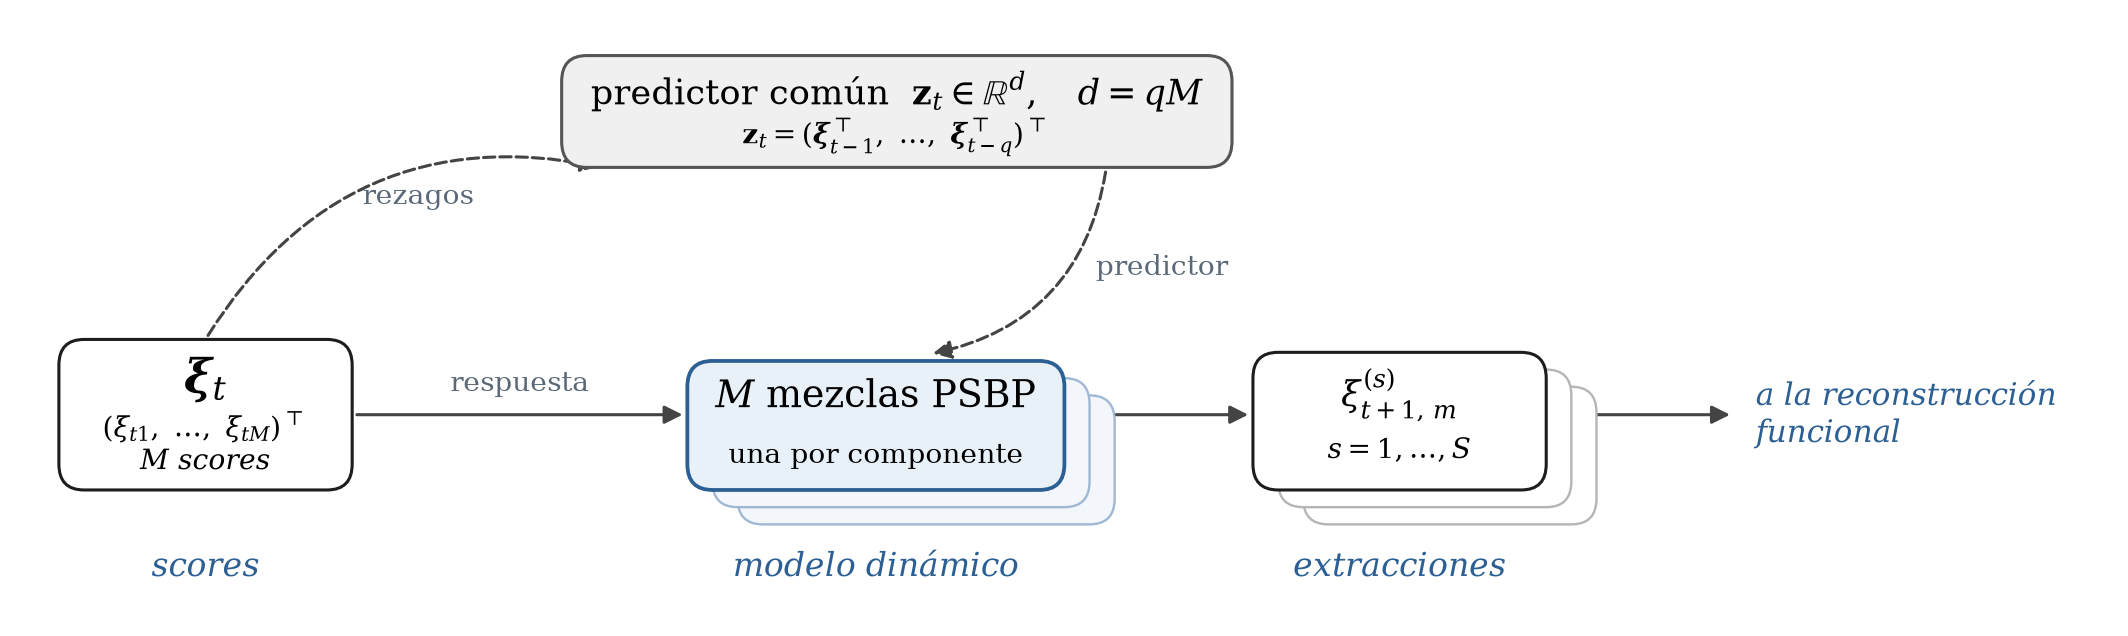
\includegraphics[width=\textwidth]{IMG/03_04/esquema_inferencia_psbpm_fd.png}
    \caption[Esquema de inferencia del PSBPM-FD]{Esquema de inferencia del
    PSBPM-FD. Cada mezcla toma como respuesta el score $\xi_{tm}$ de su
    componente y como predictor el vector común $\mathbf{z}_t$, de modo que el
    rezago de cualquier componente puede influir sobre la ley de cualquier otra.
    Su salida son $S$ extracciones de la predictiva a posteriori.}
    \label{fig:esquema_inferencia_psbpm_fd}
\end{figure}

Sobre estos datos se aplica sin modificación el muestreador de Gibbs descrito en la Sección~\ref{03_03_02_esquema_inferencia_bayesiana}, sustituyendo $y_i$ por $\xi_{tm}$ y $x_i$ por $\mathbf{z}_t$, sobre los $T_0 - q$ pares disponibles en un bloque de entrenamiento de longitud $T_0$. La factorización \eqref{eq:factorizacion} descompone la verosimilitud en el producto de las $M$ verosimilitudes individuales, de manera que los muestreadores son mutuamente independientes.\\

Cada uno entrega una colección de extracciones $\boldsymbol{\Omega}_m^{(s)}$, con $s = 1, \dots, S$, provenientes de la distribución a posteriori $p(\boldsymbol{\Omega}_m \mid \mathcal{D})$ tras descartar el período de calentamiento, donde $\boldsymbol{\Omega}_m$ agrupa los parámetros de pesos y átomos de la $m$-ésima mezcla y $\mathcal{D}$ denota el bloque de entrenamiento. Las extracciones de varias cadenas se agrupan por concatenación. Estas colecciones constituyen la única representación disponible del posterior y son, en consecuencia, el insumo del que se derivan todas las cantidades desconocidas del análisis, que quedan así definidas como funcionales de las extracciones y no como estimaciones puntuales.\\

La primera de dichas cantidades es la distribución predictiva del score, obtenida marginalizando la incertidumbre sobre los parámetros,
\begin{equation}\label{eq:predictiva_posteriori_score}
    f\bigl(\xi_{tm} \mid \mathbf{z}_t, \mathcal{D}\bigr)
    = \int f\bigl(\xi_{tm} \mid \mathbf{z}_t, \boldsymbol{\Omega}_m\bigr)
      p\bigl(\boldsymbol{\Omega}_m \mid \mathcal{D}\bigr) d\boldsymbol{\Omega}_m
    \;\approx\; \frac{1}{S} \sum_{s=1}^{S}
      f\bigl(\xi_{tm} \mid \mathbf{z}_t, \boldsymbol{\Omega}_m^{(s)}\bigr),
\end{equation}
donde el integrando es la mezcla \eqref{eq:psbpm_fd_componente} evaluada en cada extracción. La predictiva es una mezcla de mezclas y no la evaluación de \eqref{eq:psbpm_fd_componente} en una estimación puntual de $\boldsymbol{\Omega}_m$, distinción que resulta determinante para la incertidumbre reportada.\\

La aproximación~\eqref{eq:predictiva_posteriori_score} entrega la densidad predictiva en forma cerrada sobre una grilla, además su versión muestral se obtiene simulando en cada iteración el índice de componente desde la ley de pesos y a continuación la respuesta desde el átomo seleccionado, procedimiento cuya marginal es precisamente~\eqref{eq:predictiva_posteriori_score} y que basta ejecutar una vez por iteración retenida.


\section{Reconstrucción Funcional}
\label{03_05_00_reconstruccion_funcional}

El objeto de interés del estudio no es el score sino la curva, de modo que la predictiva de $\boldsymbol{\xi}_t$ dado $\mathbf{z}_t$, obtenida en $\mathbb{R}^{M}$, debe transportarse al espacio funcional. La descomposición que dio origen a los scores provee esa transformación, ya que la expansión \eqref{eq:expansion_kl_truncada} es un mapa lineal que asigna a cada vector de $\mathbb{R}^{M}$ una curva del subespacio generado por las autofunciones retenidas, y basta recorrerla en sentido inverso al empleado para construir la representación. Proyectando el vector de scores sobre dichas autofunciones, la curva queda escrita como
\begin{equation}\label{eq:reconstruccion_fpca}
    X_t^{(M)}(\tau_g) = \mu(\tau_g)
    + \sum_{m=1}^{M} \xi_{tm}v_m(\tau_g),
    \qquad g = 1, \dots, G,
\end{equation}
donde $\mu(\tau_g)$ y $v_m(\tau_g)$ denotan la función media y las autofunciones evaluadas en la grilla del dominio.\\

La expresión \eqref{eq:reconstruccion_fpca} es una identidad entre el vector de scores y la curva que representa, y adquiere carácter predictivo al evaluarla en el vector aleatorio cuya ley es la predictiva del modelo. Sustituyendo en ella $\boldsymbol{\xi}_t \mid \mathbf{z}_t, \mathcal{D}$ se induce la distribución predictiva de $X_t^{(M)}$ dado el estado rezagado, que es el objeto de interés del pronóstico. Como $\mu(\tau_g)$ y $\{v_m\}$ se tratan como conocidas, el mapa es determinista y afín, propiedad de la que se sigue que los momentos condicionales de la curva se obtengan en forma cerrada a partir de los momentos condicionales de los scores y que cada extracción predictiva de los scores, transportada por el mapa, sea una extracción exacta de la predictiva funcional condicional.\\


La predictiva funcional es por tanto una mezcla, y puede ser multimodal cuando los pesos $\pi_{hm}(\mathbf{z}_t)$ reparten la masa entre átomos de medias separadas; cuántos modos llegan a la curva no se lee de los pesos sino de las extracciones (Sección~\ref{03_06_00_comportamientos}).

\subsection{Esperanza predictiva}
\label{03_05_01_esperanza}

Aplicando el operador esperanza condicional a \eqref{eq:reconstruccion_fpca}, y observando que $\mu(\tau_g)$ y $v_m(\tau_g)$ son constantes que salen del operador, su linealidad entrega
\begin{equation}\label{eq:esperanza_curva}
    \mathbb{E}\bigl[X_t^{(M)}(\tau_g) \mid \mathbf{z}_t, \mathcal{D}\bigr]
    = \mu(\tau_g)
    + \sum_{m=1}^{M} \mathbb{E}\bigl[\xi_{tm} \mid \mathbf{z}_t, \mathcal{D}\bigr]v_m(\tau_g).
\end{equation}
La esperanza predictiva de la curva queda determinada por las $M$ esperanzas predictivas de los scores, sin aproximación adicional.\\

La esperanza de cada score se obtiene de \eqref{eq:predictiva_posteriori_score}. Para una extracción $\boldsymbol{\Omega}_m^{(s)}$, la media de la mezcla es la suma de las medias de sus átomos ponderada por los pesos,
\begin{equation}\label{eq:momento1_iteracion}
    \bar{\mu}_{tm}^{(s)} = \sum_{h=1}^{N} \pi_{hm}^{(s)}\mu_{hm}^{(s)},
    \qquad
    \pi_{hm}^{(s)} = \pi_{hm}\bigl(\mathbf{z}_t; \boldsymbol{\Omega}_m^{(s)}\bigr),
    \quad
    \mu_{hm}^{(s)} = \beta_{0,hm}^{*(s)} + \mathbf{z}_t^\top\boldsymbol{\beta}_{hm}^{*(s)},
\end{equation}
y la esperanza predictiva es el promedio de dichas medias sobre las $S$ extracciones,
\begin{equation}\label{eq:esperanza_score_estimada}
    \widehat{\mathbb{E}}\bigl[\xi_{tm} \mid \mathbf{z}_t, \mathcal{D}\bigr]
    = \frac{1}{S}\sum_{s=1}^{S} \bar{\mu}_{tm}^{(s)}.
\end{equation}
El orden de las operaciones no es intercambiable, ya que $\bar{\mu}_{tm}^{(s)}$ es un funcional de la mezcla completa e invariante a permutaciones de las etiquetas $h$, mientras que los parámetros individuales de cada átomo no lo son.\\


\subsection{Extracciones de la predictiva funcional}
\label{03_05_03_extracciones}

Para cada extracción $s$ de los parámetros y cada componente $m$ se obtiene una extracción del score en dos pasos, primero el índice del átomo, con los pesos evaluados en $\mathbf{z}_t$, y a continuación la respuesta desde el átomo seleccionado,
\begin{equation}\label{eq:extraccion_score}
    h_m^{(s)} \sim \text{Categórica}\Bigl(\pi_{1m}^{(s)}, \dots, \pi_{Nm}^{(s)}\Bigr),
    \qquad
    \xi_{tm}^{(s)} \sim \mathcal{N}\Bigl(\mu_{h_m^{(s)}m}^{(s)},
    \bigl(\nu_{h_m^{(s)}m}^{*(s)}\bigr)^{-1}\Bigr).
\end{equation}
Las $M$ extracciones de una misma iteración $s$ se apilan en un vector, lo que es legítimo bajo la factorización \eqref{eq:factorizacion}, y se transportan a la curva mediante \eqref{eq:reconstruccion_fpca},
\begin{equation}\label{eq:extraccion_curva}
    \widehat{X}_{t}^{(s)}(\tau_g) = \mu(\tau_g)
    + \sum_{m=1}^{M} \xi_{tm}^{(s)}v_m(\tau_g),
    \qquad s = 1, \dots, S.
\end{equation}
Al ser \eqref{eq:reconstruccion_fpca} un mapa determinista, las curvas así construidas son extracciones exactas de la predictiva funcional y la muestra $\{\widehat{X}_t^{(s)}\}_{s=1}^{S}$ es la representación de esa ley. Las curvas se extraen sobre una submuestra equiespaciada de las iteraciones del posterior, una por iteración retenida; en esta sección y en la siguiente, $S$ denota el tamaño de esa submuestra.\\

Al muestrear de este modo, cada extracción elige primero un átomo y luego extrae de él, de manera que la muestra mezcla las extracciones de todos los átomos con peso en $\mathbf{z}_t$ sin registrar de cuál proviene cada una. Si dos o más átomos reciben peso apreciable y sus medias condicionales están separadas, la muestra resulta multimodal y por tanto las extracciones se agrupan en torno a la media de cada átomo. Esa multimodalidad es una propiedad de la mezcla en $\mathbf{z}_t$, no del muestreo, y existiría aunque los parámetros fuesen conocidos. 

\subsection{Predictores puntuales de la curva}
\label{03_05_04_predictores_puntuales}

La esperanza de la Sección~\ref{03_05_01_esperanza} es el predictor puntual óptimo bajo pérdida cuadrática cualquiera sea la forma de la predictiva, y describe bien lo que el modelo espera cuando esta es unimodal y simétrica, por ejemplo cuando los pesos $\pi_{hm}(\mathbf{z}_t)$ concentran la masa en un solo átomo. Cuando la predictiva resulta multimodal o asimétrica, lo que suele indicar que el estado rezagado $\mathbf{z}_t$ no separa por completo los regímenes de la mezcla, la esperanza pasa a ser un promedio de comportamientos posibles que no coincide con ninguno de ellos. Por eso se presentan dos predictores menos sensibles a esos efectos, calculados sobre las extracciones de la Sección~\ref{03_05_03_extracciones}.
 

\subsubsection{Mediana puntual}
\label{03_05_04_01_mediana_puntual}

Denotando por $\widehat{F}_{t,g}$ la función de distribución empírica de la muestra en el punto $\tau_g$,
\begin{equation}\label{eq:fdist_empirica}
    \widehat{F}_{t,g}(y) = \frac{1}{S}\sum_{s=1}^{S}
    \mathbf{1}\bigl\{\widehat{X}_{t}^{(s)}(\tau_g) \leq y\bigr\},
\end{equation}
la mediana puntual es la curva $\widehat{X}_t^{\mathrm{med}}(\tau_g) = \widehat{F}_{t,g}^{-1}(1/2)$. Como el error absoluto funcional es una integral de errores absolutos en cada punto, la mediana puntual lo minimiza punto a punto y es el predictor consistente con esa métrica. Su limitación es que no es necesariamente una curva que el modelo genere, ya que en cada punto del dominio toma la mediana de las extracciones, y si en una parte del dominio domina un grupo de extracciones y en otra parte domina otro, el resultado junta tramos de curvas distintas. 

\subsubsection{Átomo más probable}
\label{03_05_04_02_atomo_modal}
 En cada iteración $s$ y componente $m$ se toma el átomo de mayor peso en $\mathbf{z}_t$ y su media condicional,
\begin{equation}\label{eq:atomo_modal}
    h_m^{\star(s)} = \operatorname*{argmax}_{h} \pi_{hm}^{(s)},
    \qquad
    \xi_{tm}^{\mathrm{mod}} = \operatorname{mediana}_{s}\mu_{h_m^{\star(s)} m}^{(s)},
\end{equation}
y la curva modal se obtiene transportando el vector $\boldsymbol{\xi}_t^{\mathrm{mod}}$ por \eqref{eq:reconstruccion_fpca}. Se trata, en cada iteración, del predictor óptimo bajo pérdida cero-uno sobre la asignación de régimen de cada componente, y su cálculo es exacto, ya que la ley conjunta de los $M$ scores es una mezcla sobre configuraciones $(h_1, \dots, h_M)$ con pesos $\prod_m \pi_{h_m m}^{(s)}$, de modo que, al maximizarse un producto de factores independientes factor a factor, la configuración más probable es la que toma el átomo más probable de cada componente. La agregación sobre $s$ se realiza mediante la mediana y no mediante el promedio, con el fin de evitar que las iteraciones en que los pesos $\pi_{hm}^{(s)}$ se reparten casi por igual entre dos átomos desplacen el predictor hacia la región entre ambos. Este predictor responde a cómo sería la curva si se realizara el régimen más probable y acompaña de modo natural a la probabilidad de ese régimen.\\

Los tres predictores coinciden aproximadamente cuando la predictiva es unimodal y simétrica, y se separan en la medida en que no lo es. 

\subsection{Intervalos de credibilidad predictivos}
\label{03_05_05_intervalos_predictivos}

Los intervalos se construyen a partir de los cuantiles empíricos de las extracciones y no como intervalos simétricos en torno a la esperanza, que impondrían por construcción la simetría y unimodalidad que el modelo existe para no suponer.\\


\subsubsection{Intervalo puntual equi-colas}
\label{03_05_05_01_equicolas}
Con la distribución empírica \eqref{eq:fdist_empirica}, el intervalo de credibilidad de nivel $1-\zeta$ en cada punto del dominio es
\begin{equation}\label{eq:intervalo_puntual}
    \Bigl[\widehat{F}_{t,g}^{-1}(\zeta/2),\;
    \widehat{F}_{t,g}^{-1}(1-\zeta/2)\Bigr],
    \qquad g = 1, \dots, G.
\end{equation}
El intervalo así construido es puntual y no simultáneo.

\subsubsection{Banda simultánea}
\label{03_05_05_02_banda_simultanea}
Cuando el objeto de interés es la curva completa, la banda debe calibrarse para que contenga la curva entera con probabilidad $1-\zeta$. Con la mediana puntual como centro $\widehat{X}_t^{\mathrm{med}}(\tau_g)$ y como escala $\widehat{\sigma}_t(\tau_g)$ el rango intercuartílico de la muestra dividido por $1.349$, ambos robustos frente a las colas no acotadas de los átomos cuando $a_\nu \le 1$, se define la desviación máxima normalizada de cada extracción,
\begin{equation}\label{eq:supnorma}
    D^{(s)} = \max_{g}\;\frac{\bigl|\widehat{X}_t^{(s)}(\tau_g) - \widehat{X}_t^{\mathrm{med}}(\tau_g)\bigr|}{\widehat{\sigma}_t(\tau_g)},
\end{equation}
y la banda $\widehat{X}_t^{\mathrm{med}}(\tau_g) \pm q_{1-\zeta}(D)\widehat{\sigma}_t(\tau_g)$, con $q_{1-\zeta}(D)$ el cuantil empírico de $\{D^{(s)}\}$, contiene por construcción a una fracción $1-\zeta$ de las extracciones en toda su extensión. Es la banda de tipo supremo de \citet{03_05_degras2011bands} evaluada sobre la predictiva. Esta banda tiene una limitación cuando la predictiva es multimodal, porque al ser una región conexa cubre también el valle entre las cumbres.

\subsubsection{Región de máxima densidad}
\label{03_05_05_03_hdr}

La región de máxima densidad de nivel $1-\zeta$ \citep{03_05_hyndman1996hdr} es el conjunto de menor medida que acumula probabilidad $1-\zeta$,
\begin{equation}\label{eq:hdr}
    \mathcal{R}_{1-\zeta} = \bigl\{y : f(y) \geq f_{\zeta}\bigr\},
    \qquad
    \Pr\bigl(Y \in \mathcal{R}_{1-\zeta}\bigr) = 1-\zeta,
\end{equation}
con $f$ la densidad predictiva. Con una predictiva unimodal y simétrica coincide con el intervalo equi-colas, mientras que con dos modos separados por un valle cuya densidad cae bajo $f_\zeta$ es la unión de dos intervalos, uno por modo, cuya longitud total es menor que la del intervalo central al mismo nivel porque excluye el valle. Es la contraparte, para intervalos, de la observación de la Sección~\ref{03_05_04_predictores_puntuales} sobre la esperanza.\\

En el caso funcional la región se construye punto a punto sobre el dominio, del mismo modo que el intervalo \eqref{eq:intervalo_puntual}. En cada $\tau_g$ se estima por núcleo la densidad de la muestra $\{\widehat{X}_t^{(s)}(\tau_g)\}_{s=1}^{S}$ y se toma el conjunto \eqref{eq:hdr}, que donde la predictiva es unimodal y simétrica coincide con el intervalo equi-colas y donde es multimodal puede descomponerse en varios tramos.\\

El puntaje de Winkler se extiende a una región de este tipo sumando las longitudes de sus tramos y penalizando por la distancia de la observación al tramo más cercano, y del mismo modo el MPIW suma las longitudes de los tramos y el PICP cuenta si la observación cae en alguno de ellos, de manera que las tres construcciones se comparan con las métricas de la Sección~\ref{02_02_03_criterios_evaluacion}. Cabe tener presente que el funcional que el puntaje de Winkler elicita es el intervalo central, de modo que la región de máxima densidad no tiene por qué mejorarlo aun cuando sea más angosta.

\section{Comportamientos predictivos}
\label{03_06_00_comportamientos}
En cada iteración, la predictiva conjunta de los scores es una mezcla sobre configuraciones de átomos $(h_1, \dots, h_M)$ con pesos $\prod_m \pi_{h_m m}^{(s)}$, y la forma que toma depende de cuánto informa el estado rezagado $\mathbf{z}_t$ sobre el régimen. Si lo determina, los pesos concentran la masa en átomos de un mismo régimen y la predictiva tiene un solo modo, si no lo determina, la masa se reparte entre átomos de regímenes distintos, y por tanto la predictiva tiene un modo por cada uno. A cada uno de esos modos se le llama comportamiento predictivo.\\

Los comportamientos se identifican origen por origen, como parte de la predicción de cada curva, y de cada uno se obtienen su probabilidad, su curva típica y su dispersión. Así pueden contrastarse con los regímenes del proceso cuando se conocen, o con una variable que los represente cuando no. Los modelos de referencia, cuya predictiva es unimodal, no admiten esta descomposición.\\

Los comportamientos no pueden leerse de los parámetros, ya que los átomos de componentes distintas no se corresponden entre sí, un mismo régimen puede repartirse en varios átomos equivalentes y el peso de una configuración completa, al ser un producto de $M$ pesos, no se interpreta como la probabilidad de un comportamiento. Lo único que vincula a las $M$ mezclas es $\mathbf{z}_t$, de modo que los comportamientos se identifican sobre las extracciones, que son extracciones de la predictiva conjunta en ese $\mathbf{z}_t$. 
 
\subsection{Agrupamiento de las extracciones}
\label{03_06_01_agrupamiento}

Como las autofunciones son ortonormales en $L^2$, la distancia euclídea entre dos vectores de scores coincide con la distancia $L^2$ entre las curvas que representan, de modo que basta agrupar las extracciones en $\mathbb{R}^{M}$ con los scores. Para cada origen $t$ se agrupan las $S$ extracciones $\{\boldsymbol{\xi}_t^{(s)}\}$ mediante $k$-medias, esto es, se busca la partición en $K$ grupos $\mathcal{G}_1, \dots, \mathcal{G}_K$ que minimiza la suma de cuadrados dentro de los grupos,
\begin{equation}\label{eq:kmedias}
    \min_{\mathcal{G}_1, \dots, \mathcal{G}_K}\ \sum_{k=1}^{K}\ \sum_{s \in \mathcal{G}_k} \bigl\lVert \boldsymbol{\xi}_t^{(s)} - \bar{\boldsymbol{\xi}}_{t,k} \bigr\rVert^{2},
    \qquad
    \bar{\boldsymbol{\xi}}_{t,k} = \frac{1}{\lvert \mathcal{G}_k \rvert}\sum_{s \in \mathcal{G}_k} \boldsymbol{\xi}_t^{(s)},
\end{equation}
resuelta alternando la asignación de cada extracción al centroide más cercano con el recálculo de los centroides como medias de sus grupos, desde varios inicios aleatorios.\\

La fracción de varianza explicada por la partición, $R^2_K = 1 - \mathrm{SCD}_K / \mathrm{SCD}_1$ con $\mathrm{SCD}_K$ el mínimo de \eqref{eq:kmedias}, crece con $K$ aunque no exista estructura, de manera que el número de comportamientos no puede fijarse por un umbral sobre ella y se decide con las tres reglas de la Sección~\ref{03_06_02_numero}. Cuando la distribución a priori de las precisiones admite átomos de varianza no acotada, las extracciones se recortan a los cuantiles extremos de cada score antes del agrupamiento.

\subsection{Número de comportamientos}
\label{03_06_02_numero}

La primera regla decide si existe más de un comportamiento. Con $K = 2$, las extracciones se proyectan sobre el eje que une los dos centroides, $\mathbf{d}_t = (\bar{\boldsymbol{\xi}}_{t,2} - \bar{\boldsymbol{\xi}}_{t,1}) / \lVert \bar{\boldsymbol{\xi}}_{t,2} - \bar{\boldsymbol{\xi}}_{t,1} \rVert$, y sobre la proyección se estima por núcleo la densidad $\widehat{f}$. Se declara que hay dos modos si la densidad entre los centroides desciende por debajo de la mitad de la menor de las densidades evaluadas en ellos,
\begin{equation}\label{eq:valle}
    \frac{\min_{x_1 \le x \le x_2} \widehat{f}(x)}{\min\bigl\{\widehat{f}(x_1), \widehat{f}(x_2)\bigr\}} < \tfrac{1}{2},
    \qquad x_1 = \bar{\boldsymbol{\xi}}_{t,1}^\top \mathbf{d}_t,\ \ x_2 = \bar{\boldsymbol{\xi}}_{t,2}^\top \mathbf{d}_t,
\end{equation}
y en caso contrario se declara un único comportamiento. Esta regla es una versión operativa del contraste de unimodalidad de \citet{03_05_hartigan1985dip}, y es la que distingue una predictiva con dos modos de una unimodal alargada o asimétrica, que $k$-medias también parte en dos pero sin que la densidad presente un valle.\\

La segunda regla acota el número de comportamientos. A partir de $K = 2$ se acepta la partición en $K + 1$ grupos solo si el grupo adicional explica al menos tanto como explica en promedio cada uno de los existentes,
\begin{equation}\label{eq:crecimiento}
    R^2_{K+1} \;\geq\; R^2_K + \frac{R^2_K}{K},
\end{equation}
condición equivalente a que la varianza explicada por comportamiento no disminuya, y el barrido se detiene en el primer $K$ que la incumple.\\

La tercera regla exige que cada comportamiento reúna una masa de al menos $\zeta$, el nivel de la banda de credibilidad, de manera que un comportamiento sea un grupo de extracciones que la banda al nivel $1-\zeta$ tendría que cubrir; un grupo de masa menor es una cola y no un comportamiento, y la partición que lo produce se descarta. Las tres reglas dependen de dos constantes, el cociente de valle y $\zeta$.

\subsection{Probabilidad, curva típica, pronóstico por comportamiento y su cota}
\label{03_06_03_descripcion}

El resultado por origen es un conjunto de $K_t$ comportamientos. Cada uno tiene probabilidad $p_{t,k} = \lvert \mathcal{G}_k \rvert / S$, igual a la fracción de extracciones del grupo, curva típica $\widehat{X}_{t,k}$ igual al centroide $\bar{\boldsymbol{\xi}}_{t,k}$ transportado por \eqref{eq:reconstruccion_fpca}, que por linealidad del mapa es la esperanza predictiva condicional a ese comportamiento, e intervalo condicional dado por los cuantiles equi-colas \eqref{eq:intervalo_puntual} calculados solo sobre las extracciones del grupo. La mezcla de las curvas típicas ponderada por sus probabilidades es la media de las extracciones recortadas, que aproxima a la esperanza predictiva de la Sección~\ref{03_05_01_esperanza},
\begin{equation}\label{eq:esperanza_por_comportamientos}
    \widehat{\mathbb{E}}\bigl[X_t^{(M)}(\tau_g) \mid \mathbf{z}_t, \mathcal{D}\bigr]
    \approx \sum_{k=1}^{K_t} p_{t,k}\widehat{X}_{t,k}(\tau_g),
\end{equation}
relación que muestra por qué, con más de un comportamiento, la esperanza se sitúa entre ellos. El contraste entre dos comportamientos es la diferencia de sus curvas típicas, $\Delta_{t,kk'}(\tau_g) = \widehat{X}_{t,k}(\tau_g) - \widehat{X}_{t,k'}(\tau_g)$, que localiza en qué parte del dominio difieren y en cuánto.\\

Los comportamientos permiten un predictor puntual distinto de los de la Sección~\ref{03_05_04_predictores_puntuales}. Aquellos resumen la predictiva completa, y por \eqref{eq:esperanza_por_comportamientos} la esperanza queda entre los comportamientos cuando hay más de uno, mientras que la mediana puntual elige entre modos de forma indirecta y el átomo más probable lo hace componente a componente en el espacio de los scores. El pronóstico por comportamiento elige de forma explícita un modo de la predictiva conjunta, ya que se toma el comportamiento de mayor probabilidad y se predice con su curva típica,
\begin{equation}\label{eq:pronostico_comportamiento}
    \widehat{X}_t^{\mathrm{mp}}(\tau_g) = \widehat{X}_{t,k_t^{*}}(\tau_g),
    \qquad
    k_t^{*} = \arg\max_{k = 1, \ldots, K_t} p_{t,k}.
\end{equation}
Con $K_t = 1$ se toma la esperanza predictiva de la Sección~\ref{03_05_01_esperanza}, de modo que el predictor solo se aparta de ella en los orígenes en que la predictiva tiene más de un modo, y ahí lo hace comprometiéndose con uno de ellos en lugar de promediarlos. Del mismo modo, es natural extender a cada comportamiento los otros dos predictores de la Sección~\ref{03_05_04_predictores_puntuales}, la mediana puntual y el átomo más probable, calculados solo sobre las extracciones del comportamiento elegido (y, con $K_t = 1$, sobre la predictiva completa); la mediana puntual es la variante del mismo predictor para una condicional asimétrica.\\

El pronóstico \eqref{eq:pronostico_comportamiento} es una regla de elección entre los $K_t$ comportamientos, y conviene separar lo que pierde por elegir de lo que la predictiva no contiene. Para eso se define su cota, el mejor comportamiento, como la curva típica del comportamiento más cercano en $L^2$ a la curva observada,
\begin{equation}\label{eq:mejor_comportamiento}
    \widehat{X}_t^{\mathrm{cota}}(\tau_g) = \widehat{X}_{t,k_t^{\circ}}(\tau_g),
    \qquad
    k_t^{\circ} = \arg\min_{k = 1, \ldots, K_t} \bigl\lVert X_t - \widehat{X}_{t,k} \bigr\rVert,
\end{equation}
que con $K_t = 1$ coincide con el pronóstico. No es un predictor, porque elige con la observación, sino una cota, el menor error que puede alcanzar cualquier regla que pronostique con uno de los comportamientos. La distancia entre el pronóstico y su cota mide lo que cuesta elegir con la probabilidad en vez de con la curva observada, y la distancia entre la cota y la esperanza, cuánto hay que ganar si se eligiera bien. Además permite ver si la curva que ocurre está entre las opciones que la predictiva entrega, de modo que, cuando la cota queda por debajo de las referencias y el pronóstico no, la desventaja está en resumir la predictiva en una curva y no en la información que contiene.


\section{Diseño del Estudio de Simulación}
\label{03_07_00_diseno_estudio_simulacion}

El estudio aborda tres preguntas de evaluación: ¿en cuáles de los tres escenarios la predicción puntual del PSBPM-FD supera a la de los modelos de referencia?, ¿en cuáles sus intervalos de credibilidad ofrecen un mejor desempeño? y, en el escenario con cambio de régimen, ¿en qué medida los comportamientos de su distribución predictiva reproducen los regímenes del proceso y permiten generar pronósticos a partir de ellos? La evaluación se realiza mediante las métricas definidas en la Sección~\ref{02_02_03_criterios_evaluacion}.\\

En los tres escenarios el procedimiento es el mismo, las curvas se generan con el esquema común del Anexo~\ref{ane_00_01_esquema_comun} y se parten en orden cronológico en un bloque de entrenamiento ($70\%$) y uno de prueba. Las predicciones a un paso sobre el segundo usan los rezagos observados, sin reestimar.\\

Las métricas de la Sección~\ref{02_02_03_criterios_evaluacion} se calculan sobre la ventana móvil de ancho $w_{\mathrm{ref}} = 30$, contra la curva ajustada por la representación (Sección~\ref{03_05_00_reconstruccion_funcional}), para cada $M$ del barrido. El PSBPM-FD se ajusta con los hiperparámetros de \citet{03_02_chung2009nonparametric} llevados a la escala de cada score.\\

Las referencias son el FAR, con orden fijo igual al número de rezagos del escenario e intervalo gaussiano, y el Random Forest con la misma especificación que el PSBPM-FD. Se reportan el MAE y el RMSE de los tres predictores puntuales, del pronóstico por comportamiento (Sección~\ref{03_06_03_descripcion}) y de su cota \eqref{eq:mejor_comportamiento}, estos dos solo en C-2, cada uno contra el FAR y el Random Forest; y el Winkler, el MPIW y el PICP de las tres construcciones de intervalo contra el FAR.\\

Los comportamientos predictivos y el pronóstico que se construye con ellos se evalúan solo en C-2, el escenario cuya ley condicional reparte su masa entre regímenes separados. En C-1 la media condicional es única y en C-3 la multimodalidad queda en la ley conjunta de los scores y no llega a la marginal de cada score ni a la de la curva, de modo que en ambos se espera que la predictiva tenga un solo comportamiento y el pronóstico por comportamiento coincida con la esperanza, lo que la Sección~\ref{03_08_03_comportamientos} confirma. En C-2 los comportamientos se resumen por la distribución de $K_t$ en el bloque de prueba y, origen a origen, en una ventana de detalle de $N_{\mathrm{det}} = 10$ orígenes consecutivos, la de más cambios de régimen verdadero, elegida con lo que el generador registra y nunca con lo predicho. La configuración completa está en el Anexo~\ref{ane_00_03_configuracion} y las métricas restantes y los otros anchos de ventana, en el Anexo~\ref{aneB_00_00_resultados_simulacion}.

\subsection{Escenarios}
\label{03_07_02_escenarios}

Cada escenario introduce un rasgo de la ley condicional del score que un modelo de media lineal no representa; los algoritmos y sus valores están en el Anexo~\ref{ane_00_00_anexo}. En los tres la dinámica vive en los $J_a = 4$ primeros scores y los restantes son autorregresivos de primer orden, de modo que $M = 4$ es la primera dimensión que observa toda la dinámica.\\

El régimen o mecanismo que sortea el generador se registra pero no se entrega a ningún método. El Cuadro~\ref{tab:dis_escenarios} resume la configuración de cada escenario, con $q$ el número de rezagos. Con rezagos propios, la mezcla de la componente $m$ recibe solo $(\xi_{t-1,m}, \dots, \xi_{t-q,m})^\top$, la restricción de $\mathbf{z}_t$ a sus propios rezagos, de modo que $d = q$; con los rezagos de todas las componentes, $d = qM$.

\begin{table}[H]
\centering\small
\setlength{\tabcolsep}{4pt}
\caption{Escenarios del estudio y configuración de los métodos en cada uno.}
\label{tab:dis_escenarios}
\begin{tabular}{p{0.07\textwidth} p{0.30\textwidth} p{0.14\textwidth} p{0.05\textwidth} p{0.20\textwidth} p{0.10\textwidth}}
\hline
 & Rasgo & Algoritmo & $q$ & Covariables & $M$ \\
\hline
C-1 & Heterocedasticidad condicional        & Anexo~\ref{ane_00_02_01_alg_c1} & $4$ & Rezagos propios                       & $1,\ldots,10$ \\
C-2 & Cambio de régimen por umbral          & Anexo~\ref{ane_00_02_02_alg_c2} & $4$ & Rezagos propios                       & $1,\ldots,10$ \\
C-3 & Multimodalidad en la ley conjunta de los scores & Anexo~\ref{ane_00_02_03_alg_c3} & $2$ & Rezagos de todas las componentes & $3,\ldots,6$ \\
\hline
\end{tabular}
\end{table}

\begin{itemize}
    \item \textbf{C-1.} Los scores activos son autorregresivos con innovaciones GARCH$(1,1)$. La media condicional es lineal y la no linealidad está únicamente en la varianza, con una memoria de unas siete curvas. Como la señal de volatilidad depende de los dos rezagos propios más próximos, el modelo puede aprenderla, por lo que la ventaja esperable del PSBPM-FD está en los intervalos de credibilidad y no en la predicción puntual.

    \item \textbf{C-2.} Cada score activo alterna, mediante una transición probit dependiente de su propio rezago, entre un régimen persistente de escala pequeña y otro más volátil y con reversión. La media condicional es no lineal y la varianza depende del estado. La calibración favorece deliberadamente la separación entre regímenes, por lo que las conclusiones se limitan a esta configuración.

       \item \textbf{C-3.} Un softmax sobre los dos rezagos de los dos primeros scores selecciona entre tres mecanismos lineales, uno central y dos con niveles distintos, cuyas localizaciones difieren en más que la escala de la innovación. Esto genera una ley condicional multimodal en el espacio conjunto de los scores, aunque la media condicional sea casi lineal y la marginal de cada score quede casi unimodal. Como el mecanismo depende de los rezagos de $\xi_1$ y $\xi_2$, las covariables incluyen los rezagos de todas las componentes y el muestreador se ejecuta para cada valor de $M$.
\end{itemize}


\section{Resultados}
\label{03_08_00_resultados}

Cada apartado de esta sección responde a una de las preguntas del diseño con la misma lectura en tres niveles, el promedio sobre las ventanas de prueba para cada $M$ del barrido, la fracción de ventanas que gana cada modelo en $M_{\mathrm{ref}}$, y la trayectoria de la métrica a lo largo del bloque de prueba, de modo que una diferencia en el promedio pueda atribuirse a una ventaja sostenida o a unos pocos tramos.\\

Todas las cifras son contra la curva ajustada por la representación, con la ventana de ancho $w_{\mathrm{ref}} = 30$ y, salvo indicación, con $M_{\mathrm{ref}} = 10$ en C-1 y C-2 y $M_{\mathrm{ref}} = 6$ en C-3. La Sección~\ref{03_08_01_error_puntual} compara los tres predictores puntuales del PSBPM-FD con el FAR y el Random Forest, la Sección~\ref{03_08_02_intervalos} hace lo propio con las tres construcciones de intervalo frente a la banda gaussiana del FAR, y las Secciones~\ref{03_08_03_comportamientos} y~\ref{03_08_04_pronostico}, restringidas a C-2, examinan cuántos comportamientos declara la predictiva, cómo se comparan con los de la ley verdadera y qué se gana y se pierde al pronosticar con el más probable.


\subsection{Error puntual}
\label{03_08_01_error_puntual}

Los Cuadros~\ref{tab:res_bloqueA} y~\ref{tab:res_bloqueA_rmse} resumen el MAE y el RMSE promedio sobre las ventanas de prueba, contra la curva ajustada, de los tres predictores puntuales del PSBPM-FD y de las dos referencias, para cada $M$ del barrido. Las Figuras~\ref{fig:res_bloqueA_vs_M_C1} a~\ref{fig:res_bloqueA_vs_M_C3} muestran las mismas cifras contra $M$ y el Cuadro~\ref{tab:res_bloqueA_ventanas}, en $M_{\mathrm{ref}}$, cómo se reparten las ventanas entre los modelos.

\begin{table}[H]
\centering\small
\setlength{\tabcolsep}{3.5pt}
\caption{MAE en el bloque de prueba por escenario y $M$. En negrita el menor en $M_{\mathrm{ref}}$.}
\label{tab:res_bloqueA}
\begin{tabular}{c cccc cccc cccc}
\hline
 & \multicolumn{4}{c}{C-1} & \multicolumn{4}{c}{C-2} & \multicolumn{4}{c}{C-3} \\
$M$ & Esp. & Med. & Modal & RF & Esp. & Med. & Modal & RF & Esp. & Med. & Modal & RF \\
\hline
$1$  & 0.754 & 0.755 & 0.755 & 0.764 & 0.714 & 0.720 & 0.725 & 0.710 & --- & --- & --- & --- \\
$2$  & 0.739 & 0.739 & 0.739 & 0.753 & 0.673 & 0.675 & 0.691 & 0.658 & --- & --- & --- & --- \\
$3$  & 0.724 & 0.724 & 0.726 & 0.740 & 0.635 & 0.633 & 0.652 & 0.617 & 0.694 & 0.695 & 0.703 & 0.699 \\
$4$  & 0.716 & 0.717 & 0.722 & 0.734 & 0.612 & 0.605 & 0.635 & 0.591 & 0.689 & 0.691 & 0.700 & 0.699 \\
$5$  & 0.714 & 0.714 & 0.719 & 0.733 & 0.610 & 0.603 & 0.633 & 0.591 & 0.684 & 0.685 & 0.693 & 0.693 \\
$6$  & 0.713 & 0.713 & 0.718 & 0.732 & 0.609 & 0.602 & 0.632 & 0.592 & \textbf{0.689} & 0.689 & 0.698 & 0.700 \\
$7$  & 0.712 & 0.713 & 0.718 & 0.733 & 0.609 & 0.601 & 0.631 & 0.592 & --- & --- & --- & --- \\
$8$  & 0.712 & 0.712 & 0.717 & 0.733 & 0.609 & 0.601 & 0.631 & 0.592 & --- & --- & --- & --- \\
$9$  & 0.711 & 0.712 & 0.717 & 0.734 & 0.609 & 0.601 & 0.631 & 0.591 & --- & --- & --- & --- \\
$10$ & \textbf{0.711} & 0.712 & 0.717 & 0.734 & 0.609 & 0.601 & 0.631 & \textbf{0.591} & --- & --- & --- & --- \\
\hline
FAR & \multicolumn{4}{c}{0.723} & \multicolumn{4}{c}{0.770} & \multicolumn{4}{c}{0.700} \\
\hline
\end{tabular}
\end{table}

% Fuente: 98_resumen_bloqueA_min_max_prom.csv del _05 (test, rmse_f).
\begin{table}[H]
\centering\small
\setlength{\tabcolsep}{3.5pt}
\caption{RMSE en el bloque de prueba por escenario y $M$. En negrita el menor en $M_{\mathrm{ref}}$.}
\label{tab:res_bloqueA_rmse}
\begin{tabular}{c cccc cccc cccc}
\hline
 & \multicolumn{4}{c}{C-1} & \multicolumn{4}{c}{C-2} & \multicolumn{4}{c}{C-3} \\
$M$ & Esp. & Med. & Modal & RF & Esp. & Med. & Modal & RF & Esp. & Med. & Modal & RF \\
\hline
$1$  & 0.951 & 0.953 & 0.953 & 0.967 & 0.906 & 0.920 & 0.927 & 0.906 & --- & --- & --- & --- \\
$2$  & 0.923 & 0.924 & 0.925 & 0.943 & 0.854 & 0.865 & 0.889 & 0.843 & --- & --- & --- & --- \\
$3$  & 0.903 & 0.904 & 0.908 & 0.927 & 0.808 & 0.816 & 0.849 & 0.793 & 0.870 & 0.872 & 0.880 & 0.878 \\
$4$  & 0.895 & 0.897 & 0.905 & 0.922 & 0.783 & 0.787 & 0.839 & 0.767 & 0.866 & 0.868 & 0.882 & 0.877 \\
$5$  & 0.893 & 0.894 & 0.903 & 0.921 & 0.781 & 0.783 & 0.837 & 0.766 & 0.860 & 0.861 & 0.872 & 0.870 \\
$6$  & 0.891 & 0.892 & 0.902 & 0.920 & 0.779 & 0.781 & 0.835 & 0.766 & \textbf{0.866} & 0.866 & 0.879 & 0.877 \\
$7$  & 0.891 & 0.892 & 0.901 & 0.920 & 0.778 & 0.780 & 0.834 & 0.766 & --- & --- & --- & --- \\
$8$  & 0.890 & 0.891 & 0.901 & 0.920 & 0.777 & 0.779 & 0.834 & 0.766 & --- & --- & --- & --- \\
$9$  & 0.890 & 0.891 & 0.901 & 0.920 & 0.777 & 0.779 & 0.833 & 0.766 & --- & --- & --- & --- \\
$10$ & \textbf{0.890} & 0.891 & 0.901 & 0.920 & 0.777 & 0.779 & 0.833 & \textbf{0.766} & --- & --- & --- & --- \\
\hline
FAR & \multicolumn{4}{c}{0.906} & \multicolumn{4}{c}{0.980} & \multicolumn{4}{c}{0.880} \\
\hline
\end{tabular}
\end{table}

% Figura Bloque A contra M: MAE y RMSE de los tres predictores, FAR y RF. Fuente: 98_* del _05.
\begin{figure}[H]
\centering
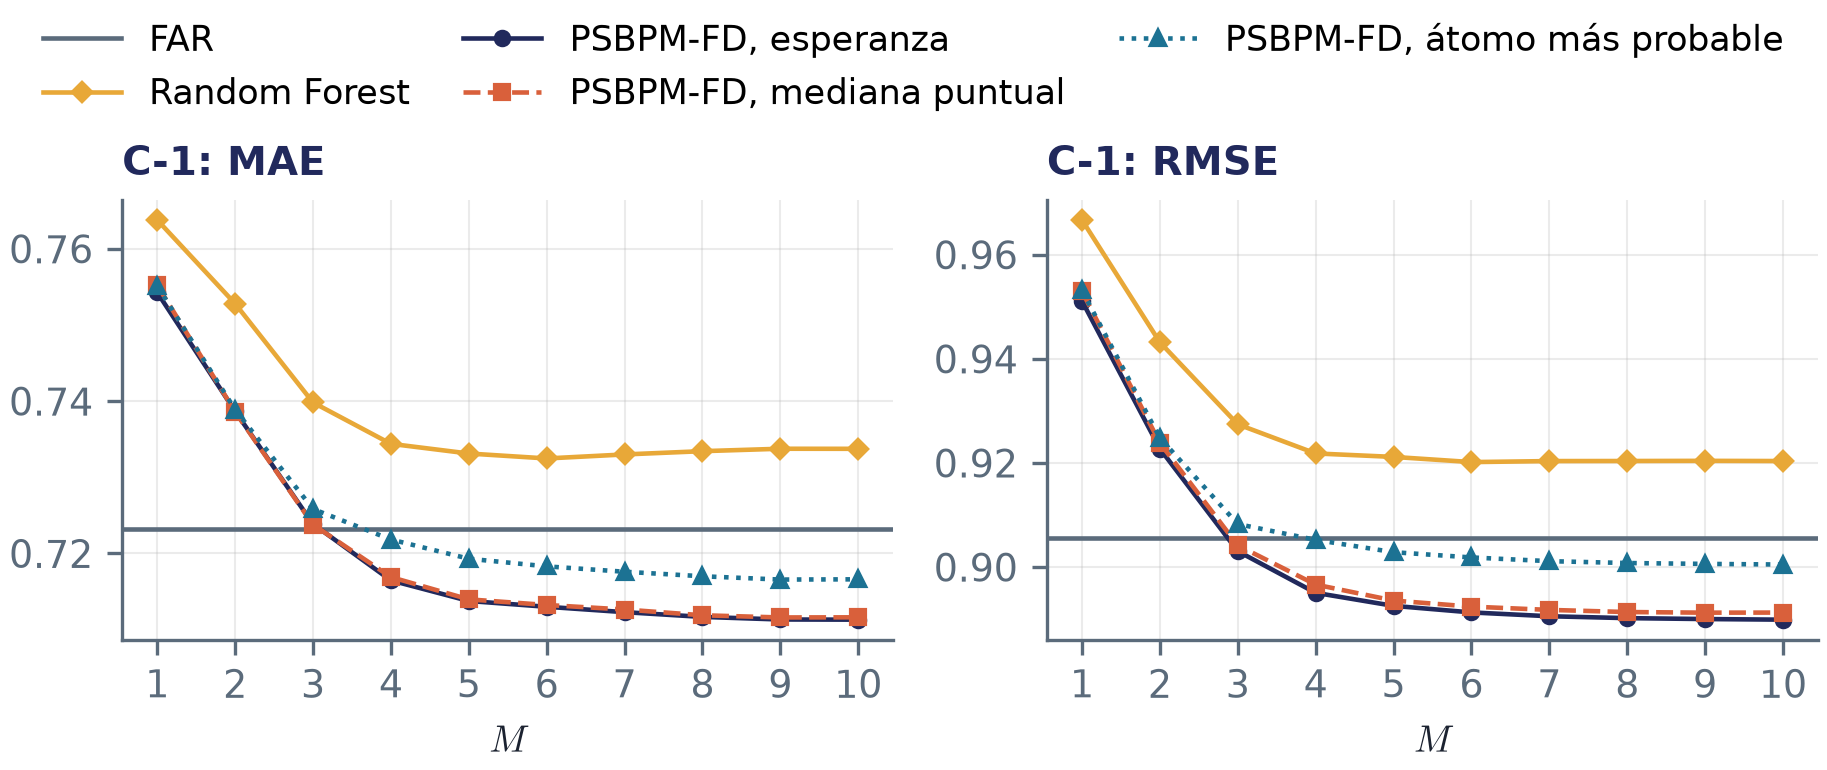
\includegraphics[width=\textwidth]{IMG/03_08/03_08_bloqueA_vs_M_C1.png}
\caption{C-1. MAE y RMSE en el bloque de prueba contra $M$.}
\label{fig:res_bloqueA_vs_M_C1}
\end{figure}

\begin{figure}[H]
\centering
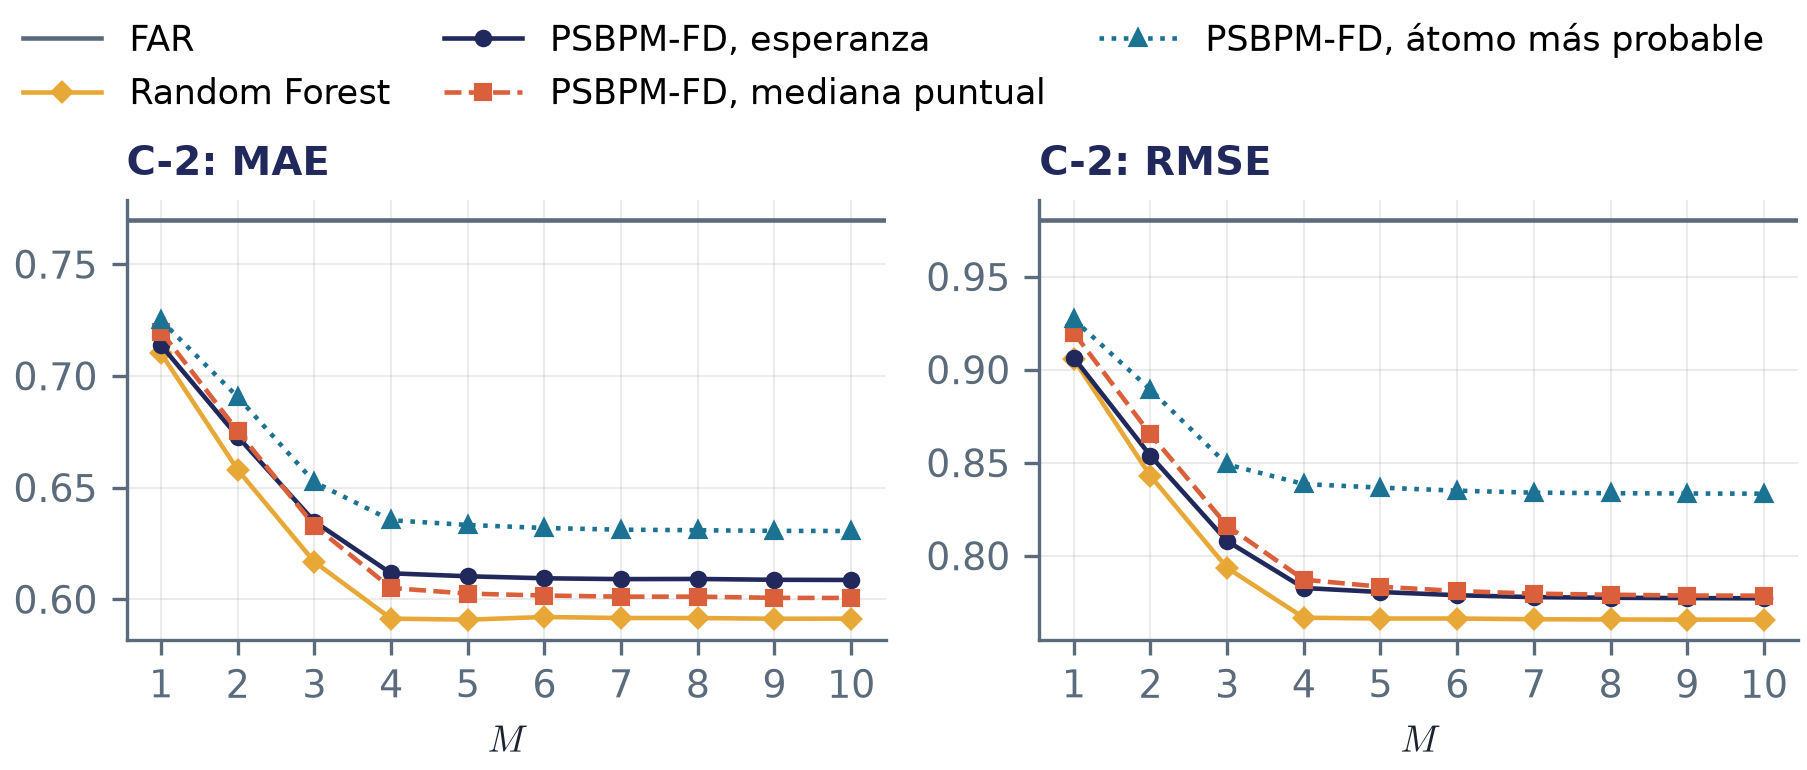
\includegraphics[width=\textwidth]{IMG/03_08/03_08_bloqueA_vs_M_C2.png}
\caption{C-2. MAE y RMSE en el bloque de prueba contra $M$.}
\label{fig:res_bloqueA_vs_M_C2}
\end{figure}

\begin{figure}[H]
\centering
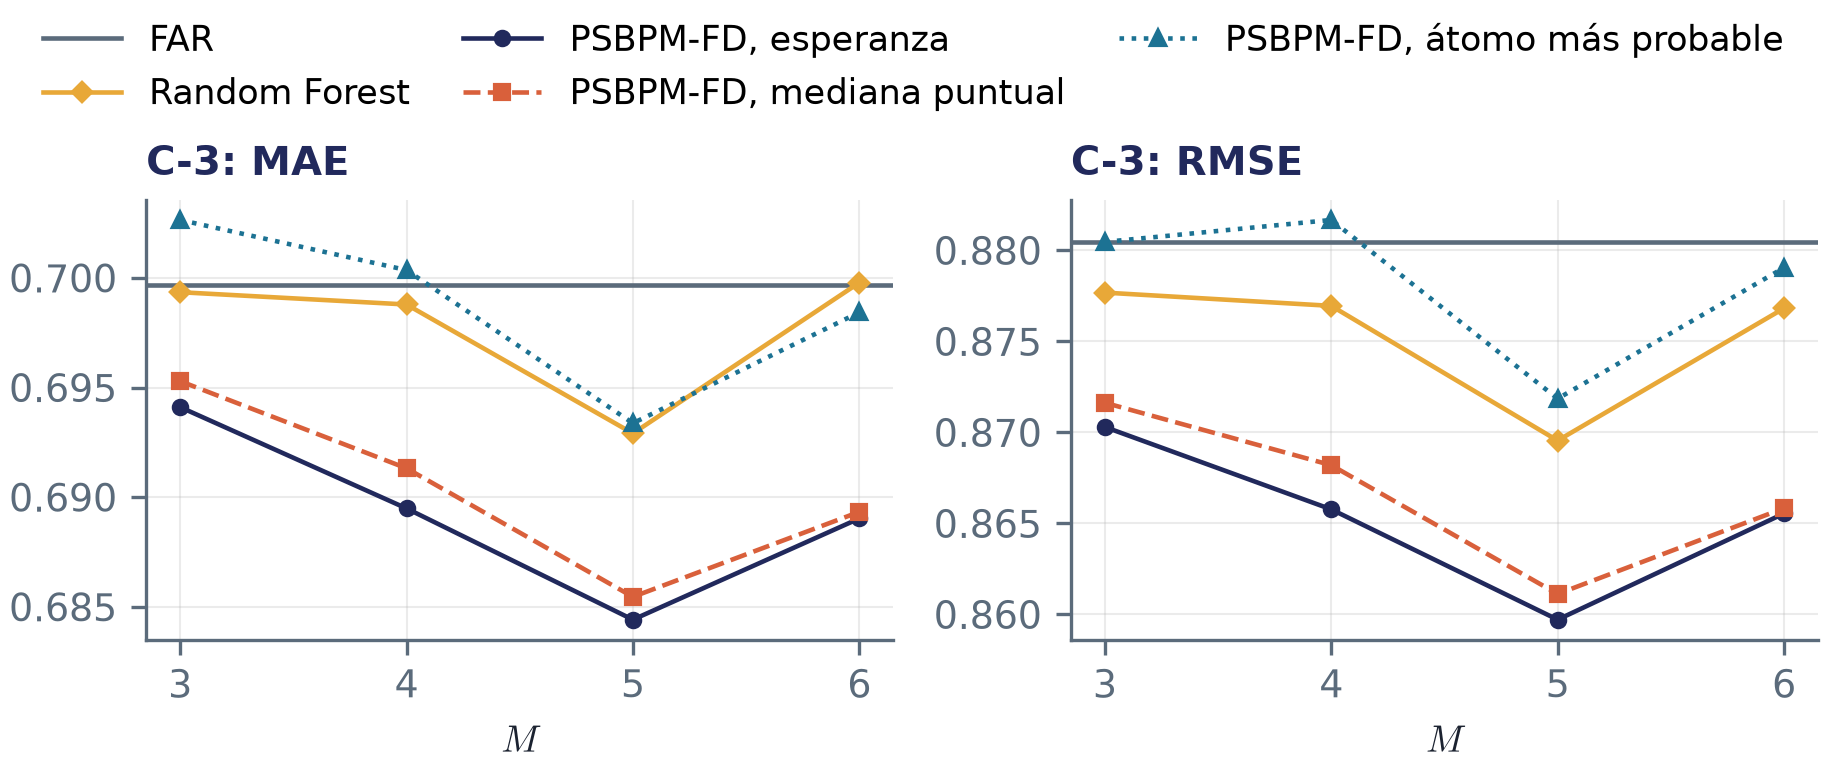
\includegraphics[width=\textwidth]{IMG/03_08/03_08_bloqueA_vs_M_C3.png}
\caption{C-3. MAE y RMSE en el bloque de prueba contra $M$.}
\label{fig:res_bloqueA_vs_M_C3}
\end{figure}
% Lectura M: el error decae hasta M = 4 (los J_a = 4 scores activos del generador) y después queda plano.
En las Figuras~\ref{fig:res_bloqueA_vs_M_C1} a~\ref{fig:res_bloqueA_vs_M_C3}, el error de todos los métodos que operan sobre los scores disminuye a medida que aumenta $M$, y lo hace de forma consistente en ambas métricas y en los tres escenarios. Se observa una caída pronunciada entre $M = 1$ y $M = 4$, seguida de un tramo plano en el que los valores solo varían en la tercera cifra. Esta caída se explica porque el error se mide contra la curva completa, por tanto la representación con $M$ scores omite la varianza de los $J - M$ restantes, y cada score adicional la recupera. El quiebre en $M = 4$ coincide con el diseño del generador. La dinámica de cada escenario reside en los $J_a = 4$ primeros scores, mientras que los seis restantes son autorregresivos débiles, casi impredecibles; incluirlos devuelve su varianza a la curva, pero no aporta información útil para la predicción. El FAR, que utiliza los $J$ coeficientes, sirve como referencia del truncamiento. Con $M \le 2$ gana en C-1 por construcción; la mezcla lo alcanza en $M = 3$ y lo supera desde $M = 4$. En C-2 lo supera ya con $M = 1$, porque el primer score concentra la mayor parte de la varianza y es el que más cambia de régimen. En C-3, donde las covariables son los rezagos de todos los scores y la dimensión del estado crece con $M$, el mínimo se alcanza en $M = 5$, mientras que $M = 6$ empeora, porque el sexto score es pasivo y lo que aporta como covariable a los pesos de la mezcla es ruido. El Random Forest sigue la misma trayectoria que el PSBPM-FD, ya que ve los mismos scores, y la distancia entre ambos se abre hasta $M = 4$ y después queda fija.

% Fuente: 98_resumen_bloqueA_min_max_prom.csv del _05 (test, M_ref); cambio relativo del promedio respecto del FAR.
\begin{table}[H]
\centering\footnotesize
\setlength{\tabcolsep}{4pt}
\caption{Cambio relativo del MAE y del RMSE respecto del FAR en $M_{\mathrm{ref}}$, por predictor y escenario. Negativo es mejor que el FAR.}
\label{tab:res_bloqueA_ganancia}
\begin{tabular}{l cc cc cc}
\hline
 & \multicolumn{2}{c}{C-1} & \multicolumn{2}{c}{C-2} & \multicolumn{2}{c}{C-3} \\
 & MAE & RMSE & MAE & RMSE & MAE & RMSE \\
\hline
PSBPM-FD, esperanza & $-1.7\%$ & $-1.7\%$ & $-20.9\%$ & $-20.7\%$ & $-1.5\%$ & $-1.7\%$ \\
PSBPM-FD, mediana puntual & $-1.6\%$ & $-1.6\%$ & $-22.0\%$ & $-20.6\%$ & $-1.5\%$ & $-1.7\%$ \\
PSBPM-FD, átomo más probable & $-0.9\%$ & $-0.6\%$ & $-18.1\%$ & $-15.0\%$ & $-0.2\%$ & $-0.2\%$ \\
Random Forest & $+1.5\%$ & $+1.6\%$ & $-23.2\%$ & $-21.9\%$ & $+0.0\%$ & $-0.4\%$ \\
\hline
\end{tabular}
\end{table}

% Lectura ganancia: el promedio dice cuánto se gana por estimador y en general.
El Cuadro~\ref{tab:res_bloqueA_ganancia} resume cuánto se gana en promedio respecto del FAR con cada estimador. En C-2 la ganancia es grande, en torno a un quinto del error en las dos métricas, y en C-1 y C-3 es pequeña, del orden del $2\%$. En los tres escenarios la esperanza y la mediana puntual ganan prácticamente lo mismo y el átomo más probable gana menos, porque se queda con un solo átomo por score y descarta la masa de los otros. La mediana puntual es el mejor estimador bajo MAE en C-2, donde la predictiva es bimodal en parte de los orígenes, y la esperanza lo es bajo RMSE en los tres escenarios, que es el reparto que corresponde a lo que cada métrica mide. El Random Forest, con las mismas covariables, gana más que el PSBPM-FD en C-2 y tiene un error mayor que el del FAR en C-1.

% Fuente: 72_ventana_modelos_w30.csv del _05 (test, M_ref, w = 30, sin el medoide); porcentaje de las 271 ventanas.
% Abajo: el predictor consistente con cada métrica (mediana puntual en C-2 y esperanza en C-1 y C-3 para el MAE; esperanza para el RMSE) contra cada referencia.
\begin{table}[H]
\centering\footnotesize
\caption{Ventanas de prueba ganadas en $M_{\mathrm{ref}}$. Arriba, fracción en que cada modelo es el mejor, abajo, fracción en que el predictor del PSBPM-FD supera a cada referencia.}
\label{tab:res_bloqueA_ventanas}
\begin{tabular}{l cc cc cc}
\hline
 & \multicolumn{2}{c}{C-1} & \multicolumn{2}{c}{C-2} & \multicolumn{2}{c}{C-3} \\
 & MAE & RMSE & MAE & RMSE & MAE & RMSE \\
\hline
FAR & 12\% & 7\% & 0\% & 0\% & 13\% & 7\% \\
Random Forest & 6\% & 3\% & 64\% & 60\% & 14\% & 15\% \\
PSBPM-FD, esperanza & 28\% & 56\% & 4\% & 21\% & 31\% & 36\% \\
PSBPM-FD, mediana puntual & 35\% & 25\% & 31\% & 19\% & 23\% & 30\% \\
PSBPM-FD, átomo más probable & 19\% & 9\% & 0\% & 0\% & 20\% & 11\% \\
\hline
PSBPM-FD gana al FAR & 87\% & 93\% & 100\% & 100\% & 85\% & 89\% \\
PSBPM-FD gana al Random Forest & 92\% & 96\% & 35\% & 31\% & 82\% & 83\% \\
\hline
\end{tabular}
\end{table}



% Lectura 2b: las ventanas. Una diferencia grande en el promedio se traduce en ganar casi todas las ventanas; una pequeña, en una mayoría.
Los promedios reflejan el comportamiento anteriormente descrito, porque los predictores puntuales del PSBPM-FD ganan la mayoría de las ventanas de prueba, cerca de nueve de cada diez frente al FAR y frente al Random Forest en C-1 y C-3, aunque ahí los promedios queden cerca, y todas las ventanas frente al FAR en C-2. La ventaja del Cuadro~\ref{tab:res_bloqueA_ganancia} no viene de un tramo particular del bloque de prueba sino que se repite a lo largo de él. Entre los predictores del PSBPM-FD el reparto sigue a la métrica, con la mediana puntual ganando más ventanas bajo MAE y la esperanza bajo RMSE, y el Random Forest gana dos de cada tres ventanas en C-2 por lo mismo que gana el promedio.


\begin{figure}[H]
\centering
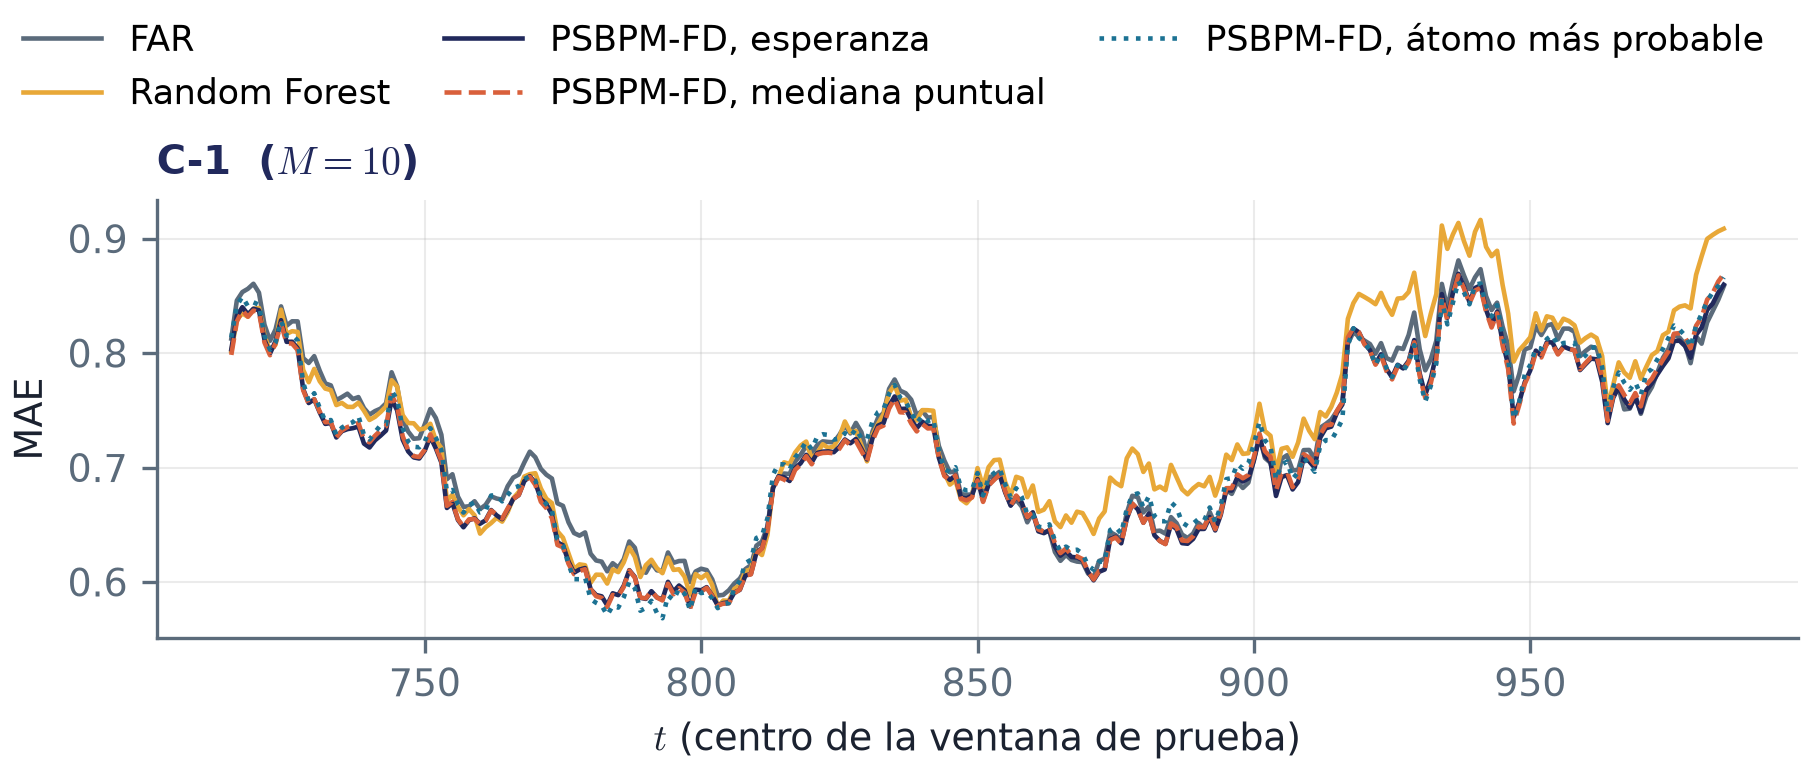
\includegraphics[width=\textwidth]{IMG/03_08/03_08_bloqueA_ventana_w30_C1.png}
\caption{C-1. MAE sobre la ventana móvil del bloque de prueba ($M_{\mathrm{ref}}$).}
\label{fig:res_bloqueA_ventana_C1}
\end{figure}

\begin{figure}[H]
\centering
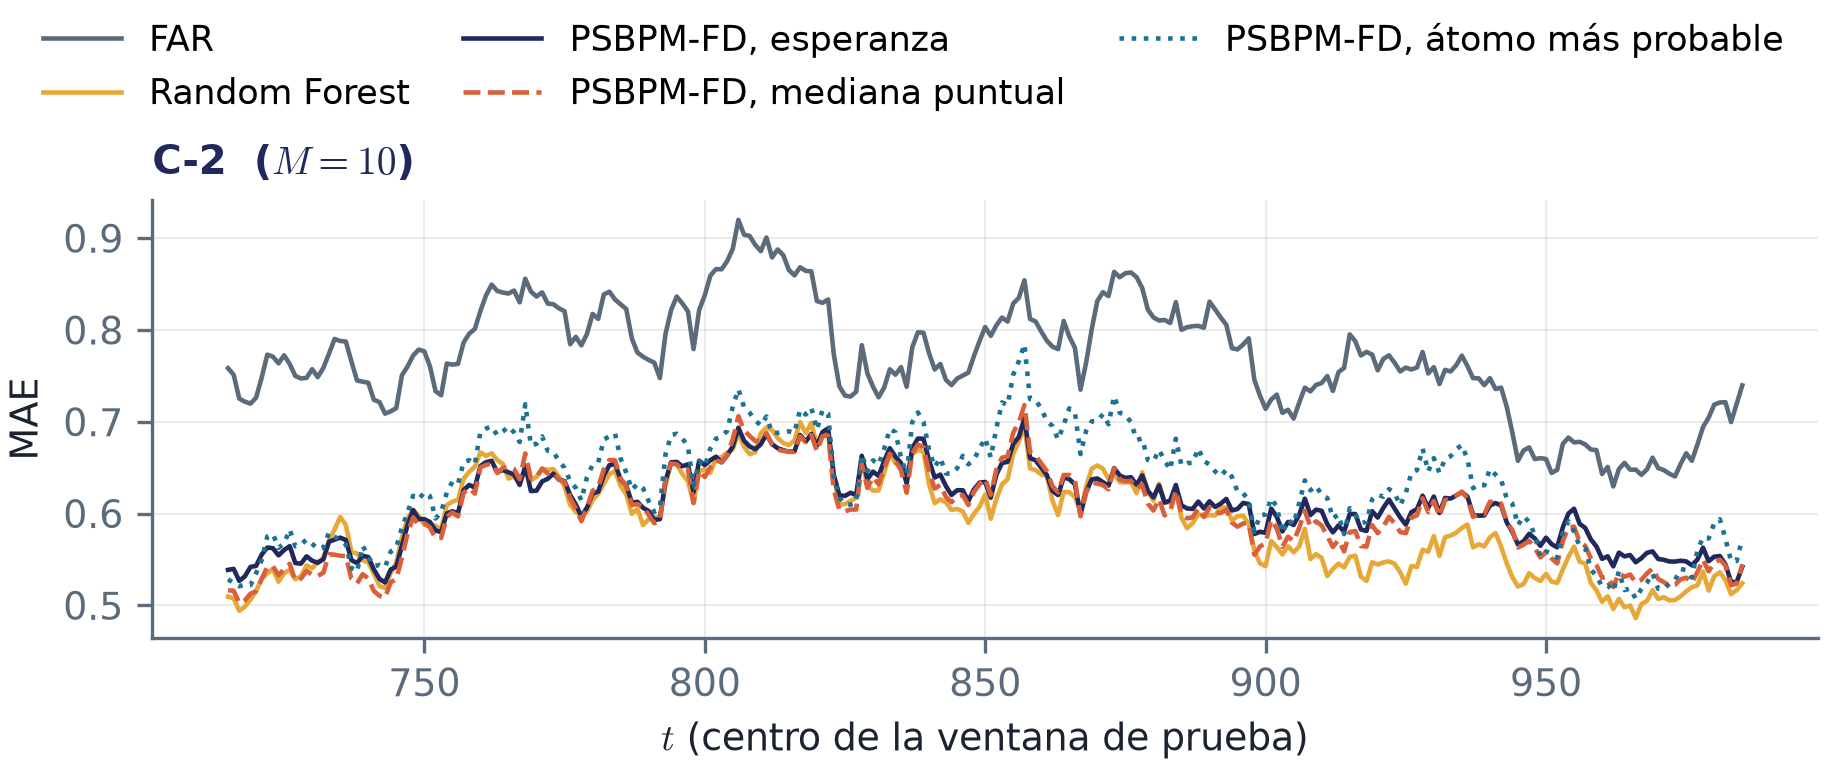
\includegraphics[width=\textwidth]{IMG/03_08/03_08_bloqueA_ventana_w30_C2.png}
\caption{C-2. MAE sobre la ventana móvil del bloque de prueba ($M_{\mathrm{ref}}$).}
\label{fig:res_bloqueA_ventana_C2}
\end{figure}

\begin{figure}[H]
\centering
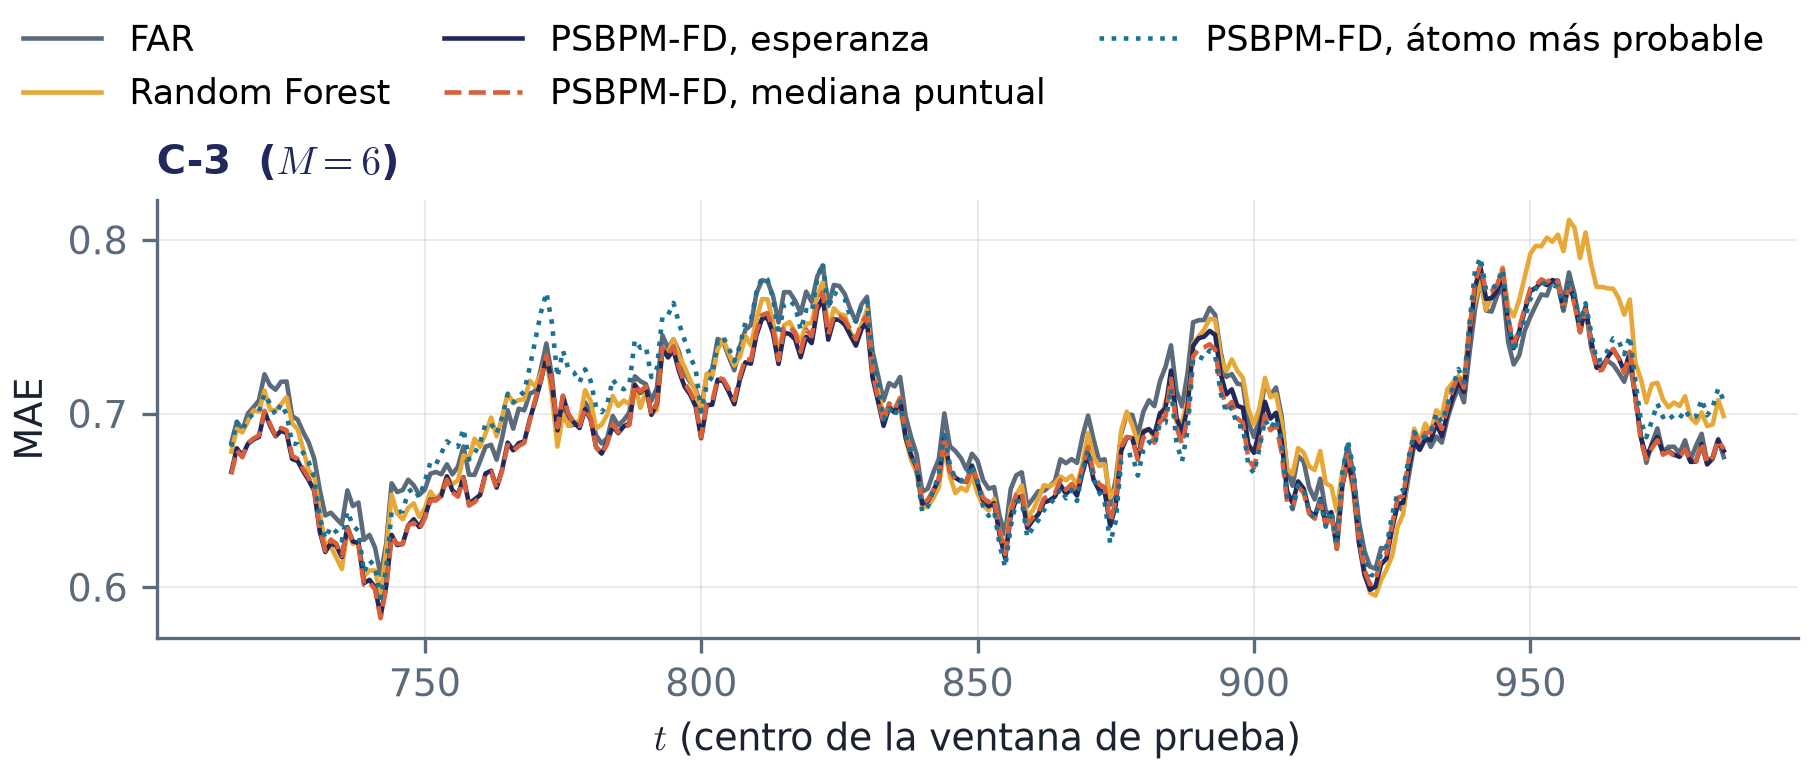
\includegraphics[width=\textwidth]{IMG/03_08/03_08_bloqueA_ventana_w30_C3.png}
\caption{C-3. MAE sobre la ventana móvil del bloque de prueba ($M_{\mathrm{ref}}$).}
\label{fig:res_bloqueA_ventana_C3}
\end{figure}
% Lectura 4: dónde gana a lo largo del test (tramos, no promedio).
Las Figuras~\ref{fig:res_bloqueA_ventana_C1} a~\ref{fig:res_bloqueA_ventana_C3} muestran que en C-2 la brecha con el FAR es uniforme, porque los regímenes cambian cada pocas curvas y toda ventana contiene ambos. En C-1 y C-3 todos los modelos suben y bajan juntos, porque el error está dominado por la innovación, que ningún modelo predice, y en C-1 su varianza cambia con el tiempo. Lo que distingue a los modelos es pequeño frente a eso, y se ve solo en los tramos tranquilos, donde el FAR queda por encima, y en el tramo final de C-1 y C-3, donde el Random Forest se despega hacia arriba.

\subsection{Intervalos de predicción}
\label{03_08_02_intervalos}

Los Cuadros~\ref{tab:res_bloqueB_por_M} a~\ref{tab:res_bloqueB_picp_por_M} resumen el Winkler, el MPIW y el PICP promedio sobre las ventanas de prueba, contra la curva ajustada, de las tres construcciones de intervalo del PSBPM-FD y de la banda gaussiana del FAR, para cada $M$ del barrido. Las Figuras~\ref{fig:res_bloqueB_vs_M_C1} a~\ref{fig:res_bloqueB_vs_M_C3} muestran las mismas cifras contra $M$, el Cuadro~\ref{tab:res_bloqueB_ganancia} cuánto cambia cada métrica respecto del FAR en $M_{\mathrm{ref}}$ y el Cuadro~\ref{tab:res_bloqueB_ventanas} cómo se reparten las ventanas entre las bandas.

% Fuente: 99_resumen_bloqueB_min_max_prom.csv del _05 (test, promedio sobre las ventanas, todas las bandas y M).
\begin{table}[H]
\centering\footnotesize
\setlength{\tabcolsep}{4pt}
\caption{Winkler en el bloque de prueba por escenario y $M$. En negrita el menor entre las construcciones en $M_{\mathrm{ref}}$, menor es mejor.}
\label{tab:res_bloqueB_por_M}
\begin{tabular}{c ccc ccc ccc}
\hline
 & \multicolumn{3}{c}{C-1} & \multicolumn{3}{c}{C-2} & \multicolumn{3}{c}{C-3} \\
$M$ & Equi-colas & HDR & Simult. & Equi-colas & HDR & Simult. & Equi-colas & HDR & Simult. \\
\hline
$1$ & 9.94 & 9.93 & 9.92 & 11.95 & 12.09 & 10.74 & --- & --- & --- \\
$2$ & 4.98 & 4.94 & 4.44 & 5.69 & 5.29 & 6.54 & --- & --- & --- \\
$3$ & 4.49 & 4.46 & 4.68 & 4.61 & 4.31 & 7.91 & 4.31 & 4.31 & 4.42 \\
$4$ & 4.32 & 4.30 & 4.92 & 3.97 & 3.75 & 6.73 & 4.15 & 4.16 & 4.71 \\
$5$ & 4.27 & 4.26 & 5.11 & 3.91 & 3.75 & 6.57 & 4.08 & 4.09 & 4.89 \\
$6$ & 4.24 & 4.24 & 5.19 & 3.90 & 3.76 & 6.32 & \textbf{4.11} & \textbf{4.11} & 4.99 \\
$7$ & 4.23 & 4.23 & 5.26 & 3.90 & 3.77 & 6.41 & --- & --- & --- \\
$8$ & 4.23 & 4.23 & 5.29 & 3.91 & 3.78 & 6.36 & --- & --- & --- \\
$9$ & 4.23 & 4.23 & 5.32 & 3.91 & 3.79 & 6.37 & --- & --- & --- \\
$10$ & \textbf{4.23} & \textbf{4.23} & 5.33 & 3.91 & \textbf{3.79} & 6.36 & --- & --- & --- \\
\hline
FAR & \multicolumn{3}{c}{4.35} & \multicolumn{3}{c}{4.86} & \multicolumn{3}{c}{4.23} \\
\hline
\end{tabular}
\end{table}

\begin{table}[H]
\centering\footnotesize
\setlength{\tabcolsep}{4pt}
\caption{MPIW en el bloque de prueba por escenario y $M$.}
\label{tab:res_bloqueB_mpiw_por_M}
\begin{tabular}{c ccc ccc ccc}
\hline
 & \multicolumn{3}{c}{C-1} & \multicolumn{3}{c}{C-2} & \multicolumn{3}{c}{C-3} \\
$M$ & Equi-colas & HDR & Simult. & Equi-colas & HDR & Simult. & Equi-colas & HDR & Simult. \\
\hline
$1$ & 1.95 & 1.95 & 1.96 & 1.76 & 1.46 & 2.01 & --- & --- & --- \\
$2$ & 2.82 & 2.82 & 3.70 & 2.79 & 2.56 & 6.08 & --- & --- & --- \\
$3$ & 3.09 & 3.10 & 4.39 & 3.14 & 2.97 & 7.79 & 2.98 & 2.98 & 4.16 \\
$4$ & 3.26 & 3.27 & 4.78 & 3.35 & 3.23 & 6.71 & 3.16 & 3.17 & 4.59 \\
$5$ & 3.37 & 3.37 & 5.01 & 3.45 & 3.35 & 6.55 & 3.26 & 3.27 & 4.80 \\
$6$ & 3.43 & 3.43 & 5.12 & 3.51 & 3.42 & 6.31 & 3.33 & 3.33 & 4.93 \\
$7$ & 3.45 & 3.46 & 5.19 & 3.54 & 3.45 & 6.40 & --- & --- & --- \\
$8$ & 3.47 & 3.48 & 5.23 & 3.56 & 3.47 & 6.34 & --- & --- & --- \\
$9$ & 3.48 & 3.49 & 5.25 & 3.57 & 3.49 & 6.35 & --- & --- & --- \\
$10$ & 3.49 & 3.49 & 5.26 & 3.58 & 3.49 & 6.35 & --- & --- & --- \\
\hline
FAR & \multicolumn{3}{c}{3.42} & \multicolumn{3}{c}{3.98} & \multicolumn{3}{c}{3.28} \\
\hline
\end{tabular}
\end{table}

\begin{table}[H]
\centering\footnotesize
\setlength{\tabcolsep}{4pt}
\caption{PICP en el bloque de prueba por escenario y $M$.}
\label{tab:res_bloqueB_picp_por_M}
\begin{tabular}{c ccc ccc ccc}
\hline
 & \multicolumn{3}{c}{C-1} & \multicolumn{3}{c}{C-2} & \multicolumn{3}{c}{C-3} \\
$M$ & Equi-colas & HDR & Simult. & Equi-colas & HDR & Simult. & Equi-colas & HDR & Simult. \\
\hline
$1$ & 0.640 & 0.640 & 0.641 & 0.541 & 0.493 & 0.604 & --- & --- & --- \\
$2$ & 0.869 & 0.872 & 0.953 & 0.817 & 0.813 & 0.968 & --- & --- & --- \\
$3$ & 0.910 & 0.911 & 0.979 & 0.891 & 0.899 & 0.992 & 0.908 & 0.910 & 0.980 \\
$4$ & 0.932 & 0.932 & 0.990 & 0.945 & 0.955 & 0.998 & 0.931 & 0.931 & 0.991 \\
$5$ & 0.939 & 0.942 & 0.993 & 0.957 & 0.965 & 0.999 & 0.943 & 0.942 & 0.993 \\
$6$ & 0.943 & 0.945 & 0.994 & 0.964 & 0.971 & 0.999 & 0.944 & 0.945 & 0.995 \\
$7$ & 0.945 & 0.947 & 0.995 & 0.967 & 0.974 & 0.999 & --- & --- & --- \\
$8$ & 0.946 & 0.948 & 0.995 & 0.968 & 0.974 & 0.999 & --- & --- & --- \\
$9$ & 0.946 & 0.948 & 0.995 & 0.968 & 0.975 & 0.999 & --- & --- & --- \\
$10$ & 0.947 & 0.948 & 0.995 & 0.969 & 0.975 & 0.999 & --- & --- & --- \\
\hline
FAR & \multicolumn{3}{c}{0.940} & \multicolumn{3}{c}{0.952} & \multicolumn{3}{c}{0.937} \\
\hline
\end{tabular}
\end{table}

% Figura Bloque B contra M: Winkler, MPIW y PICP de las tres construcciones y del FAR. Fuente: 99_* del _05.
\begin{figure}[H]
\centering
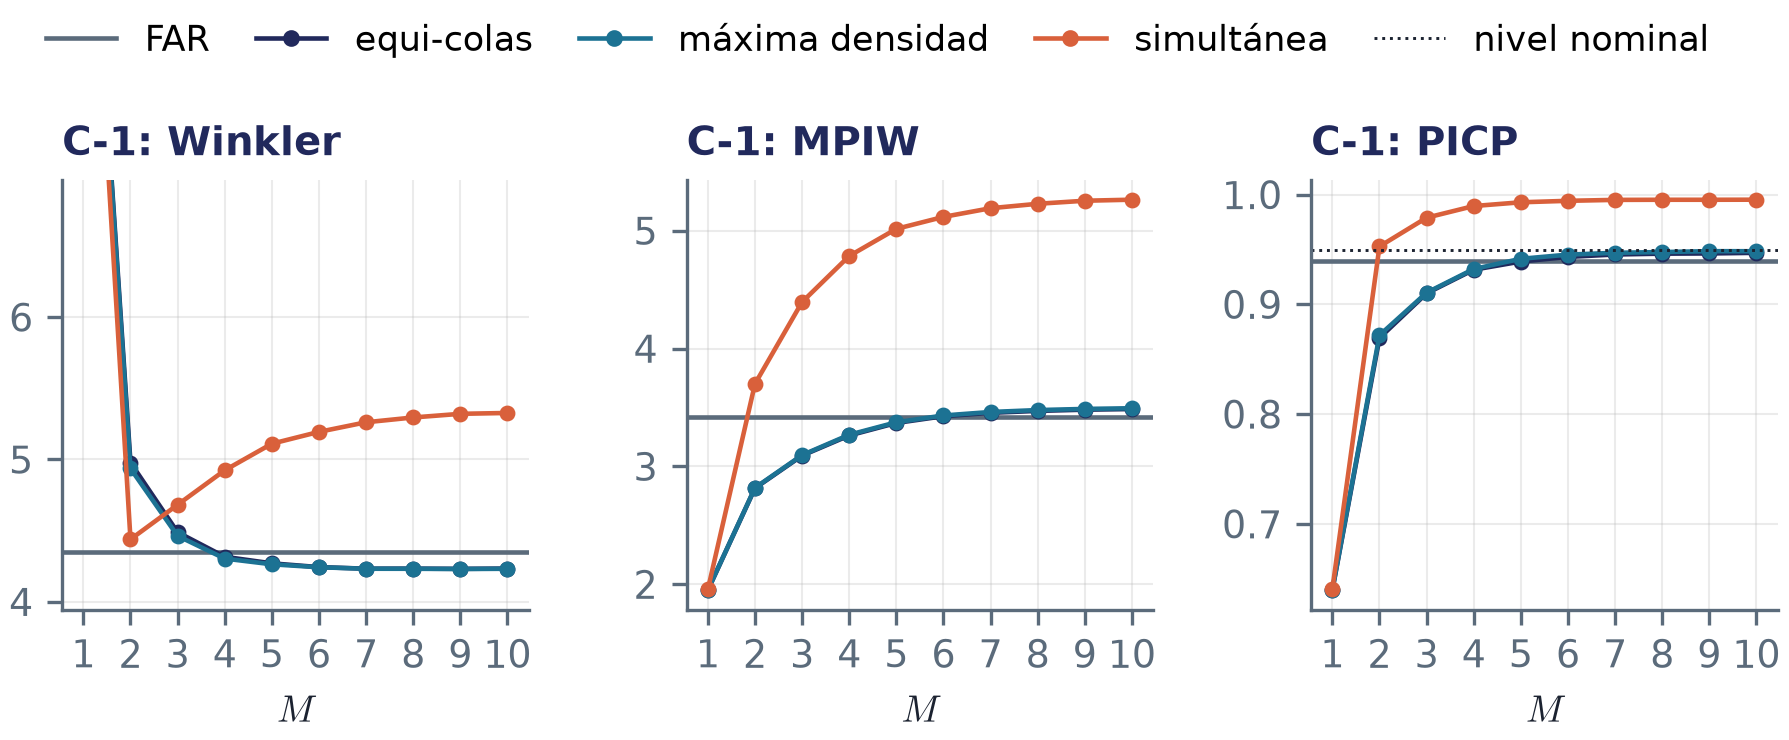
\includegraphics[width=\textwidth]{IMG/03_08/03_08_bloqueB_vs_M_C1.png}
\caption{C-1. Winkler, MPIW y PICP en el bloque de prueba contra $M$. El eje del Winkler se corta para que $M = 1$ no aplaste el resto.}
\label{fig:res_bloqueB_vs_M_C1}
\end{figure}

\begin{figure}[H]
\centering
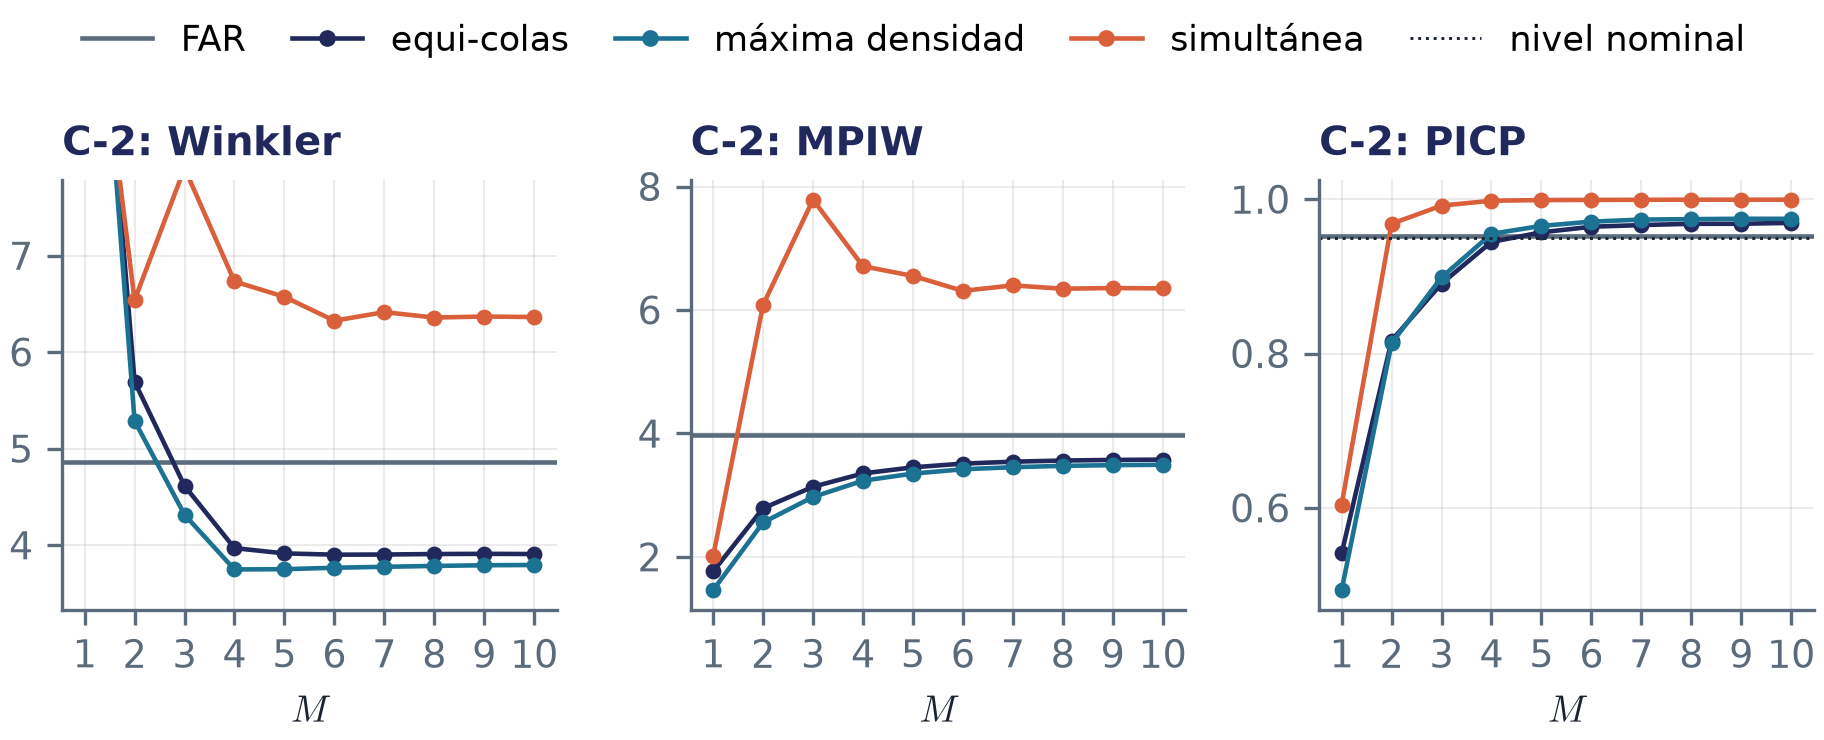
\includegraphics[width=\textwidth]{IMG/03_08/03_08_bloqueB_vs_M_C2.png}
\caption{C-2. Winkler, MPIW y PICP en el bloque de prueba contra $M$. El eje del Winkler se corta para que $M = 1$ no aplaste el resto.}
\label{fig:res_bloqueB_vs_M_C2}
\end{figure}

\begin{figure}[H]
\centering
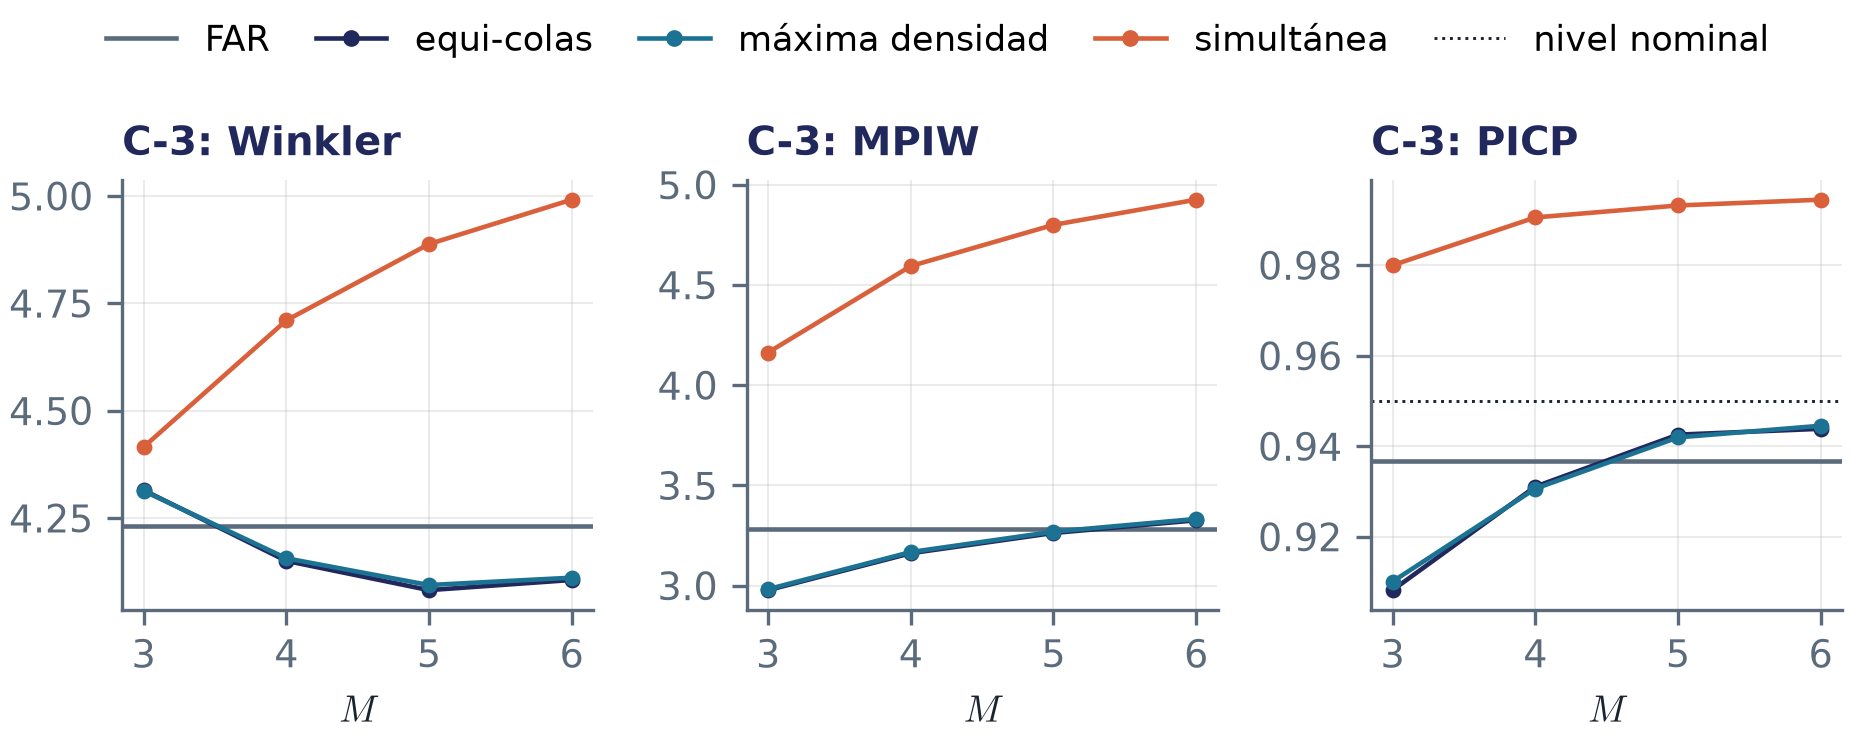
\includegraphics[width=\textwidth]{IMG/03_08/03_08_bloqueB_vs_M_C3.png}
\caption{C-3. Winkler, MPIW y PICP en el bloque de prueba contra $M$. El eje del Winkler se corta para que $M = 1$ no aplaste el resto.}
\label{fig:res_bloqueB_vs_M_C3}
\end{figure}

% Lectura M: las bandas mejoran hasta M = 4 por la misma razón que el error puntual, y la simultánea es la única que sigue ensanchándose.
En las Figuras~\ref{fig:res_bloqueB_vs_M_C1} a~\ref{fig:res_bloqueB_vs_M_C3} las tres métricas se mueven con $M$ de la misma forma en los tres escenarios. Con $M = 1$ la banda cubre solo la variabilidad del primer score y deja fuera la de los demás, que sí están en la curva contra la que se mide, por eso es angosta, su PICP queda muy por debajo del nominal y su Winkler es más del doble del FAR. Cada score que entra agrega su dispersión a la banda, el MPIW crece, el PICP sube hacia el nominal y el Winkler baja, y desde $M = 4$ las tres quedan planas, igual que el error puntual y por la misma razón, porque los seis scores restantes son pasivos. Las bandas puntuales, equi-colas y máxima densidad, se estabilizan en un PICP cercano al nominal con un ancho parecido al del FAR. En C-1 y C-3 la simultánea es la única que sigue ensanchándose con $M$, porque debe contener la curva entera y el supremo sobre el dominio crece con cada score que se agrega aunque este aporte poco a cada punto; en C-2 su ancho baja desde $M = 3$. Solo es la mejor de las tres con $M \le 2$ en C-1 y con $M = 1$ en C-2, cuando las otras dos todavía quedan cortas.

% Fuente: 99_resumen_bloqueB_min_max_prom.csv del _05 (test, M_ref); cambio relativo del promedio respecto del FAR.
\begin{table}[H]
\centering\small
\caption{Cambio relativo del Winkler, el MPIW y el PICP respecto del FAR en $M_{\mathrm{ref}}$, por escenario y construcción. En el Winkler y el MPIW negativo es mejor que el FAR, en el PICP positivo es más cobertura.}
\label{tab:res_bloqueB_ganancia}
\begin{tabular}{l l ccc}
\hline
Escenario & Banda & Winkler & MPIW & PICP \\
\hline
C-1 & Equi-colas & $-2.7\%$ & $+1.9\%$ & $+0.7\%$ \\
 & Máxima densidad & $-2.8\%$ & $+2.1\%$ & $+0.9\%$ \\
 & Simultánea & $+22.4\%$ & $+53.7\%$ & $+5.9\%$ \\
\hline
C-2 & Equi-colas & $-19.7\%$ & $-10.1\%$ & $+1.8\%$ \\
 & Máxima densidad & $-22.0\%$ & $-12.2\%$ & $+2.4\%$ \\
 & Simultánea & $+30.8\%$ & $+59.7\%$ & $+5.0\%$ \\
\hline
C-3 & Equi-colas & $-3.0\%$ & $+1.3\%$ & $+0.8\%$ \\
 & Máxima densidad & $-2.8\%$ & $+1.5\%$ & $+0.8\%$ \\
 & Simultánea & $+18.0\%$ & $+50.0\%$ & $+6.2\%$ \\
\hline
\end{tabular}
\end{table}

% Lectura ganancia: cuánto se gana por construcción y de dónde viene (ancho o cobertura).
El Cuadro~\ref{tab:res_bloqueB_ganancia} dice cuánto se gana respecto del FAR con cada construcción y de dónde viene la ganancia, porque el Winkler suma el ancho y una penalización por los puntos no cubiertos. En C-2 las bandas puntuales bajan el Winkler en un quinto y lo hacen por las dos vías a la vez, una banda un $10\%$ más angosta que además cubre más. Eso solo es posible porque el ancho de la banda del PSBPM-FD sigue el régimen en que está cada score, mientras que el del FAR hereda una varianza residual fija y es el mismo en todos los orígenes. En C-1 y C-3 la ganancia es del orden del $3\%$ y tiene otra composición, la banda del PSBPM-FD es apenas más ancha y su PICP queda más cerca del nominal, de modo que gana por calibración y no por ancho. Esa ganancia pequeña se explica igual que en el error puntual, la referencia gaussiana está casi bien especificada cuando la media es lineal y la varianza cambia poco. La máxima densidad coincide con la equi-colas en C-1 y C-3, porque con una predictiva unimodal y simétrica ambas son el mismo intervalo central, y solo en C-2 la mejora, reasignando a los modos la masa que la equi-colas gasta en el valle entre ellos. La simultánea pierde el Winkler en los tres escenarios porque es entre $1.5$ y $1.6$ veces más ancha, que es lo que cuesta contener la curva entera y no cada punto por separado, y es la única construcción calibrada para esa cobertura. Queda por ver si estos promedios reflejan el comportamiento a lo largo del bloque de prueba.

% Fuente: 81_ventana_bloqueB_w30.csv del _05 (test, M_ref, w = 30); porcentaje de las 271 ventanas, por Winkler.
\begin{table}[H]
\centering\small
\caption{Ventanas de prueba ganadas en $M_{\mathrm{ref}}$ por Winkler. Arriba, fracción en que cada banda es la mejor, abajo, fracción en que cada construcción del PSBPM-FD supera al FAR.}
\label{tab:res_bloqueB_ventanas}
\begin{tabular}{l ccc}
\hline
 & C-1 & C-2 & C-3 \\
\hline
FAR & 11\% & 0\% & 18\% \\
Equi-colas & 35\% & 9\% & 46\% \\
Máxima densidad & 54\% & 91\% & 36\% \\
Simultánea & 0\% & 0\% & 0\% \\
\hline
Equi-colas gana al FAR & 81\% & 100\% & 81\% \\
Máxima densidad gana al FAR & 88\% & 100\% & 73\% \\
Simultánea gana al FAR & 5\% & 0\% & 1\% \\
\hline
\end{tabular}
\end{table}

% Lectura ventanas: los promedios reflejan el comportamiento.
 Las bandas puntuales del PSBPM-FD ganan al FAR en todas las ventanas de C-2 y en cuatro de cada cinco de C-1 y C-3, aunque ahí los promedios queden a un $3\%$, de modo que la ventaja se repite a lo largo del bloque de prueba y no viene de unos pocos tramos. Entre las construcciones, la máxima densidad es la mejor en nueve de cada diez ventanas de C-2, donde la predictiva tiene valles, y en C-1 y C-3 se reparte con la equi-colas porque son casi la misma banda. La simultánea no gana ninguna ventana por Winkler, que es lo esperable de una banda que ensancha el intervalo.

% Figura: Winkler sobre la ventana móvil de prueba, w_ref, M_ref. Fuente: 81_ventana_bloqueB_w30.csv del _05.
\begin{figure}[H]
\centering
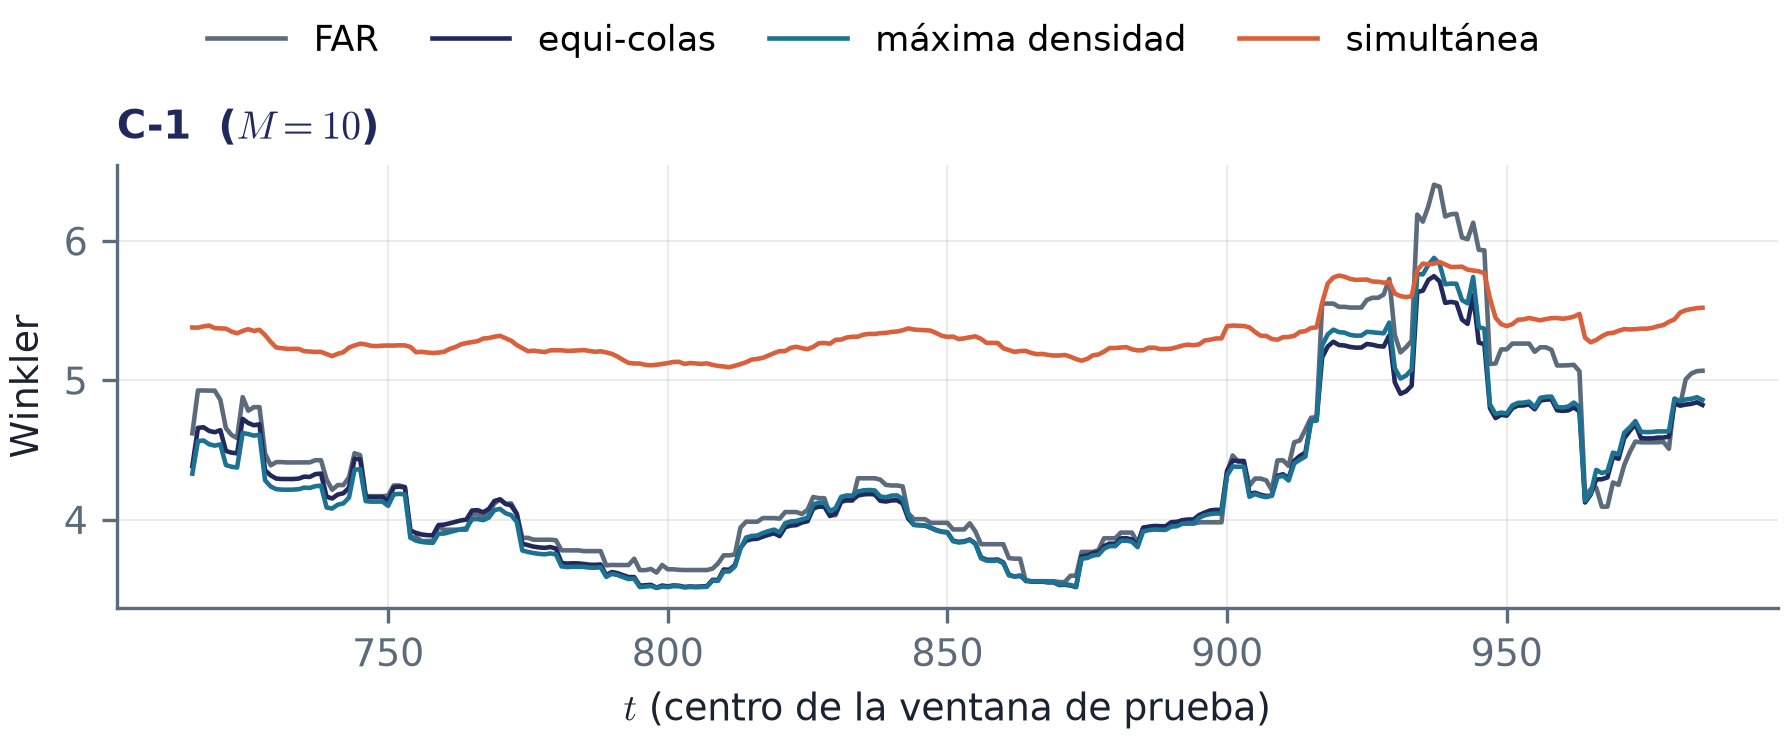
\includegraphics[width=\textwidth]{IMG/03_08/03_08_bloqueB_ventana_w30_C1.png}
\caption{C-1. Winkler sobre la ventana móvil del bloque de prueba ($M_{\mathrm{ref}}$).}
\label{fig:res_bloqueB_ventana_C1}
\end{figure}

\begin{figure}[H]
\centering
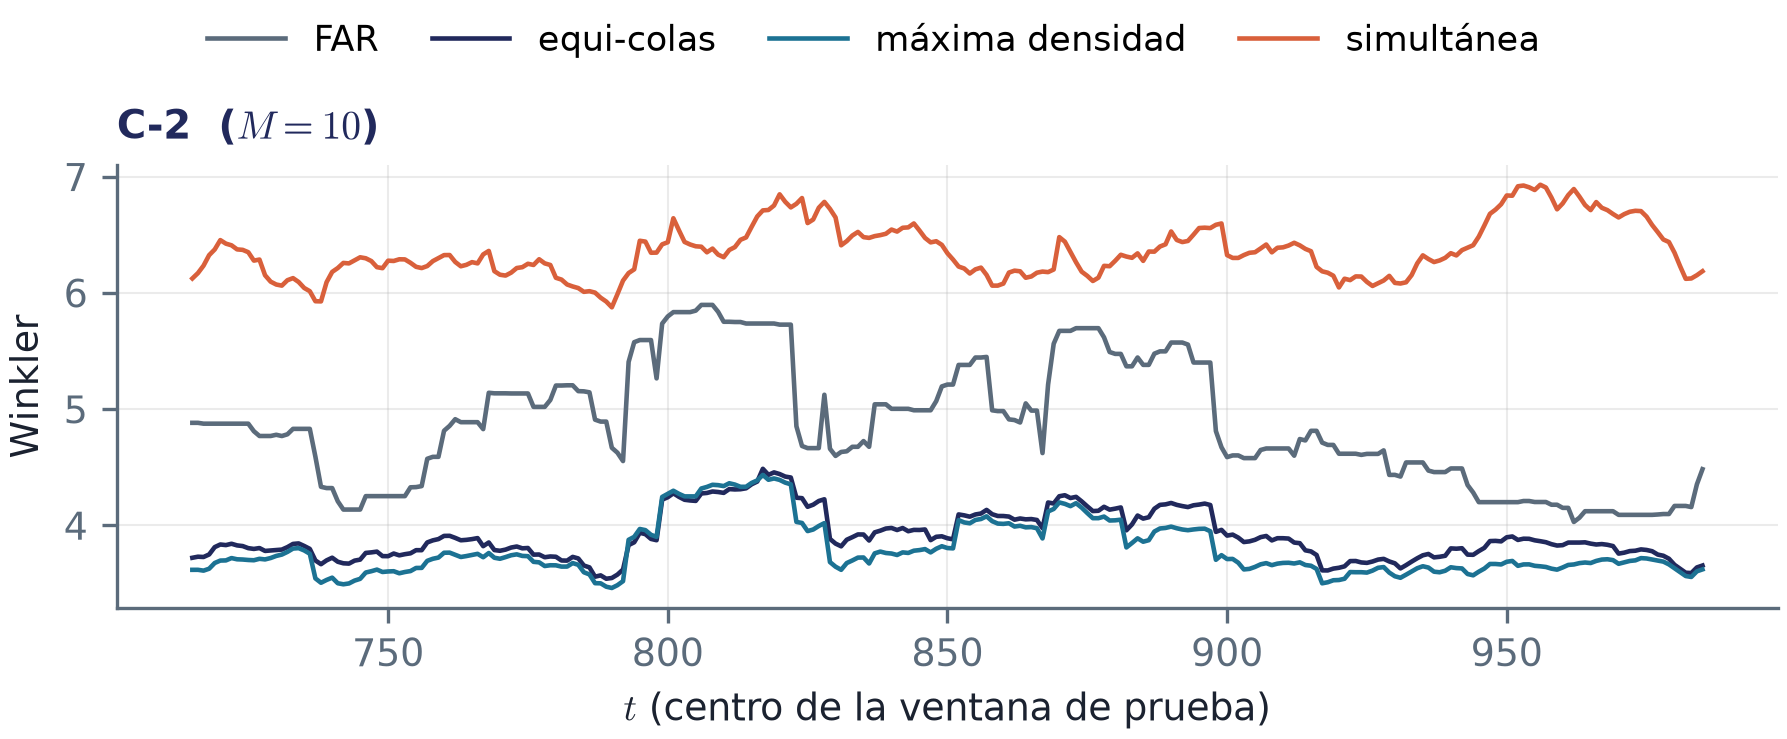
\includegraphics[width=\textwidth]{IMG/03_08/03_08_bloqueB_ventana_w30_C2.png}
\caption{C-2. Winkler sobre la ventana móvil del bloque de prueba ($M_{\mathrm{ref}}$).}
\label{fig:res_bloqueB_ventana_C2}
\end{figure}

\begin{figure}[H]
\centering
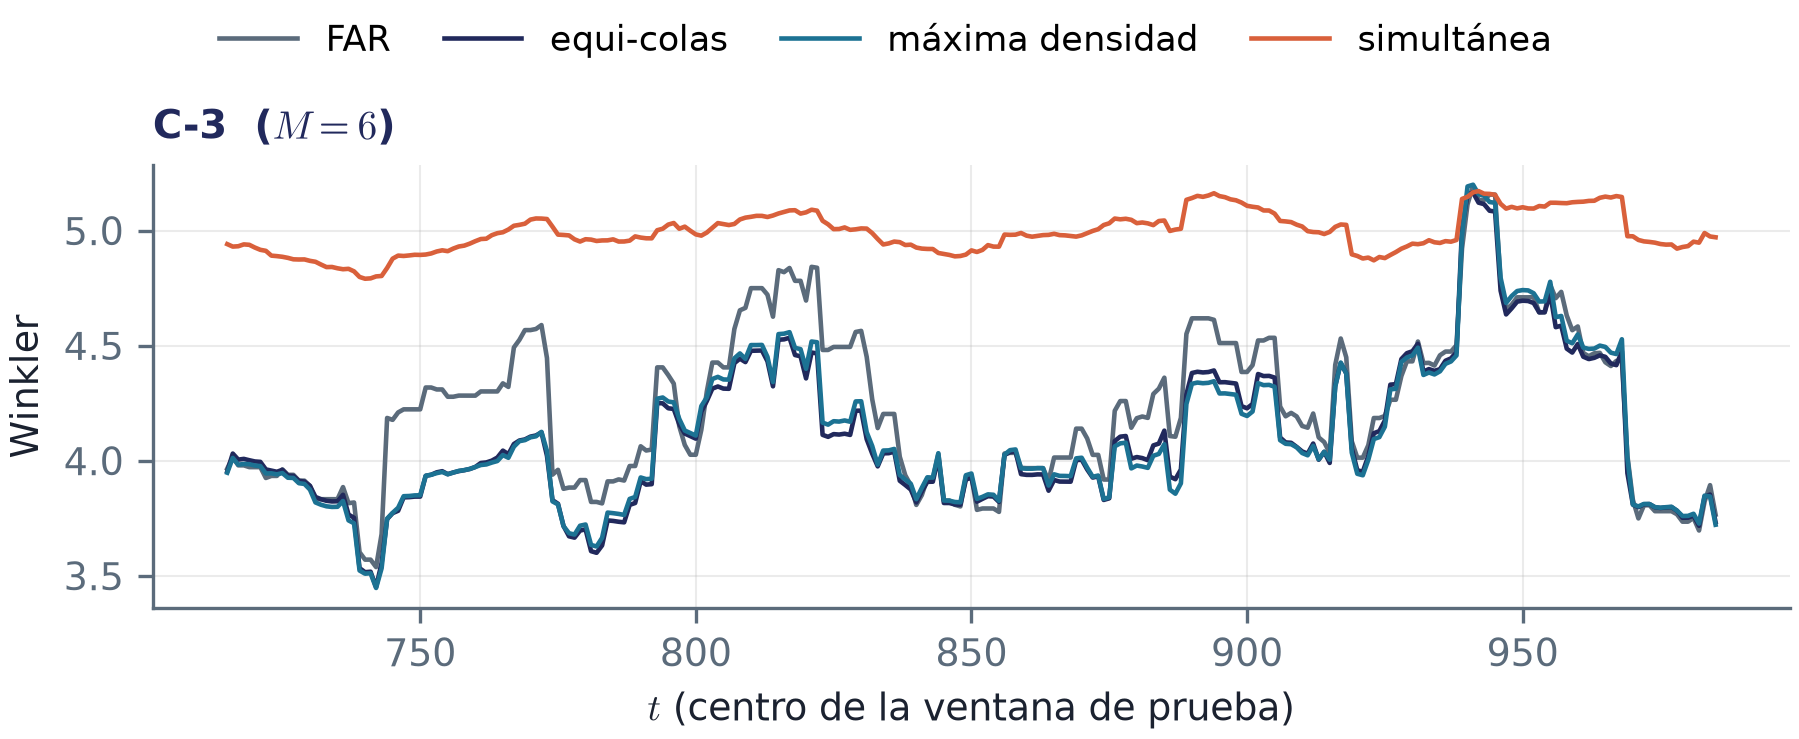
\includegraphics[width=\textwidth]{IMG/03_08/03_08_bloqueB_ventana_w30_C3.png}
\caption{C-3. Winkler sobre la ventana móvil del bloque de prueba ($M_{\mathrm{ref}}$).}
\label{fig:res_bloqueB_ventana_C3}
\end{figure}

% Lectura trayectoria: el ancho del FAR no depende del origen y el del PSBPM-FD sí. Ésa es la diferencia clave.
Las Figuras~\ref{fig:res_bloqueB_ventana_C1} a~\ref{fig:res_bloqueB_ventana_C3} muestran de dónde sale la diferencia. Con una cantidad suficiente de componentes para contener la dinámica, el PSBPM-FD adapta el ancho de su banda al estado del proceso en cada origen, mientras que la banda del FAR tiene el mismo ancho en todos los orígenes y su Winkler solo se mueve por la penalización de los puntos que deja fuera. Por eso en C-2 el Winkler del FAR sube cada vez que la ventana contiene episodios del régimen volátil y el del PSBPM-FD se mantiene estable y por debajo en todas las ventanas, porque la banda se ensancha en esos episodios y se angosta en los tranquilos. En C-1 las curvas suben juntas en el episodio de volatilidad del tramo final, alrededor de $t = 930$, donde la banda del PSBPM-FD se ensancha y acompaña al proceso, y la ventaja aparece en los tramos tranquilos, donde la banda gaussiana es más ancha de lo necesario. En C-3 las curvas se superponen y el FAR se despega hacia arriba en las ventanas con los peores errores. El modelo no es conservador por regla, es angosto donde el proceso está tranquilo y ancho donde cambia de régimen, y esa es la diferencia que una banda de ancho fijo no puede dar. Las Figuras~\ref{fig:res_bloqueB_ancho_C1} a~\ref{fig:res_bloqueB_ancho_C3} lo muestran de forma directa con el ancho medio de la banda en cada origen de prueba. El del FAR es una línea horizontal y el del PSBPM-FD se mueve con el estado del proceso, por debajo del FAR en los tramos tranquilos y por encima en los episodios en que la varianza condicional sube, en C-1, o en que algún score está en el régimen volátil, en C-2. En C-3 el ancho también cambia de origen en origen, aunque con menos amplitud, porque la dispersión de la mezcla depende de los rezagos aun cuando la media condicional sea casi lineal.

% Figura: ancho medio de la banda por origen de prueba. Fuente: banda_funcional_psbp.npz del _04 (li, ls, hdr_L, hdr_U, li/ls_simultanea) y el MPIW del FAR de 81_*.
\begin{figure}[H]
\centering
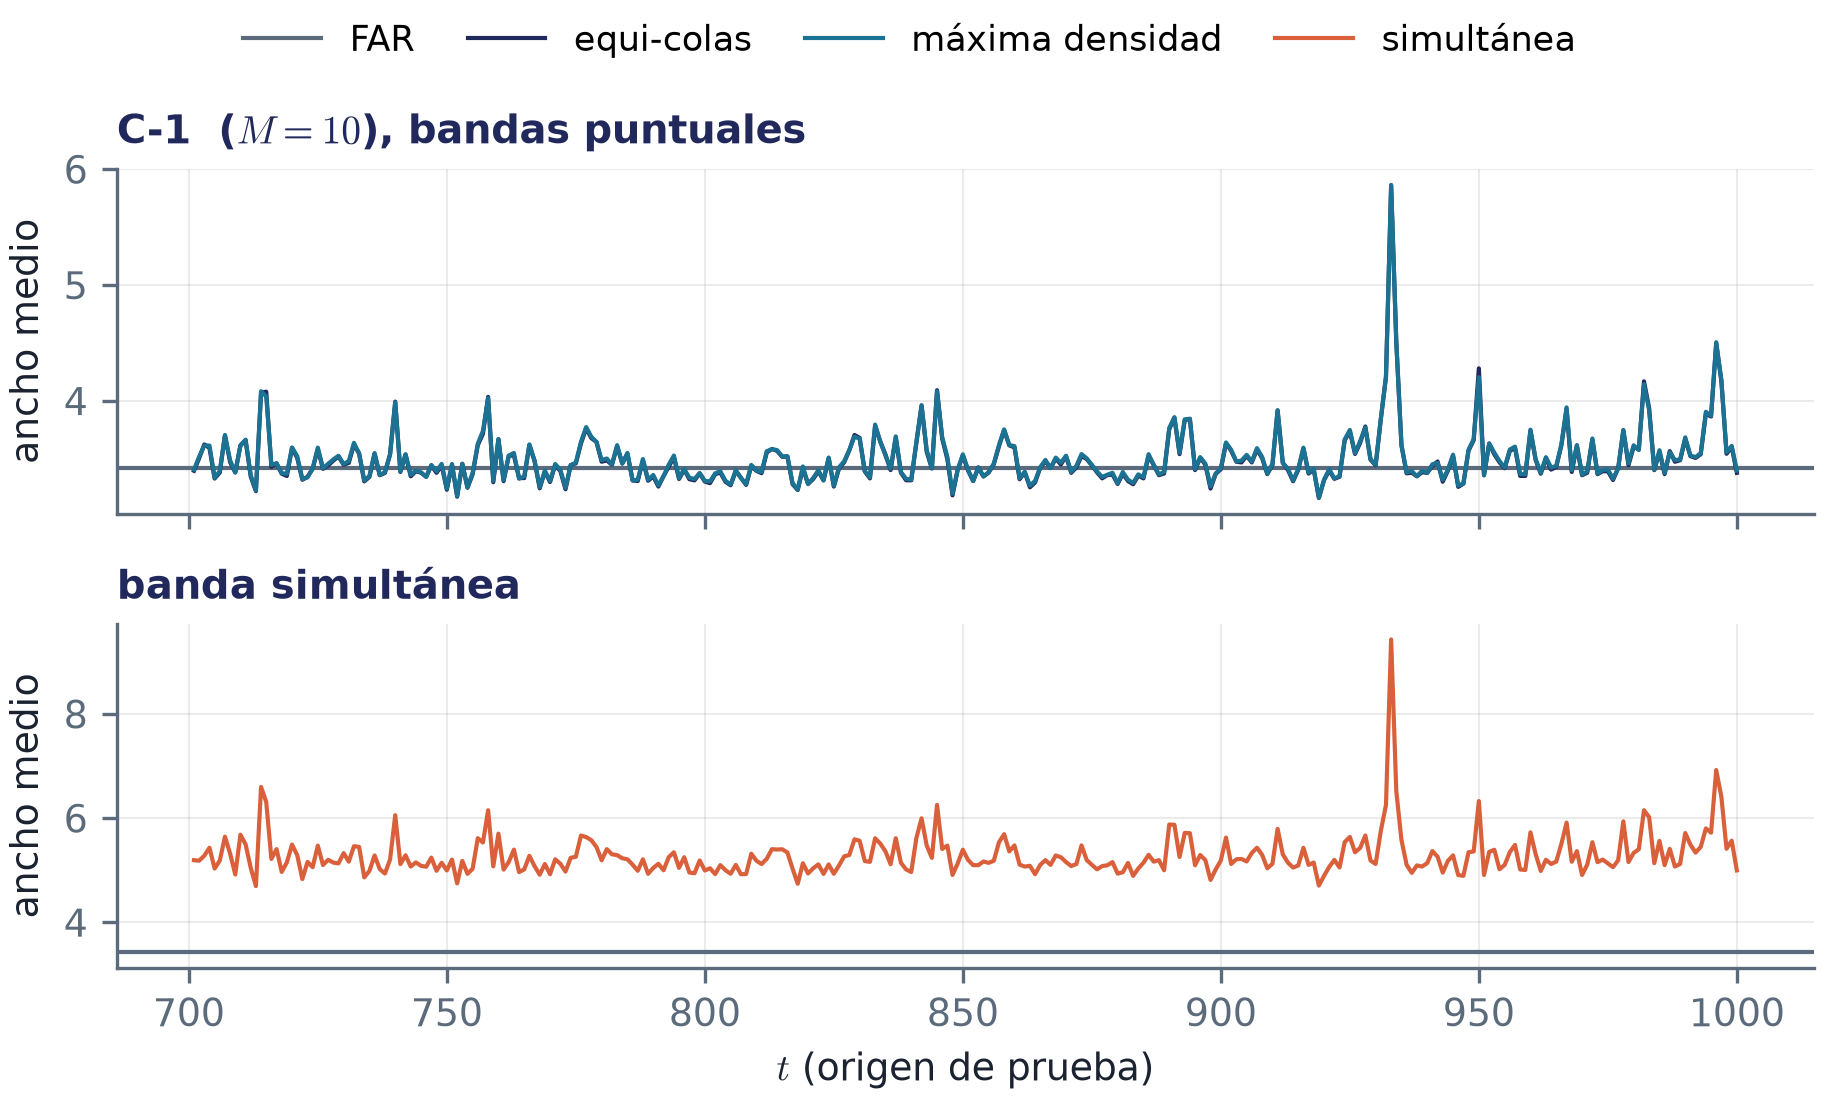
\includegraphics[width=\textwidth]{IMG/03_08/03_08_bloqueB_ancho_C1.png}
\caption{C-1. Ancho medio de la banda en cada origen de prueba ($M_{\mathrm{ref}}$) de las tres construcciones del PSBPM-FD y ancho fijo del FAR.}
\label{fig:res_bloqueB_ancho_C1}
\end{figure}

\begin{figure}[H]
\centering
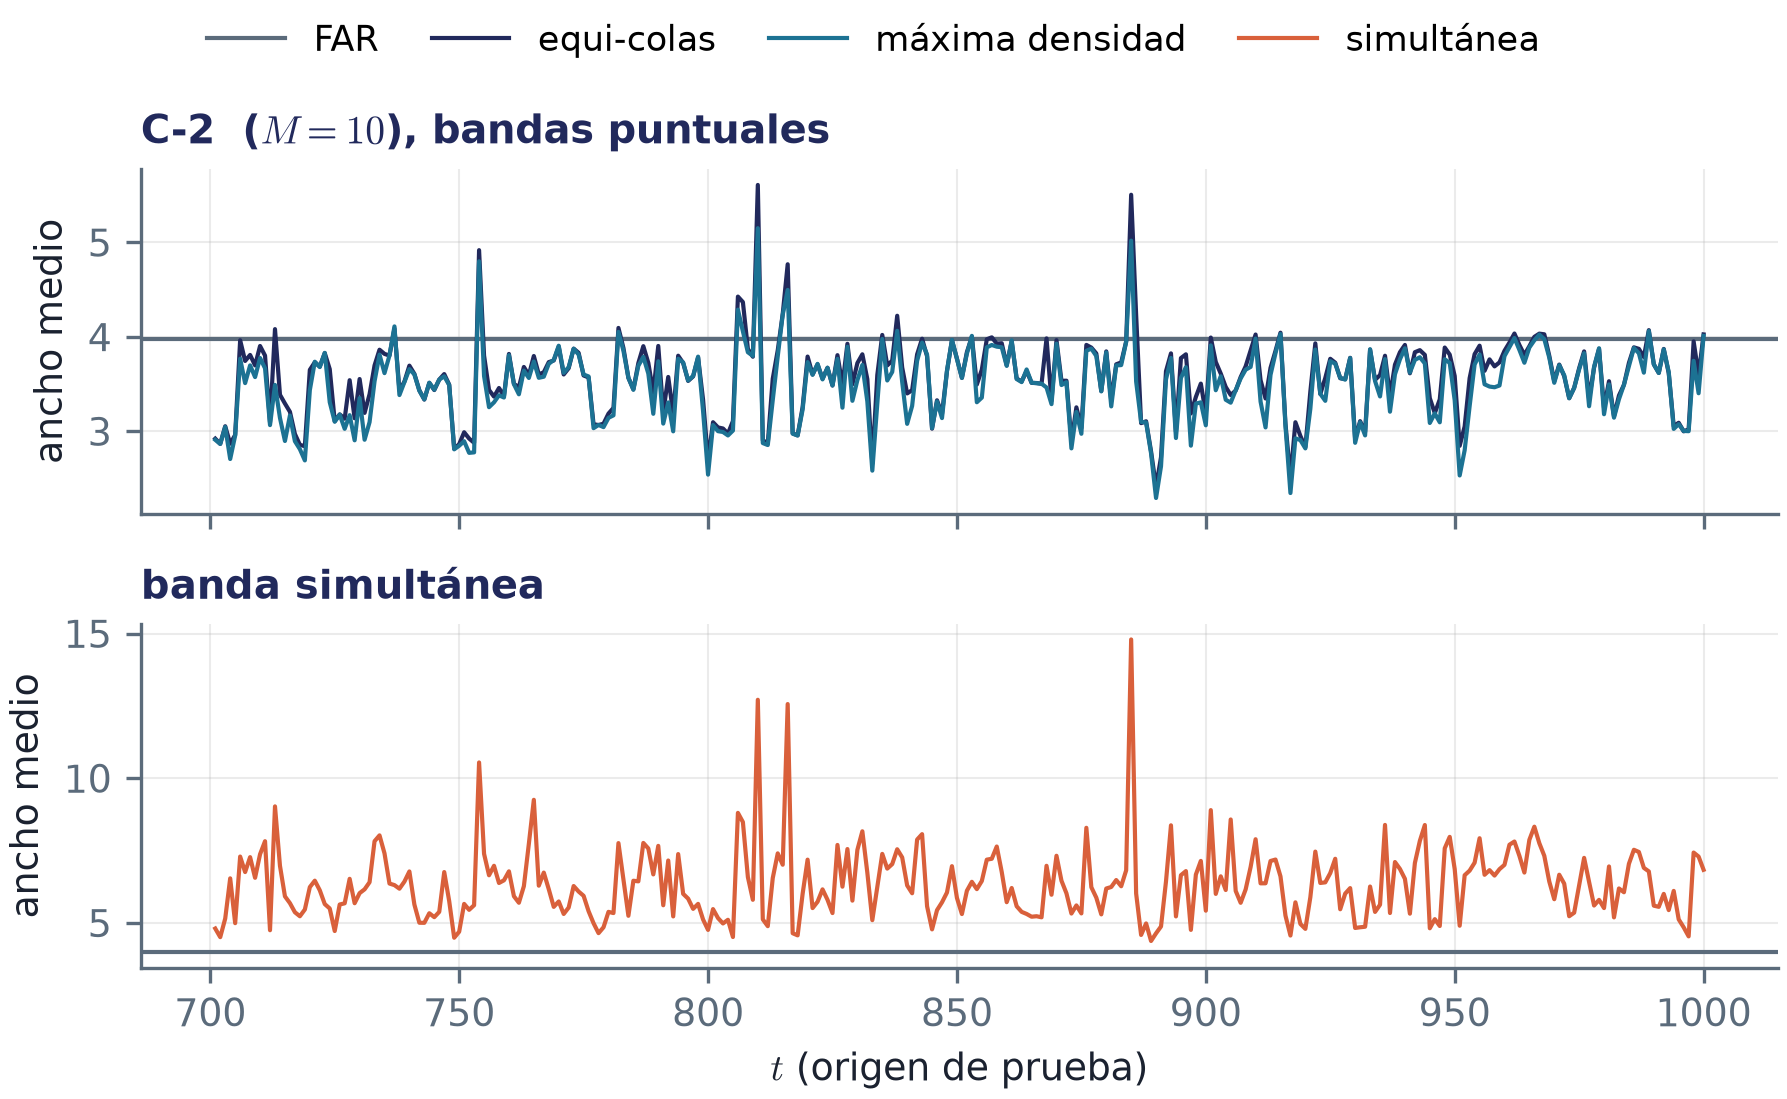
\includegraphics[width=\textwidth]{IMG/03_08/03_08_bloqueB_ancho_C2.png}
\caption{C-2. Ancho medio de la banda en cada origen de prueba ($M_{\mathrm{ref}}$) de las tres construcciones del PSBPM-FD y ancho fijo del FAR.}
\label{fig:res_bloqueB_ancho_C2}
\end{figure}

\begin{figure}[H]
\centering
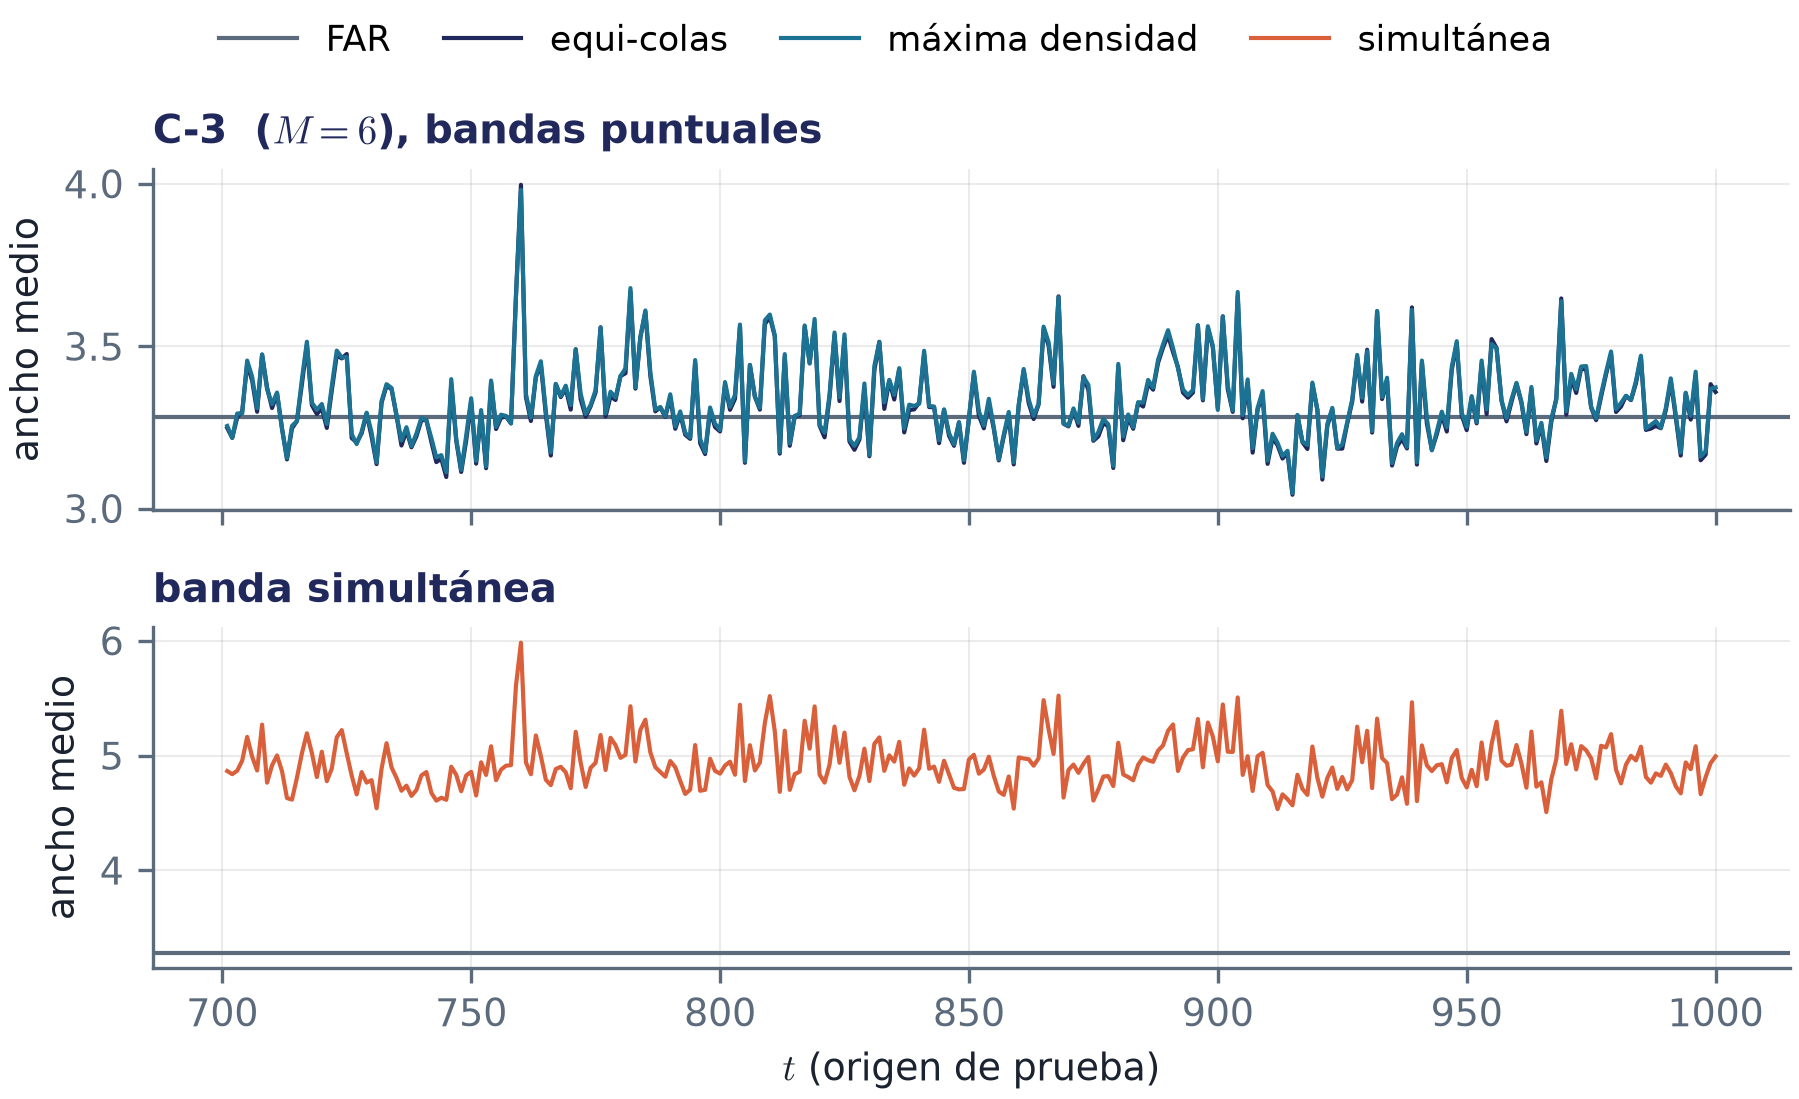
\includegraphics[width=\textwidth]{IMG/03_08/03_08_bloqueB_ancho_C3.png}
\caption{C-3. Ancho medio de la banda en cada origen de prueba ($M_{\mathrm{ref}}$) de las tres construcciones del PSBPM-FD y ancho fijo del FAR.}
\label{fig:res_bloqueB_ancho_C3}
\end{figure}

\subsection{Comportamientos predictivos}
\label{03_08_03_comportamientos}

Esta subsección y la siguiente se restringen a C-2. En C-1 y C-3 el modelo declara un solo comportamiento en el $99.7\%$ y el $100\%$ de los orígenes de prueba, como anticipa el diseño de la Sección~\ref{03_07_00_diseno_estudio_simulacion}. En C-2 se reporta primero cuántos comportamientos declara el modelo en el bloque de prueba completo para cada $M$ del barrido (Cuadro~\ref{tab:res_K}) y cómo se compara con los que tiene la ley verdadera. Luego se examinan de cerca diez orígenes consecutivos para mostrar qué es un comportamiento y qué ofrece frente a la esperanza (Figura~\ref{fig:res_ventana_detalle_C2}).

% Fuente: 102_K_por_M.csv de la 300 (bloque test).
\begin{table}[H]
\centering\small
\caption{Distribución de $K_t$ en el bloque de prueba de C-2 por $M$.}
\label{tab:res_K}
\begin{tabular}{c ccc}
\hline
$M$ & $K_t = 1$ & $K_t = 2$ & $K_t \ge 3$ \\
\hline
$1$ & 68.7\% & 31.3\% & 0.0\% \\
$2$ & 70.0\% & 15.7\% & 14.3\% \\
$3$ & 69.7\% & 15.7\% & 14.7\% \\
$4$ & 69.3\% & 16.7\% & 14.0\% \\
$5$ & 69.7\% & 16.7\% & 13.7\% \\
$6$ & 70.3\% & 16.3\% & 13.3\% \\
$7$ & 69.7\% & 16.7\% & 13.7\% \\
$8$ & 69.7\% & 16.7\% & 13.7\% \\
$9$ & 70.0\% & 16.7\% & 13.3\% \\
$10$ & 70.0\% & 16.7\% & 13.3\% \\
\hline
\end{tabular}
\end{table}

% Lectura K: los comportamientos aparecen donde la ley condicional reparte masa entre átomos separados.
En C-2 los comportamientos los producen los scores que cambian de régimen, ya que cerca del umbral los dos regímenes de un score son posibles a la vez y la mezcla pone un átomo en cada uno, de modo que el número de comportamientos lo fijan los scores con cambio de régimen y no cuántos scores entran al modelo. El Cuadro~\ref{tab:res_K} lo muestra en el barrido. Con $M = 1$ hay a lo más dos comportamientos, los dos regímenes del primer score. Con $M = 2$ aparece el tercero, porque el segundo score puede estar en un régimen distinto del primero y la mezcla separa esa combinación. Desde ahí la distribución no cambia con $M$, y los seis scores pasivos son autorregresivos sin regímenes, así que no abren comportamientos nuevos por más que se agreguen. Es lo que corresponde a la simulación, en que la dinámica de régimen vive en los primeros scores y el resto solo agrega variabilidad.\\

La ley verdadera tiene más de un modo en cerca de un $9\%$ de los orígenes de prueba, de modo que el modelo declara tres veces más de los que hay. La razón es que los pesos de la mezcla dependen de los rezagos a través de una transformación probit suave, que deja algo de masa en el átomo del régimen volátil también lejos del umbral, donde la probabilidad verdadera de ese régimen es casi nula. En los dos orígenes de la ventana de detalle en que la ley es bimodal, el modelo declara más de un comportamiento.\\

Las cifras anteriores resumen el bloque de prueba completo, pero no muestran qué es un comportamiento. Para eso se examinan de cerca $N_{\mathrm{det}} = 10$ orígenes consecutivos ($t = 807, \dots, 816$), el tramo del bloque de prueba con más cambios de régimen verdadero. 
% Figura: tres orígenes de la ventana de detalle de C-2. Fuente: comportamientos_psbp.npz y banda_funcional_psbp.npz del _04
% (curvas típicas, bandas condicionales, esperanza) y las curvas del generador.
\begin{figure}[H]
\centering
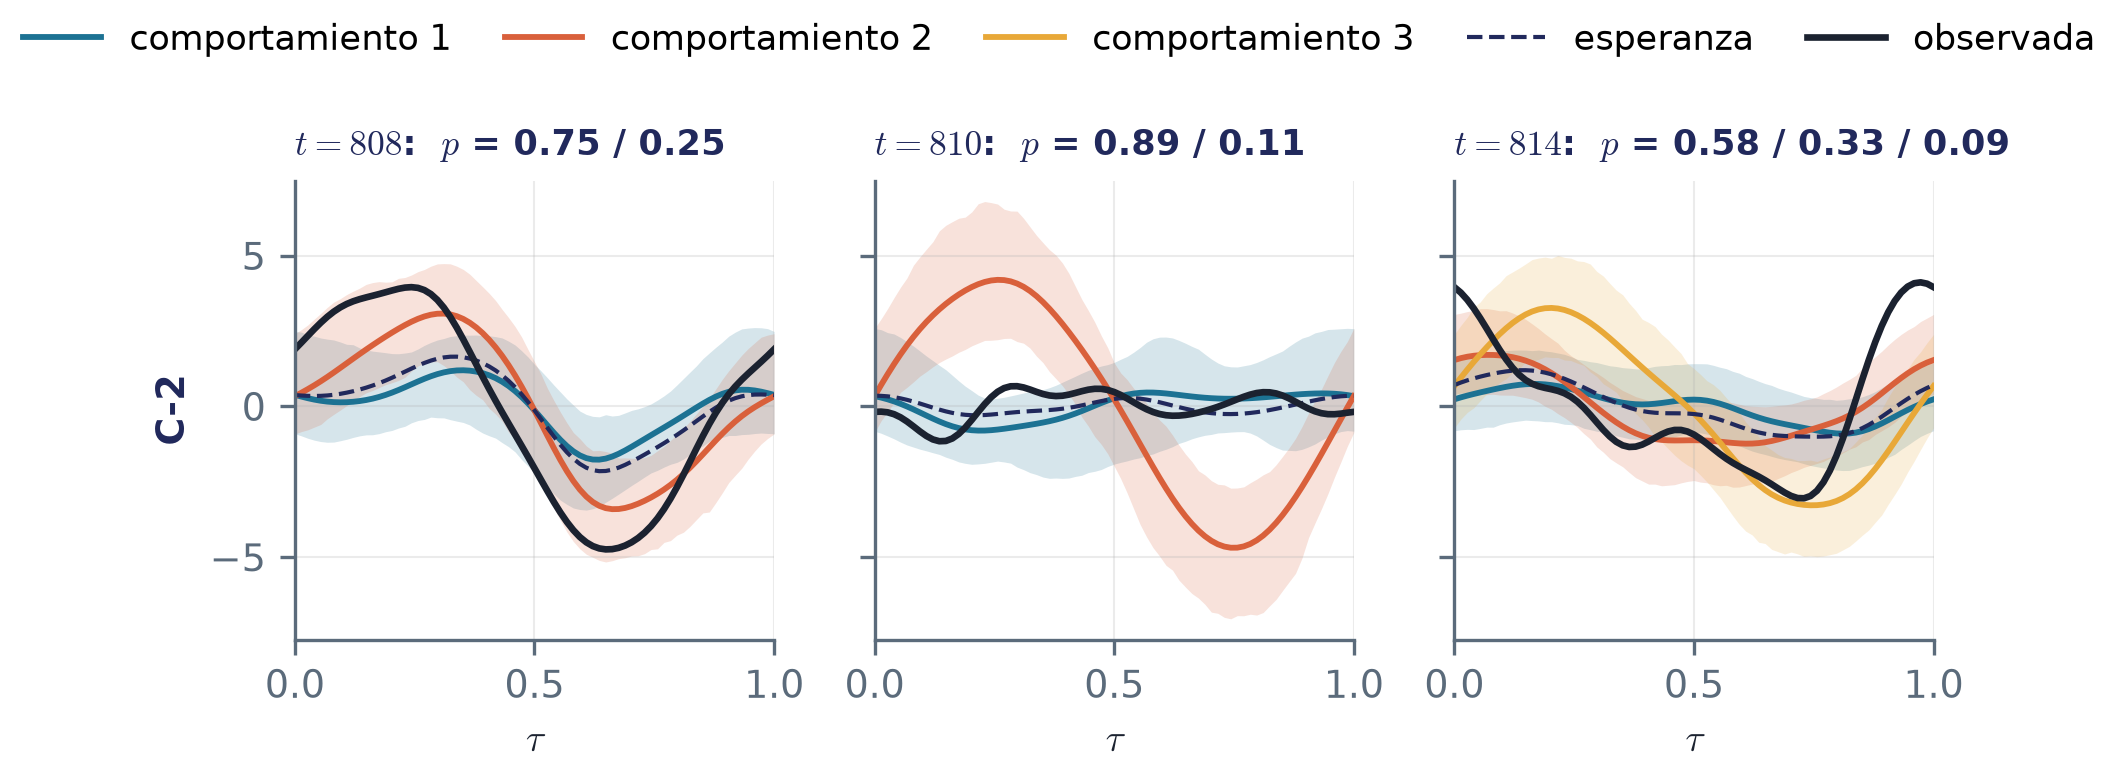
\includegraphics[width=\textwidth]{IMG/03_08/03_08_ventana_detalle_C2.png}
\caption{C-2. Tres orígenes de la ventana de detalle ($M_{\mathrm{ref}}$), con dos y tres comportamientos. Curva observada, esperanza y, por comportamiento, curva típica, banda condicional y probabilidad.}
\label{fig:res_ventana_detalle_C2}
\end{figure}

% Lectura detalle: para qué sirven los comportamientos y por qué el modelo acierta o falla en cada origen.
En los orígenes $807$ a $816$ el modelo declara más de un comportamiento en seis y la ley verdadera tiene más de un modo en dos, por la masa que los pesos probit dejan lejos del umbral, y aun así la curva observada cae en el comportamiento más probable en siete de los diez. En $t = 808$ el régimen cambió sin que el rezago lo anunciara y la curva observada sigue al comportamiento minoritario, cuya banda la cubre entera, mientras que la esperanza, que promedia los dos, queda en una curva que no ocurre. Es el caso en que una predictiva multimodal ofrece una opción que el promedio no tiene. En $t = 810$ acierta el más probable y el segundo es la masa que los pesos dejan en el régimen volátil. En $t = 814$ tres de los cuatro scores activos están en el régimen volátil, hay tres comportamientos y la curva observada se parece al segundo, pero sale de las bandas puntuales al final del dominio y solo la simultánea la contiene. Con qué frecuencia el comportamiento realizado es el más probable, y cuánto cuesta elegir mal, es lo que cuantifica la Sección~\ref{03_08_04_pronostico} sobre todo el bloque de prueba.

\subsection{Predicción por comportamiento}
\label{03_08_04_pronostico}

El Cuadro~\ref{tab:res_pronostico} resume, en $M_{\mathrm{ref}}$ de C-2, el error del pronóstico por comportamiento y de su cota \eqref{eq:mejor_comportamiento} frente a la esperanza y a las referencias, sobre todos los orígenes de prueba y sobre los que tienen más de un comportamiento. El Cuadro~\ref{tab:res_pronostico_por_M} y las Figuras~\ref{fig:res_pronostico_ventana_C2} y~\ref{fig:res_pronostico_ventana_rmse_C2} muestran lo mismo contra $M$ y sobre la ventana móvil, y el Cuadro~\ref{tab:res_acierto_p1} cuándo la elección por probabilidad acierta. Los dos cuadros promedian sobre los orígenes de prueba y no sobre las ventanas, porque el subconjunto con más de un comportamiento no es contiguo, y por eso sus cifras difieren en la tercera decimal de las de la Sección~\ref{03_08_01_error_puntual}.

% Fuente: 113_opciones_por_origen.csv del _06 (m10, test, opción "tipica"); MAE = media por origen, RMSE = raíz de la media de los cuadrados por origen. Coincide con 119_resumen_opciones_por_M.csv.
\begin{table}[H]
\centering\footnotesize
\caption{Pronóstico por comportamiento en el bloque de prueba de C-2 ($M_{\mathrm{ref}}$), sobre todos los orígenes y sobre los que tienen más de un comportamiento.}
\label{tab:res_pronostico}
\begin{tabular}{l cc cc}
\hline
 & \multicolumn{2}{c}{Todos los orígenes ($n = 300$)} & \multicolumn{2}{c}{$K_t \ge 2$ ($n = 90$)} \\
 & MAE & RMSE & MAE & RMSE \\
\hline
Pronóstico por comportamiento  & 0.607 & 0.793 & 0.619 & 0.847 \\
Cota (mejor comportamiento)    & 0.565 & 0.727 & 0.478 & 0.618 \\
Esperanza                      & 0.602 & 0.771 & 0.602 & 0.776 \\
FAR                            & 0.769 & 0.981 & 0.748 & 0.971 \\
Random Forest                  & 0.584 & 0.760 & 0.559 & 0.737 \\
\hline
\multicolumn{5}{l}{Fracción de orígenes} \\
El pronóstico gana al FAR            & \multicolumn{2}{c}{84\%} & \multicolumn{2}{c}{83\%} \\
El pronóstico gana al Random Forest  & \multicolumn{2}{c}{44\%} & \multicolumn{2}{c}{44\%} \\
La cota gana al FAR                  & \multicolumn{2}{c}{88\%} & \multicolumn{2}{c}{96\%} \\
La cota gana al Random Forest        & \multicolumn{2}{c}{49\%} & \multicolumn{2}{c}{61\%} \\
\hline
\end{tabular}
\end{table}

% Lectura pronóstico: elegir es una apuesta. Gana al FAR, no a la esperanza en promedio, y la cota dice cuánto hay en juego.
Elegir el comportamiento más probable es una apuesta, y por tanto, sobre todos los orígenes el pronóstico empata con la esperanza en MAE (0.607 frente a 0.602), porque en siete de cada diez coincide con ella, y es algo peor en RMSE. Las diferencias aparecen en los orígenes con más de un comportamiento, que muestra el Cuadro~\ref{tab:res_pronostico}. Frente al FAR gana con holgura, en el 83\% de ellos, porque cualquiera de los comportamientos es la curva de un régimen y el operador lineal no puede dar ninguna de ellas. Frente a la esperanza gana en el 59\% de esos orígenes y aun así pierde en promedio, porque cuando acierta el error baja, pero cuando el elegido no es el mejor el error sube más de lo que se ganó, porque la curva típica elegida queda lejos de la observada, mientras que la esperanza, al promediar, nunca queda tan lejos. Es el mismo motivo por el que el RMSE prefiere la esperanza. La cota dice cuánto hay en juego. En los orígenes con más de un comportamiento baja el error un quinto respecto de la esperanza y queda bajo el Random Forest, que es el mejor predictor puntual de C-2, de modo que entre las opciones que entrega el modelo casi siempre está la buena y lo que se pierde es por elegirla con la probabilidad, que acierta en el 78\% de esos orígenes. Sobre todos los orígenes, donde en siete de cada diez no hay nada que elegir, la ventaja de la cota es de un 6\% sobre la esperanza.

% Fuente: 113_opciones_por_origen.csv de cada M del _06 (test, opción "tipica"), medias por origen como en tab:res_pronostico.
\begin{table}[H]
\centering\footnotesize
\setlength{\tabcolsep}{3pt}
\caption{MAE y RMSE en el bloque de prueba de C-2 por $M$ del pronóstico por comportamiento, de la cota, de la esperanza, del FAR y del Random Forest.}
\label{tab:res_pronostico_por_M}
\begin{tabular}{c ccccc ccccc}
\hline
 & \multicolumn{5}{c}{MAE} & \multicolumn{5}{c}{RMSE} \\
$M$ & Pronóstico & Cota & Esperanza & FAR & RF & Pronóstico & Cota & Esperanza & FAR & RF \\
\hline
$1$ & 0.711 & 0.693 & 0.711 & 0.769 & 0.707 & 0.912 & 0.882 & 0.905 & 0.981 & 0.904 \\
$2$ & 0.670 & 0.636 & 0.666 & 0.769 & 0.651 & 0.862 & 0.811 & 0.849 & 0.981 & 0.838 \\
$3$ & 0.632 & 0.596 & 0.628 & 0.769 & 0.610 & 0.816 & 0.763 & 0.802 & 0.981 & 0.789 \\
$4$ & 0.612 & 0.570 & 0.605 & 0.769 & 0.584 & 0.799 & 0.733 & 0.777 & 0.981 & 0.762 \\
$5$ & 0.610 & 0.567 & 0.604 & 0.769 & 0.584 & 0.797 & 0.730 & 0.775 & 0.981 & 0.761 \\
$6$ & 0.608 & 0.568 & 0.603 & 0.769 & 0.585 & 0.795 & 0.730 & 0.773 & 0.981 & 0.761 \\
$7$ & 0.608 & 0.566 & 0.603 & 0.769 & 0.584 & 0.794 & 0.728 & 0.772 & 0.981 & 0.761 \\
$8$ & 0.608 & 0.565 & 0.603 & 0.769 & 0.584 & 0.793 & 0.727 & 0.772 & 0.981 & 0.761 \\
$9$ & 0.608 & 0.565 & 0.602 & 0.769 & 0.584 & 0.793 & 0.727 & 0.772 & 0.981 & 0.761 \\
$10$ & 0.607 & 0.565 & 0.602 & 0.769 & 0.584 & 0.793 & 0.727 & 0.771 & 0.981 & 0.760 \\
\hline
\end{tabular}
\end{table}

% Lectura trayectoria: la brecha entre cota y pronóstico está repartida en todo el test (contra M, 113 de cada M, no se tabula).
El Cuadro~\ref{tab:res_pronostico_por_M} muestra que la brecha entre la cota y el pronóstico se abre ya con $M = 1$ y deja de crecer en $M = 4$, como el resto del error puntual, porque los comportamientos los fijan los primeros scores. Las Figuras~\ref{fig:res_pronostico_ventana_C2} y~\ref{fig:res_pronostico_ventana_rmse_C2} muestran que la cota queda bajo la esperanza en todas las ventanas del bloque de prueba y bajo el pronóstico en el 87\% de ellas, porque los orígenes con más de un comportamiento están repartidos en él. La separación es mayor en el tramo de más cambios de régimen, donde el pronóstico queda por encima de la esperanza en todas las ventanas, porque ahí es donde más veces se elige mal.

% Figura: pronóstico y cota sobre la ventana móvil de prueba, w_ref, M_ref, contra FAR, RF y esperanza. Fuente: 115_ventana_modelos_w30.csv del _06.
\begin{figure}[H]
\centering
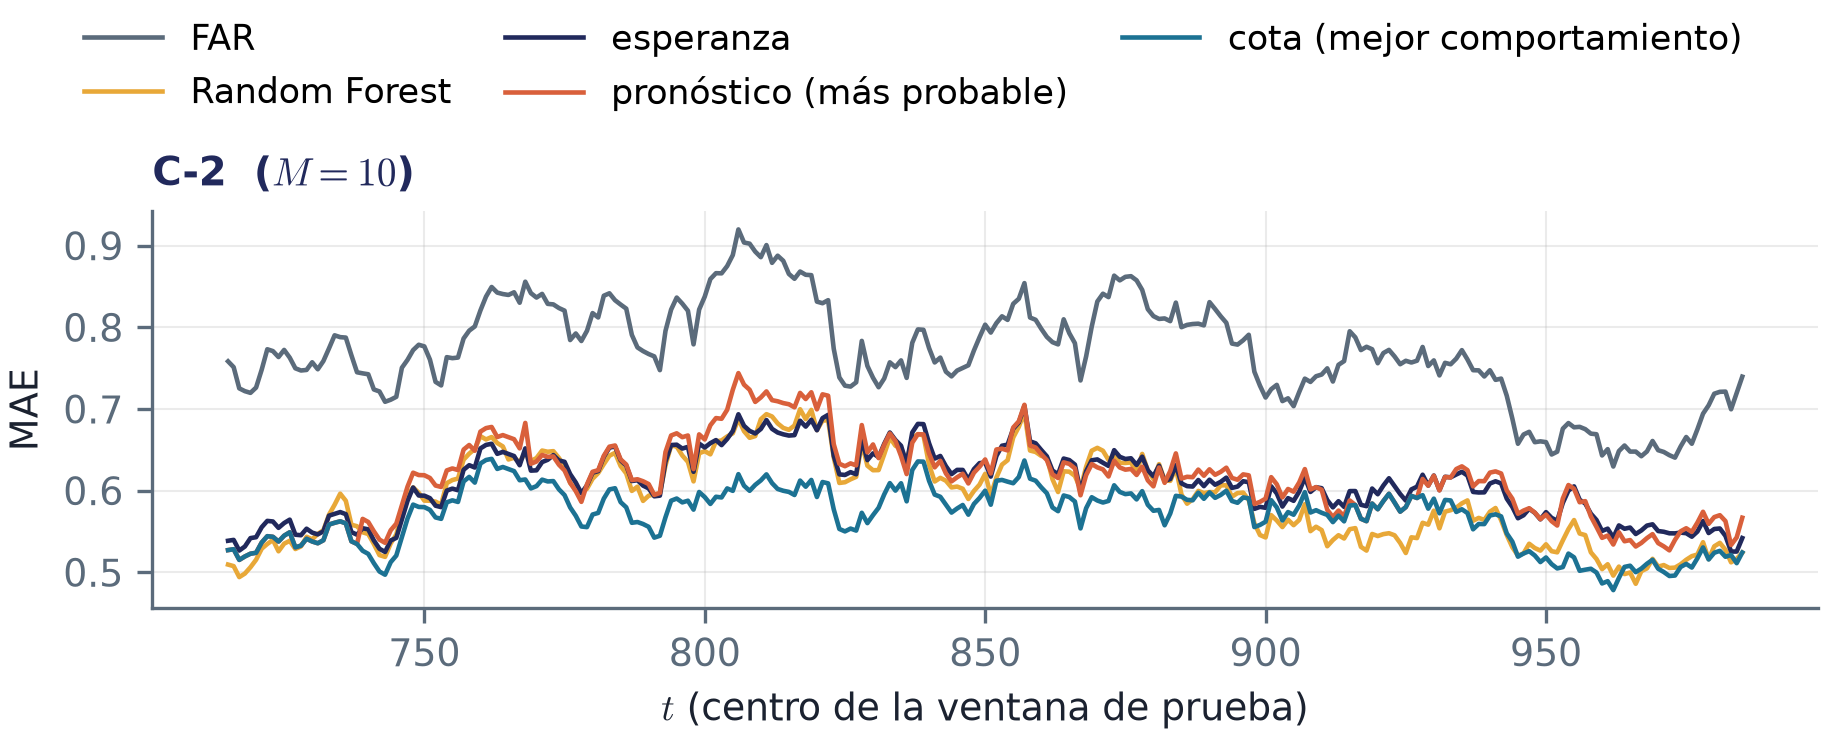
\includegraphics[width=\textwidth]{IMG/03_08/03_08_pronostico_ventana_w30_C2.png}
\caption{C-2. MAE del pronóstico por comportamiento y de la cota sobre la ventana móvil del bloque de prueba ($M_{\mathrm{ref}}$).}
\label{fig:res_pronostico_ventana_C2}
\end{figure}

\begin{figure}[H]
\centering
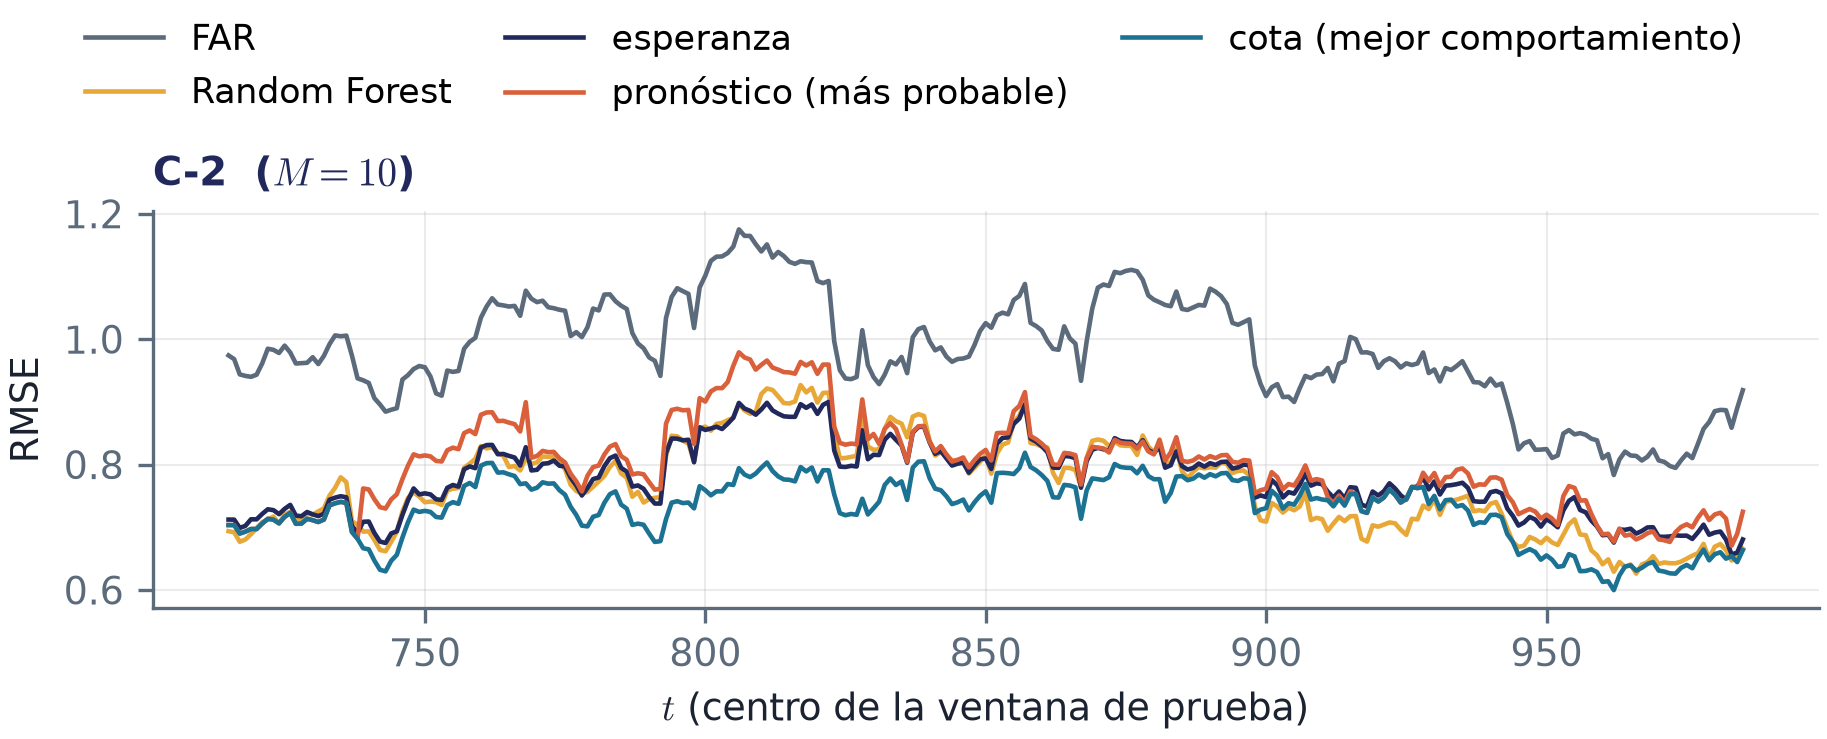
\includegraphics[width=\textwidth]{IMG/03_08/03_08_pronostico_ventana_rmse_w30_C2.png}
\caption{C-2. RMSE del pronóstico por comportamiento y de la cota sobre la ventana móvil del bloque de prueba ($M_{\mathrm{ref}}$).}
\label{fig:res_pronostico_ventana_rmse_C2}
\end{figure}

% Fuente: 119_acierto_por_p1.csv del _06 (test, K >= 2, M_ref). 83 de los 90 orígenes tienen p >= 0.5; los 7 restantes tienen K = 3 sin comportamiento dominante.
\begin{table}[H]
\centering\small
\caption{Acierto del pronóstico por comportamiento en C-2 ($K_t \ge 2$, $M_{\mathrm{ref}}$) por tramo de la probabilidad del comportamiento elegido. La última columna es el MAE que se pierde por elegir con la probabilidad en vez de la cota, en promedio sobre los orígenes del tramo. Los siete orígenes sin comportamiento dominante no se tabulan.}
\label{tab:res_acierto_p1}
\begin{tabular}{l c c c}
\hline
$p_{t,k^{*}}$ & Orígenes & Acierto & MAE pronóstico $-$ MAE cota \\
\hline
$[0.5, 0.6)$ & 5  & 20\%  & 0.61 \\
$[0.6, 0.7)$ & 11 & 36\%  & 0.28 \\
$[0.7, 0.8)$ & 31 & 87\%  & 0.11 \\
$[0.8, 0.9)$ & 28 & 93\%  & 0.06 \\
$[0.9, 1]$   & 8  & 100\% & 0.00 \\
\hline
\end{tabular}
\end{table}

% Lectura acierto: la probabilidad dice cuándo apostar. Entre 0.5 y 0.7 el acierto queda bajo una moneda y concentra cerca de la mitad de la pérdida.
La probabilidad del comportamiento elegido dice cuándo conviene apostar, como muestra el Cuadro~\ref{tab:res_acierto_p1}. Con una probabilidad alta el elegido es el mejor casi siempre y el pronóstico queda a un paso de la cota. Con masas entre un medio y $0.7$ el acierto cae por debajo de lo que daría una moneda, 5 de 16 orígenes en conjunto, y ahí se concentra cerca de la mitad de la pérdida. Con tan pocos orígenes no se puede separar si se debe al origen, con rezagos sobre el umbral donde el propio generador sortea el régimen con probabilidad cercana a un medio, o a una probabilidad optimista del modelo, coherente con la sobredetección de comportamientos de la Sección~\ref{03_08_03_comportamientos}. Tres de cada cuatro orígenes con más de un comportamiento tienen $p_{t,k^{*}} \ge 0.7$, y ahí el pronóstico queda cerca de la cota. Con una probabilidad alta se pronostica con el comportamiento, con una baja se reportan las opciones.

\section{Discusión}
\label{03_09}

En la predicción puntual, el PSBPM-FD supera al FAR en los tres escenarios, y lo hace de forma sostenida a lo largo del bloque de prueba y no solo en promedio. En C-2, donde la media condicional es no lineal, la esperanza reduce el MAE y el RMSE en torno a un $21\%$ y supera al FAR en todas las ventanas de prueba. En C-1 y C-3, donde la media condicional es lineal o casi lineal y la referencia está casi bien especificada, la reducción promedio es cercana al $2\%$, pero se repite en cerca de nueve de cada diez ventanas, y alguno de los tres predictores del PSBPM-FD es el mejor modelo en el $82\%$ y el $74\%$ de ellas. Una diferencia pequeña en el promedio corresponde, por tanto, a una ventaja consistente y no a unos pocos tramos favorables. Entre los predictores, la esperanza es la mejor bajo RMSE y la mediana puntual bajo MAE donde la predictiva es multimodal, como corresponde a la pérdida que cada una minimiza, y el átomo más probable es el más débil. En C-1 y C-2 el error deja de bajar en $M = 4$, la dimensión en que se observa toda la dinámica del generador; en C-3, donde los rezagos de todas las componentes entran a los pesos, el mínimo está en $M = 5$.\\

El Random Forest, con las mismas covariables, tiene un error mayor que el FAR en C-1 y queda por detrás del PSBPM-FD en más del $80\%$ de las ventanas de C-1 y C-3, pero es el mejor predictor puntual de C-2, en promedio y en dos de cada tres ventanas. Esto es coherente con la estructura de umbral del escenario, que sus cortes reproducen directamente, mientras que los pesos probit del PSBPM-FD cambian de forma suave. Aun así, la curva que lo supera suele estar entre las opciones de la predictiva del PSBPM-FD, ya que su cota tiene un MAE menor que el del Random Forest, sobre todo en los orígenes con más de un comportamiento ($0.478$ frente a $0.559$). La cota no es un predictor, de modo que la comparación no es justa en la práctica, pero indica que la desventaja del PSBPM-FD está en resumir una predictiva multimodal en una sola curva y no en la información que contiene.\\

Los intervalos son donde el modelo muestra su ventaja más clara. Las bandas puntuales del PSBPM-FD reducen el Winkler del FAR en un $20\%$ a $22\%$ en C-2 y en cerca de un $3\%$ en C-1 y C-3, y lo superan en entre el $73\%$ y el $100\%$ de las ventanas. En C-2 la reducción viene a la vez de una banda un $10\%$ más angosta y de una mayor cobertura; en C-1 y C-3, de una mejor calibración. La razón es que el ancho de la banda del PSBPM-FD se adapta al estado del proceso, angosta en los tramos tranquilos y ancha en los episodios de mayor varianza o en el régimen volátil, mientras que la banda del FAR hereda una varianza residual fija y tiene el mismo ancho en todos los orígenes. Esa adaptación es la que una ley de error rígida no puede dar, y es la razón por la que la ventaja en los intervalos aparece incluso donde la media condicional es lineal. La región de máxima densidad solo se separa de la equi-colas en C-2, donde la predictiva tiene valles, y ahí es la mejor banda en nueve de cada diez ventanas. La banda simultánea pierde el Winkler por ser más ancha, pero es la única que cubre la curva completa con una frecuencia cercana a la nominal.\\

Los comportamientos predictivos responden a los cambios de régimen. En C-2 la predictiva tiene más de un comportamiento en el $30\%$ de los orígenes de prueba, y su número lo fijan los scores con cambio de régimen y no la dimensión $M$. En C-1 y C-3 la predictiva tiene un solo comportamiento en casi todos los orígenes. En C-3 la multimodalidad del generador queda en la ley conjunta de los scores y no llega a la curva, de modo que los comportamientos detectan los modos de la curva siguiente y no los de cualquier mecanismo latente. El pronóstico con el comportamiento más probable empata con la esperanza en MAE sobre todo el bloque de prueba y la supera en el $59\%$ de los orígenes con más de un comportamiento, pero pierde en promedio porque las elecciones equivocadas pesan más que las acertadas. Su cota reduce el error de la esperanza en un quinto, de modo que la opción correcta suele estar entre las que entrega el modelo y la pérdida se produce al elegirla. La probabilidad del comportamiento elegido indica cuándo conviene hacerlo.\\

Los comportamientos admiten además una lectura como agrupamiento. Cuando el cambio de régimen lo gobierna una variable latente que los rezagos revelan solo en parte, los comportamientos funcionan como un agrupamiento de la curva siguiente por estado latente, con la probabilidad de cada uno. En C-2 el agrupamiento sigue al régimen del generador; el capítulo siguiente examina el caso de un estado latente en datos reales.\\

La principal limitación de los comportamientos es la sobredetección. El modelo declara más de un comportamiento en el $30\%$ de los orígenes de prueba de C-2, mientras que la ley verdadera es multimodal solo en cerca de un $9\%$, porque la transición probit suave deja masa en el régimen volátil lejos del umbral. En la misma línea, cuando la probabilidad del comportamiento elegido está entre $0.5$ y $0.7$, el acierto es de 5 en 16 orígenes, por debajo de lo que esa probabilidad indica; con tan pocos orígenes no puede separarse si se debe a rezagos sobre el umbral o a una probabilidad optimista del modelo.\\

En la práctica, el resumen que conviene reportar depende de la forma de la predictiva en cada origen, que los comportamientos permiten leer. Cuando la predictiva tiene un solo comportamiento, la esperanza resume bien la curva siguiente; cuando tiene más de uno, conviene acompañarla de la mediana puntual o del pronóstico por comportamiento, según la probabilidad de cada opción. Entre los intervalos, la banda equi-colas es la construcción de referencia, la simultánea es la opción conservadora cuando interesa cubrir la curva completa, a costa de un ancho mayor, y la de máxima densidad es la más ajustada cuando la predictiva tiene valles. En cuanto a la dimensión, con rezagos propios agregar componentes no empeora el error puntual, que se estabiliza una vez cubiertos los scores con dinámica, mientras que con los rezagos de todas las componentes cada score adicional agranda el conjunto de covariables de los pesos de la mezcla y uno sin dinámica puede empeorarlo, como ocurre en C-3 con $M = 6$. La factorización hace además que los $M$ muestreadores sean independientes y puedan ejecutarse en paralelo, y con rezagos propios basta entrenar el mayor $M$ del barrido y reutilizar sus trazas para los menores.











\chapter{Aplicación a Datos Reales}
\label{04_00_00_aplicacion}


Este capítulo aplica el PSBPM-FD a una serie observada de curvas diarias, el volumen horario de vehículos en una autopista urbana, con el propósito aplicado de pronosticar con un día de anticipación el perfil completo de tráfico del día siguiente y cuantificar su incertidumbre. Un pronóstico de este tipo no se agota en una curva media, porque la pregunta operativa no es solo cuántos vehículos circularán en promedio sino si el día siguiente tendrá las horas punta de un día laborable o el perfil plano de un fin de semana o un feriado, y con qué probabilidad.\\

La serie se eligió porque reúne, en datos reales, el rasgo que en el estudio de simulación favorecía al modelo propuesto (escenario C-2, Sección~\ref{03_07_02_escenarios}), ya que la ley de la curva siguiente depende de un estado del proceso, el tipo de día, que la curva anterior solo revela en parte. Cuando ese estado no se observa, la distribución predictiva debería repartir su masa entre perfiles distintos, y cuando se observa, debería concentrarla en uno. Para estudiar ese efecto se ajustan dos especificaciones que difieren únicamente en la información de la que dependen los pesos de la mezcla, la primera usa la curva del día anterior y la segunda agrega la del mismo día de la semana anterior. La comparación entre ambas muestra cómo la mezcla pasa de una predictiva con varios comportamientos a una unimodal a medida que las covariables contienen la información relevante sobre el estado. Como el tipo de día no entra a ningún método, la serie permite además comprobar que, cuando el régimen lo gobierna un estado latente que los rezagos revelan solo en parte, los comportamientos de la predictiva agrupan la curva siguiente según ese estado.\\

El capítulo describe primero los datos y la evidencia descriptiva que motiva el modelo, luego el diseño de la comparación y, por último, los resultados en el mismo orden que el estudio de simulación. Los gráficos complementarios de esta aplicación se reúnen en el Anexo~\ref{aneC_00_00_trafico} y los resultados de otras cinco series reales, en las que la predictiva resultó unimodal, en el Anexo~\ref{aneD_00_00_otras_series}.

\section{Datos}
\label{04_01_00_datos}

Los datos provienen del conjunto \textbf{Metro Interstate Traffic Volume} del UCI Machine Learning Repository \citep{04_01_hogue2019metro}, que registra el volumen horario de vehículos en la estación ATR 301 del Departamento de Transporte de Minnesota, en la autopista I-94 en dirección oeste, entre Minneapolis y Saint Paul.\\

Se usa la ventana del 1 de julio de 2015 al 30 de septiembre de 2018, que da $T = 1188$ días. Cada día es una curva observada en $G = 24$ horas, con el volumen en miles de vehículos por hora.\\

El registro tiene huecos que suman un $7\%$ de las horas de la ventana, y cada día se representa en una base B-spline cúbica de $J = 10$ funciones según la cantidad de horas observadas:
\begin{itemize}
    \item Los días completos se ajustan directamente a sus 24 horas.
    \item Los 301 días incompletos se ajustan solo a las horas observadas, con una penalización débil hacia el perfil medio del bloque de entrenamiento.
    \item Los días sin dato, del 24 al 26 de octubre de 2015, y los que tienen más de doce horas ausentes reciben coeficientes interpolados linealmente en el tiempo.
\end{itemize}
Sobre esa representación se estima la FPCA con el bloque de entrenamiento y se retienen $M = 10$ componentes, que reproducen la representación completa.\\

La serie se parte en orden cronológico en un bloque de entrenamiento de 831 días (1 de julio de 2015 al 8 de octubre de 2017) y uno de prueba de 357 días (9 de octubre de 2017 al 30 de septiembre de 2018).

\subsection{Análisis descriptivo}
\label{04_01_01_descriptivo}

La Figura~\ref{fig:apl_perfiles} muestra las curvas del bloque de entrenamiento separadas por tipo de día, con la mediana puntual y la banda entre los cuantiles $10\%$ y $90\%$. Los días laborables tienen dos horas punta, hacia las siete de la mañana y las cuatro de la tarde, con medianas por sobre seis mil vehículos por hora, mientras que los sábados, domingos y feriados tienen un solo máximo amplio al mediodía, más bajo y con un ascenso más tardío en la mañana. El nivel medio del día pasa de $3.61$ mil vehículos por hora en los laborables a $2.85$ en los sábados y $2.50$ en los domingos y feriados. La dispersión dentro de cada tipo es pequeña frente a la distancia entre tipos, de modo que la distribución marginal de la curva es, en buena medida, una mezcla de pocos perfiles bien separados.

\begin{figure}[H]
\centering
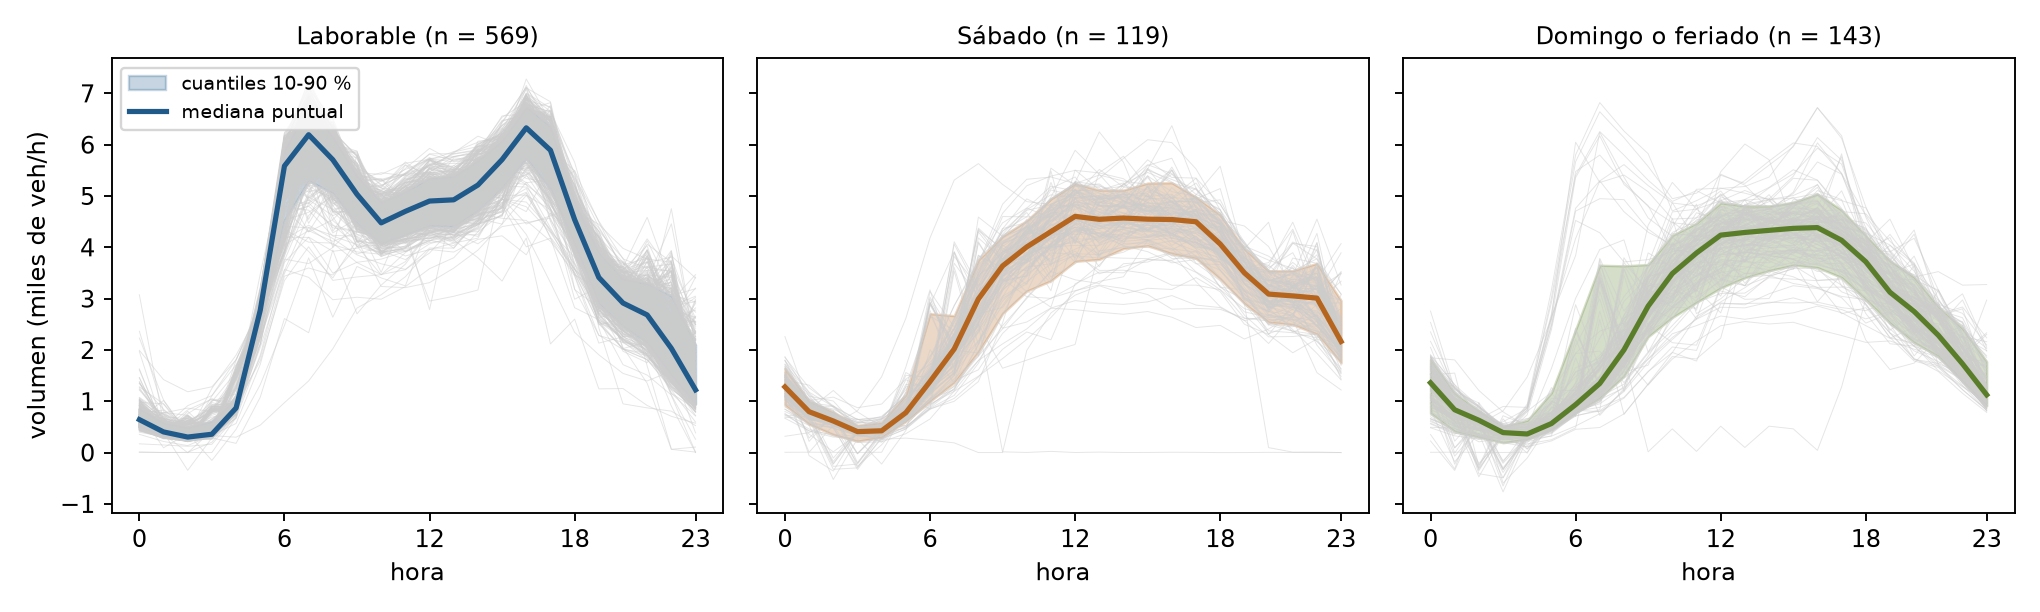
\includegraphics[width=\textwidth,height=0.4\textheight,keepaspectratio]{IMG/04_01/04_perfiles_tipo_dia.png}
\caption{Curvas diarias del bloque de entrenamiento por tipo de día, con la mediana puntual y la banda entre los cuantiles $10\%$ y $90\%$.}
\label{fig:apl_perfiles}
\end{figure}

La Figura~\ref{fig:apl_nivel} muestra el nivel medio de cada día a lo largo de la ventana. Los días laborables forman una franja separada de la de los fines de semana, en la que sábados y domingos quedan próximos entre sí, y ninguna de las franjas tiene tendencia marcada, salvo un nivel laborable algo más bajo en el segundo semestre de 2016. 

\begin{figure}[H]
\centering
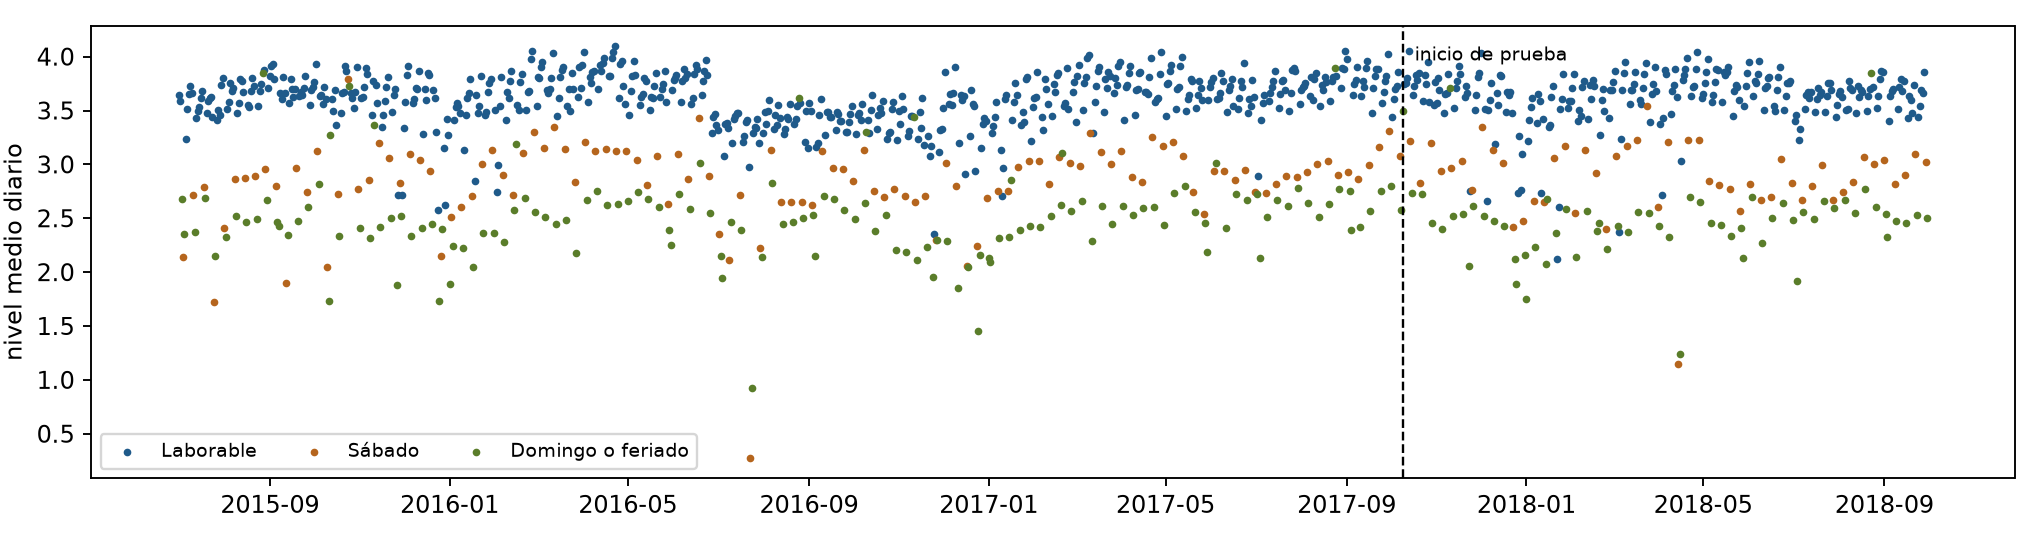
\includegraphics[width=\textwidth,height=0.3\textheight,keepaspectratio]{IMG/04_01/04_nivel_diario.png}
\caption{Nivel medio diario del volumen de tráfico por tipo de día. La línea discontinua marca el inicio del bloque de prueba.}
\label{fig:apl_nivel}
\end{figure}

La Figura~\ref{fig:apl_dependencia} relaciona el primer score, que distingue el perfil laborable del de fin de semana, con su valor un día y una semana antes. Frente al rezago de un día, los puntos forman cuatro nubes, una por cada transición, de laborable a laborable, de viernes a sábado, de sábado a domingo y de domingo a lunes. Un mismo valor del rezago lleva así a destinos distintos, porque tras un día laborable el siguiente puede ser otro laborable o un sábado, y el tercer panel lo muestra de forma directa, pues, condicionado a un rezago en el rango típico de un día laborable, la distribución del score siguiente es bimodal, con un $24\%$ de la masa en el perfil de fin de semana. Una relación lineal con el rezago de un día promedia esos dos destinos en un valor intermedio que no corresponde a ningún día, y por eso explica solo el $16\%$ de la varianza del primer score (correlación $0.40$). Frente al rezago de una semana, en cambio, cada día se compara con el mismo día de la semana anterior, que casi siempre es del mismo tipo, de modo que los puntos se alinean sobre la diagonal y la correlación sube a $0.83$.

\begin{figure}[H]
\centering
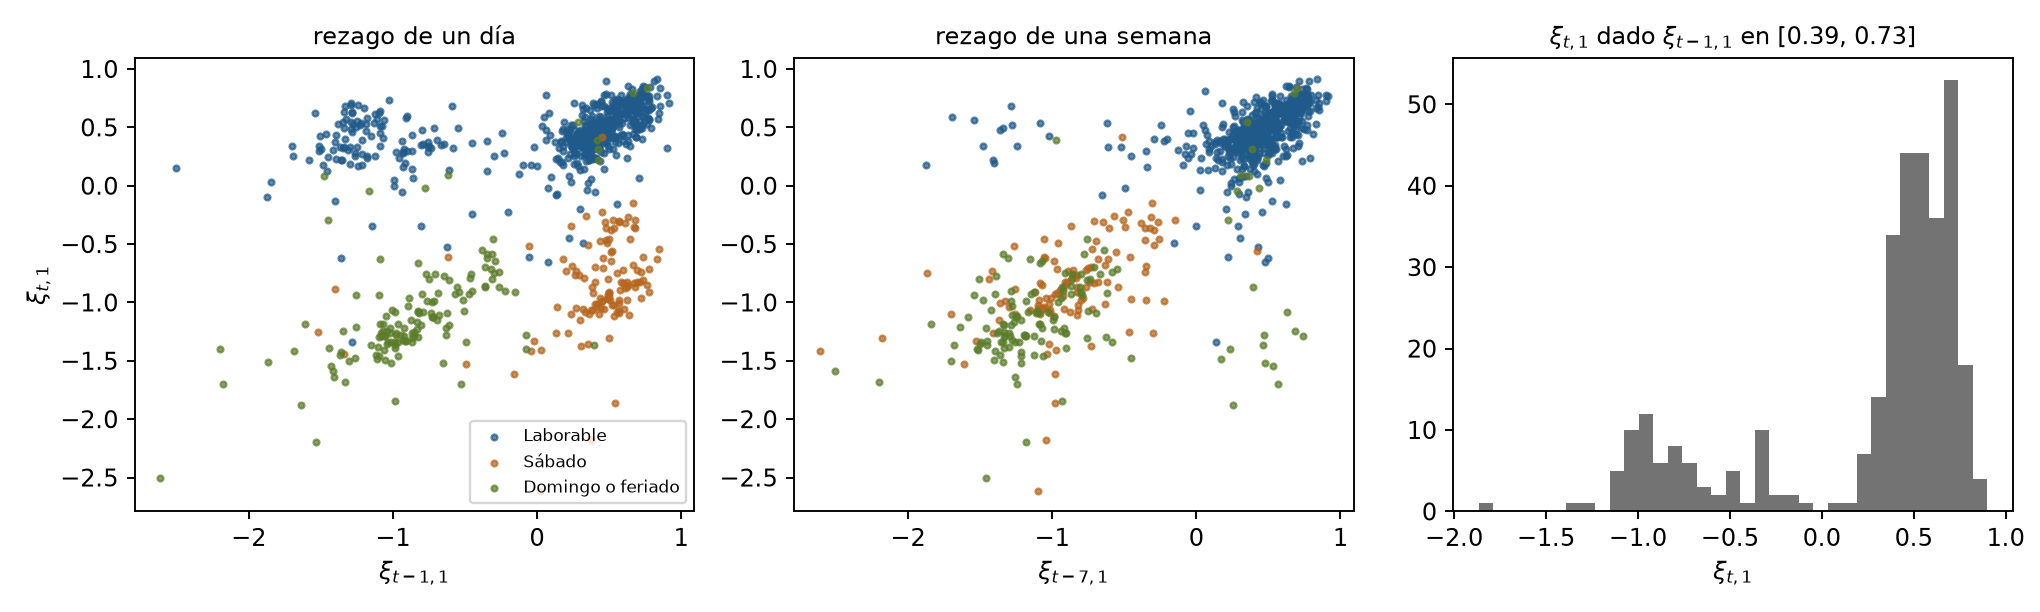
\includegraphics[width=\textwidth,height=0.4\textheight,keepaspectratio]{IMG/04_01/04_dependencia_score1.png}
\caption{Primer score frente a su rezago de un día (izquierda) y de una semana (centro), por tipo de día predicho, y distribución del primer score condicionada a un rezago de un día en el rango típico de los días laborables (derecha). Bloque de entrenamiento.}
\label{fig:apl_dependencia}
\end{figure}

Por tanto, la evidencia descriptiva justifica el uso del modelo propuesto en dos sentidos. Primero, con la información del día anterior la ley de la curva siguiente es una mezcla de perfiles, que un predictor lineal resume en un promedio que no corresponde a ningún día real, mientras que una mezcla con pesos dependientes de las covariables puede asignar un átomo a cada perfil y una probabilidad a cada uno. Segundo, el estado que decide el perfil, el tipo de día, está contenido en buena parte en el rezago semanal, de modo que agregarlo a las covariables de los pesos de la mezcla debería concentrar la masa en el perfil correcto.

\section{Diseño}
\label{04_02_00_diseno}

El diseño sigue al del estudio de simulación (Sección~\ref{03_07_00_diseno_estudio_simulacion}), con las diferencias que impone trabajar con una sola serie observada. Todo lo que se estima con datos, la base, la FPCA, los hiperparámetros del modelo propuesto y los modelos de referencia, se estima solo con el bloque de entrenamiento. Sobre el bloque de prueba se calculan predicciones a un paso con los rezagos observados, sin reestimar ningún modelo, y el calendario no entra a ningún método, se usa solo para leer los resultados.\\

Se ajustan dos especificaciones del PSBPM-FD que difieren en las covariables. En la primera, el score $m$ del día $t$ depende de los diez scores del día $t-1$; en la segunda, de los diez scores de los días $t-1$ y $t-7$, veinte covariables en total. En ambas, cada score tiene su propia mezcla y los pesos de la mezcla dependen de todas las covariables, de modo que la información del rezago semanal puede cambiar los pesos de los átomos sin cambiar su forma. El modelo se ajusta con los hiperparámetros de \citet{03_02_chung2009nonparametric} expresados en la escala de cada score, con $a_\nu = 2$, que a diferencia del valor $0.5$ del estudio de simulación garantiza que la varianza predictiva exista, y con un truncamiento de 30 átomos. El muestreador se ejecuta con una cadena de 2500 iteraciones, de las que se descartan las primeras 1000 como calentamiento; con una sola cadena no se calcula $\widehat{R}$, y los diagnósticos se hacen sobre cantidades invariantes a la permutación de las etiquetas de los átomos.\\

Las referencias son las del estudio de simulación. El FAR se ajusta sobre los coeficientes de la base con orden igual al mayor rezago de cada especificación, uno en la primera y siete en la segunda, y su intervalo es la banda gaussiana de su residuo. El Random Forest ajusta un bosque por score con las mismas covariables que el PSBPM-FD y elige el conjunto de rezagos con el bloque de entrenamiento. Solo el FAR y el PSBPM-FD entregan intervalos.\\

Los resultados se presentan como en la Sección~\ref{03_08_00_resultados}. Las métricas de la Sección~\ref{02_02_03_criterios_evaluacion} se calculan sobre la ventana móvil de ancho $w = 30$ sobre el bloque de prueba, contra la curva ajustada por la representación (Sección~\ref{03_05_00_reconstruccion_funcional}), y los cuadros reportan su promedio sobre las ventanas y la fracción de ventanas que gana cada modelo. Del PSBPM-FD se reportan los tres predictores puntuales de la Sección~\ref{03_05_04_predictores_puntuales}, con la regla de consistencia según la cual el MAE corresponde a la mediana puntual y el RMSE a la esperanza, y las tres construcciones de intervalo de la Sección~\ref{03_05_05_intervalos_predictivos}. Los comportamientos predictivos (Sección~\ref{03_06_00_comportamientos}) se resumen por la distribución de $K_t$ en el bloque de prueba y se contrastan con el calendario, que aquí reemplaza al régimen verdadero de la simulación. Para mostrar qué es un comportamiento se analiza una ventana de detalle de diez días consecutivos de prueba, elegida por tener la mayor cantidad de días no laborables, del 23 de diciembre de 2017 al 1 de enero de 2018, con dos fines de semana, Navidad y Año Nuevo. Se evalúa además el pronóstico por comportamiento de la Sección~\ref{03_06_03_descripcion} y su cota \eqref{eq:mejor_comportamiento}, y, por último, se analizan las probabilidades posteriores de inclusión de los rezagos en la mezcla de cada score. La configuración completa de la aplicación está en el Anexo~\ref{aneC_00_01_configuracion}.

Los resultados siguen el orden del estudio de simulación, es decir, error puntual, intervalos de predicción, comportamientos predictivos y el pronóstico que se construye con ellos, y se agrega al final la selección de variables. En cada apartado se contrastan las dos especificaciones, porque la diferencia entre ellas es la que muestra el efecto de la información sobre los pesos de la mezcla.

\subsection{Error puntual}
\label{04_03_01_error_puntual}

Los Cuadros~\ref{tab:apl_bloqueA} y~\ref{tab:apl_bloqueA_ganancia} resumen el MAE y el RMSE promedio sobre las ventanas de prueba de los tres predictores del PSBPM-FD y de las dos referencias, y el cambio relativo respecto del FAR.

% Fuente: 98_resumen_bloqueA_min_max_prom.csv del _05 (test, promedio sobre ventanas).
\begin{table}[H]
\centering\small
\setlength{\tabcolsep}{3.5pt}
\caption{MAE y RMSE en el bloque de prueba del tráfico ($M = 10$, $w = 30$). En negrita el menor de cada fila.}
\label{tab:apl_bloqueA}
\begin{tabular}{l ccccc ccccc}
\hline
Rezagos & \multicolumn{5}{c}{MAE} & \multicolumn{5}{c}{RMSE} \\
 & Esp. & Med. & Modal & RF & FAR & Esp. & Med. & Modal & RF & FAR \\
\hline
$\{1\}$ & 0.413 & 0.376 & 0.397 & \textbf{0.361} & 0.398 & 0.646 & 0.658 & 0.729 & \textbf{0.562} & 0.621 \\
$\{1,7\}$ & 0.315 & \textbf{0.302} & 0.317 & 0.314 & 0.314 & 0.522 & 0.528 & 0.556 & 0.499 & \textbf{0.495} \\
\hline
\end{tabular}
\end{table}

\begin{table}[H]
\centering\small
\setlength{\tabcolsep}{3.5pt}
\caption{Cambio relativo del MAE y del RMSE respecto del FAR por predictor. Negativo es mejor que el FAR.}
\label{tab:apl_bloqueA_ganancia}
\begin{tabular}{l cc cc cc cc}
\hline
Rezagos & \multicolumn{2}{c}{Esperanza} & \multicolumn{2}{c}{Mediana} & \multicolumn{2}{c}{Modal} & \multicolumn{2}{c}{RF} \\
 & MAE & RMSE & MAE & RMSE & MAE & RMSE & MAE & RMSE \\
\hline
$\{1\}$ & $+3.8\%$ & $+4.1\%$ & $-5.4\%$ & $+5.9\%$ & $-0.1\%$ & $+17.4\%$ & $-9.3\%$ & $-9.6\%$ \\
$\{1,7\}$ & $+0.1\%$ & $+5.6\%$ & $-3.7\%$ & $+6.6\%$ & $+1.0\%$ & $+12.3\%$ & $0.0\%$ & $+0.8\%$ \\
\hline
\end{tabular}
\end{table}
Al agregar el rezago semanal, el MAE de todos los modelos baja entre un $13\%$ y un $24\%$, y el FAR con ambos rezagos ($0.314$) queda por debajo de cualquier modelo con solo el rezago de un día, incluido el Random Forest ($0.361$). Además, la comparación entre los predictores del PSBPM-FD reproduce lo que anticipa la forma de la predictiva. Con el rezago de un día, donde la predictiva tiene dos comportamientos en la mayoría de los orígenes (Sección~\ref{04_03_03_comportamientos}), la esperanza queda entre el perfil laborable y el de fin de semana, en una curva que no ocurre, y pierde frente al FAR en las dos métricas. La mediana puntual se inclina hacia el comportamiento dominante y baja el MAE del FAR en un $5.4\%$, pero cuando el comportamiento dominante no es el que ocurre su error es grande y su RMSE sube, que es el reparto que corresponde a lo que mide cada métrica. El átomo más probable es el peor en RMSE en las dos especificaciones. Con ambos rezagos, la mediana sigue siendo la mejor en MAE ($-3.7\%$) y la esperanza, el FAR y el Random Forest quedan a menos de un $1\%$ entre sí, mientras que en RMSE el FAR es el mejor.\\

El Random Forest es el mejor modelo con el rezago de un día, por un margen de un $9\%$ sobre el FAR en las dos métricas, y su ventaja desaparece con el rezago semanal. Con una sola covariable diaria, la partición por umbrales del bosque separa los destinos posibles de un día laborable mejor que un promedio, y cuando el rezago semanal resuelve el tipo de día la parte lineal de la dinámica basta y las diferencias entre métodos desaparecen.

% Fuente: 72_ventana_modelos_w30.csv del _05 (test, w = 30, sin el medoide).
\begin{table}[H]
\centering\small
\setlength{\tabcolsep}{3.5pt}
\caption{Ventanas de prueba ganadas por modelo, por MAE y por RMSE.}
\label{tab:apl_bloqueA_ventanas}
\begin{tabular}{l ccccc ccccc}
\hline
Rezagos & \multicolumn{5}{c}{MAE} & \multicolumn{5}{c}{RMSE} \\
 & FAR & RF & Esp. & Med. & Modal & FAR & RF & Esp. & Med. & Modal \\
\hline
$\{1\}$ & 7\% & 54\% & 0\% & 25\% & 14\% & 11\% & 78\% & 0\% & 9\% & 1\% \\
$\{1,7\}$ & 18\% & 19\% & 1\% & 59\% & 3\% & 43\% & 37\% & 1\% & 19\% & 0\% \\
\hline
\end{tabular}
\end{table}

\begin{table}[H]
\centering\small
\setlength{\tabcolsep}{3.5pt}
\caption{Fracción de ventanas en que el predictor consistente del PSBPM-FD supera a cada referencia (mediana en MAE, esperanza en RMSE).}
\label{tab:apl_bloqueA_gana}
\begin{tabular}{l cc cc}
\hline
Rezagos & \multicolumn{2}{c}{MAE (mediana)} & \multicolumn{2}{c}{RMSE (esperanza)} \\
 & vs FAR & vs RF & vs FAR & vs RF \\
\hline
$\{1\}$ & 70\% & 42\% & 27\% & 1\% \\
$\{1,7\}$ & 80\% & 73\% & 21\% & 30\% \\
\hline
\end{tabular}
\end{table}

Los Cuadros~\ref{tab:apl_bloqueA_ventanas} y~\ref{tab:apl_bloqueA_gana} muestran que los promedios se sostienen a lo largo del bloque de prueba. Bajo MAE, la mediana puntual supera al FAR en siete de cada diez ventanas con el rezago de un día y en ocho de cada diez con ambos rezagos, y con ambos rezagos es el mejor modelo en el $59\%$ de las ventanas y supera al Random Forest en el $73\%$. Bajo RMSE la ventaja es de las referencias, ya que la esperanza supera al FAR en menos de un tercio de las ventanas en las dos especificaciones, y con el rezago de un día el Random Forest gana el $78\%$ de ellas.

% Fuente: 72_ventana_modelos_w30.csv de 101 y 102 (test, sin el medoide); figura en docs/IMG/04_03.
\begin{figure}[H]
\centering
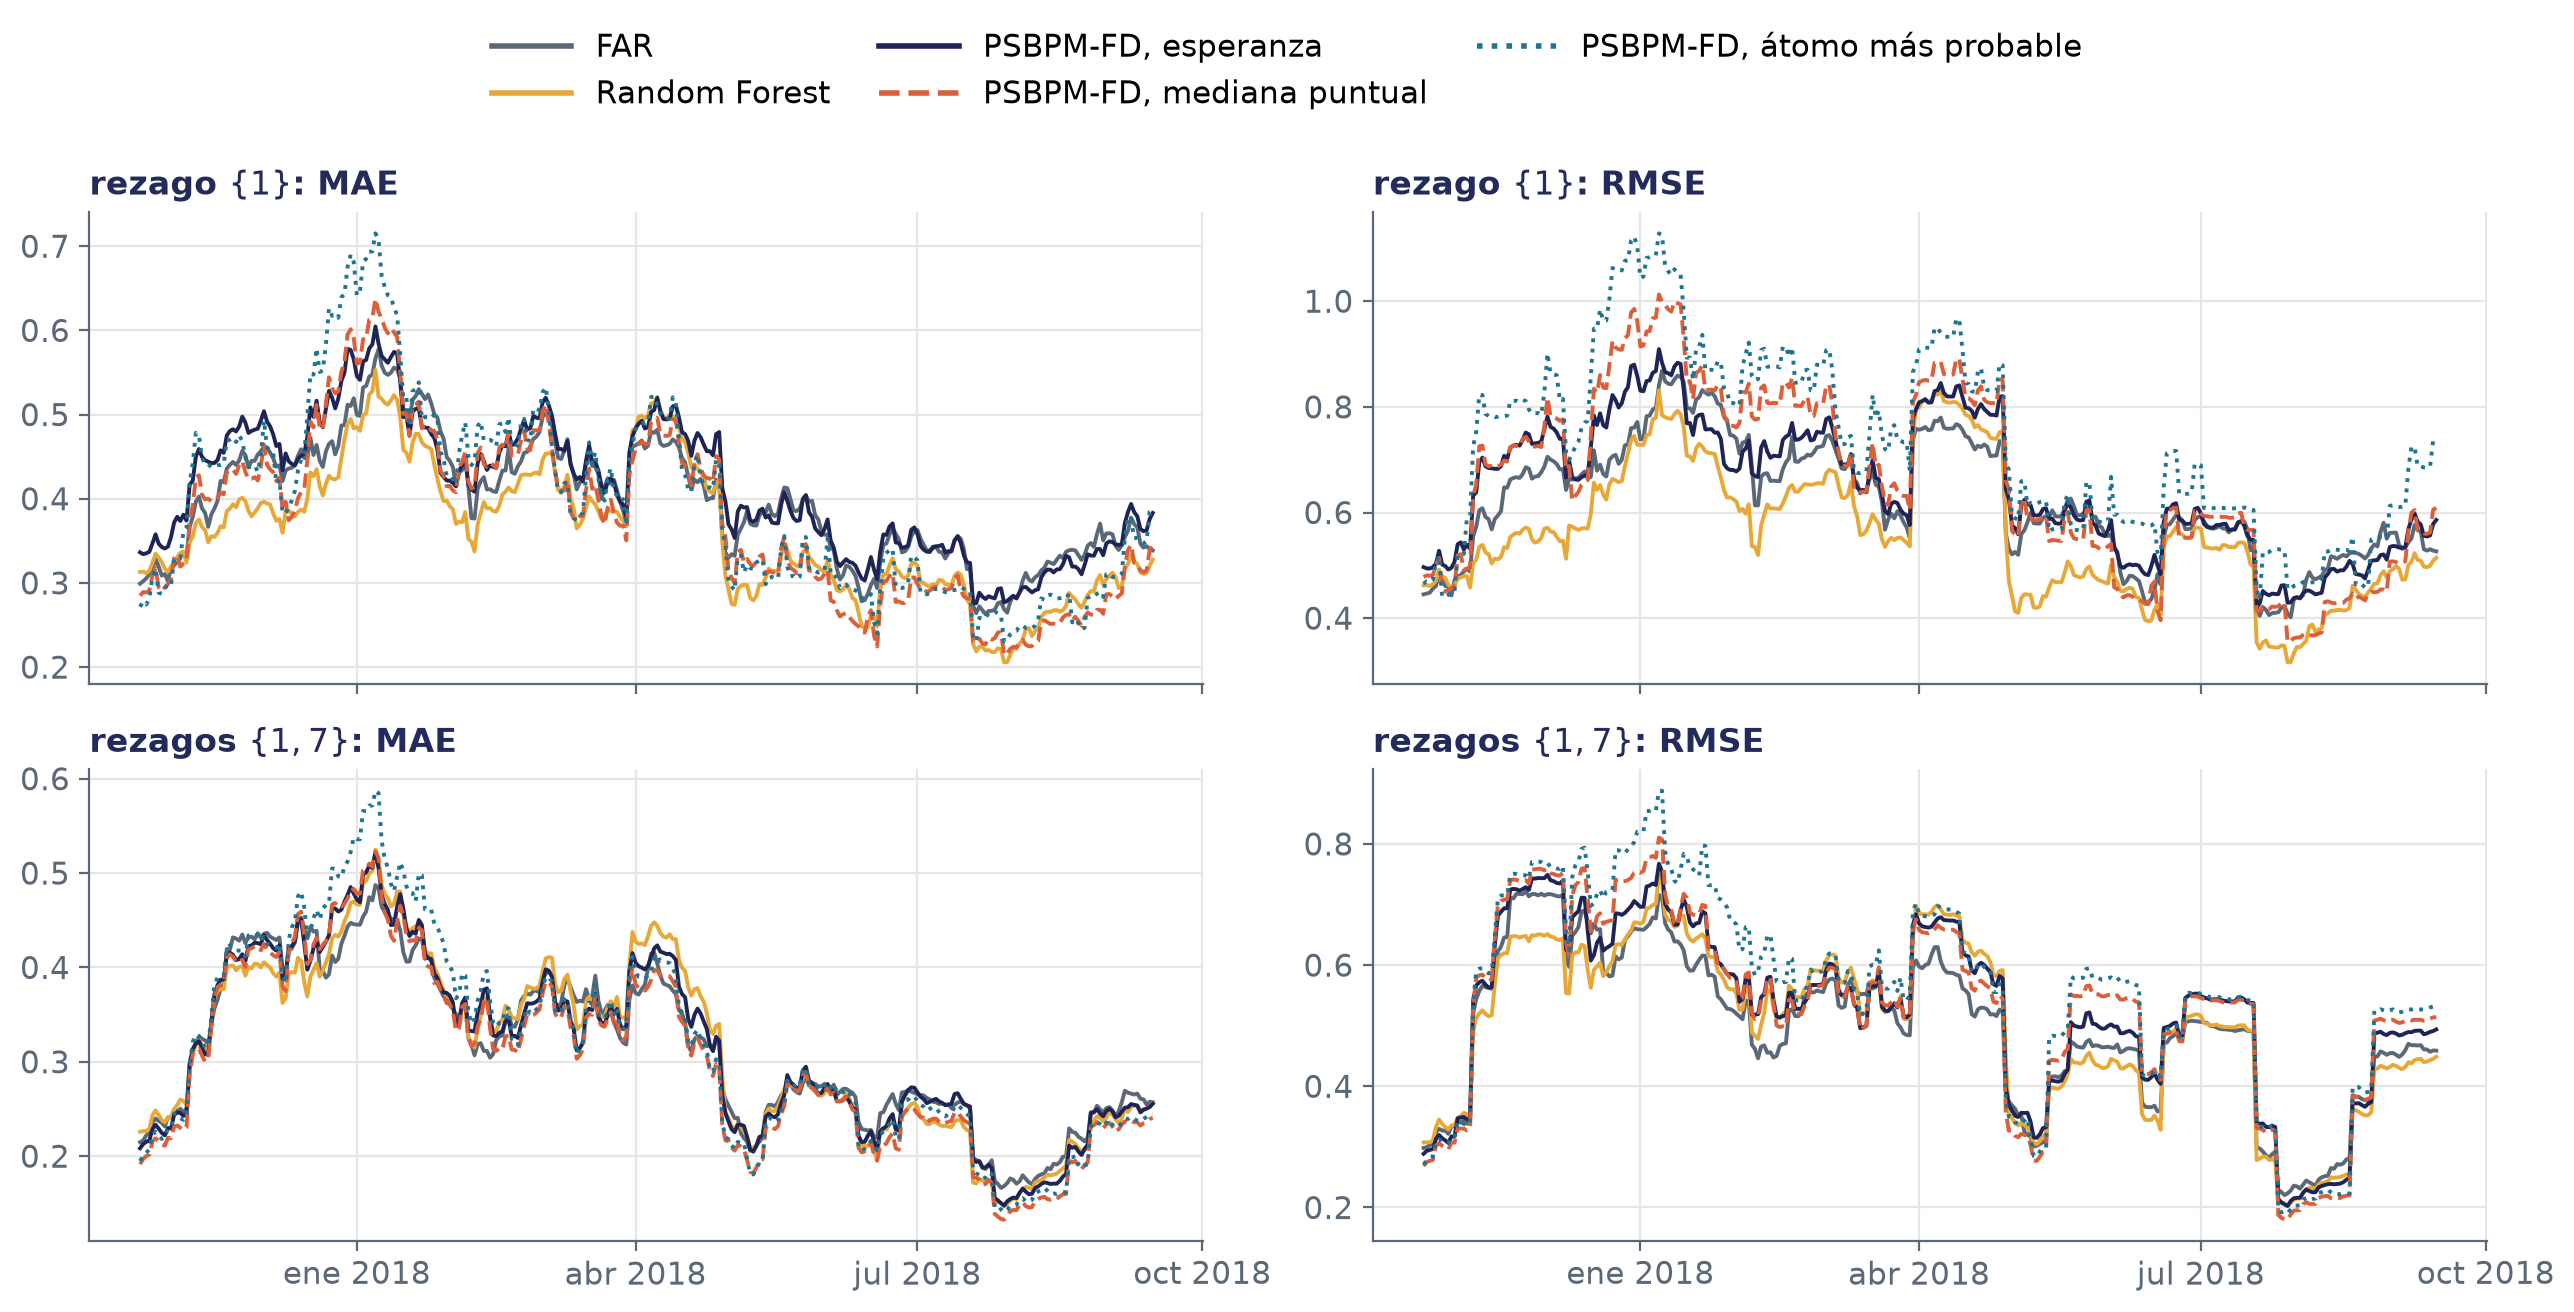
\includegraphics[width=\textwidth]{IMG/04_03/04_bloqueA_ventana_w30.png}
\caption{MAE y RMSE sobre la ventana móvil del bloque de prueba, con rezago $\{1\}$ (arriba) y rezagos $\{1,7\}$ (abajo) ($M = 10$, $w = 30$).}
\label{fig:apl_bloqueA_ventana}
\end{figure}

La Figura~\ref{fig:apl_bloqueA_ventana} muestra que todos los modelos suben y bajan juntos, y el máximo se alcanza en las ventanas que contienen el período de fiestas de fin de año, donde se concentran los feriados que ningún rezago anuncia. Con el rezago de un día las curvas se separan, el Random Forest queda debajo en buena parte del bloque y el átomo más probable se despega hacia arriba en RMSE en los meses de invierno; con ambos rezagos las curvas de todos los modelos casi se superponen, que es la imagen en el tiempo de lo que muestran los cuadros, es decir, la información sobre el tipo de día elimina las diferencias entre métodos en el error puntual.

\subsection{Intervalos de predicción}
\label{04_03_02_intervalos}

Los Cuadros~\ref{tab:apl_bloqueB_winkler} y~\ref{tab:apl_bloqueB_picp} resumen el Winkler, el MPIW, el PICP y el PICPB de las tres construcciones del PSBPM-FD y de la banda gaussiana del FAR, al nivel nominal de $95\%$.

% Fuente: 99_resumen_bloqueB_min_max_prom.csv y 81_ventana_bloqueB_w30.csv del _05.
\begin{table}[H]
\centering\small
\setlength{\tabcolsep}{3.5pt}
\caption{Winkler y MPIW en el bloque de prueba del tráfico ($M = 10$). En negrita el menor Winkler de cada fila.}
\label{tab:apl_bloqueB_winkler}
\begin{tabular}{l cccc cccc}
\hline
Rezagos & \multicolumn{4}{c}{Winkler} & \multicolumn{4}{c}{MPIW} \\
 & FAR & Equi. & HDR & Simult. & FAR & Equi. & HDR & Simult. \\
\hline
$\{1\}$ & 3.073 & 2.734 & \textbf{2.669} & 4.493 & 2.159 & 2.124 & 1.995 & 4.242 \\
$\{1,7\}$ & 3.052 & \textbf{2.707} & 2.714 & 3.549 & 1.602 & 1.752 & 1.689 & 3.011 \\
\hline
\end{tabular}
\end{table}

\begin{table}[H]
\centering\small
\setlength{\tabcolsep}{3.5pt}
\caption{PICP y PICPB en el bloque de prueba del tráfico ($M = 10$). Nominal $0.95$.}
\label{tab:apl_bloqueB_picp}
\begin{tabular}{l cccc cccc}
\hline
Rezagos & \multicolumn{4}{c}{PICP} & \multicolumn{4}{c}{PICPB} \\
 & FAR & Equi. & HDR & Simult. & FAR & Equi. & HDR & Simult. \\
\hline
$\{1\}$ & 0.950 & 0.961 & 0.960 & 0.991 & 0.721 & 0.731 & 0.742 & 0.942 \\
$\{1,7\}$ & 0.930 & 0.956 & 0.955 & 0.983 & 0.675 & 0.754 & 0.746 & 0.917 \\
\hline
\end{tabular}
\end{table}

En los intervalos el PSBPM-FD supera al FAR en las dos especificaciones. Las bandas puntuales, equi-colas y de máxima densidad, bajan el Winkler del FAR en un $11\%$ a $13\%$ y cubren el $96\%$ del dominio, por sobre el $93\%$ a $95\%$ del FAR. La ganancia no depende del rezago semanal, a diferencia del error puntual, ya que aun cuando la información resuelve el tipo de día, la incertidumbre alrededor del perfil sigue cambiando de un origen a otro, y una banda de ancho fijo no puede seguirla. Ninguna banda puntual cubre la curva completa con la frecuencia nominal, porque su PICPB queda entre $0.68$ y $0.75$; la simultánea, la única construida para esa cobertura, la alcanza casi ($0.92$ a $0.94$) al precio de casi duplicar el ancho, y por eso pierde el Winkler.

\begin{table}[H]
\centering\small
\setlength{\tabcolsep}{3pt}
\caption{Cambio relativo del Winkler y del MPIW respecto del FAR por construcción. Negativo es mejor que el FAR.}
\label{tab:apl_bloqueB_ganancia}
\begin{tabular}{l cc cc cc}
\hline
Rezagos & \multicolumn{2}{c}{Equi-colas} & \multicolumn{2}{c}{Máxima densidad} & \multicolumn{2}{c}{Simultánea} \\
 & Winkler & MPIW & Winkler & MPIW & Winkler & MPIW \\
\hline
$\{1\}$ & $-11.0\%$ & $-1.6\%$ & $-13.2\%$ & $-7.6\%$ & $+46.2\%$ & $+96.5\%$ \\
$\{1,7\}$ & $-11.3\%$ & $+9.4\%$ & $-11.1\%$ & $+5.4\%$ & $+16.3\%$ & $+88.0\%$ \\
\hline
\end{tabular}
\end{table}

El Cuadro~\ref{tab:apl_bloqueB_ganancia} muestra que la composición de la ganancia cambia con la información. Con el rezago de un día las bandas del PSBPM-FD son más angostas que la del FAR y además cubren más, y la de máxima densidad es la más angosta de todas ($-7.6\%$), porque cuando la predictiva tiene dos comportamientos reparte su masa entre ellos en lugar de gastarla en el valle intermedio, como hace la equi-colas. Con ambos rezagos las bandas son un $5\%$ a $9\%$ más anchas que la del FAR y ganan por cobertura, porque la del FAR, al estrecharse con la mejor información, queda corta ($0.93$ de PICP) en los días que el rezago semanal no anuncia. La máxima densidad coincide entonces con la equi-colas, como en los escenarios unimodales de la simulación.

% Fuente: 81_ventana_bloqueB_w30.csv (test, w = 30).
\begin{table}[H]
\centering\small
\setlength{\tabcolsep}{3.5pt}
\caption{Ventanas de prueba ganadas por Winkler.}
\label{tab:apl_bloqueB_ventanas}
\begin{tabular}{l cccc ccc}
\hline
Rezagos & \multicolumn{4}{c}{La mejor banda} & \multicolumn{3}{c}{Gana al FAR} \\
 & FAR & Equi. & HDR & Simult. & Equi. & HDR & Simult. \\
\hline
$\{1\}$ & 3\% & 21\% & 76\% & 0\% & 93\% & 93\% & 4\% \\
$\{1,7\}$ & 22\% & 26\% & 52\% & 0\% & 76\% & 75\% & 12\% \\
\hline
\end{tabular}
\end{table}

Las bandas puntuales superan al FAR en el $93\%$ de las ventanas con el rezago de un día y en tres de cada cuatro con ambos rezagos (Cuadro~\ref{tab:apl_bloqueB_ventanas}), y la de máxima densidad es la mejor de todas en el $76\%$ y el $52\%$ de ellas. La simultánea no es la mejor en ninguna ventana.

% Fuente: 81_ventana_bloqueB_w30.csv de 101 y 102 (test); figura en docs/IMG/04_03.
\begin{figure}[H]
\centering
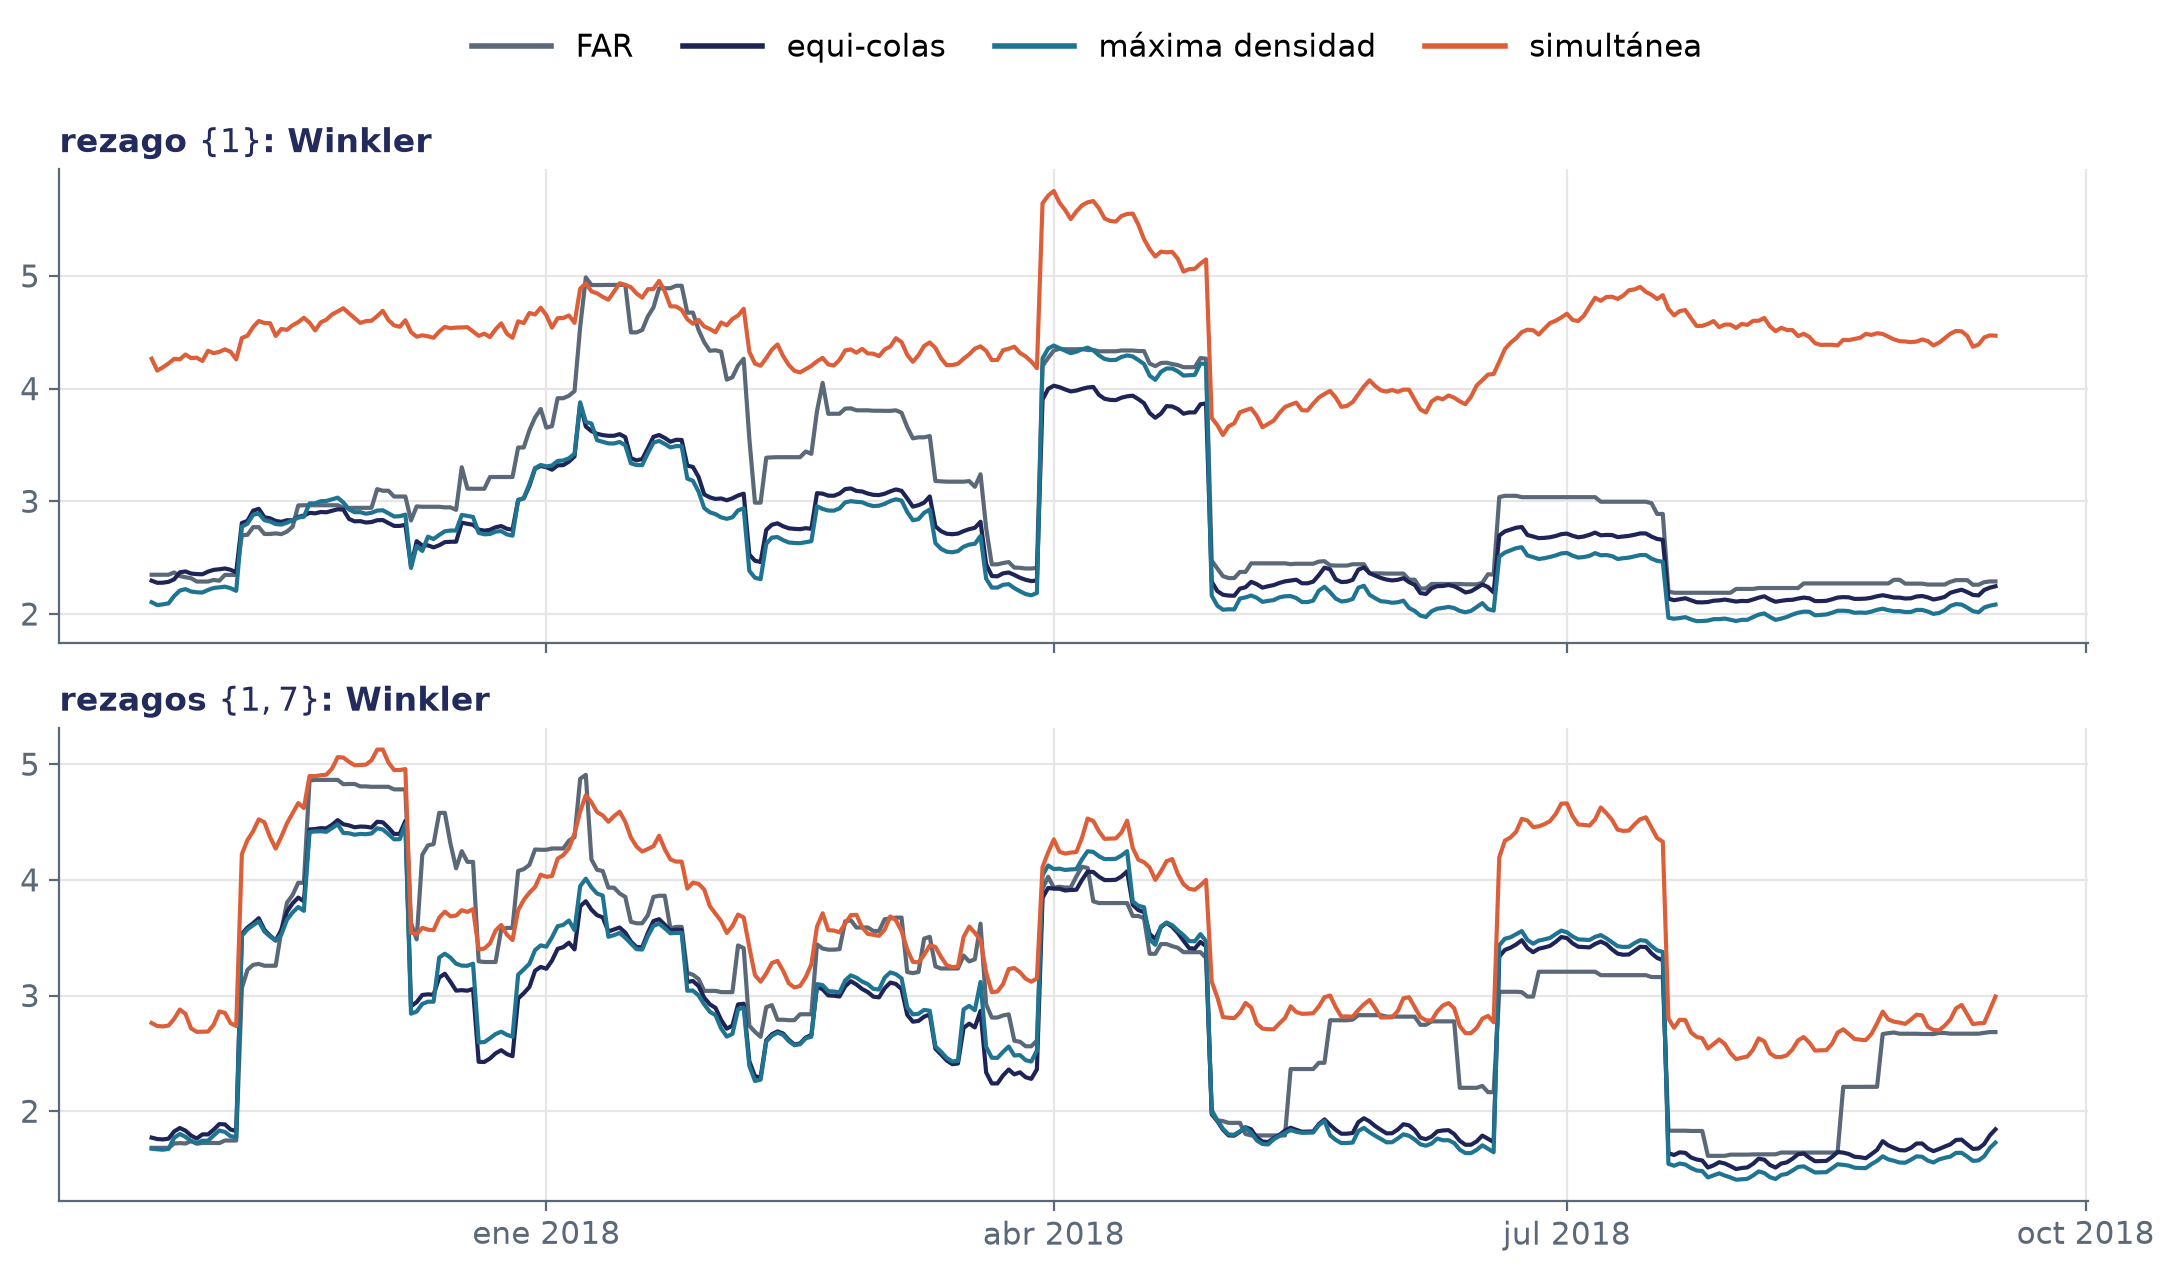
\includegraphics[width=\textwidth]{IMG/04_03/04_bloqueB_ventana_w30.png}
\caption{Winkler sobre la ventana móvil del bloque de prueba, con rezago $\{1\}$ (arriba) y rezagos $\{1,7\}$ (abajo) ($M = 10$, $w = 30$).}
\label{fig:apl_bloqueB_ventana}
\end{figure}

La Figura~\ref{fig:apl_bloqueB_ventana} muestra el Winkler a lo largo del bloque de prueba. En las dos especificaciones las bandas puntuales del PSBPM-FD quedan bajo el FAR en la mayor parte de las ventanas, y la diferencia es mayor en las del invierno, que incluyen el período de fiestas de fin de año, donde el Winkler del FAR aumenta por los días que su banda no cubre. Con ambos rezagos hay tramos, en abril y en julio, en que la banda del PSBPM-FD queda por encima del FAR, y son los que bajan su fracción de ventanas ganadas al $76\%$.\\

% Fuente: banda_funcional_psbp.npz del _04 (li, ls, hdr_L, hdr_U, li/ls_simultanea) y MPIW del FAR de 81_*.
\begin{figure}[H]
\centering
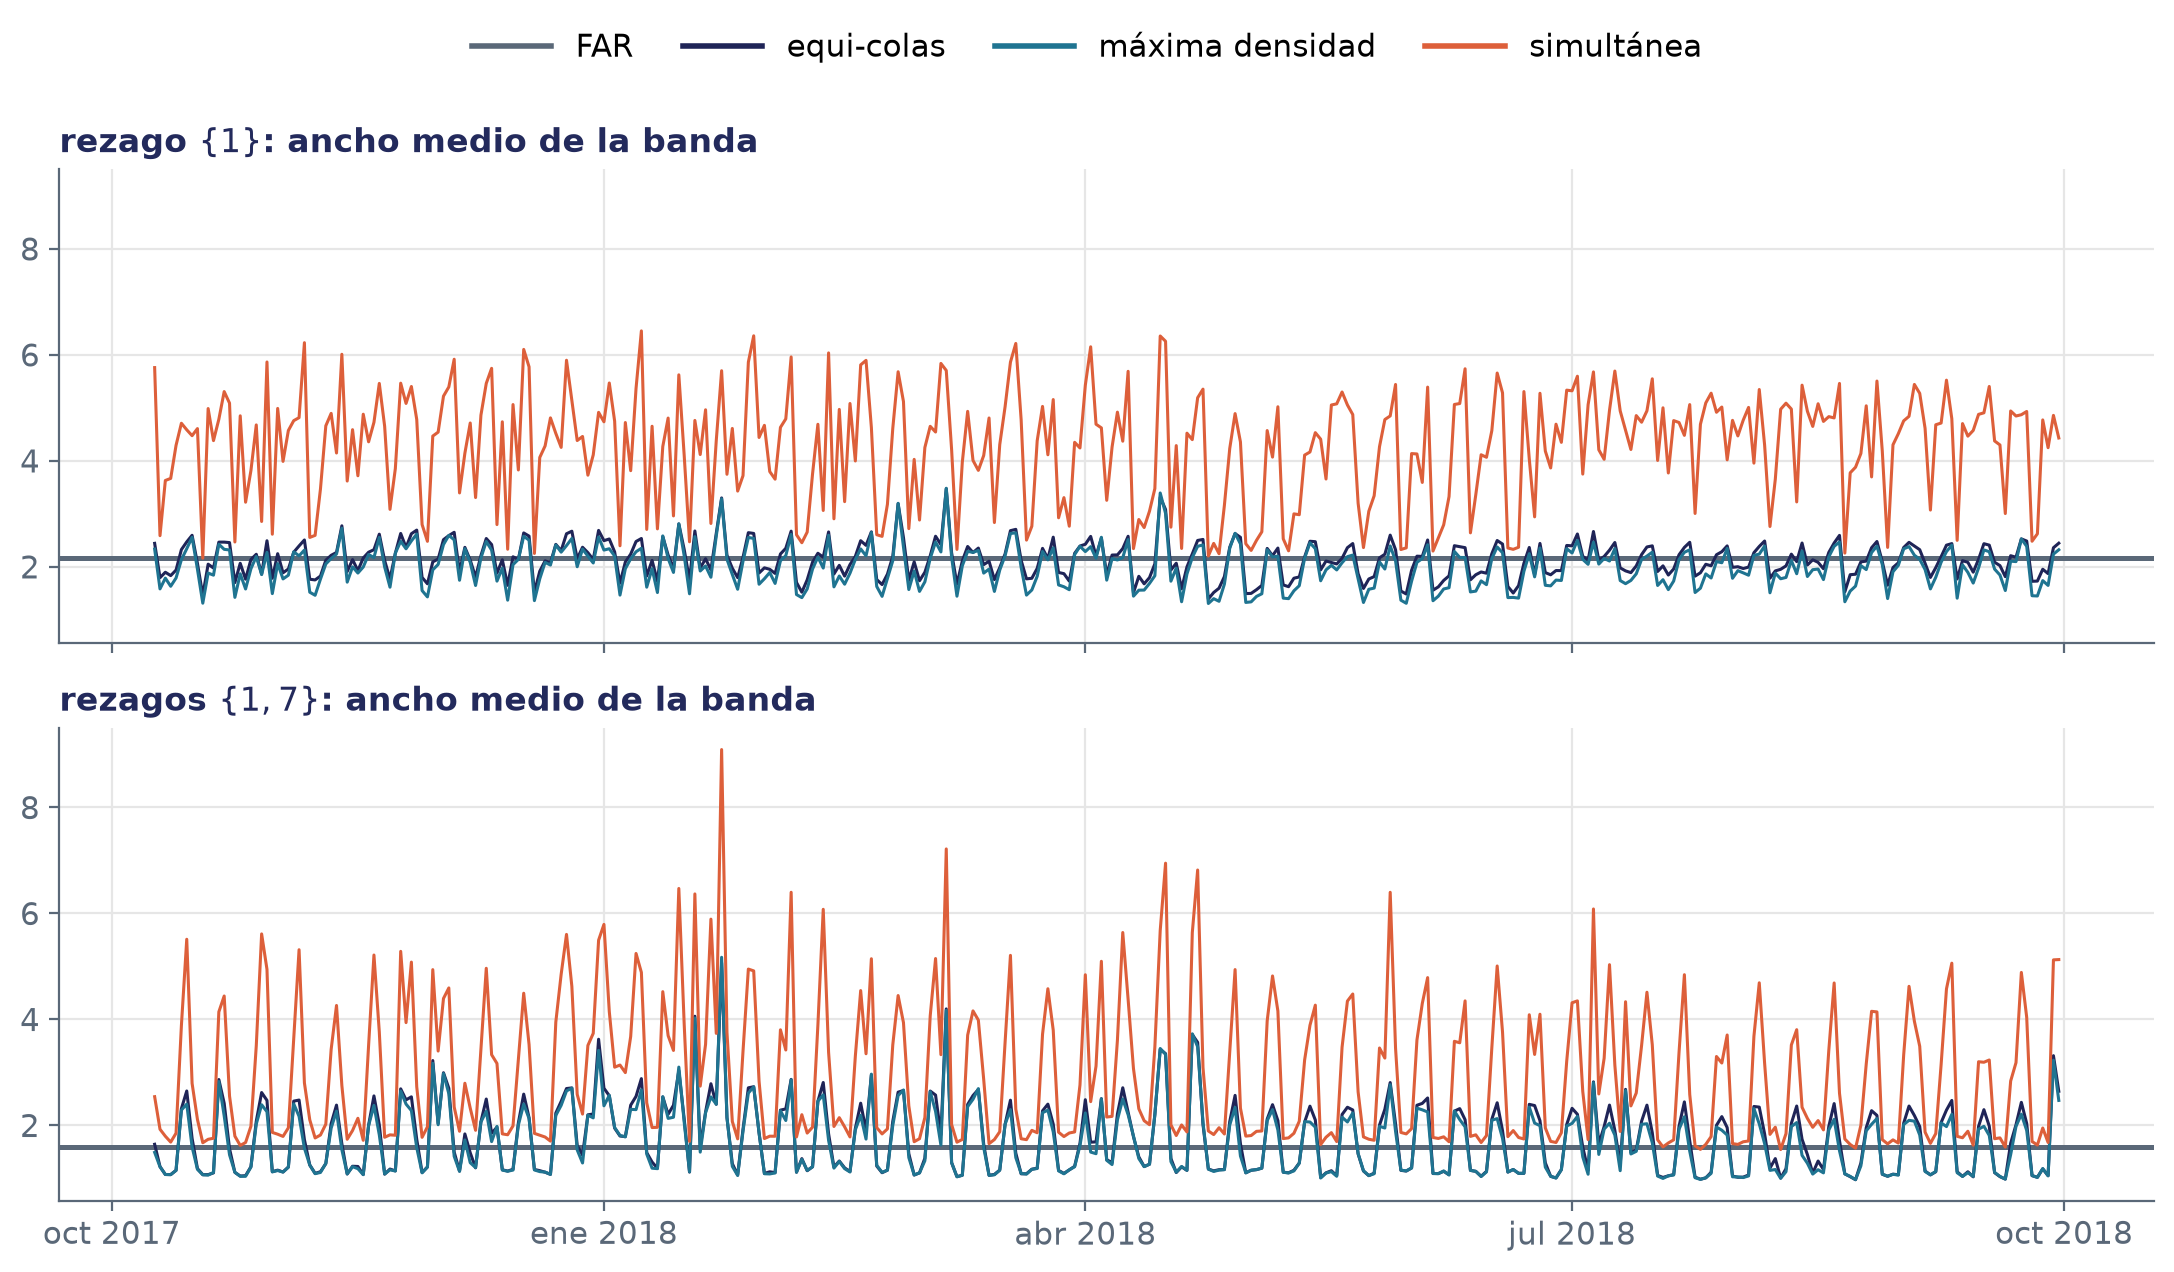
\includegraphics[width=\textwidth]{IMG/04_03/04_bloqueB_ancho.png}
\caption{Ancho medio de la banda en cada origen de prueba de las tres construcciones del PSBPM-FD y ancho fijo del FAR, con rezago $\{1\}$ (arriba) y rezagos $\{1,7\}$ (abajo) ($M = 10$).}
\label{fig:apl_bloqueB_ancho}
\end{figure}

La Figura~\ref{fig:apl_bloqueB_ancho} muestra que el ancho de la banda del FAR es el mismo en todos los orígenes, mientras que el del PSBPM-FD cambia con el tipo de día. Con ambos rezagos la banda equi-colas es más angosta que la del FAR en el $71\%$ de los días laborables, con un ancho medio de $1.48$ frente a $1.60$, y más ancha en el $96\%$ de los no laborables, con $2.34$, que son los días en que el rezago semanal ya no decide el perfil. Con el rezago de un día el patrón es menos marcado ($2.06$ en los laborables y $2.34$ en los no laborables, frente a $2.16$ del FAR), porque la predictiva ya reparte su masa entre los dos perfiles en la mayoría de los días.

\subsection{Comportamientos predictivos}
\label{04_03_03_comportamientos}

El Cuadro~\ref{tab:apl_K} resume cuántos comportamientos declara el modelo en el bloque de prueba con cada especificación.

% Fuente: 102_K_por_M.csv del barrido (bloque test, M = 10).
\begin{table}[H]
\centering\small
\setlength{\tabcolsep}{3.5pt}
\caption{Distribución de $K_t$ en el bloque de prueba del tráfico ($M = 10$).}
\label{tab:apl_K}
\begin{tabular}{l c ccc}
\hline
Rezagos & Orígenes & $K_t = 1$ & $K_t = 2$ & $K_t \ge 3$ \\
\hline
$\{1\}$ & 357 & 28.3\% & 71.7\% & 0.0\% \\
$\{1,7\}$ & 357 & 64.1\% & 35.0\% & 0.8\% \\
\hline
\end{tabular}
\end{table}

Con el rezago de un día el modelo declara dos comportamientos en el $72\%$ de los orígenes de prueba, y con ambos rezagos esa fracción baja a la mitad. A diferencia de la simulación, aquí no hay un régimen verdadero con el que contrastar los comportamientos, pero el calendario lo reemplaza, porque el tipo de día es el estado que decide el perfil y no entra al modelo. El Cuadro~\ref{tab:apl_K_calendario} cruza la presencia de más de un comportamiento con el día predicho.

% Fuente: 65_comportamientos_calendario.csv de 101 y 102 (test, 357 orígenes; 51 por día de la semana).
\begin{table}[H]
\centering\small
\caption{Fracción de orígenes de prueba con más de un comportamiento ($K_t \ge 2$) según el día predicho, con y sin el rezago de una semana ($M = 10$).}
\label{tab:apl_K_calendario}
\begin{tabular}{l c cc}
\hline
Día predicho & Orígenes & $\{1\}$ & $\{1,7\}$ \\
\hline
Lunes     & 51  & 100\% & 49\% \\
Martes    & 51  & 41\%  & 12\% \\
Miércoles & 51  & 57\%  & 4\%  \\
Jueves    & 51  & 49\%  & 6\%  \\
Viernes   & 51  & 75\%  & 8\%  \\
Sábado    & 51  & 94\%  & 90\% \\
Domingo   & 51  & 86\%  & 82\% \\
\hline
Laborables    & 244 & 64\% & 14\% \\
No laborables (fin de semana y feriados) & 113 & 89\% & 82\% \\
\hline
\end{tabular}
\end{table}

 Con el rezago de un día hay más de un comportamiento en todos los días de la semana, y sobre todo los lunes y los sábados, los días en que el perfil cambia respecto del anterior, ya que la curva del domingo no distingue un lunes laborable de un lunes feriado, y la del viernes no anuncia el cambio al fin de semana con la claridad suficiente para que la mezcla excluya el perfil laborable. Con ambos rezagos los comportamientos desaparecen de martes a viernes, donde quedan entre un $4\%$ y un $12\%$ de los orígenes, porque la curva de la semana anterior fija el perfil, y la predictiva se vuelve unimodal. Se mantienen en los días no laborables y la mitad de los lunes, que son los días en que el rezago semanal no basta, porque los feriados caen en días que la semana anterior fueron laborables, y los fines de semana tienen una variabilidad propia, de salidas y eventos, que ningún rezago resuelve. De los 256 orígenes con más de un comportamiento en la primera especificación, 139 pasan a tener uno solo en la segunda, mientras que solo 11 hacen el camino inverso. La mezcla no genera comportamientos donde la información alcanza para decidir el perfil, y los conserva donde no alcanza, que es lo que se espera de pesos que dependen de las covariables.

% Fuente: comportamientos_psbp.npz y banda_funcional_psbp.npz del _04 de 101 y 102, curva suavizada (theta @ phi^T).
\begin{figure}[H]
\centering
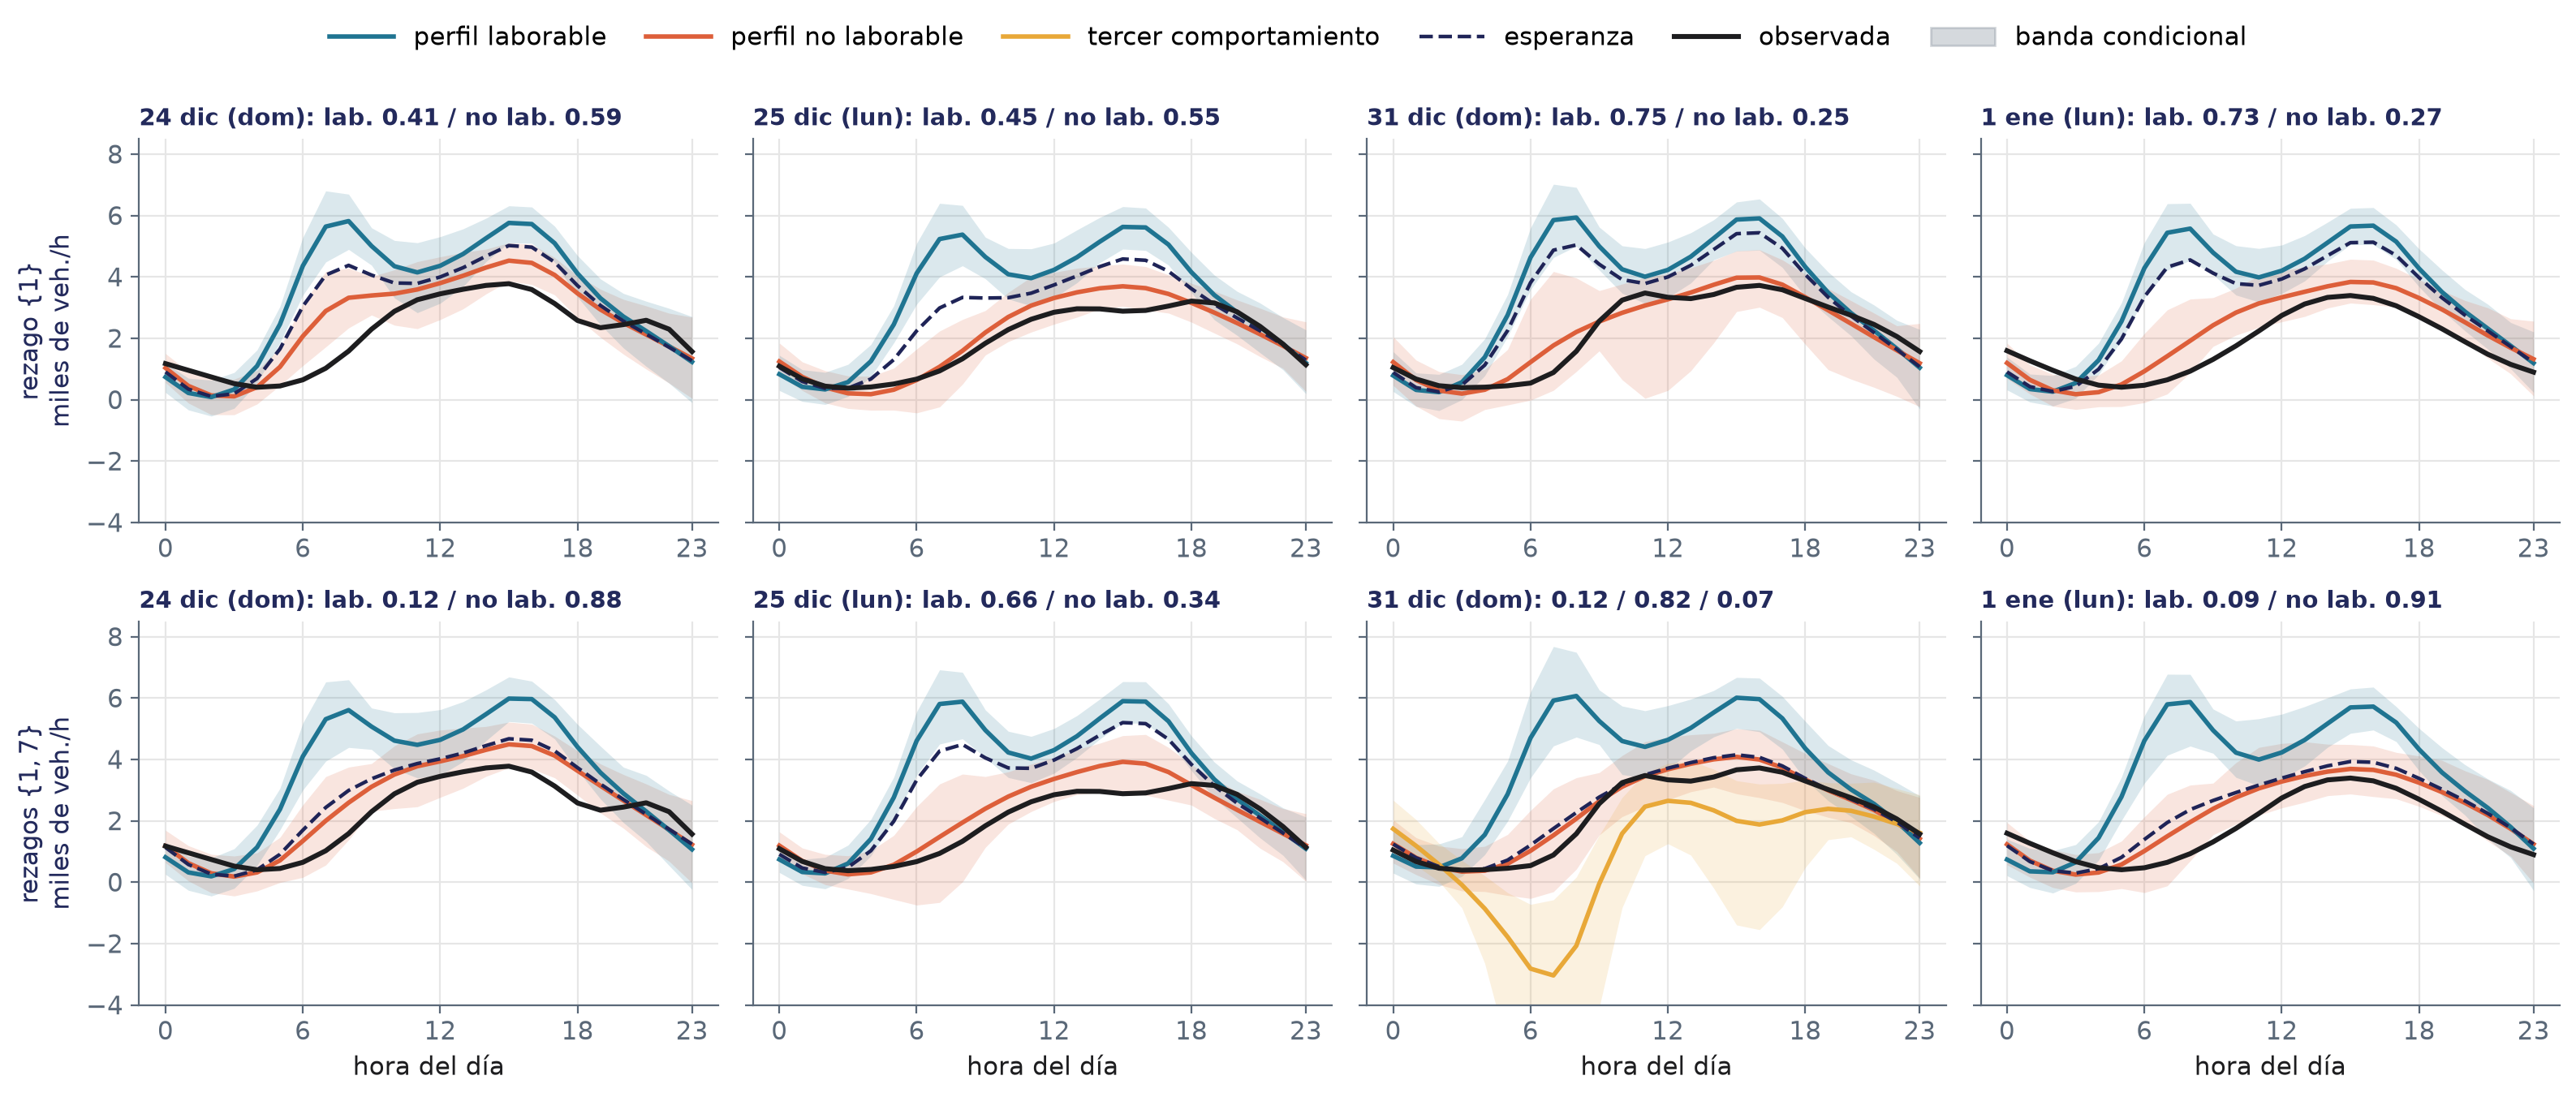
\includegraphics[width=\textwidth]{IMG/04_03/04_ventana_detalle.png}
\caption{Cuatro orígenes de la ventana de detalle, con rezago $\{1\}$ (arriba) y rezagos $\{1,7\}$ (abajo) ($M = 10$): curva observada, esperanza y, por comportamiento, curva típica y banda condicional. Los comportamientos se nombran por su perfil y el título da la probabilidad de cada uno; con tres comportamientos, en orden de nivel.}
\label{fig:apl_ventana_detalle}
\end{figure}

La Figura~\ref{fig:apl_ventana_detalle} muestra cuatro días de la ventana de detalle. En los orígenes con dos comportamientos, uno tiene la forma del día laborable, con sus dos horas punta, y el otro la del fin de semana, con un solo máximo al mediodía, y la esperanza queda entre ambos, en una curva con horas punta atenuadas que no corresponde a ningún día. Con el rezago de un día, el 24 y el 25 de diciembre el comportamiento más probable es el no laborable y la curva observada lo sigue, aunque con probabilidades cercanas a un medio. El 31 de diciembre y el 1 de enero el más probable es el laborable y la curva observada sigue al comportamiento minoritario, que el modelo mantiene con una probabilidad cercana a un cuarto y cuya banda la contiene, lo que corresponde al caso en que una predictiva con más de un comportamiento ofrece una opción que el promedio no tiene.\\

Con ambos rezagos la masa se desplaza hacia el perfil correcto, de modo que el no laborable recibe $0.88$ el 24 de diciembre, $0.82$ el 31 y $0.91$ el 1 de enero, porque el lunes anterior fue Navidad y el rezago semanal anuncia el feriado. La excepción es la propia Navidad, un lunes precedido por un lunes laborable, en que el rezago semanal empuja la masa hacia el perfil laborable ($0.66$) y la curva observada sigue al minoritario. La información del rezago semanal resuelve el tipo de día cuando la semana anterior lo anuncia, y no cuando no lo anuncia. Los diez orígenes de la ventana se muestran en el Anexo~\ref{aneC_00_00_trafico}.\\

Los comportamientos funcionan, por tanto, como un agrupamiento de la curva siguiente por tipo de día, el estado latente que el calendario registra y que no entra al modelo. Para medirlo, en cada origen con dos comportamientos se identifica el de perfil no laborable como el de menor nivel medio y se lo cruza con el día predicho (Cuadro~\ref{tab:apl_K_tipo}).

% Fuente: comportamientos_psbp.npz de 101 y 102 (test, K = 2) y 65_comportamientos_calendario.csv; el perfil
% no laborable es el comportamiento de menor nivel medio; "observada más cerca" = menor distancia L2 a la curva típica.
\begin{table}[H]
\centering\small
\setlength{\tabcolsep}{4pt}
\caption{Comportamientos y tipo de día en los orígenes de prueba con dos comportamientos ($M = 10$). Fracción en que el comportamiento más probable corresponde al tipo de día predicho, probabilidad media de ese comportamiento y fracción en que la curva observada queda más cerca de él que del otro.}
\label{tab:apl_K_tipo}
\begin{tabular}{l l c ccc}
\hline
Rezagos & Día predicho & Orígenes & Más probable & Probabilidad & Observada \\
 & & & corresponde & media & más cerca \\
\hline
$\{1\}$   & Laborable    & 155 & 95.5\% & 0.80 & 96.8\% \\
          & No laborable & 101 & 55.4\% & 0.55 & 96.0\% \\
          & Todos        & 256 & 79.7\% & 0.70 & 96.5\% \\
\hline
$\{1,7\}$ & Laborable    & 35  & 65.7\% & 0.63 & 94.3\% \\
          & No laborable & 90  & 95.6\% & 0.83 & 97.8\% \\
          & Todos        & 125 & 87.2\% & 0.77 & 96.8\% \\
\hline
\end{tabular}
\end{table}

En las dos especificaciones la curva observada queda más cerca del comportamiento que corresponde a su tipo de día en el $96\%$ a $97\%$ de los orígenes, de modo que los dos comportamientos corresponden a los dos tipos de día. Lo que cambia con la información no es el agrupamiento sino la probabilidad que recibe cada grupo. Con el rezago de un día el modelo acierta el tipo de los días laborables, porque la mayoría siguen a otro laborable, pero en los no laborables el comportamiento correcto es el más probable solo en el $55\%$ de los casos, cerca de lo que daría el azar. Con el rezago semanal ese acierto sube al $96\%$, con una probabilidad media de $0.83$. Los pocos laborables que conservan dos comportamientos son sobre todo lunes (20 de 35), en que el rezago de un día viene de un fin de semana, y en ellos el acierto baja al $66\%$.

\subsection{Predicción por comportamiento}
\label{04_03_04_pronostico}

Los Cuadros~\ref{tab:apl_pronostico_101} y~\ref{tab:apl_pronostico_102} resumen el error del pronóstico por comportamiento y de su cota frente a la esperanza y a las referencias, sobre todos los orígenes de prueba y sobre los que tienen más de un comportamiento. Como en la simulación, se promedia sobre los orígenes y no sobre las ventanas, porque el subconjunto con más de un comportamiento no es contiguo, y por eso las cifras difieren en la tercera decimal de las del error puntual.

% Fuente: 113_opciones_por_origen.csv (m10, test, opción "tipica") y 119_resumen_opciones_por_M.csv;
% MAE = media por origen, RMSE = raíz de la media de cuadrados por origen.
\begin{table}[H]
\centering\small
\setlength{\tabcolsep}{4pt}
\caption{Pronóstico por comportamiento en el bloque de prueba del tráfico con rezago $\{1\}$ ($M = 10$), sobre todos los orígenes y sobre los que tienen más de un comportamiento.}
\label{tab:apl_pronostico_101}
\begin{tabular}{l cc cc}
\hline
& \multicolumn{2}{c}{Todos ($n = 357$)} & \multicolumn{2}{c}{$K_t \ge 2$ ($n = 256$)} \\
 & MAE & RMSE & MAE & RMSE \\
\hline
Pronóstico por comportamiento & 0.386 & 0.719 & 0.417 & 0.779 \\
Cota (mejor comportamiento) & 0.269 & 0.432 & 0.254 & 0.382 \\
Esperanza & 0.409 & 0.650 & 0.449 & 0.688 \\
FAR & 0.390 & 0.620 & 0.431 & 0.654 \\
Random Forest & 0.357 & 0.568 & 0.384 & 0.590 \\
\hline
El pronóstico gana al FAR & \multicolumn{2}{c}{56\%} & \multicolumn{2}{c}{66\%} \\
El pronóstico gana al Random Forest & \multicolumn{2}{c}{51\%} & \multicolumn{2}{c}{58\%} \\
La cota gana al FAR & \multicolumn{2}{c}{70\%} & \multicolumn{2}{c}{85\%} \\
La cota gana al Random Forest & \multicolumn{2}{c}{64\%} & \multicolumn{2}{c}{75\%} \\
Acierto (el mejor es el más probable) & \multicolumn{2}{c}{85\%} & \multicolumn{2}{c}{79\%} \\
\hline
\end{tabular}
\end{table}

\begin{table}[H]
\centering\small
\setlength{\tabcolsep}{4pt}
\caption{Pronóstico por comportamiento en el bloque de prueba del tráfico con rezagos $\{1,7\}$ ($M = 10$), sobre todos los orígenes y sobre los que tienen más de un comportamiento.}
\label{tab:apl_pronostico_102}
\begin{tabular}{l cc cc}
\hline
& \multicolumn{2}{c}{Todos ($n = 357$)} & \multicolumn{2}{c}{$K_t \ge 2$ ($n = 128$)} \\
 & MAE & RMSE & MAE & RMSE \\
\hline
Pronóstico por comportamiento & 0.300 & 0.550 & 0.413 & 0.718 \\
Cota (mejor comportamiento) & 0.259 & 0.435 & 0.299 & 0.445 \\
Esperanza & 0.306 & 0.528 & 0.431 & 0.669 \\
FAR & 0.306 & 0.499 & 0.380 & 0.587 \\
Random Forest & 0.307 & 0.504 & 0.410 & 0.619 \\
\hline
El pronóstico gana al FAR & \multicolumn{2}{c}{61\%} & \multicolumn{2}{c}{56\%} \\
El pronóstico gana al Random Forest & \multicolumn{2}{c}{63\%} & \multicolumn{2}{c}{66\%} \\
La cota gana al FAR & \multicolumn{2}{c}{65\%} & \multicolumn{2}{c}{66\%} \\
La cota gana al Random Forest & \multicolumn{2}{c}{68\%} & \multicolumn{2}{c}{79\%} \\
Acierto (el mejor es el más probable) & \multicolumn{2}{c}{95\%} & \multicolumn{2}{c}{86\%} \\
\hline
\end{tabular}
\end{table}

El pronóstico por comportamiento elige, como en la simulación, uno de los perfiles posibles, y eso tiene un costo cuando elige mal. Con el rezago de un día baja el MAE de la esperanza en un $6\%$ sobre todos los orígenes y en un $7\%$ sobre los que tienen más de un comportamiento, queda al nivel del FAR y supera al FAR y al Random Forest en la mayoría de los orígenes con más de un comportamiento, pero es peor en RMSE que todas las alternativas, porque cuando acierta, su error es menor que el de la esperanza, y cuando elige el perfil incorrecto, el error es el de un día laborable predicho como fin de semana, o al revés, y el promedio cuadrático lo penaliza. Con ambos rezagos la mayoría de los orígenes tiene un solo comportamiento, el pronóstico coincide con la esperanza en ellos y sobre todos los orígenes es el mejor en MAE ($0.300$); en los orígenes que conservan más de un comportamiento, que son sobre todo fines de semana y feriados, el FAR queda por debajo.\\

La cota indica cuánto se puede ganar al elegir bien. Con el rezago de un día, en los orígenes con más de un comportamiento, la cota baja el MAE de la esperanza en un $43\%$ y queda bajo el Random Forest en tres de cada cuatro orígenes, de modo que entre las opciones que entrega el modelo casi siempre está la buena, y la pérdida se produce al elegirla según la probabilidad. Con ambos rezagos la distancia entre el pronóstico y la cota se reduce, porque la información que antes repartía la masa entre dos opciones ahora decide por una de ellas.

% Fuente: 115_ventana_modelos_w30.csv del _06 de 101 y 102 (test, opción "tipica").
\begin{figure}[H]
\centering
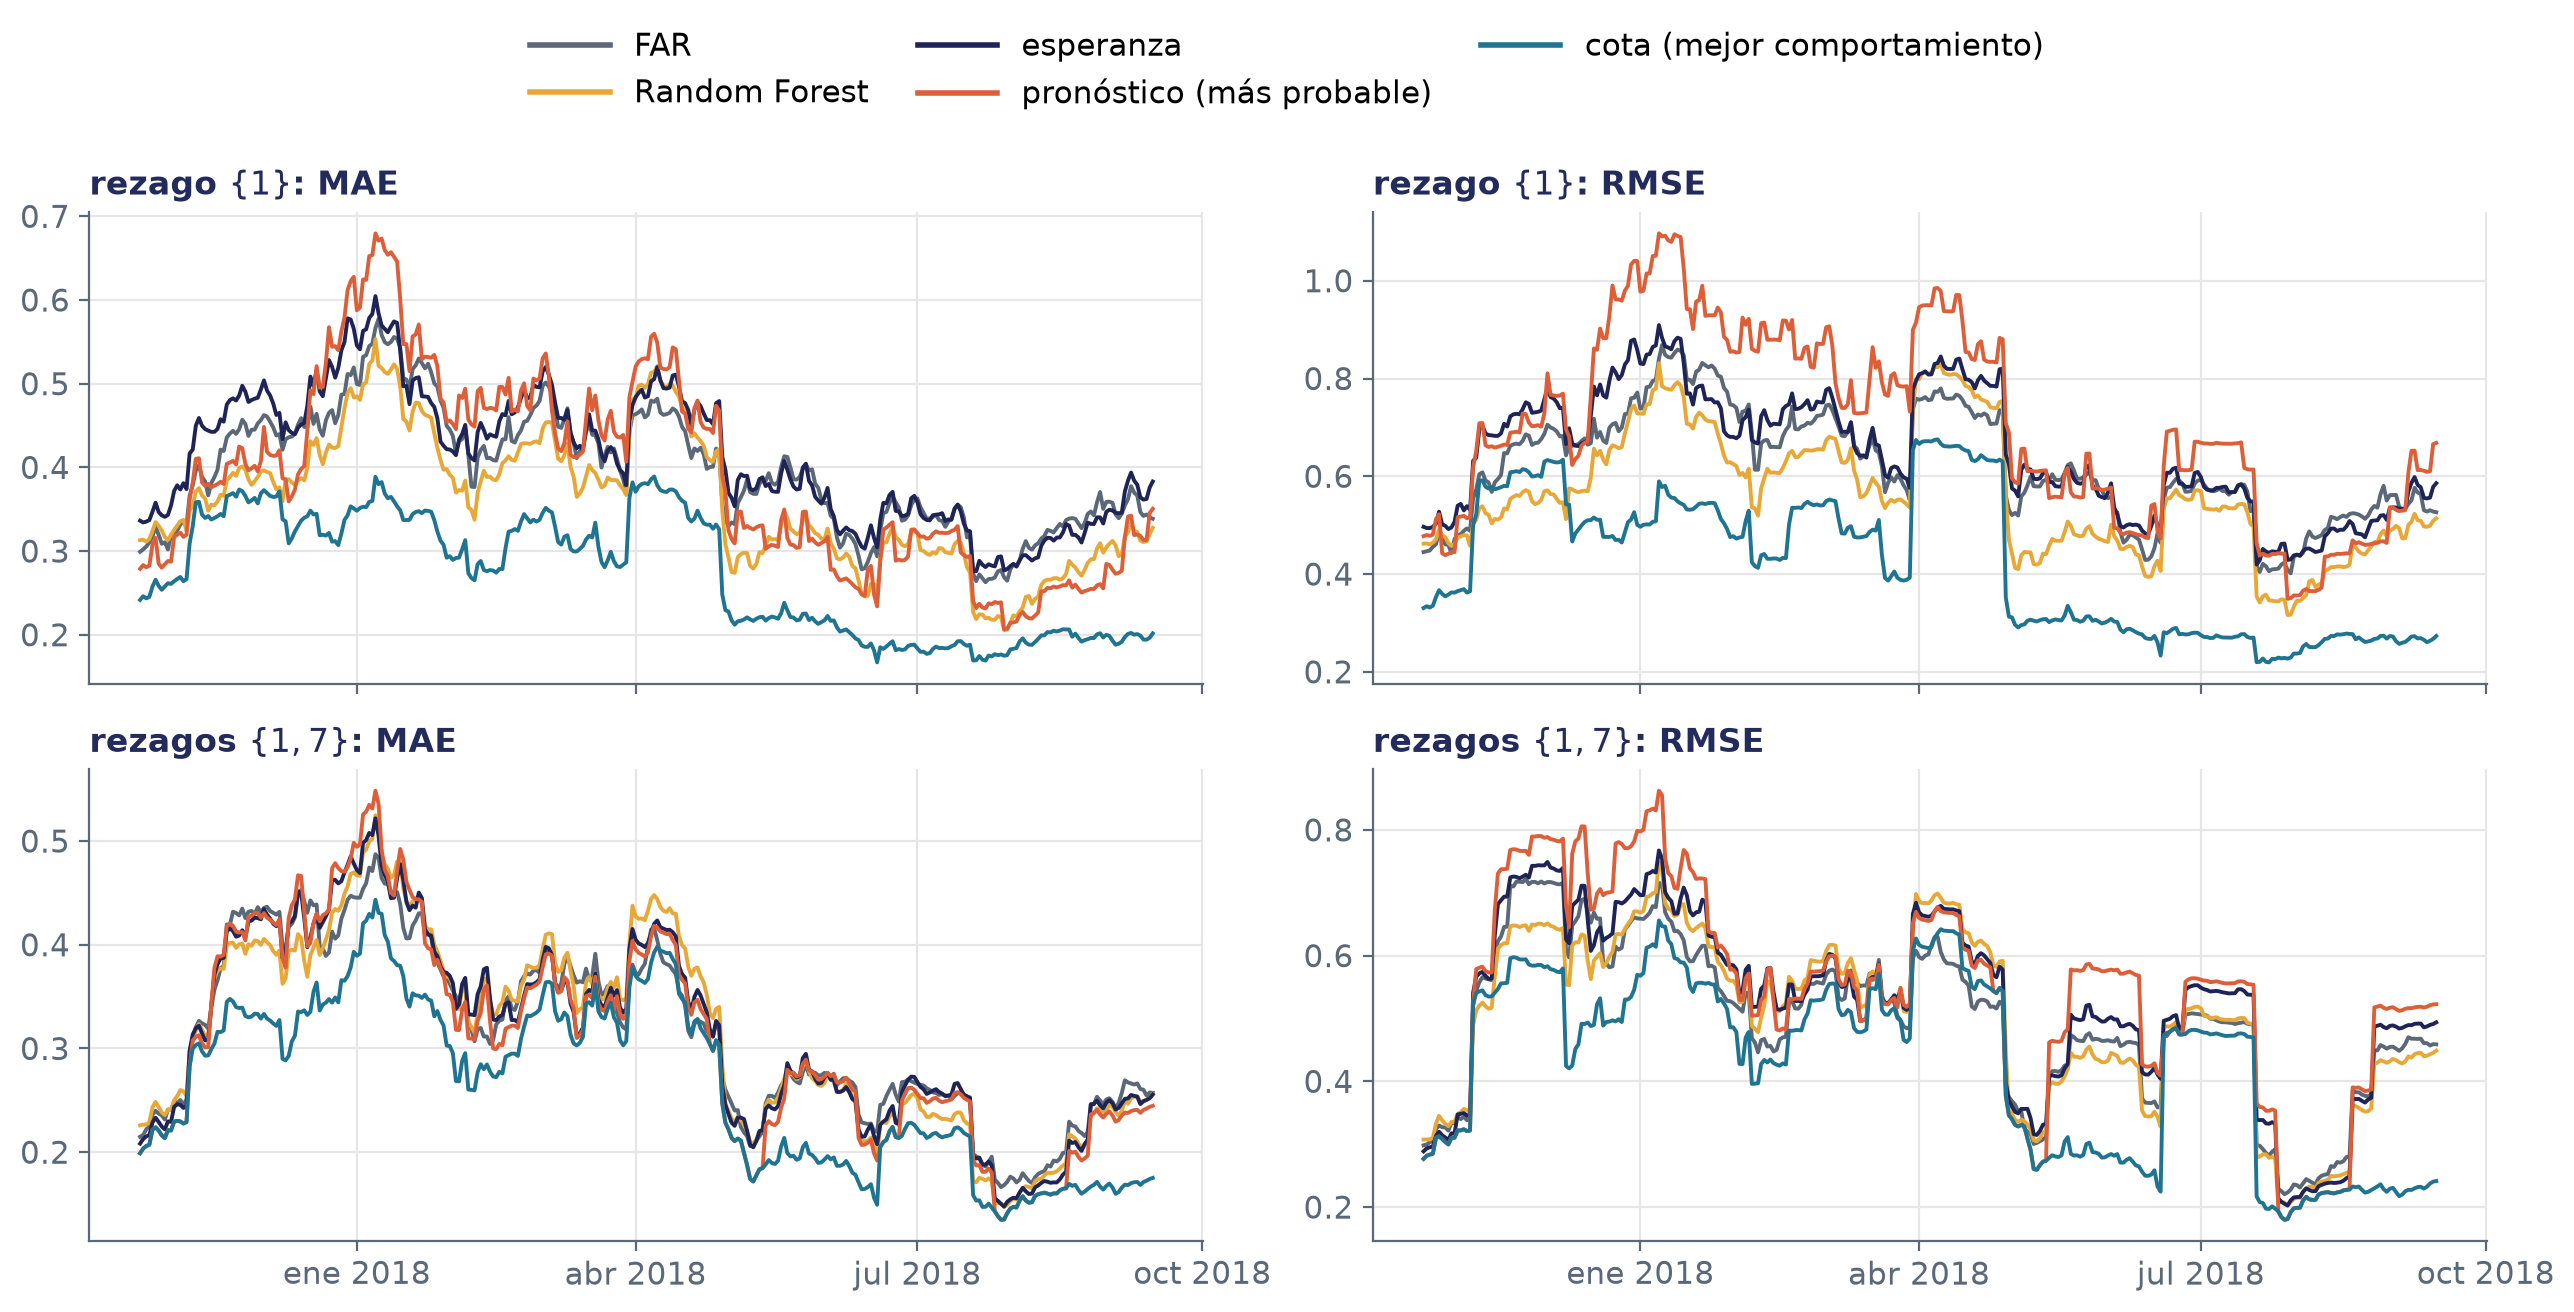
\includegraphics[width=\textwidth]{IMG/04_03/04_pronostico_ventana_w30.png}
\caption{MAE y RMSE del pronóstico por comportamiento y de la cota sobre la ventana móvil del bloque de prueba, junto a la esperanza, el FAR y el Random Forest, con rezago $\{1\}$ (arriba) y rezagos $\{1,7\}$ (abajo) ($M = 10$, $w = 30$).}
\label{fig:apl_pronostico_ventana}
\end{figure}

La Figura~\ref{fig:apl_pronostico_ventana} muestra lo mismo a lo largo del bloque de prueba. Con el rezago de un día la cota queda bajo todos los modelos en todas las ventanas, y el pronóstico se separa hacia arriba en RMSE entre diciembre y mayo, donde elegir el perfil incorrecto tiene más costo. Con ambos rezagos el pronóstico y la esperanza casi coinciden, y la cota se separa de ellos solo en algunos tramos, que son los que conservan más días con dos comportamientos.

% Fuente: 119_acierto_por_p1.csv (test, K >= 2, M = 10).
\begin{table}[H]
\centering\small
\setlength{\tabcolsep}{3.5pt}
\caption{Acierto del pronóstico por comportamiento ($K_t \ge 2$, $M = 10$) por tramo de la probabilidad del comportamiento elegido y MAE que se pierde por no elegir el mejor, en promedio sobre los orígenes del tramo.}
\label{tab:apl_acierto_p1}
\begin{tabular}{l ccc ccc}
\hline
 & \multicolumn{3}{c}{Rezago $\{1\}$} & \multicolumn{3}{c}{Rezagos $\{1,7\}$} \\
$p_{t,k^{*}}$ & Orígenes & Acierto & Pérdida & Orígenes & Acierto & Pérdida \\
\hline
$[0.5, 0.6)$ & 38 & 47\% & 0.45 & 3 & 67\% & 0.18 \\
$[0.6, 0.7)$ & 41 & 66\% & 0.24 & 9 & 78\% & 0.27 \\
$[0.7, 0.8)$ & 59 & 75\% & 0.20 & 22 & 64\% & 0.22 \\
$[0.8, 0.9)$ & 71 & 93\% & 0.04 & 52 & 88\% & 0.11 \\
$[0.9, 1]$ & 47 & 98\% & 0.01 & 42 & 98\% & 0.03 \\
\hline
\end{tabular}
\end{table}

El Cuadro~\ref{tab:apl_acierto_p1} muestra que, con el rezago de un día, el acierto sube de forma monótona con la probabilidad, de un $47\%$ entre $0.5$ y $0.6$, donde elegir equivale al azar, a un $98\%$ sobre $0.9$, y la pérdida respecto de la cota cae de $0.45$ a $0.01$. Con ambos rezagos la masa se desplaza hacia las probabilidades altas, porque la información decide el perfil. La lectura práctica es la misma que en la simulación, con una probabilidad alta se pronostica con el comportamiento más probable y con una baja se reportan las opciones y sus probabilidades.

\subsection{Selección de variables}
\label{04_03_05_seleccion}

El mecanismo de inclusión de la ecuación~\eqref{eq:gamma_prior} permite identificar qué scores rezagados afectan la ley del score que se modela. Para cada score respuesta $\xi_{tm}$ y cada covariable se reporta la probabilidad posterior de inclusión (PIP), la probabilidad de que la covariable entre en al menos uno de los átomos ocupados de la mezcla de ese score, estimada como la frecuencia de ese evento en las iteraciones retenidas. Una PIP cercana a uno indica que el rezago correspondiente interviene en la mezcla del score, y una cercana a cero, que la mezcla prescinde de él.

% Fuente: osumout y N1out de las trazas chain_fpc_<k>_iter01.mat de 101 y 102, burn = 1000; coincide con 46_pip.csv del _03.
\begin{figure}[H]
\centering
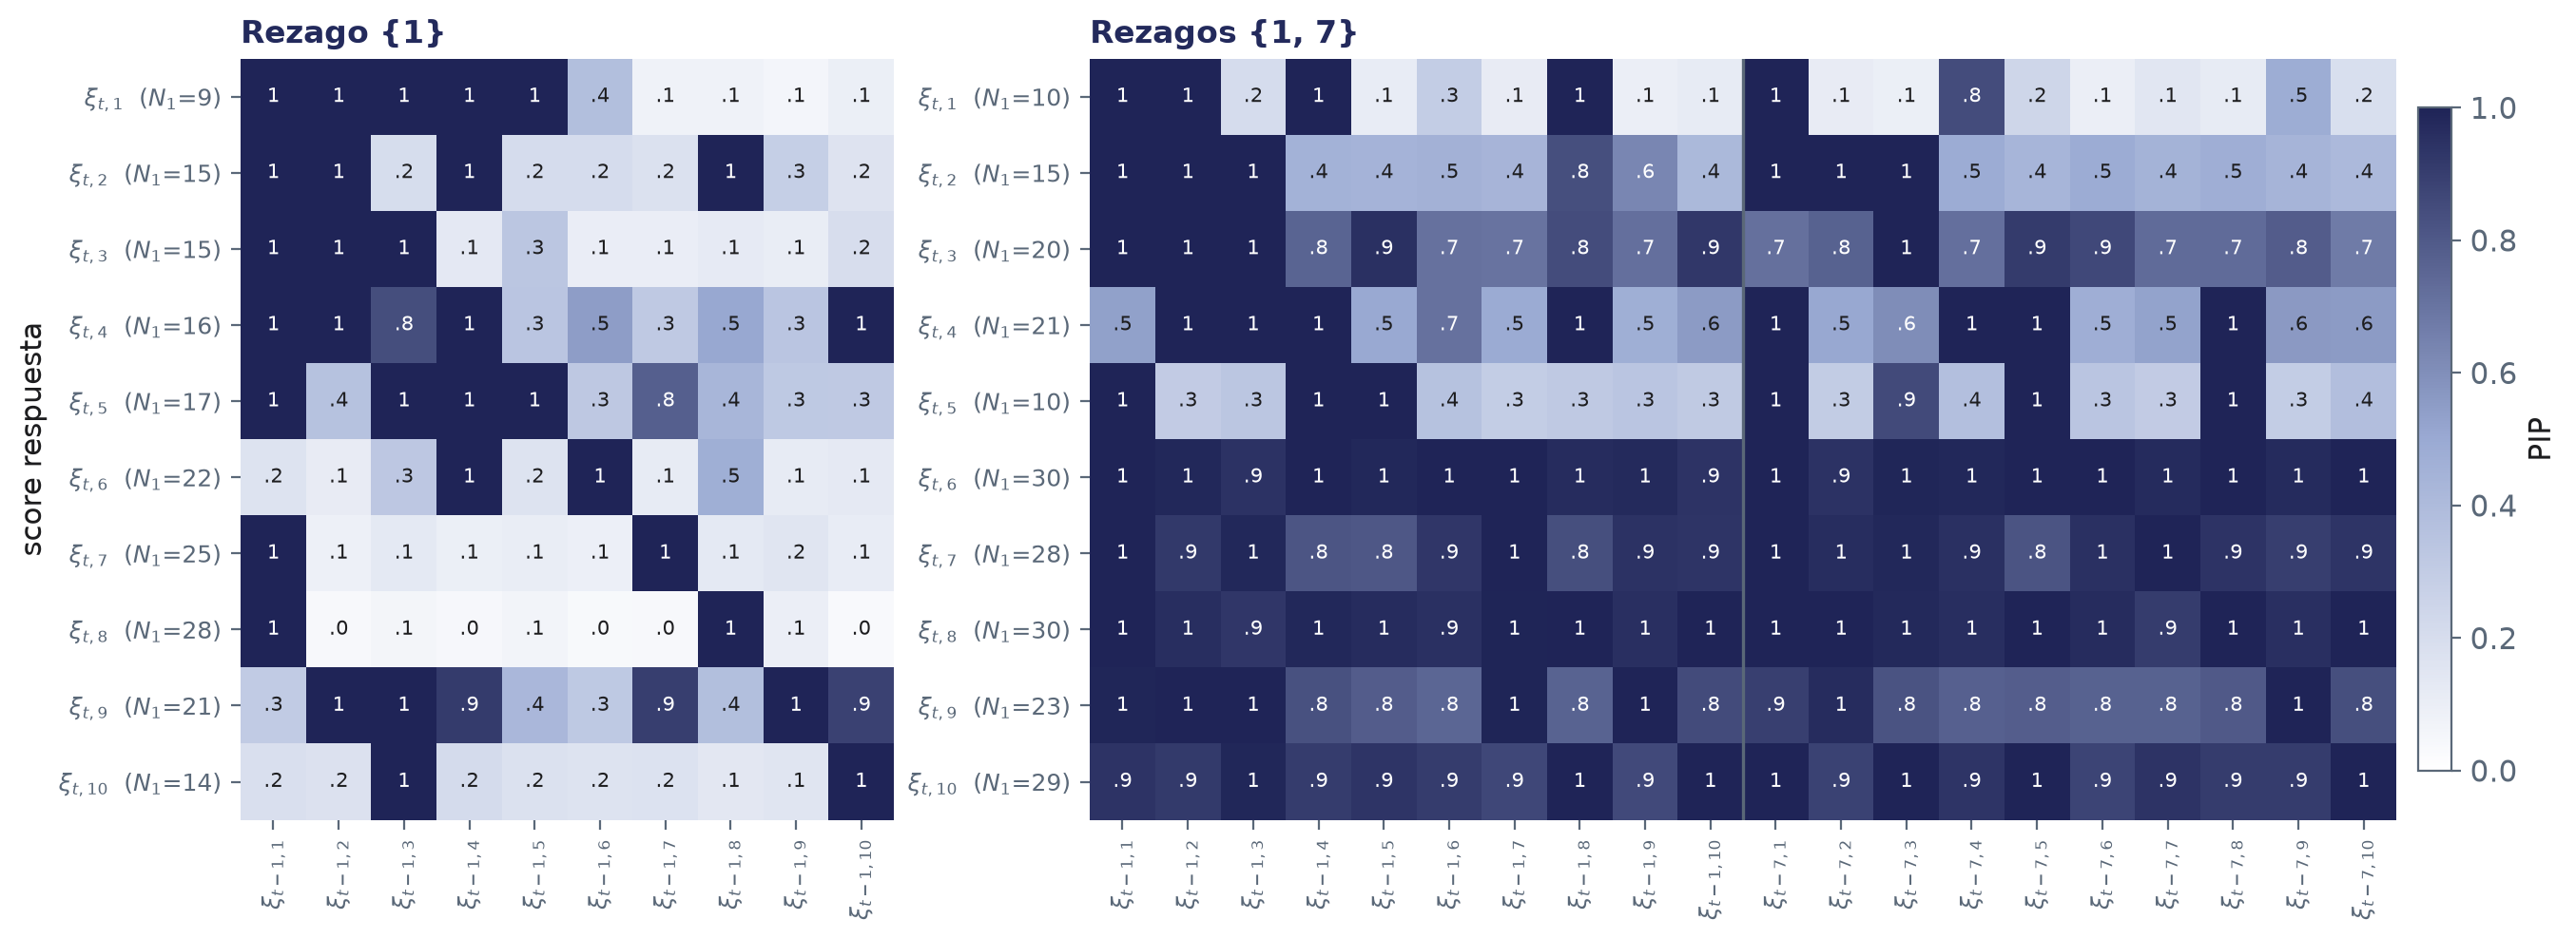
\includegraphics[width=\textwidth]{IMG/04_03/04_pip.png}
\caption{Probabilidad posterior de inclusión de cada covariable (columnas) en la mezcla de cada score (filas), con rezago $\{1\}$ (izquierda) y rezagos $\{1,7\}$ (derecha) ($M = 10$). $\xi_{t-\ell,m}$ es el score $m$ del día $t-\ell$, y $N_1$, el índice medio del último átomo ocupado de la mezcla, sobre un truncamiento de 30.}
\label{fig:apl_pip}
\end{figure}

La Figura~\ref{fig:apl_pip} muestra que, con el rezago de un día, la mezcla del primer score incluye los rezagos de los cinco primeros scores con PIP igual a uno y excluye los otros cinco, con PIP de $0.38$ o menos; la del segundo incluye los scores $1$, $2$, $4$ y $8$, y la del tercero los tres primeros. Todos los scores incluyen su propio rezago, y el rezago del primer score entra en siete de las diez mezclas.\\

Con el rezago semanal, la mezcla del primer score conserva del día anterior los scores $1$, $2$, $4$ y $8$, excluye los scores $3$ y $5$, y de la semana anterior incluye solo el primer score, con PIP igual a uno, y el cuarto, con $0.85$; los otros ocho rezagos semanales quedan en $0.48$ o menos. La mezcla del segundo score agrega los rezagos semanales de los tres primeros scores, y la del quinto los de los scores $1$, $3$, $5$ y $8$. El rezago semanal del primer score entra con PIP igual a uno en las mezclas de los scores $1$, $2$, $4$ y $5$.\\

En las mezclas que ocupan casi todo el truncamiento, la PIP no distingue entre covariables. Con el rezago semanal, las mezclas del tercer score y de los scores $6$ a $10$ ocupan entre 20 y 30 átomos, y en ellas todas las covariables tienen PIP de $0.67$ o más. Como la PIP cuenta la inclusión en cualquier átomo ocupado, es posible que con tantos átomos se acerque a uno sin que todas las covariables sean relevantes. El detalle de estas mezclas está en el Anexo~\ref{aneC_00_09_seleccion}. Con una sola cadena por especificación, además, la PIP no tiene una medida de su variabilidad entre cadenas y se lee como descriptiva.
\section{Discusión}
\label{04_04_00_discusion}

La aplicación al tráfico confirma en datos reales lo que el estudio de simulación mostraba en el escenario C-2. Cuando la ley de la curva siguiente depende de un estado que las covariables solo revelan en parte, la predictiva del PSBPM-FD reparte su masa entre comportamientos que corresponden a estados reconocibles del proceso, aquí el perfil laborable y el de fin de semana, y esa estructura se traduce en intervalos mejores que los de un modelo lineal con banda de ancho fijo, con un Winkler un $11\%$ menor que el del FAR en ambas especificaciones y menor en el $93\%$ de las ventanas con el rezago de un día y en el $76\%$ con ambos rezagos. En el error puntual la ventaja depende del resumen. Bajo MAE la mediana puntual supera al FAR en un $5.4\%$ con el rezago de un día y en un $3.7\%$ con ambos rezagos, y le gana en el $70\%$ y el $80\%$ de las ventanas, respectivamente; con ambos rezagos es además el mejor predictor en MAE y el que gana más ventanas, un $59\%$. Bajo RMSE, en cambio, la esperanza no supera al FAR, y el Random Forest es el mejor predictor puntual cuando solo se dispone del día anterior.\\

La comparación entre las dos especificaciones muestra el efecto de la información sobre los pesos de la mezcla. Al agregar el rezago semanal, la mezcla concentra la masa en un solo comportamiento en los días en que esa información decide el perfil, de martes a viernes, y conserva varios comportamientos donde no lo decide, en fines de semana, feriados y lunes. El modelo no impone la multimodalidad, más bien la produce cuando la información disponible no basta para elegir entre estados. Los comportamientos funcionan además como un agrupamiento por tipo de día, el estado latente que no entra al modelo, ya que la curva observada queda cerca del comportamiento de su tipo de día en el $96\%$ de los orígenes con dos comportamientos, y lo que la información cambia es la probabilidad que recibe cada grupo, que en los días no laborables pasa de acertar el perfil en algo más de la mitad de los casos a acertarlo en casi todos. Esa misma información mejora a todos los métodos y elimina las diferencias entre ellos en el error puntual, pero no en los intervalos, donde el PSBPM-FD mantiene su ventaja porque su ancho sigue al estado del proceso.\\

Estos resultados descansan en supuestos estructurales del modelo. La factorización de la ecuación~\eqref{eq:factorizacion} modela cada score con una mezcla univariada y supone independencia condicional entre componentes, un supuesto más razonable para los scores de la FPCA, que no están correlacionados, que para los coeficientes de una base fija, que en general lo están. Por eso el modelo trabaja sobre los scores y no directamente sobre los coeficientes, aun cuando la base sea ortonormal. Además, para que el modelo sea competitivo es necesario retener prácticamente tantos scores como coeficientes de la base, aquí $M = J = 10$, de modo que la representación conserva los detalles de la curva y no solo una versión suavizada de ella.\\

Esa misma elección condiciona la interpretación de la selección de variables. Las autofunciones de la FPCA se extienden sobre todo el dominio, de modo que un score no corresponde a un intervalo particular de $\tau$, y la PIP indica qué scores rezagados afectan a cada score sin traducirse directamente en qué horas del día anterior afectan a qué horas del día siguiente. Obtener esa interpretación requeriría una base local que conserve la estructura de cada tramo del dominio, como las B-splines, pero sus coeficientes están correlacionados, y al tratarse de mezclas univariadas y no de un modelo para el vector completo no pueden usarse directamente sin contradecir el supuesto de la factorización. La interpretabilidad de la selección y la factorización por componentes quedan así en tensión.\\

Por último, las otras cinco series del Anexo~\ref{aneD_00_00_otras_series}, sin un estado oculto que separe perfiles, tienen predictivas unimodales, y en ellas el PSBPM-FD queda cerca del FAR, lo que delimita el alcance de la ventaja que muestra el tráfico a series cuya ley condicional tiene más de un comportamiento.
\chapter{Conclusiones y Trabajo Futuro}
\label{05_00_00_conclusiones}

Esta tesis propuso el PSBPM-FD, un modelo bayesiano no paramétrico para series de tiempo funcionales que estima la distribución condicional completa de la curva siguiente dado el pasado del proceso. Las curvas se representan por sus scores de componentes principales funcionales, la ley de cada score dado el estado rezagado es una mezcla probit stick-breaking de regresiones normales, y la predictiva de los scores se transporta a la curva por la expansión funcional. Sobre esa predictiva se definieron tres predictores puntuales, tres construcciones de intervalo y los comportamientos predictivos, que identifican en cada origen los desenlaces posibles de la curva siguiente y la probabilidad de cada uno, y de ellos un pronóstico y su cota. El modelo se evaluó en tres escenarios simulados y en el tráfico de una autopista urbana, con el FAR y el Random Forest como referencias. Este capítulo reúne lo que ese estudio establece, lo que deja abierto y las direcciones en que conviene continuarlo.

\section{Conclusiones}
\label{05_01_00_conclusiones}

La primera pregunta del estudio era en qué condiciones la predicción puntual del PSBPM-FD supera a la de los modelos de referencia. La respuesta es que la ventaja sobre el FAR es grande donde la media condicional es no lineal y pequeña pero sostenida donde es lineal o casi lineal. En el escenario con cambio de régimen la esperanza reduce el error del FAR en torno a un quinto y lo supera en todas las ventanas de prueba, mientras que con heterocedasticidad condicional y con multimodalidad en la ley de los scores la reducción es de un par de puntos porcentuales que se repite en la gran mayoría de las ventanas (Cuadros~\ref{tab:res_bloqueA_ganancia} y~\ref{tab:res_bloqueA_ventanas}). En el tráfico, donde la ley de la curva siguiente es una mezcla de perfiles, la ventaja depende del resumen, ya que la mediana puntual supera al FAR bajo MAE con una y con dos covariables rezagadas y la esperanza no lo supera bajo RMSE, porque promedia perfiles que no ocurren (Sección~\ref{04_03_01_error_puntual}). Entre los predictores, la esperanza es la mejor bajo RMSE y la mediana puntual bajo MAE donde la predictiva es multimodal, como corresponde a la pérdida que cada uno minimiza, y el átomo más probable es el más débil. El Random Forest, con las mismas covariables, es el mejor predictor puntual cuando la dinámica tiene la estructura de umbral que sus cortes reproducen y cuando solo se dispone del rezago de un día en el tráfico, y queda detrás del PSBPM-FD en los demás casos.\\

La segunda pregunta era en qué condiciones los intervalos de credibilidad ofrecen un mejor desempeño, y es donde el modelo muestra su ventaja más clara. Las bandas puntuales reducen el puntaje de Winkler del FAR en los tres escenarios y en las dos especificaciones del tráfico, con una reducción de un quinto donde hay cambio de régimen y de un décimo en el tráfico, y lo superan en la mayoría de las ventanas de prueba en todos los casos (Cuadros~\ref{tab:res_bloqueB_ganancia} y~\ref{tab:apl_bloqueB_ganancia}). La razón es la misma en la simulación y en los datos reales, el ancho de la banda del PSBPM-FD sigue al estado del proceso, angosto en los tramos tranquilos y ancho en los episodios de mayor varianza, en el régimen volátil o en los días cuyo perfil la información no decide, mientras que la banda del FAR hereda una varianza residual fija y tiene el mismo ancho en todos los orígenes (Secciones~\ref{03_08_02_intervalos} y~\ref{04_03_02_intervalos}). Esa adaptación es la que una ley de innovación rígida no puede dar y la razón por la que la ventaja en los intervalos aparece incluso donde la media condicional es lineal y el error puntual empata. Entre las construcciones, la equi-colas es la referencia, la región de máxima densidad solo se separa de ella donde la predictiva tiene valles y ahí la mejora, y la banda simultánea es la única calibrada para cubrir la curva completa, al precio de un ancho que le hace perder el Winkler.\\

La tercera pregunta era en qué medida los comportamientos de la predictiva reproducen los regímenes del proceso y permiten pronosticar a partir de ellos. En el escenario con cambio de régimen los comportamientos los producen los scores que cambian de régimen y no la dimensión $M$ (Sección~\ref{03_08_03_comportamientos}), y en el tráfico corresponden a los dos tipos de día, el laborable y el no laborable, aparecen donde el calendario deja ese tipo sin decidir y la cota muestra que uno de ellos es la curva que ocurre (Secciones~\ref{04_03_03_comportamientos} y~\ref{04_03_04_pronostico}). Lo que la información cambia no es ese agrupamiento sino la probabilidad que recibe cada grupo, de modo que al agregar el rezago semanal la predictiva se vuelve unimodal en los días en que esa información decide el perfil y conserva varios comportamientos donde no lo decide. El modelo no impone la multimodalidad, la produce cuando lo que sabe no basta para elegir entre estados. Pronosticar con el comportamiento más probable es una apuesta que gana al FAR con holgura, empata con la esperanza bajo MAE y pierde bajo RMSE, porque las elecciones equivocadas pesan más que las acertadas (Cuadros~\ref{tab:res_pronostico} y~\ref{tab:apl_pronostico_101}). Su cota muestra que la predictiva contiene casi siempre la curva que ocurre, es decir, que el modelo captura la ley condicional y no solo su media, y que la pérdida del pronóstico se produce al elegir, y la probabilidad del comportamiento elegido indica cuándo conviene hacerlo, de manera que con una probabilidad alta se pronostica con el comportamiento y con una baja se reportan las opciones (Cuadros~\ref{tab:res_acierto_p1} y~\ref{tab:apl_acierto_p1}).\\

En conjunto, lo que distingue al PSBPM-FD de un modelo lineal no es el error puntual sino que su predictiva tiene la forma de la ley condicional, y esa forma es la que da los intervalos adaptativos y los comportamientos. Su alcance queda delimitado por las otras cinco series reales del Anexo~\ref{aneD_00_00_otras_series}, sin un estado oculto que separe perfiles, donde la predictiva es unimodal y el modelo queda cerca del FAR. La ventaja aparece en series cuya ley condicional tiene más de un comportamiento o cuya dispersión cambia con el estado, y es en esas series donde el modelo debe usarse.

\section{Limitaciones}
\label{05_02_00_limitaciones}

Las conclusiones anteriores descansan en un estudio de simulación con una réplica por escenario, de modo que sus cifras son descriptivas y no estiman la variabilidad entre realizaciones del generador, y el escenario con cambio de régimen está calibrado para favorecer la separación entre regímenes (Sección~\ref{03_07_02_escenarios}), por lo que la magnitud de la ventaja vale para esa configuración y no para cualquier grado de separación. En el escenario con multimodalidad en los scores, el rasgo queda en la ley conjunta y no llega a la marginal de la curva, de manera que el estudio no observa el caso en que la curva siguiente es multimodal por construcción fuera del cambio de régimen.\\

Los comportamientos reparten masa con más generosidad que la ley verdadera, y lo hacen donde el proceso cambia de régimen. En el escenario con cambio de régimen el modelo declara más de un comportamiento en el $30\%$ de los orígenes de prueba, mientras que la ley condicional es multimodal en cerca de un $9\%$ (Sección~\ref{03_08_03_comportamientos}). La diferencia se concentra en los orígenes cuyo estado se acerca al umbral, porque ahí los dos regímenes son posibles y la transición probit de los pesos, más suave que la del generador, reparte la masa entre ambos antes y después de lo que el proceso lo hace, de modo que al modelo le cuesta más decidir cuanto más cerca está el cambio. Esa masa adicional no es un régimen falso sino una opción de baja probabilidad, y su costo es pequeño, ya que las bandas y la cota no la pagan, pero sí afecta al pronóstico por comportamiento como regla de elección. Cuando la probabilidad del comportamiento elegido queda entre $0.5$ y $0.7$, elegir pierde más de lo que gana, y con los pocos orígenes de ese tramo no puede separarse si se debe a estados sobre el umbral, donde el propio proceso es incierto, o a una probabilidad optimista del modelo. Por eso la recomendación práctica es reportar las opciones y sus probabilidades en vez de elegir cuando la probabilidad es baja.\\

En la aplicación, el muestreador se ejecutó con una sola cadena por especificación, de modo que no se calcula el diagnóstico de convergencia entre cadenas y las probabilidades posteriores de inclusión se leen como descriptivas. Las mezclas de los scores menores ocupan casi todo el truncamiento de 30 átomos, y en ellas la probabilidad de inclusión no distingue entre covariables (Sección~\ref{04_03_05_seleccion}). Para que el modelo sea competitivo es necesario retener prácticamente tantos scores como funciones tiene la base, aquí $M = J = 10$, de modo que la reducción de dimensión que motiva el uso de los scores es, en la práctica, pequeña.\\

Por último, la factorización por componentes, que modela cada score con una mezcla univariada y supone independencia condicional entre ellos, es la que hace tratable la inferencia y permite ejecutar los $M$ muestreadores en paralelo, pero condiciona la interpretación. Las autofunciones se extienden sobre todo el dominio, de modo que un score no corresponde a un intervalo particular de la curva y la selección de variables indica qué scores rezagados afectan a cada score sin traducirse en qué horas del día anterior afectan a qué horas del siguiente. Una base local conservaría esa lectura, pero sus coeficientes están correlacionados y no admiten la factorización sin contradecir su supuesto. La interpretabilidad de la selección y la factorización por componentes quedan en tensión, como se discute en la Sección~\ref{04_04_00_discusion}.

\section{Trabajo Futuro}
\label{05_03_00_trabajo_futuro}

Las limitaciones anteriores señalan las direcciones en que el trabajo puede continuar. La primera es completar el estudio de simulación con un escenario en que la curva siguiente sea multimodal por construcción, con regímenes que difieran en nivel y no solo en dispersión, de modo que los comportamientos puedan contrastarse con modos verdaderos de la curva y no solo con los de la ley conjunta de los scores, y con varias réplicas por escenario, para que las diferencias entre modelos lleven una medida de su variabilidad.\\

La segunda es el modelo conjunto sobre el vector de scores. La factorización es un supuesto de conveniencia, y una mezcla única para $\boldsymbol{\xi}_t$ con átomos multivariados, cuyos pesos dependieran del mismo estado rezagado, permitiría que un mismo átomo recogiera la configuración completa de un régimen en vez de repartirla entre $M$ mezclas que solo comparten $\mathbf{z}_t$. Esa formulación eliminaría la tensión entre interpretabilidad y factorización, porque admitiría bases locales con coeficientes correlacionados, al costo de un muestreador de mayor dimensión que ya no se paraleliza por componente y de una identificación de los comportamientos que podría leerse directamente de los átomos. Una alternativa más directa, y previa a esa formulación, es ajustar el modelo tal como está sobre los coeficientes de una base local, aceptando que se viola la independencia condicional entre componentes, para ver cuánto cuesta esa violación en el desempeño predictivo. El interés está en que los scores de la FPCA, y en general los coeficientes de cualquier base ortonormalizada, no heredan la localidad de la curva, mientras que los coeficientes de una B-spline sí la tienen, cada uno gobierna un tramo del dominio; pero esa localidad se pierde en cuanto se corrige por la matriz de Gram para trabajar en la métrica de $L^2$, porque la transformación vuelve a repartir cada coeficiente sobre todo el dominio. Ajustar sobre los coeficientes crudos de la B-spline conservaría la lectura por tramos de la selección de variables, qué horas del día anterior afectan a qué horas del siguiente, y la comparación con el ajuste sobre scores diría si la independencia condicional es un supuesto que el modelo necesita o solo uno que lo hace cómodo.\\

La tercera es la calibración de las probabilidades cerca de un cambio de régimen. La transición probit de los pesos es más suave que la del proceso, de modo que al acercarse el estado al umbral la mezcla reparte la masa entre los regímenes antes y después de lo que corresponde, y eso es lo que separa al pronóstico de su cota en los orígenes de probabilidad intermedia. Una especificación de los pesos que admita transiciones más abruptas, sea con un prior menos restrictivo sobre los coeficientes de decaimiento o con un enlace distinto del probit sobre distancias, acercaría las probabilidades declaradas a las del proceso sin quitar opciones reales. Medirlo requiere más orígenes cerca del umbral que los que da una réplica, para separar la incertidumbre propia del proceso en ese tramo de la que agrega el modelo.\\

La cuarta es ampliar lo que entra al estado. La factorización admite covariables exógenas en $\mathbf{z}_t$ sin alterar su estructura, de modo que el calendario, que en el tráfico se usó solo para leer los resultados, podría entrar a los pesos de la mezcla y resolver los días que ningún rezago anuncia, y lo mismo vale para variables meteorológicas o de mercado en las otras series. Del mismo modo, el estudio se limitó a predicciones a un paso, y la extensión a horizontes mayores requiere propagar la predictiva a través de los rezagos, con comportamientos que se ramifican en cada paso.\\

Por último, el costo computacional. Con rezagos propios basta entrenar el mayor $M$ del barrido y reutilizar sus trazas para los menores, pero con los rezagos de todas las componentes cada $M$ exige un muestreador propio, y en las series reales las mezclas de los scores menores ocupan todo el truncamiento. Un truncamiento adaptativo, varias cadenas en paralelo y diagnósticos sobre cantidades invariantes a la permutación de los átomos harían más seguro el uso del modelo en series largas, que son las que más se benefician de una predictiva que cambia con el estado.

\appendix
% Los apéndices se llaman "Anexo" en el texto: lo mismo en títulos y encabezados.
\renewcommand{\appendixname}{Anexo}

\chapter{Algoritmos de Simulación}
\label{ane_00_00_anexo}
Este anexo presenta los algoritmos empleados para generar los datos del estudio de simulación del Capítulo~\ref{03_00_00_mezclas_ddp_series_tiempo_funcionales}. Cada algoritmo especifica su mecanismo generador, el rol de sus parámetros y los valores numéricos con que se emplea, los cuales se recogen en un cuadro al cierre de cada uno.\\

Todos los algoritmos especifican la dinámica directamente sobre los scores de la representación funcional. Se consideran tres algoritmos, C-1 a C-3, uno por escenario del estudio; el rasgo que cada uno introduce en la ley condicional del score, su propósito y la configuración con que se ajustan los métodos se describen en la Sección~\ref{03_07_02_escenarios}.

\section{Esquema común}
\label{ane_00_01_esquema_comun}

Esta sección presenta los elementos comunes a los tres algoritmos, la representación de las curvas en una base ortonormal, la grilla de observación, el espectro de varianzas de los scores y la generación de los scores pasivos. Los algoritmos se distinguen únicamente por el mecanismo que gobierna la dinámica de los scores activos, que se presentan a continuación.\\

Sea $\{\phi_j\}_{j=1}^{J}$ un sistema ortonormal en $L^2([0,1])$ y sea $\mu(\tau)$ la función media. Cada curva se representa como
\begin{equation}
\label{eq:ane_coef_curva}
X_t(\tau)
=
\mu(\tau)
+
\sum_{j=1}^{J}
\xi_{tj}\,\phi_j(\tau),
\end{equation}
donde $\xi_{tj}$ es el score de la $j$-ésima componente en el período $t$. Se emplea la base de Fourier sin término constante,
\begin{equation}
\label{eq:ane_fourier}
\phi_{2k-1}(\tau)=\sqrt{2}\,\sin(2\pi k\tau),
\qquad
\phi_{2k}(\tau)=\sqrt{2}\,\cos(2\pi k\tau),
\end{equation}
con $k=1,\ldots,J/2$, $J=10$, y $\mu(\tau)=\sin(2\pi\tau)$, que pertenece al espacio generado por la base.\\

La estructura temporal se especifica en el espacio de los scores y las curvas se obtienen luego mediante \eqref{eq:ane_coef_curva}. Las curvas se evalúan sobre la grilla regular $\tau_g = (g-1)/(G-1)$, $g = 1, \dots, G$, común a todos los períodos. Como la base es ortonormal y $\mu$ está en su espacio, la representación es exacta.\\

Cada algoritmo genera además un período de calentamiento de $T_{\mathrm{cal}}$ curvas que se descartan antes de retener las $T$ curvas del estudio, de modo que las condiciones iniciales no influyan en los datos.\\

La escala de los scores sigue un espectro decreciente, $\mathrm{Var}(\xi_{tj})=\lambda_j=\lambda_1 \varrho^{\,j-1}$ con $\lambda_1>0$ y $\varrho\in(0,1)$, de modo que
\begin{equation}
\label{eq:ane_escala}
\xi_{tj} = \sqrt{\lambda_j}\; \tilde{\xi}_{tj},
\end{equation}
donde $\tilde{\xi}_{tj}$ es una serie de varianza marginal unitaria cuyo mecanismo generador define cada algoritmo. Los primeros $J_a=4$ scores son los activos, por lo que llevan la dinámica distintiva del escenario. Los $J-J_a$ restantes siguen un proceso autorregresivo de primer orden común, $\tilde{\xi}_{tj}=\varphi_p\, \tilde{\xi}_{t-1,j}+\sqrt{1-\varphi_p^{2}}\,\varepsilon_{tj}$ con $\varepsilon_{tj}\overset{\mathrm{iid}}{\sim}\mathcal{N}(0,1)$, y completan el espectro sin contribuir a la estructura que el escenario busca evaluar. Las componentes se generan de forma independiente entre sí, de modo que la correlación contemporánea de los scores es nula y la descomposición de las curvas puede alinearse con $\{\phi_j\}$.\\

\begin{table}[H]
\centering
\caption{Parámetros del esquema común.}
\label{tab:ane_comun}
\begin{tabular}{llc}
\hline
Símbolo & Descripción & Valor \\
\hline
$G$          & Número de puntos de la grilla                             & $75$ \\
$T$          & Número de curvas retenidas                                & $1000$ \\
$T_{\mathrm{cal}}$        & Curvas de calentamiento                                   & $300$ \\
$J$          & Número de scores                                          & $10$ \\
$J_a$        & Número de scores activos                                  & $4$ \\
$\lambda_1$  & Varianza del primer score                                 & $0.5$ \\
$\varrho$    & Razón de decaimiento del espectro                        & $0.55$ \\
$\varphi_p$     & Coeficiente autorregresivo de los scores pasivos          & $0.3$ \\
\hline
\end{tabular}
\end{table}

\section{Algoritmos basados en Scores de la Representación Funcional}
\label{ane_00_02_algoritmos_scores}
Esta sección presenta los tres algoritmos de simulación.

\subsection{Algoritmo C-1: Heterocedasticidad condicional en los scores}
\label{ane_00_02_01_alg_c1}
Cada score activo $j\le J_a$ sigue un proceso autorregresivo con innovaciones GARCH$(1,1)$ \citep{ane_00_01_bollerslev1986generalized},
\begin{equation}\label{eq:ane_algC1_argarch}
    u_{tj} = \varphi\, u_{t-1,j} + \sigma_{tj}\, \varepsilon_{tj},
    \qquad
    \varepsilon_{tj} \overset{\mathrm{iid}}{\sim} \mathcal{N}(0,1),
\end{equation}
con varianza condicional
\begin{equation}\label{eq:ane_algC1_recursion}
    \sigma_{tj}^{2} = \Upsilon_0 + \Upsilon_1\, \sigma_{t-1,j}^{2}\,\varepsilon_{t-1,j}^{2} + \Upsilon_2\, \sigma_{t-1,j}^{2},
\end{equation}
donde $\sigma_{t-1,j}\,\varepsilon_{t-1,j}$ es la innovación del período anterior, $\Upsilon_1$ gobierna la sensibilidad de la varianza futura a esa innovación y $\Upsilon_2$ la persistencia de la varianza condicional pasada. La estacionariedad de segundo orden requiere $\Upsilon_1+\Upsilon_2<1$, y esta persistencia total fija la memoria de la volatilidad, del orden de $1/(1-\Upsilon_1-\Upsilon_2)$ períodos. El nivel base se despeja de la varianza incondicional de la innovación como $\Upsilon_0=\sigma_a^{2}(1-\Upsilon_1-\Upsilon_2)$, y $\varphi$, con $|\varphi|<1$, determina la persistencia del nivel del score.\\

El proceso $u_{tj}$ tiene varianza marginal $\sigma_a^{2}/(1-\varphi^{2})$, de modo que
\begin{equation}
\label{eq:ane_algC1_score}
\tilde{\xi}_{tj}=u_{tj}\,\frac{\sqrt{1-\varphi^{2}}}{\sigma_a},
\qquad
\xi_{tj}=\sqrt{\lambda_j}\,\tilde{\xi}_{tj},
\end{equation}
tiene varianza $\lambda_j$ para todo $j$, conforme a \eqref{eq:ane_escala}.\\

La generación procede en los pasos que siguen.
\begin{enumerate}
    \item Se fijan $\varphi$, $\Upsilon_1$, $\Upsilon_2$ y $\sigma_a^{2}$, y se calcula $\Upsilon_0$.

    \item Para cada score activo se inicializan $\sigma_{1j}^{2}=\sigma_a^{2}$ y $u_{0j}=0$, y se itera \eqref{eq:ane_algC1_argarch}--\eqref{eq:ane_algC1_recursion} durante $T_{\mathrm{cal}}+T$ períodos.

    \item Los scores pasivos se generan como se indica en el esquema común.

    \item Se descartan los $T_{\mathrm{cal}}$ primeros períodos, se obtienen los scores mediante \eqref{eq:ane_algC1_score} y se reconstruyen las curvas mediante \eqref{eq:ane_coef_curva}.
\end{enumerate}

\begin{table}[H]
\centering
\caption{Parámetros del Algoritmo~C-1.}
\label{tab:ane_algC1}
\begin{tabular}{llc}
\hline
Símbolo & Descripción & Valor \\
\hline
$\varphi$       & Coeficiente autorregresivo                          & $0.5$ \\
$\Upsilon_1$    & Sensibilidad a la innovación reciente               & $0.25$ \\
$\Upsilon_2$    & Persistencia de la varianza condicional pasada      & $0.60$ \\
$\sigma_a^{2}$  & Varianza incondicional de la innovación             & $1.0$ \\
\hline
\end{tabular}
\end{table}

\subsection{Algoritmo C-2: Cambio de régimen por umbral en los scores}
\label{ane_00_02_02_alg_c2}
Cada score activo $j\le J_a$ evoluciona en una coordenada cruda $u_{tj}$ con dos regímenes, $A$ y $B$, asignados mediante un umbral $u_j^{\star}$ sobre $u_{t-1,j}$. Condicionalmente al régimen $I_{tj}=k\in\{A,B\}$,
\begin{equation}\label{eq:ane_algC2}
    u_{tj}=\mu_{kj}+\varphi_{kj}\,u_{t-1,j}+\sigma_{kj}\,\varepsilon_{tj},
    \qquad
    \varepsilon_{tj}\overset{\mathrm{iid}}{\sim}\mathcal{N}(0,1),
\end{equation}
de modo que los regímenes difieren en nivel $\mu_{kj}$, persistencia $\varphi_{kj}$ y escala $\sigma_{kj}$, donde el régimen $A$ es persistente y de escala pequeña, y el $B$ revierte y es más volátil.\\

La asignación es un probit sobre el rezago propio. Con $\Phi$ la función de distribución normal estándar y $\varsigma_j>0$ el ancho de la transición,
\begin{align}
    \Pr(I_{tj}=B\mid u_{t-1,j}) &= \Phi\!\left(\frac{u_{t-1,j}-u_j^{\star}}{\varsigma_j}\right), \label{eq:ane_algC2_probs}\\
    \Pr(I_{tj}=A\mid u_{t-1,j}) &= 1-\Pr(I_{tj}=B\mid u_{t-1,j}). \nonumber
\end{align}
Con $\varsigma_j\to0$ la asignación se vuelve determinista y el escenario es un SETAR clásico, mientras que un $\varsigma_j$ positivo hace la transición suave.\\

La media condicional es exacta,
\begin{align}
    \mathbb{E}\bigl[u_{tj}\mid u_{t-1,j}\bigr]
    &=\Pr(I_{tj}=A\mid u_{t-1,j})\bigl(\mu_{Aj}+\varphi_{Aj}\,u_{t-1,j}\bigr) \nonumber\\
    &\quad+\Pr(I_{tj}=B\mid u_{t-1,j})\bigl(\mu_{Bj}+\varphi_{Bj}\,u_{t-1,j}\bigr), \label{eq:ane_algC2_oraculo}
\end{align}
y se registra en cada período junto con el régimen sorteado. El generador usa un único rezago, aunque los métodos reciben $q = 4$, como indica el Cuadro~\ref{tab:dis_escenarios}.\\

El score se obtiene estandarizando $u_{tj}$ con sus momentos poblacionales $(\mu_j^{u},\sigma_j^{u})$, estimados una sola vez mediante una simulación larga, y escalando por \eqref{eq:ane_escala},
\begin{equation}
\label{eq:ane_algC2_score}
\tilde{\xi}_{tj}=\frac{u_{tj}-\mu_j^{u}}{\sigma_j^{u}},
\qquad
\xi_{tj}=\sqrt{\lambda_j}\,\tilde{\xi}_{tj}.
\end{equation}
La estandarización pertenece al generador, que fija la escala del escenario, y no se aplica a los datos que recibe un método.\\

La generación procede en los pasos que siguen.
\begin{enumerate}
    \item Se fijan, para cada score activo, el umbral $u_j^{\star}$, el ancho $\varsigma_j$ y los parámetros $(\mu_{kj},\varphi_{kj},\sigma_{kj})$ de los dos regímenes.

    \item Para cada período se calcula la probabilidad \eqref{eq:ane_algC2_probs} a partir de $u_{t-1,j}$ y se sortea $I_{tj}$. La secuencia de regímenes no se entrega a los métodos.

    \item Se genera $u_{tj}$ mediante \eqref{eq:ane_algC2}, con el régimen sorteado.

    \item Los scores pasivos se generan como se indica en el esquema común.

    \item Se descartan los $T_{\mathrm{cal}}$ primeros períodos, se obtienen los scores mediante \eqref{eq:ane_algC2_score} y se reconstruyen las curvas mediante \eqref{eq:ane_coef_curva}.
\end{enumerate}

\begin{table}[H]
\centering
\caption{Parámetros del Algoritmo~C-2.}
\label{tab:ane_algC2}
\begin{tabular}{l p{0.48\textwidth} c}
\hline
Símbolo & Descripción & Valor \\
\hline
$K$                       & Número de regímenes                                    & $2$ \\
$u_j^{\star}$             & Umbral sobre el rezago propio                          & $0$ \\
$\varsigma_j$                     & Ancho de la transición probit                          & Cuadro~\ref{tab:ane_algC2_scores} \\
$\mu_{kj},\ \varphi_{kj},\ \sigma_{kj}$ & Nivel, coeficiente autorregresivo y escala del régimen $k$ & Cuadro~\ref{tab:ane_algC2_scores} \\
$(\mu_j^{u},\sigma_j^{u})$               & Media y desviación poblacionales de $u_{tj}$           & Simulación larga \\
\hline
\end{tabular}
\end{table}

\begin{table}[H]
\centering
\caption{Parámetros del Algoritmo~C-2 por score activo.}
\label{tab:ane_algC2_scores}
\small\setlength{\tabcolsep}{5pt}
\begin{tabular}{lcccccccc}
\hline
$j$ & $\varsigma_j$ & $\mu_{Aj}$ & $\varphi_{Aj}$ & $\sigma_{Aj}$ & $\mu_{Bj}$ & $\varphi_{Bj}$ & $\sigma_{Bj}$ & $u_j^{\star}$ \\
\hline
$1$ & $0.10$ & $0$ & $0.8$ & $0.25$ & $2.5$ & $-0.9$ & $1.0$ & $0$ \\
$2$ & $0.10$ & $0$ & $0.6$ & $0.25$ & $2.0$ & $-0.9$ & $1.0$ & $0$ \\
$3$ & $0.25$ & $0$ & $0.8$ & $0.40$ & $2.0$ & $-0.9$ & $1.0$ & $0$ \\
$4$ & $0.25$ & $0$ & $0.6$ & $0.40$ & $2.5$ & $-0.9$ & $1.0$ & $0$ \\
\hline
\end{tabular}
\end{table}

\subsection{Algoritmo C-3: Multimodalidad en los scores}
\label{ane_00_02_03_alg_c3}
Este algoritmo genera el vector de scores con una mezcla de $K$ mecanismos lineales, cuya selección depende de la historia reciente del proceso.\\

Sea $I_t\in\{1,\ldots,K\}$ la variable latente que identifica el mecanismo utilizado en el período $t$. Condicionalmente a $I_t=k$, el vector de scores se genera mediante
\begin{equation}
\label{eq:ane_algC3}
\boldsymbol{\xi}_t
=
\boldsymbol{\mu}_{I_t}
+
\sum_{\ell=1}^{q}
A_{I_t,\ell}\,
\boldsymbol{\xi}_{t-\ell}
+
\boldsymbol{\varepsilon}_t,
\end{equation}
donde $\boldsymbol{\xi}_t=(\xi_{t1},\ldots,\xi_{tJ})^\top$ es el vector de scores, $\boldsymbol{\mu}_{I_t}$ es la localización del mecanismo seleccionado, $A_{I_t,\ell}$ es la matriz de dependencia asociada al $\ell$-ésimo rezago y $\boldsymbol{\varepsilon}_t$ es un vector de innovaciones gaussianas independientes de $I_t$. Los mecanismos comparten el patrón de dependencia de las matrices $A_{k,\ell}$ y difieren en sus valores.\\

La selección del mecanismo depende de los scores correspondientes a múltiples rezagos mediante
\begin{equation}
\label{eq:ane_algC3_asignacion}
\Pr
\left(
I_t=k
\mid
\boldsymbol{\xi}_{t-1},
\ldots,
\boldsymbol{\xi}_{t-q}
\right)
=
\frac{
\exp\bigl\{
\eta_k
\left(
\boldsymbol{\xi}_{t-1},
\ldots,
\boldsymbol{\xi}_{t-q}
\right)
\bigr\}
}{
\displaystyle
\sum_{k'=1}^{K}
\exp\bigl\{
\eta_{k'}
\left(
\boldsymbol{\xi}_{t-1},
\ldots,
\boldsymbol{\xi}_{t-q}
\right)
\bigr\}
},
\end{equation}
donde $\eta_k(\cdot)$ es afín en los scores considerados y el mecanismo 1 es la referencia del softmax, $\eta_1\equiv 0$.\\

Para incorporar dependencia temporal de más de un período se emplean $q=2$ rezagos, de modo que tanto la selección del mecanismo como la generación de los scores utilizan $\boldsymbol{\xi}_{t-1}$ y $\boldsymbol{\xi}_{t-2}$. La dinámica distintiva se concentra en los $J_a$ scores activos; los scores restantes siguen el proceso autorregresivo del esquema común, de modo que el espectro de varianzas sea el de \eqref{eq:ane_escala}.\\

Los valores se especifican en la coordenada estandarizada $\tilde{\xi}_{tj}=\xi_{tj}/\sqrt{\lambda_j}$ de \eqref{eq:ane_escala}, de modo que un coeficiente cruzado se lee igual cualquiera sea la varianza de las componentes que conecta. En la escala de los scores, con $\boldsymbol{\Lambda}^{1/2}=\mathrm{diag}(\sqrt{\lambda_1},\ldots,\sqrt{\lambda_J})$, $\boldsymbol{\mu}_k=\boldsymbol{\Lambda}^{1/2}\tilde{\boldsymbol{\mu}}_k$, $A_{k,\ell}=\boldsymbol{\Lambda}^{1/2}\tilde{A}_{k,\ell}\boldsymbol{\Lambda}^{-1/2}$, $\eta_k(\boldsymbol{\xi})=\tilde{\eta}_k(\boldsymbol{\Lambda}^{-1/2}\boldsymbol{\xi})$ y $\mathrm{Var}(\varepsilon_{tj})=\lambda_j\tilde\sigma_j^{2}$. Los tres mecanismos son un centro ($k=1$) y dos niveles, alto ($k=2$) y bajo ($k=3$), que se separan solo en la localización del primer score, $\tilde\mu_{k1}=0,\,+1,\,-1$, con $\tilde\mu_{kj}=0$ para $j\ge2$. La asignación es
\begin{align}
\tilde{\eta}_1 &= 0, \nonumber\\
\tilde{\eta}_2 &= -2.1 + 1.75\,\tilde{\xi}_{t-1,1} + 0.7\,\tilde{\xi}_{t-2,1} + 0.5\,\tilde{\xi}_{t-1,2}, \label{eq:ane_algC3_q}\\
\tilde{\eta}_3 &= -2.1 - 1.75\,\tilde{\xi}_{t-1,1} - 0.7\,\tilde{\xi}_{t-2,1} + 0.5\,\tilde{\xi}_{t-1,2}. \nonumber
\end{align}
Las matrices $\tilde A_{k,\ell}$ comparten el patrón del Cuadro~\ref{tab:ane_algC3_mecanismos}, la diagonal del bloque activo en el primer rezago y cuatro entradas cruzadas, y difieren en los valores; las entradas no listadas son cero. La entrada $(j,m)$ de $\tilde A_{k,\ell}$ es el coeficiente con que el score $m$ rezagado $\ell$ períodos entra en el score $j$. Los scores pasivos conservan su coeficiente $\varphi_p$ en el primer rezago, igual en los tres mecanismos. La innovación tiene desviación $\tilde\sigma_j$ en el bloque activo y $\sqrt{1-\varphi_p^{2}}$ en el pasivo.\\

La generación procede en los pasos que siguen.
\begin{enumerate}
    \item Se fijan el número de mecanismos $K$, los vectores $\boldsymbol{\mu}_k$, las matrices $A_{k,\ell}$ y las funciones de asignación $\eta_k(\cdot)$.

    \item Se calculan las probabilidades condicionales de los mecanismos mediante \eqref{eq:ane_algC3_asignacion}, utilizando los scores de los dos rezagos anteriores.

    \item Se sortea $I_t$ a partir de dichas probabilidades. La secuencia de mecanismos no se entrega a los métodos.

    \item Se genera $\boldsymbol{\xi}_t$ mediante \eqref{eq:ane_algC3}, con los parámetros del mecanismo seleccionado.

    \item Se descartan los $T_{\mathrm{cal}}$ primeros períodos y se reconstruyen las curvas mediante \eqref{eq:ane_coef_curva}.
\end{enumerate}

\begin{table}[H]
\centering
\caption{Parámetros del Algoritmo~C-3 (coordenada estandarizada $\tilde{\xi}$).}
\label{tab:ane_algC3}
\begin{tabular}{llc}
\hline
Símbolo & Descripción & Valor \\
\hline
$K$                  & Número de mecanismos                                   & $3$ \\
$q$                  & Número de rezagos utilizados                           & $2$ \\
$\tilde\mu_{k1}$     & Localización del primer score, $k=1,2,3$               & $0,\ +1,\ -1$ \\
$\tilde{\eta}_k$         & Funciones de asignación                                & \eqref{eq:ane_algC3_q} \\
$\tilde A_{k,\ell}$  & Matrices de dependencia                                & Cuadro~\ref{tab:ane_algC3_mecanismos} \\
$\tilde\sigma_j$     & Desviación de la innovación, $j=1,\ldots,4$            & $0.45,\ 0.75,\ 0.80,\ 0.80$ \\
\hline
\end{tabular}
\end{table}

\begin{table}[H]
\centering
\caption{Entradas no nulas de $\tilde A_{k,\ell}$ en el bloque activo, por mecanismo.}
\label{tab:ane_algC3_mecanismos}
\small\setlength{\tabcolsep}{4pt}
\begin{tabular}{clrrrrrrrr}
\hline
 & & \multicolumn{6}{c}{$\ell=1$} & \multicolumn{2}{c}{$\ell=2$} \\
$k$ & Mecanismo & $(1,1)$ & $(2,2)$ & $(3,3)$ & $(4,4)$ & $(2,1)$ & $(3,2)$ & $(1,1)$ & $(4,3)$ \\
\hline
$1$ & Centro      & $0.2$ & $0.3$ & $0.3$ & $0.3$ & $0.2$  & $0.8$  & $-0.1$ & $-0.6$ \\
$2$ & Nivel alto  & $0.2$ & $0.4$ & $0.2$ & $0.2$ & $0.5$  & $-0.3$ & $0.1$  & $0.3$ \\
$3$ & Nivel bajo  & $0.2$ & $0.4$ & $0.2$ & $0.2$ & $-0.5$ & $-0.3$ & $0.1$  & $0.3$ \\
\hline
\end{tabular}
\end{table}

\section{Configuración del estudio de simulación}
\label{ane_00_03_configuracion}
Esta sección recoge la configuración con que se corrió el estudio de simulación de la Sección~\ref{03_07_00_diseno_estudio_simulacion}, es decir, partición y ventana móvil, muestreador y predictiva, modelos de referencia, métricas por resumen y constantes de los comportamientos.\\


El Cuadro~\ref{tab:dis_particion} presenta la partición temporal, la ventana móvil y las referencias de los cuadros del capítulo; las ventanas que cruzan $T_0$ se excluyen de todo agregado.

\begin{table}[H]
\centering\small
\caption{Partición temporal, ventana móvil y referencias de los cuadros.}
\label{tab:dis_particion}
\begin{tabular}{p{0.14\textwidth} p{0.56\textwidth} p{0.18\textwidth}}
\hline
Símbolo & Descripción & Valor \\
\hline
$T_0$              & Corte entrenamiento / prueba ($70\%$ de las $T = 1000$ curvas del Cuadro~\ref{tab:ane_comun}) & $700$ \\
Horizonte          & Pasos adelante de la predicción                 & $1$ \\
$w$                & Anchos de la ventana móvil                      & $\{20, 30, 40\}$ \\
$w_{\mathrm{ref}}$ & Ancho reportado en el capítulo                  & $30$ \\
Paso               & Desplazamiento entre ventanas                   & $1$ \\
$M_{\mathrm{ref}}$ & Dimensión del estado en los cuadros, la mayor del barrido de cada escenario (Cuadro~\ref{tab:dis_escenarios}) & $10$ ($6$ en C-3) \\
$1-\zeta$          & Nivel de los intervalos de credibilidad         & $0.95$ \\
\hline
\end{tabular}
\end{table}

El Cuadro~\ref{tab:dis_mcmc} recoge la configuración del muestreador (Sección~\ref{03_04_00_modelo_propuesto_psbpm_fd}) y de la predictiva; con $a_\nu = 0.5$ la varianza predictiva no existe (Sección~\ref{03_05_05_intervalos_predictivos}) y no se reporta.

\begin{table}[H]
\centering\small
\caption{Configuración del muestreador y de la predictiva.}
\label{tab:dis_mcmc}
\begin{tabular}{p{0.16\textwidth} p{0.50\textwidth} p{0.22\textwidth}}
\hline
Símbolo & Descripción & Valor \\
\hline
$N$                   & Truncamiento del stick-breaking                         & $30$ \\
$L_j$                 & Puntos de la grilla de localización por predictor       & $50$ \\
Iteraciones           & Por cadena / descartadas                                & $2500$ / $500$ \\
Cadenas               & Cadenas independientes por score                        & $3$ \\
$a_\nu, a_\varkappa, b_\varkappa$ & Forma de las precisiones y de la contracción  & $0.5$ \\
$b_\nu$               & Escala de la precisión del átomo                        & $0.5\,\mathrm{sd}_m^{2}$ \\
$\nu_{\rho_j}$        & Precisión a priori de los coeficientes de decaimiento $\rho_{hj}$ & $10\,\mathrm{sd}_j^{2}$ \\
$(a_{\varpi_j}, b_{\varpi_j})$ & Inclusión, rezago propio de orden uno / resto      & $(0.5, 0.5)$ / $(0.5, 5)$ \\
$S$                   & Extracciones de la predictiva por origen                & $1000$ \\
\hline
\end{tabular}
\end{table}

Los modelos de referencia siguen el Cuadro~\ref{tab:dis_referencia}. El FAR se estima sobre los coeficientes completos de la representación, en la métrica $L^2$, con orden fijo igual al número de rezagos del escenario, para no darle una ventaja de especificación que el PSBPM-FD no tiene; su intervalo es gaussiano con los residuos de entrenamiento. El Random Forest comparte la especificación del PSBPM-FD, un modelo por score con las mismas covariables, de modo que la diferencia entre ambos es solo el mecanismo que liga covariables y respuesta.

\begin{table}[H]
\centering\small
\caption{Ajuste de los modelos de referencia.}
\label{tab:dis_referencia}
\begin{tabular}{p{0.16\textwidth} p{0.36\textwidth} p{0.38\textwidth}}
\hline
Modelo & Elemento & Valor \\
\hline
FAR($p$) & Orden $p$                       & Número de rezagos del escenario, fijo \\
         & Dimensión del subespacio       & Por predicción a un paso, tope $J$ \\
         & Tramo de selección              & Último $20\%$ del entrenamiento \\
         & Intervalo                       & Gaussiano, residuos de entrenamiento, $\sigma(\tau)$ \\
Random Forest & Árboles / hojas mínimas / covariables por corte & $500$ / $5$ / $\sqrt{d}$ \\
         & Orden de rezago                 & Por error absoluto en ventanas de entrenamiento \\
\hline
\end{tabular}
\end{table}

El Cuadro~\ref{tab:dis_resumen_metrica} indica, para cada métrica, sobre qué resumen de la predictiva del PSBPM-FD se calcula y contra qué modelos se compara; el Random Forest no entrega intervalos.

\begin{table}[H]
\centering\small
\caption{Métricas reportadas, resumen del PSBPM-FD sobre el que se calculan y modelos comparados.}
\label{tab:dis_resumen_metrica}
\begin{tabular}{p{0.30\textwidth} p{0.38\textwidth} p{0.22\textwidth}}
\hline
Métrica (Sección~\ref{02_02_03_criterios_evaluacion}) & Resumen del PSBPM-FD & Modelos comparados \\
\hline
RMSE, MAE & Esperanza, mediana puntual, átomo más probable & FAR, Random Forest \\
RMSE, MAE (solo C-2) & Pronóstico por comportamiento (Sección~\ref{03_06_03_descripcion}) y mejor comportamiento (cota) & FAR, Random Forest, por separado \\
$\overline{\mathrm{E}}_{\max}$, $\mathrm{E}_{\max}^{\mathrm{glob}}$ (anexo) & Esperanza en los cuadros; los tres predictores en las figuras & FAR, Random Forest \\
Winkler, MPIW, PICP & Intervalo equi-colas, banda simultánea, región de máxima densidad & FAR \\
$\overline{\mathrm{W}}_{\max}$, $\mathrm{W}_{\max}^{\mathrm{glob}}$, PICPB (anexo) & Los mismos intervalos & FAR \\
\hline
\end{tabular}
\end{table}

El Cuadro~\ref{tab:dis_comportamientos} fija las constantes del análisis de comportamientos, que se evalúan solo en C-2. La ventana de detalle de $N_{\mathrm{det}}$ orígenes consecutivos de prueba es la de más cambios de régimen verdadero, calculado sobre lo que el generador registra y nunca sobre lo predicho. El pronóstico por comportamiento y su cota se comparan con la esperanza, el FAR y el Random Forest, sobre todos los orígenes de prueba y sobre los de $K_t \geq 2$, y el acierto de la elección se lee por tramos de $p_{t,k^{*}}$.

\begin{table}[H]
\centering\small
\caption{Constantes del análisis de comportamientos.}
\label{tab:dis_comportamientos}
\begin{tabular}{p{0.20\textwidth} p{0.46\textwidth} p{0.22\textwidth}}
\hline
Elemento & Descripción & Valor \\
\hline
$S$               & Extracciones del vector de scores por origen       & $1000$ \\
Inicios           & Inicios aleatorios de $k$-medias                   & $10$ \\
Cociente de valle & Umbral de \eqref{eq:valle} para declarar dos modos & $0.5$ \\
Núcleo            & Estimador de densidad sobre la proyección          & Gaussiano, ancho de Scott \\
$\zeta$           & Masa mínima de un comportamiento                   & $0.05$ \\
Recorte           & Cuantiles de recorte cuando $a_\nu \leq 1$         & $0.5\%$ y $99.5\%$ \\
$N_{\mathrm{det}}$ & Orígenes de la ventana de detalle                 & $10$ \\
\hline
\end{tabular}
\end{table}

\chapter{Resultados Complementarios del Estudio de Simulación}
\label{aneB_00_00_resultados_simulacion}

Este anexo reúne los resultados del estudio de simulación que no se reportan en el cuerpo del Capítulo~\ref{03_00_00_mezclas_ddp_series_tiempo_funcionales}. Las figuras por origen y por componente corresponden a $M_{\mathrm{ref}} = 10$ en C-1 y C-2 y a $M_{\mathrm{ref}} = 6$ en C-3.

\section{Métricas completas por número de componentes}
\label{aneB_00_01_metricas_por_M}

Las diez métricas del Marco Teórico en el bloque de prueba para cada $M$ del barrido, como promedio sobre las ventanas de ancho $w = 30$, a saber, las cuatro métricas de error para la esperanza del PSBPM-FD, el FAR y el Random Forest, y las seis métricas de intervalo para las tres construcciones de intervalo del PSBPM-FD y para el FAR.

\subsection{Escenario C-1 (GARCH)}
\label{aneB_00_01_02_metricas_garch}

\begin{table}[H]
\centering\footnotesize
\setlength{\tabcolsep}{3pt}
\caption{C-1 (GARCH). Métricas de error en el bloque de prueba por $M$ (promedio sobre las ventanas, $w = 30$).}
\label{tab:aneB_A_C1}
\resizebox{\textwidth}{!}{%
\begin{tabular}{c cccc cccc cccc}
\hline
 & \multicolumn{4}{c}{PSBPM-FD (esperanza)} & \multicolumn{4}{c}{FAR} & \multicolumn{4}{c}{Random Forest} \\
$M$ & MAE & RMSE & $\overline{\mathrm{E}}_{\max}$ & $\mathrm{E}_{\max}^{\mathrm{glob}}$ & MAE & RMSE & $\overline{\mathrm{E}}_{\max}$ & $\mathrm{E}_{\max}^{\mathrm{glob}}$ & MAE & RMSE & $\overline{\mathrm{E}}_{\max}$ & $\mathrm{E}_{\max}^{\mathrm{glob}}$ \\
\hline
$1$ & 0.754 & 0.951 & 1.673 & 3.141 & 0.723 & 0.906 & 1.615 & 2.942 & 0.764 & 0.967 & 1.685 & 3.268 \\
$2$ & 0.739 & 0.923 & 1.644 & 2.949 & 0.723 & 0.906 & 1.615 & 2.942 & 0.753 & 0.943 & 1.668 & 3.111 \\
$3$ & 0.724 & 0.903 & 1.609 & 2.914 & 0.723 & 0.906 & 1.615 & 2.942 & 0.740 & 0.927 & 1.632 & 3.013 \\
$4$ & 0.716 & 0.895 & 1.600 & 2.919 & 0.723 & 0.906 & 1.615 & 2.942 & 0.734 & 0.922 & 1.627 & 3.049 \\
$5$ & 0.714 & 0.893 & 1.592 & 2.893 & 0.723 & 0.906 & 1.615 & 2.942 & 0.733 & 0.921 & 1.623 & 3.020 \\
$6$ & 0.713 & 0.891 & 1.588 & 2.883 & 0.723 & 0.906 & 1.615 & 2.942 & 0.732 & 0.920 & 1.618 & 3.008 \\
$7$ & 0.712 & 0.891 & 1.583 & 2.869 & 0.723 & 0.906 & 1.615 & 2.942 & 0.733 & 0.920 & 1.615 & 3.002 \\
$8$ & 0.712 & 0.890 & 1.581 & 2.859 & 0.723 & 0.906 & 1.615 & 2.942 & 0.733 & 0.920 & 1.612 & 2.985 \\
$9$ & 0.711 & 0.890 & 1.579 & 2.851 & 0.723 & 0.906 & 1.615 & 2.942 & 0.734 & 0.920 & 1.613 & 2.982 \\
$10$ & 0.711 & 0.890 & 1.579 & 2.854 & 0.723 & 0.906 & 1.615 & 2.942 & 0.734 & 0.920 & 1.612 & 2.991 \\
\hline
\end{tabular}}
\end{table}

\begin{table}[H]
\centering\footnotesize
\caption{C-1 (GARCH). Métricas de intervalo en el bloque de prueba por $M$ y construcción de intervalo (promedio sobre las ventanas, $w = 30$).}
\label{tab:aneB_B_C1}
\begin{tabular}{l c cccccc}
\hline
 Banda & $M$ & MPIW & PICP & PICPB & Winkler & $\overline{\mathrm{W}}_{\max}$ & $\mathrm{W}_{\max}^{\mathrm{glob}}$ \\
\hline
PSBPM-FD equi-colas & $1$ & 1.951 & 0.640 & 0.000 & 9.945 & 41.716 & 99.849 \\
PSBPM-FD equi-colas & $2$ & 2.816 & 0.869 & 0.351 & 4.978 & 17.398 & 62.615 \\
PSBPM-FD equi-colas & $3$ & 3.092 & 0.910 & 0.467 & 4.488 & 13.743 & 55.592 \\
PSBPM-FD equi-colas & $4$ & 3.262 & 0.932 & 0.565 & 4.316 & 11.786 & 52.103 \\
PSBPM-FD equi-colas & $5$ & 3.368 & 0.939 & 0.602 & 4.270 & 10.743 & 48.908 \\
PSBPM-FD equi-colas & $6$ & 3.426 & 0.943 & 0.618 & 4.243 & 10.279 & 47.115 \\
PSBPM-FD equi-colas & $7$ & 3.455 & 0.945 & 0.630 & 4.232 & 10.015 & 46.369 \\
PSBPM-FD equi-colas & $8$ & 3.471 & 0.946 & 0.626 & 4.232 & 9.892 & 45.139 \\
PSBPM-FD equi-colas & $9$ & 3.481 & 0.946 & 0.630 & 4.231 & 9.830 & 44.953 \\
PSBPM-FD equi-colas & $10$ & 3.487 & 0.947 & 0.648 & 4.233 & 9.848 & 45.100 \\
\hline
PSBPM-FD simultánea & $1$ & 1.957 & 0.641 & 0.000 & 9.921 & 41.645 & 99.772 \\
PSBPM-FD simultánea & $2$ & 3.700 & 0.953 & 0.642 & 4.438 & 10.316 & 47.483 \\
PSBPM-FD simultánea & $3$ & 4.394 & 0.979 & 0.807 & 4.681 & 7.853 & 33.922 \\
PSBPM-FD simultánea & $4$ & 4.784 & 0.990 & 0.912 & 4.924 & 6.727 & 25.270 \\
PSBPM-FD simultánea & $5$ & 5.015 & 0.993 & 0.940 & 5.110 & 6.564 & 21.591 \\
PSBPM-FD simultánea & $6$ & 5.116 & 0.994 & 0.952 & 5.194 & 6.449 & 19.148 \\
PSBPM-FD simultánea & $7$ & 5.190 & 0.995 & 0.958 & 5.261 & 6.476 & 18.141 \\
PSBPM-FD simultánea & $8$ & 5.227 & 0.995 & 0.963 & 5.295 & 6.456 & 17.180 \\
PSBPM-FD simultánea & $9$ & 5.253 & 0.995 & 0.966 & 5.321 & 6.494 & 17.043 \\
PSBPM-FD simultánea & $10$ & 5.262 & 0.995 & 0.966 & 5.327 & 6.473 & 16.809 \\
\hline
PSBPM-FD HDR & $1$ & 1.951 & 0.640 & 0.000 & 9.934 & 41.676 & 99.618 \\
PSBPM-FD HDR & $2$ & 2.819 & 0.872 & 0.365 & 4.936 & 17.004 & 61.792 \\
PSBPM-FD HDR & $3$ & 3.096 & 0.911 & 0.481 & 4.463 & 13.497 & 55.184 \\
PSBPM-FD HDR & $4$ & 3.268 & 0.932 & 0.566 & 4.303 & 11.600 & 52.307 \\
PSBPM-FD HDR & $5$ & 3.374 & 0.942 & 0.617 & 4.263 & 10.512 & 48.065 \\
PSBPM-FD HDR & $6$ & 3.432 & 0.945 & 0.636 & 4.242 & 10.136 & 47.008 \\
PSBPM-FD HDR & $7$ & 3.462 & 0.947 & 0.647 & 4.232 & 9.842 & 45.841 \\
PSBPM-FD HDR & $8$ & 3.478 & 0.948 & 0.663 & 4.231 & 9.726 & 44.701 \\
PSBPM-FD HDR & $9$ & 3.488 & 0.948 & 0.669 & 4.230 & 9.607 & 44.055 \\
PSBPM-FD HDR & $10$ & 3.493 & 0.948 & 0.658 & 4.231 & 9.598 & 44.142 \\
\hline
FAR & $1$ & 3.423 & 0.940 & 0.625 & 4.352 & 10.404 & 51.188 \\
FAR & $2$ & 3.423 & 0.940 & 0.625 & 4.352 & 10.404 & 51.188 \\
FAR & $3$ & 3.423 & 0.940 & 0.625 & 4.352 & 10.404 & 51.188 \\
FAR & $4$ & 3.423 & 0.940 & 0.625 & 4.352 & 10.404 & 51.188 \\
FAR & $5$ & 3.423 & 0.940 & 0.625 & 4.352 & 10.404 & 51.188 \\
FAR & $6$ & 3.423 & 0.940 & 0.625 & 4.352 & 10.404 & 51.188 \\
FAR & $7$ & 3.423 & 0.940 & 0.625 & 4.352 & 10.404 & 51.188 \\
FAR & $8$ & 3.423 & 0.940 & 0.625 & 4.352 & 10.404 & 51.188 \\
FAR & $9$ & 3.423 & 0.940 & 0.625 & 4.352 & 10.404 & 51.188 \\
FAR & $10$ & 3.423 & 0.940 & 0.625 & 4.352 & 10.404 & 51.188 \\
\hline
\end{tabular}
\end{table}

\subsection{Escenario C-2 (TAR)}
\label{aneB_00_01_01_metricas_tar}

\begin{table}[H]
\centering\footnotesize
\setlength{\tabcolsep}{3pt}
\caption{C-2 (TAR). Métricas de error en el bloque de prueba por $M$ (promedio sobre las ventanas, $w = 30$).}
\label{tab:aneB_A_C2}
\resizebox{\textwidth}{!}{%
\begin{tabular}{c cccc cccc cccc}
\hline
 & \multicolumn{4}{c}{PSBPM-FD (esperanza)} & \multicolumn{4}{c}{FAR} & \multicolumn{4}{c}{Random Forest} \\
$M$ & MAE & RMSE & $\overline{\mathrm{E}}_{\max}$ & $\mathrm{E}_{\max}^{\mathrm{glob}}$ & MAE & RMSE & $\overline{\mathrm{E}}_{\max}$ & $\mathrm{E}_{\max}^{\mathrm{glob}}$ & MAE & RMSE & $\overline{\mathrm{E}}_{\max}$ & $\mathrm{E}_{\max}^{\mathrm{glob}}$ \\
\hline
$1$ & 0.714 & 0.906 & 1.634 & 3.073 & 0.770 & 0.980 & 1.737 & 3.343 & 0.710 & 0.906 & 1.625 & 3.101 \\
$2$ & 0.673 & 0.854 & 1.564 & 2.922 & 0.770 & 0.980 & 1.737 & 3.343 & 0.658 & 0.843 & 1.522 & 2.982 \\
$3$ & 0.635 & 0.808 & 1.472 & 2.800 & 0.770 & 0.980 & 1.737 & 3.343 & 0.617 & 0.793 & 1.428 & 2.867 \\
$4$ & 0.612 & 0.783 & 1.410 & 2.796 & 0.770 & 0.980 & 1.737 & 3.343 & 0.591 & 0.767 & 1.361 & 2.786 \\
$5$ & 0.610 & 0.781 & 1.407 & 2.769 & 0.770 & 0.980 & 1.737 & 3.343 & 0.591 & 0.766 & 1.363 & 2.748 \\
$6$ & 0.609 & 0.779 & 1.401 & 2.770 & 0.770 & 0.980 & 1.737 & 3.343 & 0.592 & 0.766 & 1.363 & 2.784 \\
$7$ & 0.609 & 0.778 & 1.398 & 2.766 & 0.770 & 0.980 & 1.737 & 3.343 & 0.592 & 0.766 & 1.362 & 2.773 \\
$8$ & 0.609 & 0.777 & 1.396 & 2.758 & 0.770 & 0.980 & 1.737 & 3.343 & 0.592 & 0.766 & 1.361 & 2.756 \\
$9$ & 0.609 & 0.777 & 1.395 & 2.749 & 0.770 & 0.980 & 1.737 & 3.343 & 0.591 & 0.766 & 1.360 & 2.743 \\
$10$ & 0.609 & 0.777 & 1.393 & 2.750 & 0.770 & 0.980 & 1.737 & 3.343 & 0.591 & 0.766 & 1.360 & 2.748 \\
\hline
\end{tabular}}
\end{table}

\begin{table}[H]
\centering\footnotesize
\caption{C-2 (TAR). Métricas de intervalo en el bloque de prueba por $M$ y construcción de intervalo (promedio sobre las ventanas, $w = 30$).}
\label{tab:aneB_B_C2}
\begin{tabular}{l c cccccc}
\hline
 Banda & $M$ & MPIW & PICP & PICPB & Winkler & $\overline{\mathrm{W}}_{\max}$ & $\mathrm{W}_{\max}^{\mathrm{glob}}$ \\
\hline
PSBPM-FD equi-colas & $1$ & 1.764 & 0.541 & 0.000 & 11.953 & 45.955 & 110.153 \\
PSBPM-FD equi-colas & $2$ & 2.787 & 0.817 & 0.154 & 5.693 & 23.434 & 68.181 \\
PSBPM-FD equi-colas & $3$ & 3.135 & 0.891 & 0.252 & 4.614 & 16.974 & 56.964 \\
PSBPM-FD equi-colas & $4$ & 3.351 & 0.945 & 0.503 & 3.968 & 10.283 & 45.603 \\
PSBPM-FD equi-colas & $5$ & 3.450 & 0.957 & 0.572 & 3.913 & 8.928 & 40.835 \\
PSBPM-FD equi-colas & $6$ & 3.511 & 0.964 & 0.652 & 3.900 & 8.201 & 40.471 \\
PSBPM-FD equi-colas & $7$ & 3.542 & 0.967 & 0.663 & 3.902 & 7.961 & 39.779 \\
PSBPM-FD equi-colas & $8$ & 3.560 & 0.968 & 0.685 & 3.907 & 7.791 & 37.839 \\
PSBPM-FD equi-colas & $9$ & 3.570 & 0.968 & 0.678 & 3.909 & 7.743 & 37.752 \\
PSBPM-FD equi-colas & $10$ & 3.576 & 0.969 & 0.691 & 3.907 & 7.604 & 37.533 \\
\hline
PSBPM-FD simultánea & $1$ & 2.009 & 0.604 & 0.000 & 10.735 & 42.834 & 109.617 \\
PSBPM-FD simultánea & $2$ & 6.083 & 0.968 & 0.778 & 6.538 & 11.939 & 43.678 \\
PSBPM-FD simultánea & $3$ & 7.787 & 0.992 & 0.893 & 7.907 & 12.119 & 33.362 \\
PSBPM-FD simultánea & $4$ & 6.709 & 0.998 & 0.971 & 6.731 & 9.005 & 21.686 \\
PSBPM-FD simultánea & $5$ & 6.552 & 0.999 & 0.979 & 6.572 & 8.548 & 19.294 \\
PSBPM-FD simultánea & $6$ & 6.310 & 0.999 & 0.983 & 6.325 & 8.008 & 16.702 \\
PSBPM-FD simultánea & $7$ & 6.398 & 0.999 & 0.983 & 6.414 & 8.064 & 16.556 \\
PSBPM-FD simultánea & $8$ & 6.344 & 0.999 & 0.986 & 6.358 & 7.935 & 15.688 \\
PSBPM-FD simultánea & $9$ & 6.355 & 0.999 & 0.983 & 6.368 & 7.921 & 15.599 \\
PSBPM-FD simultánea & $10$ & 6.350 & 0.999 & 0.986 & 6.363 & 7.898 & 15.492 \\
\hline
PSBPM-FD HDR & $1$ & 1.460 & 0.493 & 0.000 & 12.085 & 45.327 & 110.408 \\
PSBPM-FD HDR & $2$ & 2.557 & 0.813 & 0.188 & 5.286 & 21.219 & 68.502 \\
PSBPM-FD HDR & $3$ & 2.970 & 0.899 & 0.286 & 4.314 & 15.155 & 56.477 \\
PSBPM-FD HDR & $4$ & 3.234 & 0.955 & 0.606 & 3.747 & 8.748 & 44.656 \\
PSBPM-FD HDR & $5$ & 3.349 & 0.965 & 0.673 & 3.750 & 7.807 & 40.742 \\
PSBPM-FD HDR & $6$ & 3.419 & 0.971 & 0.723 & 3.765 & 7.376 & 40.151 \\
PSBPM-FD HDR & $7$ & 3.453 & 0.974 & 0.741 & 3.775 & 7.143 & 39.764 \\
PSBPM-FD HDR & $8$ & 3.474 & 0.974 & 0.760 & 3.783 & 7.067 & 38.241 \\
PSBPM-FD HDR & $9$ & 3.486 & 0.975 & 0.761 & 3.790 & 7.016 & 37.498 \\
PSBPM-FD HDR & $10$ & 3.492 & 0.975 & 0.765 & 3.793 & 6.973 & 37.556 \\
\hline
FAR & $1$ & 3.977 & 0.952 & 0.702 & 4.863 & 10.998 & 59.076 \\
FAR & $2$ & 3.977 & 0.952 & 0.702 & 4.863 & 10.998 & 59.076 \\
FAR & $3$ & 3.977 & 0.952 & 0.702 & 4.863 & 10.998 & 59.076 \\
FAR & $4$ & 3.977 & 0.952 & 0.702 & 4.863 & 10.998 & 59.076 \\
FAR & $5$ & 3.977 & 0.952 & 0.702 & 4.863 & 10.998 & 59.076 \\
FAR & $6$ & 3.977 & 0.952 & 0.702 & 4.863 & 10.998 & 59.076 \\
FAR & $7$ & 3.977 & 0.952 & 0.702 & 4.863 & 10.998 & 59.076 \\
FAR & $8$ & 3.977 & 0.952 & 0.702 & 4.863 & 10.998 & 59.076 \\
FAR & $9$ & 3.977 & 0.952 & 0.702 & 4.863 & 10.998 & 59.076 \\
FAR & $10$ & 3.977 & 0.952 & 0.702 & 4.863 & 10.998 & 59.076 \\
\hline
\end{tabular}
\end{table}

\subsection{Escenario C-3 (multimodalidad)}
\label{aneB_00_01_03_metricas_multimodal}

\begin{table}[H]
\centering\footnotesize
\setlength{\tabcolsep}{3pt}
\caption{C-3 (multimodalidad). Métricas de error en el bloque de prueba por $M$ (promedio sobre las ventanas, $w = 30$).}
\label{tab:aneB_A_C3}
\resizebox{\textwidth}{!}{%
\begin{tabular}{c cccc cccc cccc}
\hline
 & \multicolumn{4}{c}{PSBPM-FD (esperanza)} & \multicolumn{4}{c}{FAR} & \multicolumn{4}{c}{Random Forest} \\
$M$ & MAE & RMSE & $\overline{\mathrm{E}}_{\max}$ & $\mathrm{E}_{\max}^{\mathrm{glob}}$ & MAE & RMSE & $\overline{\mathrm{E}}_{\max}$ & $\mathrm{E}_{\max}^{\mathrm{glob}}$ & MAE & RMSE & $\overline{\mathrm{E}}_{\max}$ & $\mathrm{E}_{\max}^{\mathrm{glob}}$ \\
\hline
$3$ & 0.694 & 0.870 & 1.612 & 3.038 & 0.700 & 0.880 & 1.635 & 2.951 & 0.699 & 0.878 & 1.632 & 3.071 \\
$4$ & 0.689 & 0.866 & 1.602 & 3.001 & 0.700 & 0.880 & 1.635 & 2.951 & 0.699 & 0.877 & 1.636 & 3.057 \\
$5$ & 0.684 & 0.860 & 1.589 & 2.954 & 0.700 & 0.880 & 1.635 & 2.951 & 0.693 & 0.870 & 1.619 & 2.967 \\
$6$ & 0.689 & 0.866 & 1.598 & 2.968 & 0.700 & 0.880 & 1.635 & 2.951 & 0.700 & 0.877 & 1.630 & 2.984 \\
\hline
\end{tabular}}
\end{table}

\begin{table}[H]
\centering\footnotesize
\caption{C-3 (multimodalidad). Métricas de intervalo en el bloque de prueba por $M$ y construcción de intervalo (promedio sobre las ventanas, $w = 30$).}
\label{tab:aneB_B_C3}
\begin{tabular}{l c cccccc}
\hline
 Banda & $M$ & MPIW & PICP & PICPB & Winkler & $\overline{\mathrm{W}}_{\max}$ & $\mathrm{W}_{\max}^{\mathrm{glob}}$ \\
\hline
PSBPM-FD equi-colas & $3$ & 2.978 & 0.908 & 0.420 & 4.315 & 14.396 & 59.891 \\
PSBPM-FD equi-colas & $4$ & 3.162 & 0.931 & 0.531 & 4.150 & 12.207 & 54.741 \\
PSBPM-FD equi-colas & $5$ & 3.263 & 0.943 & 0.569 & 4.082 & 11.104 & 52.207 \\
PSBPM-FD equi-colas & $6$ & 3.326 & 0.944 & 0.580 & 4.106 & 10.728 & 52.299 \\
\hline
PSBPM-FD simultánea & $3$ & 4.163 & 0.980 & 0.779 & 4.415 & 7.687 & 40.463 \\
PSBPM-FD simultánea & $4$ & 4.595 & 0.991 & 0.901 & 4.710 & 6.475 & 29.982 \\
PSBPM-FD simultánea & $5$ & 4.800 & 0.993 & 0.923 & 4.888 & 6.335 & 25.380 \\
PSBPM-FD simultánea & $6$ & 4.926 & 0.995 & 0.930 & 4.991 & 6.242 & 23.983 \\
\hline
PSBPM-FD HDR & $3$ & 2.982 & 0.910 & 0.443 & 4.313 & 14.333 & 61.098 \\
PSBPM-FD HDR & $4$ & 3.168 & 0.931 & 0.519 & 4.156 & 12.237 & 55.550 \\
PSBPM-FD HDR & $5$ & 3.269 & 0.942 & 0.558 & 4.094 & 11.138 & 53.564 \\
PSBPM-FD HDR & $6$ & 3.333 & 0.945 & 0.589 & 4.111 & 10.796 & 53.141 \\
\hline
FAR & $3$ & 3.283 & 0.937 & 0.563 & 4.230 & 11.835 & 54.523 \\
FAR & $4$ & 3.283 & 0.937 & 0.563 & 4.230 & 11.835 & 54.523 \\
FAR & $5$ & 3.283 & 0.937 & 0.563 & 4.230 & 11.835 & 54.523 \\
FAR & $6$ & 3.283 & 0.937 & 0.563 & 4.230 & 11.835 & 54.523 \\
\hline
\end{tabular}
\end{table}

\section{Sensibilidad al ancho de la ventana}
\label{aneB_00_02_sensibilidad_ventana}

Métricas de error y de intervalo sobre la ventana móvil con $w = 20$ (izquierda) y $w = 40$ (derecha) para todos los $M$ del barrido. El cuerpo reporta $w = 30$.

\begin{figure}[H]
\centering
\begin{minipage}{0.49\textwidth}\centering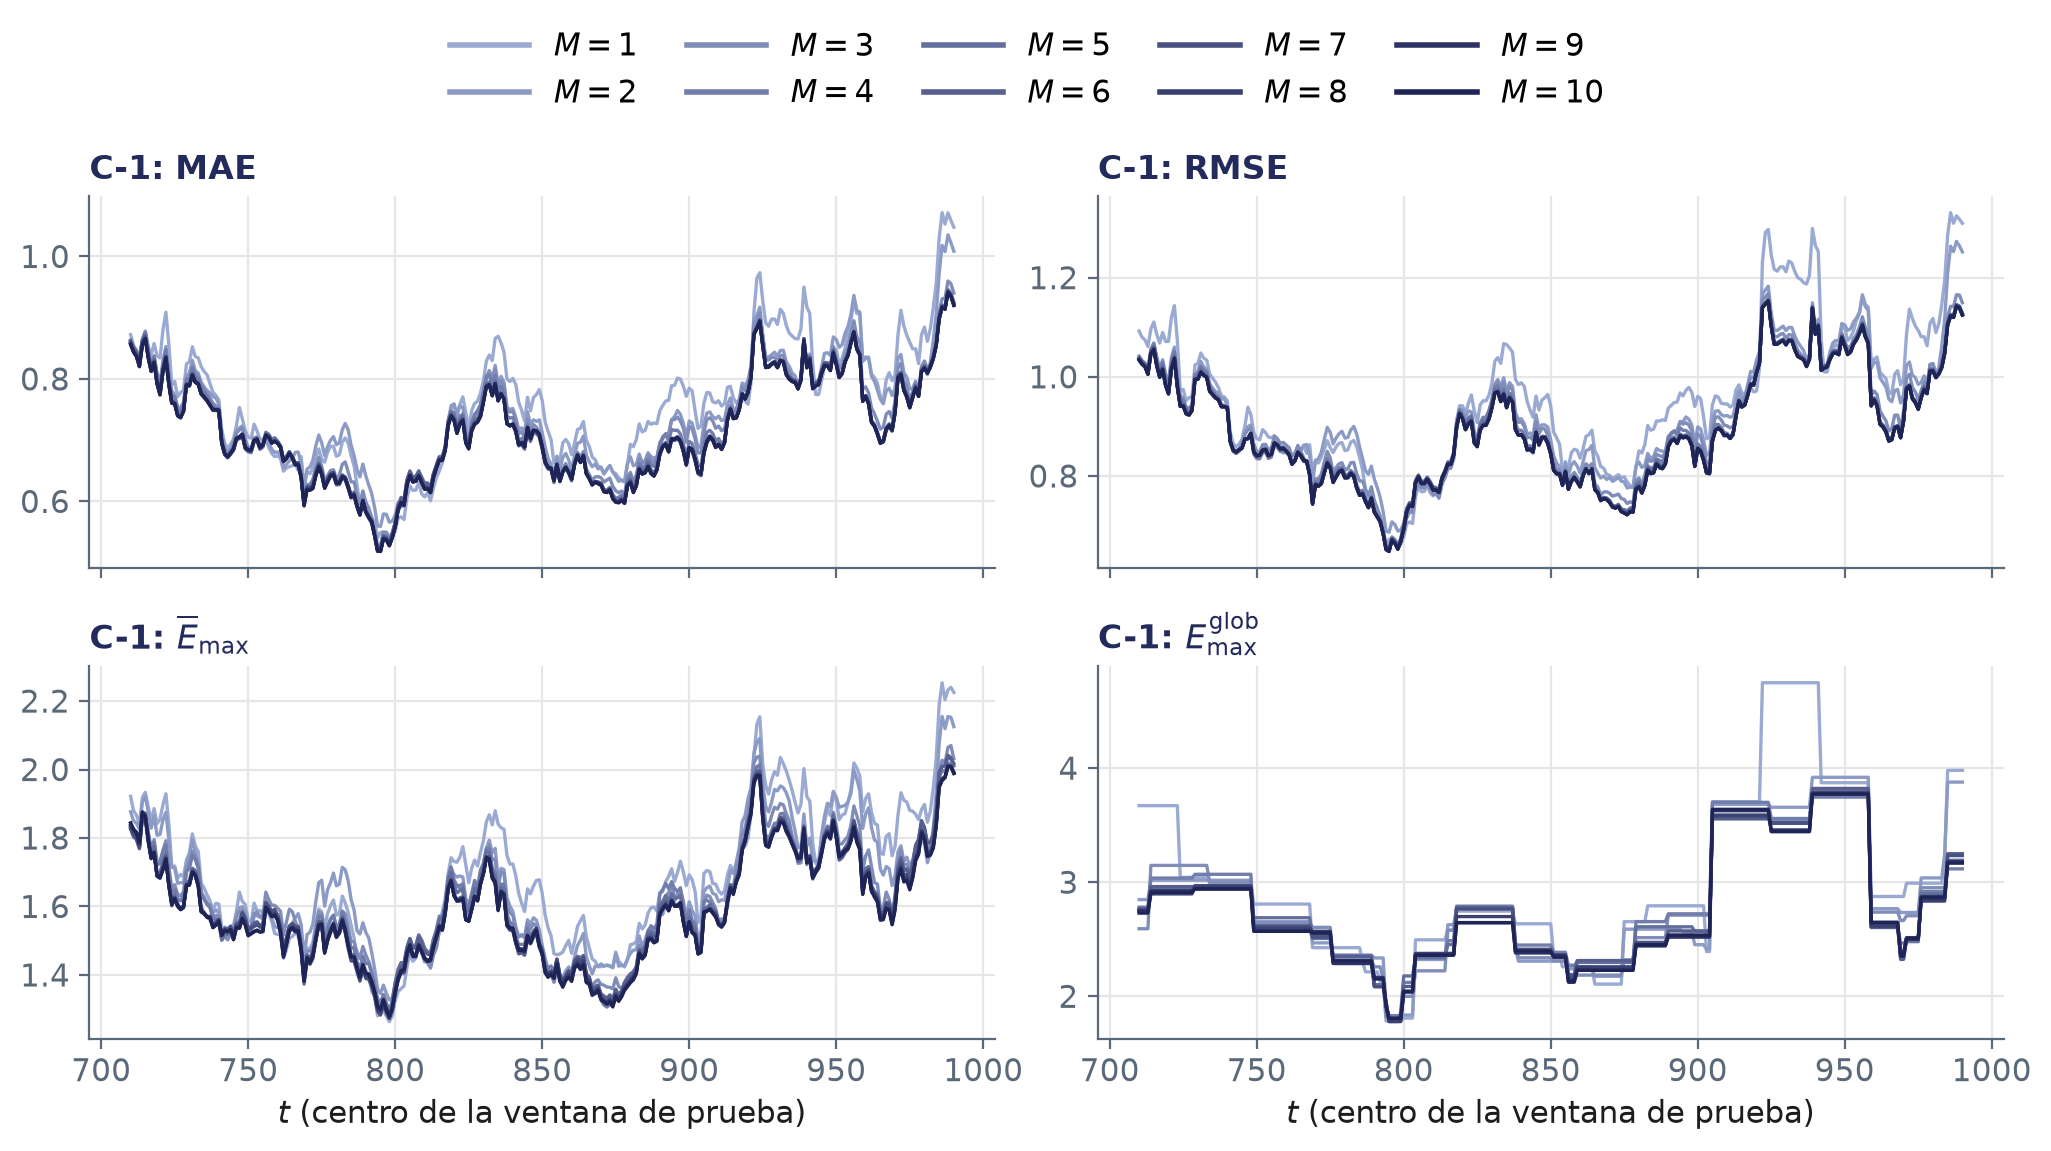
\includegraphics[width=\textwidth]{IMG/aneB_00/aneB_00_bloqueA_w20_C1.png}\end{minipage}\hfill
\begin{minipage}{0.49\textwidth}\centering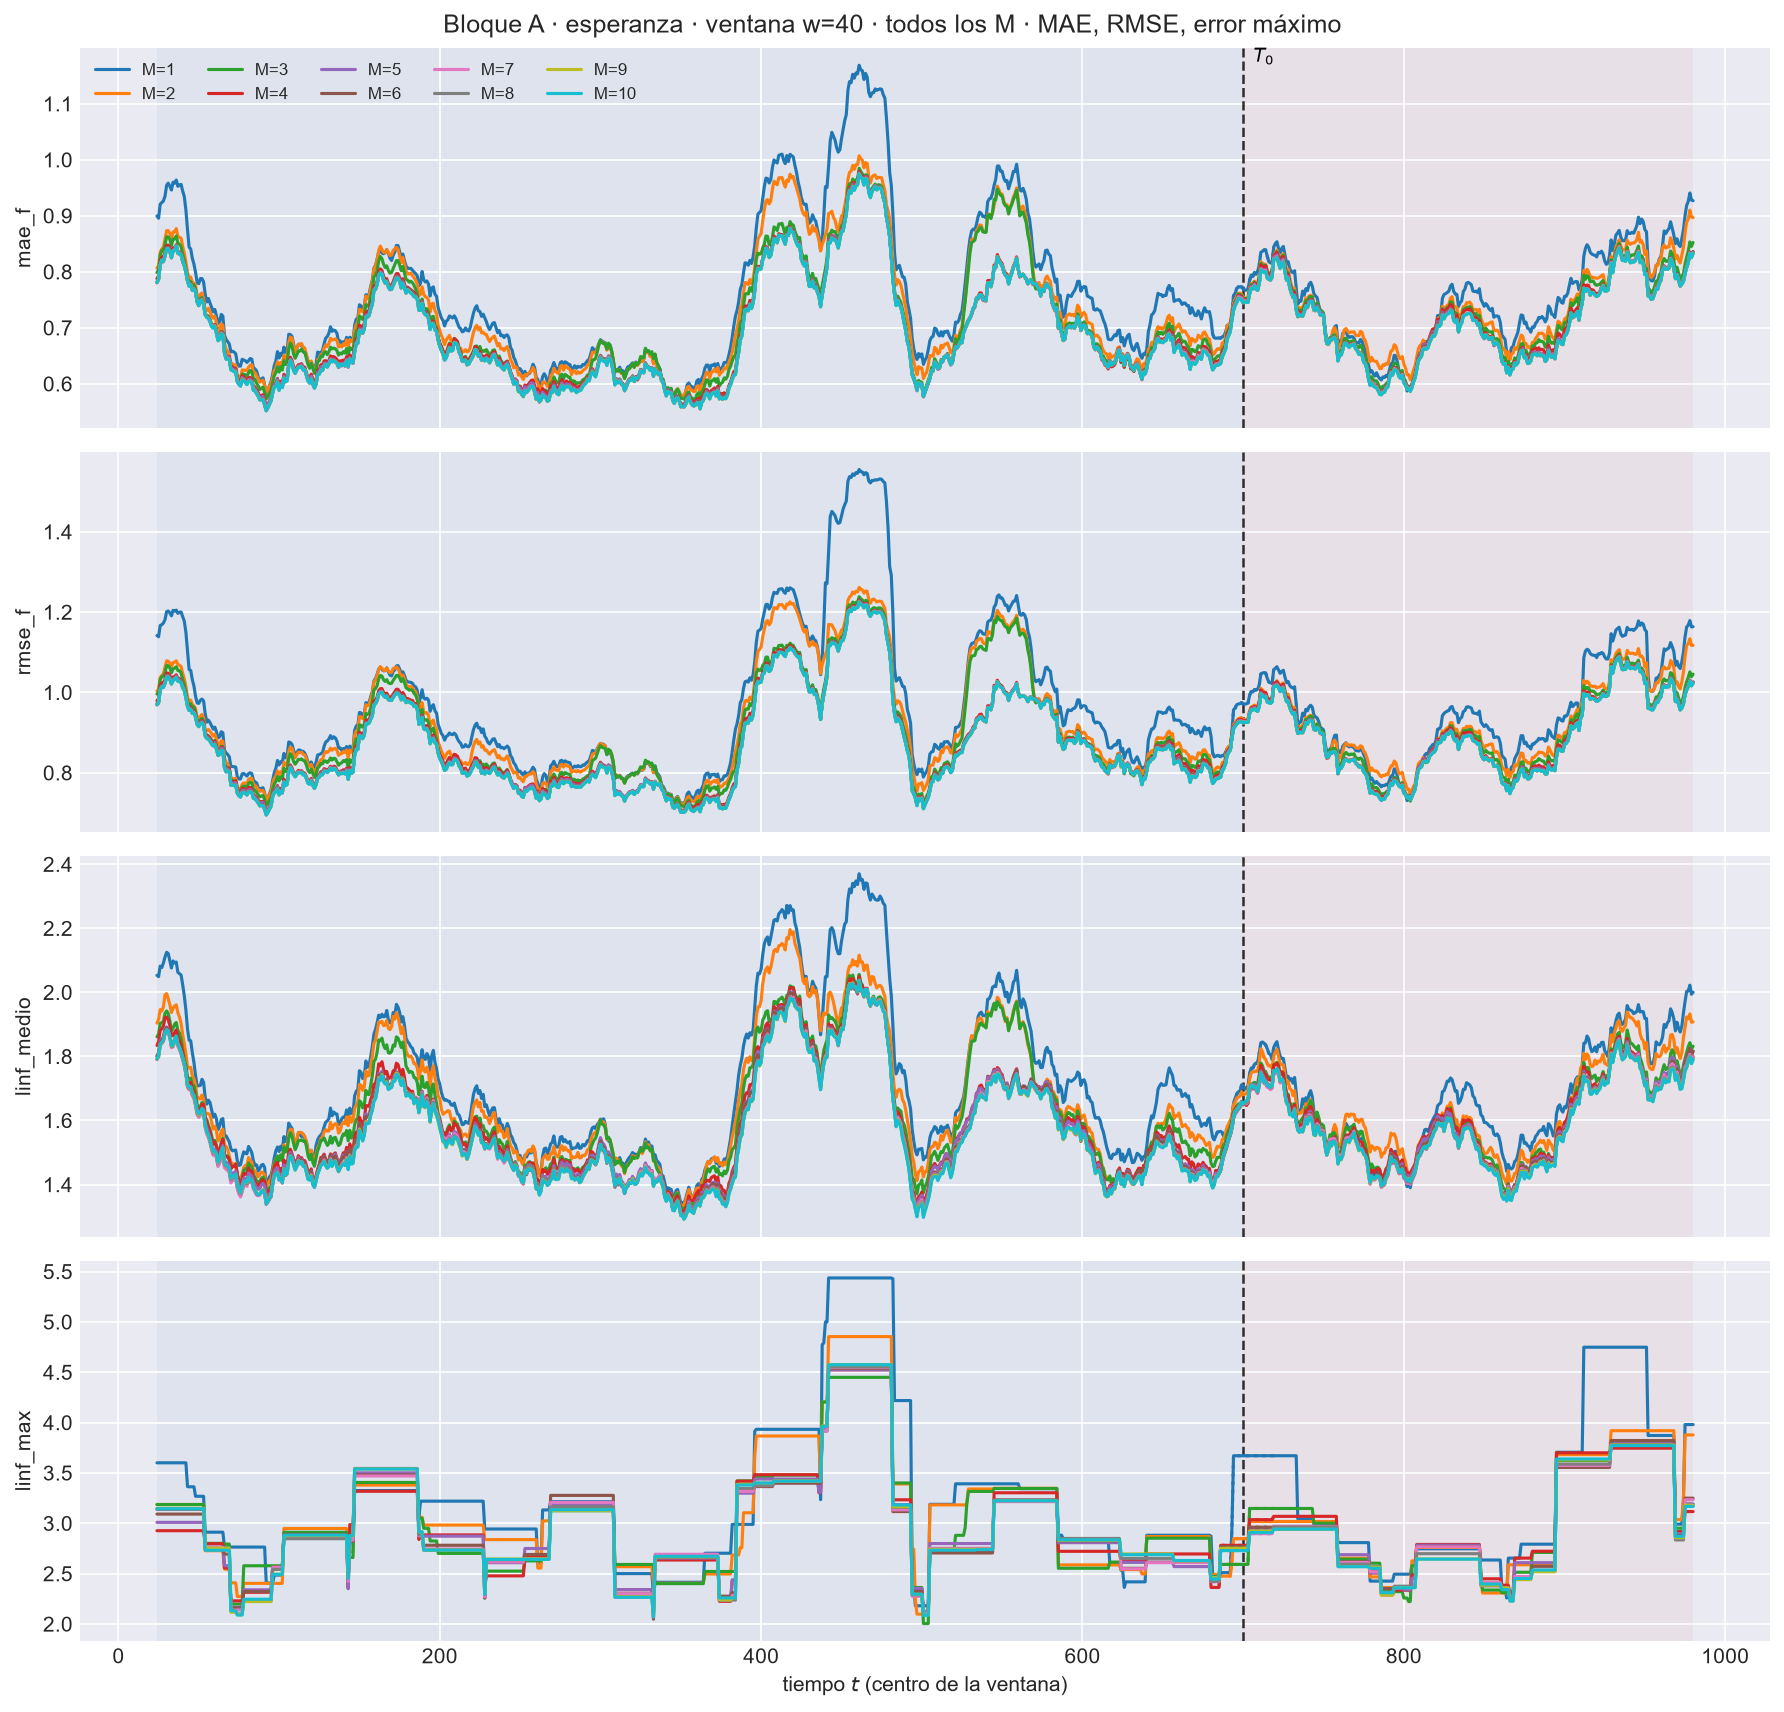
\includegraphics[width=\textwidth]{IMG/aneB_00/aneB_00_bloqueA_w40_C1.png}\end{minipage}
\caption{C-1 (GARCH). Métricas de error sobre la ventana móvil con $w = 20$ (izquierda) y $w = 40$ (derecha).}
\label{fig:aneB_ancho_A_C1}
\end{figure}

\begin{figure}[H]
\centering
\begin{minipage}{0.49\textwidth}\centering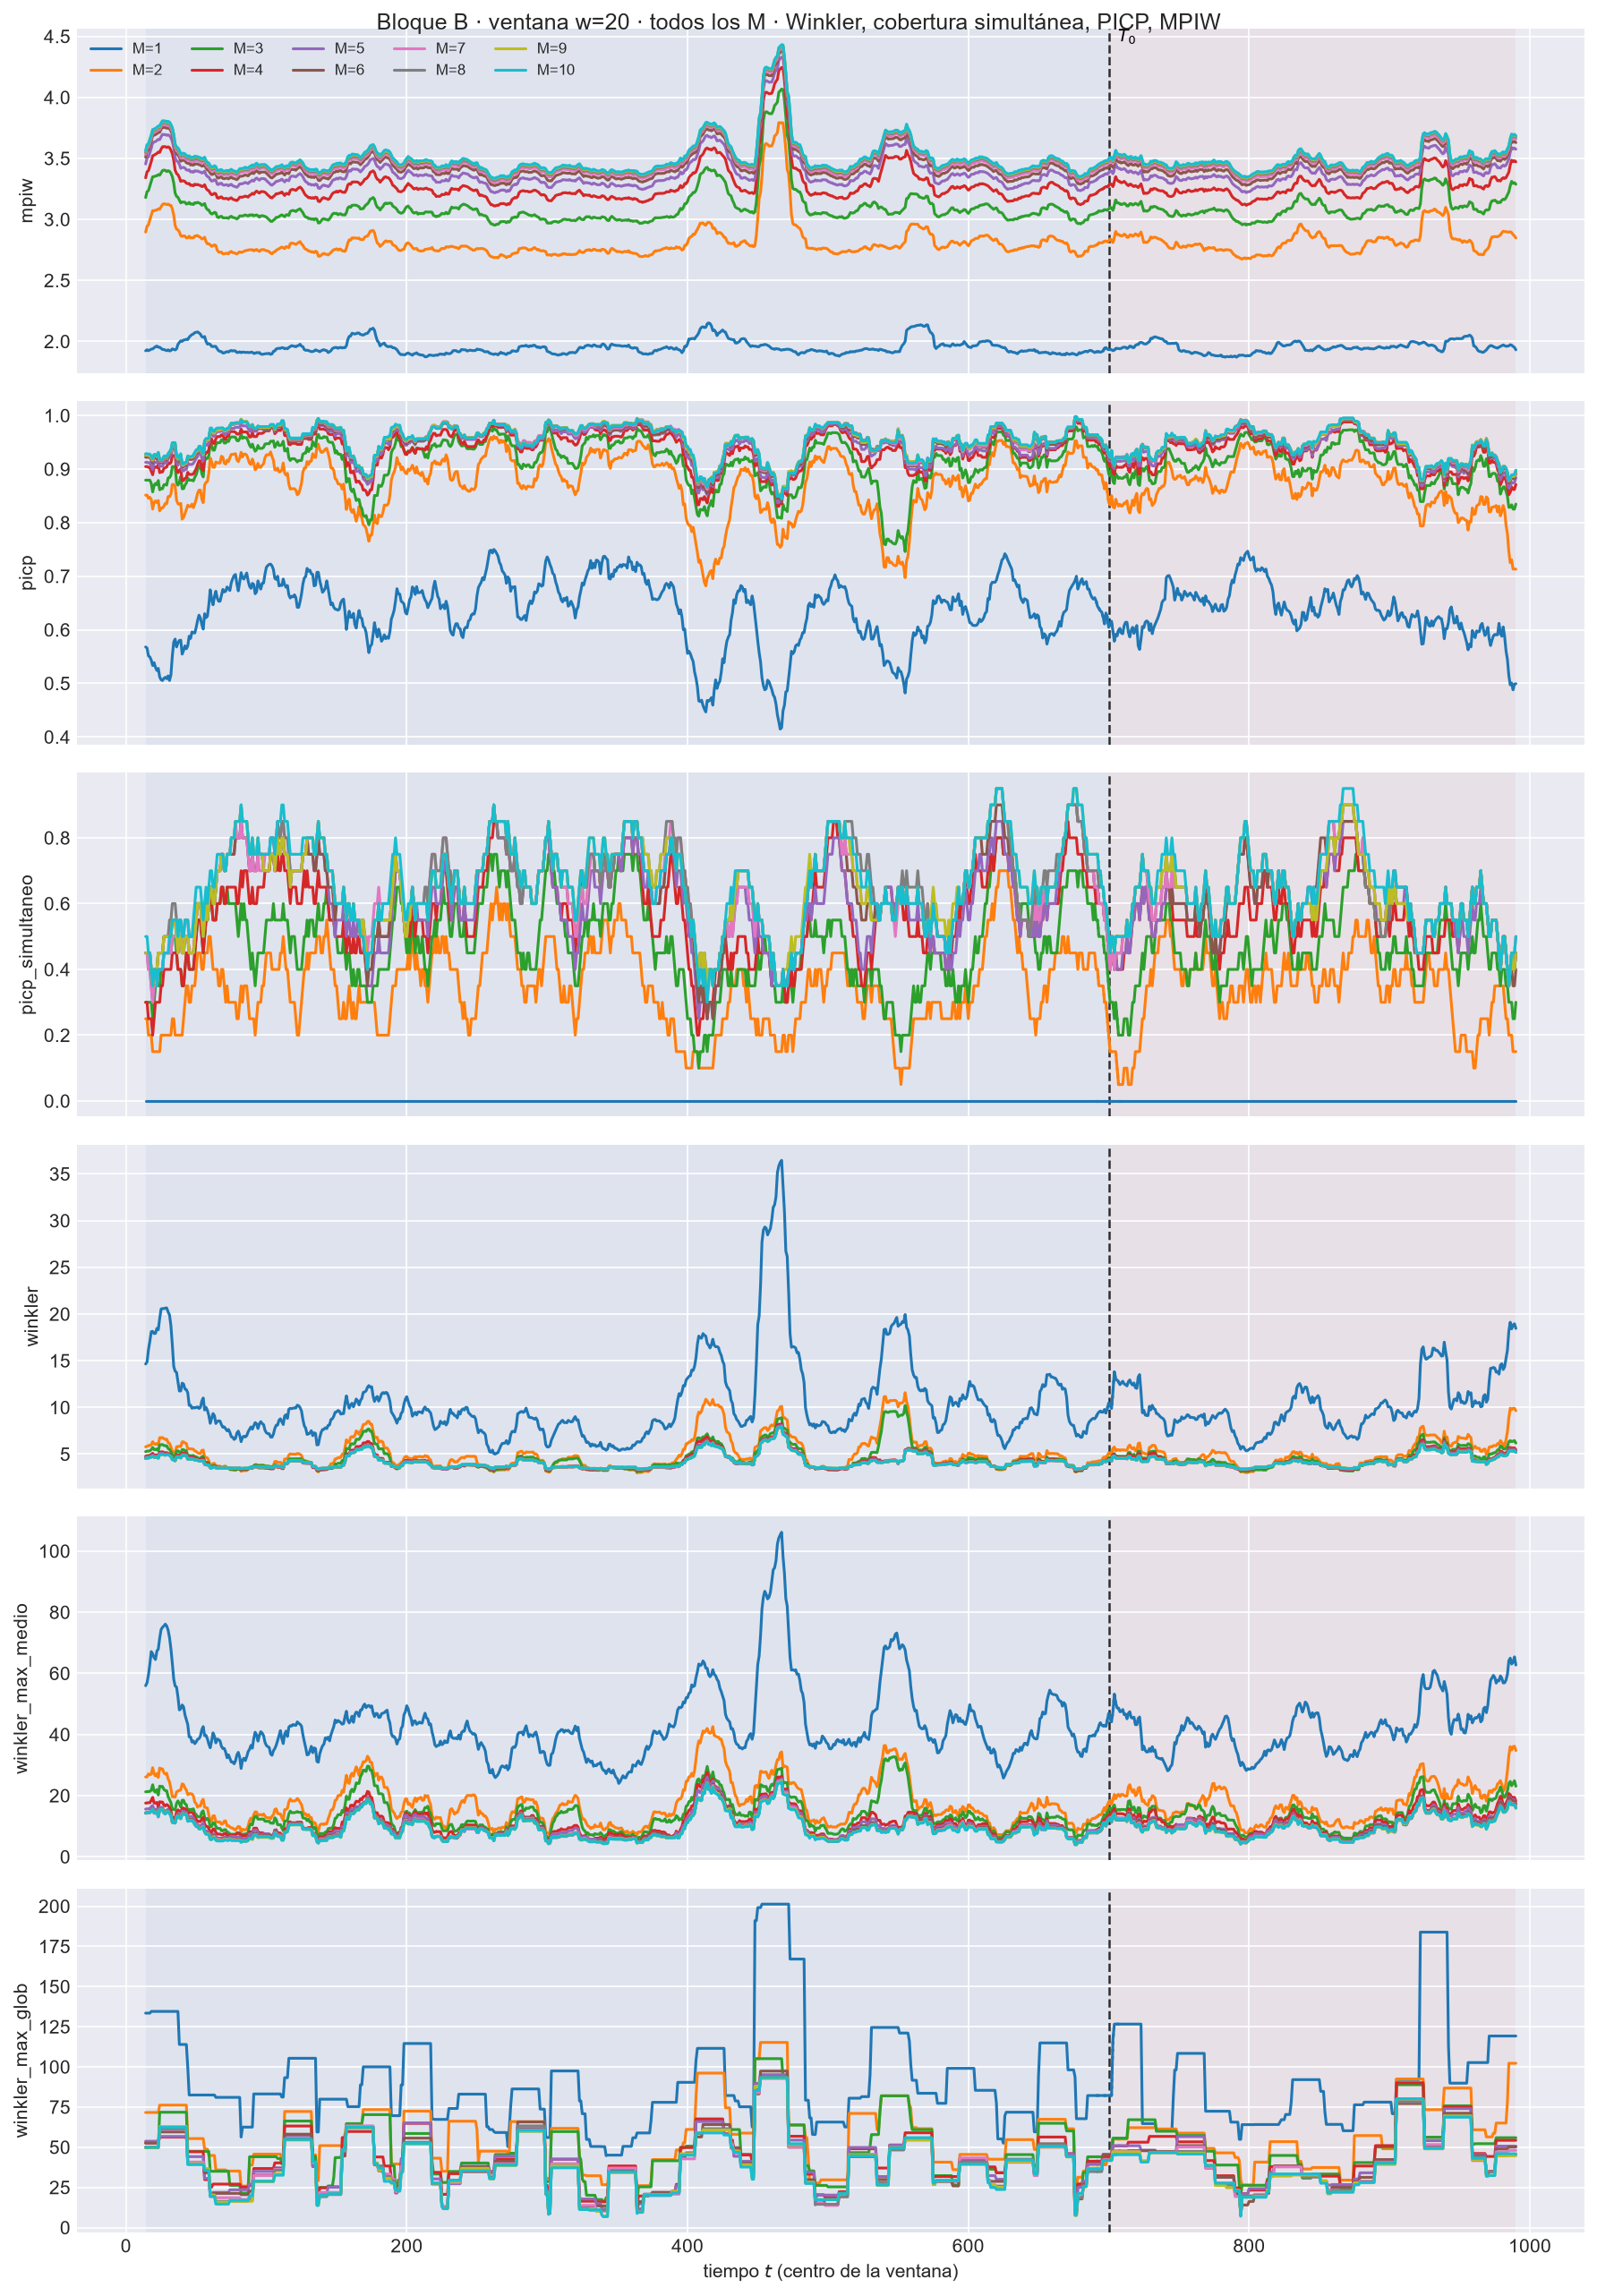
\includegraphics[width=\textwidth]{IMG/aneB_00/aneB_00_bloqueB_w20_C1.png}\end{minipage}\hfill
\begin{minipage}{0.49\textwidth}\centering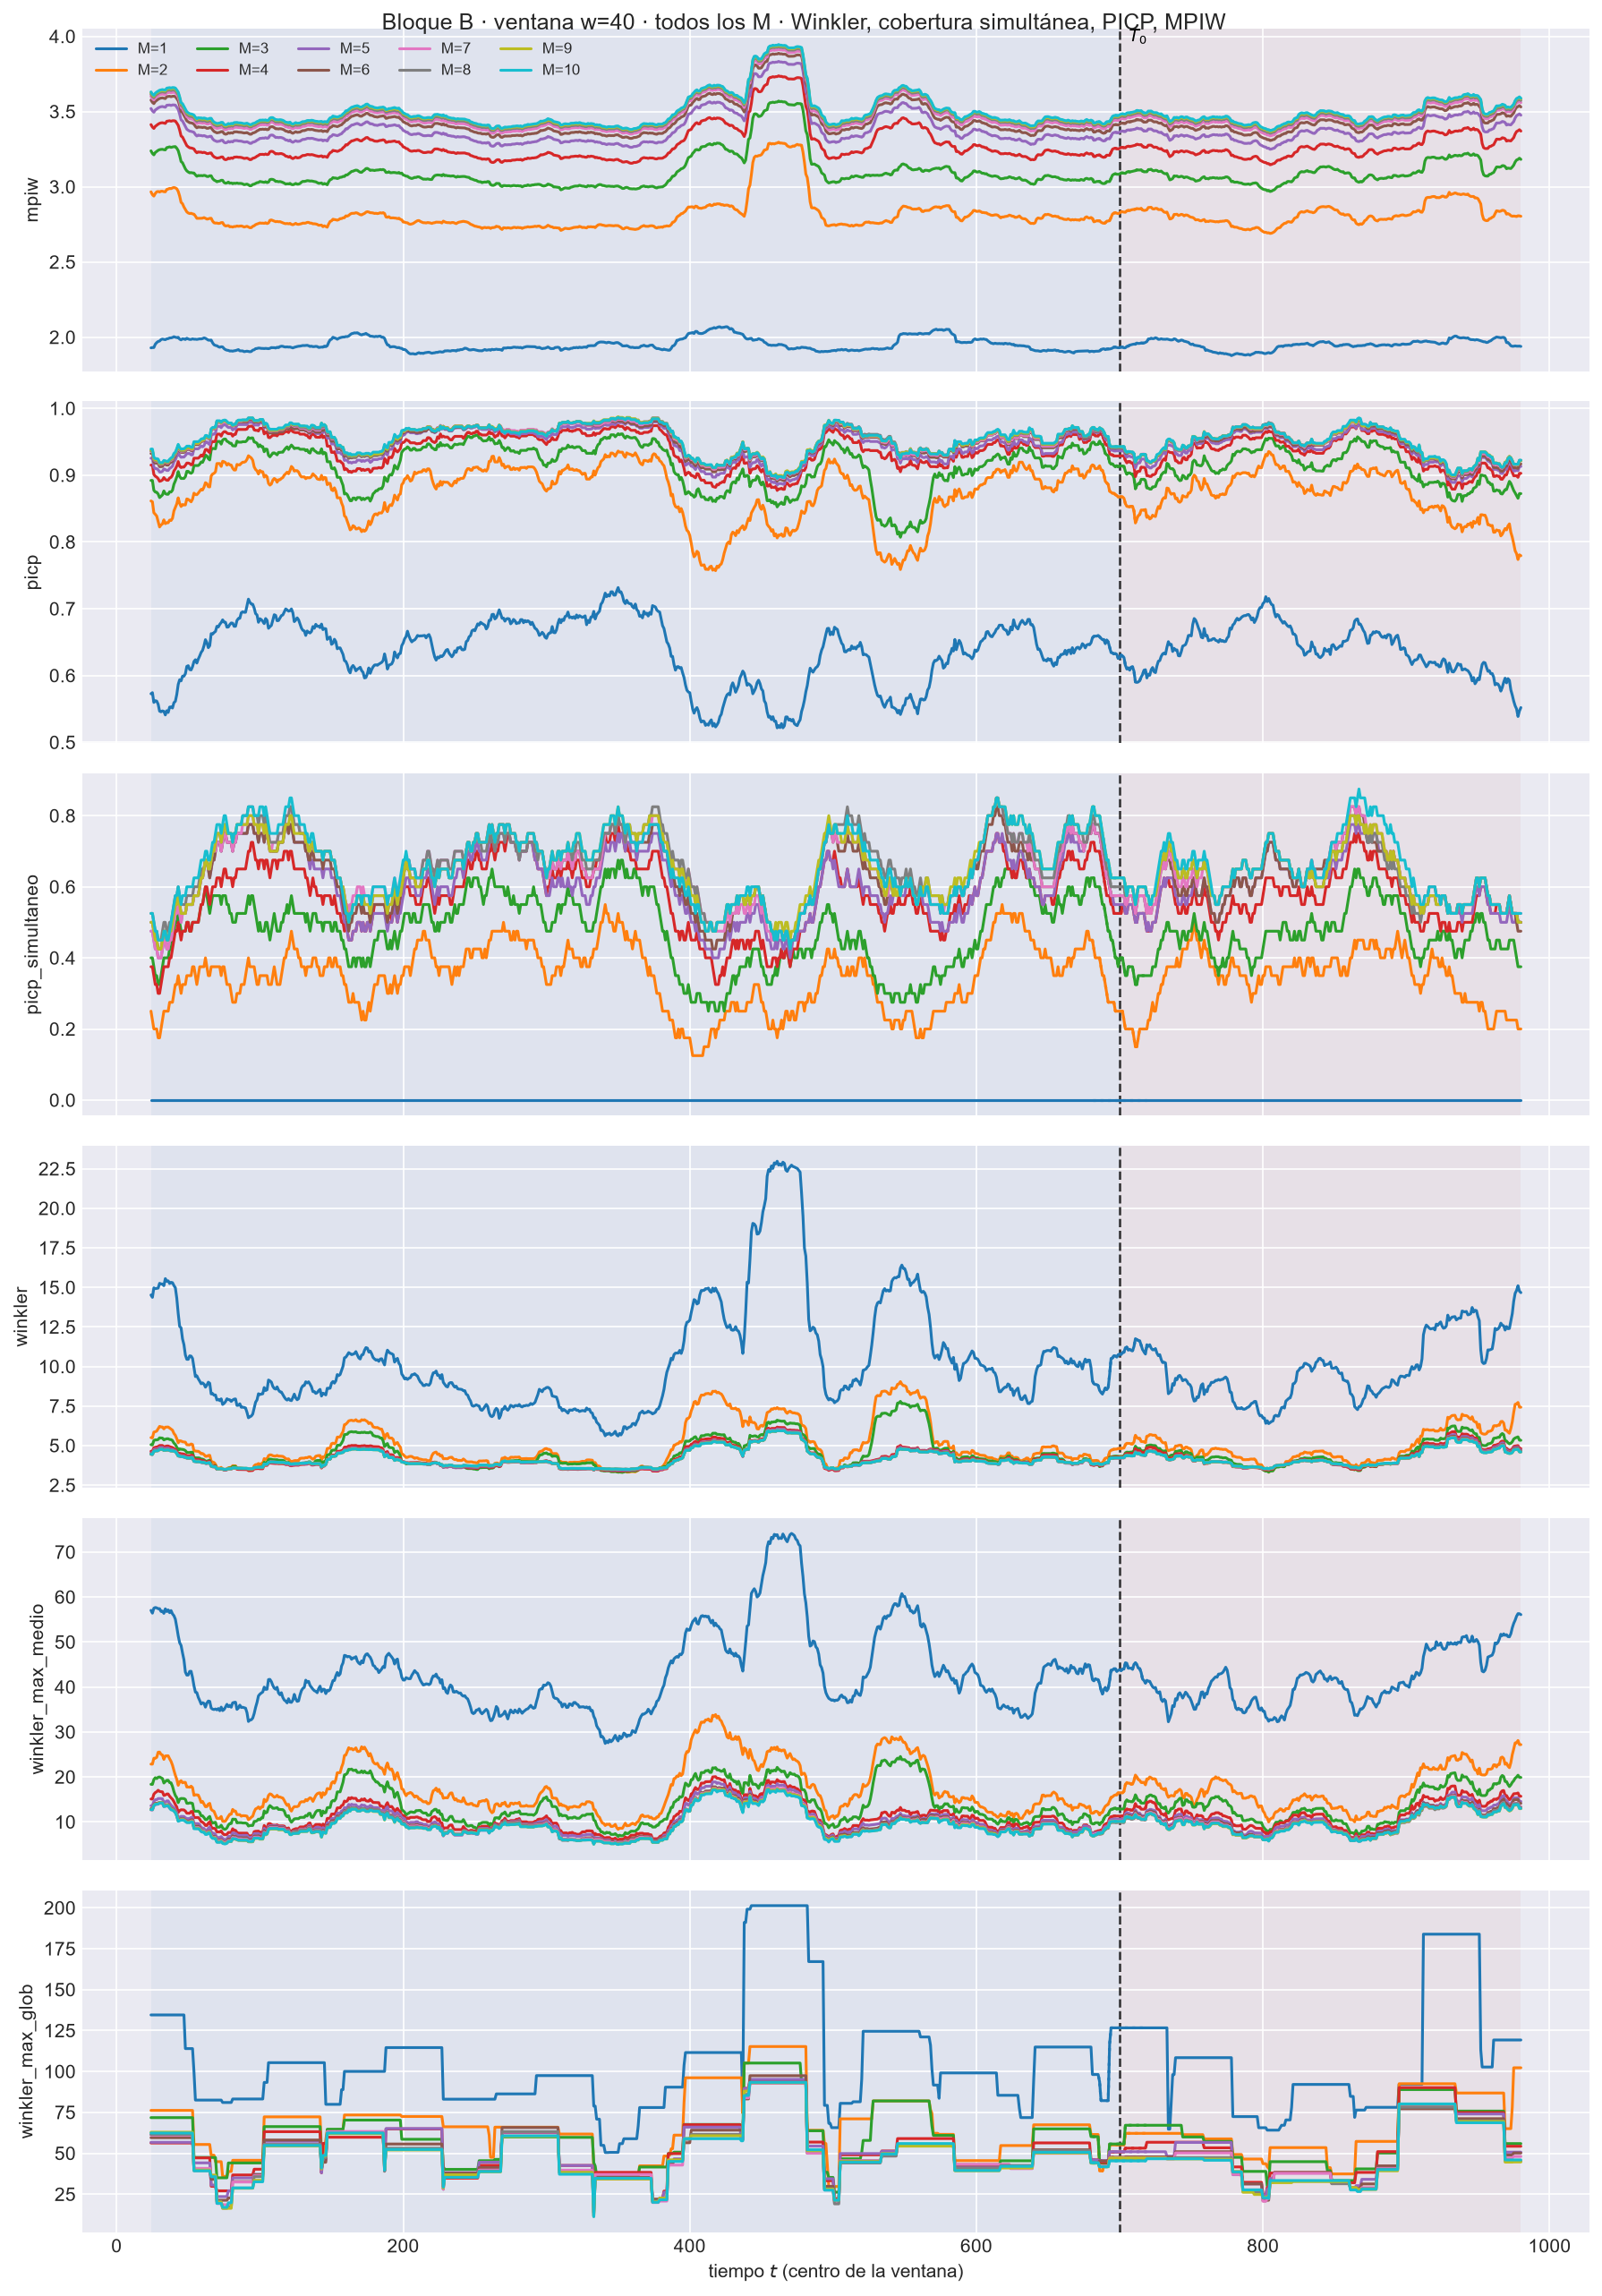
\includegraphics[width=\textwidth]{IMG/aneB_00/aneB_00_bloqueB_w40_C1.png}\end{minipage}
\caption{C-1 (GARCH). Métricas de intervalo sobre la ventana móvil con $w = 20$ (izquierda) y $w = 40$ (derecha).}
\label{fig:aneB_ancho_B_C1}
\end{figure}

\begin{figure}[H]
\centering
\begin{minipage}{0.49\textwidth}\centering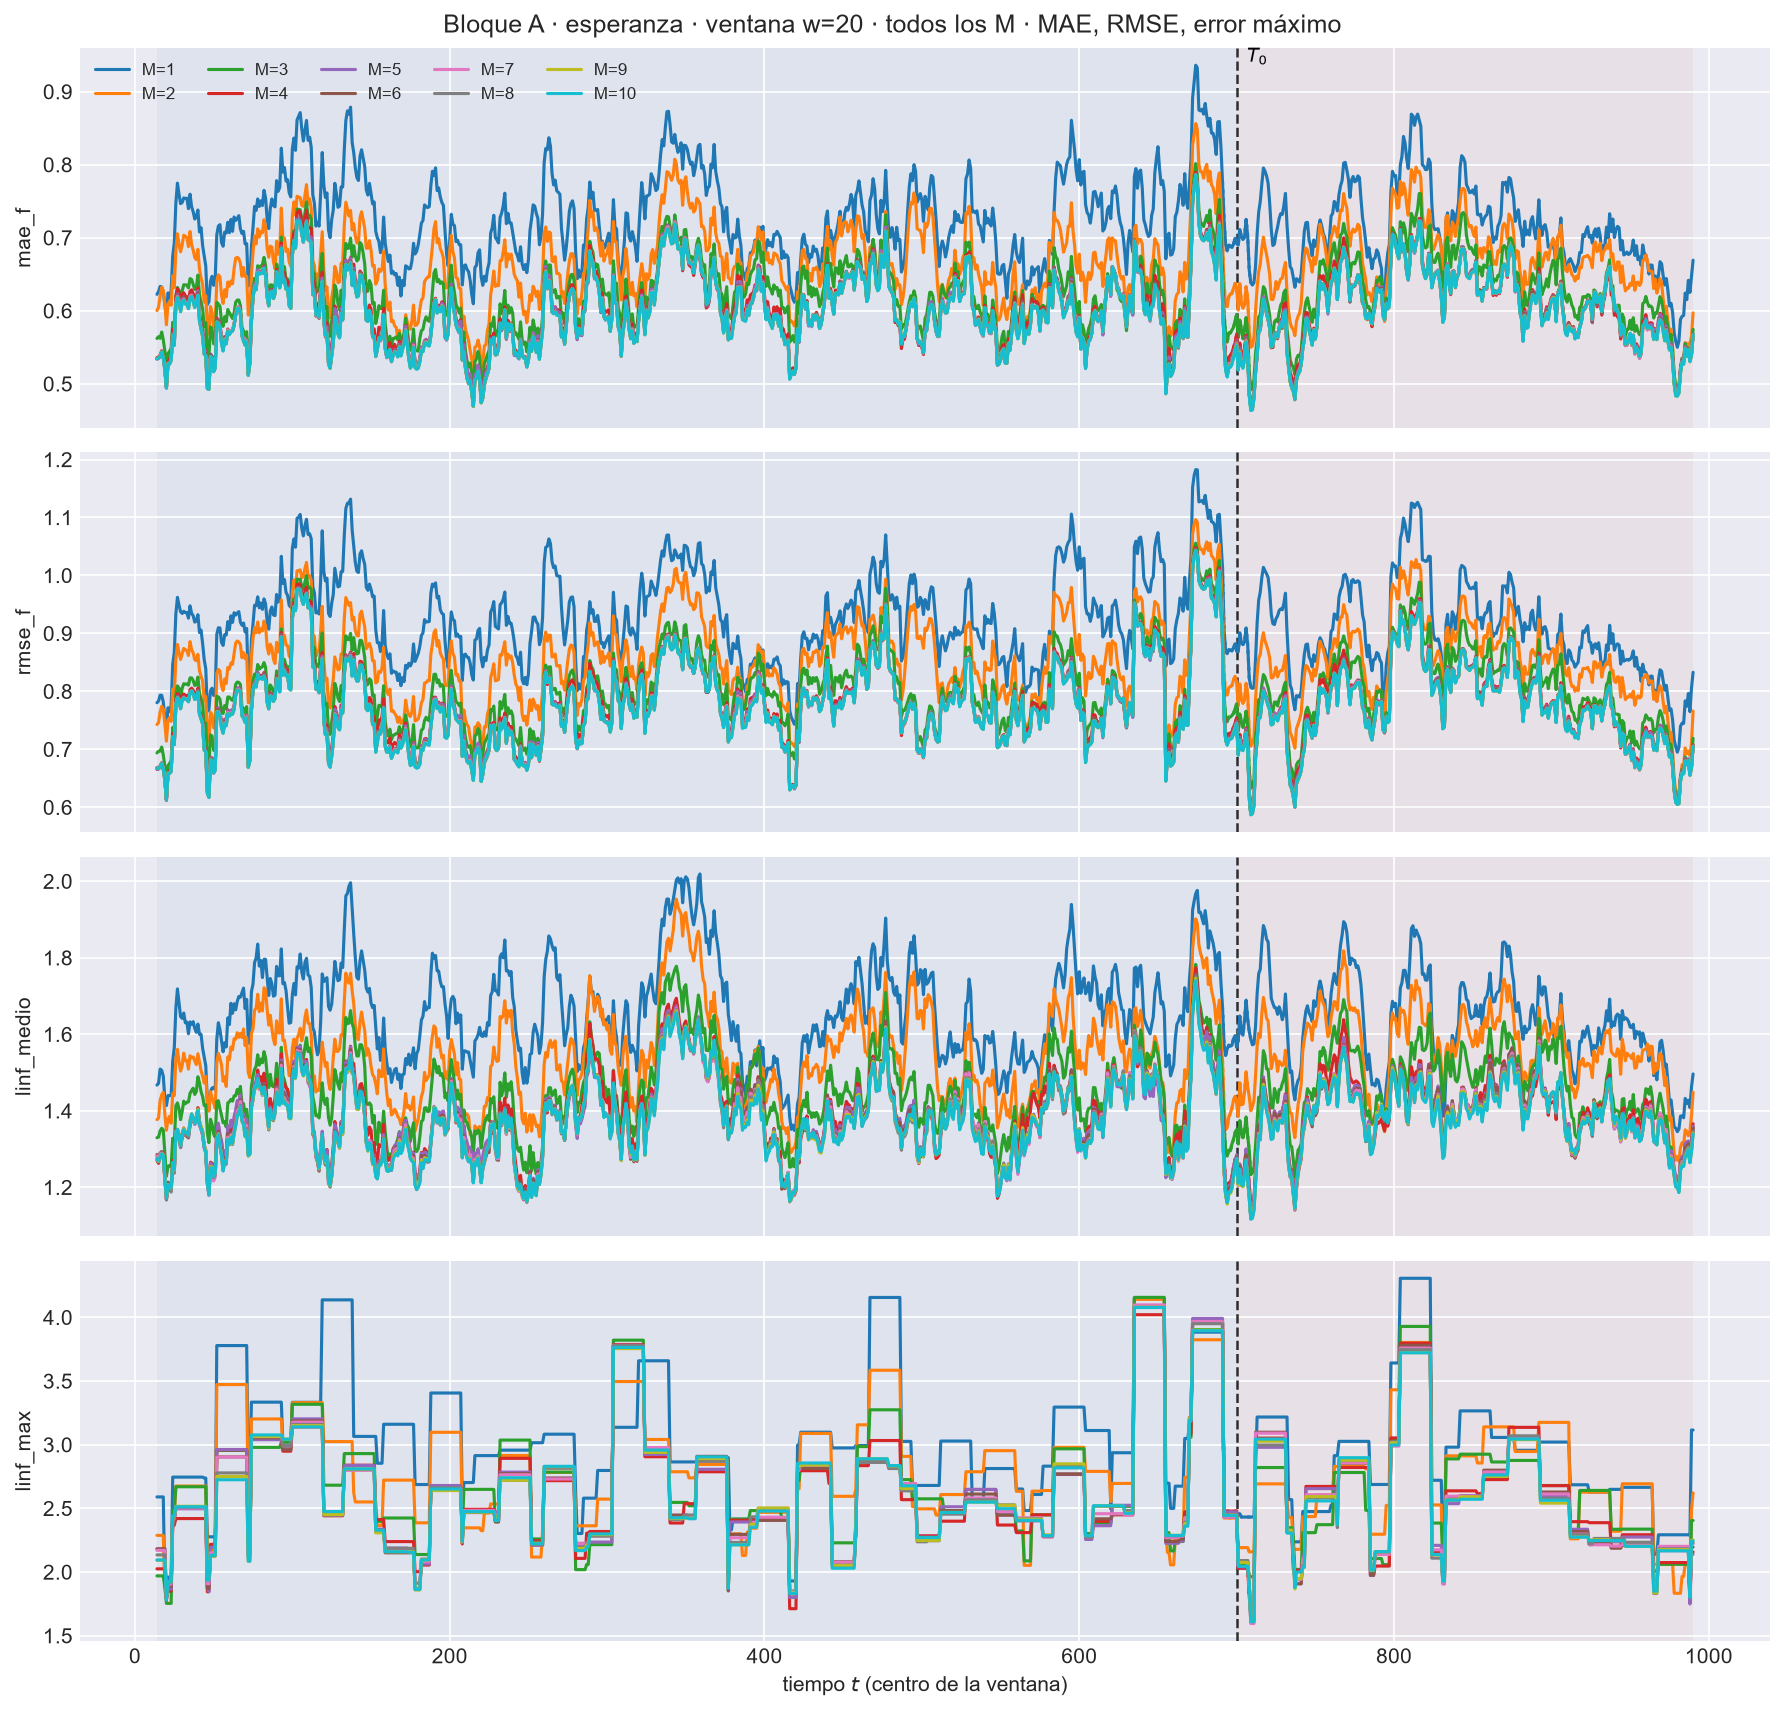
\includegraphics[width=\textwidth]{IMG/aneB_00/aneB_00_bloqueA_w20_C2.png}\end{minipage}\hfill
\begin{minipage}{0.49\textwidth}\centering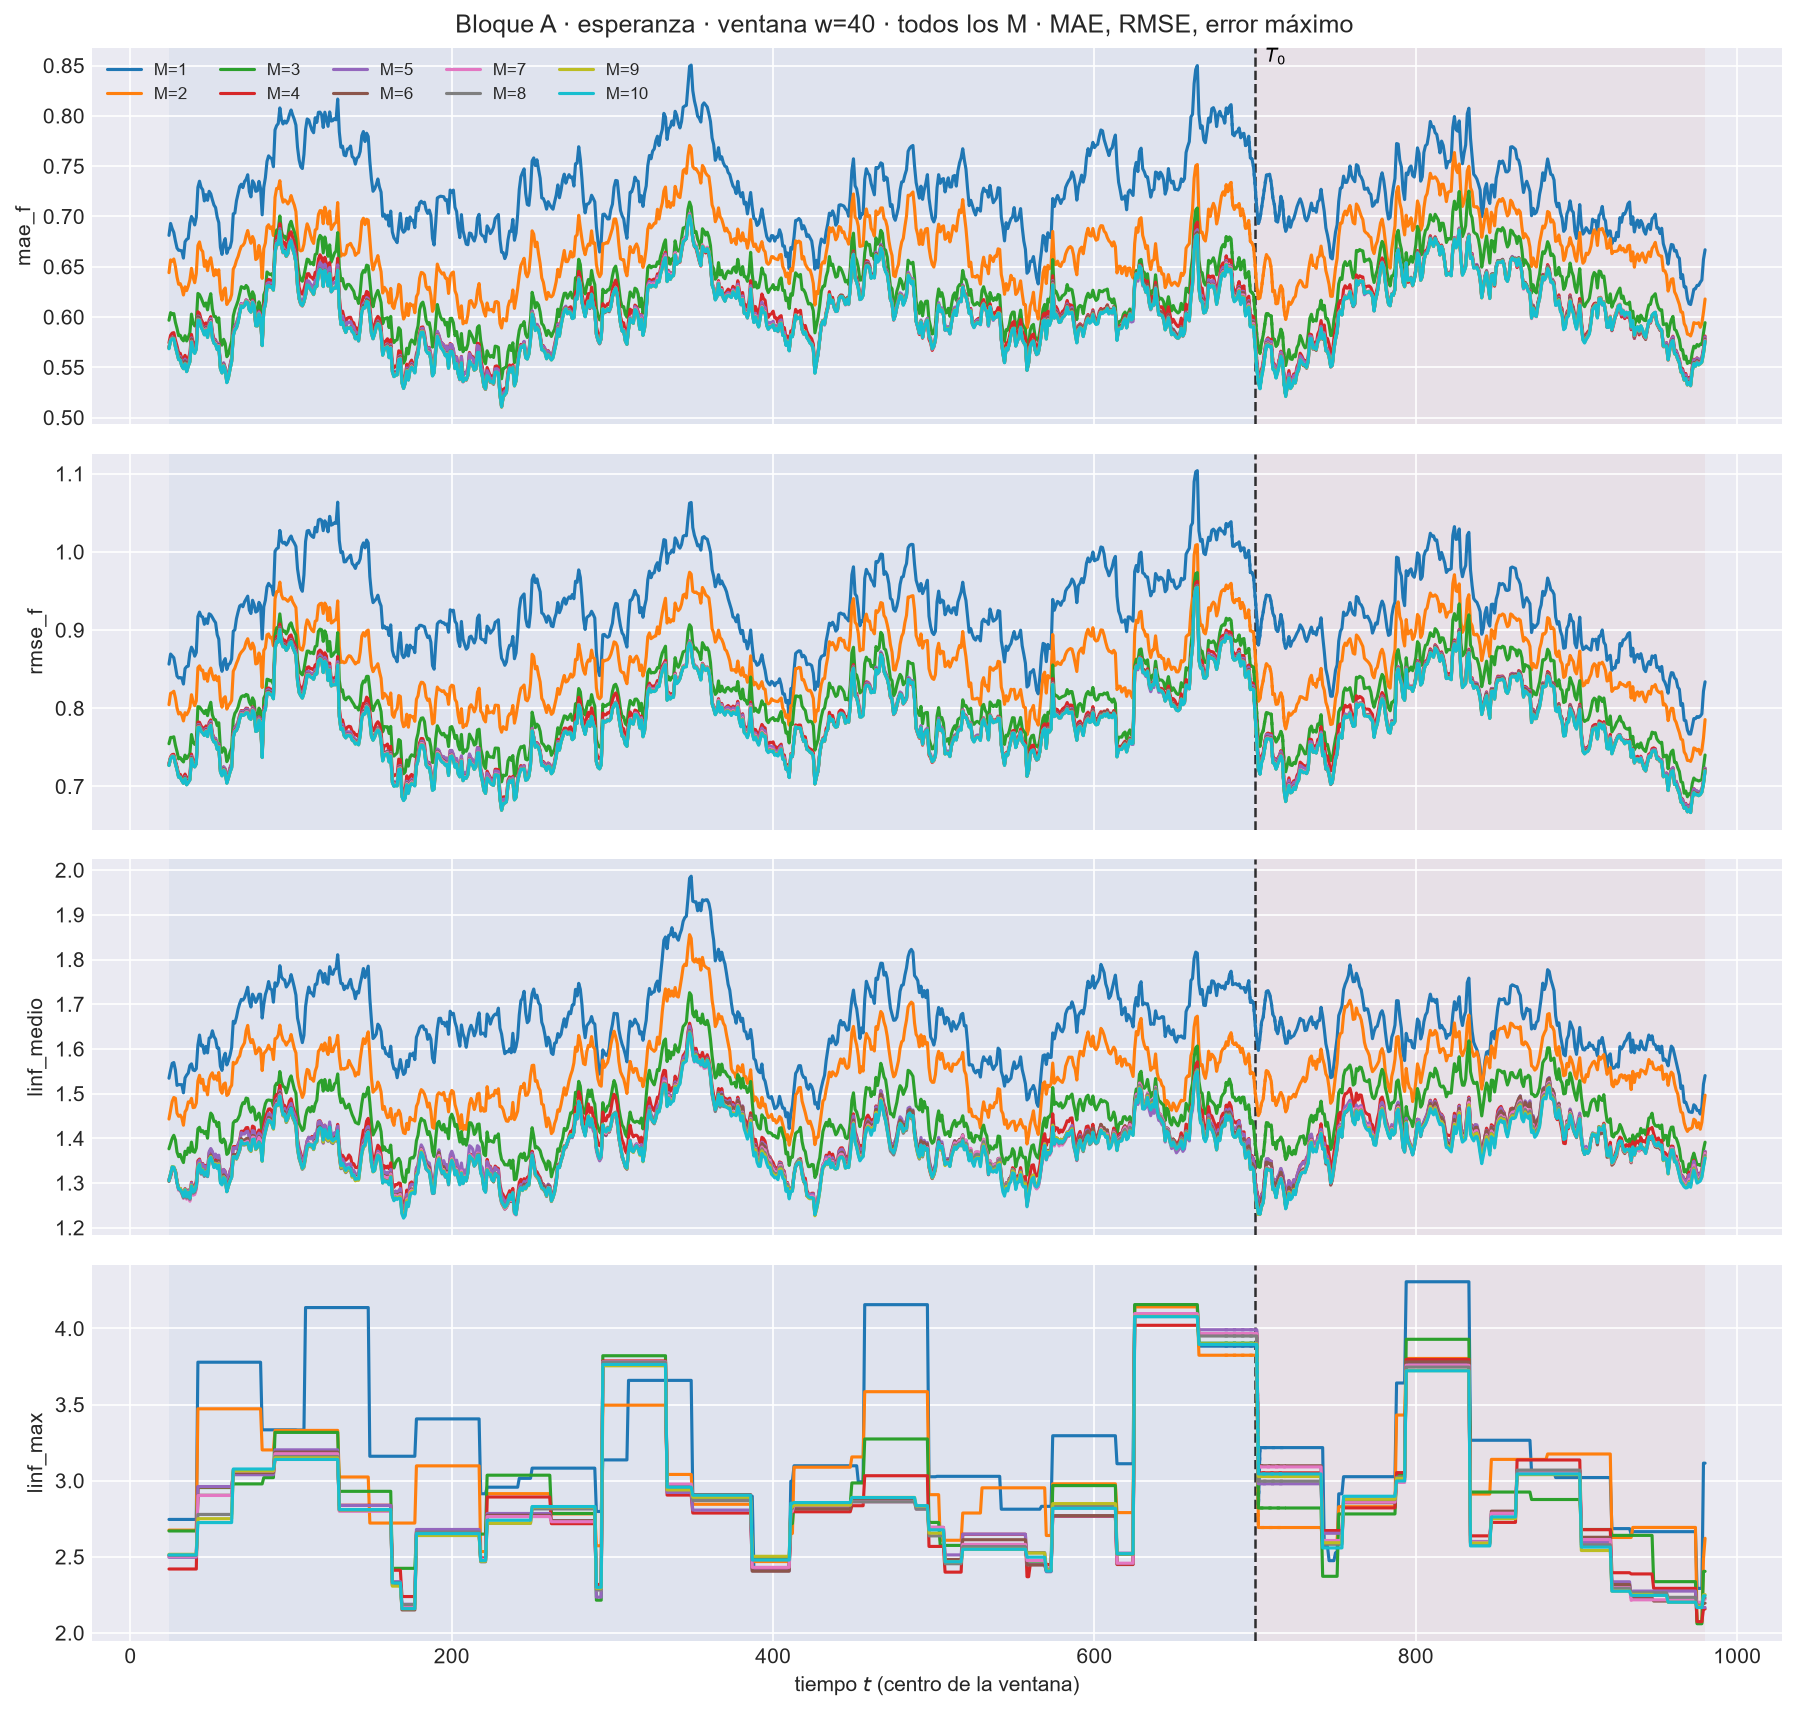
\includegraphics[width=\textwidth]{IMG/aneB_00/aneB_00_bloqueA_w40_C2.png}\end{minipage}
\caption{C-2 (TAR). Métricas de error sobre la ventana móvil con $w = 20$ (izquierda) y $w = 40$ (derecha).}
\label{fig:aneB_ancho_A_C2}
\end{figure}

\begin{figure}[H]
\centering
\begin{minipage}{0.49\textwidth}\centering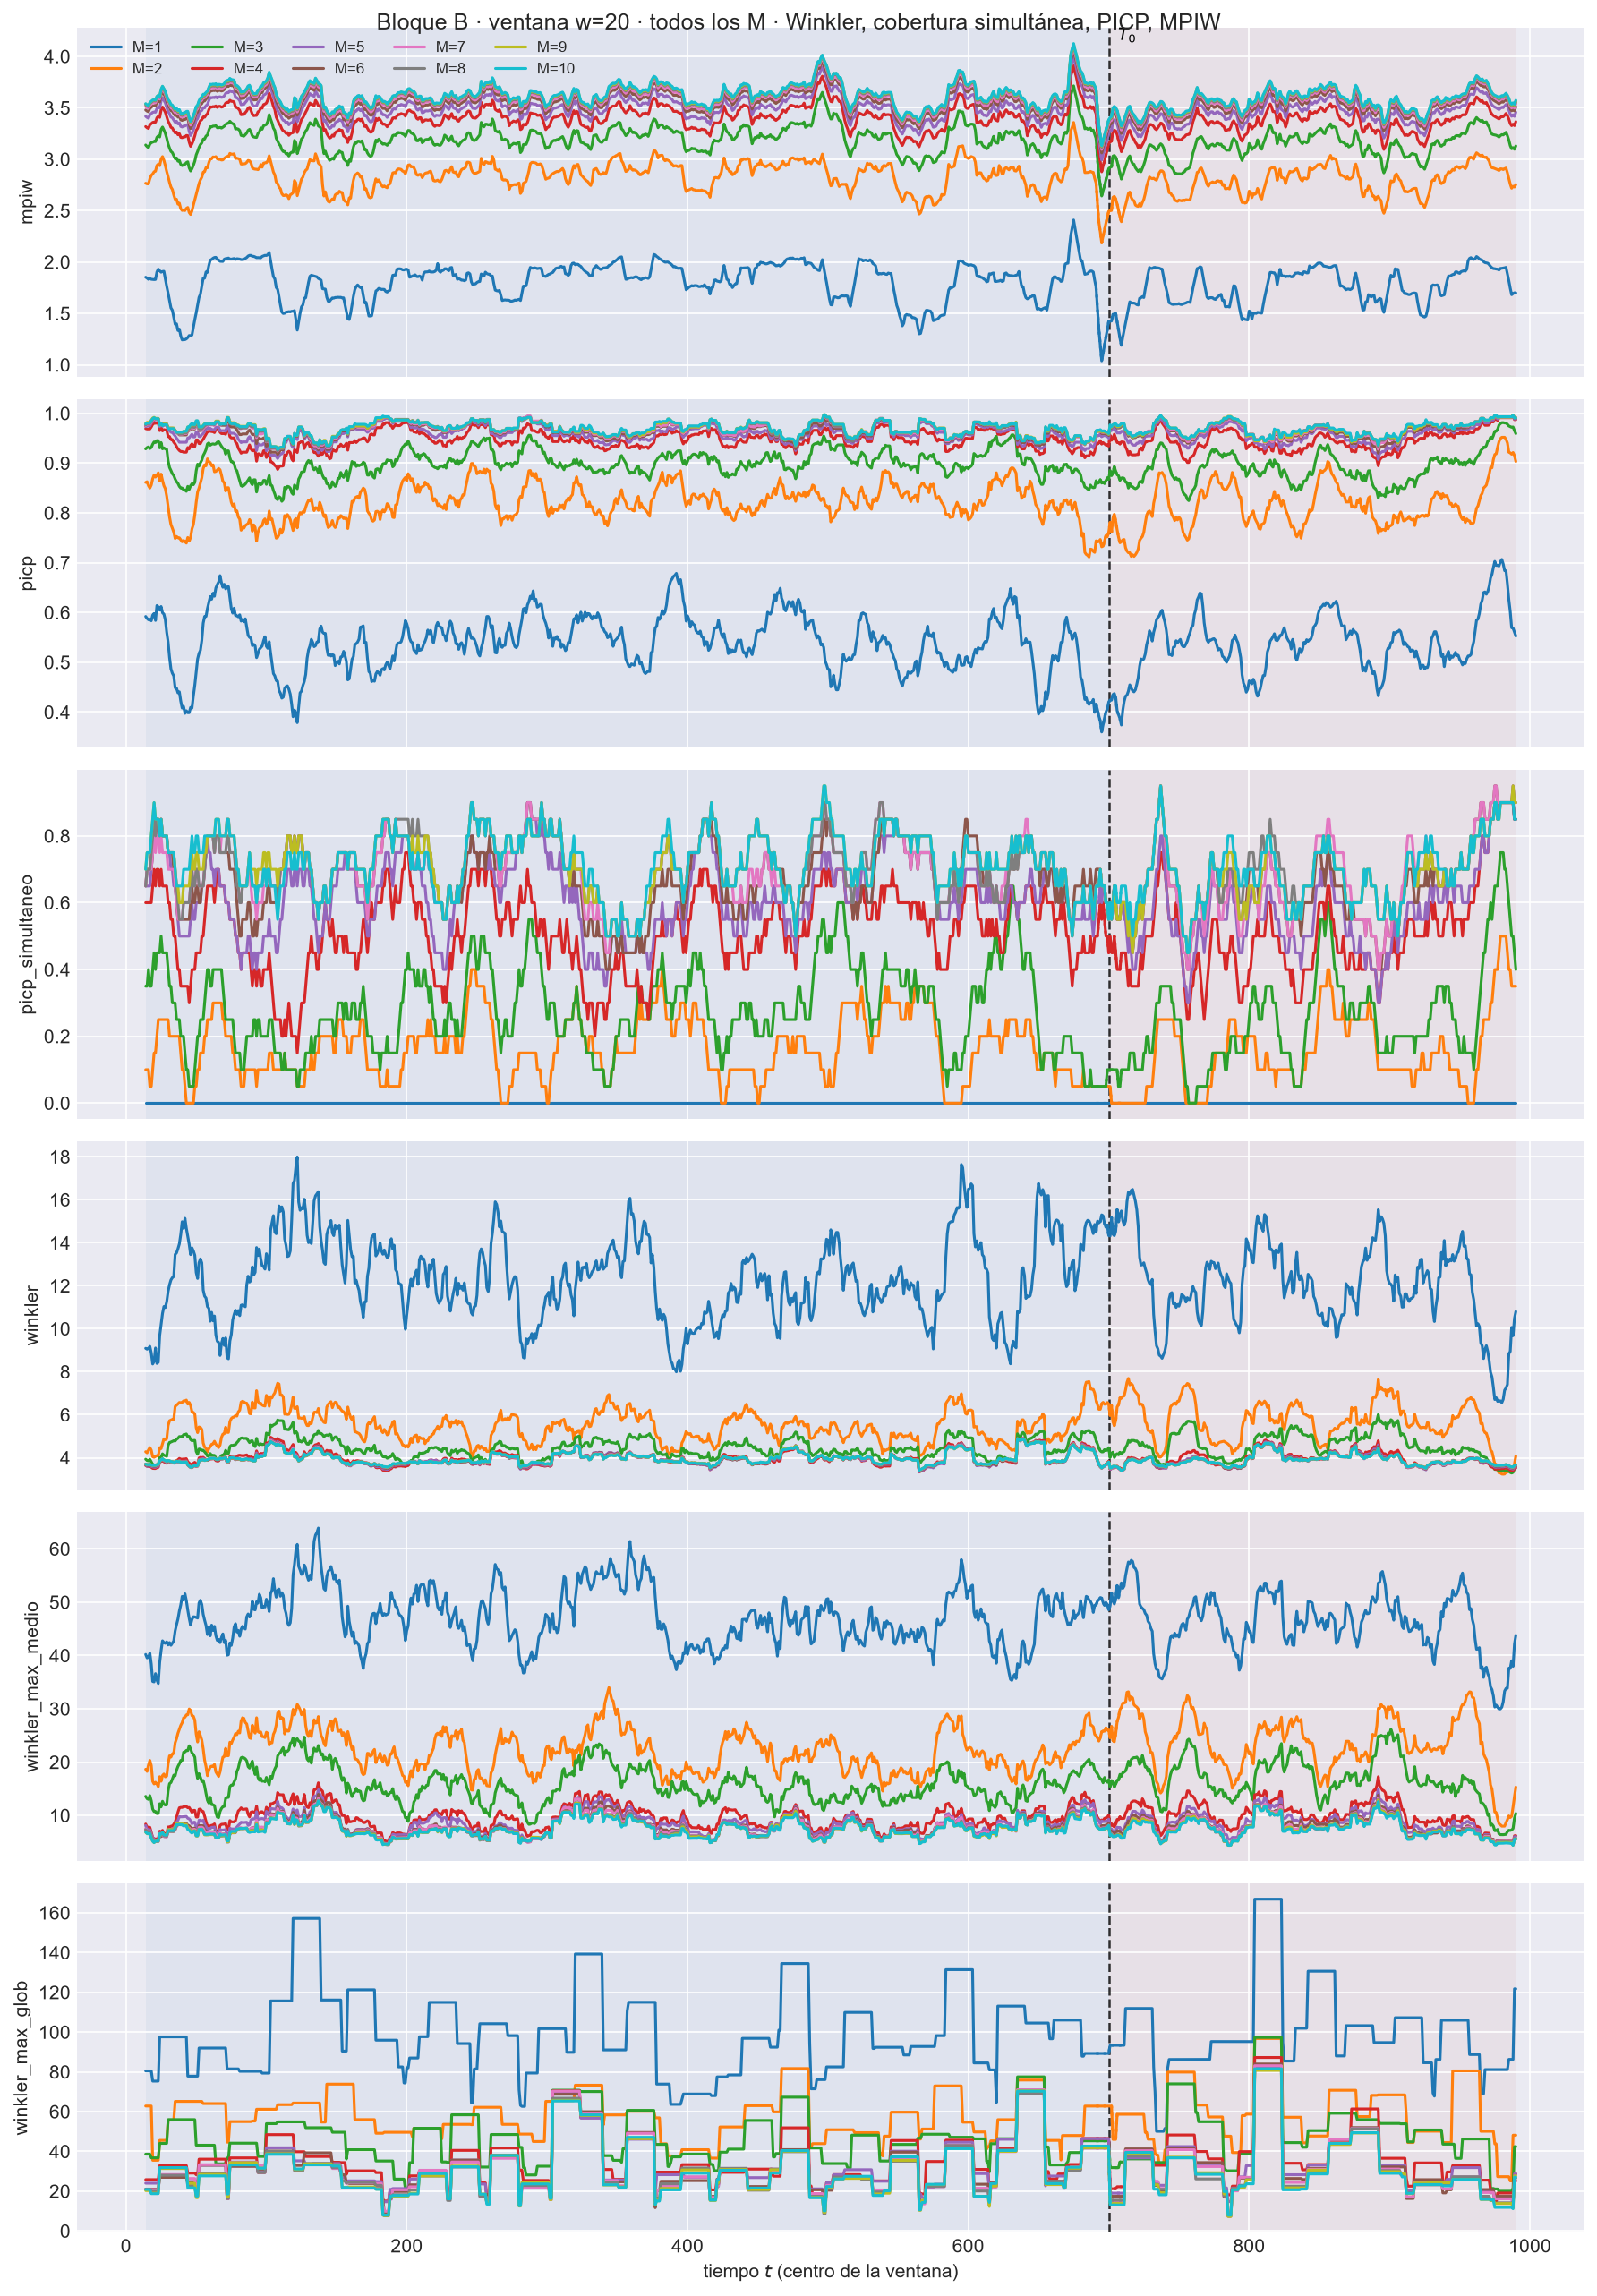
\includegraphics[width=\textwidth]{IMG/aneB_00/aneB_00_bloqueB_w20_C2.png}\end{minipage}\hfill
\begin{minipage}{0.49\textwidth}\centering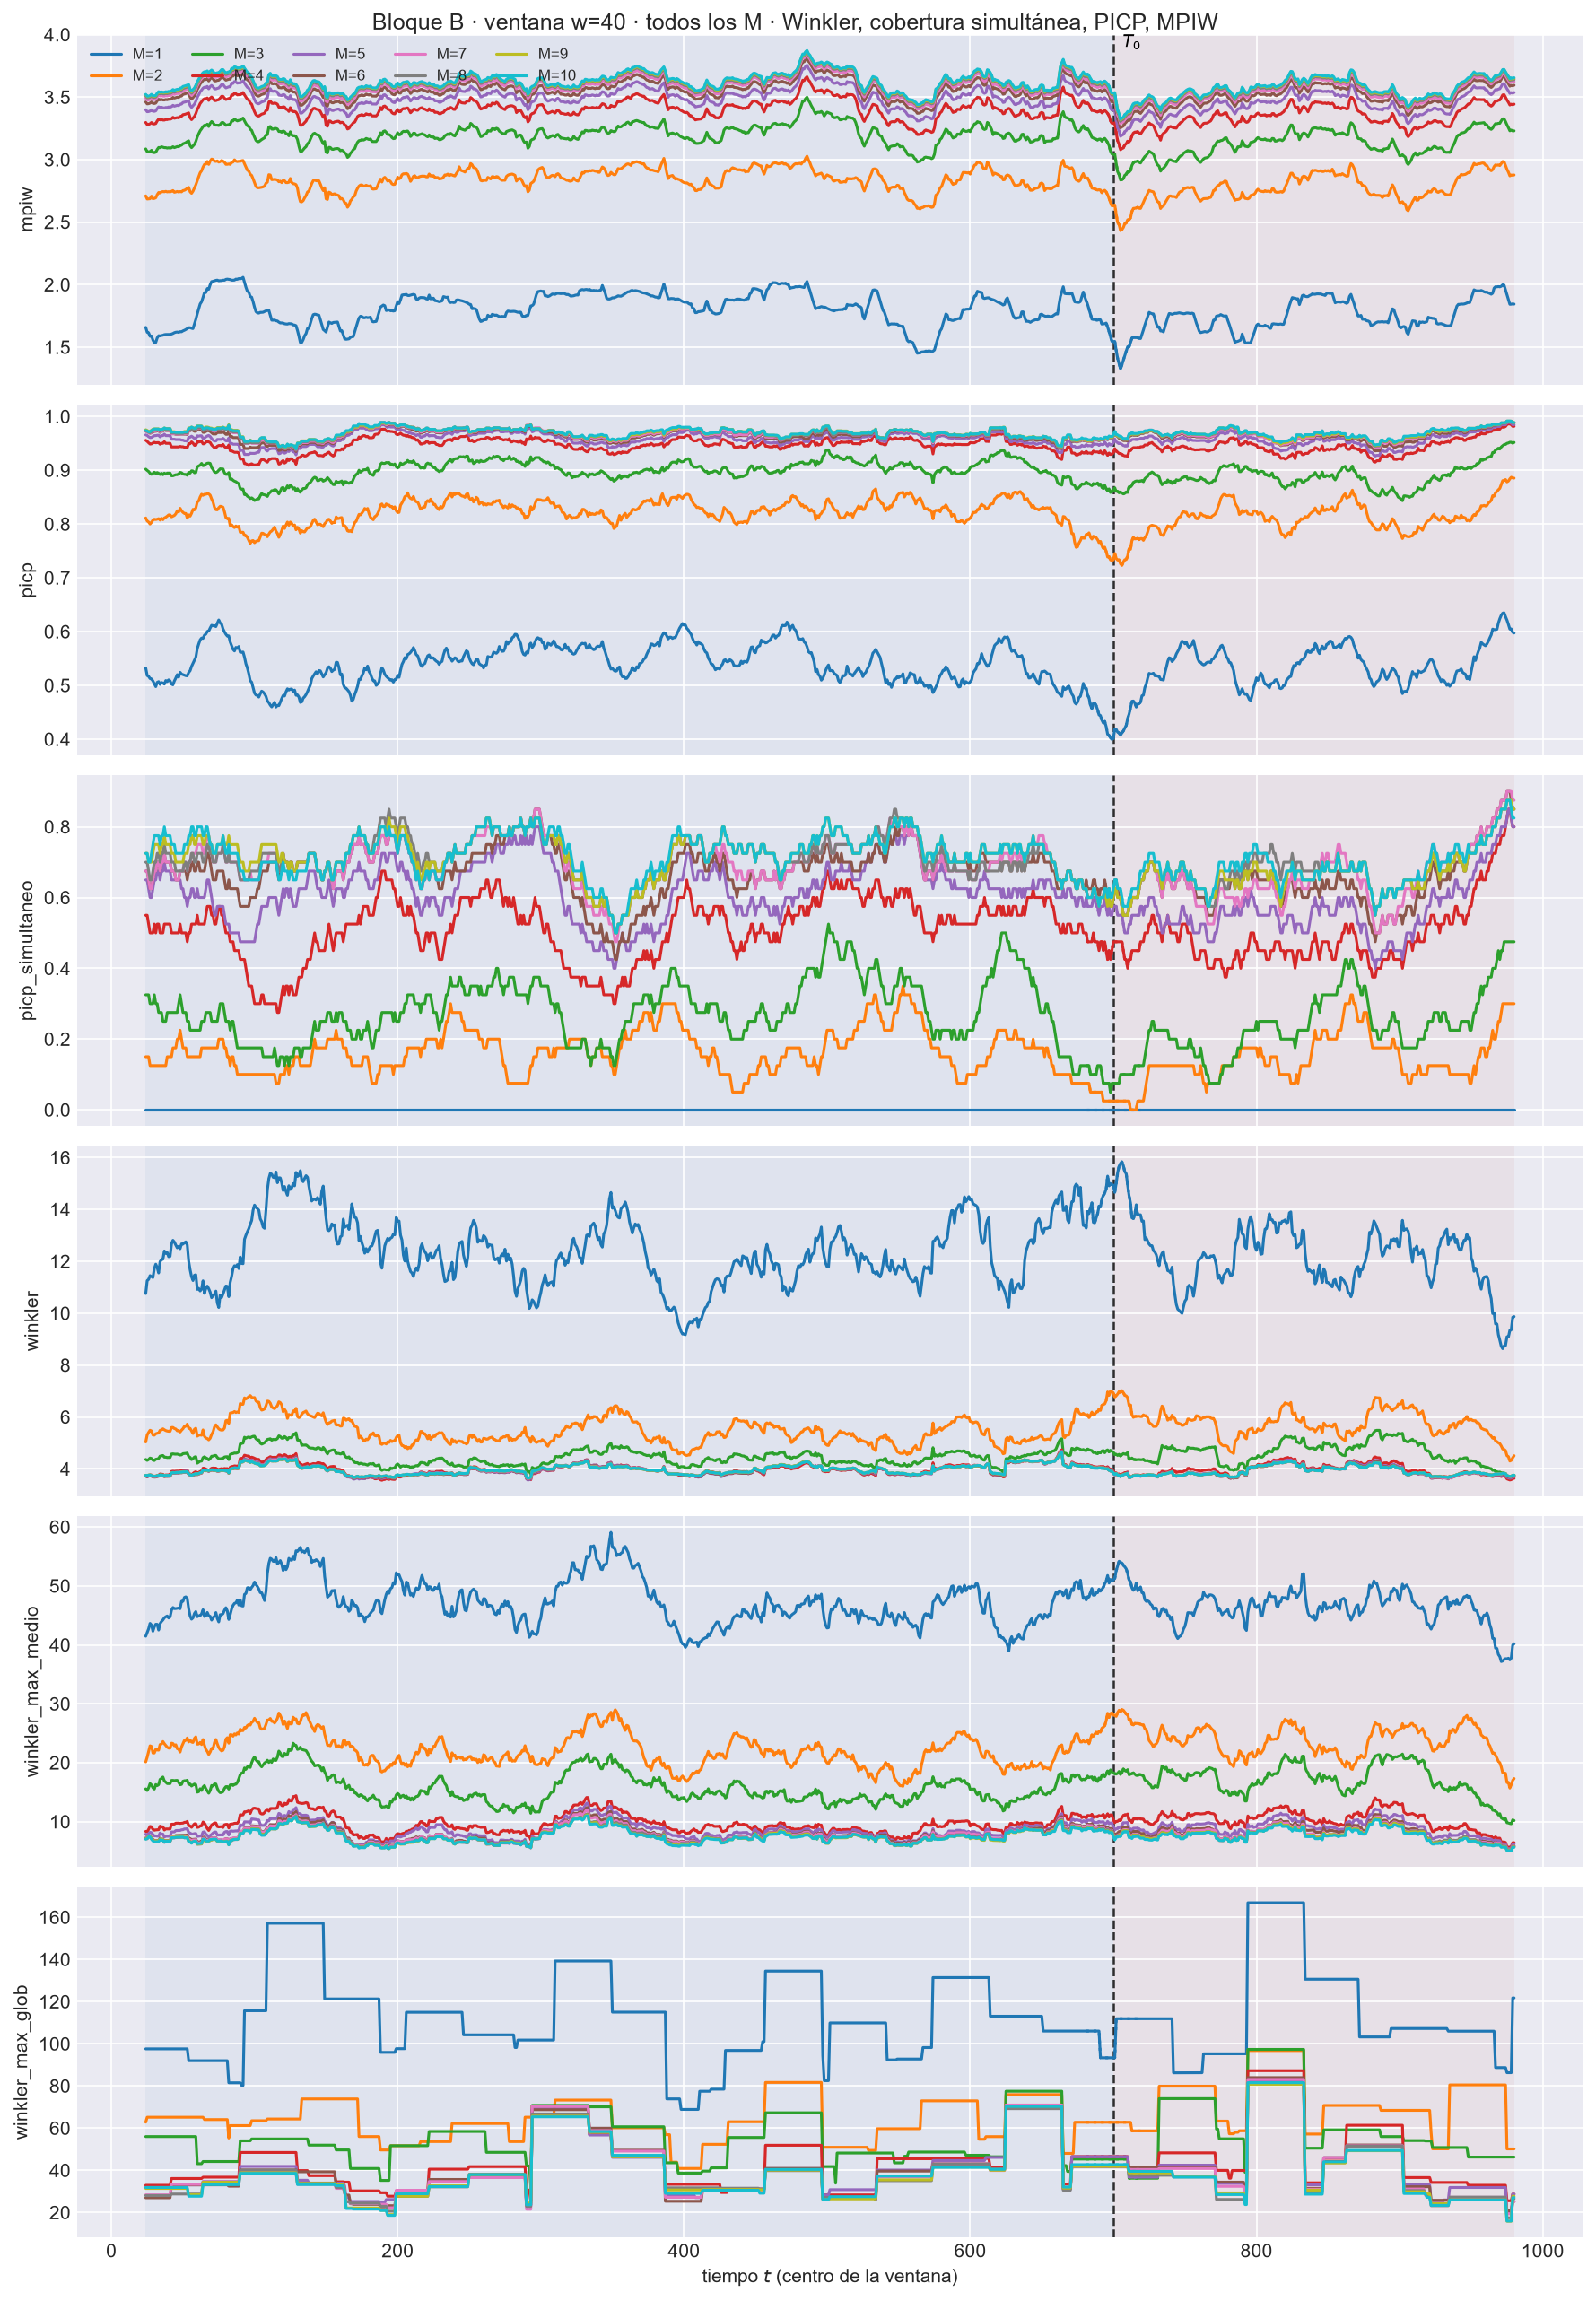
\includegraphics[width=\textwidth]{IMG/aneB_00/aneB_00_bloqueB_w40_C2.png}\end{minipage}
\caption{C-2 (TAR). Métricas de intervalo sobre la ventana móvil con $w = 20$ (izquierda) y $w = 40$ (derecha).}
\label{fig:aneB_ancho_B_C2}
\end{figure}

\begin{figure}[H]
\centering
\begin{minipage}{0.49\textwidth}\centering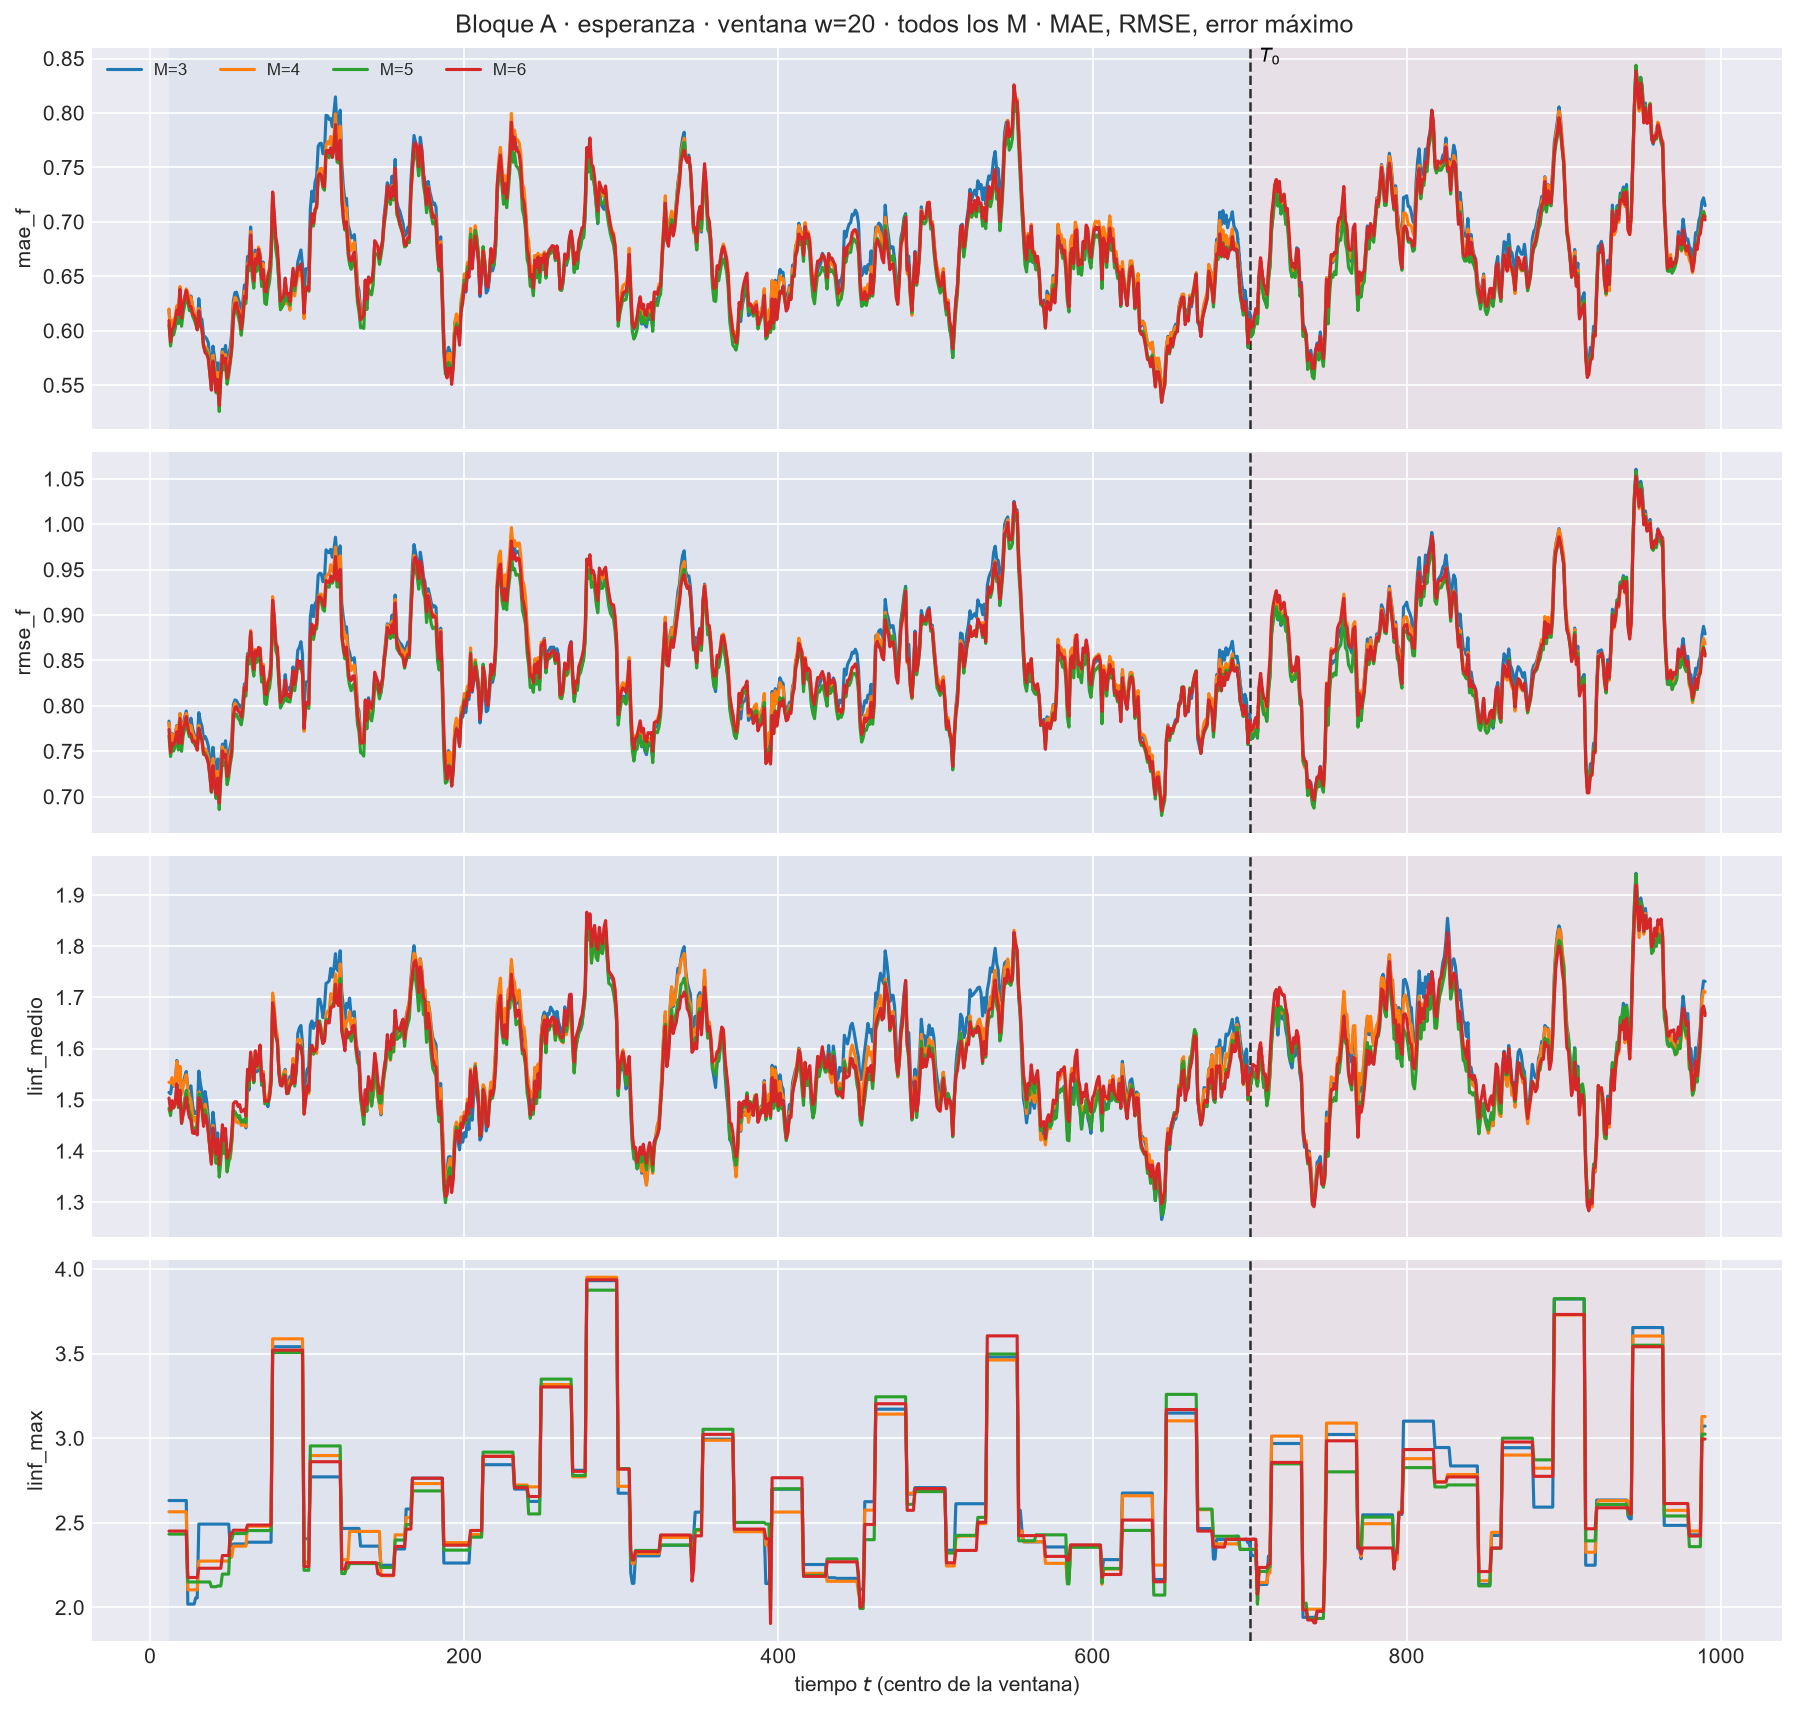
\includegraphics[width=\textwidth]{IMG/aneB_00/aneB_00_bloqueA_w20_C3.png}\end{minipage}\hfill
\begin{minipage}{0.49\textwidth}\centering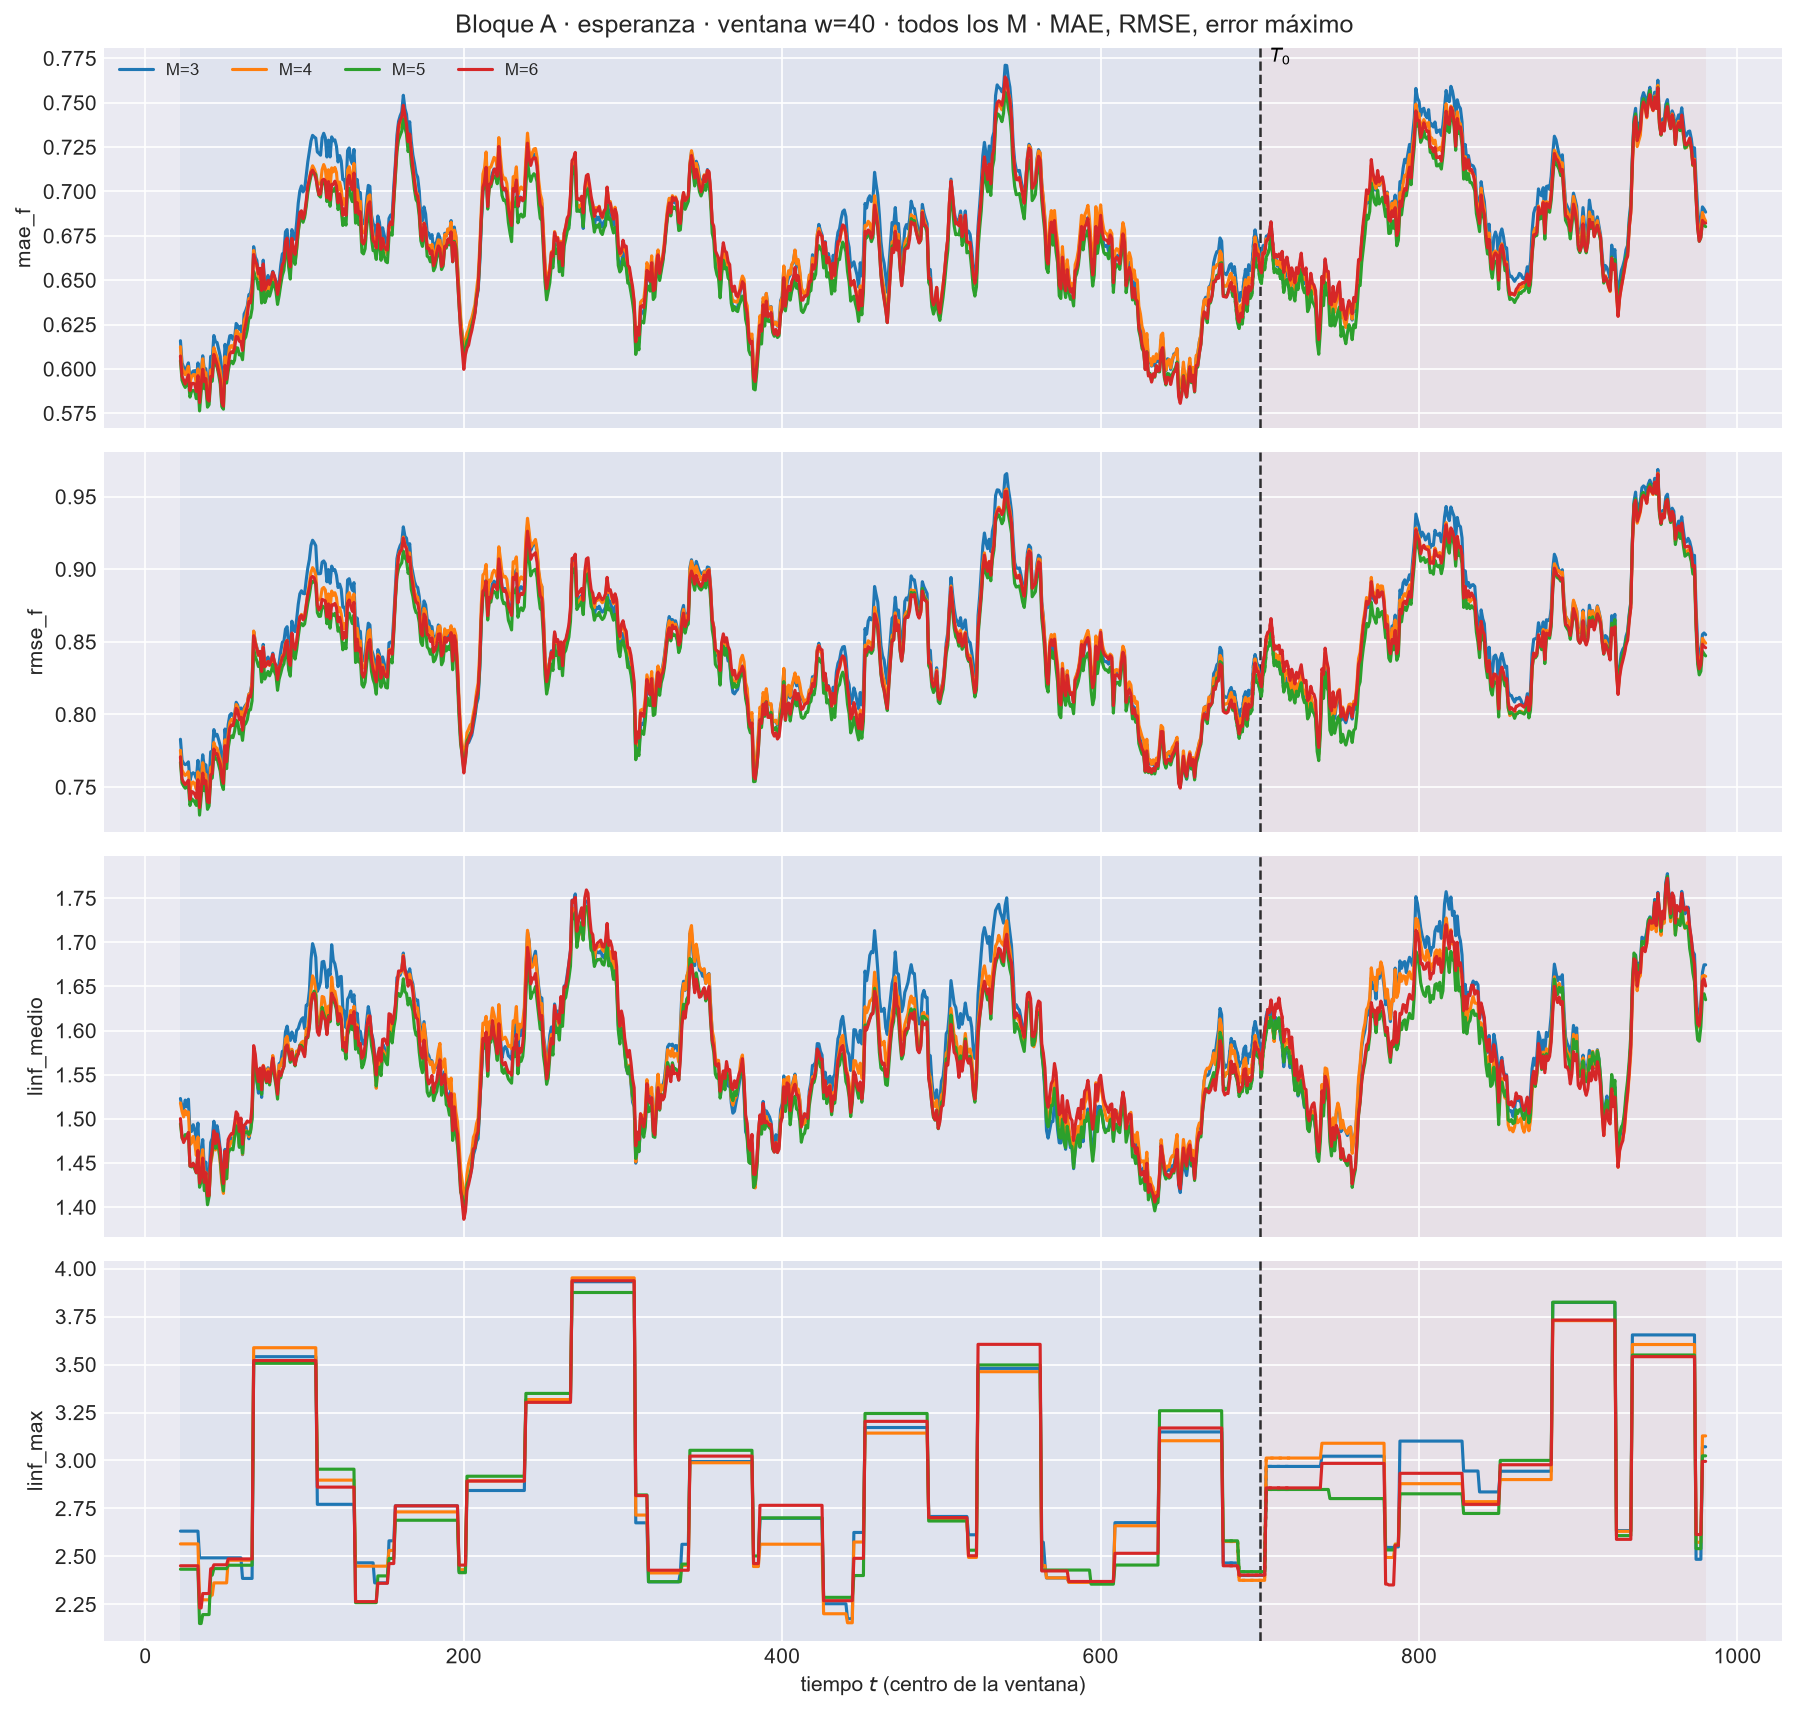
\includegraphics[width=\textwidth]{IMG/aneB_00/aneB_00_bloqueA_w40_C3.png}\end{minipage}
\caption{C-3 (multimodalidad). Métricas de error sobre la ventana móvil con $w = 20$ (izquierda) y $w = 40$ (derecha).}
\label{fig:aneB_ancho_A_C3}
\end{figure}

\begin{figure}[H]
\centering
\begin{minipage}{0.49\textwidth}\centering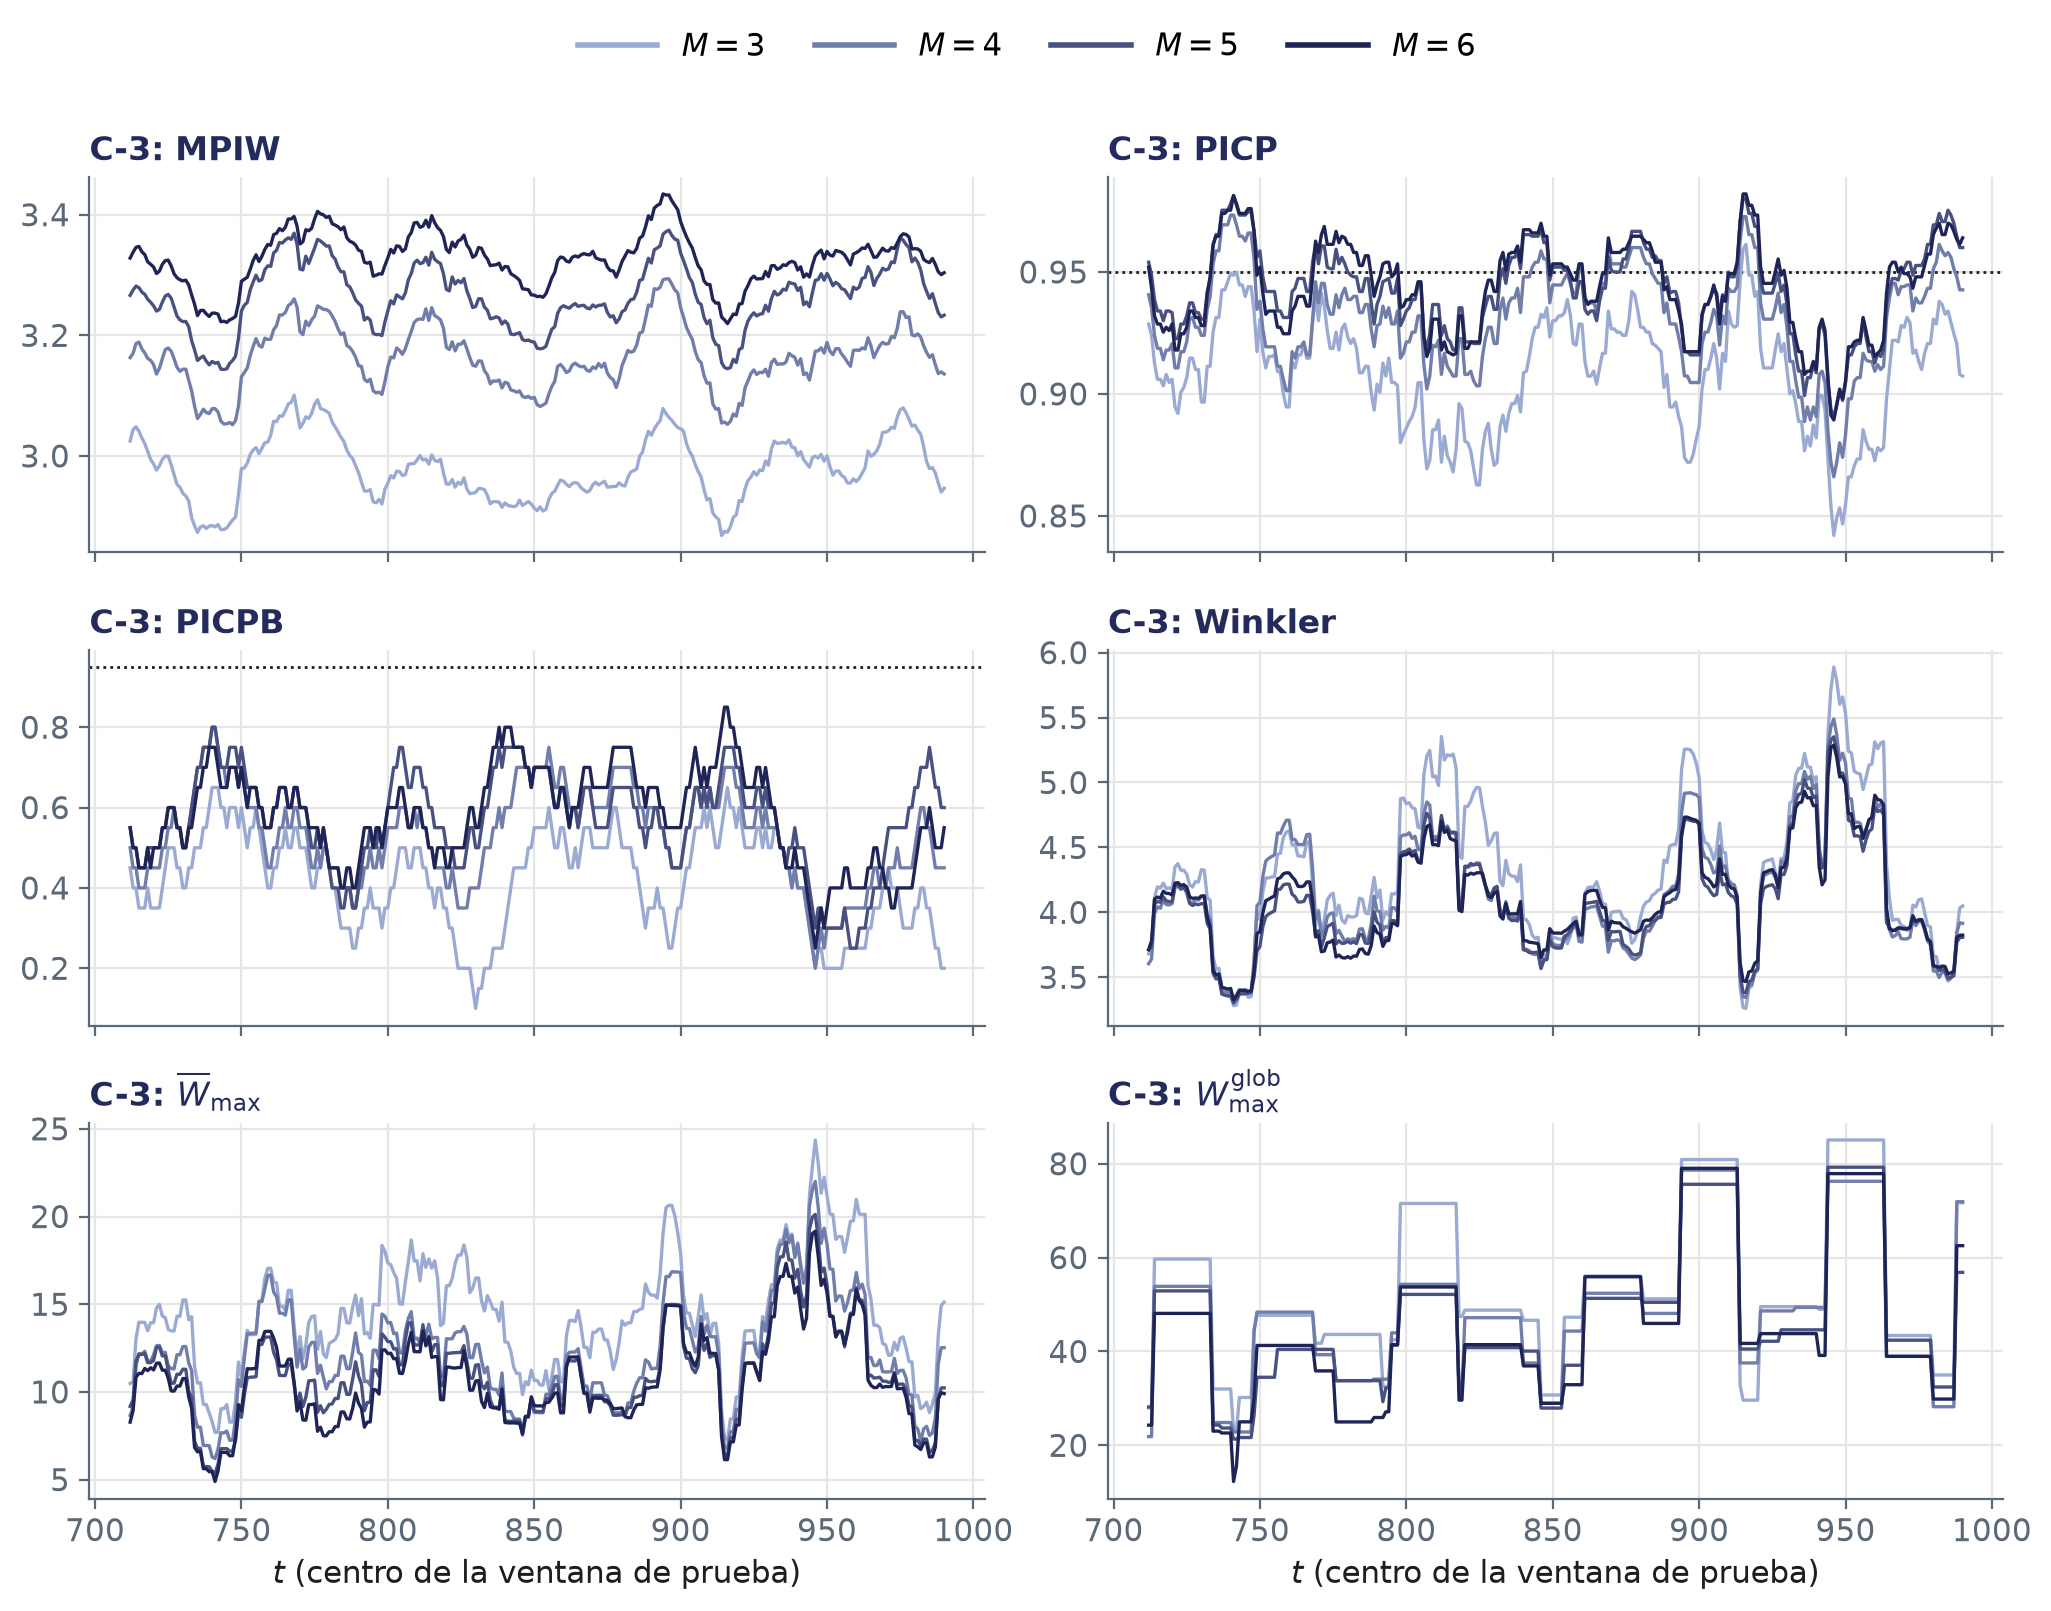
\includegraphics[width=\textwidth]{IMG/aneB_00/aneB_00_bloqueB_w20_C3.png}\end{minipage}\hfill
\begin{minipage}{0.49\textwidth}\centering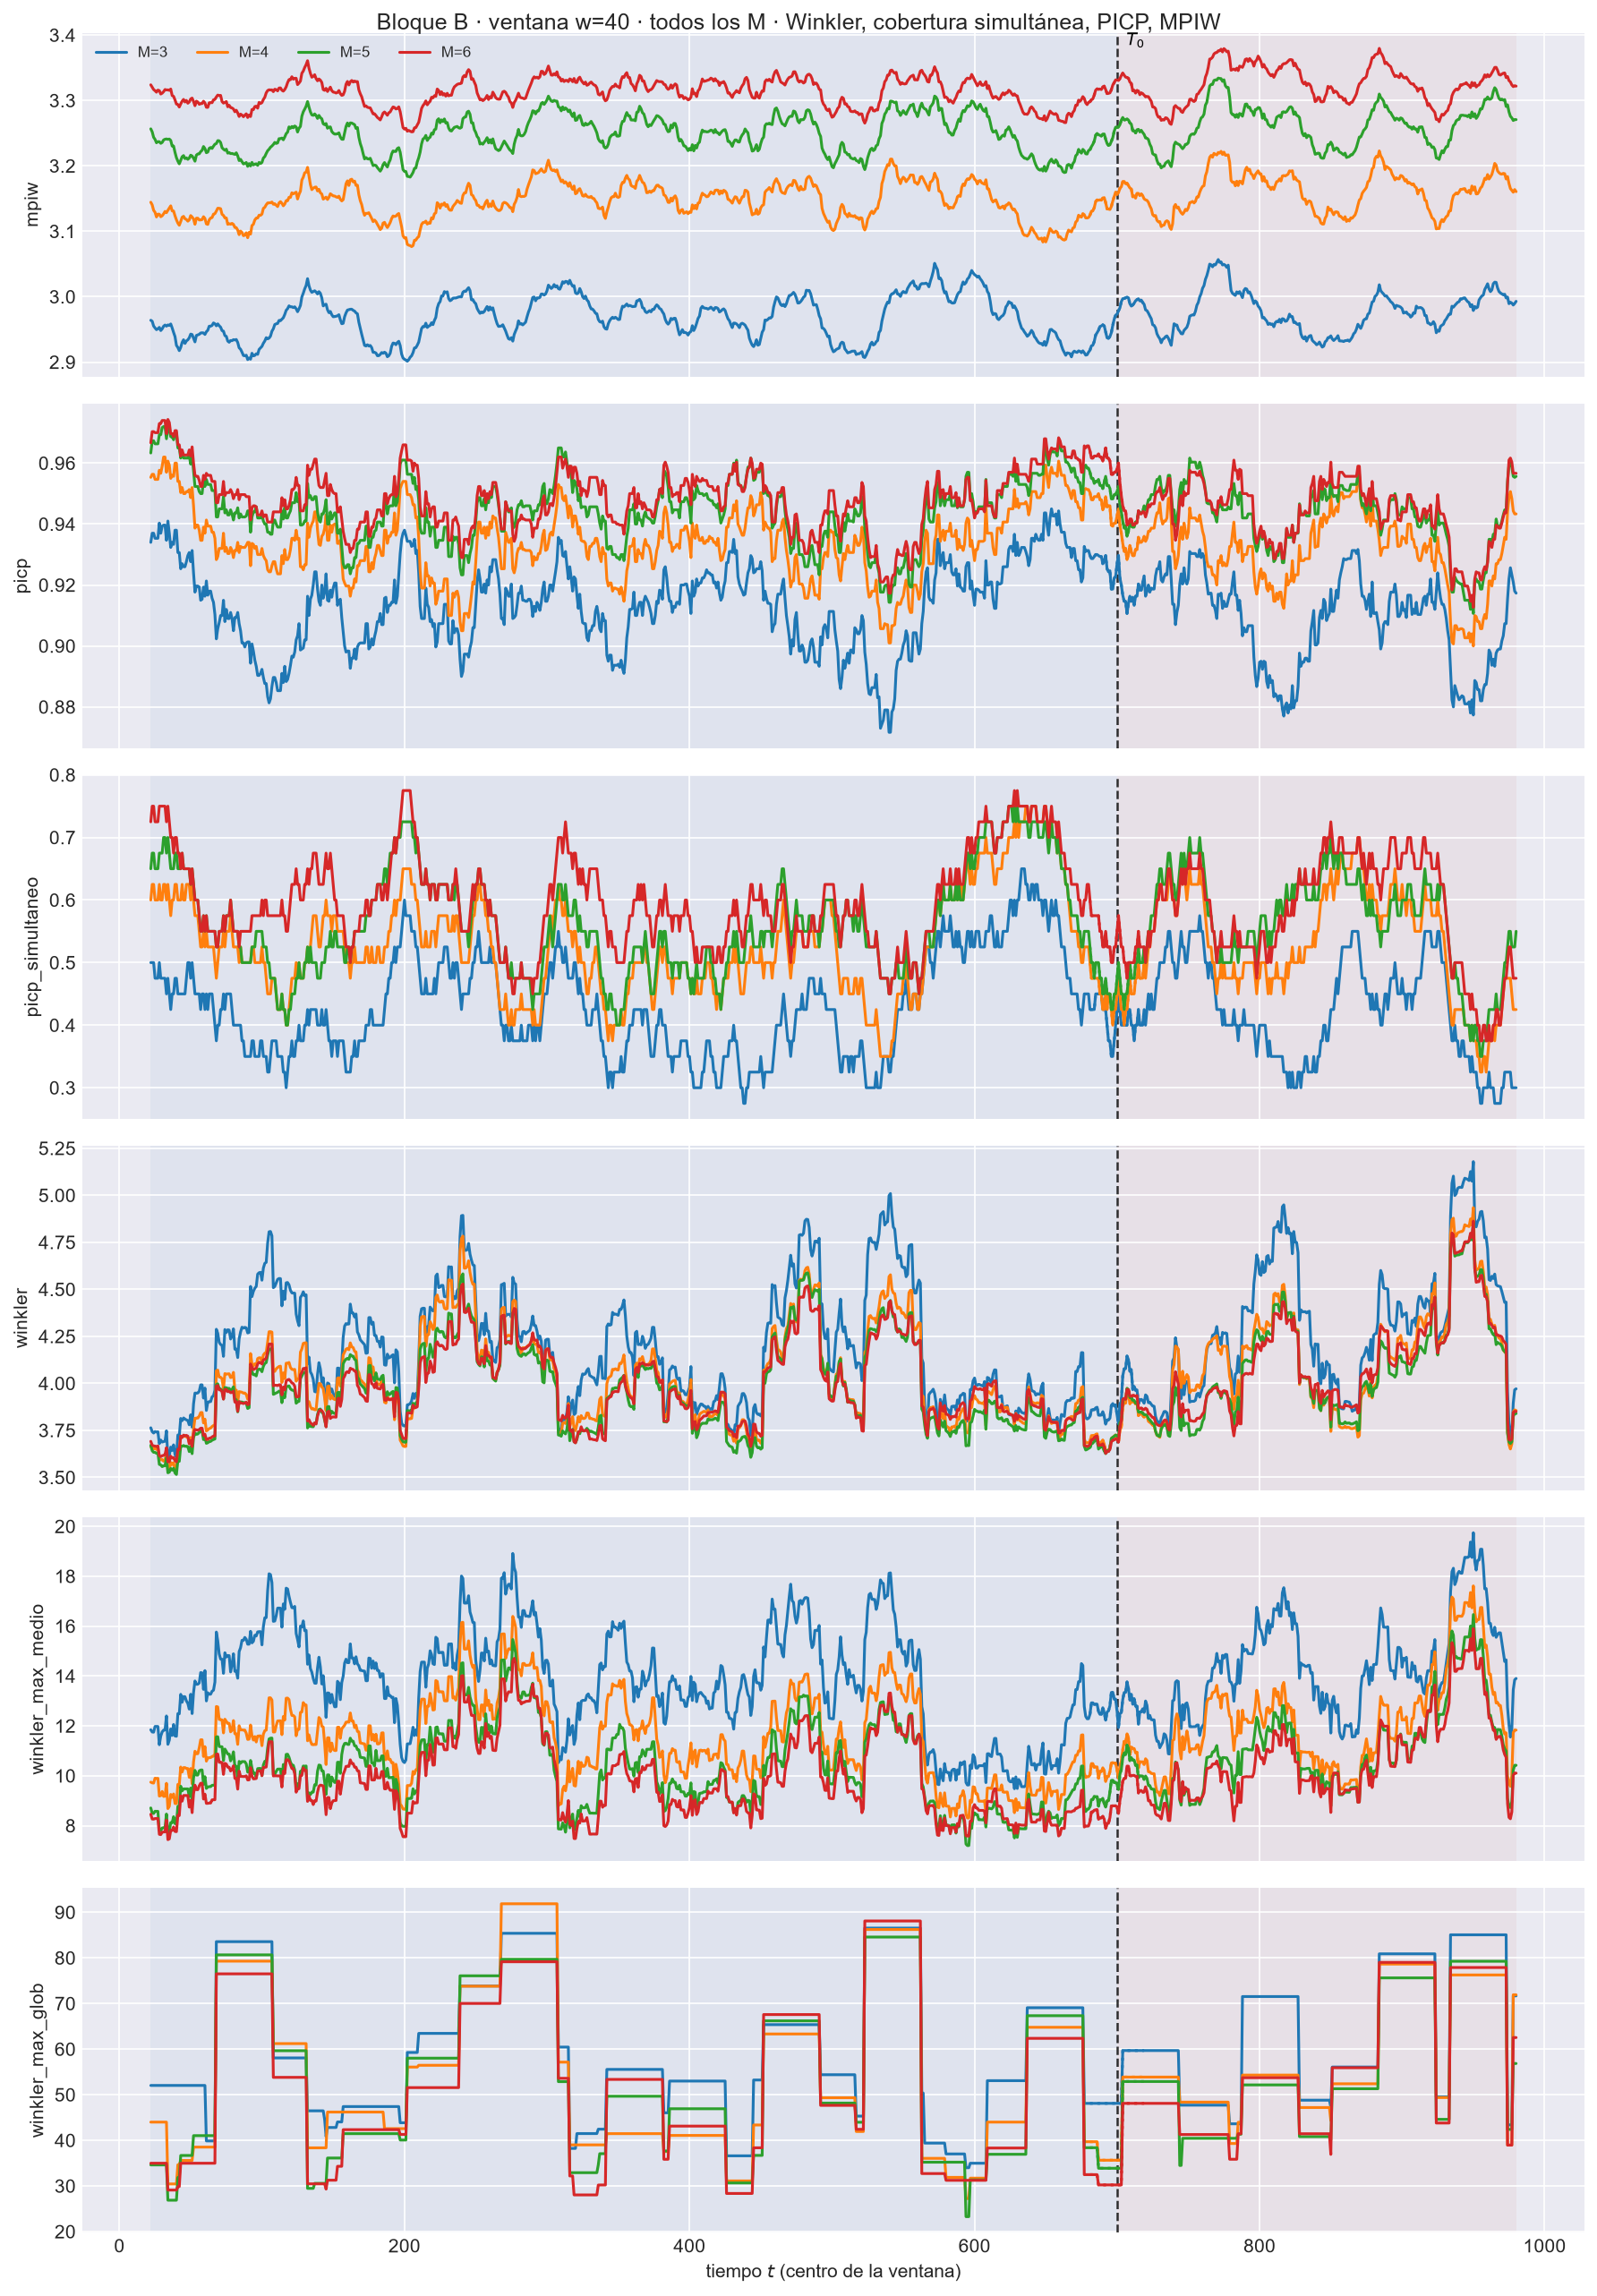
\includegraphics[width=\textwidth]{IMG/aneB_00/aneB_00_bloqueB_w40_C3.png}\end{minipage}
\caption{C-3 (multimodalidad). Métricas de intervalo sobre la ventana móvil con $w = 20$ (izquierda) y $w = 40$ (derecha).}
\label{fig:aneB_ancho_B_C3}
\end{figure}

\section{Desempeño a lo largo del período de prueba}
\label{aneB_00_03_desempeno_por_ventana}

\subsection{Error de predicción}
\label{aneB_00_03_01_ventana_error}

Error de la ventana móvil ($w = 30$) de los predictores puntuales del PSBPM-FD y de las referencias.

\begin{figure}[H]
\centering
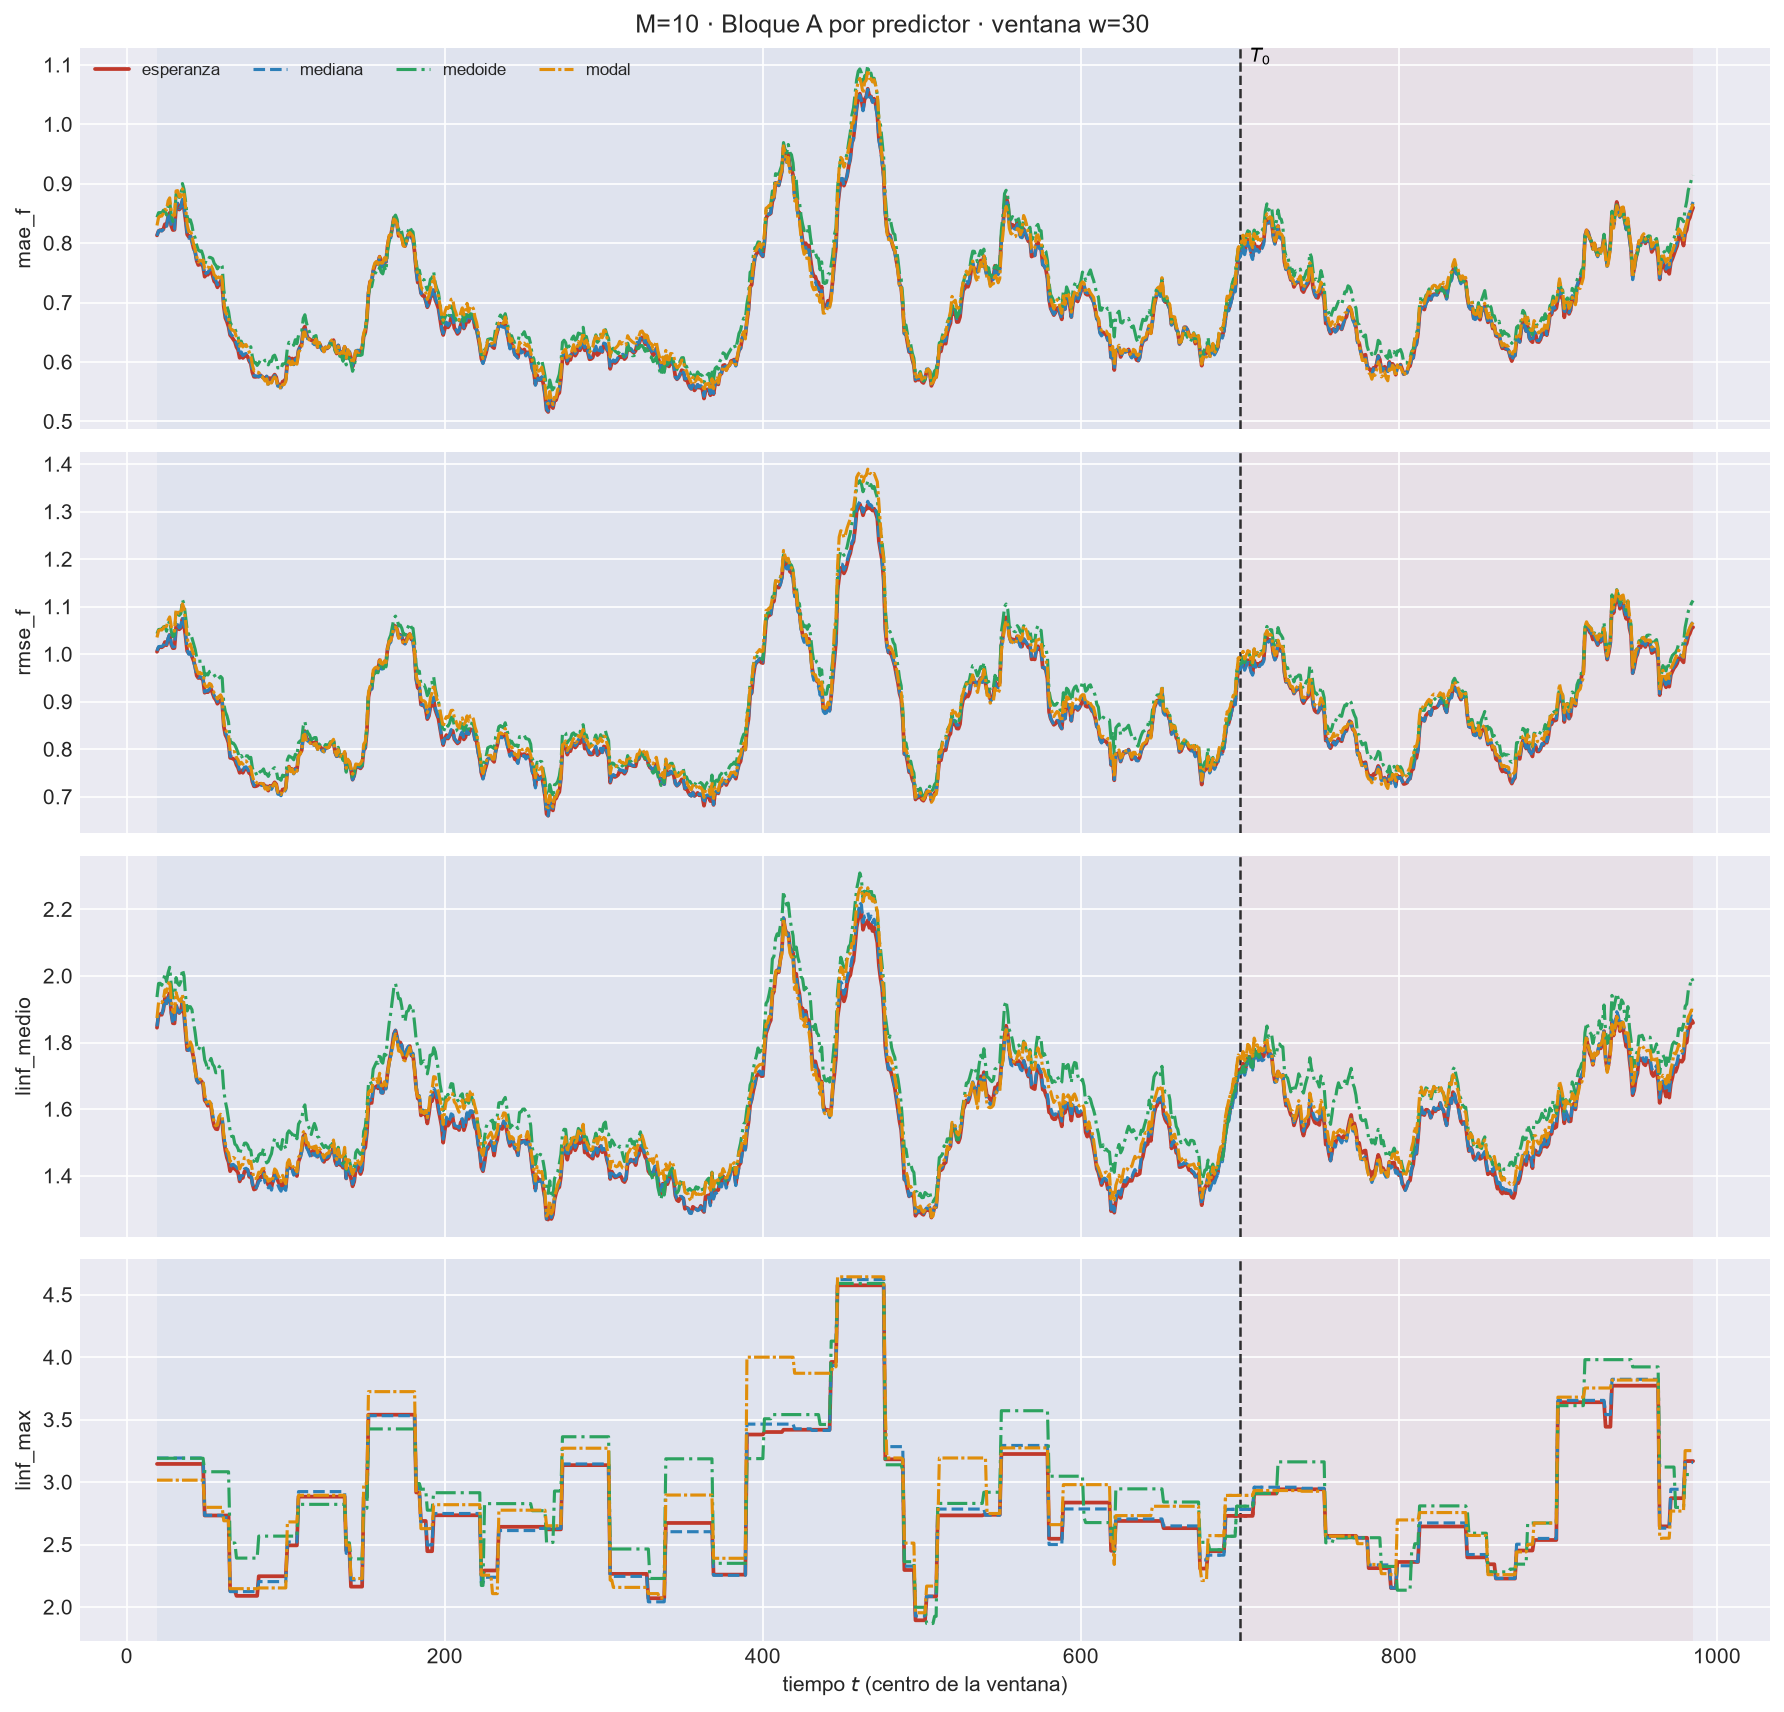
\includegraphics[width=\textwidth,height=0.8\textheight,keepaspectratio]{IMG/aneB_00/aneB_00_ventana_predictores_w30_C1.png}
\caption{C-1 (GARCH). Error de los predictores puntuales sobre la ventana móvil ($M_{\mathrm{ref}}$).}
\label{fig:aneB_pred_C1}
\end{figure}

\begin{figure}[H]
\centering
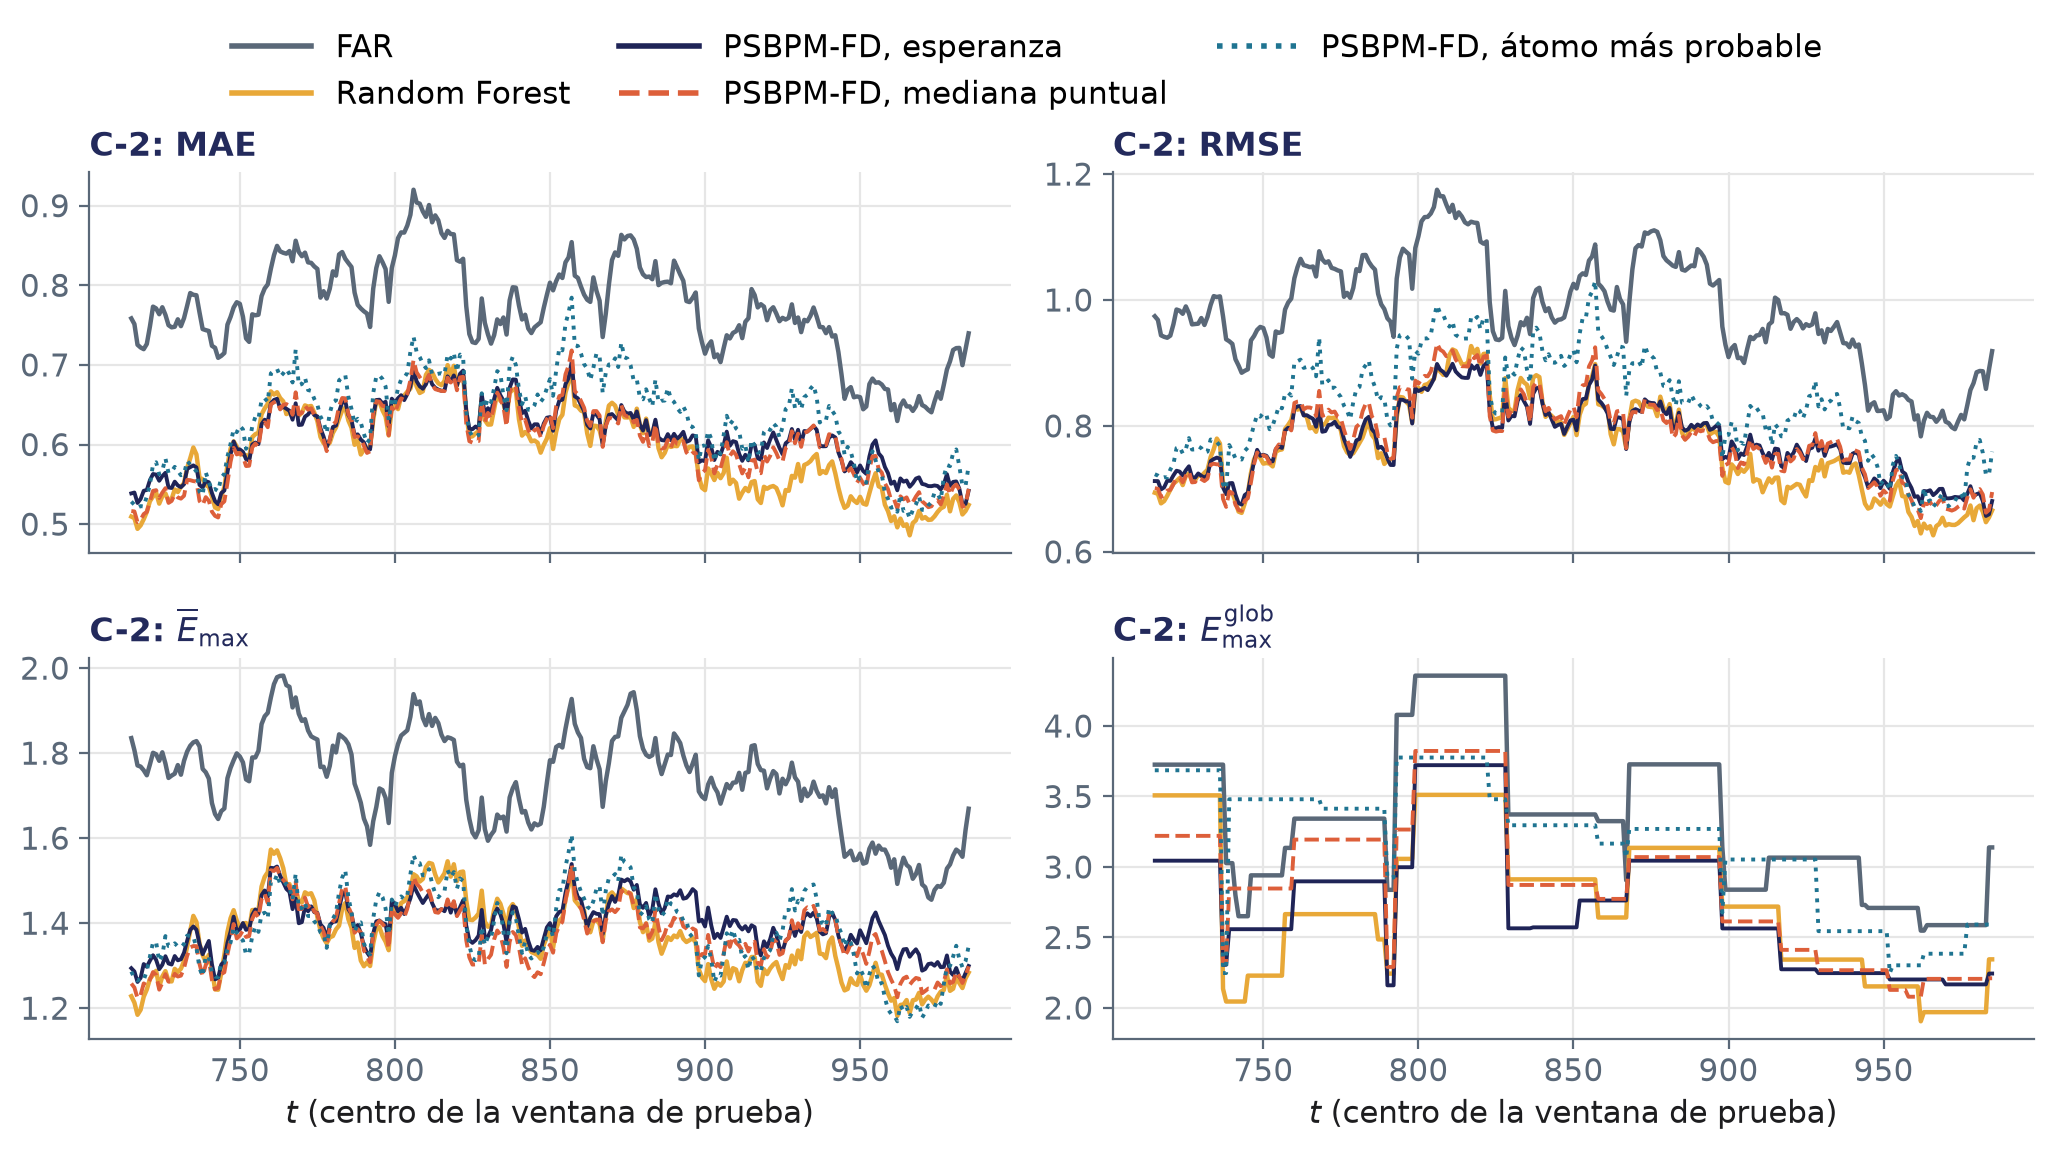
\includegraphics[width=\textwidth,height=0.8\textheight,keepaspectratio]{IMG/aneB_00/aneB_00_ventana_predictores_w30_C2.png}
\caption{C-2 (TAR). Error de los predictores puntuales sobre la ventana móvil ($M_{\mathrm{ref}}$).}
\label{fig:aneB_pred_C2}
\end{figure}

\begin{figure}[H]
\centering
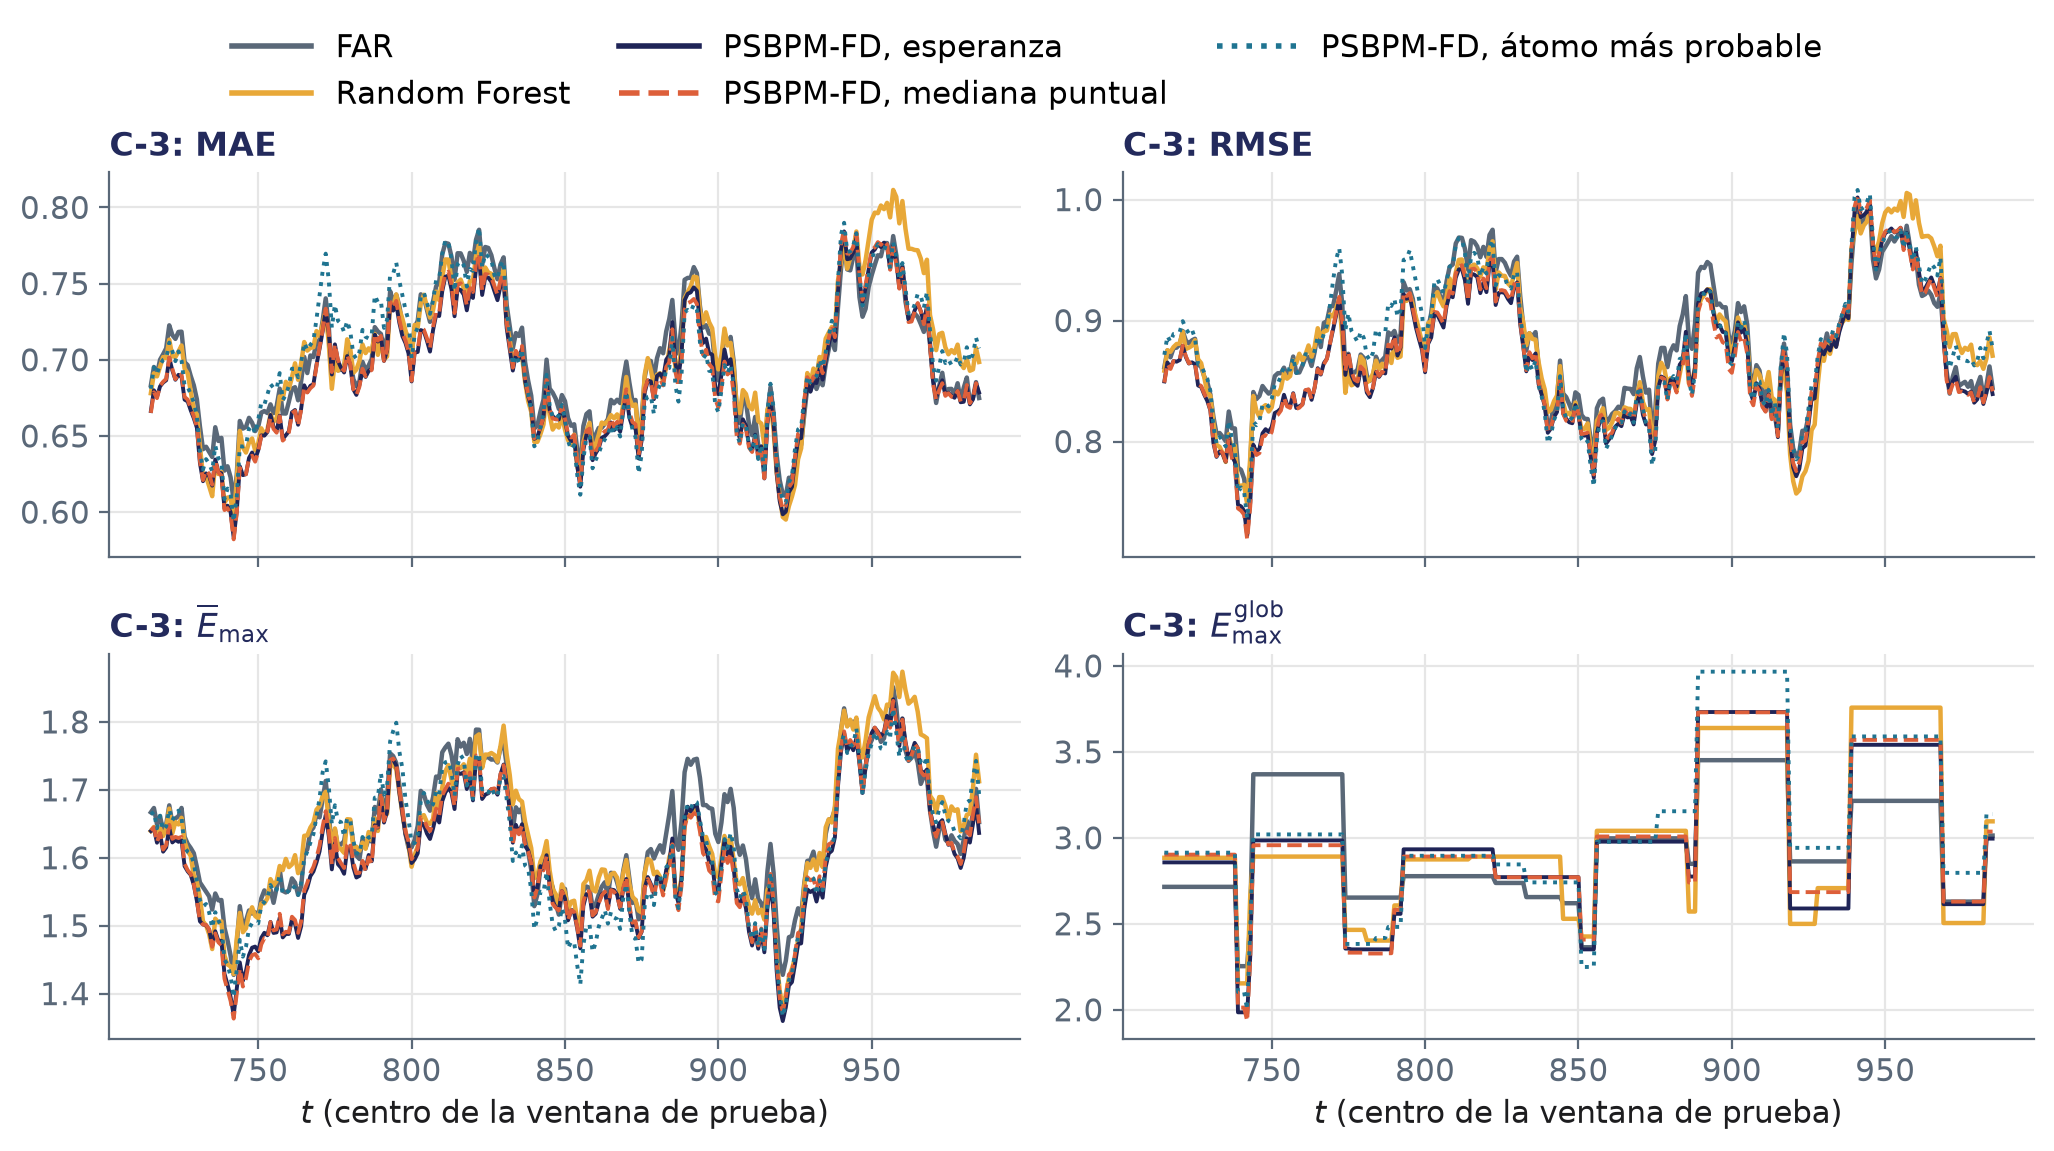
\includegraphics[width=\textwidth,height=0.8\textheight,keepaspectratio]{IMG/aneB_00/aneB_00_ventana_predictores_w30_C3.png}
\caption{C-3 (multimodalidad). Error de los predictores puntuales sobre la ventana móvil ($M_{\mathrm{ref}}$).}
\label{fig:aneB_pred_C3}
\end{figure}

\subsection{Intervalos de predicción}
\label{aneB_00_03_02_ventana_intervalos}

Métricas de intervalo de la ventana móvil ($w = 30$) de las tres construcciones del PSBPM-FD y del FAR.

\begin{figure}[H]
\centering
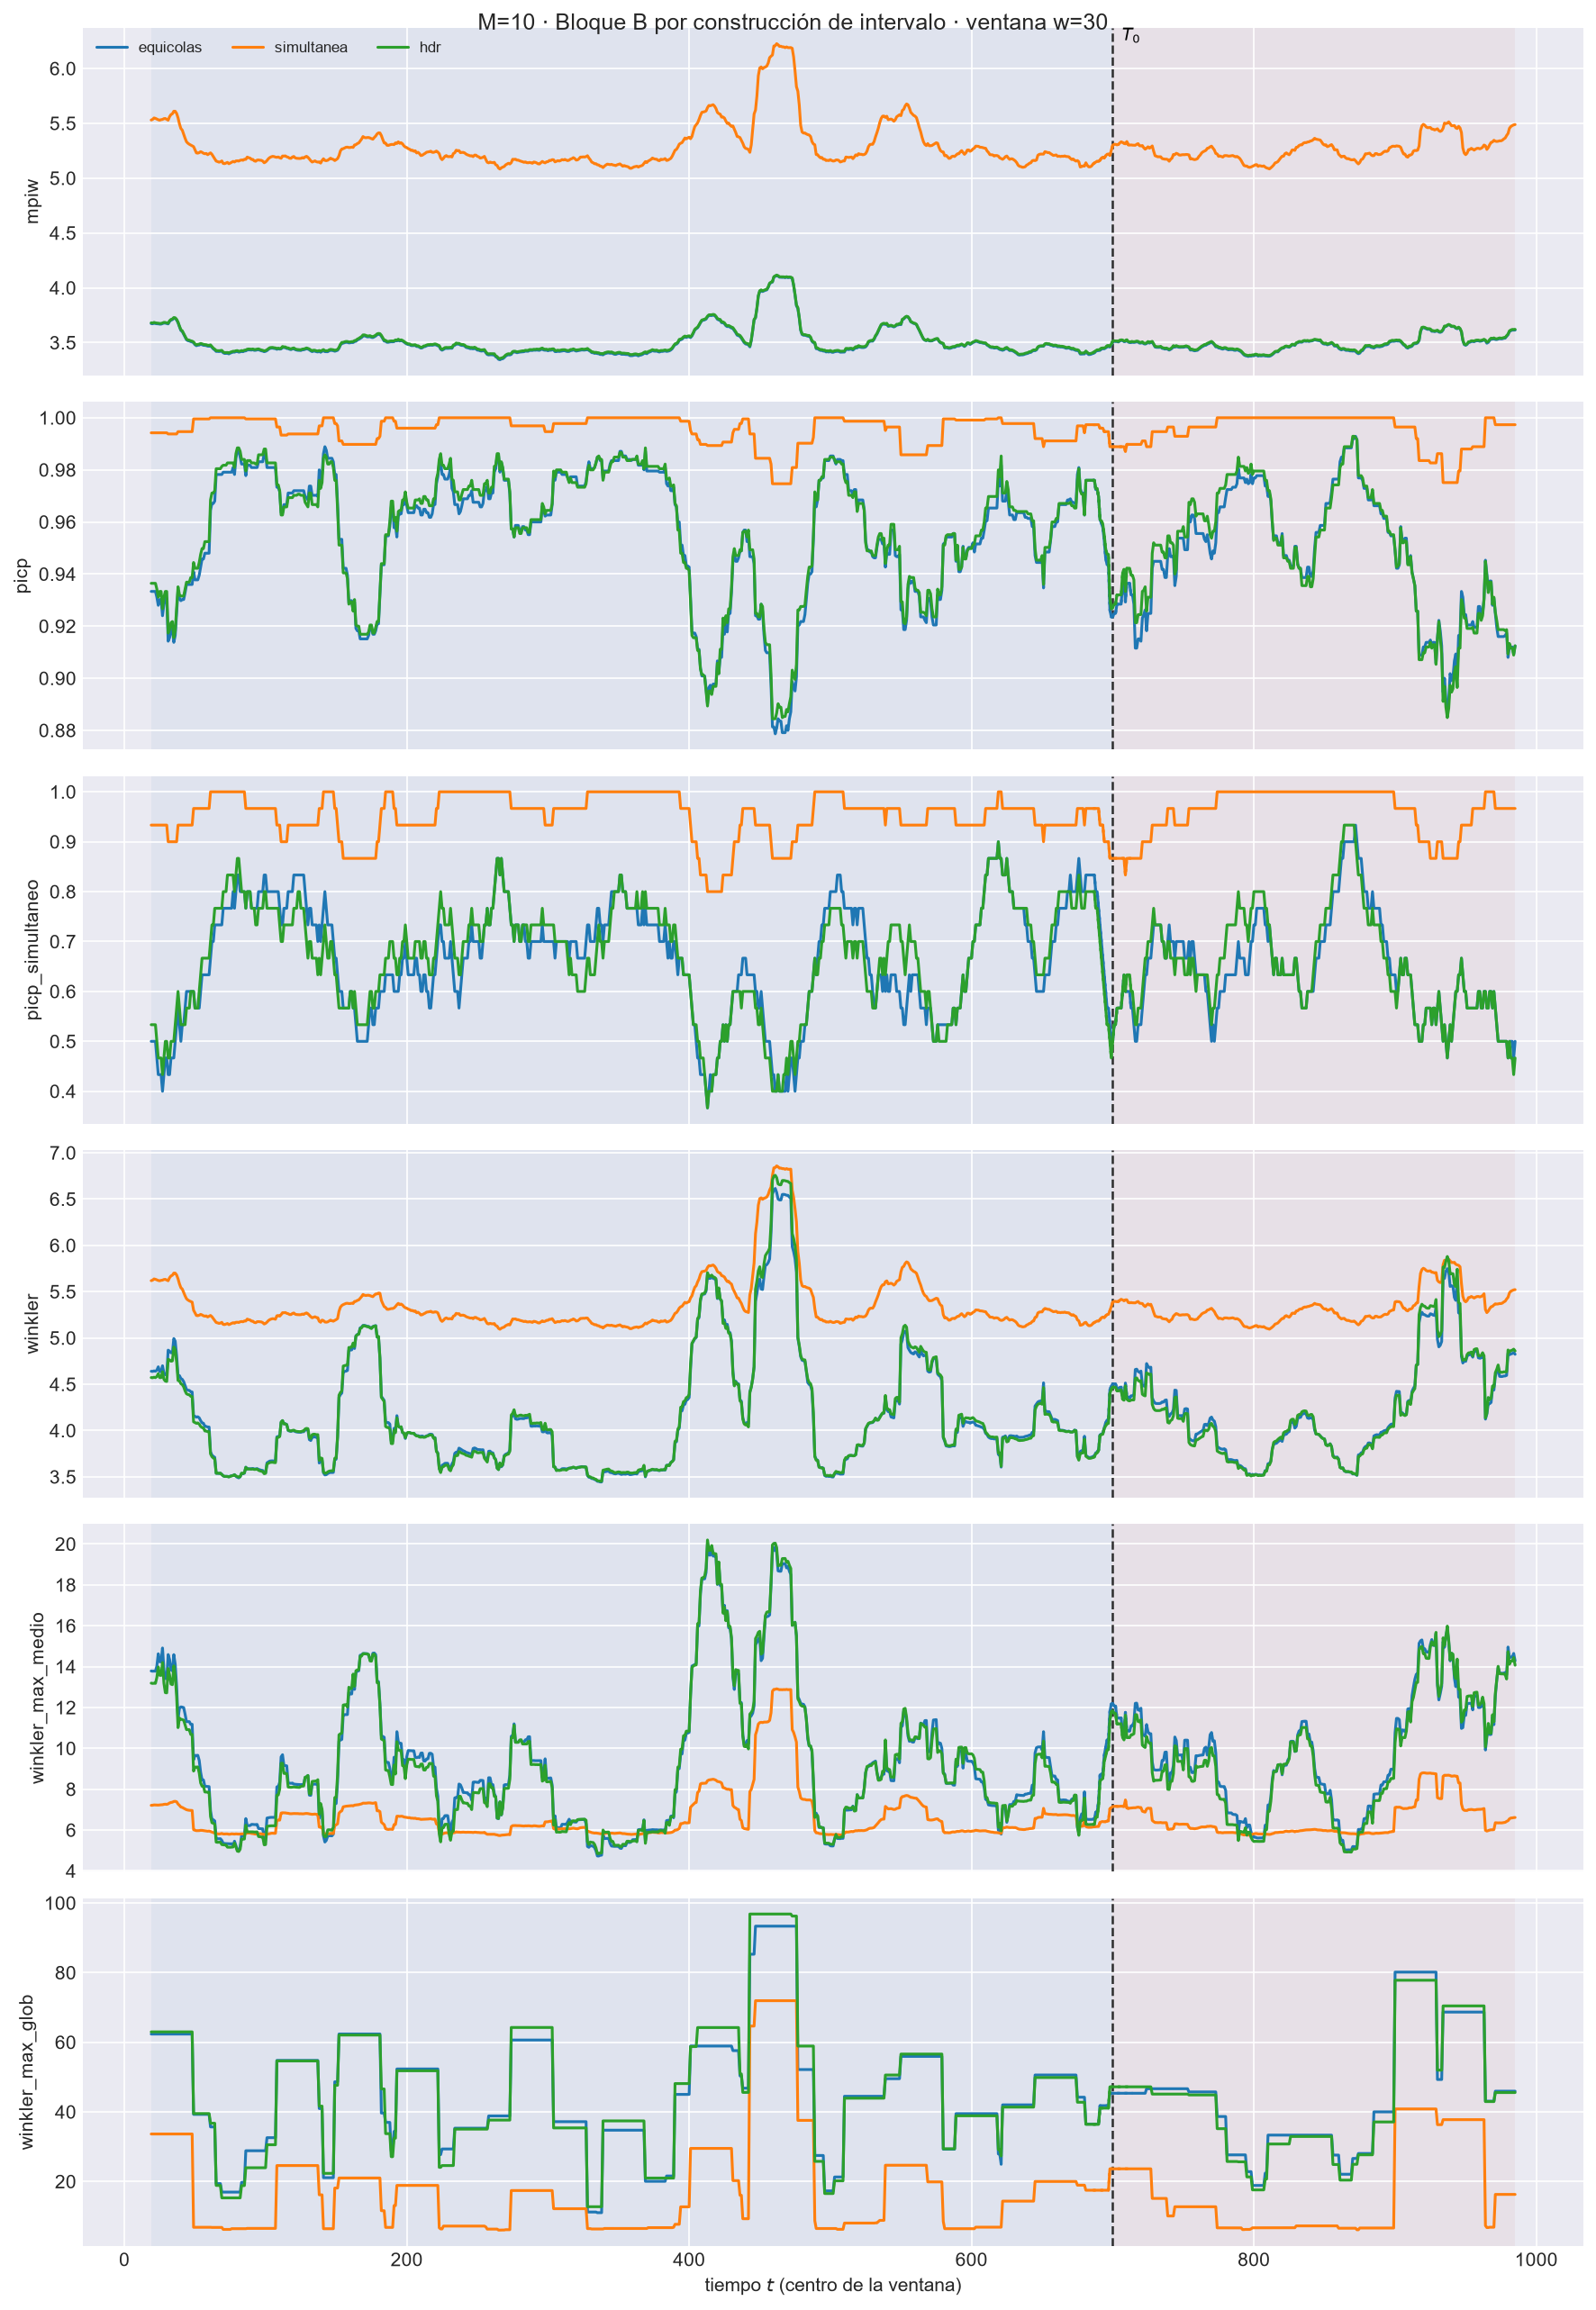
\includegraphics[width=\textwidth,height=0.75\textheight,keepaspectratio]{IMG/aneB_00/aneB_00_ventana_intervalos_w30_C1.png}
\caption{C-1 (GARCH). Métricas de intervalo sobre la ventana móvil ($M_{\mathrm{ref}}$).}
\label{fig:aneB_int_C1}
\end{figure}

\begin{figure}[H]
\centering
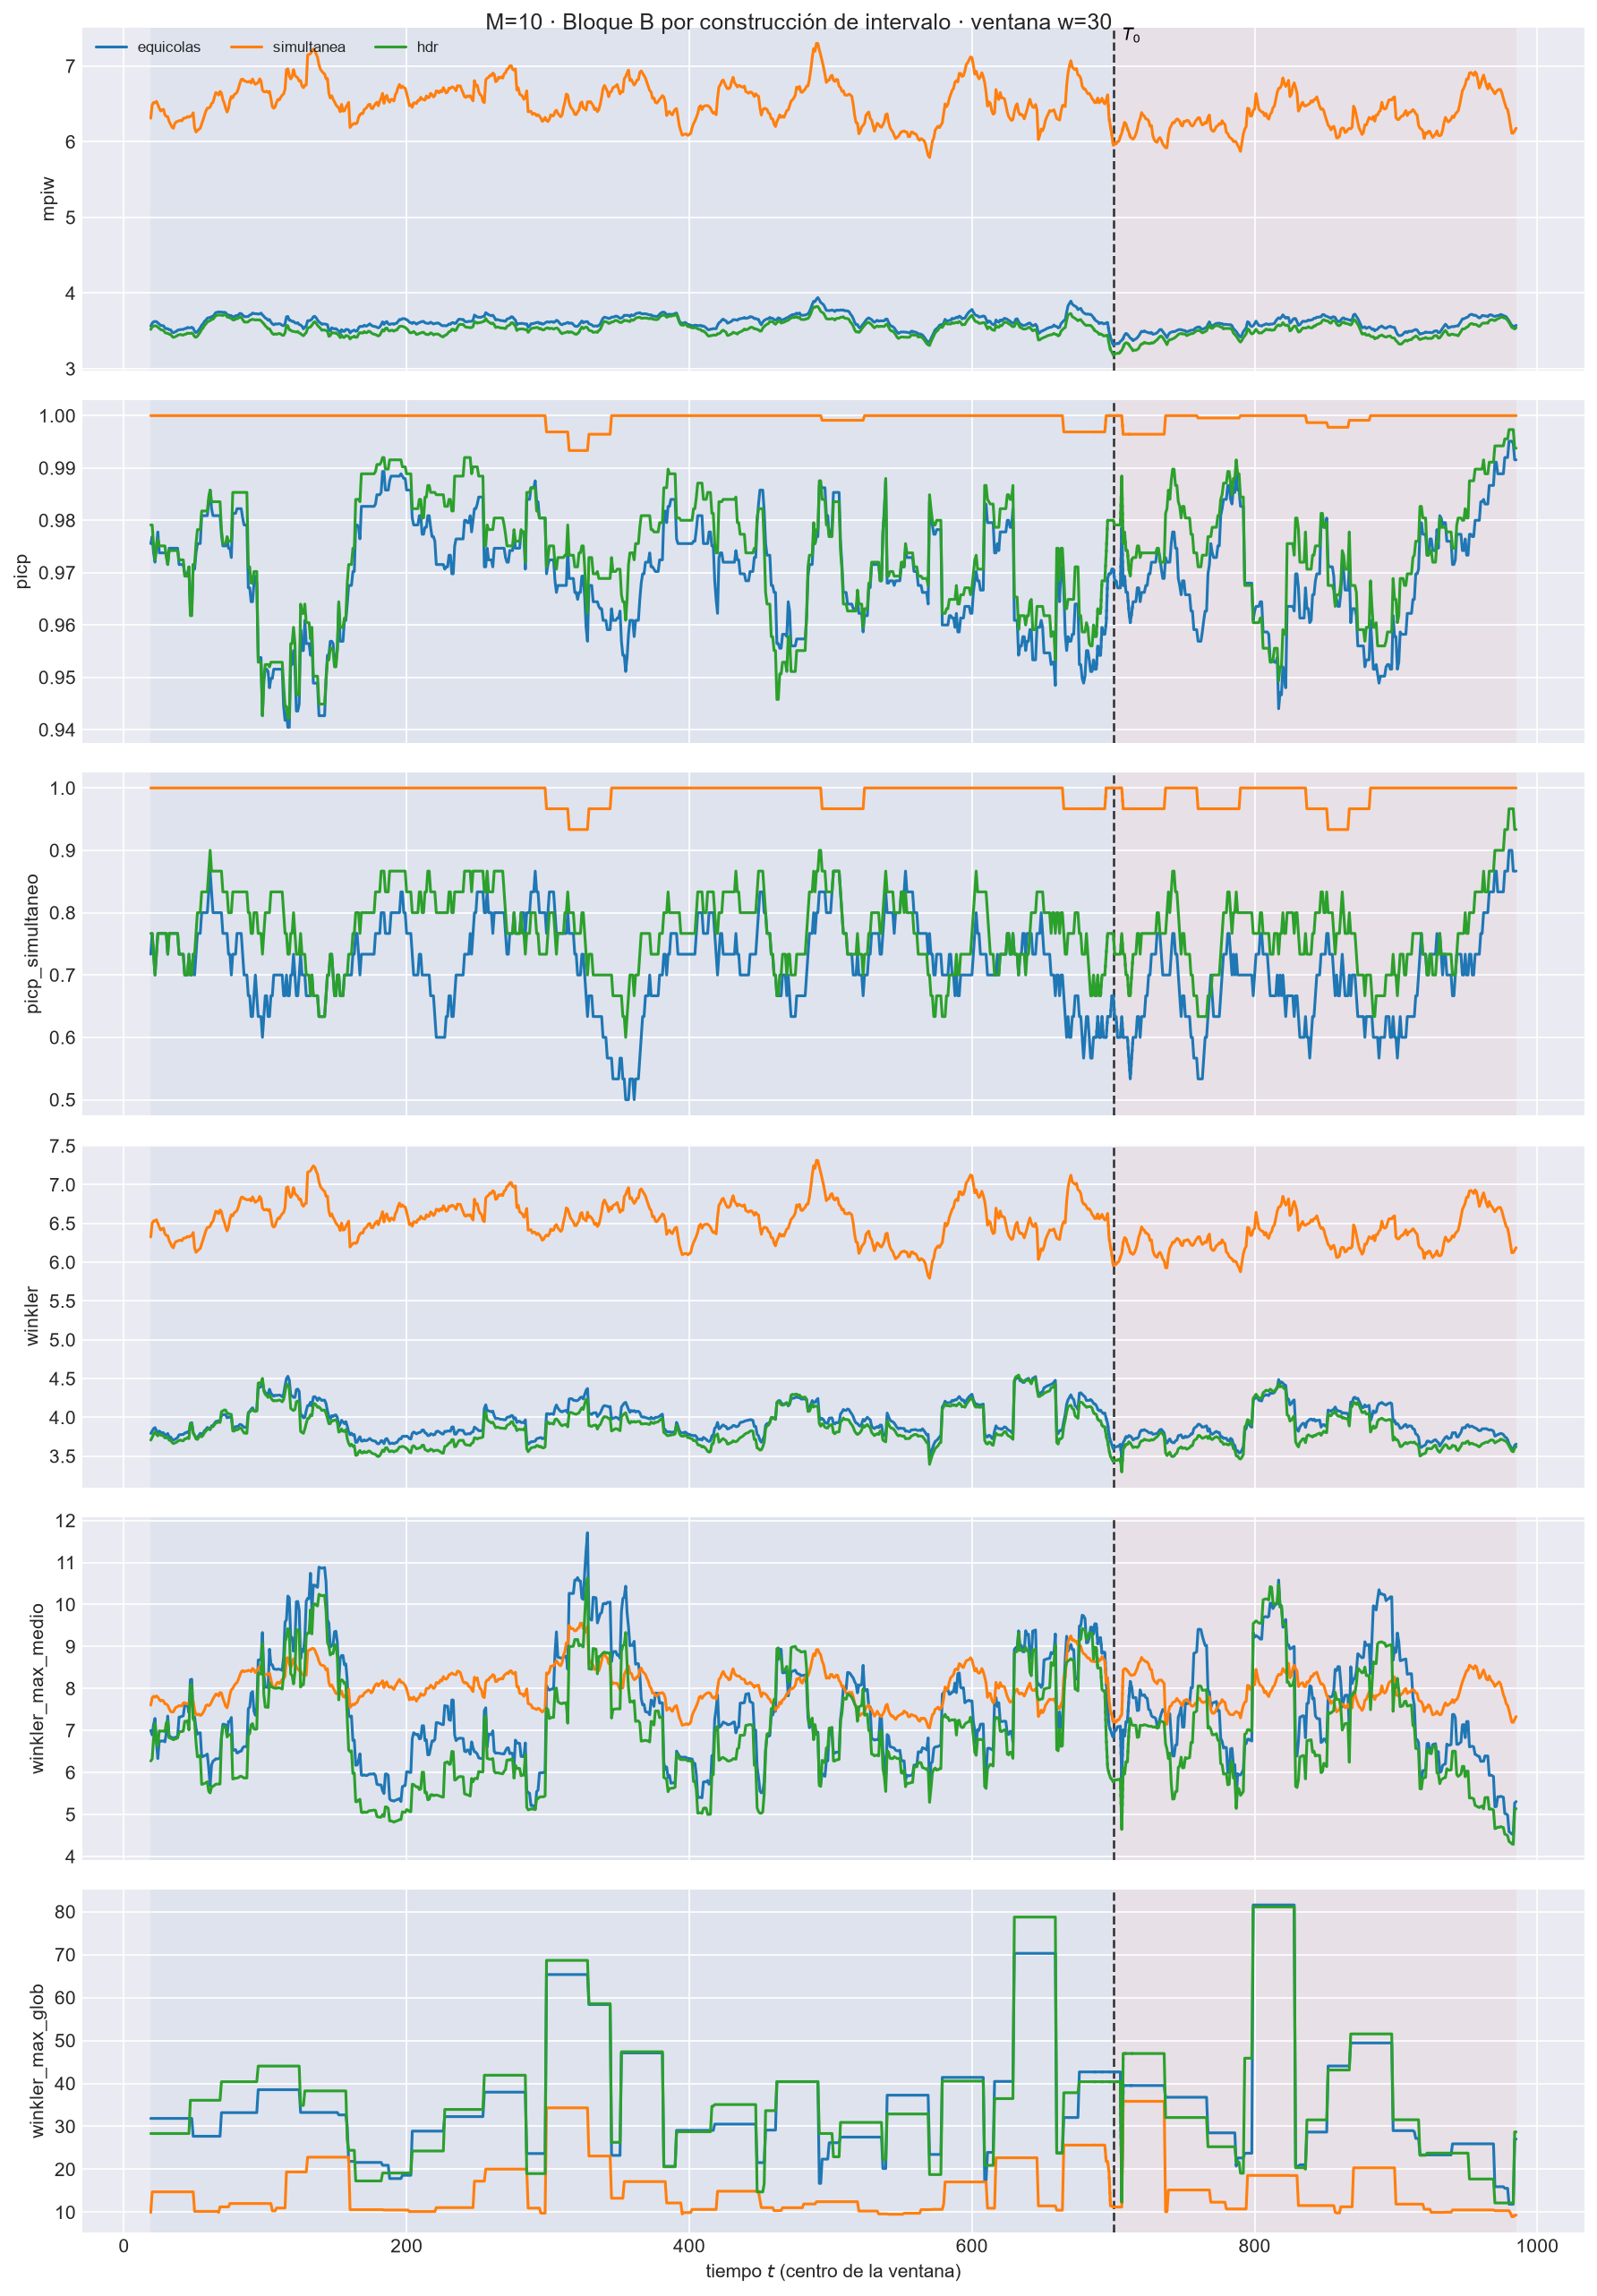
\includegraphics[width=\textwidth,height=0.75\textheight,keepaspectratio]{IMG/aneB_00/aneB_00_ventana_intervalos_w30_C2.png}
\caption{C-2 (TAR). Métricas de intervalo sobre la ventana móvil ($M_{\mathrm{ref}}$).}
\label{fig:aneB_int_C2}
\end{figure}

\begin{figure}[H]
\centering
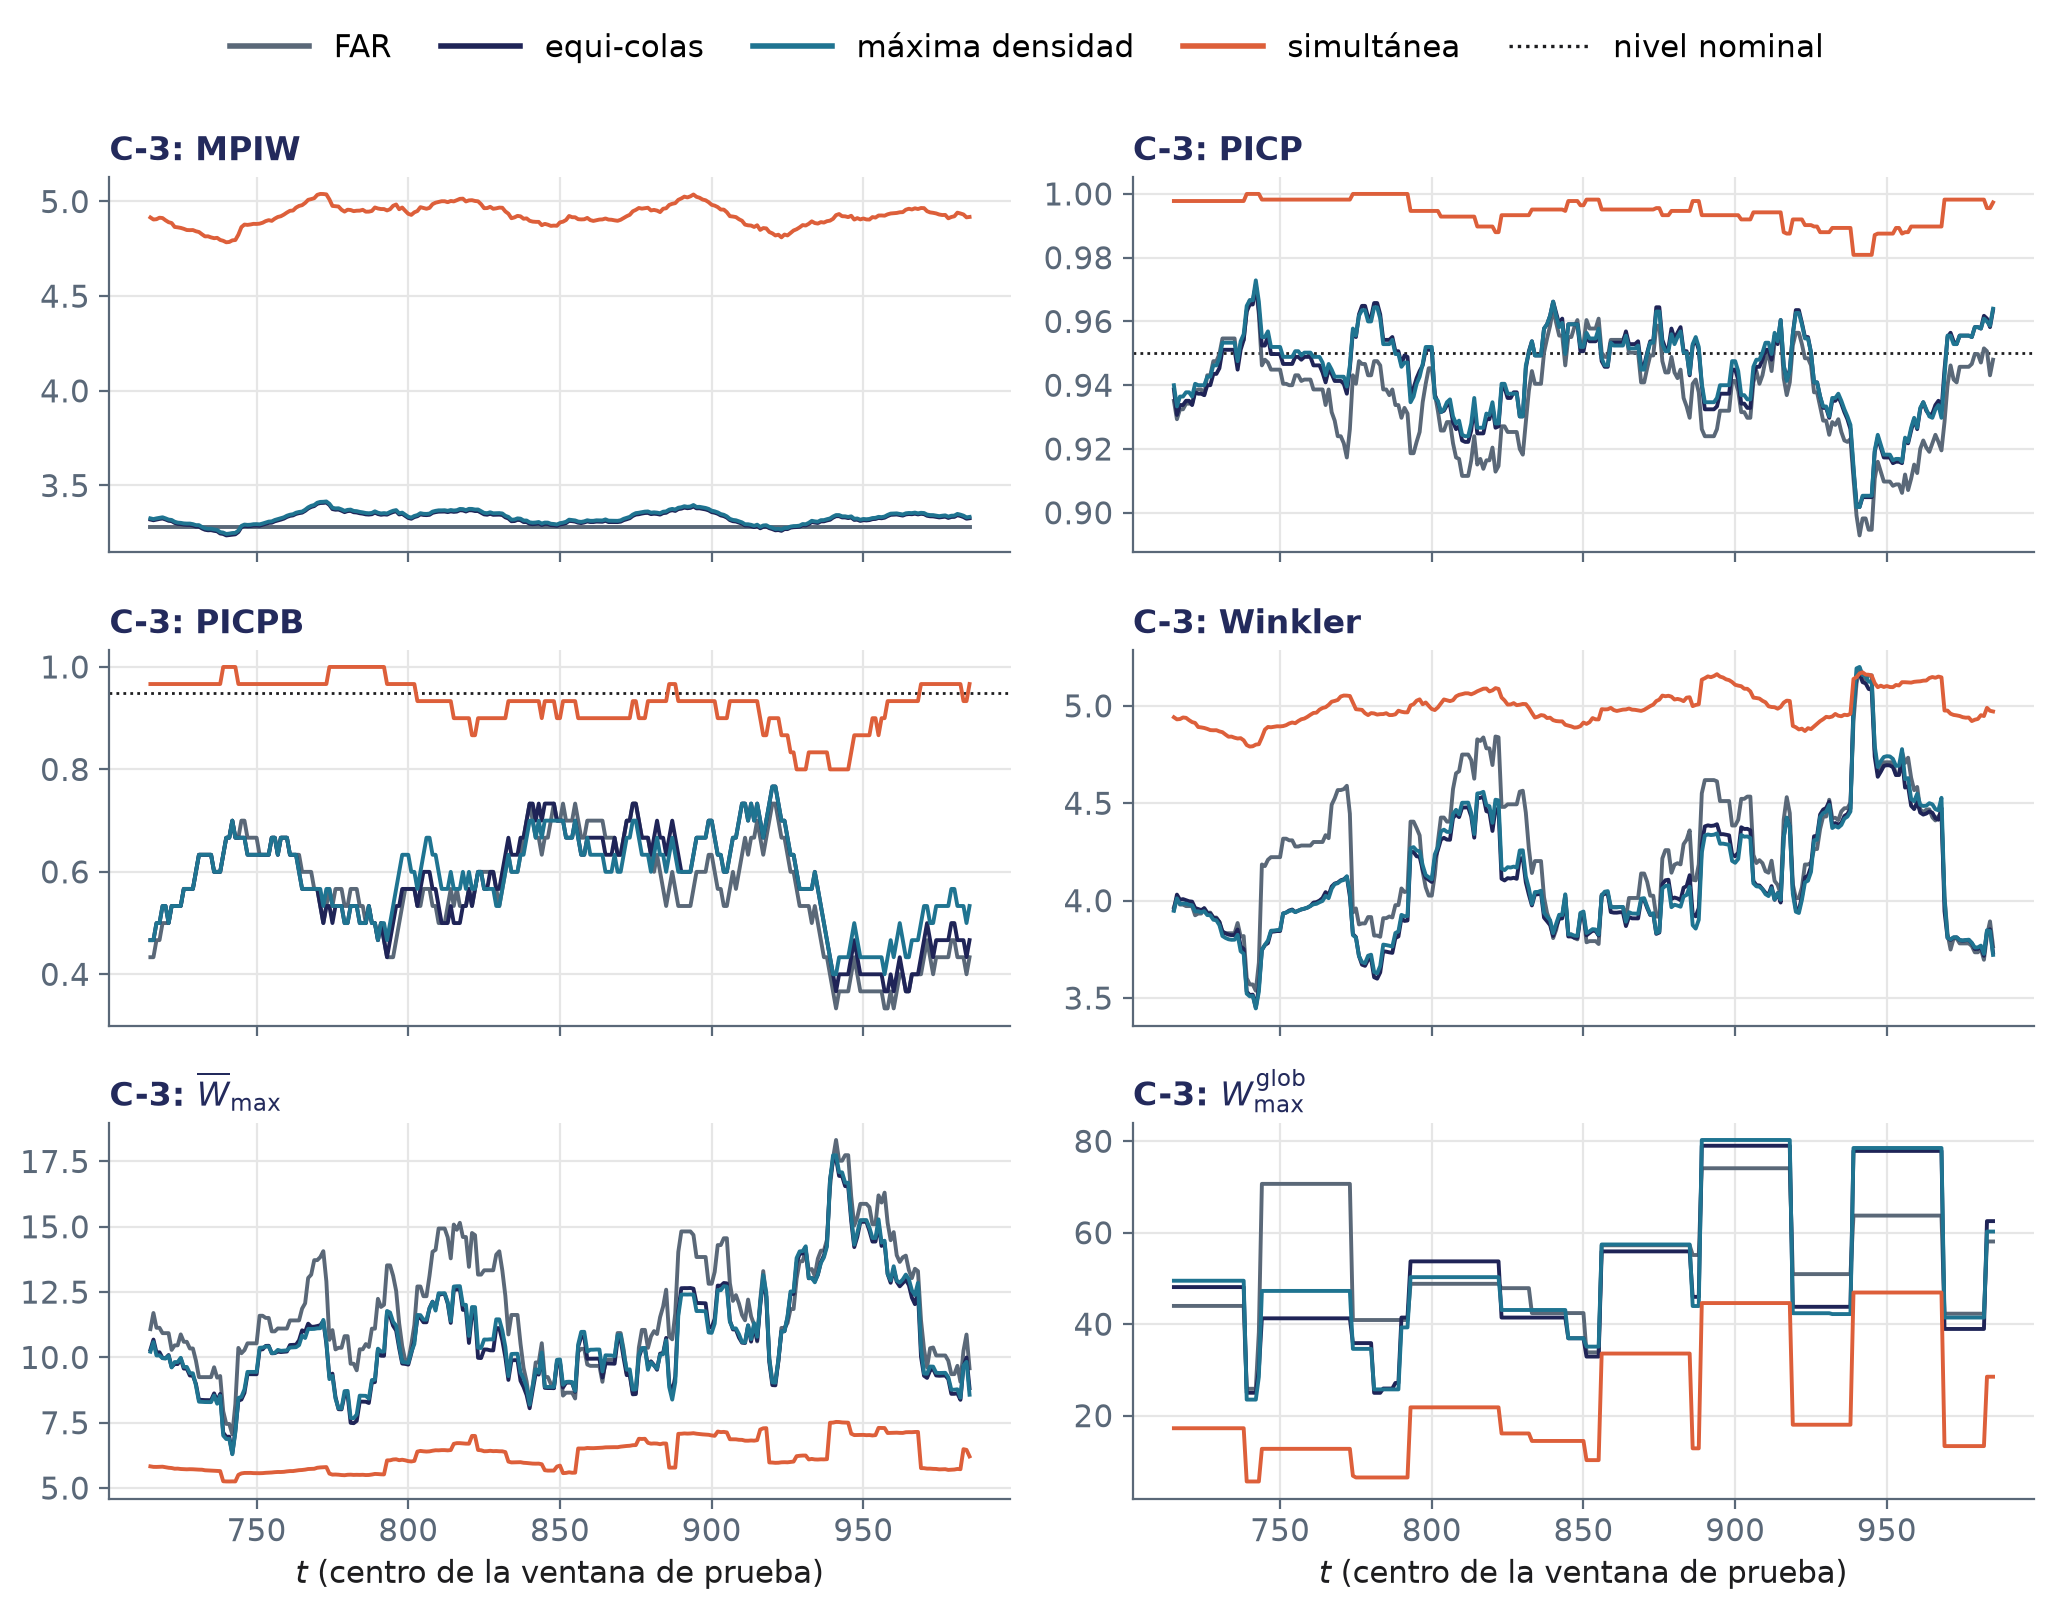
\includegraphics[width=\textwidth,height=0.75\textheight,keepaspectratio]{IMG/aneB_00/aneB_00_ventana_intervalos_w30_C3.png}
\caption{C-3 (multimodalidad). Métricas de intervalo sobre la ventana móvil ($M_{\mathrm{ref}}$).}
\label{fig:aneB_int_C3}
\end{figure}

\section{Calibración respecto de la representación truncada}
\label{aneB_00_04_calibracion_truncada}

Las métricas evaluadas contra la representación $X_t^{(M)}$ en lugar de la curva suavizada, en función de $M$.

\begin{figure}[H]
\centering
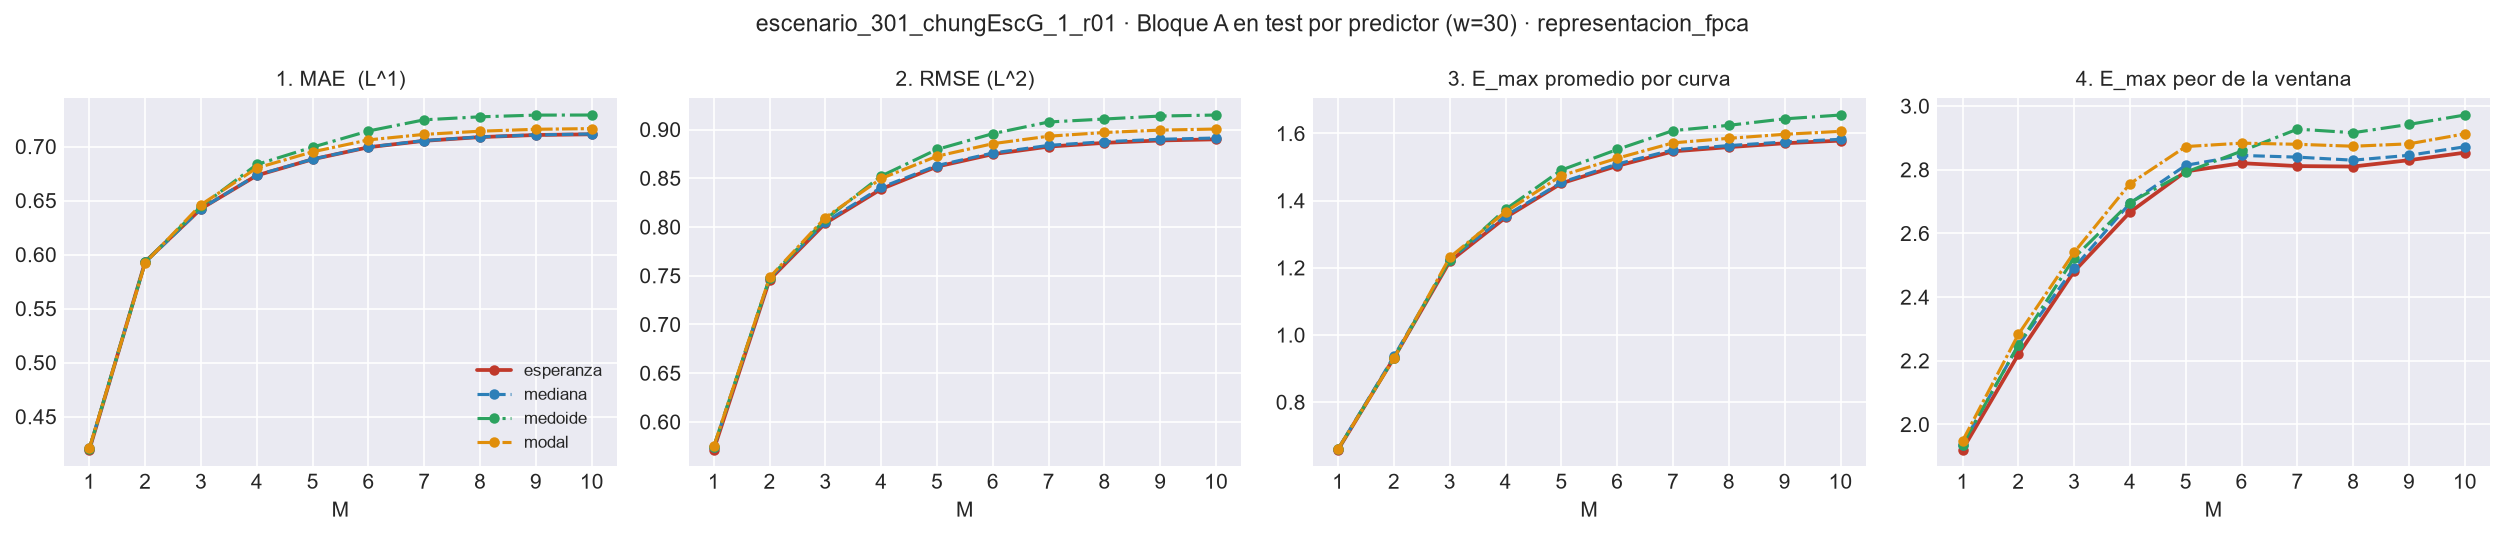
\includegraphics[width=\textwidth,height=0.4\textheight,keepaspectratio]{IMG/aneB_00/aneB_00_bloqueA_vs_M_repr_C1.png}
\caption{C-1 (GARCH). Métricas de error contra la representación truncada, por $M$.}
\label{fig:aneB_reprA_C1}
\end{figure}

\begin{figure}[H]
\centering
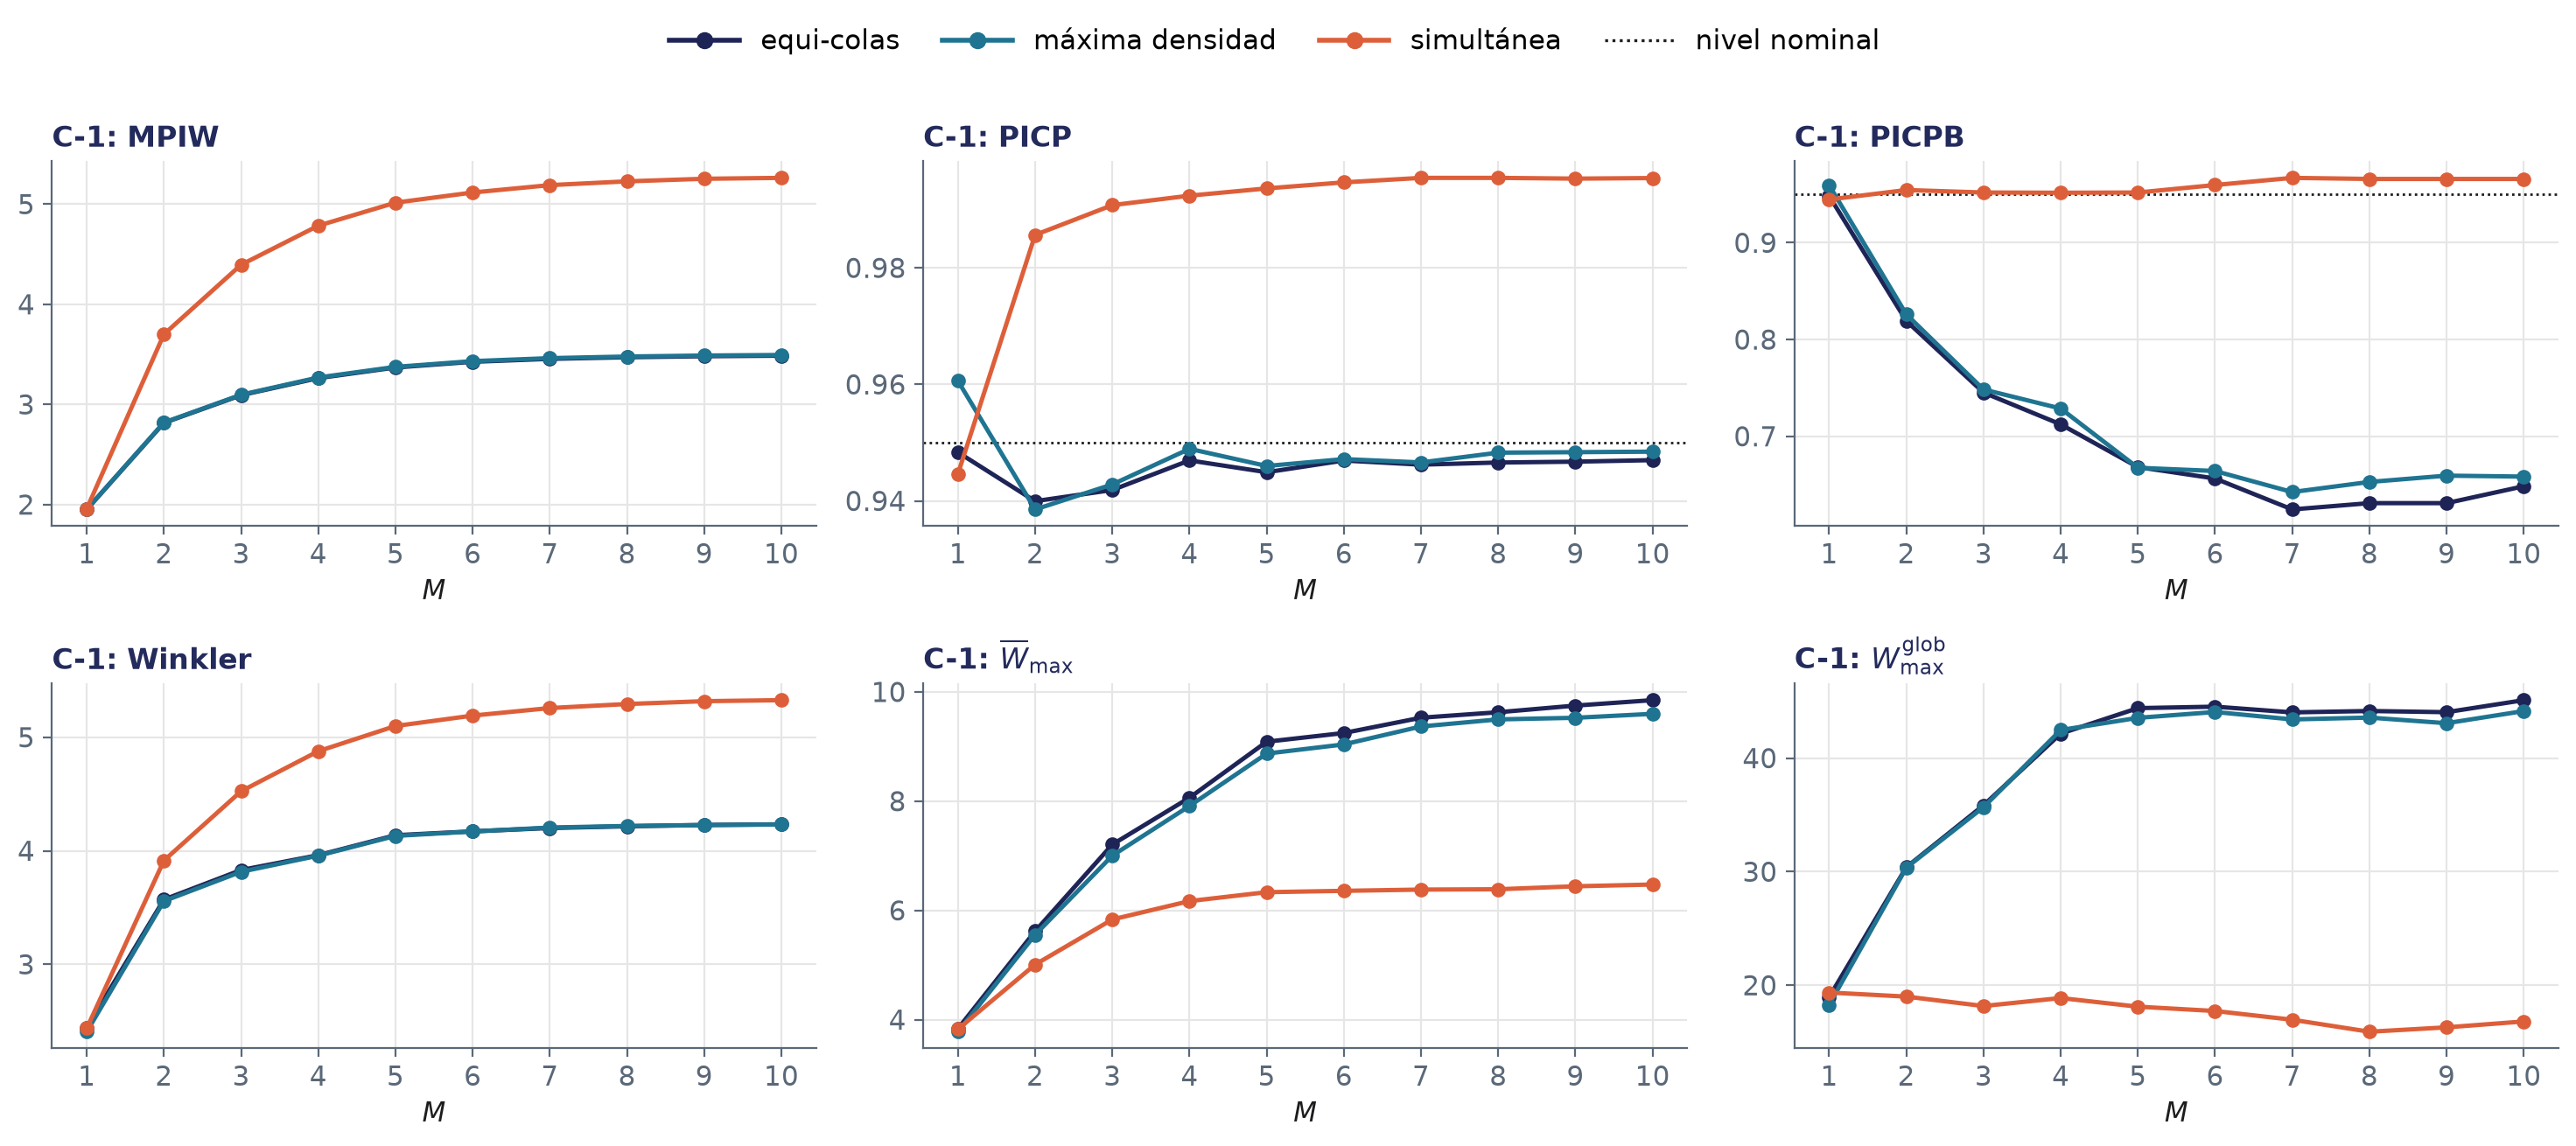
\includegraphics[width=\textwidth,height=0.4\textheight,keepaspectratio]{IMG/aneB_00/aneB_00_bloqueB_vs_M_repr_C1.png}
\caption{C-1 (GARCH). Métricas de intervalo contra la representación truncada, por $M$.}
\label{fig:aneB_reprB_C1}
\end{figure}

\begin{figure}[H]
\centering
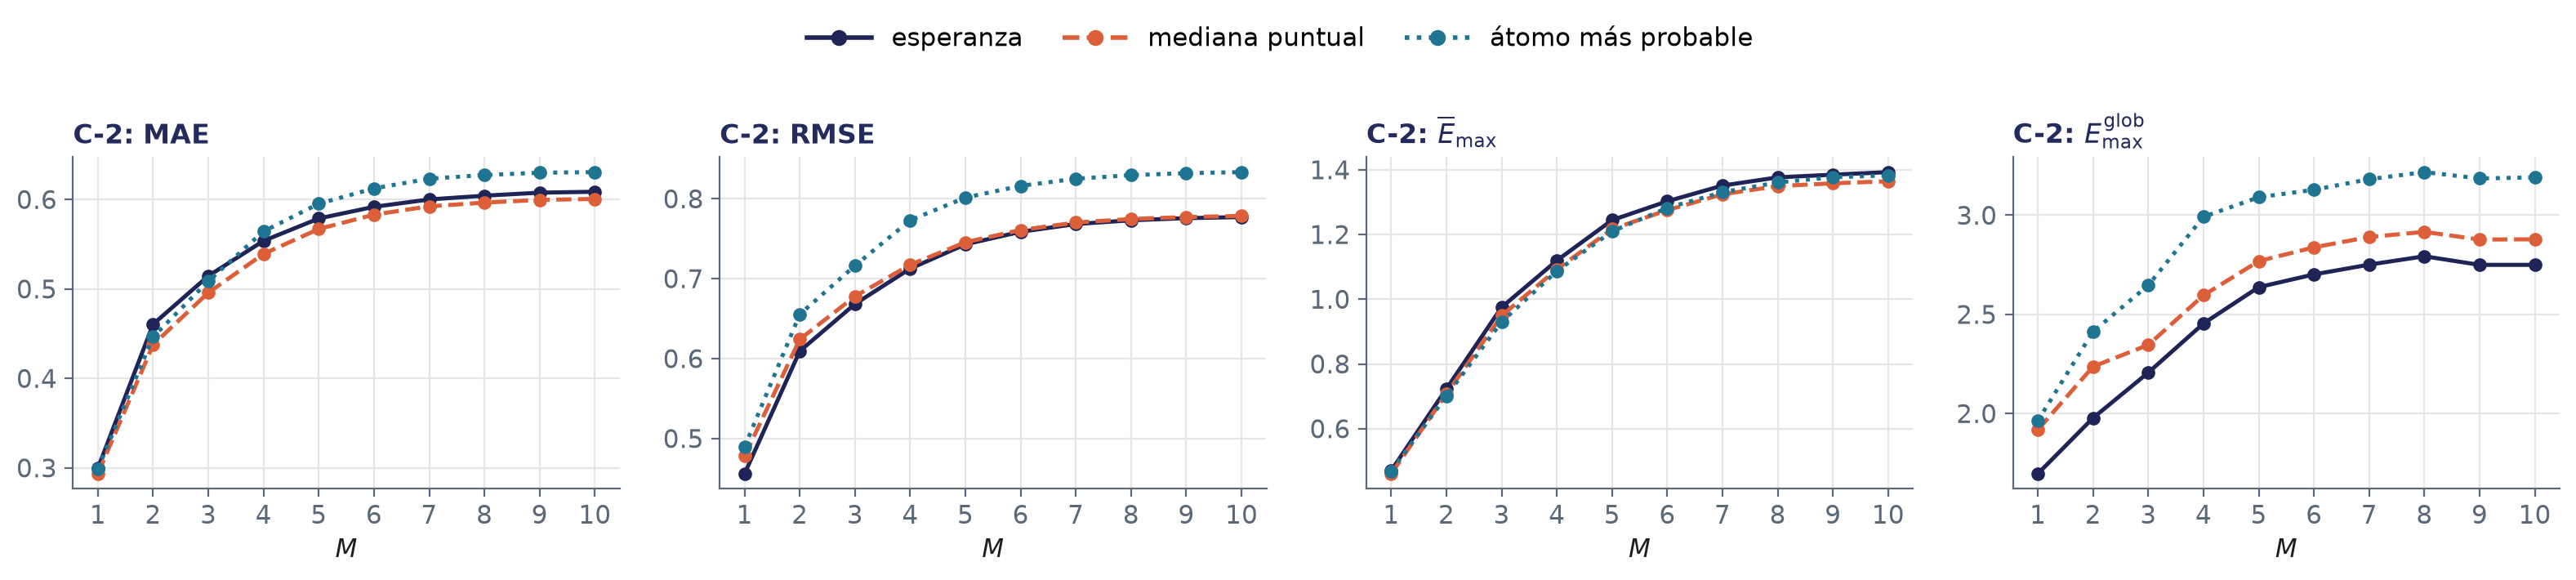
\includegraphics[width=\textwidth,height=0.4\textheight,keepaspectratio]{IMG/aneB_00/aneB_00_bloqueA_vs_M_repr_C2.png}
\caption{C-2 (TAR). Métricas de error contra la representación truncada, por $M$.}
\label{fig:aneB_reprA_C2}
\end{figure}

\begin{figure}[H]
\centering
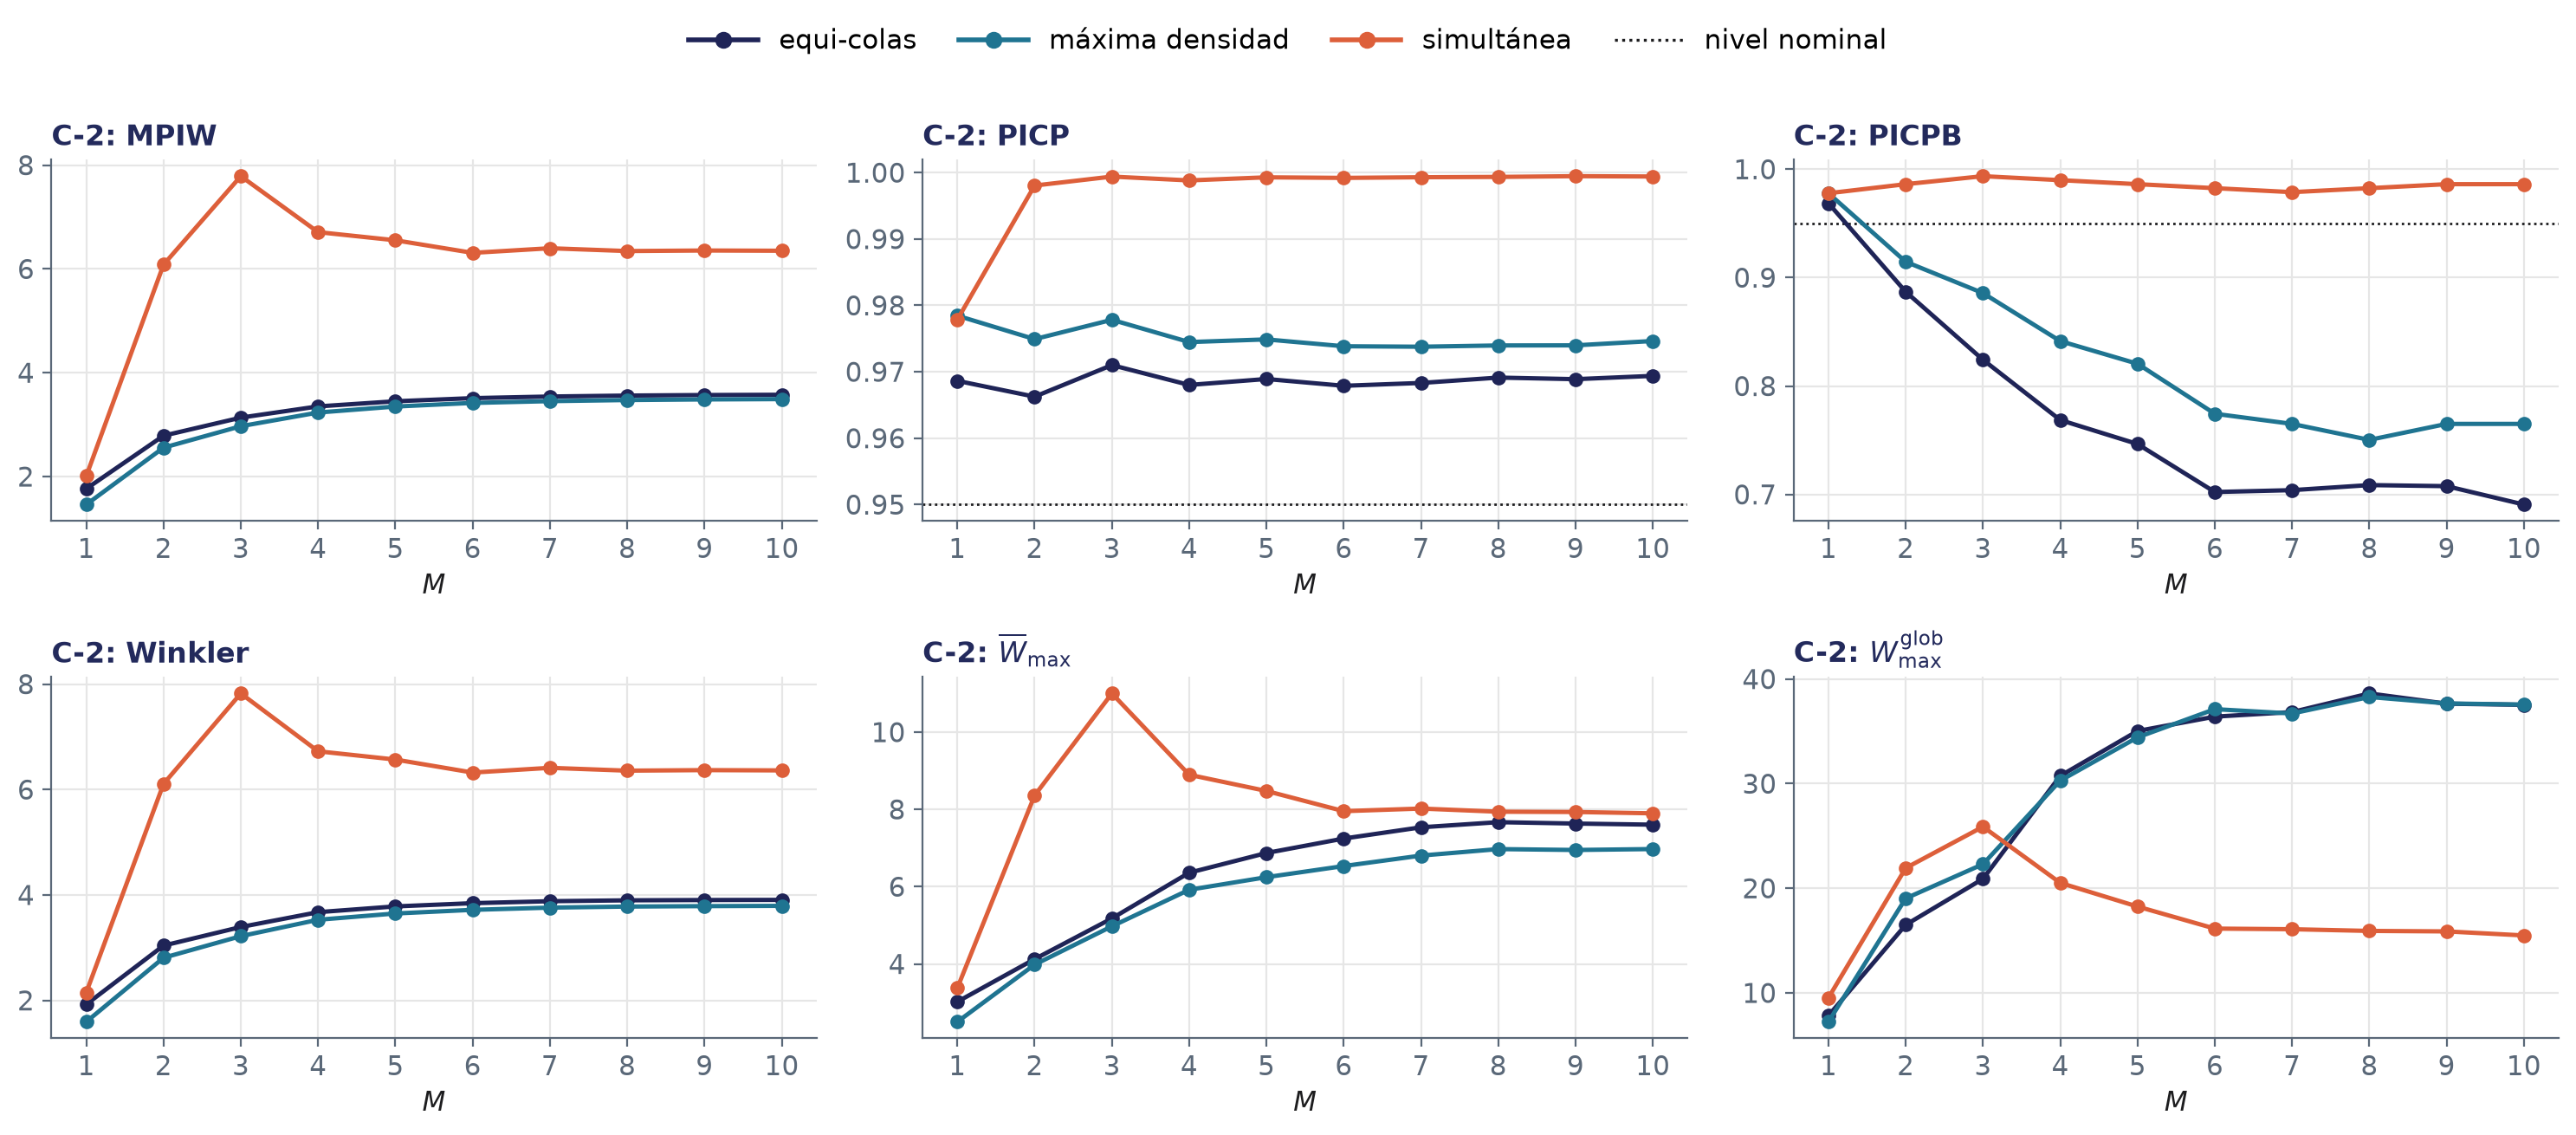
\includegraphics[width=\textwidth,height=0.4\textheight,keepaspectratio]{IMG/aneB_00/aneB_00_bloqueB_vs_M_repr_C2.png}
\caption{C-2 (TAR). Métricas de intervalo contra la representación truncada, por $M$.}
\label{fig:aneB_reprB_C2}
\end{figure}

\begin{figure}[H]
\centering
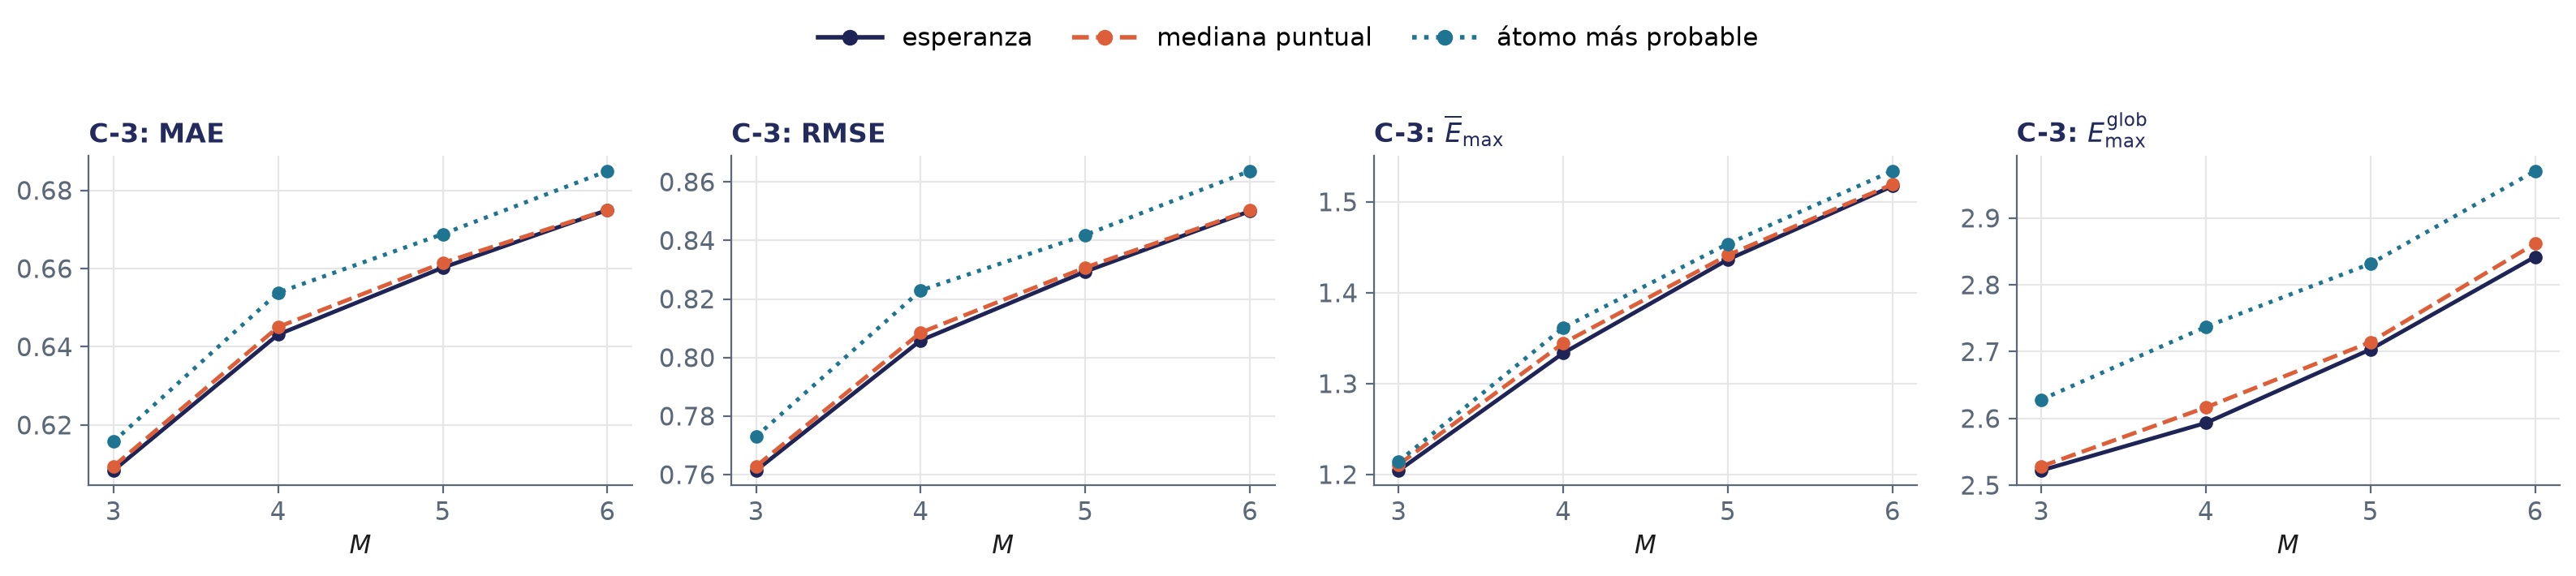
\includegraphics[width=\textwidth,height=0.4\textheight,keepaspectratio]{IMG/aneB_00/aneB_00_bloqueA_vs_M_repr_C3.png}
\caption{C-3 (multimodalidad). Métricas de error contra la representación truncada, por $M$.}
\label{fig:aneB_reprA_C3}
\end{figure}

\begin{figure}[H]
\centering
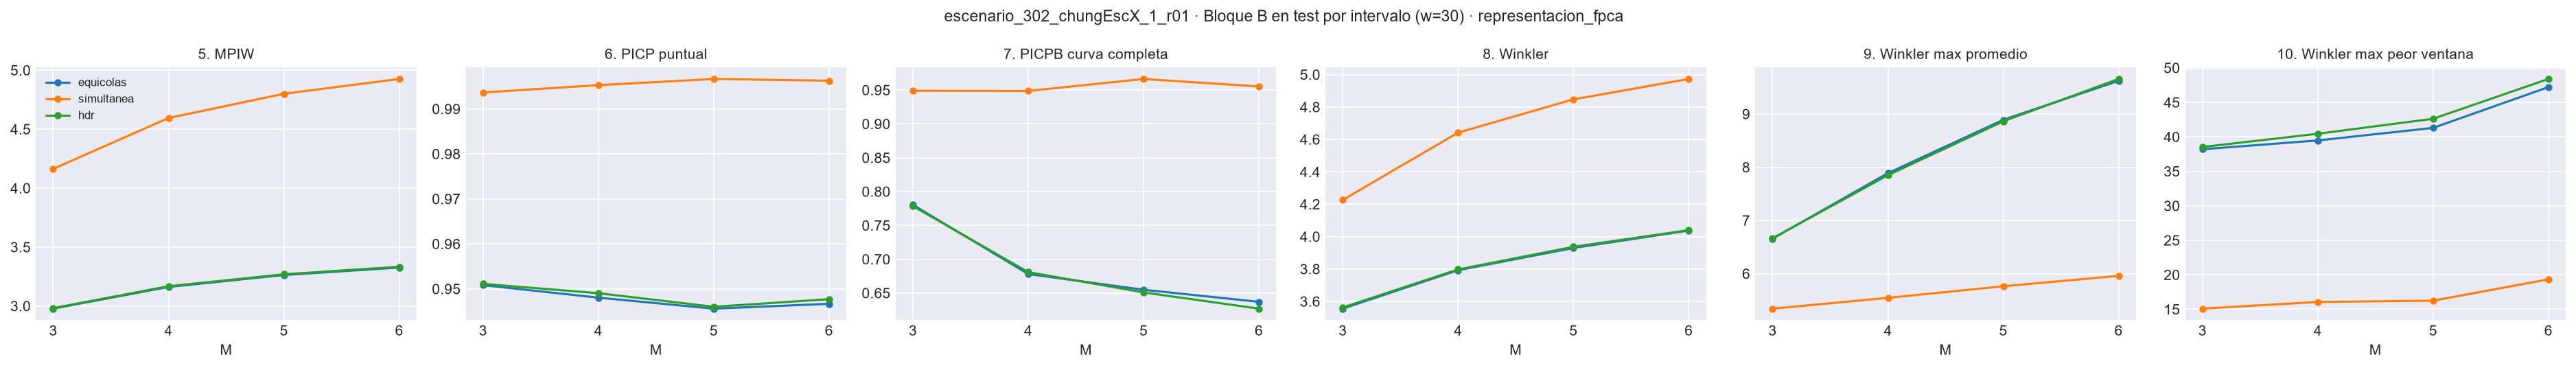
\includegraphics[width=\textwidth,height=0.4\textheight,keepaspectratio]{IMG/aneB_00/aneB_00_bloqueB_vs_M_repr_C3.png}
\caption{C-3 (multimodalidad). Métricas de intervalo contra la representación truncada, por $M$.}
\label{fig:aneB_reprB_C3}
\end{figure}

\section{Intervalos por componente}
\label{aneB_00_05_intervalos_componente}

Banda de credibilidad al 95\% de cada score y dispersión estimada frente a la observada.

\begin{figure}[H]
\centering
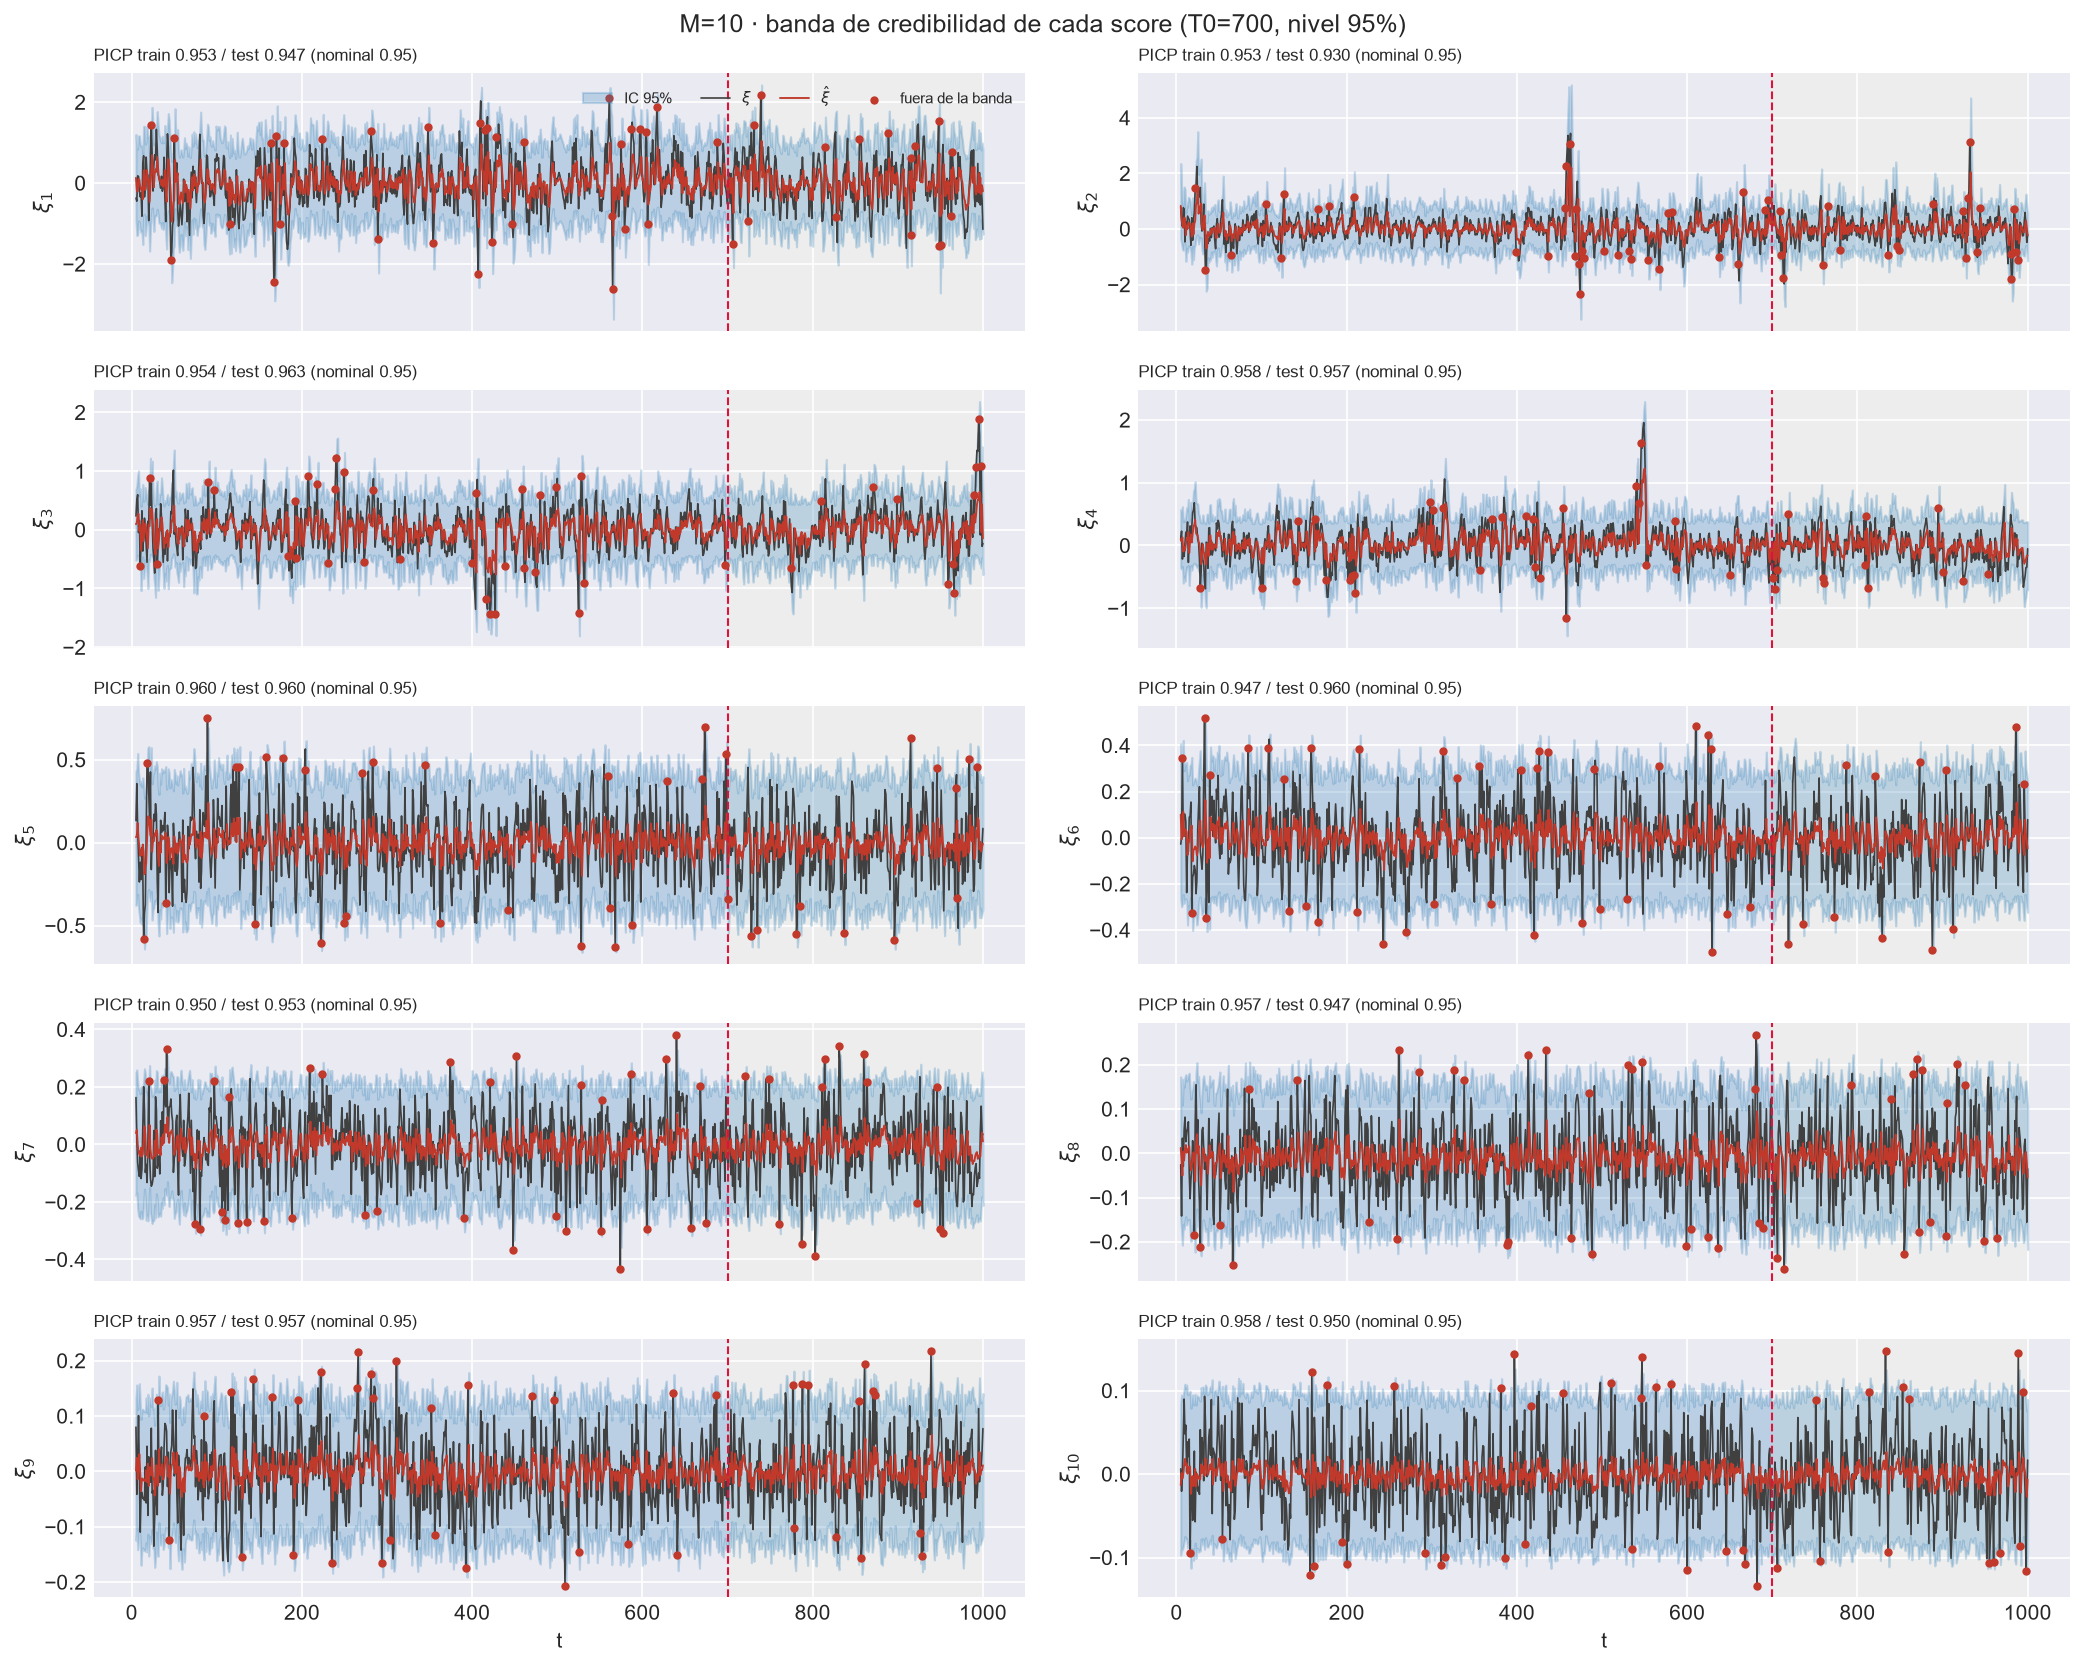
\includegraphics[width=\textwidth,height=0.7\textheight,keepaspectratio]{IMG/aneB_00/aneB_00_scores_banda_C1.png}
\caption{C-1 (GARCH). Banda de credibilidad de cada score ($M_{\mathrm{ref}}$).}
\label{fig:aneB_banda_C1}
\end{figure}

\begin{figure}[H]
\centering
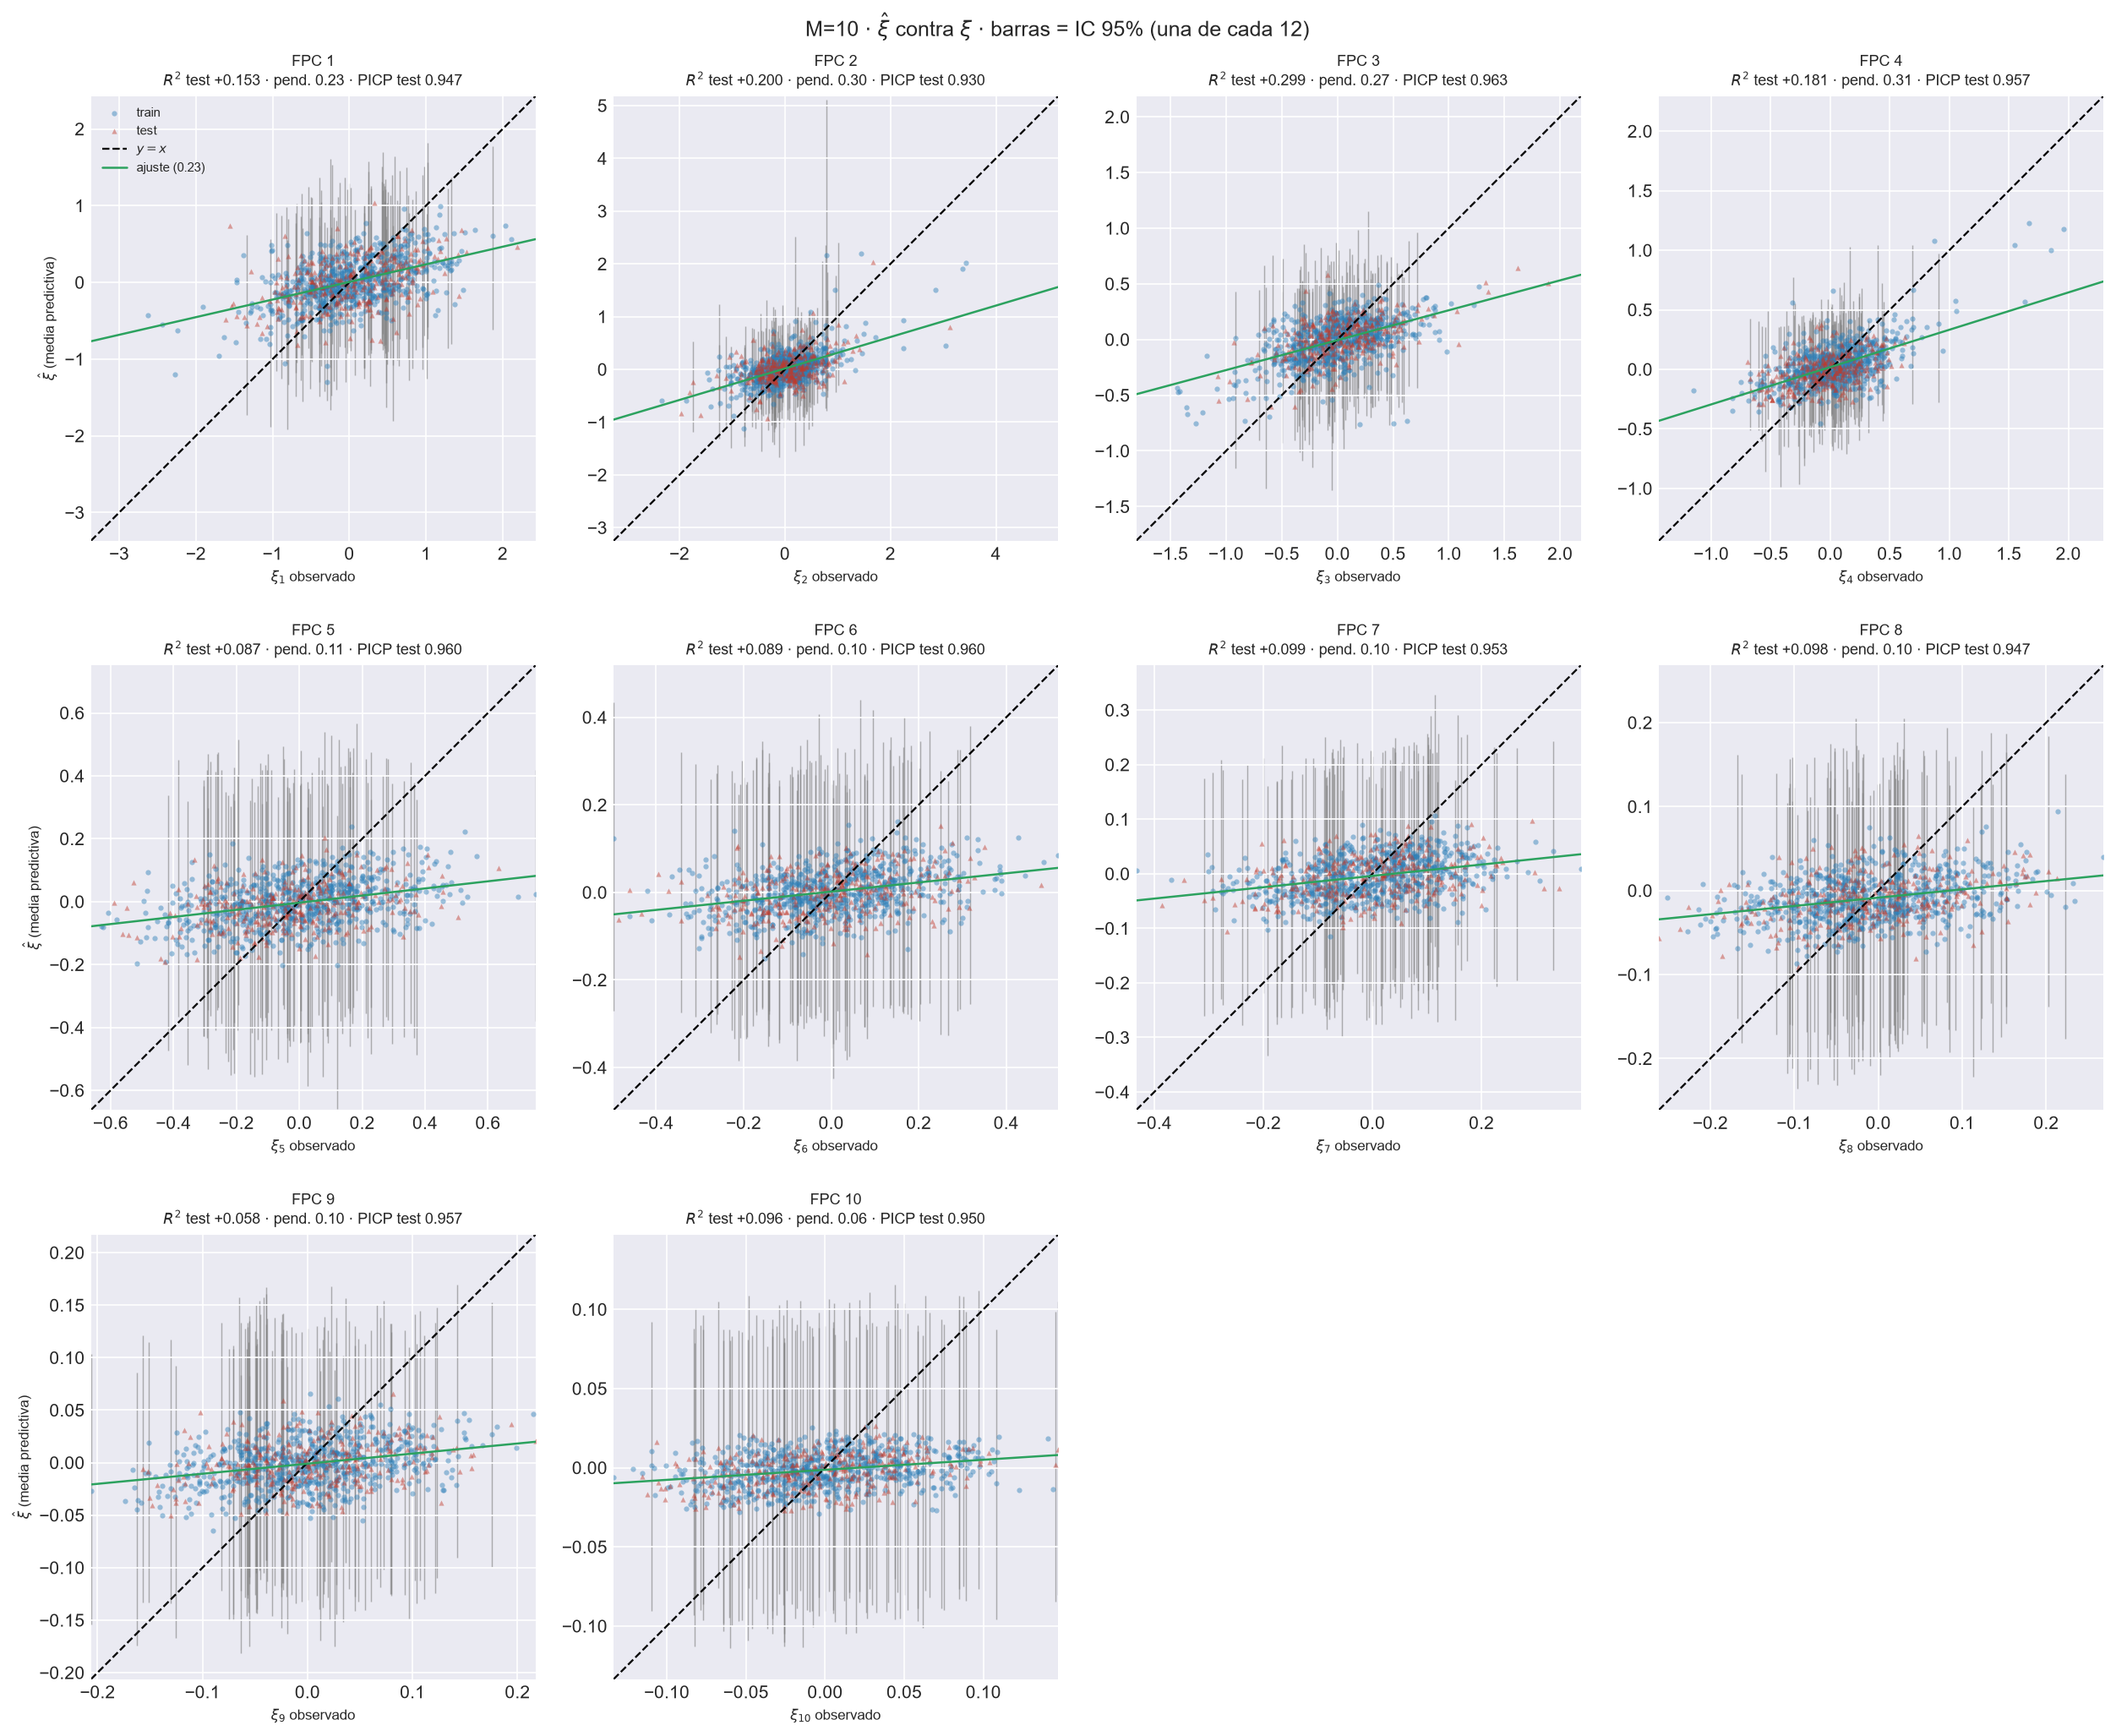
\includegraphics[width=\textwidth,height=0.7\textheight,keepaspectratio]{IMG/aneB_00/aneB_00_scores_dispersion_C1.png}
\caption{C-1 (GARCH). Dispersión estimada de cada score frente a la observada ($M_{\mathrm{ref}}$).}
\label{fig:aneB_disp_C1}
\end{figure}

\begin{figure}[H]
\centering
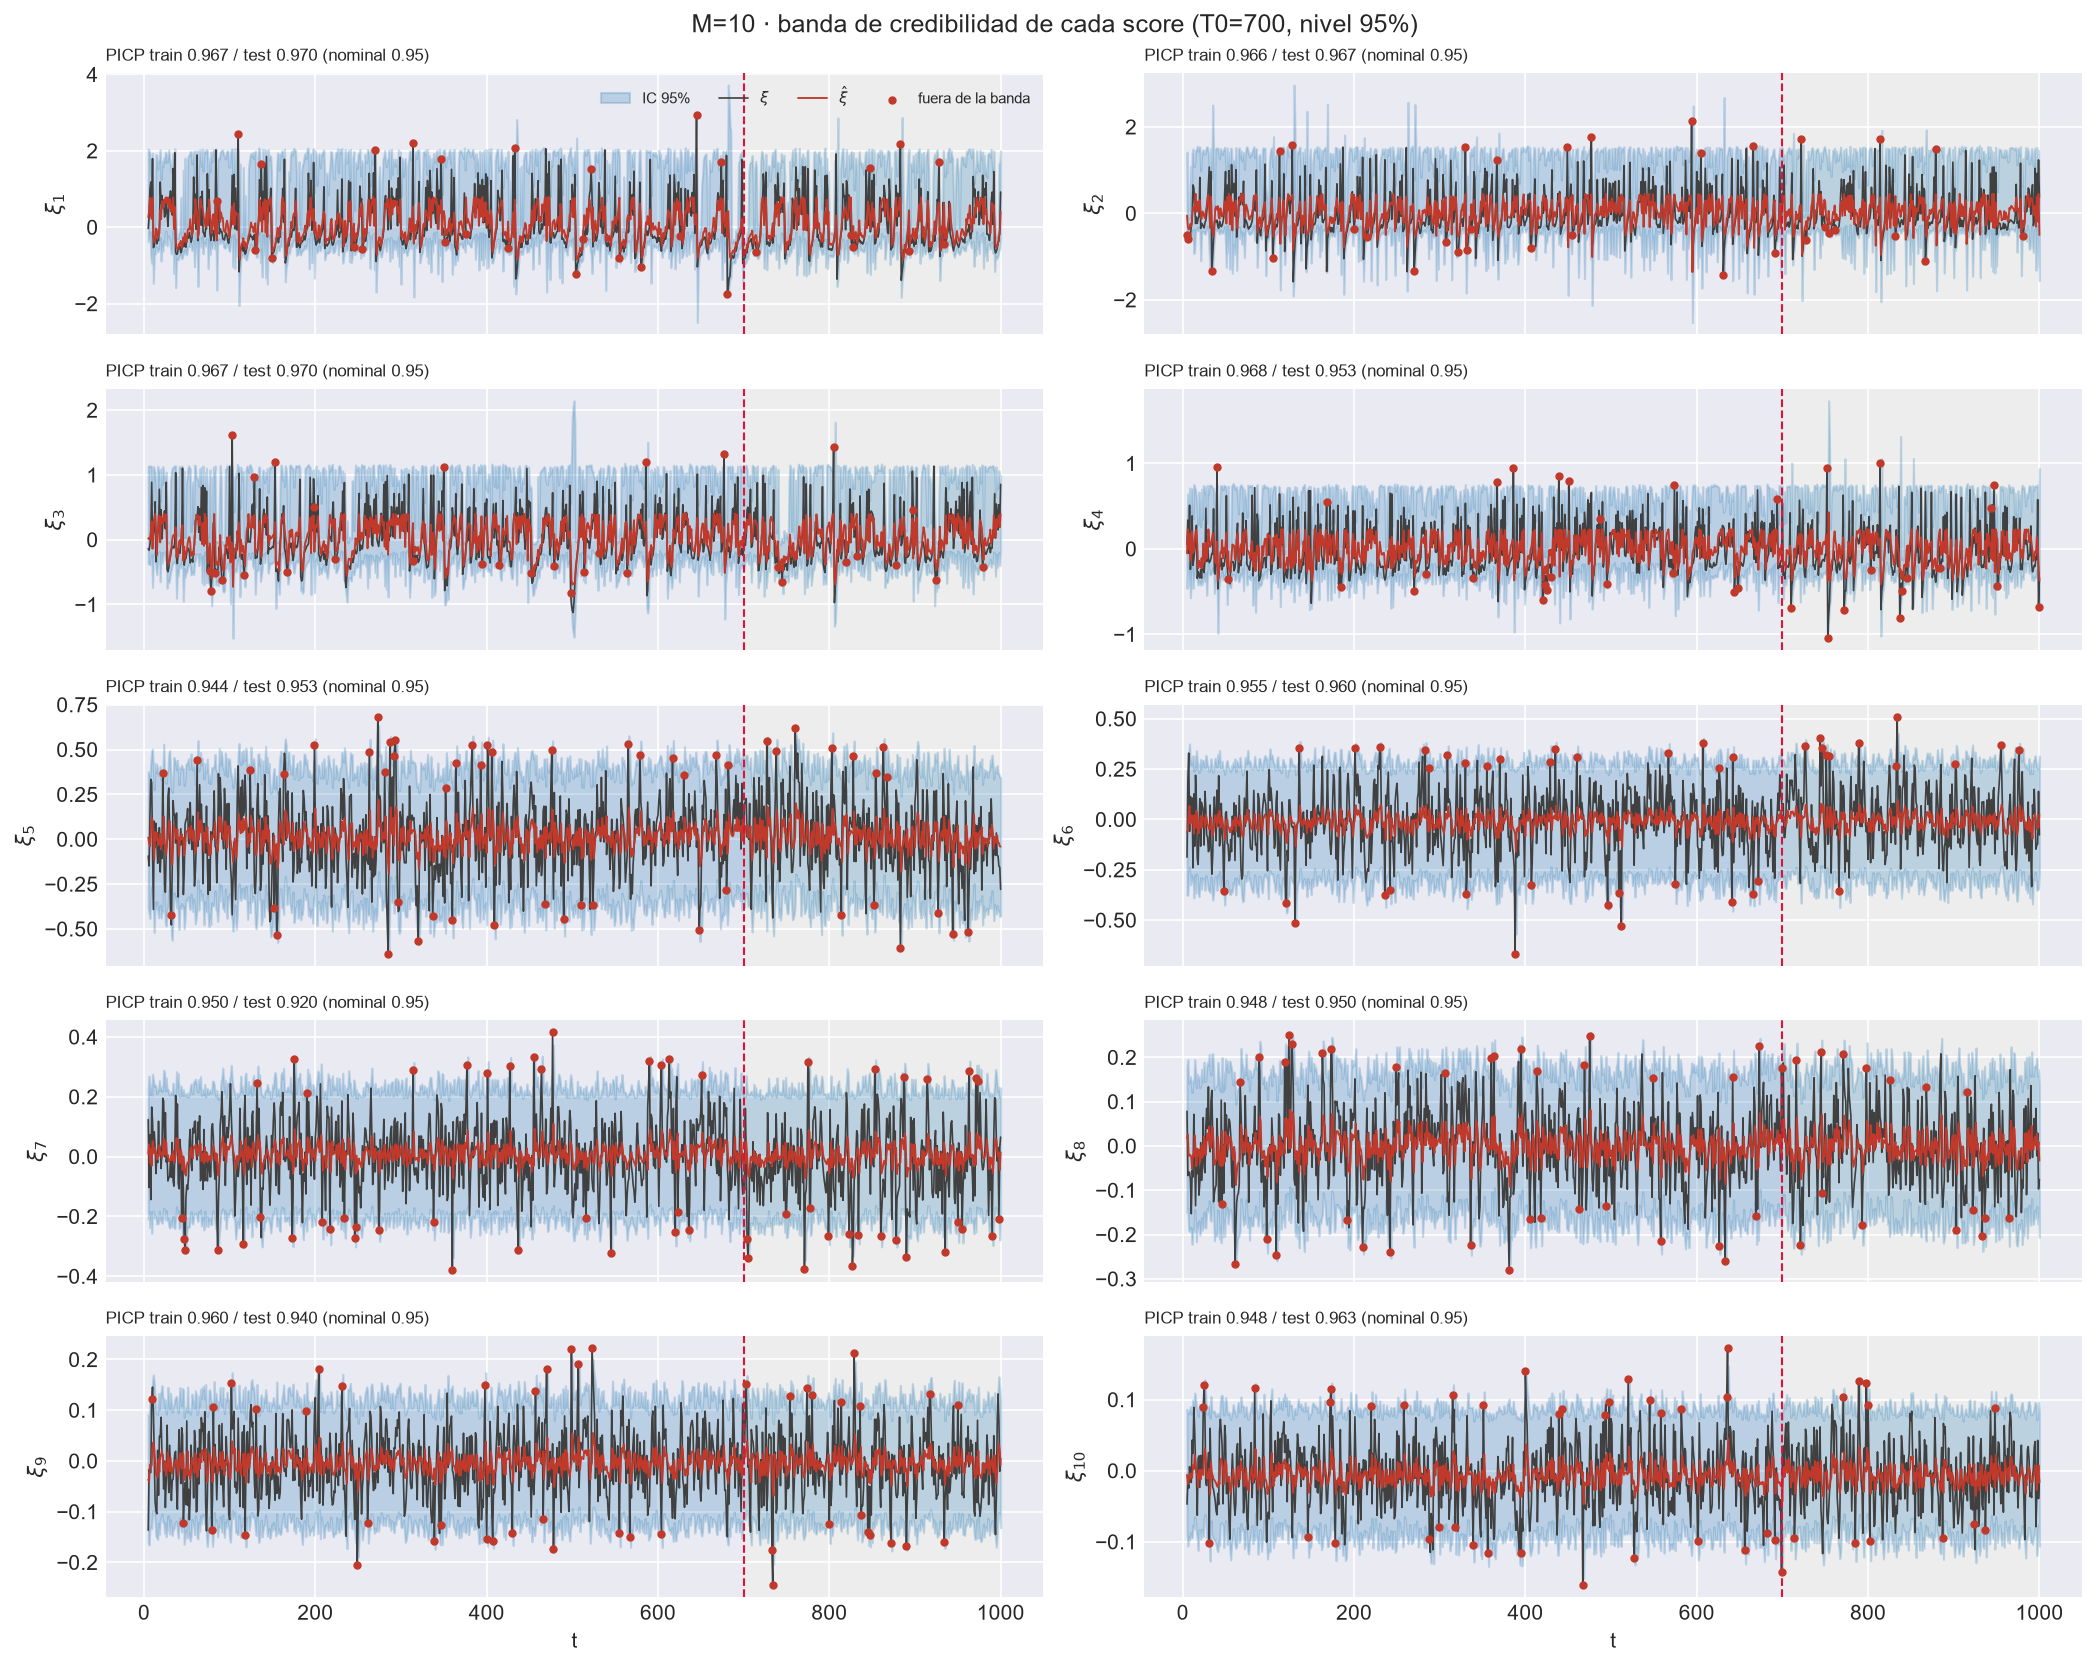
\includegraphics[width=\textwidth,height=0.7\textheight,keepaspectratio]{IMG/aneB_00/aneB_00_scores_banda_C2.png}
\caption{C-2 (TAR). Banda de credibilidad de cada score ($M_{\mathrm{ref}}$).}
\label{fig:aneB_banda_C2}
\end{figure}

\begin{figure}[H]
\centering
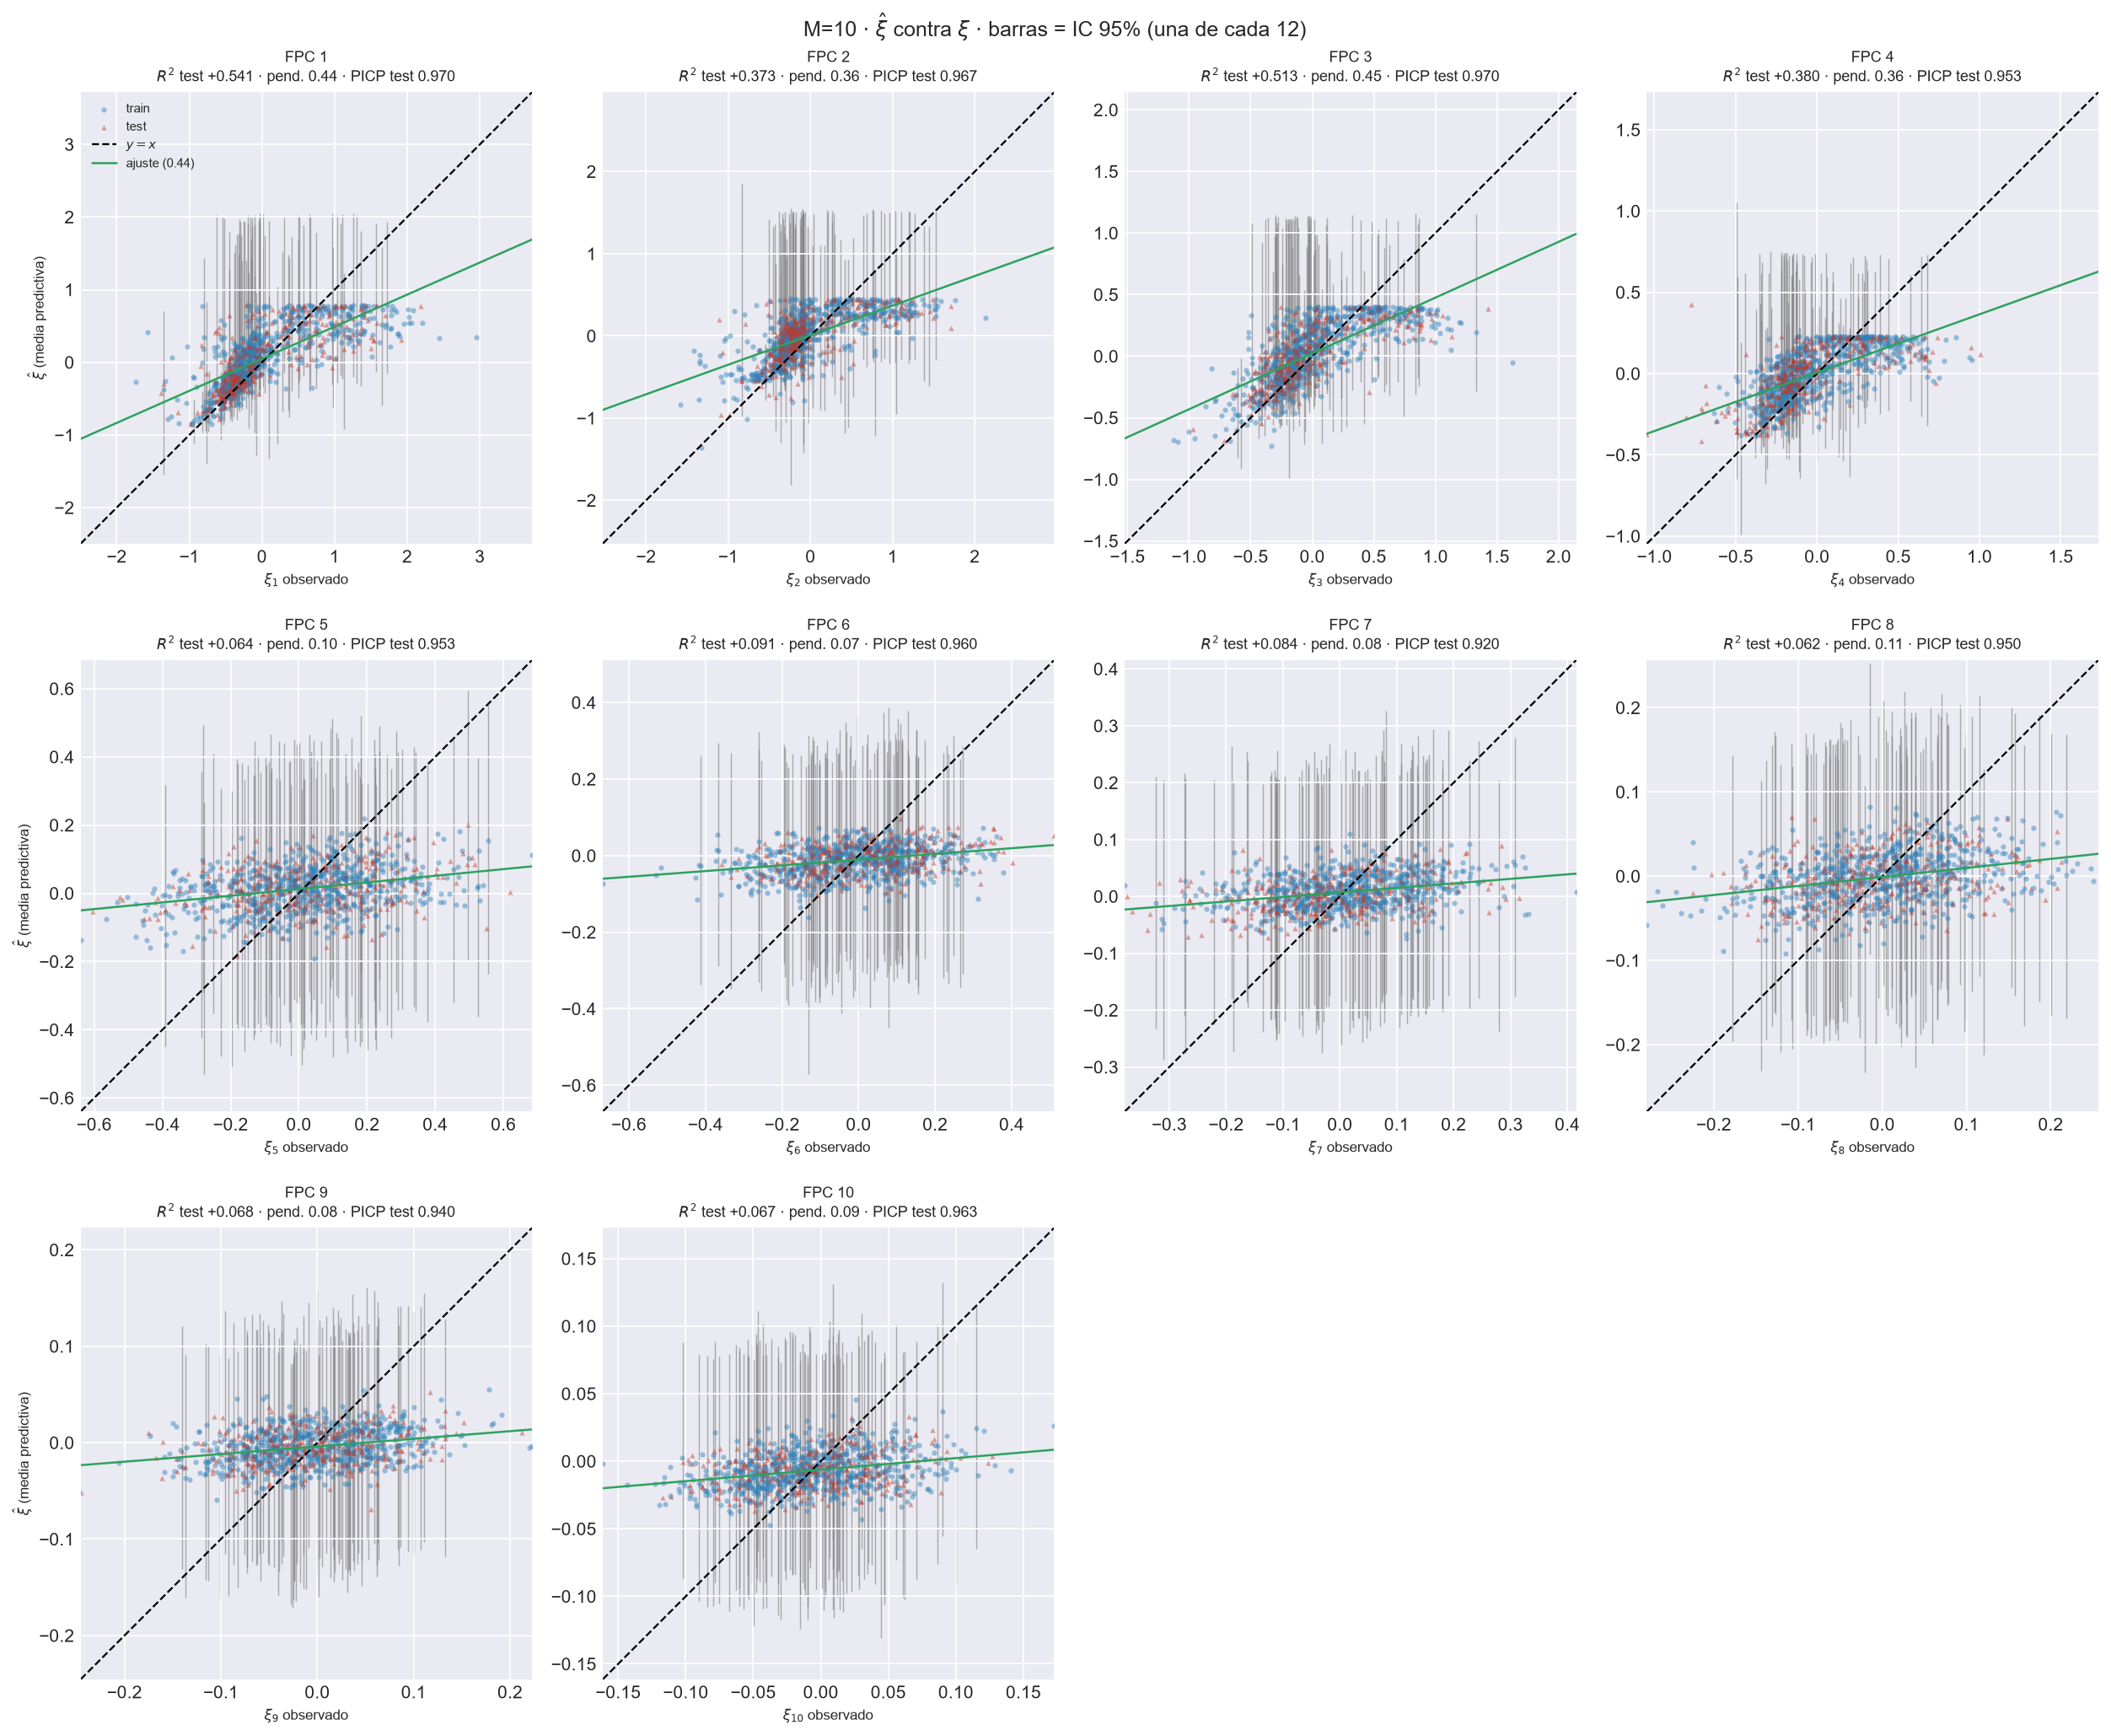
\includegraphics[width=\textwidth,height=0.7\textheight,keepaspectratio]{IMG/aneB_00/aneB_00_scores_dispersion_C2.png}
\caption{C-2 (TAR). Dispersión estimada de cada score frente a la observada ($M_{\mathrm{ref}}$).}
\label{fig:aneB_disp_C2}
\end{figure}

\begin{figure}[H]
\centering
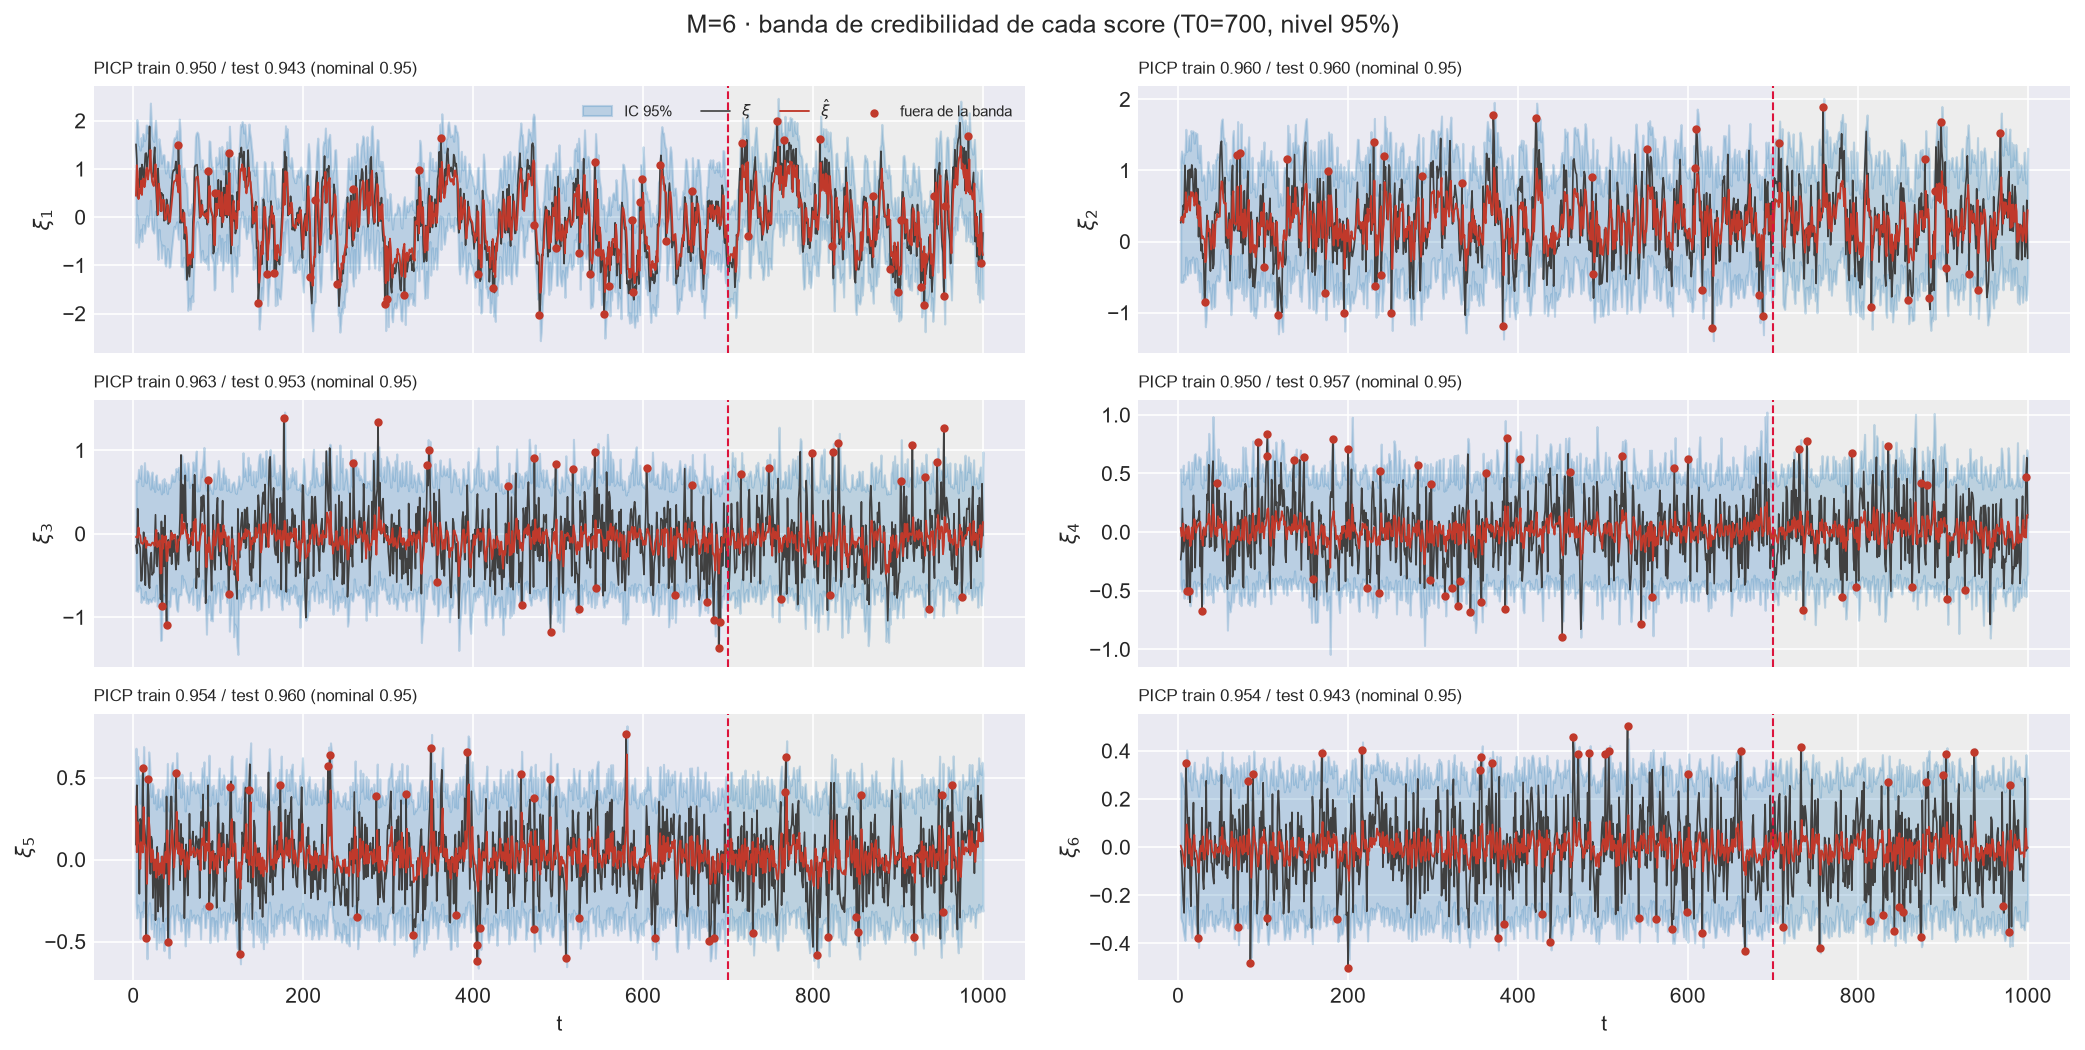
\includegraphics[width=\textwidth,height=0.7\textheight,keepaspectratio]{IMG/aneB_00/aneB_00_scores_banda_C3.png}
\caption{C-3 (multimodalidad). Banda de credibilidad de cada score ($M_{\mathrm{ref}}$).}
\label{fig:aneB_banda_C3}
\end{figure}

\begin{figure}[H]
\centering
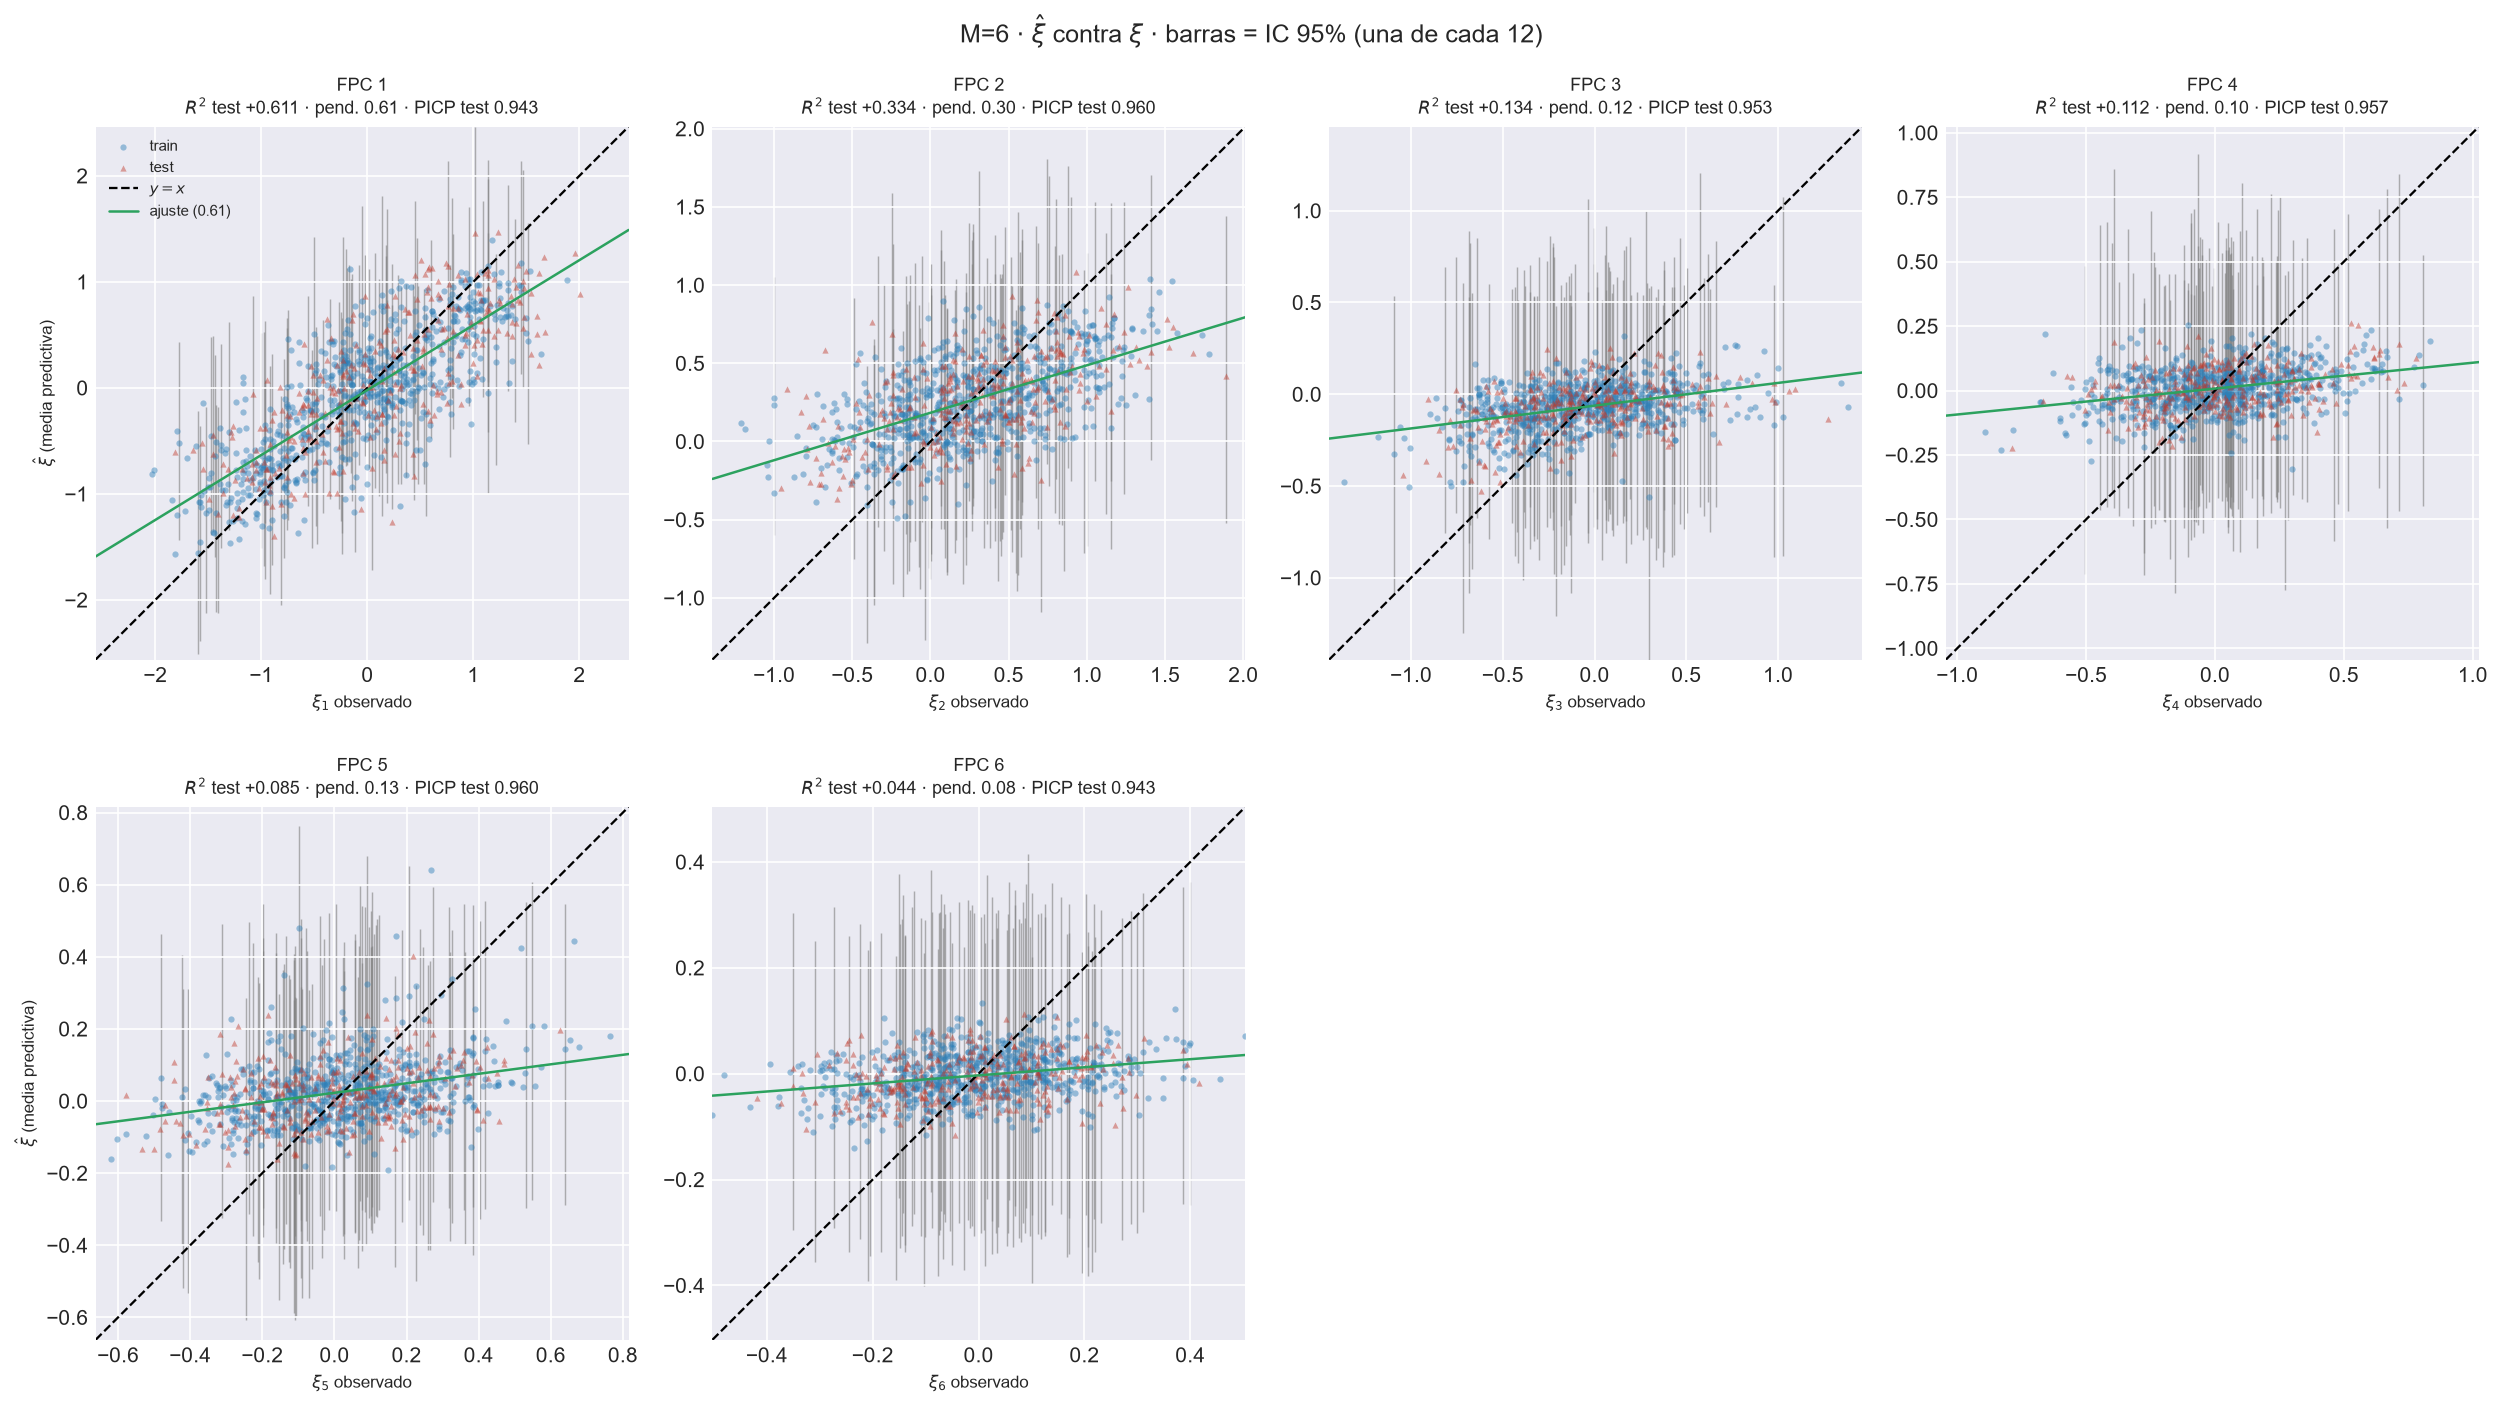
\includegraphics[width=\textwidth,height=0.7\textheight,keepaspectratio]{IMG/aneB_00/aneB_00_scores_dispersion_C3.png}
\caption{C-3 (multimodalidad). Dispersión estimada de cada score frente a la observada ($M_{\mathrm{ref}}$).}
\label{fig:aneB_disp_C3}
\end{figure}

\section{Predicciones curva a curva}
\label{aneB_00_06_predicciones_curvas}

Extractos de predicciones del bloque de prueba y orígenes de mejor y peor desempeño del PSBPM-FD frente al FAR.

\subsection{Escenario C-1 (GARCH)}
\label{aneB_00_06_02_curvas_garch}

\begin{figure}[H]
\centering
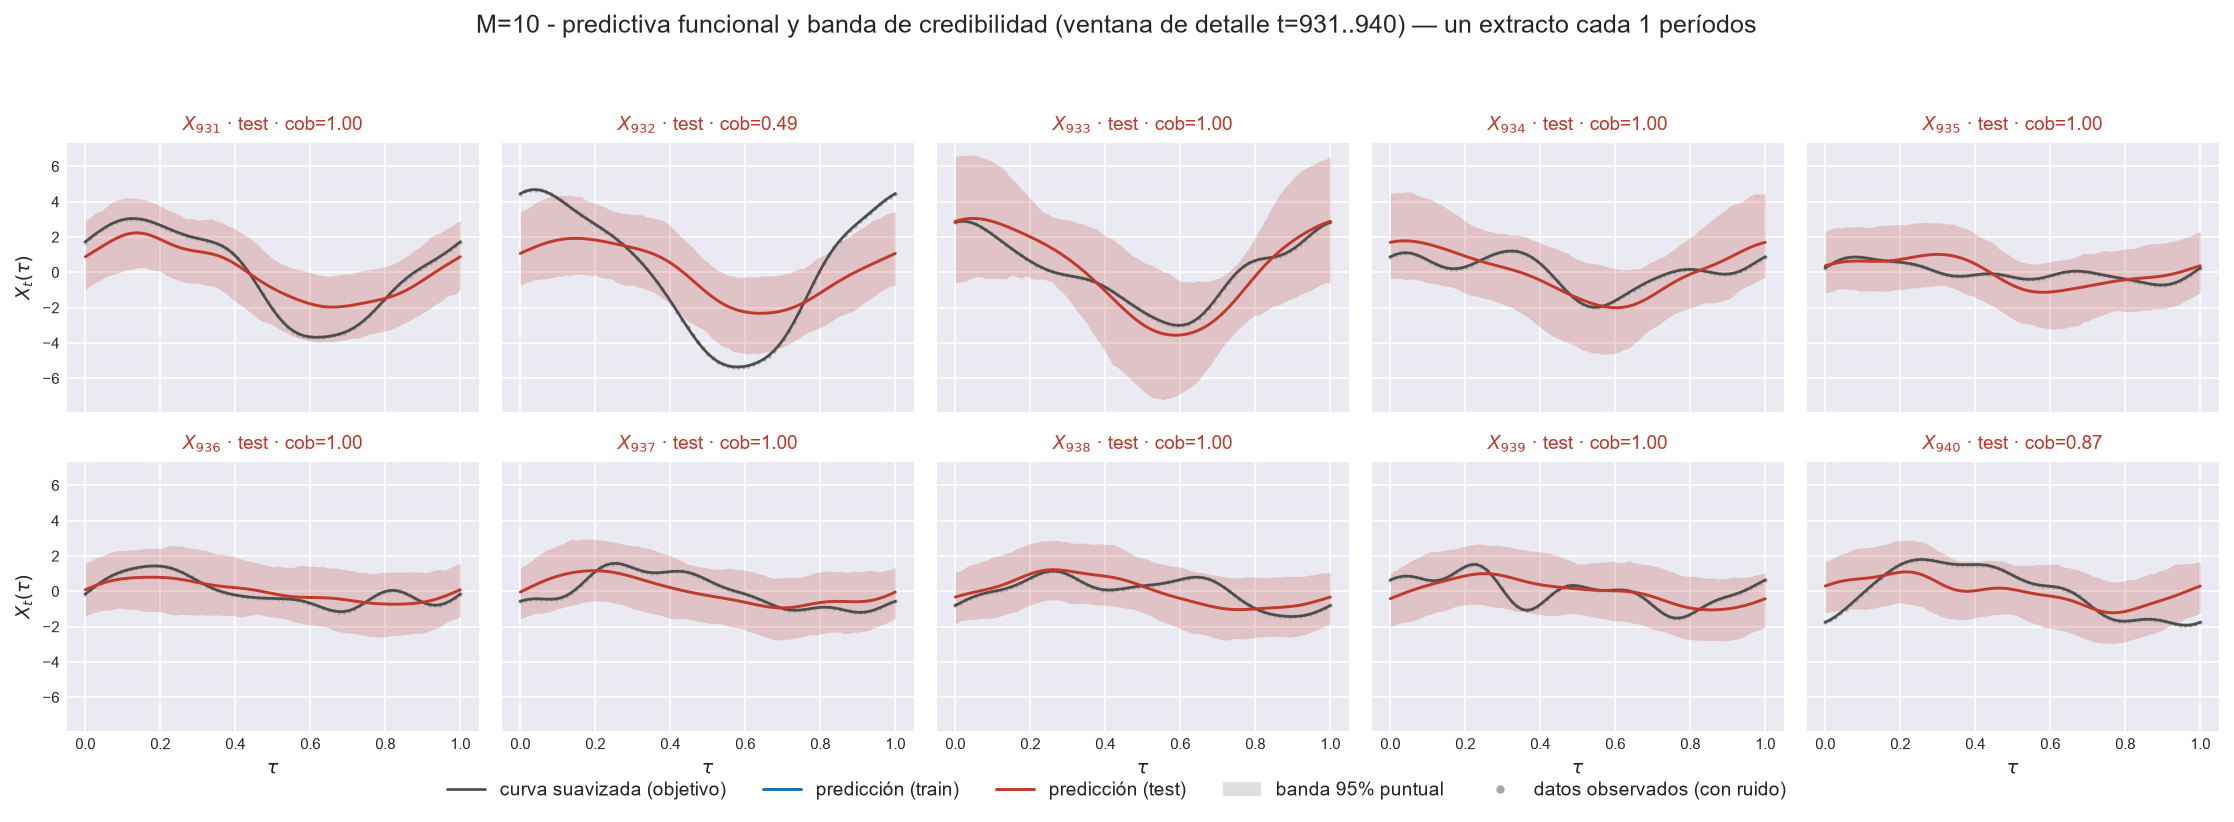
\includegraphics[width=\textwidth,height=0.45\textheight,keepaspectratio]{IMG/aneB_00/aneB_00_curvas_ext_C1.png}
\caption{C-1 (GARCH). Extractos de curvas del bloque de prueba con la predicción y su banda.}
\label{fig:aneB_curvas_ext_C1}
\end{figure}

\begin{figure}[H]
\centering
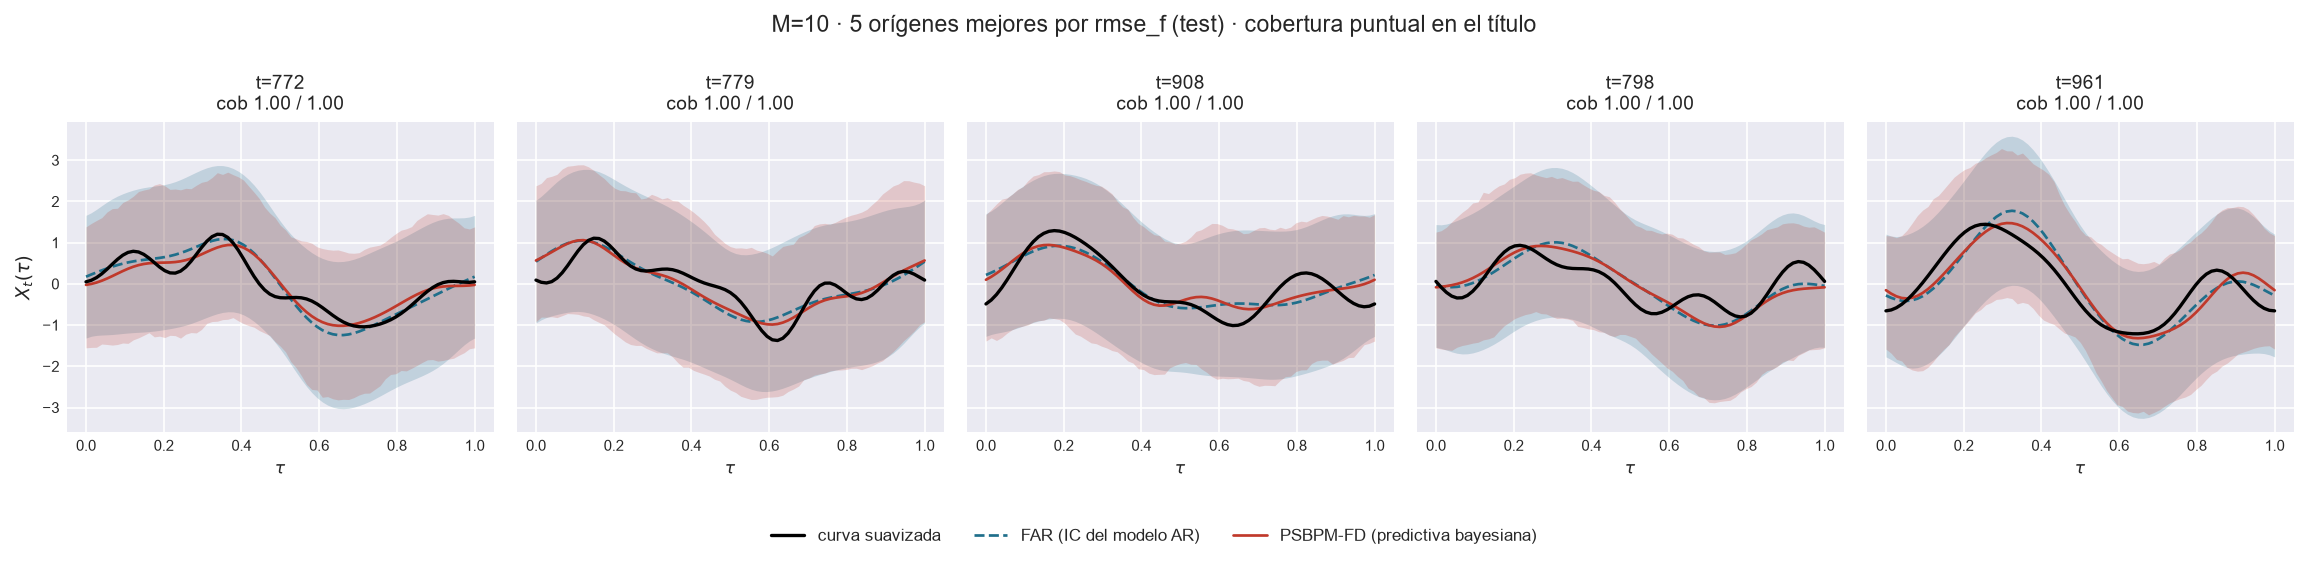
\includegraphics[width=\textwidth,height=0.45\textheight,keepaspectratio]{IMG/aneB_00/aneB_00_curvas_mej_C1.png}
\caption{C-1 (GARCH). Orígenes con mejor desempeño del PSBPM-FD frente al FAR.}
\label{fig:aneB_curvas_mej_C1}
\end{figure}

\begin{figure}[H]
\centering
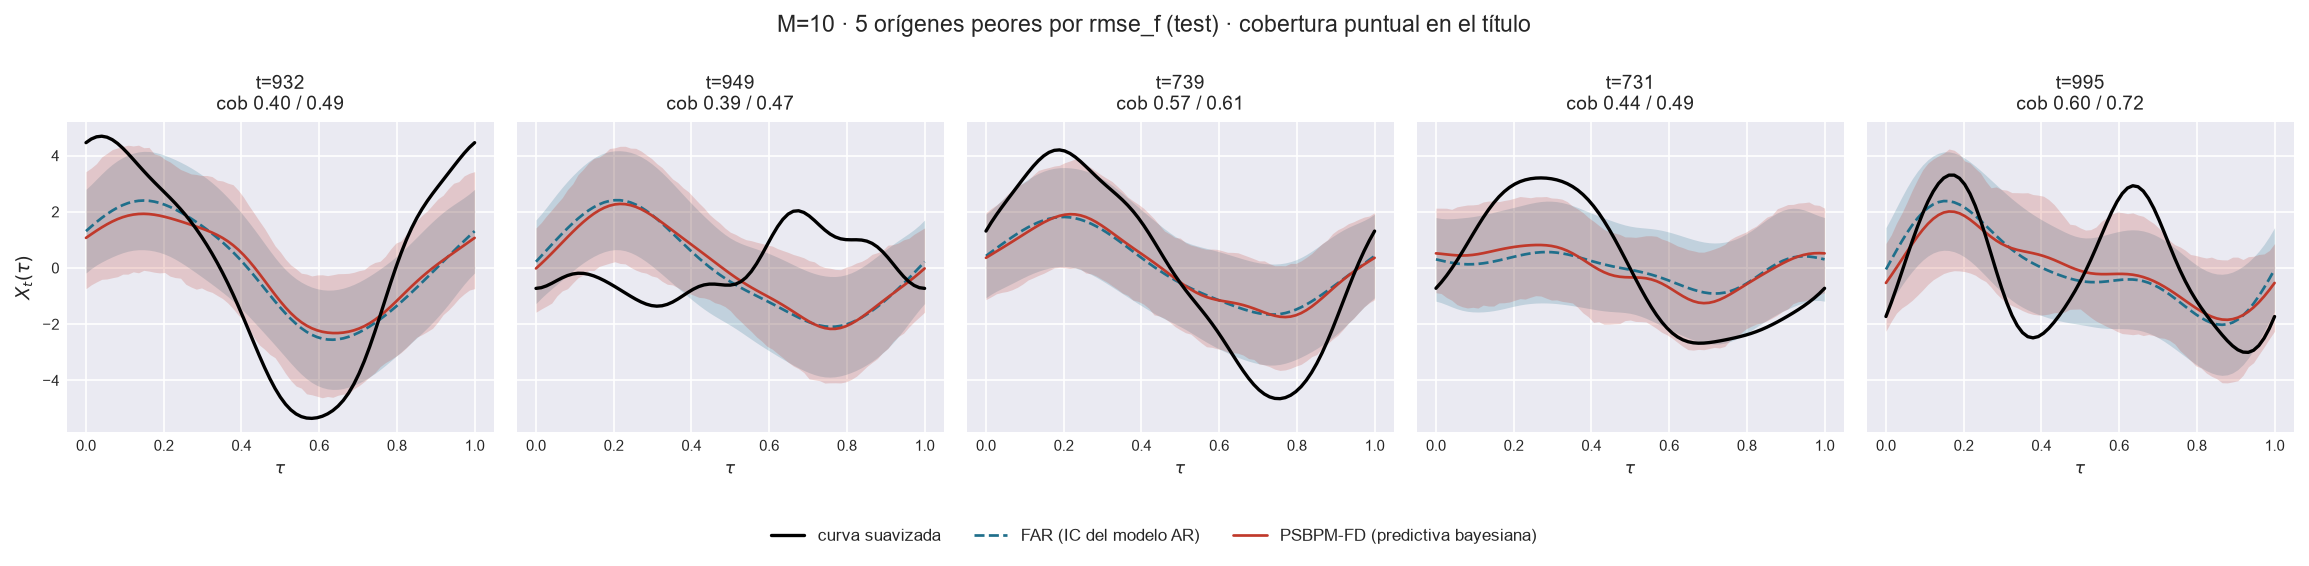
\includegraphics[width=\textwidth,height=0.45\textheight,keepaspectratio]{IMG/aneB_00/aneB_00_curvas_peo_C1.png}
\caption{C-1 (GARCH). Orígenes con peor desempeño del PSBPM-FD frente al FAR.}
\label{fig:aneB_curvas_peo_C1}
\end{figure}

\subsection{Escenario C-2 (TAR)}
\label{aneB_00_06_01_curvas_tar}

\begin{figure}[H]
\centering
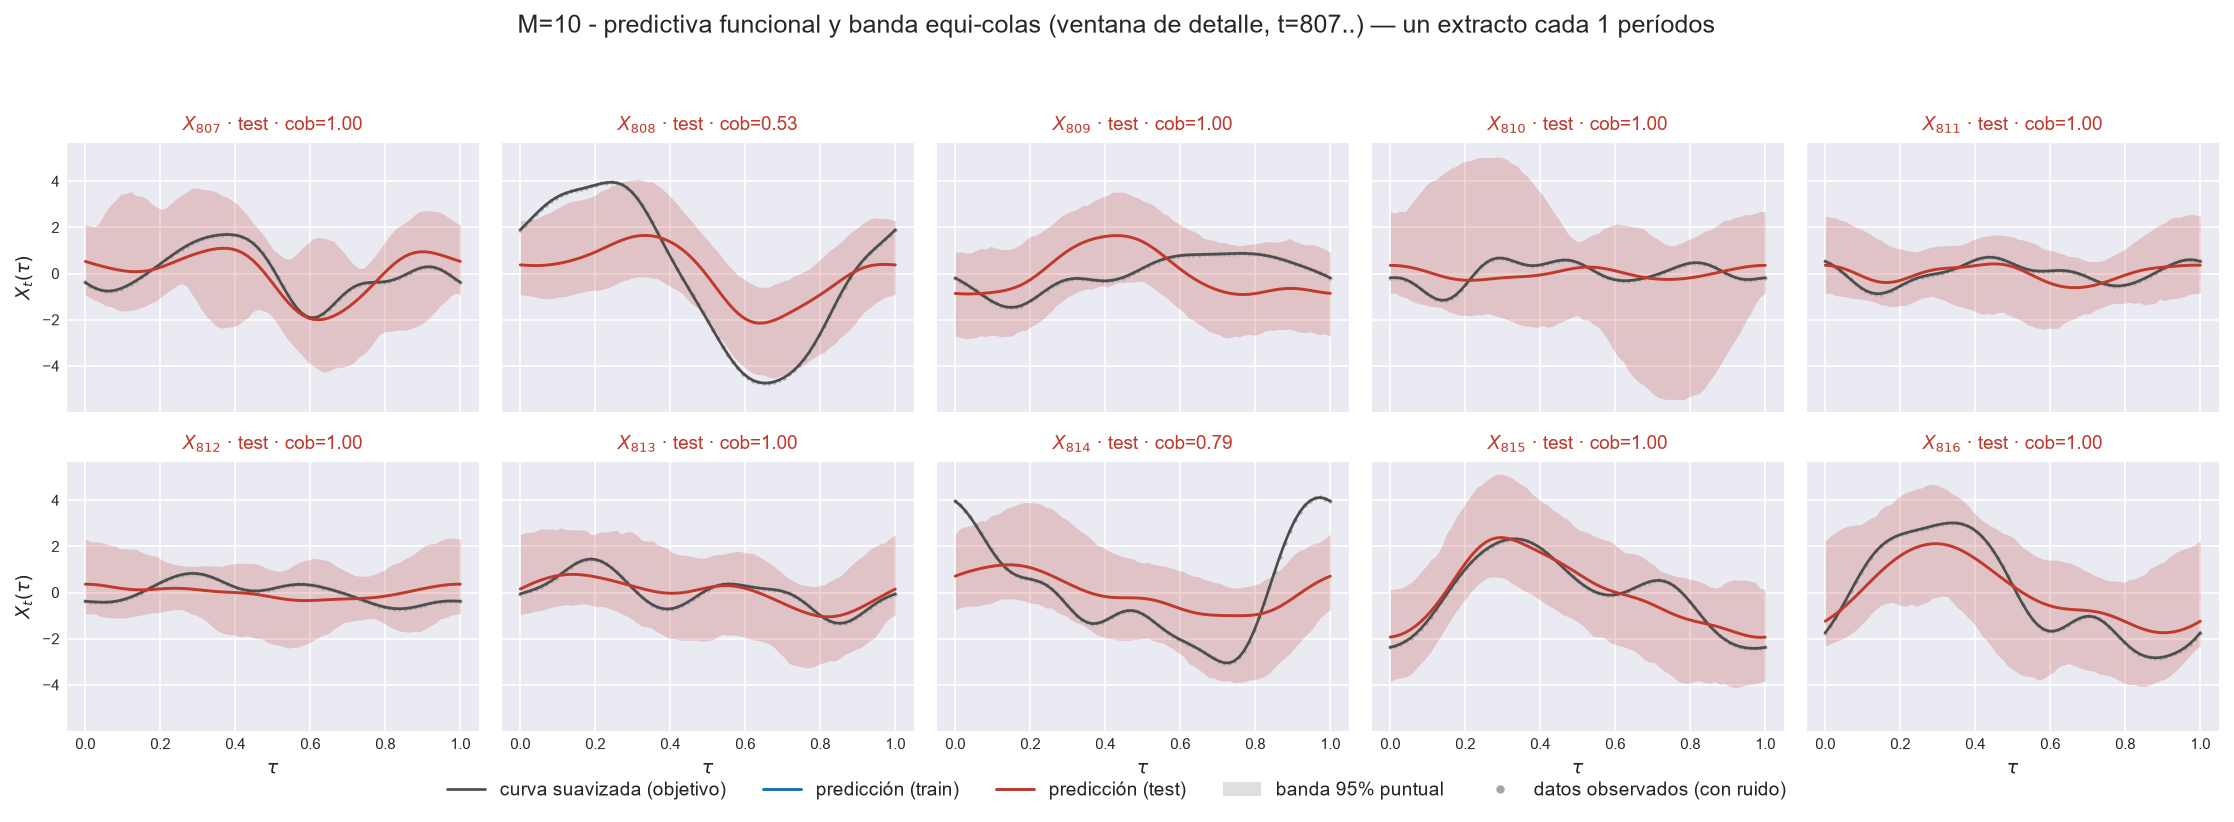
\includegraphics[width=\textwidth,height=0.45\textheight,keepaspectratio]{IMG/aneB_00/aneB_00_curvas_ext_C2.png}
\caption{C-2 (TAR). Extractos de curvas del bloque de prueba con la predicción y su banda.}
\label{fig:aneB_curvas_ext_C2}
\end{figure}

\begin{figure}[H]
\centering
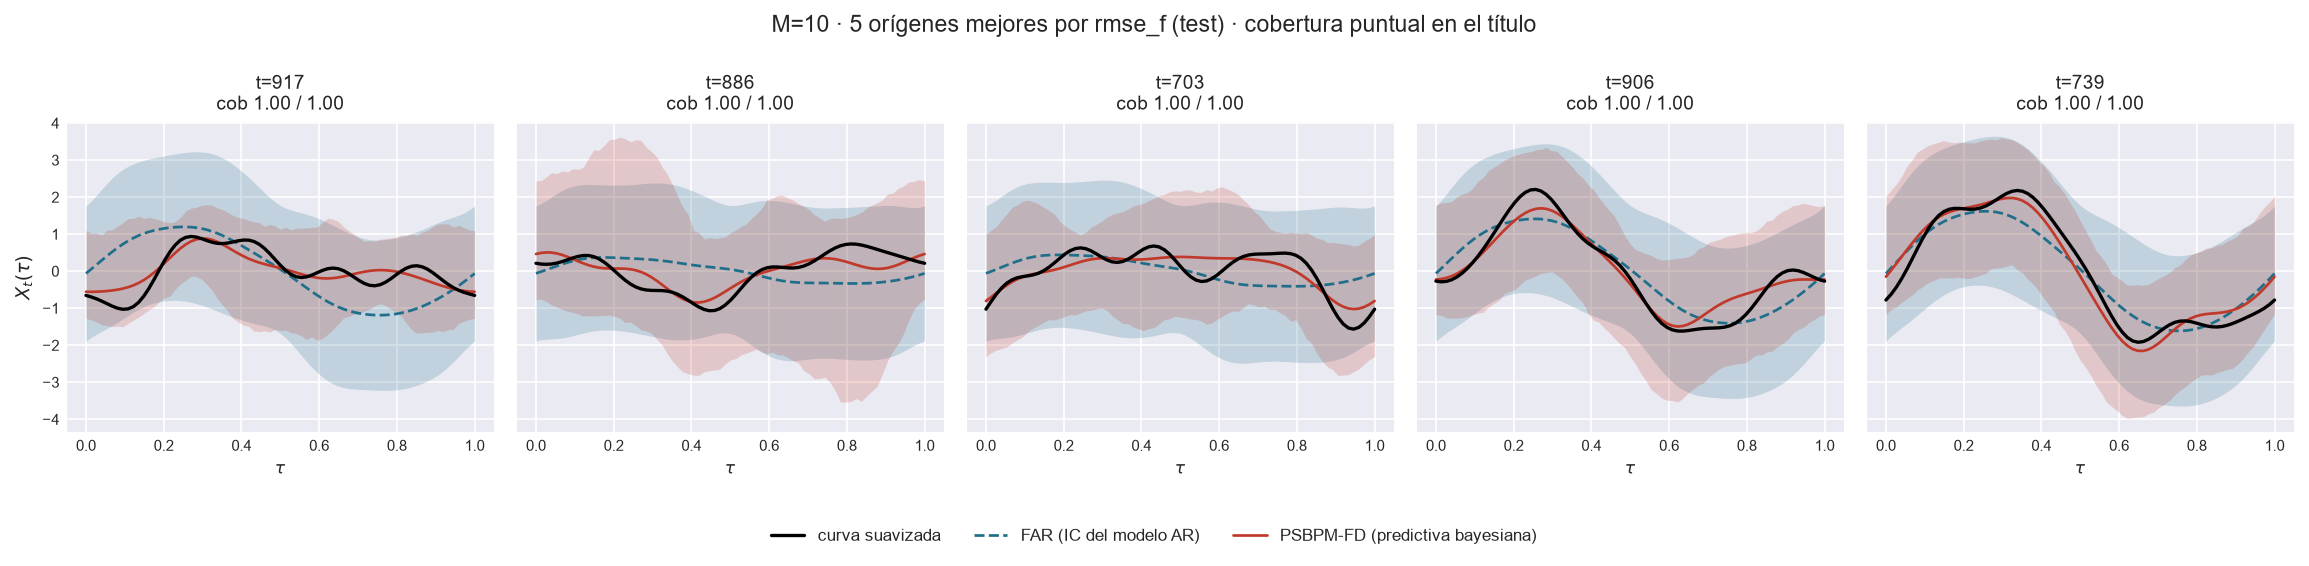
\includegraphics[width=\textwidth,height=0.45\textheight,keepaspectratio]{IMG/aneB_00/aneB_00_curvas_mej_C2.png}
\caption{C-2 (TAR). Orígenes con mejor desempeño del PSBPM-FD frente al FAR.}
\label{fig:aneB_curvas_mej_C2}
\end{figure}

\begin{figure}[H]
\centering
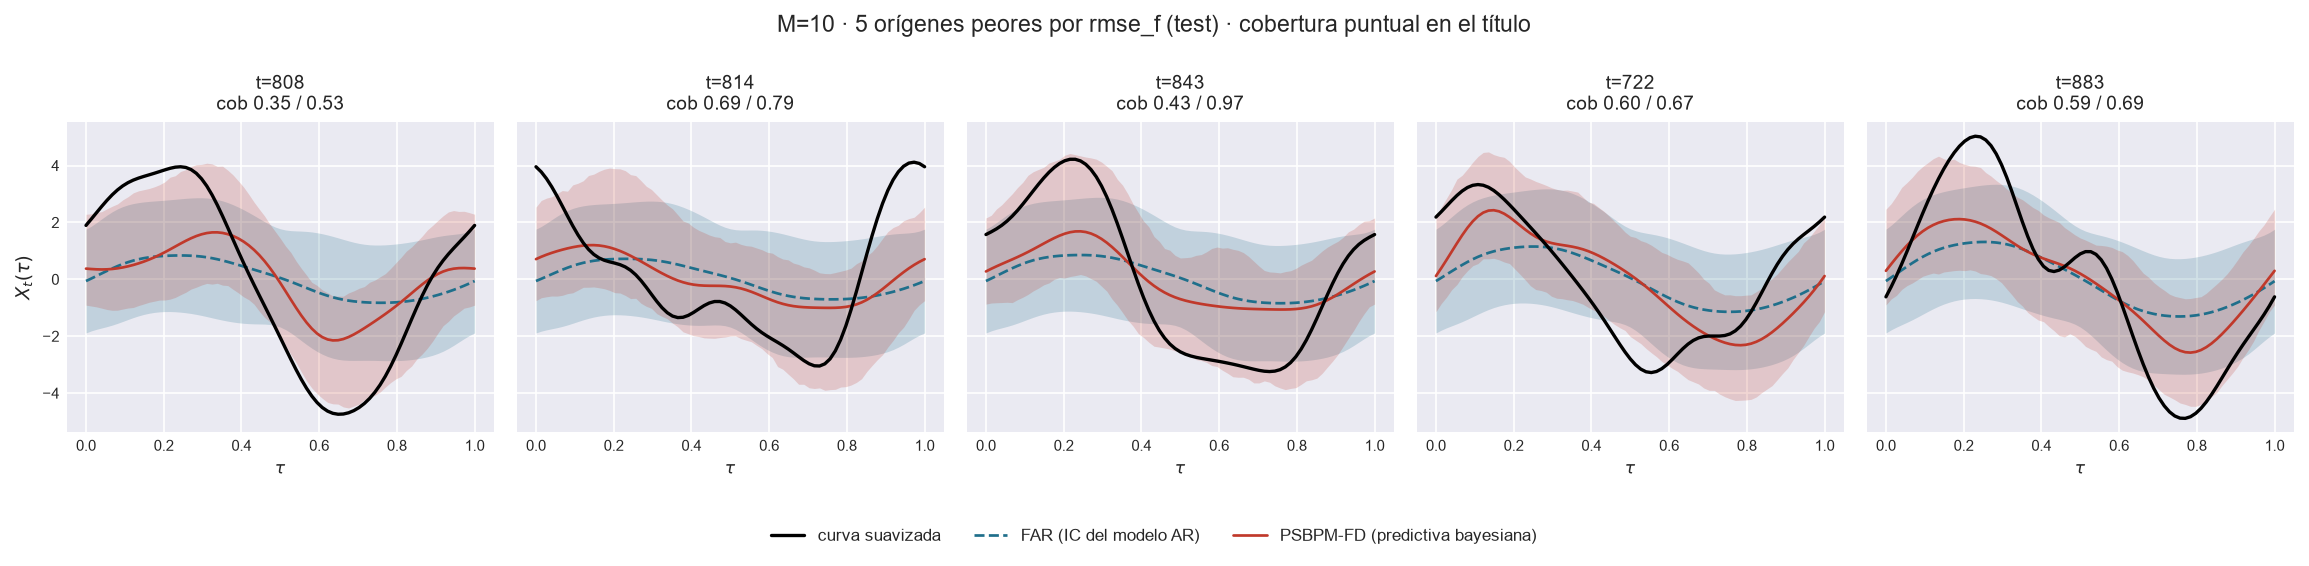
\includegraphics[width=\textwidth,height=0.45\textheight,keepaspectratio]{IMG/aneB_00/aneB_00_curvas_peo_C2.png}
\caption{C-2 (TAR). Orígenes con peor desempeño del PSBPM-FD frente al FAR.}
\label{fig:aneB_curvas_peo_C2}
\end{figure}

\subsection{Escenario C-3 (multimodalidad)}
\label{aneB_00_06_03_curvas_multimodal}

\begin{figure}[H]
\centering
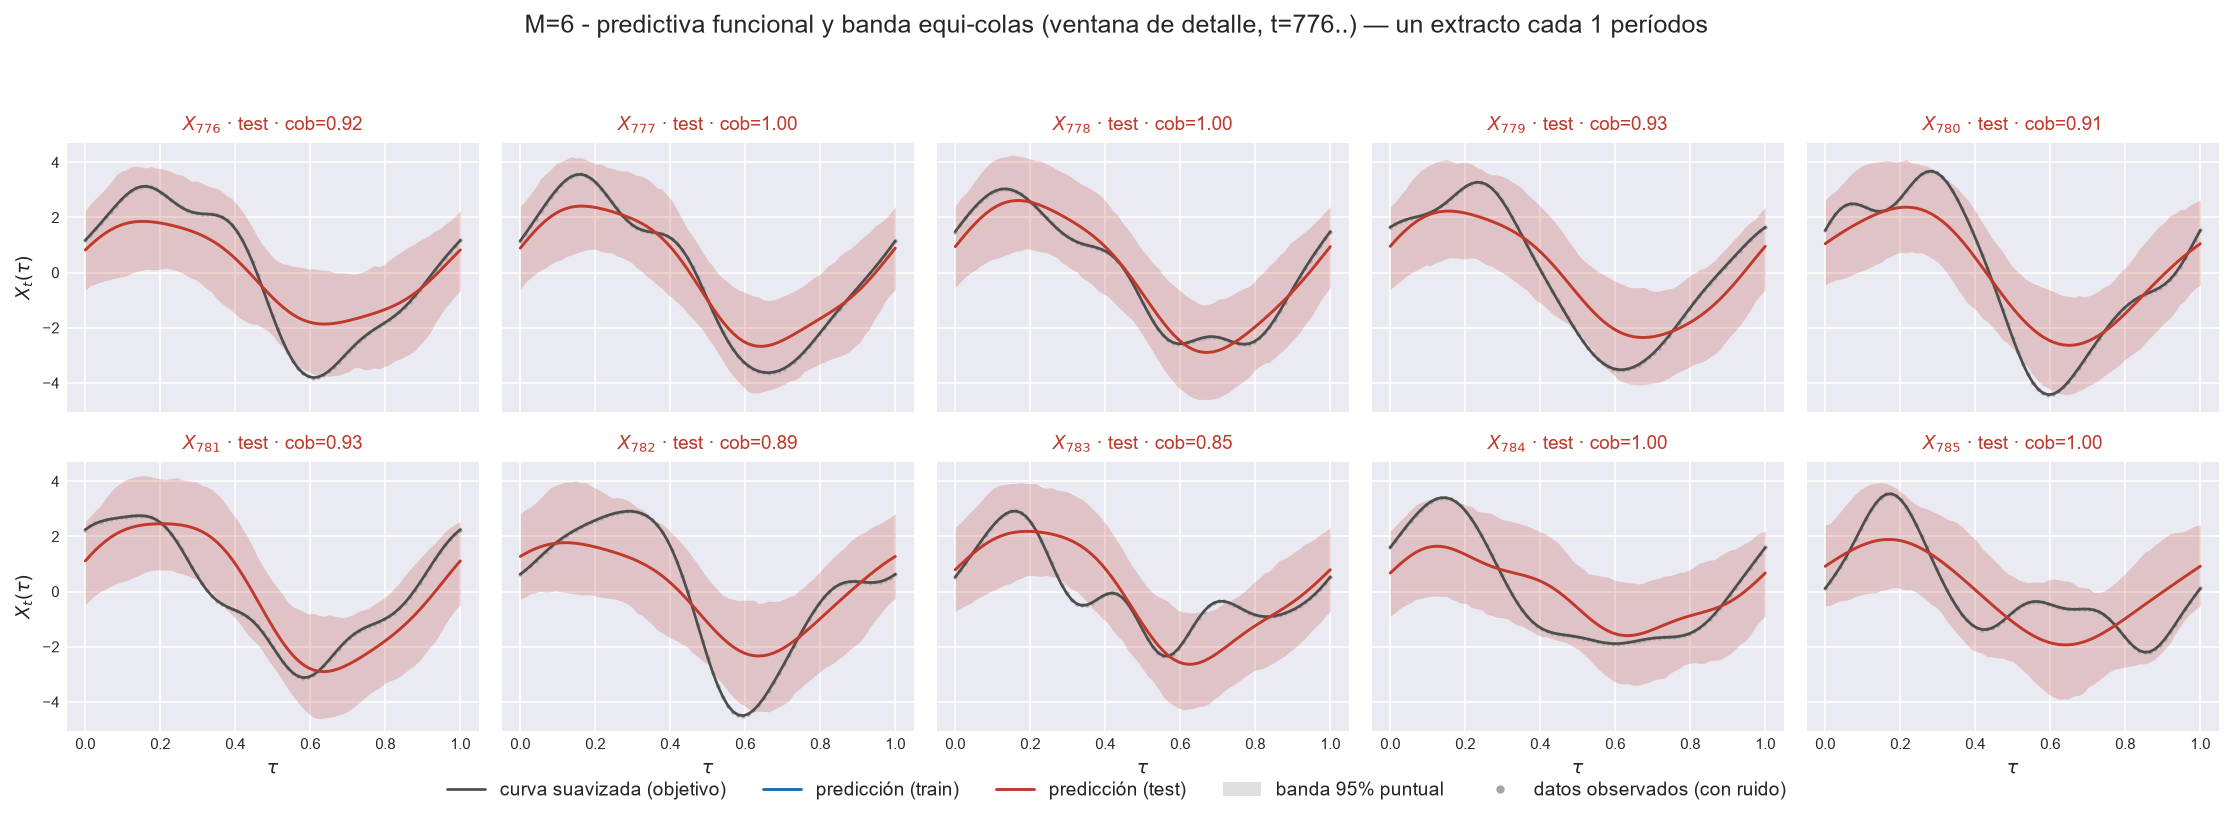
\includegraphics[width=\textwidth,height=0.45\textheight,keepaspectratio]{IMG/aneB_00/aneB_00_curvas_ext_C3.png}
\caption{C-3 (multimodalidad). Extractos de curvas del bloque de prueba con la predicción y su banda.}
\label{fig:aneB_curvas_ext_C3}
\end{figure}

\begin{figure}[H]
\centering
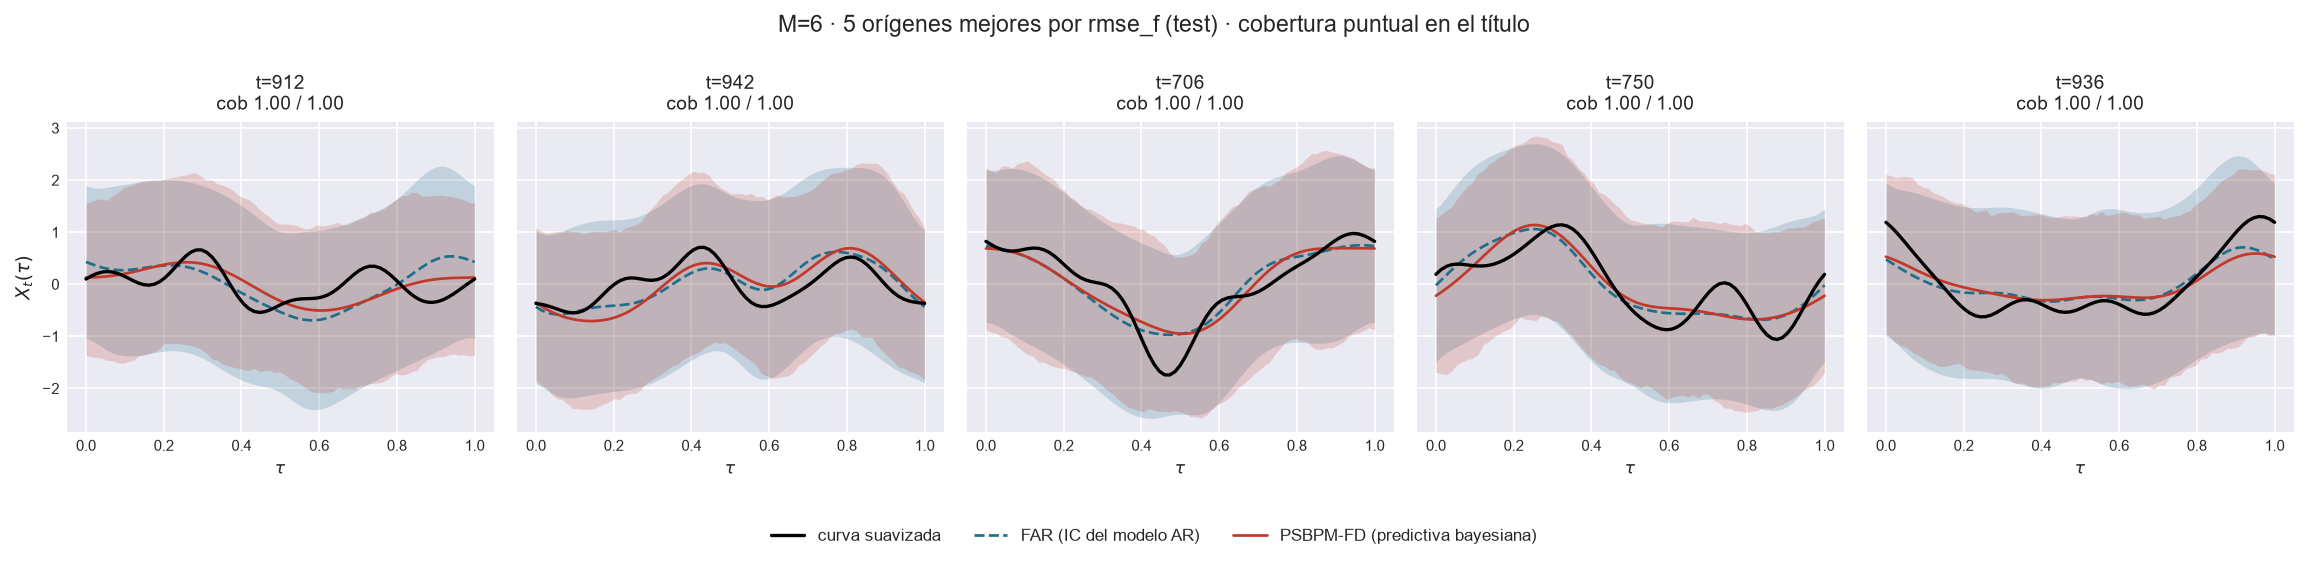
\includegraphics[width=\textwidth,height=0.45\textheight,keepaspectratio]{IMG/aneB_00/aneB_00_curvas_mej_C3.png}
\caption{C-3 (multimodalidad). Orígenes con mejor desempeño del PSBPM-FD frente al FAR.}
\label{fig:aneB_curvas_mej_C3}
\end{figure}

\begin{figure}[H]
\centering
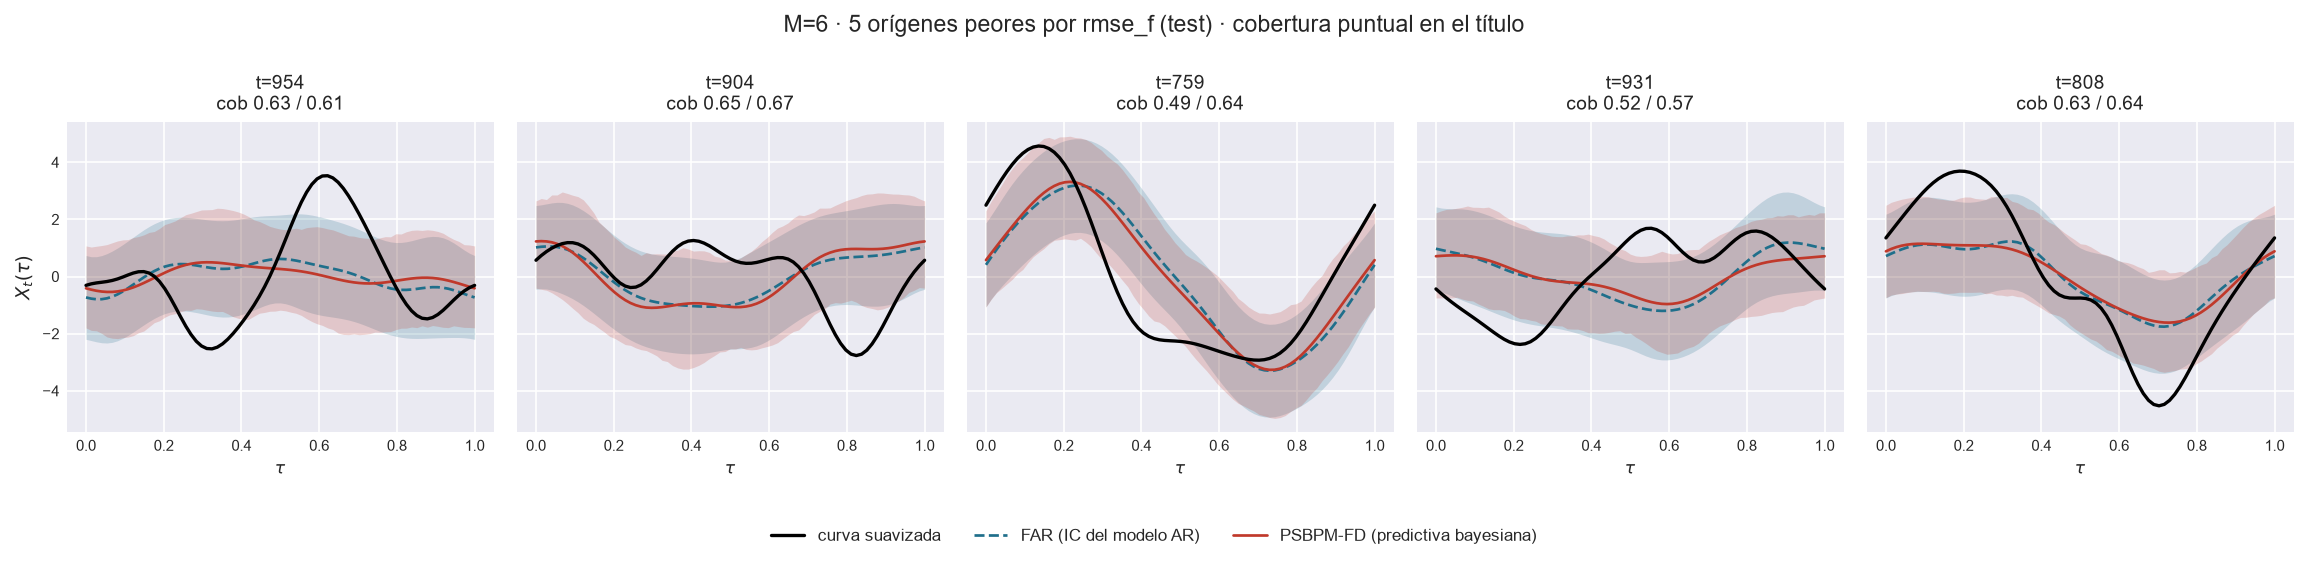
\includegraphics[width=\textwidth,height=0.45\textheight,keepaspectratio]{IMG/aneB_00/aneB_00_curvas_peo_C3.png}
\caption{C-3 (multimodalidad). Orígenes con peor desempeño del PSBPM-FD frente al FAR.}
\label{fig:aneB_curvas_peo_C3}
\end{figure}

\chapter{Resultados Complementarios de la Aplicación al Tráfico}
\label{aneC_00_00_trafico}

% Corridas 101 (rezago {1}) y 102 (rezagos {1, 7}), M = 10, test, w = 30 salvo indicación.
% Cuadros desde reports/reales/real_trafico_10{1,2}_v01_barrido_M/{98,99}_* y desde los .npz del _04;
% figuras de §3, §5 y §6 redibujadas con el estilo del Capítulo 3 (scratchpad figuras_trafico.py); el resto, del _01/_04.

Este anexo reúne los resultados de la aplicación al tráfico del Capítulo~\ref{04_00_00_aplicacion} que no se reportan en el cuerpo, para las dos especificaciones que se comparan, la que usa el rezago de un día, $\{1\}$, y la que agrega el de una semana, $\{1,7\}$. Salvo indicación, las cifras corresponden a $M = 10$, al bloque de prueba y a la ventana móvil de ancho $w = 30$.

\section{Configuración de la aplicación}
\label{aneC_00_01_configuracion}

El Cuadro~\ref{tab:aneC_configuracion} recoge la configuración con que se ajustaron las dos especificaciones. Lo que no se indica coincide con el estudio de simulación (Anexo~\ref{ane_00_03_configuracion}); las diferencias son la representación, que aquí se estima, el hiperparámetro de forma $a_\nu$, la inclusión a priori de los rezagos y el número de cadenas.

\begin{table}[H]
\centering\small
\caption{Configuración de la aplicación al tráfico.}
\label{tab:aneC_configuracion}
\begin{tabular}{p{0.22\textwidth} p{0.40\textwidth} p{0.30\textwidth}}
\hline
Elemento & Descripción & Valor \\
\hline
Datos & Metro Interstate Traffic Volume (UCI), estación ATR 301, I-94 oeste & Volumen horario, miles de veh./h \\
Ventana & Días de la serie / horas por día & 1 jul 2015 a 30 sep 2018, $T = 1188$ / $G = 24$ \\
Partición & Entrenamiento / prueba & 831 / 357 días ($T_0 = 831$) \\
Representación & B-spline cúbica ajustada a las horas observadas & $J = 10$ \\
FPCA & Componentes retenidas, estimadas en entrenamiento & $M = 10$ \\
Covariables & Scores de $t-1$ / de $t-1$ y $t-7$ & $d = 10$ / $d = 20$ \\
$N$, $L_j$ & Truncamiento y grilla de localización & $30$, $50$ \\
Muestreador & Cadenas / iteraciones / descartadas & $1$ / $2500$ / $1000$ \\
$a_\nu$, $a_\varkappa$, $b_\varkappa$ & Forma de las precisiones y de la contracción & $2$, $0.5$, $0.5$ \\
$(a_{\varpi_j}, b_{\varpi_j})$ & Inclusión, todos los rezagos & $(1, 5)$ \\
FAR($p$) & Orden igual al mayor rezago & $p = 1$ / $p = 7$ \\
Random Forest & Rezagos elegidos con el entrenamiento & Entre $\{1\}$ y $\{1,7\}$ \\
Ventana de detalle & Diez días con más días no laborables & 23 dic 2017 a 1 ene 2018 ($t = 907$ a $916$) \\
\hline
\end{tabular}
\end{table}

Las constantes de los comportamientos son las del Cuadro~\ref{tab:dis_comportamientos}, sin recorte de las extracciones, porque con $a_\nu = 2$ la varianza de los átomos es finita.

\section{Datos y representación}
\label{aneC_00_02_datos}
% Mismos días en 101 y 102: figuras de la 102_01 (01-10).

La serie diaria, sus momentos, la representación en la base B-spline y la FPCA son comunes a las dos especificaciones.

\begin{figure}[H]
\centering
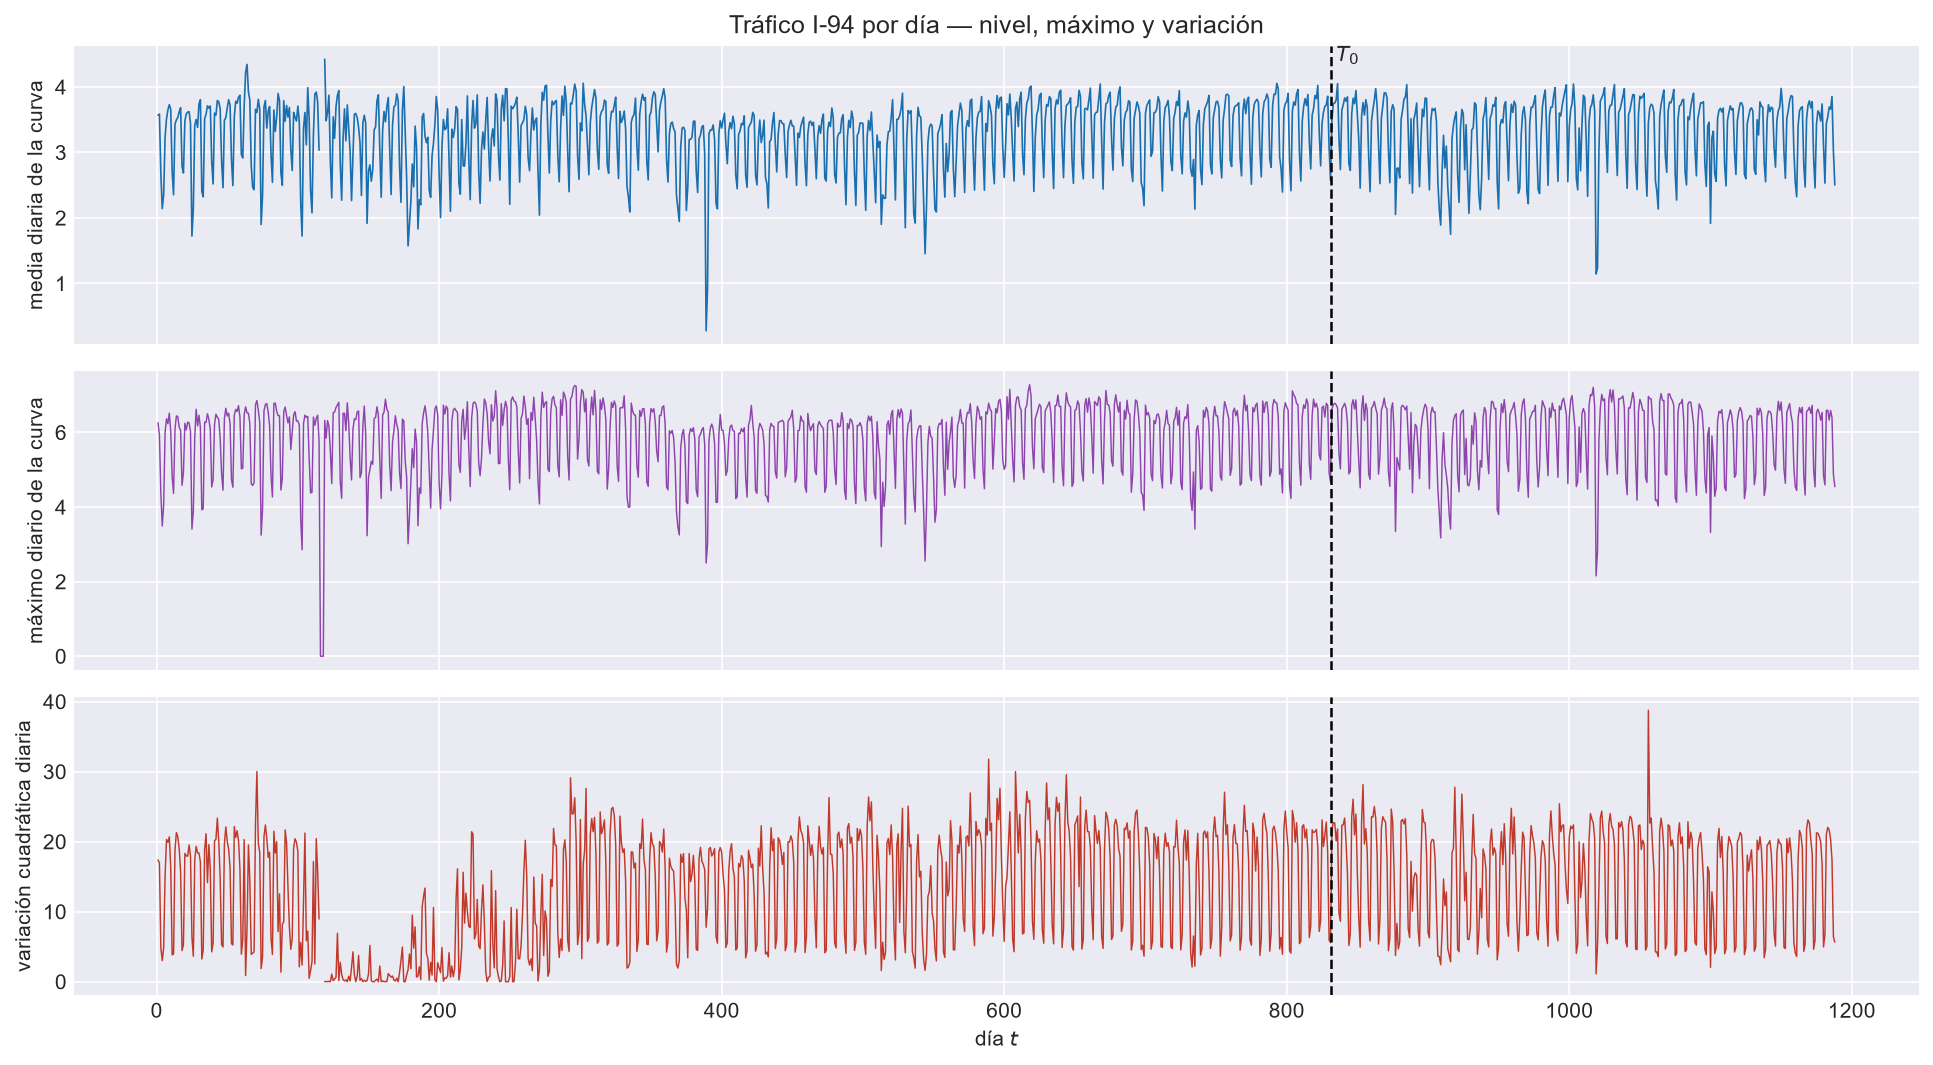
\includegraphics[width=\textwidth,height=0.7\textheight,keepaspectratio]{IMG/aneC_00/aneC_00_04_serie_diaria.png}
\caption{Serie diaria del volumen de tráfico.}
\label{fig:aneC_04_serie_diaria}
\end{figure}

\begin{figure}[H]
\centering
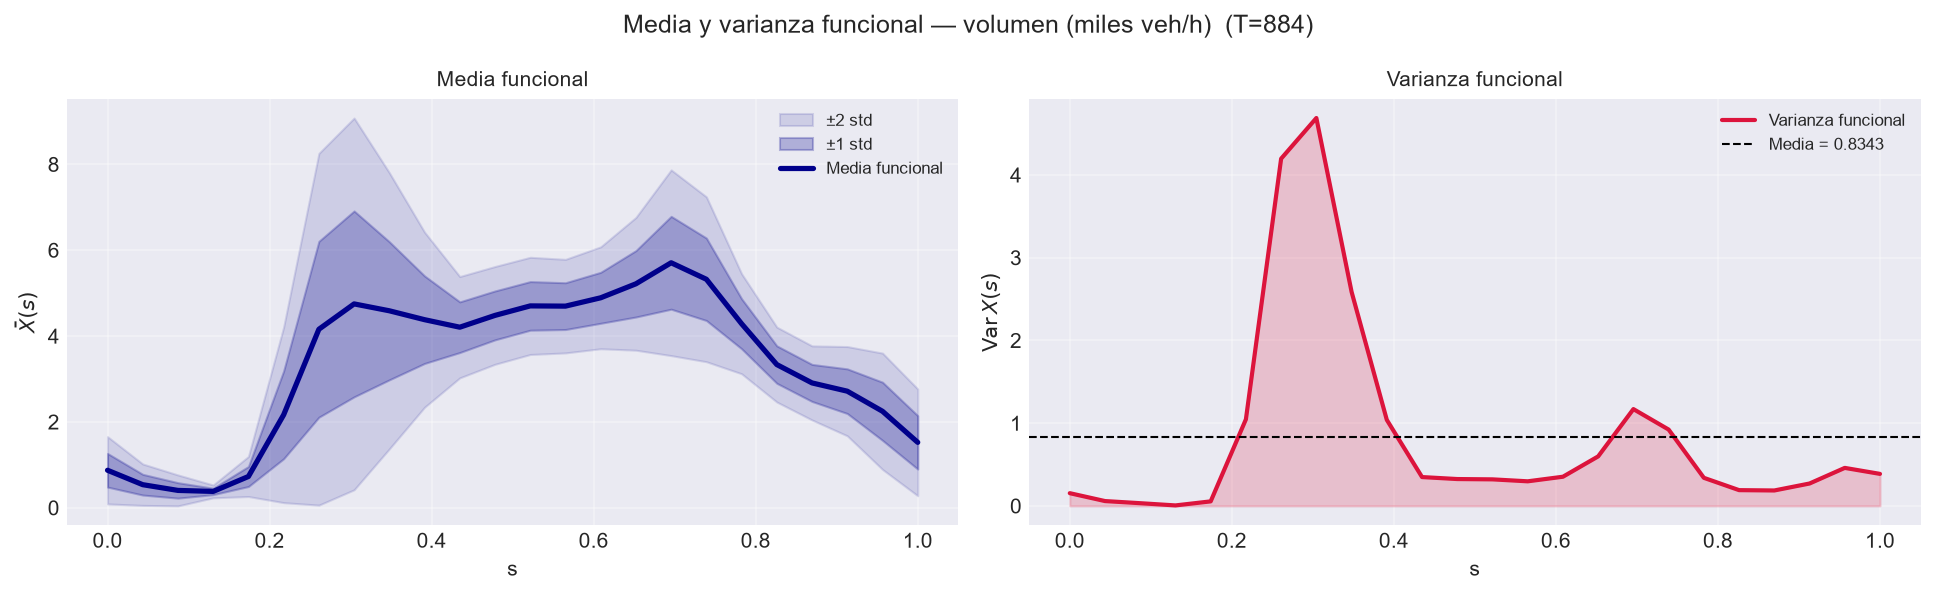
\includegraphics[width=\textwidth,height=0.7\textheight,keepaspectratio]{IMG/aneC_00/aneC_00_03_media_varianza_raw.png}
\caption{Media y varianza de la curva diaria.}
\label{fig:aneC_03_media_varianza_raw}
\end{figure}

\begin{figure}[H]
\centering
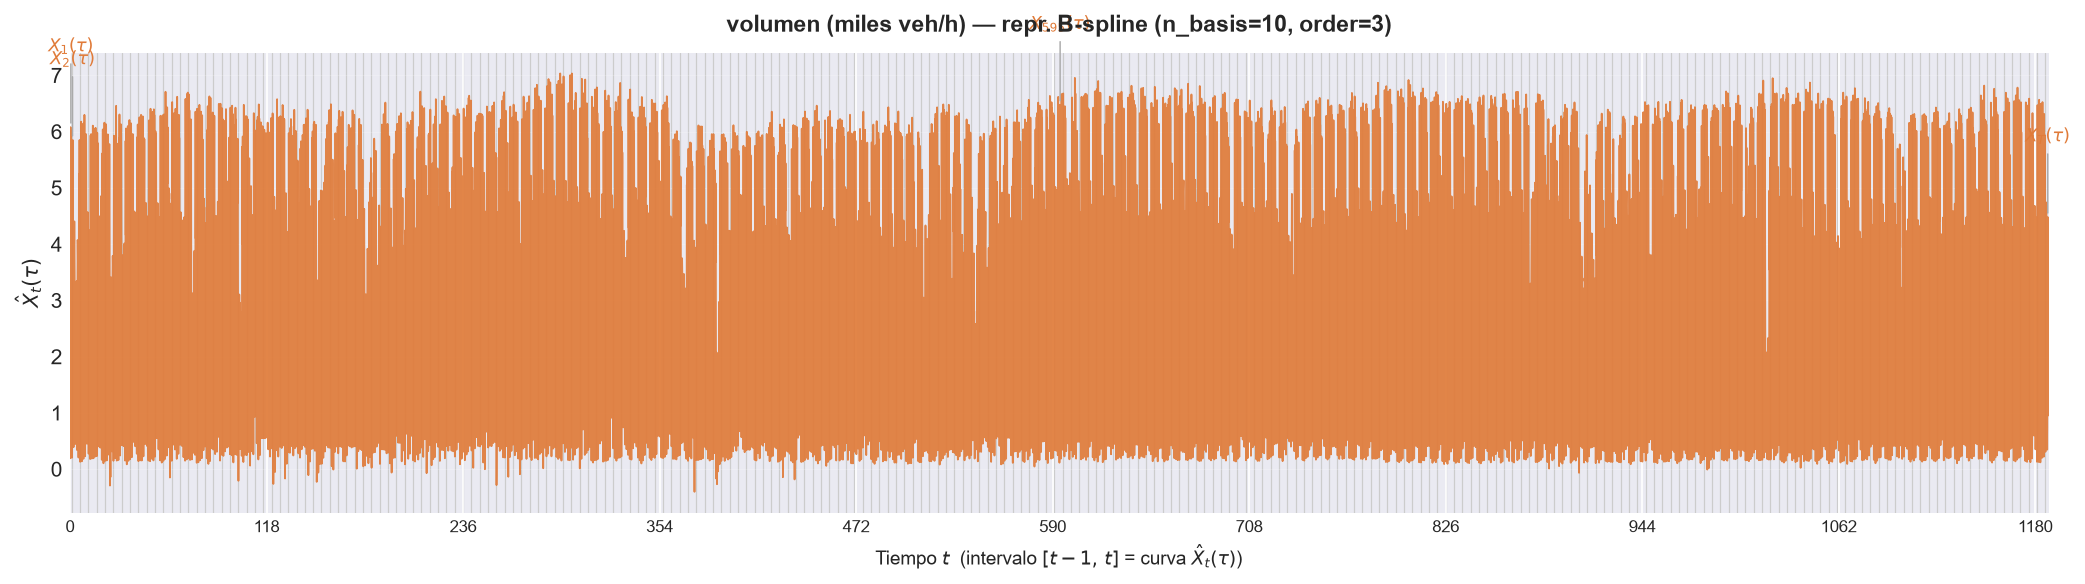
\includegraphics[width=\textwidth,height=0.7\textheight,keepaspectratio]{IMG/aneC_00/aneC_00_06_fts_funcional_bspline.png}
\caption{Curvas diarias en la base B-spline con $J = 10$.}
\label{fig:aneC_06_fts_funcional_bspline}
\end{figure}

\begin{figure}[H]
\centering
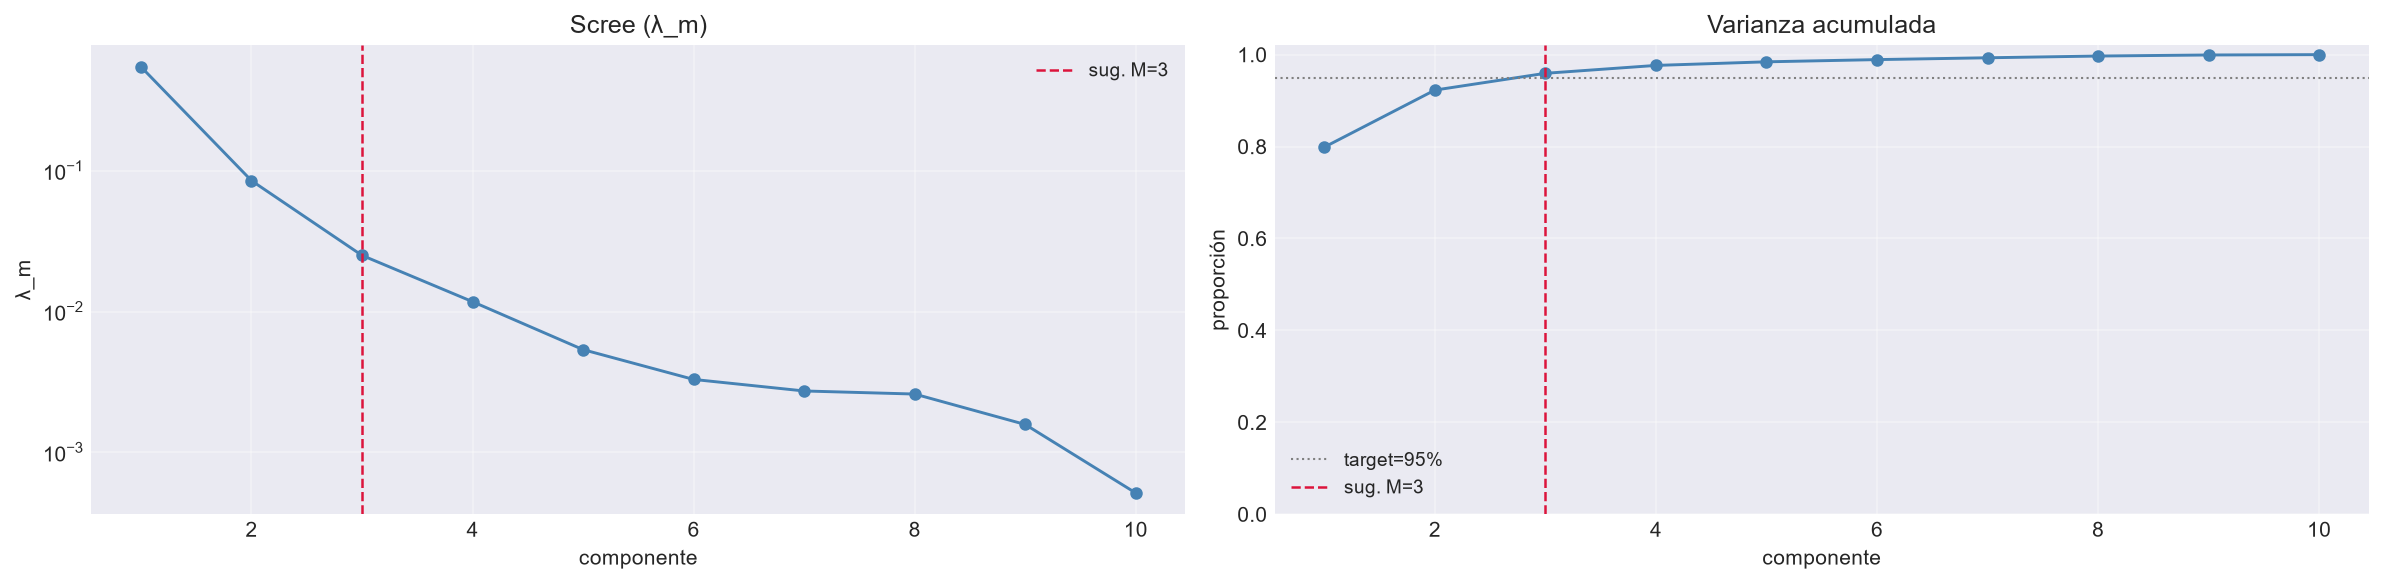
\includegraphics[width=\textwidth,height=0.7\textheight,keepaspectratio]{IMG/aneC_00/aneC_00_07_fpca_scree.png}
\caption{Varianza explicada por componente de la FPCA (bloque de entrenamiento).}
\label{fig:aneC_07_fpca_scree}
\end{figure}

\begin{figure}[H]
\centering
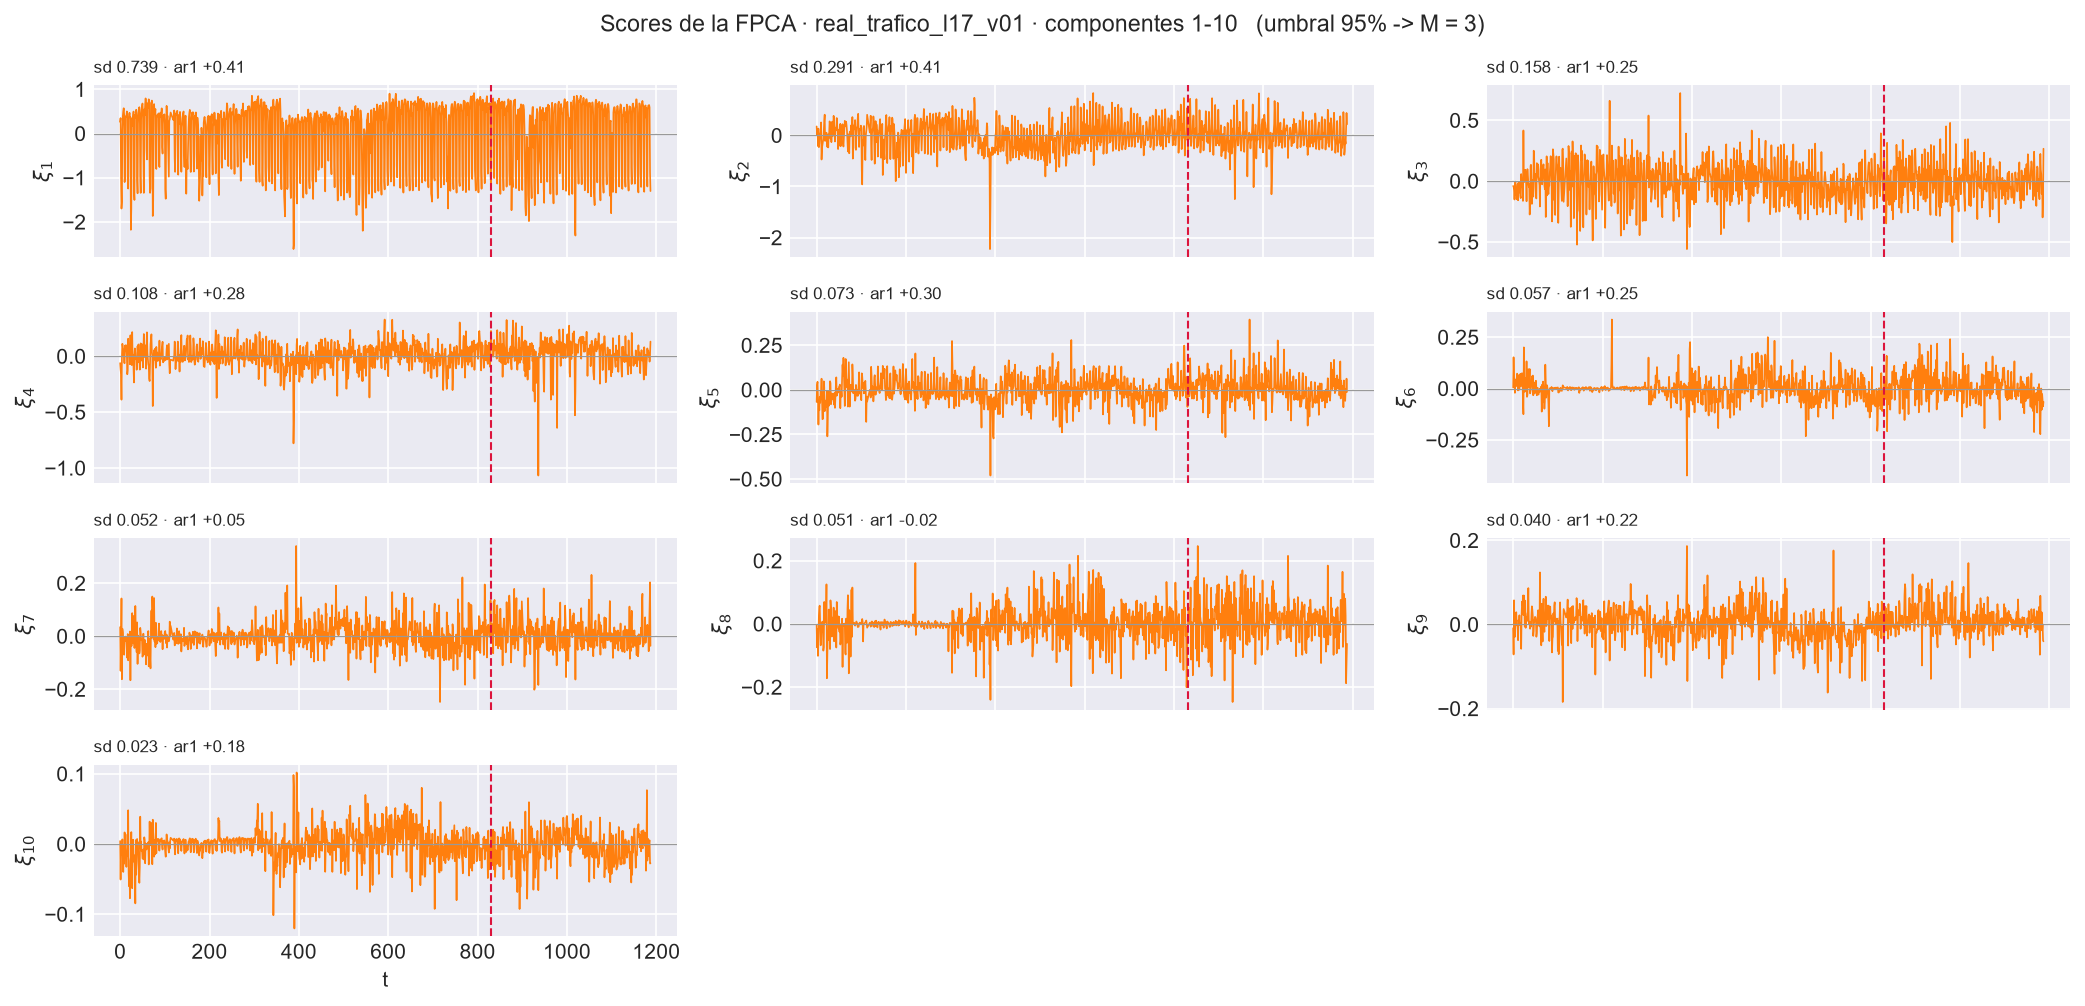
\includegraphics[width=\textwidth,height=0.7\textheight,keepaspectratio]{IMG/aneC_00/aneC_00_07b_series_scores.png}
\caption{Series de scores de la FPCA.}
\label{fig:aneC_07b_series_scores}
\end{figure}

\begin{figure}[H]
\centering
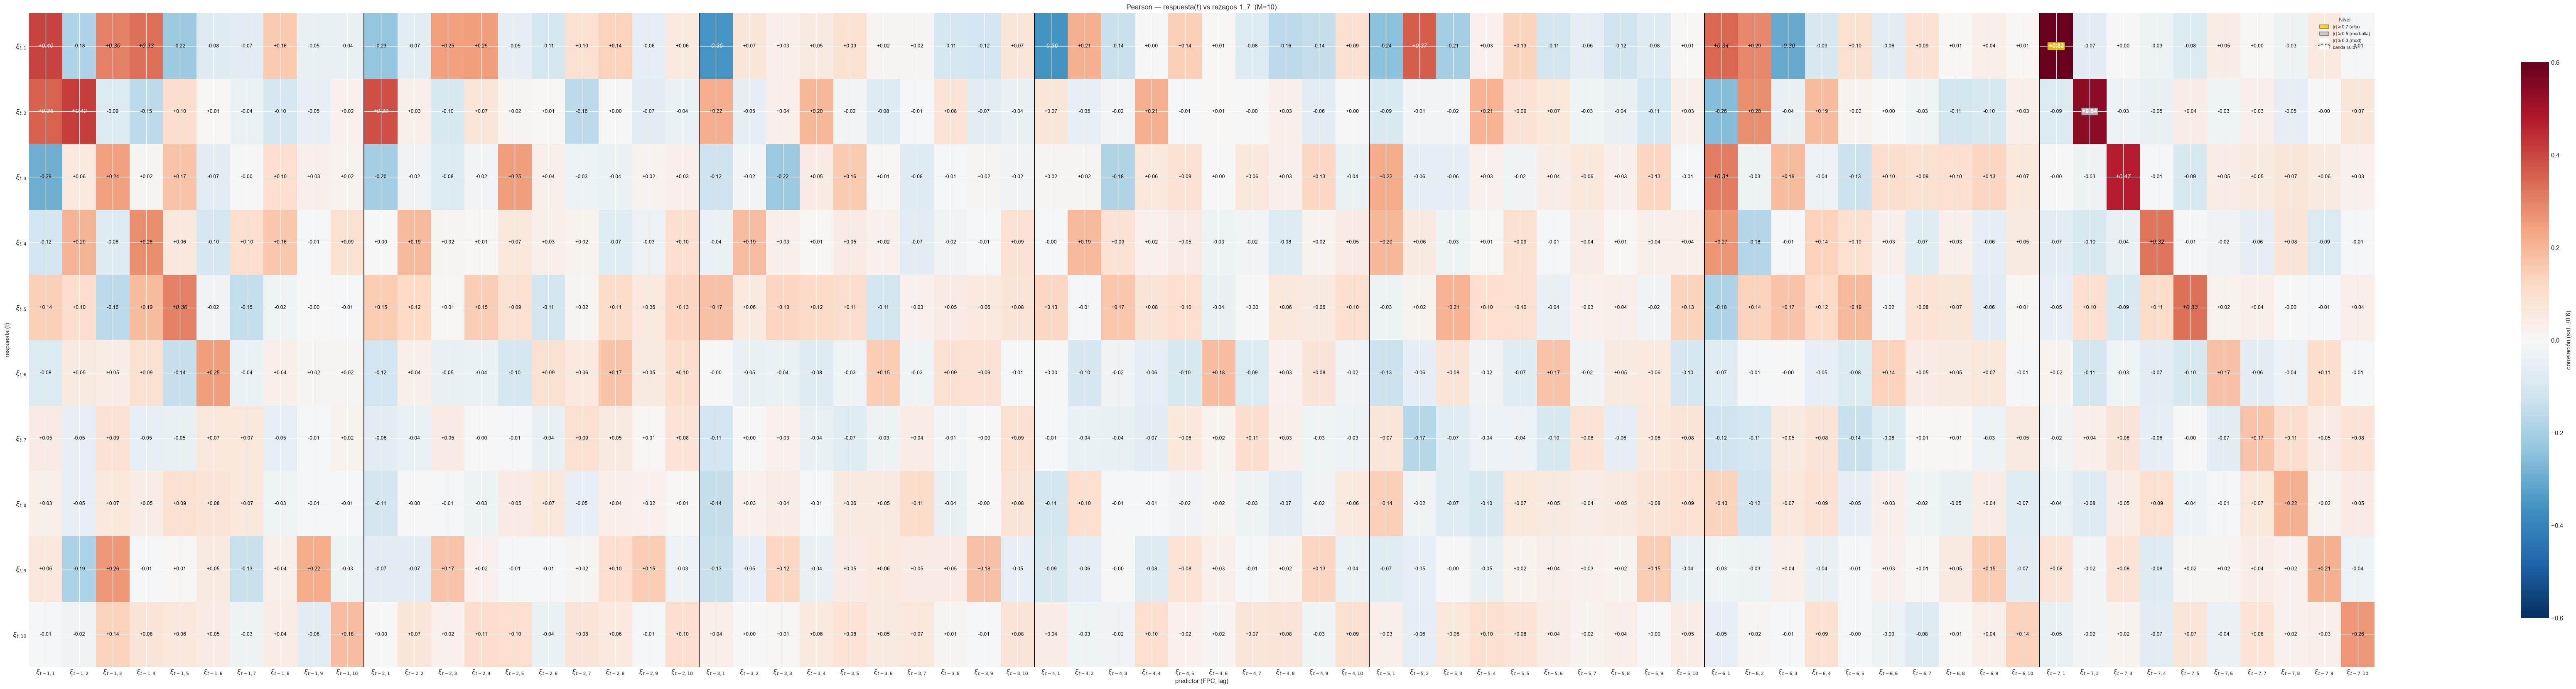
\includegraphics[width=\textwidth,height=0.7\textheight,keepaspectratio]{IMG/aneC_00/aneC_00_09a_rezagos_pearson.png}
\caption{Autocorrelación de los scores por rezago (Pearson).}
\label{fig:aneC_09a_rezagos_pearson}
\end{figure}

\begin{figure}[H]
\centering
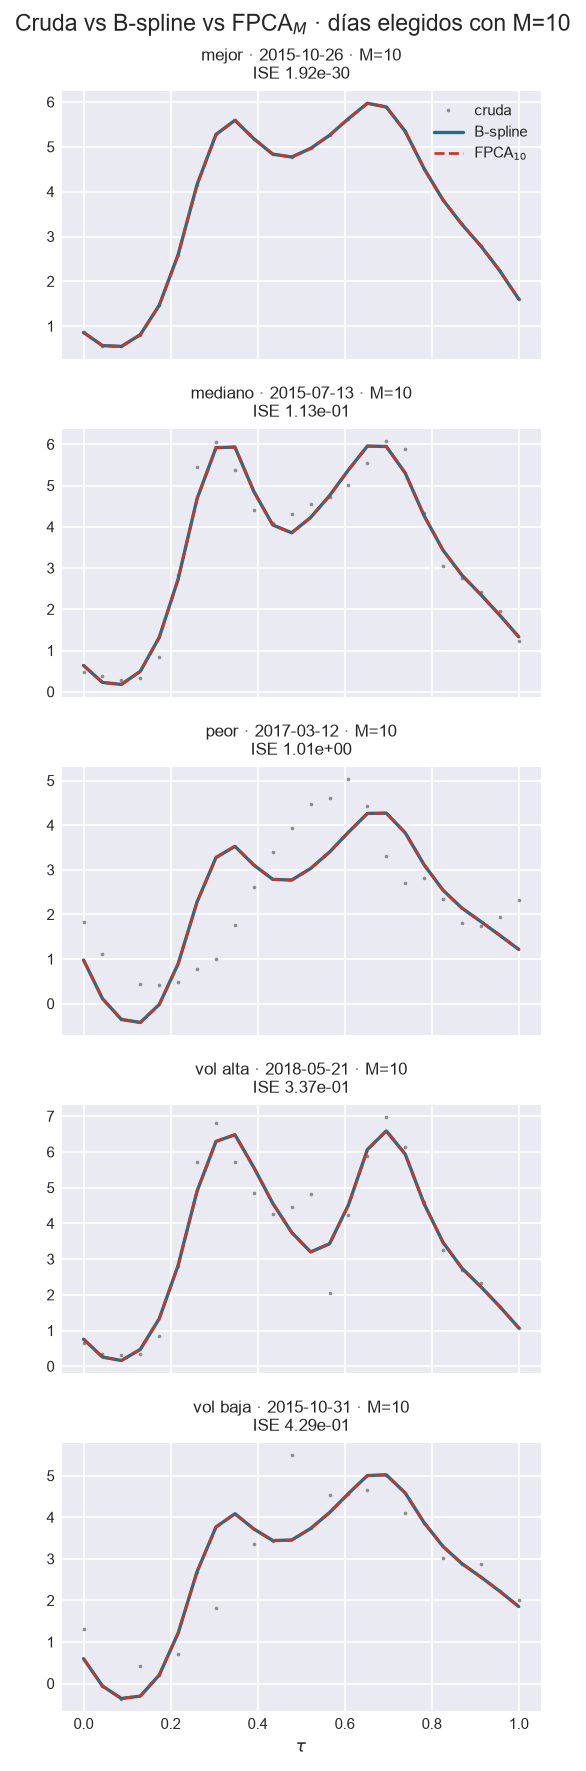
\includegraphics[width=\textwidth,height=0.7\textheight,keepaspectratio]{IMG/aneC_00/aneC_00_10_tres_curvas.png}
\caption{Tres curvas observadas y su representación con $M = 10$.}
\label{fig:aneC_10_tres_curvas}
\end{figure}

\section{Métricas completas}
\label{aneC_00_03_metricas}

Las diez métricas del Marco Teórico en el bloque de prueba, como promedio sobre las ventanas de ancho $w = 30$.
% Fuente: 98_resumen_bloqueA_min_max_prom.csv de 101 y 102 (test, M = 10).
\begin{table}[H]
\centering\small
\caption{Métricas de error en el bloque de prueba del tráfico ($M = 10$, $w = 30$).}
\label{tab:aneC_A}
\begin{tabular}{l l cccc}
\hline
Rezagos & Modelo & MAE & RMSE & $\overline{\mathrm{E}}_{\max}$ & $\mathrm{E}_{\max}^{\mathrm{glob}}$ \\
\hline
$\{1\}$   & PSBPM-FD, esperanza          & 0.413 & 0.646 & 1.241 & 3.347 \\
          & PSBPM-FD, mediana puntual    & 0.376 & 0.658 & 1.147 & 3.999 \\
          & PSBPM-FD, átomo más probable & 0.397 & 0.729 & 1.198 & 4.385 \\
          & FAR                          & 0.398 & 0.621 & 1.224 & 3.102 \\
          & Random Forest                & 0.361 & 0.562 & 1.076 & 3.000 \\
\hline
$\{1,7\}$ & PSBPM-FD, esperanza          & 0.315 & 0.522 & 0.906 & 3.367 \\
          & PSBPM-FD, mediana puntual    & 0.302 & 0.528 & 0.879 & 3.628 \\
          & PSBPM-FD, átomo más probable & 0.317 & 0.556 & 0.920 & 3.859 \\
          & FAR                          & 0.314 & 0.495 & 0.897 & 3.106 \\
          & Random Forest                & 0.314 & 0.499 & 0.896 & 3.076 \\
\hline
\end{tabular}
\end{table}

% Fuente: 99_resumen_bloqueB_min_max_prom.csv de 101 y 102 (test, M = 10).
\begin{table}[H]
\centering\small
\setlength{\tabcolsep}{4pt}
\caption{Métricas de intervalo en el bloque de prueba del tráfico ($M = 10$, $w = 30$). Nivel nominal $0.95$.}
\label{tab:aneC_B}
\begin{tabular}{l l cccccc}
\hline
Rezagos & Banda & MPIW & PICP & PICPB & Winkler & $\overline{\mathrm{W}}_{\max}$ & $\mathrm{W}_{\max}^{\mathrm{glob}}$ \\
\hline
$\{1\}$   & Equi-colas      & 2.124 & 0.961 & 0.731 & 2.734 & 7.845 & 43.392 \\
          & Máxima densidad & 1.995 & 0.960 & 0.742 & 2.669 & 7.422 & 46.019 \\
          & Simultánea      & 4.242 & 0.991 & 0.942 & 4.493 & 9.717 & 33.688 \\
          & FAR             & 2.159 & 0.950 & 0.721 & 3.073 & 9.253 & 50.983 \\
\hline
$\{1,7\}$ & Equi-colas      & 1.752 & 0.956 & 0.754 & 2.707 & 8.041 & 67.843 \\
          & Máxima densidad & 1.689 & 0.955 & 0.746 & 2.714 & 7.918 & 70.530 \\
          & Simultánea      & 3.011 & 0.983 & 0.917 & 3.549 & 7.831 & 55.352 \\
          & FAR             & 1.602 & 0.930 & 0.675 & 3.052 & 9.922 & 78.072 \\
\hline
\end{tabular}
\end{table}

\begin{figure}[H]
\centering
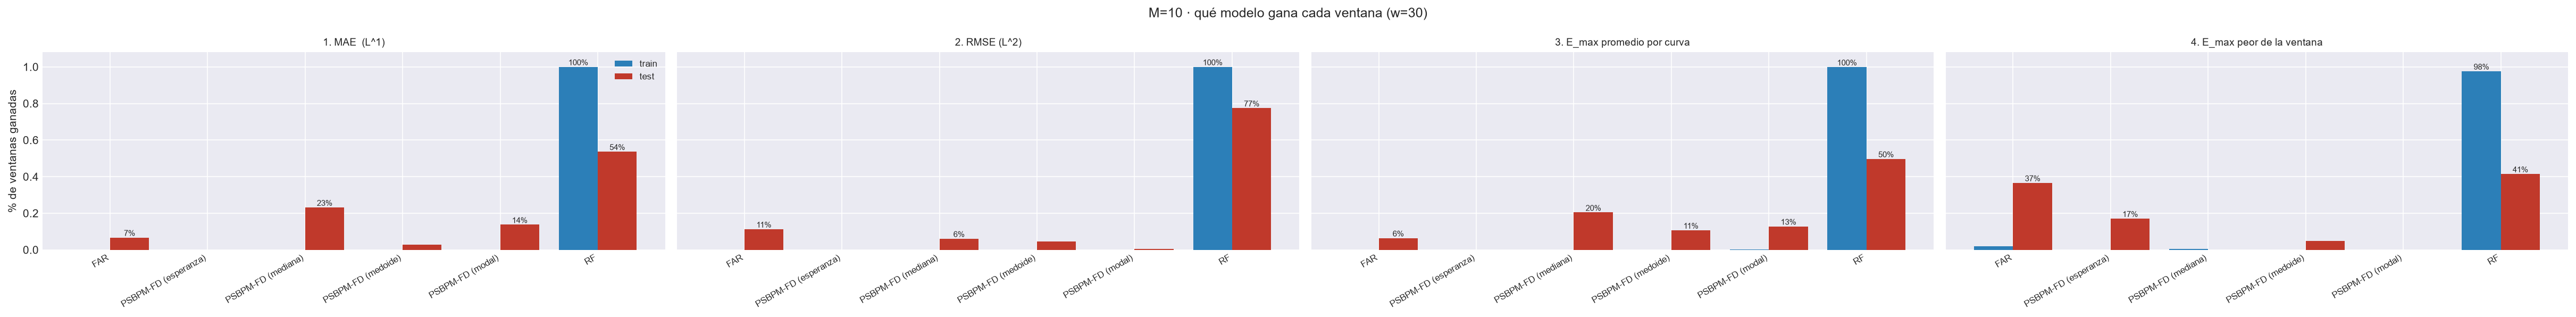
\includegraphics[width=\textwidth,height=0.75\textheight,keepaspectratio]{IMG/aneC_00/aneC_00_78_ganador_ventana_bloqueA_101.png}
\caption{Modelo con menor MAE en cada ventana, tráfico con rezago $\{1\}$ ($M = 10$).}
\label{fig:aneC_78_ganador_ventana_bloqueA_101}
\end{figure}

\begin{figure}[H]
\centering
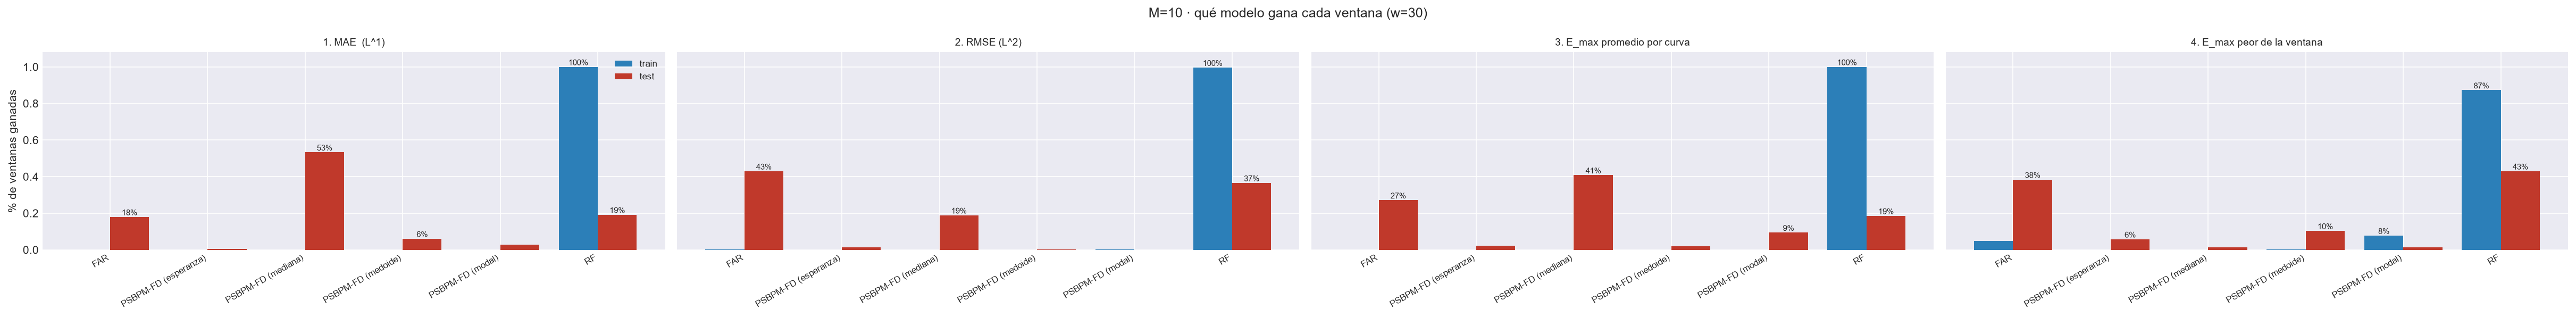
\includegraphics[width=\textwidth,height=0.75\textheight,keepaspectratio]{IMG/aneC_00/aneC_00_78_ganador_ventana_bloqueA_102.png}
\caption{Modelo con menor MAE en cada ventana, tráfico con rezagos $\{1,7\}$ ($M = 10$).}
\label{fig:aneC_78_ganador_ventana_bloqueA_102}
\end{figure}

\section{Sensibilidad al ancho de la ventana}
\label{aneC_00_04_ventana}

Las métricas de error y de intervalo sobre la ventana móvil con $w = 20$ y $w = 40$; el Capítulo~\ref{04_00_00_aplicacion} reporta $w = 30$. Las métricas de intervalo se muestran para las tres construcciones del PSBPM-FD.

% Fuente: 72_ventana_modelos_w{20,40}.csv del _05 y ventana móvil de las bandas de banda_funcional_psbp.npz,
% recalculada con la llamada del _04 (con w = 30 reproduce 81_ventana_bloqueB_w30.csv a 1e-14).
\begin{figure}[H]
\centering
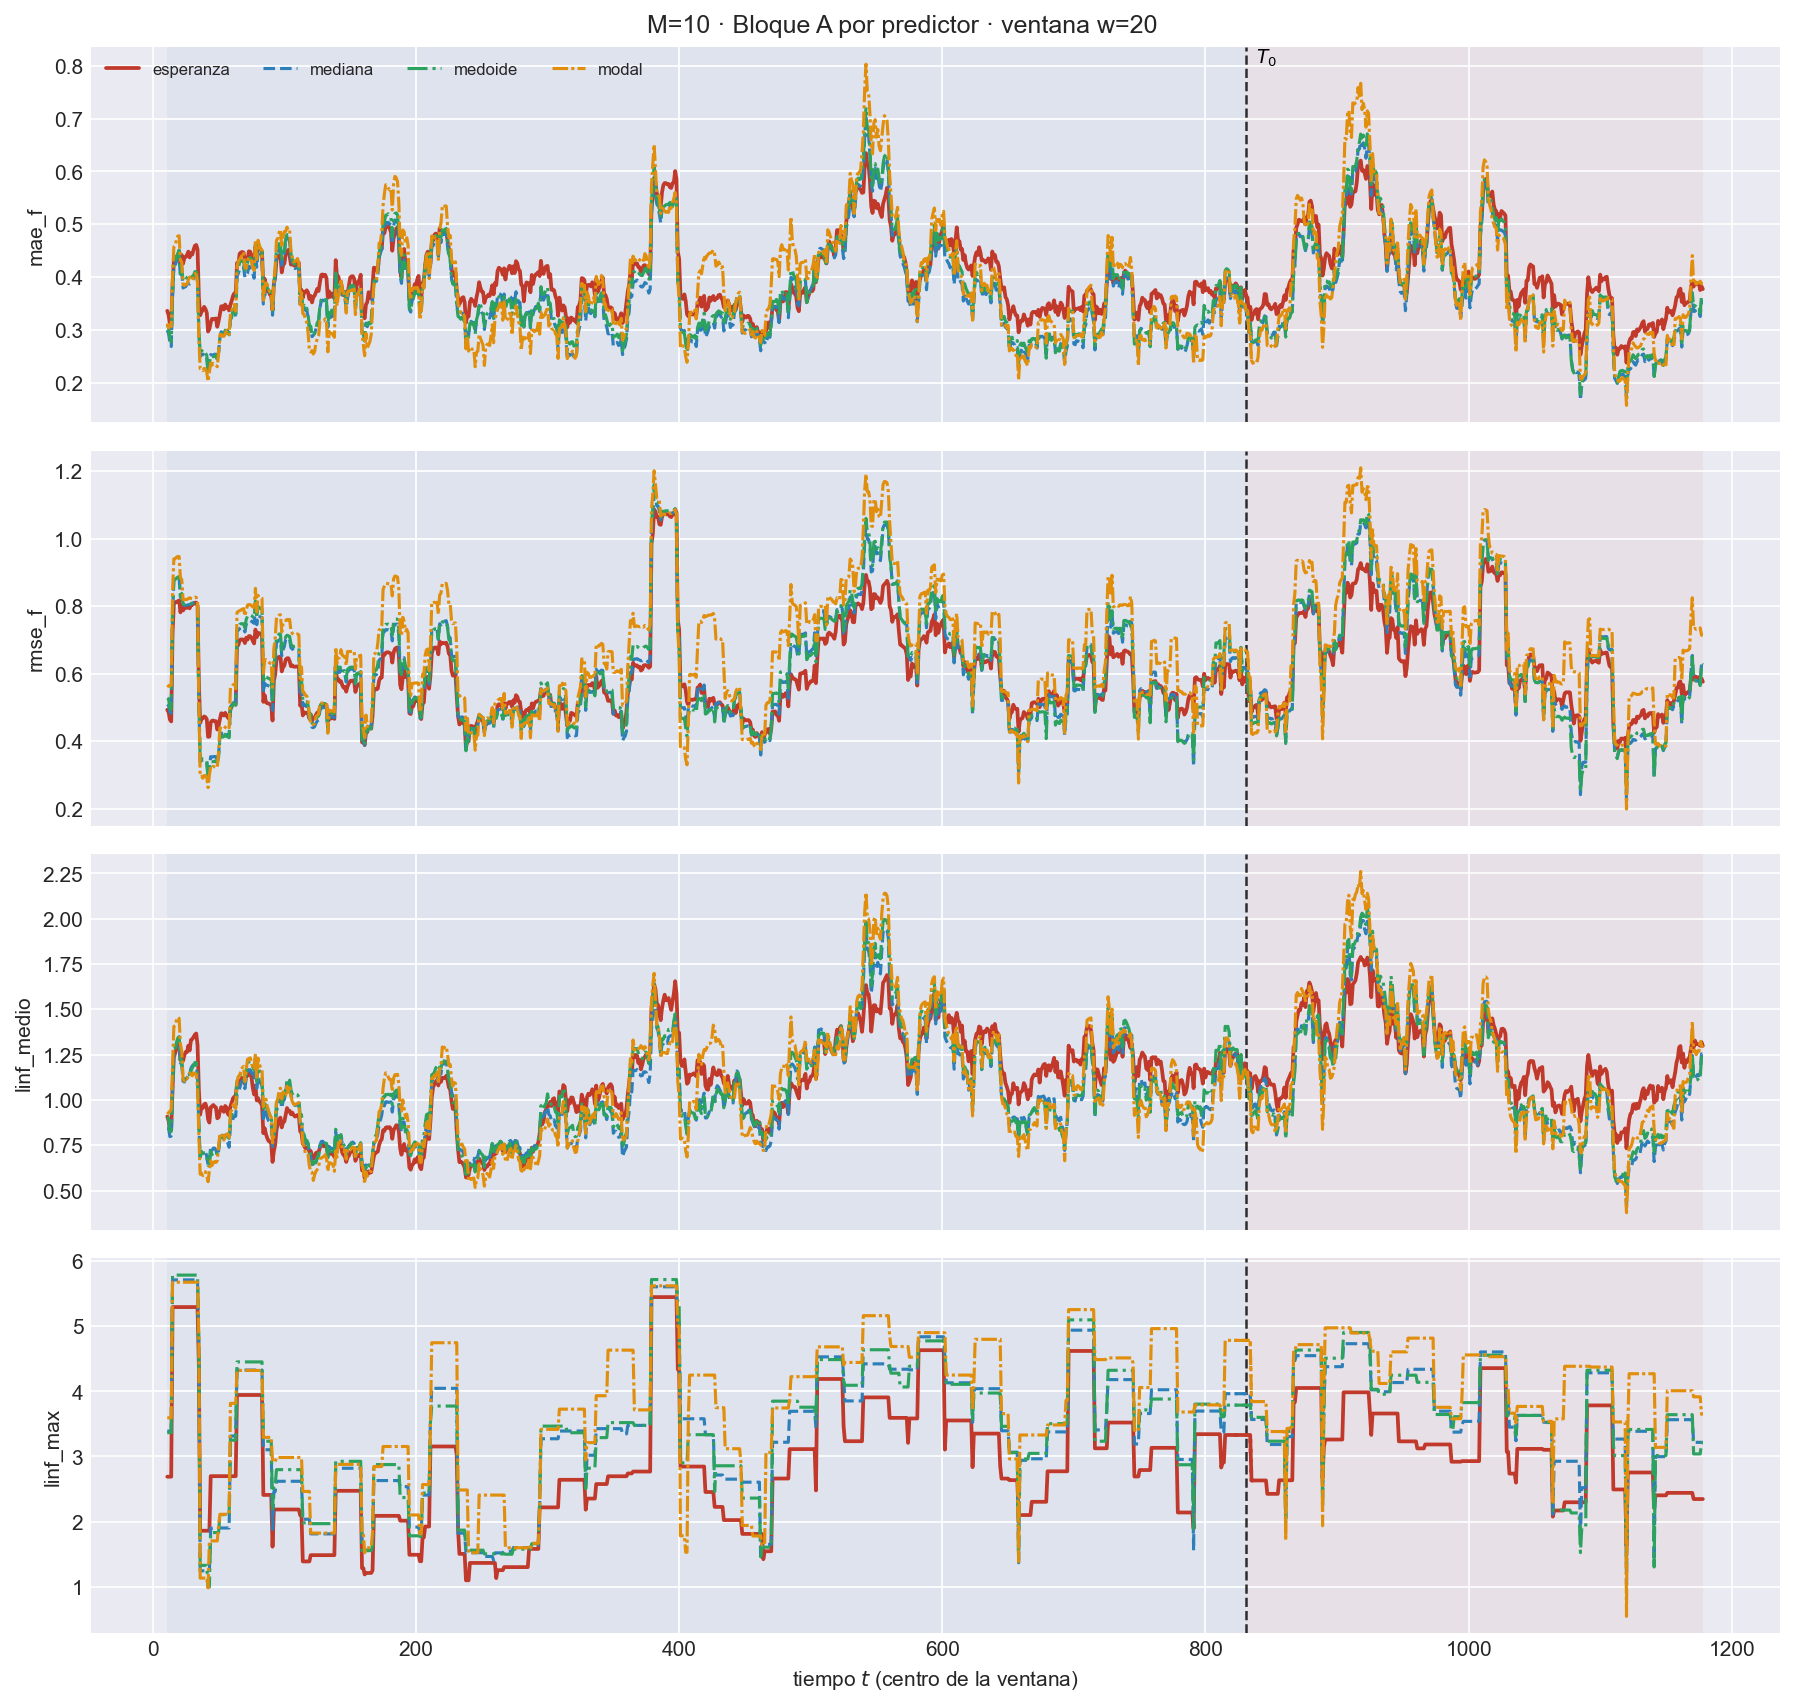
\includegraphics[width=\textwidth]{IMG/aneC_00/aneC_00_58_ventana_predictores_w20_101.png}
\caption{Métricas de error sobre la ventana móvil con $w = 20$, tráfico con rezago $\{1\}$ ($M = 10$).}
\label{fig:aneC_58_ventana_predictores_w20_101}
\end{figure}

\begin{figure}[H]
\centering
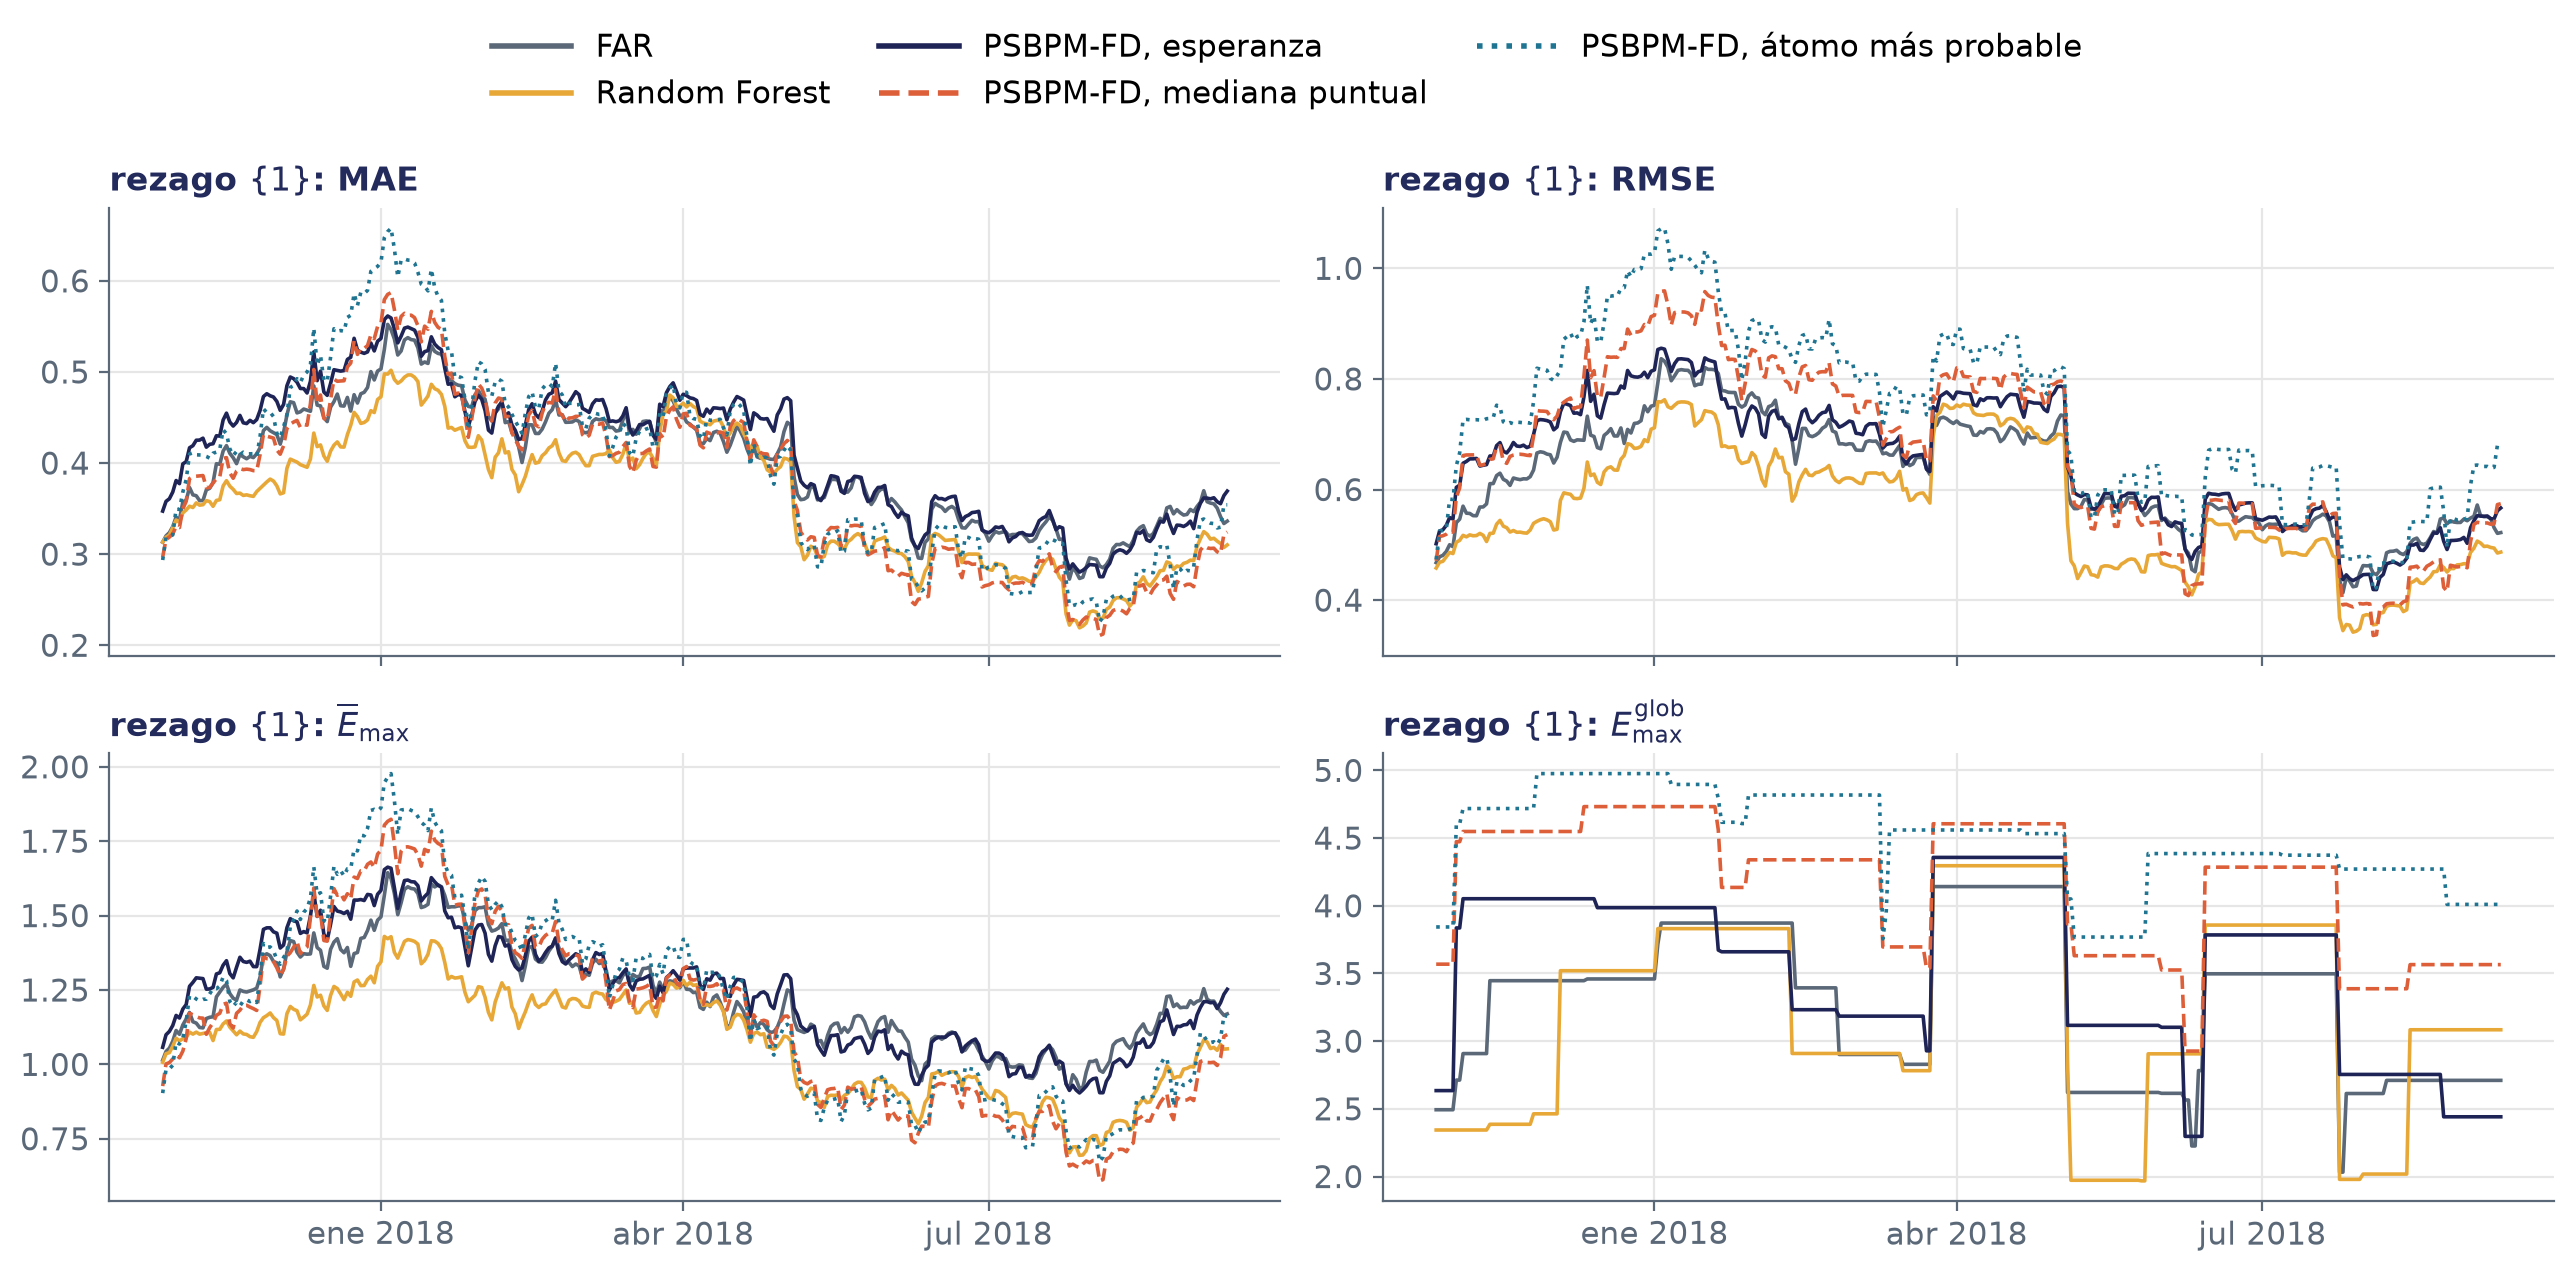
\includegraphics[width=\textwidth]{IMG/aneC_00/aneC_00_58_ventana_predictores_w40_101.png}
\caption{Métricas de error sobre la ventana móvil con $w = 40$, tráfico con rezago $\{1\}$ ($M = 10$).}
\label{fig:aneC_58_ventana_predictores_w40_101}
\end{figure}

\begin{figure}[H]
\centering
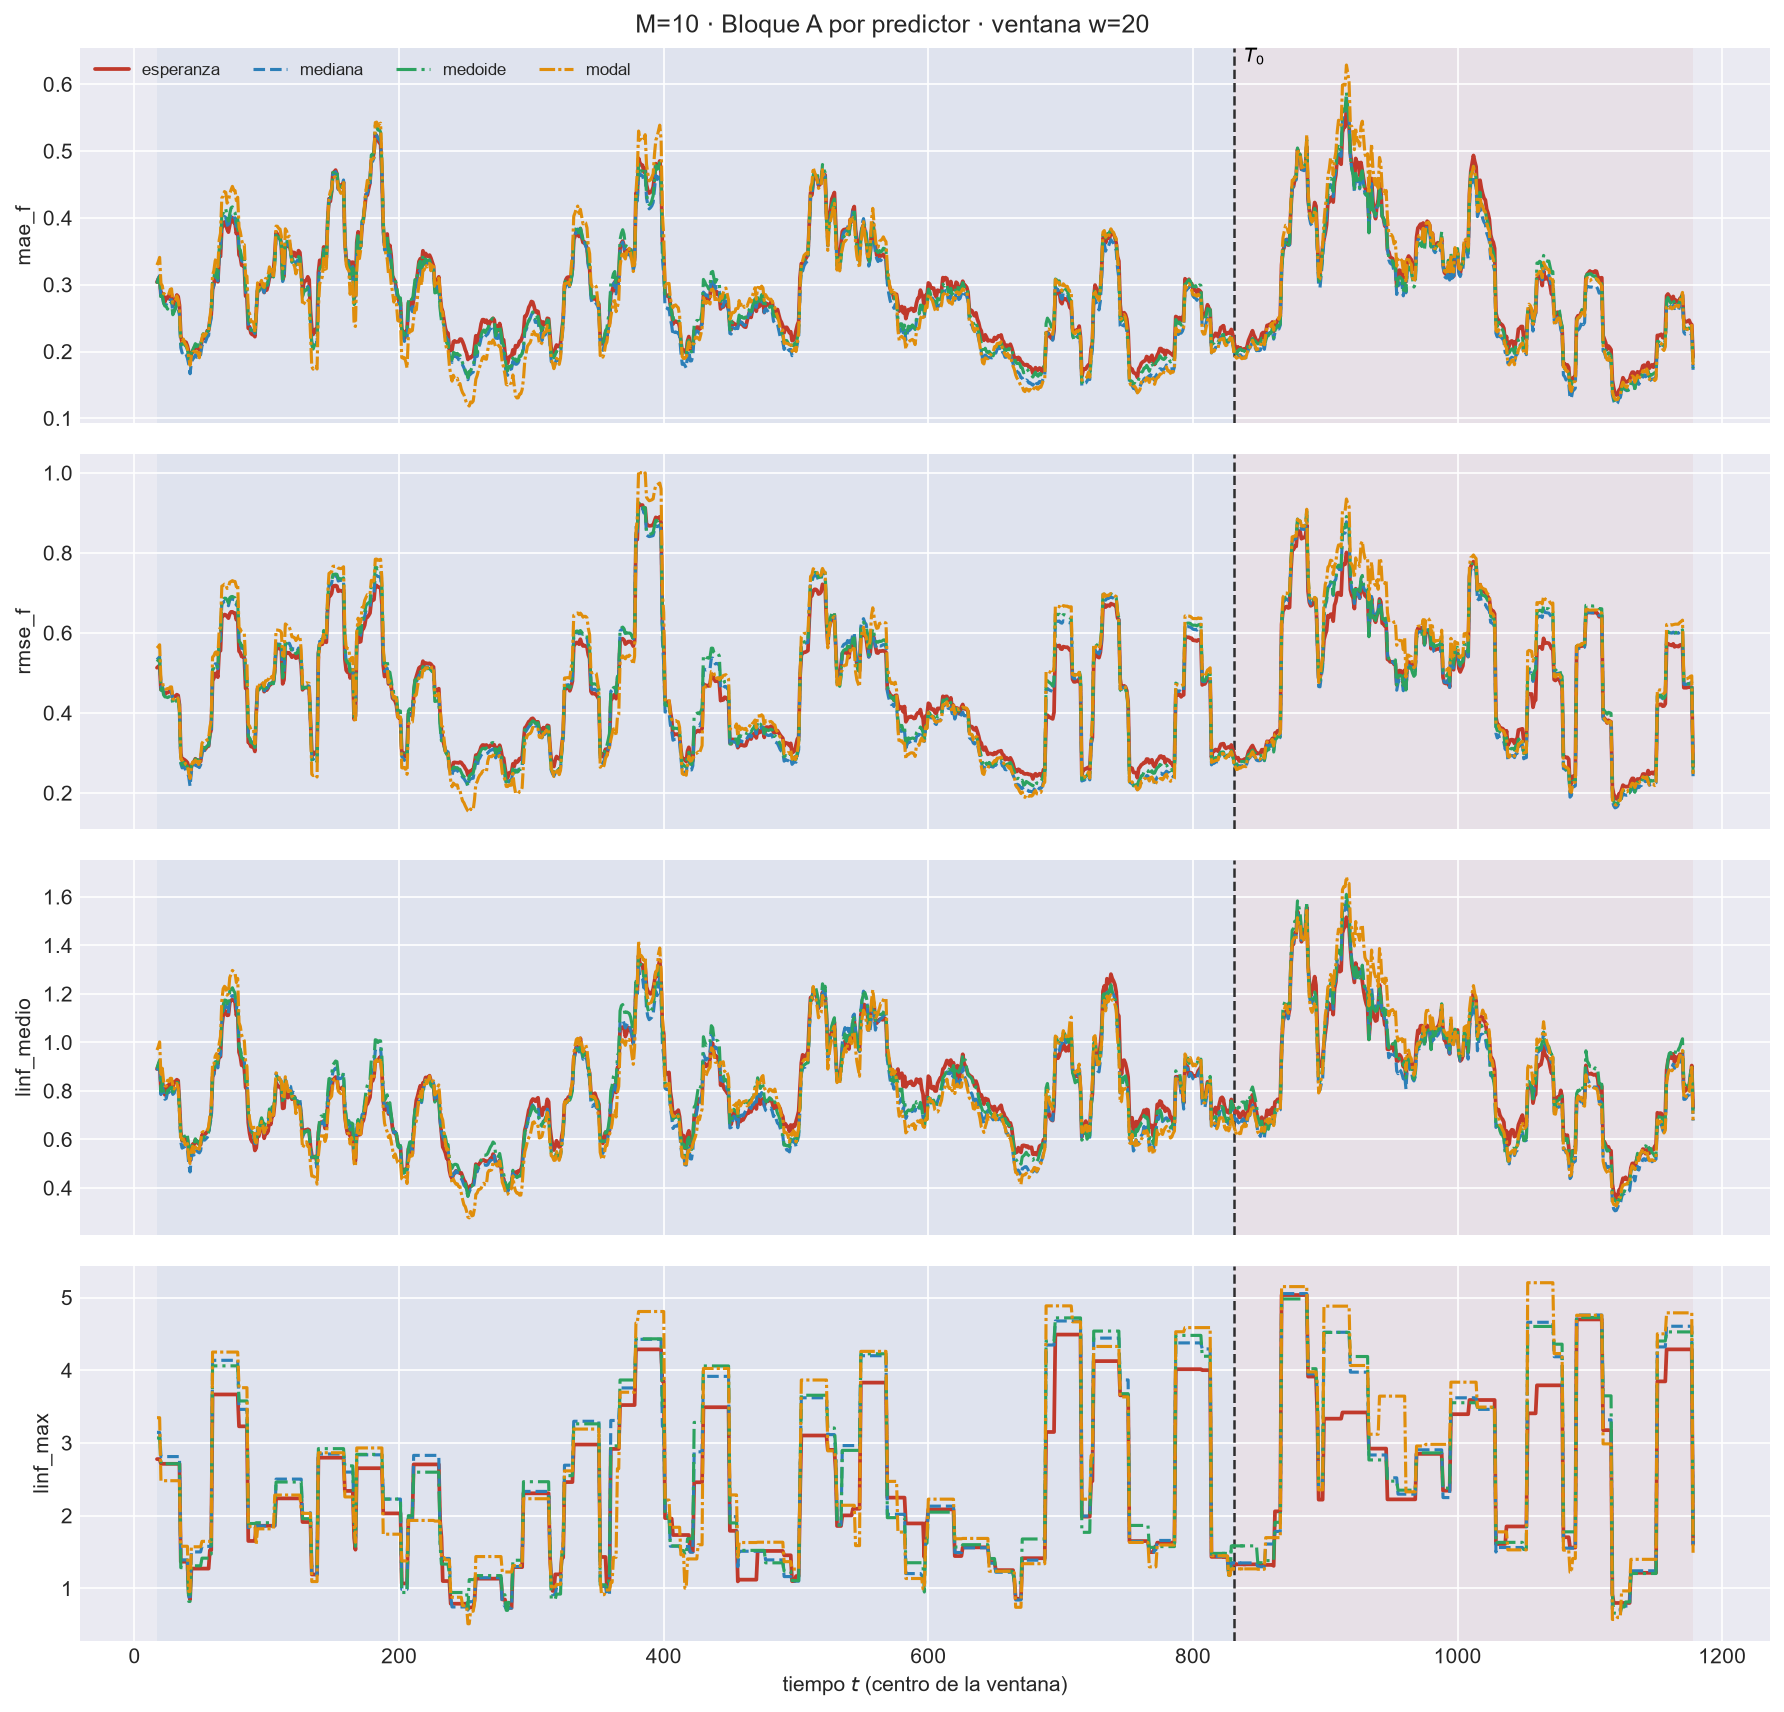
\includegraphics[width=\textwidth]{IMG/aneC_00/aneC_00_58_ventana_predictores_w20_102.png}
\caption{Métricas de error sobre la ventana móvil con $w = 20$, tráfico con rezagos $\{1,7\}$ ($M = 10$).}
\label{fig:aneC_58_ventana_predictores_w20_102}
\end{figure}

\begin{figure}[H]
\centering
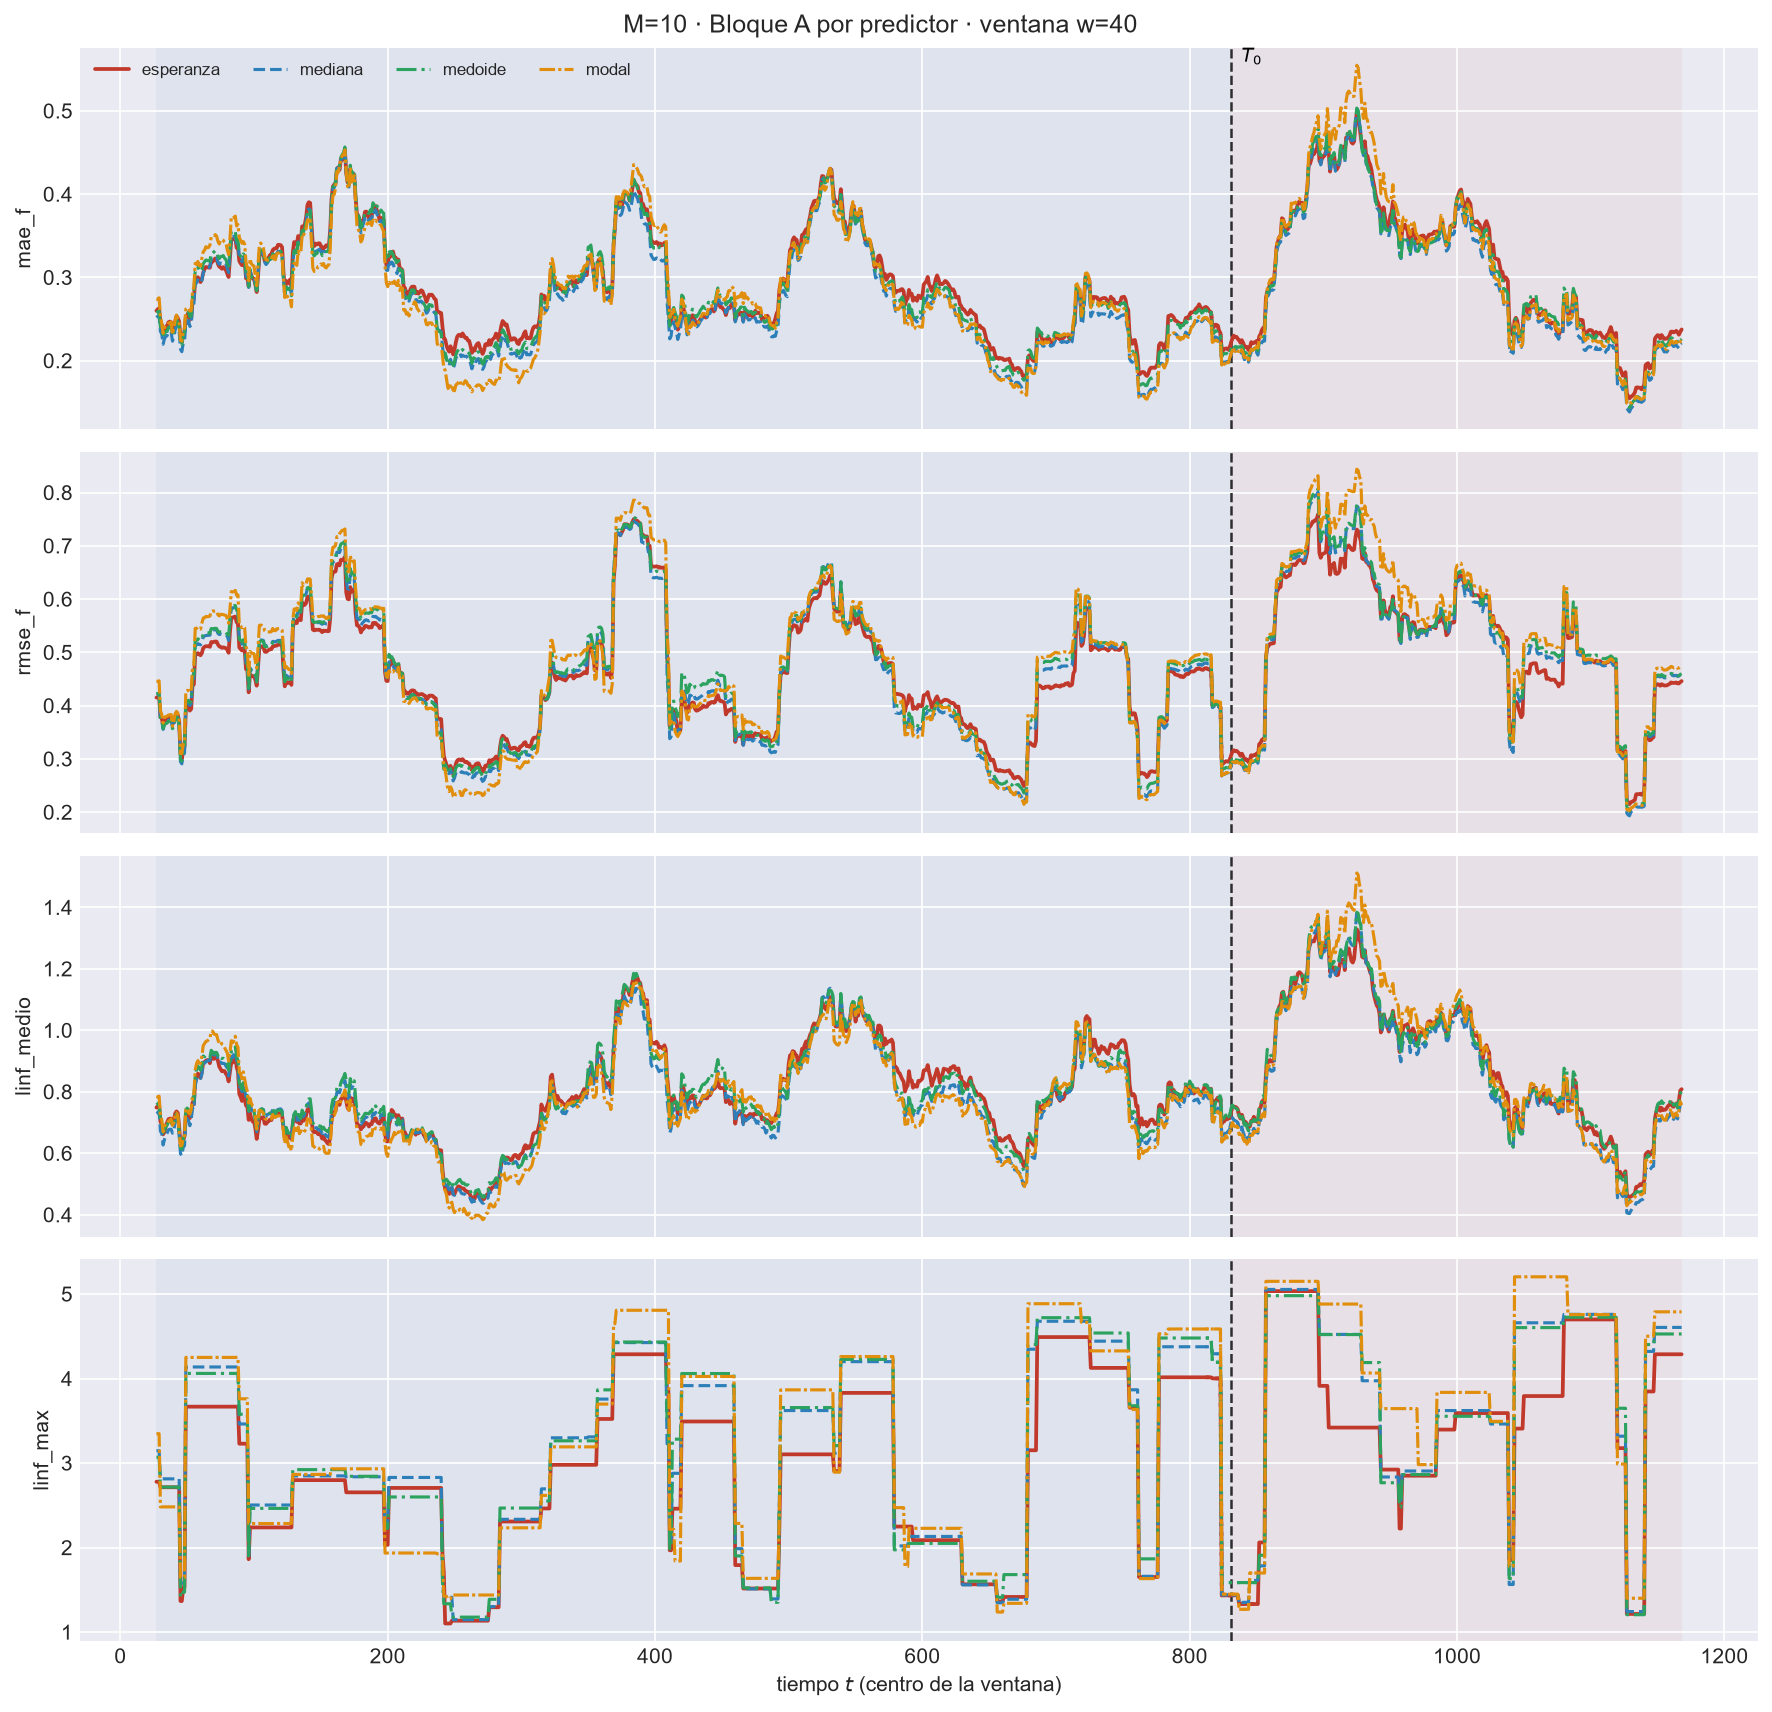
\includegraphics[width=\textwidth]{IMG/aneC_00/aneC_00_58_ventana_predictores_w40_102.png}
\caption{Métricas de error sobre la ventana móvil con $w = 40$, tráfico con rezagos $\{1,7\}$ ($M = 10$).}
\label{fig:aneC_58_ventana_predictores_w40_102}
\end{figure}

\begin{figure}[H]
\centering
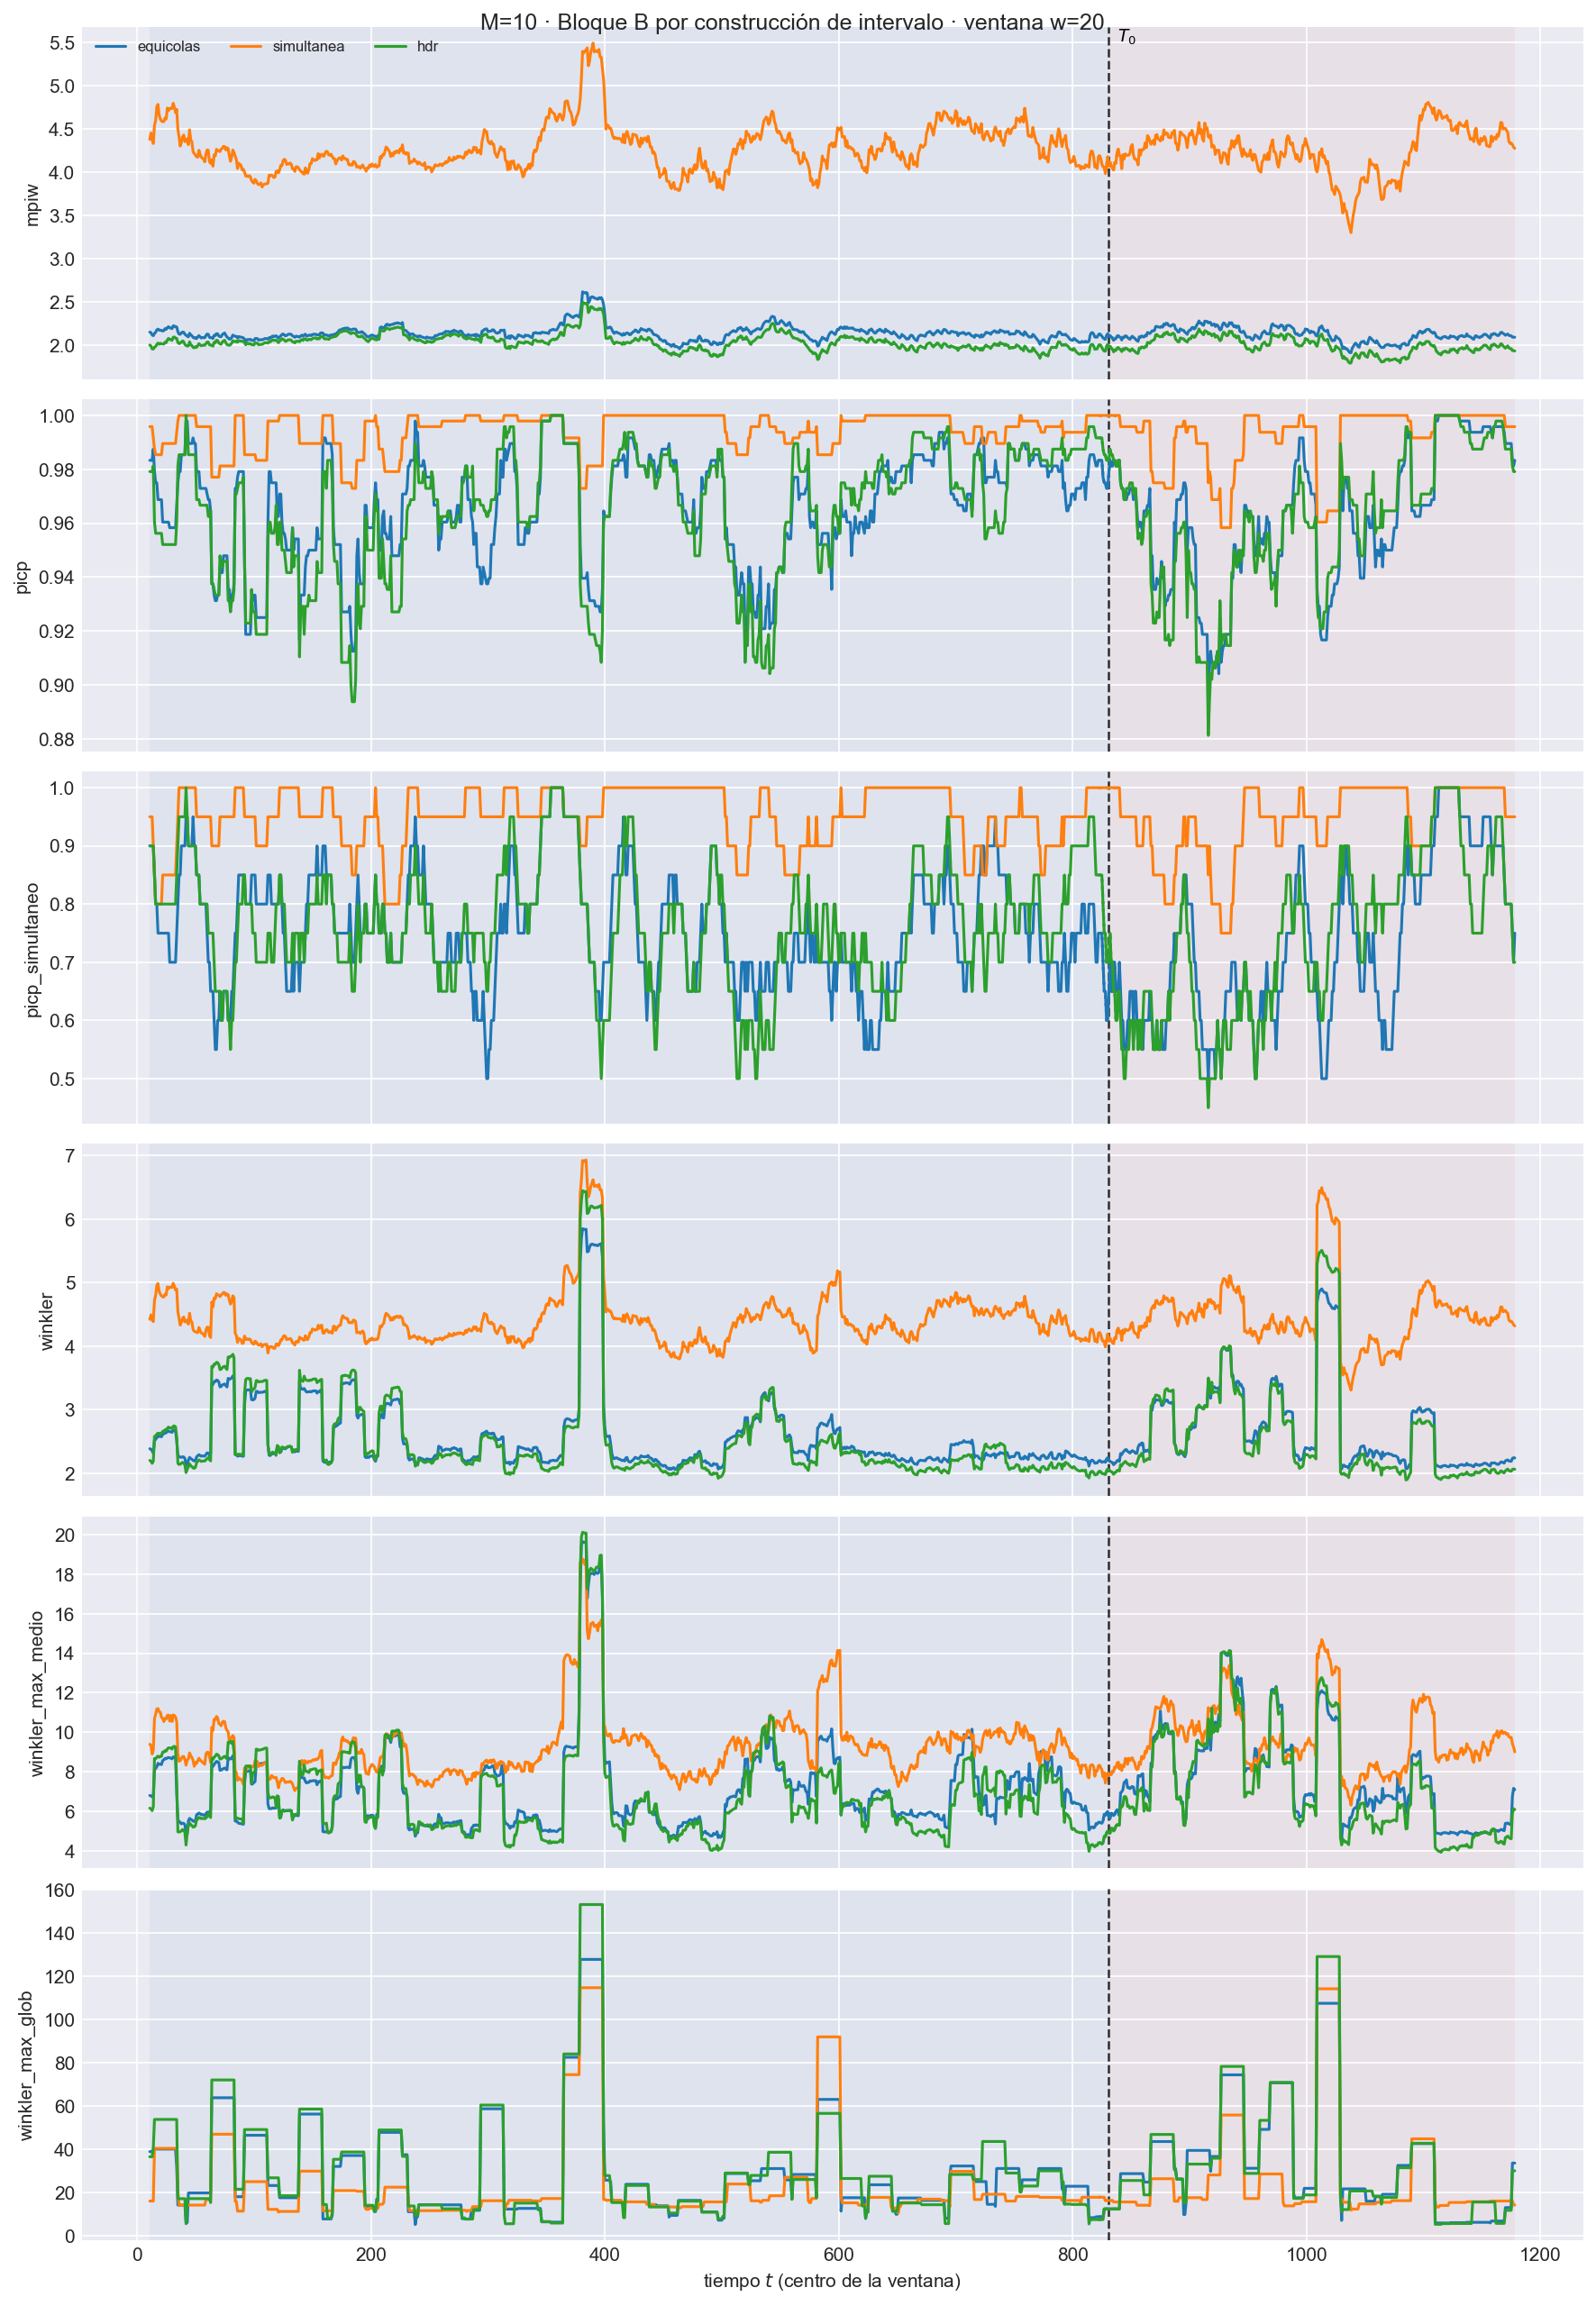
\includegraphics[width=\textwidth]{IMG/aneC_00/aneC_00_59_ventana_intervalos_w20_101.png}
\caption{Métricas de intervalo sobre la ventana móvil con $w = 20$, tráfico con rezago $\{1\}$ ($M = 10$).}
\label{fig:aneC_59_ventana_intervalos_w20_101}
\end{figure}

\begin{figure}[H]
\centering
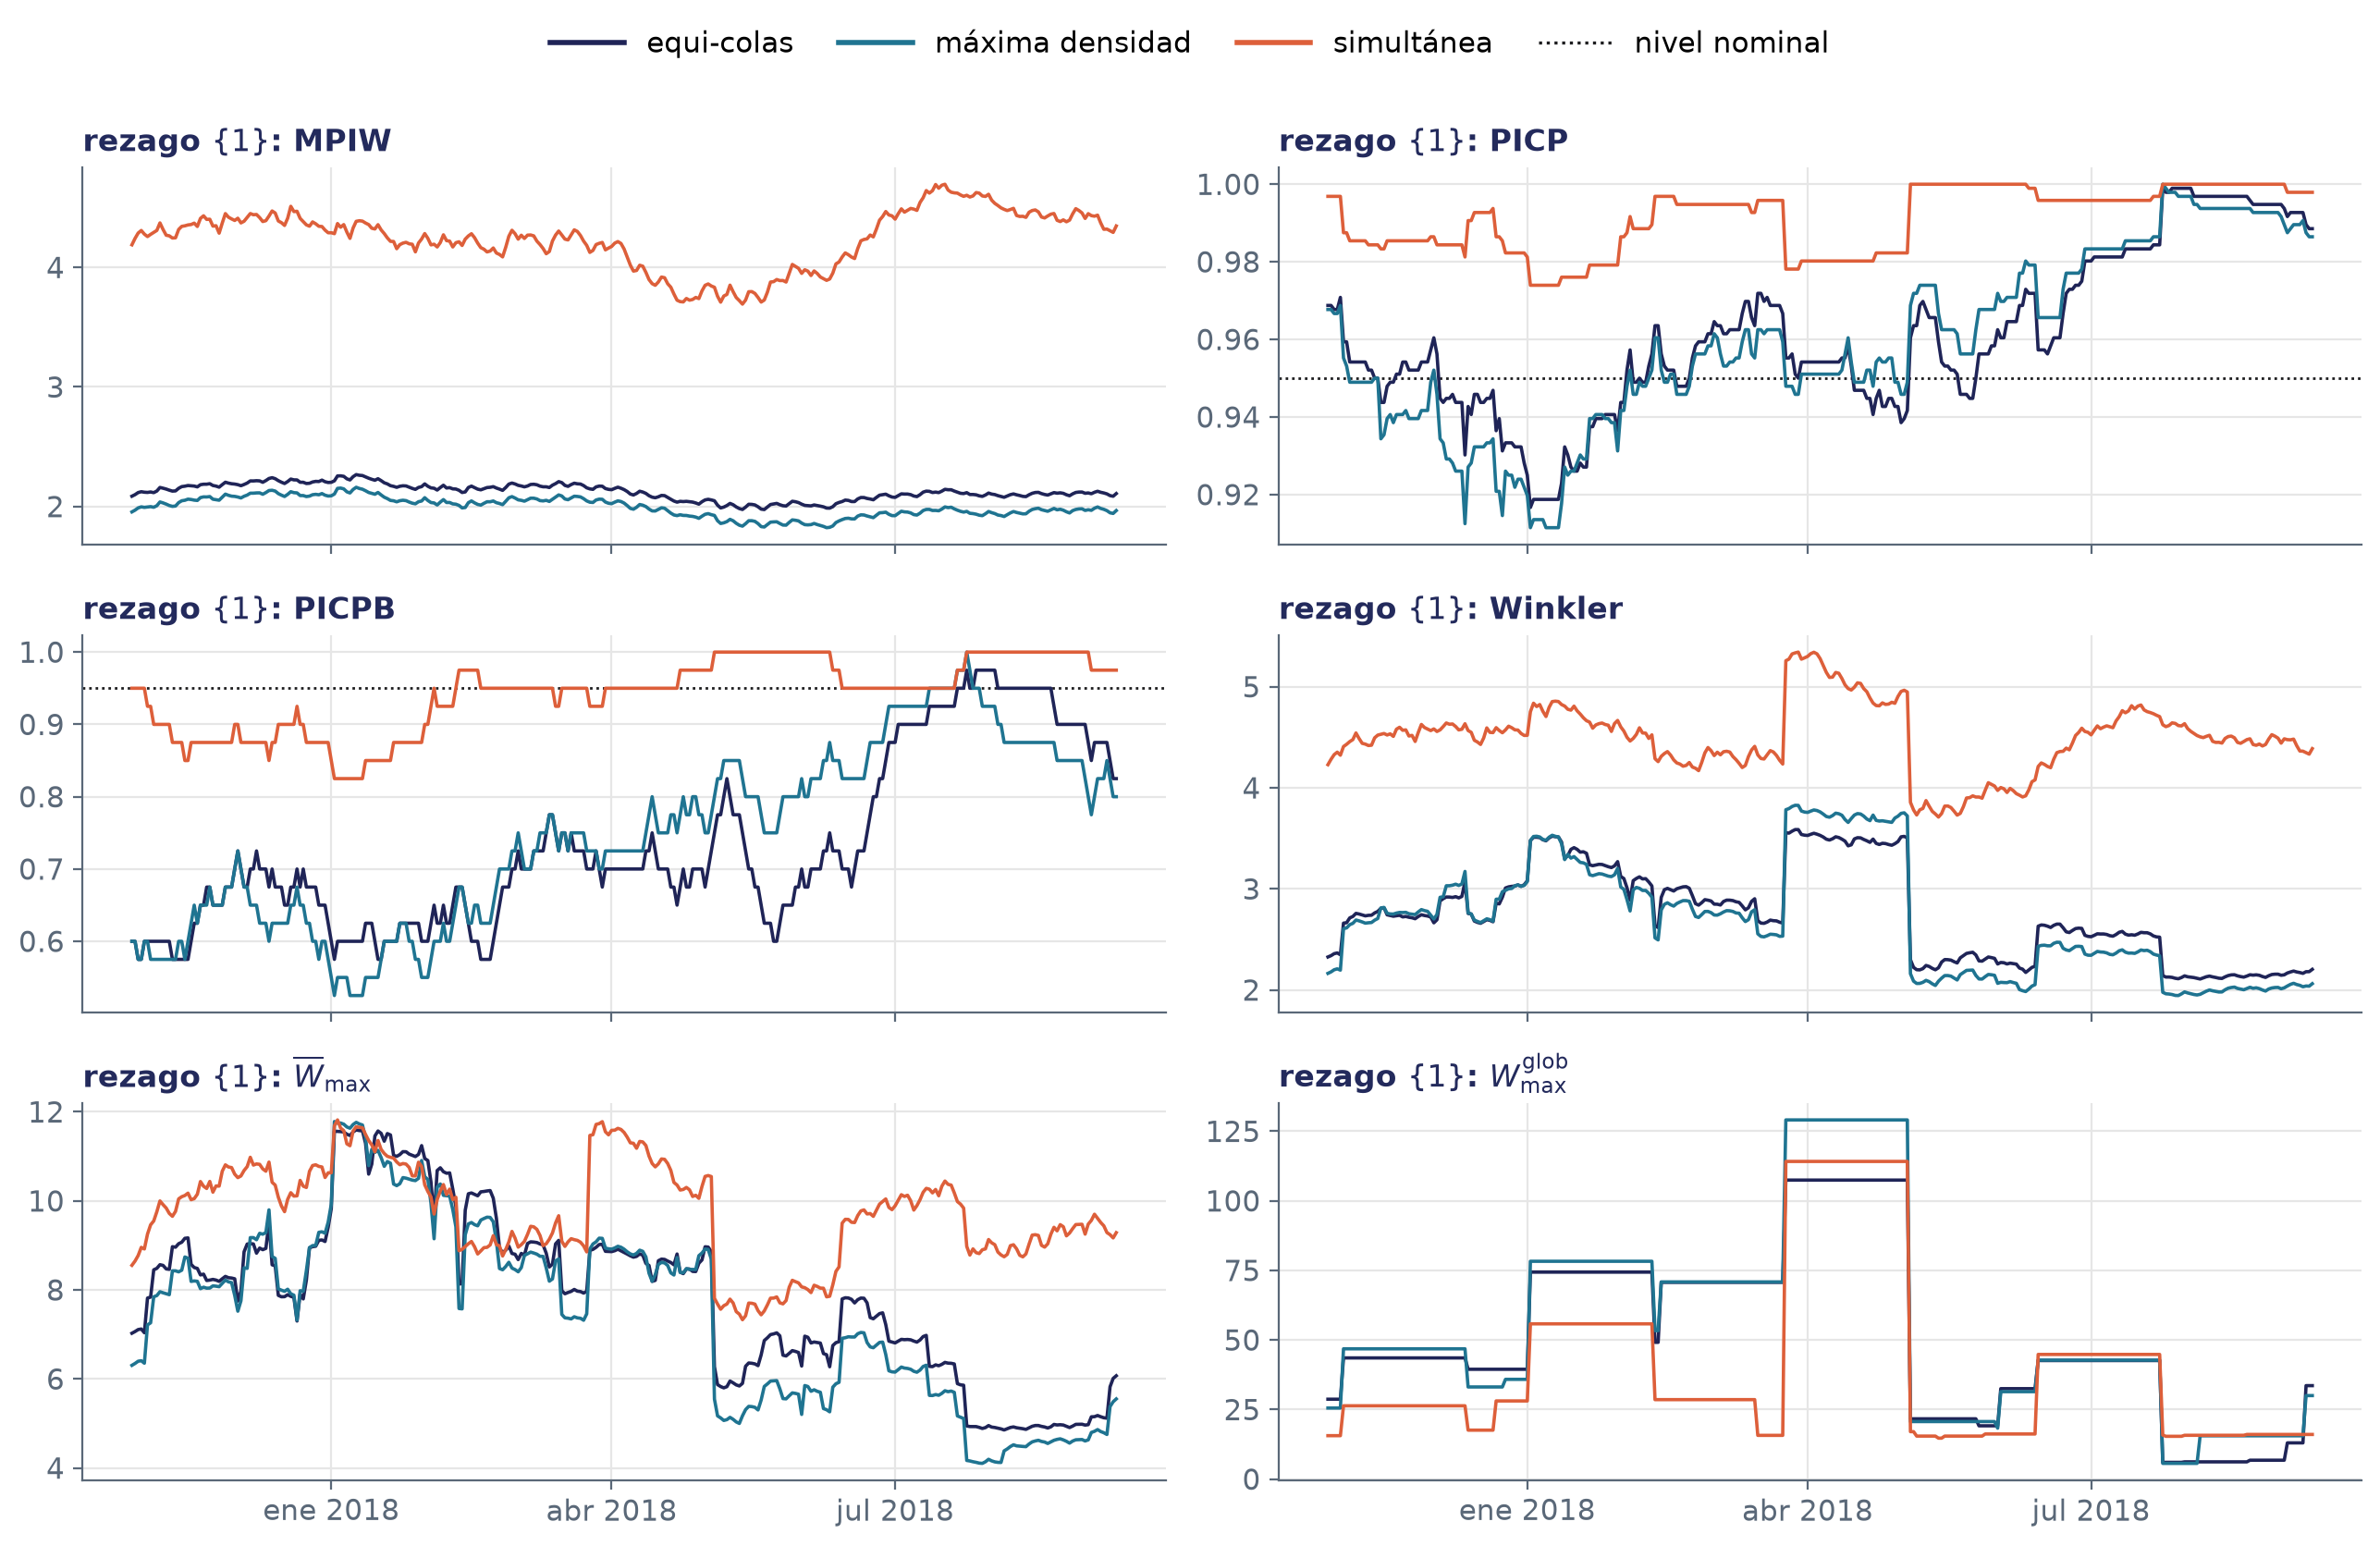
\includegraphics[width=\textwidth]{IMG/aneC_00/aneC_00_59_ventana_intervalos_w40_101.png}
\caption{Métricas de intervalo sobre la ventana móvil con $w = 40$, tráfico con rezago $\{1\}$ ($M = 10$).}
\label{fig:aneC_59_ventana_intervalos_w40_101}
\end{figure}

\begin{figure}[H]
\centering
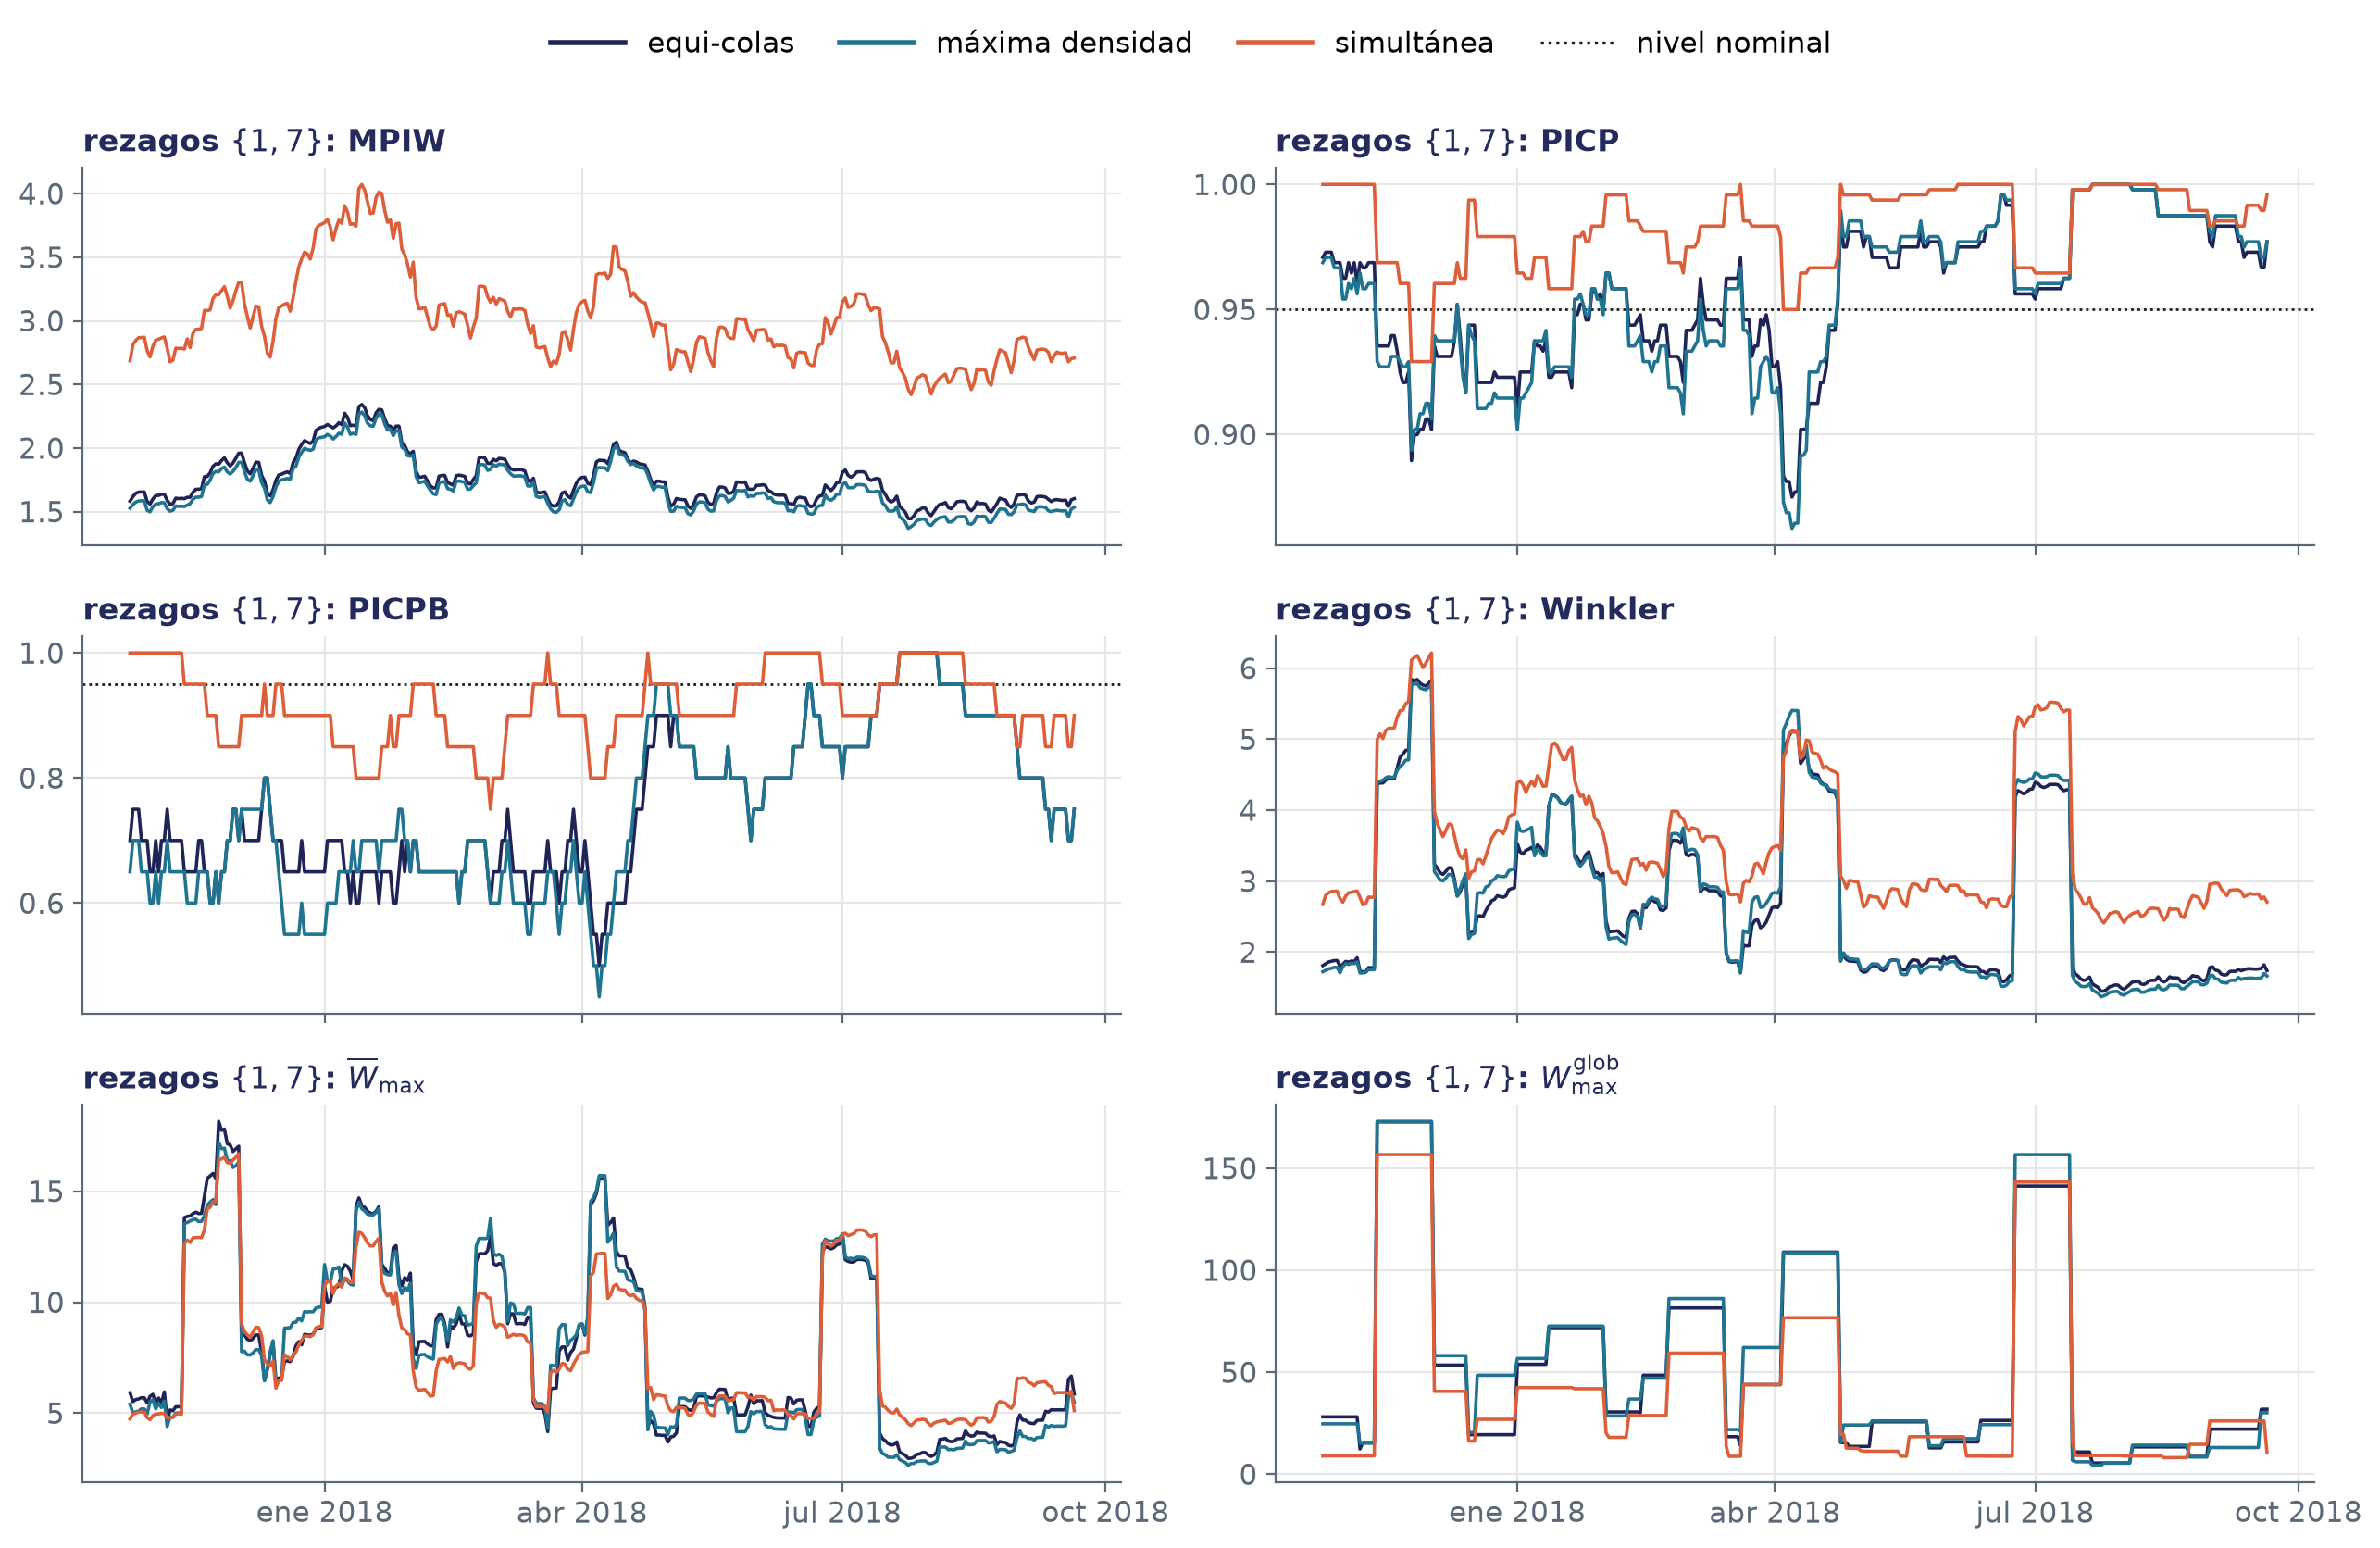
\includegraphics[width=\textwidth]{IMG/aneC_00/aneC_00_59_ventana_intervalos_w20_102.png}
\caption{Métricas de intervalo sobre la ventana móvil con $w = 20$, tráfico con rezagos $\{1,7\}$ ($M = 10$).}
\label{fig:aneC_59_ventana_intervalos_w20_102}
\end{figure}

\begin{figure}[H]
\centering
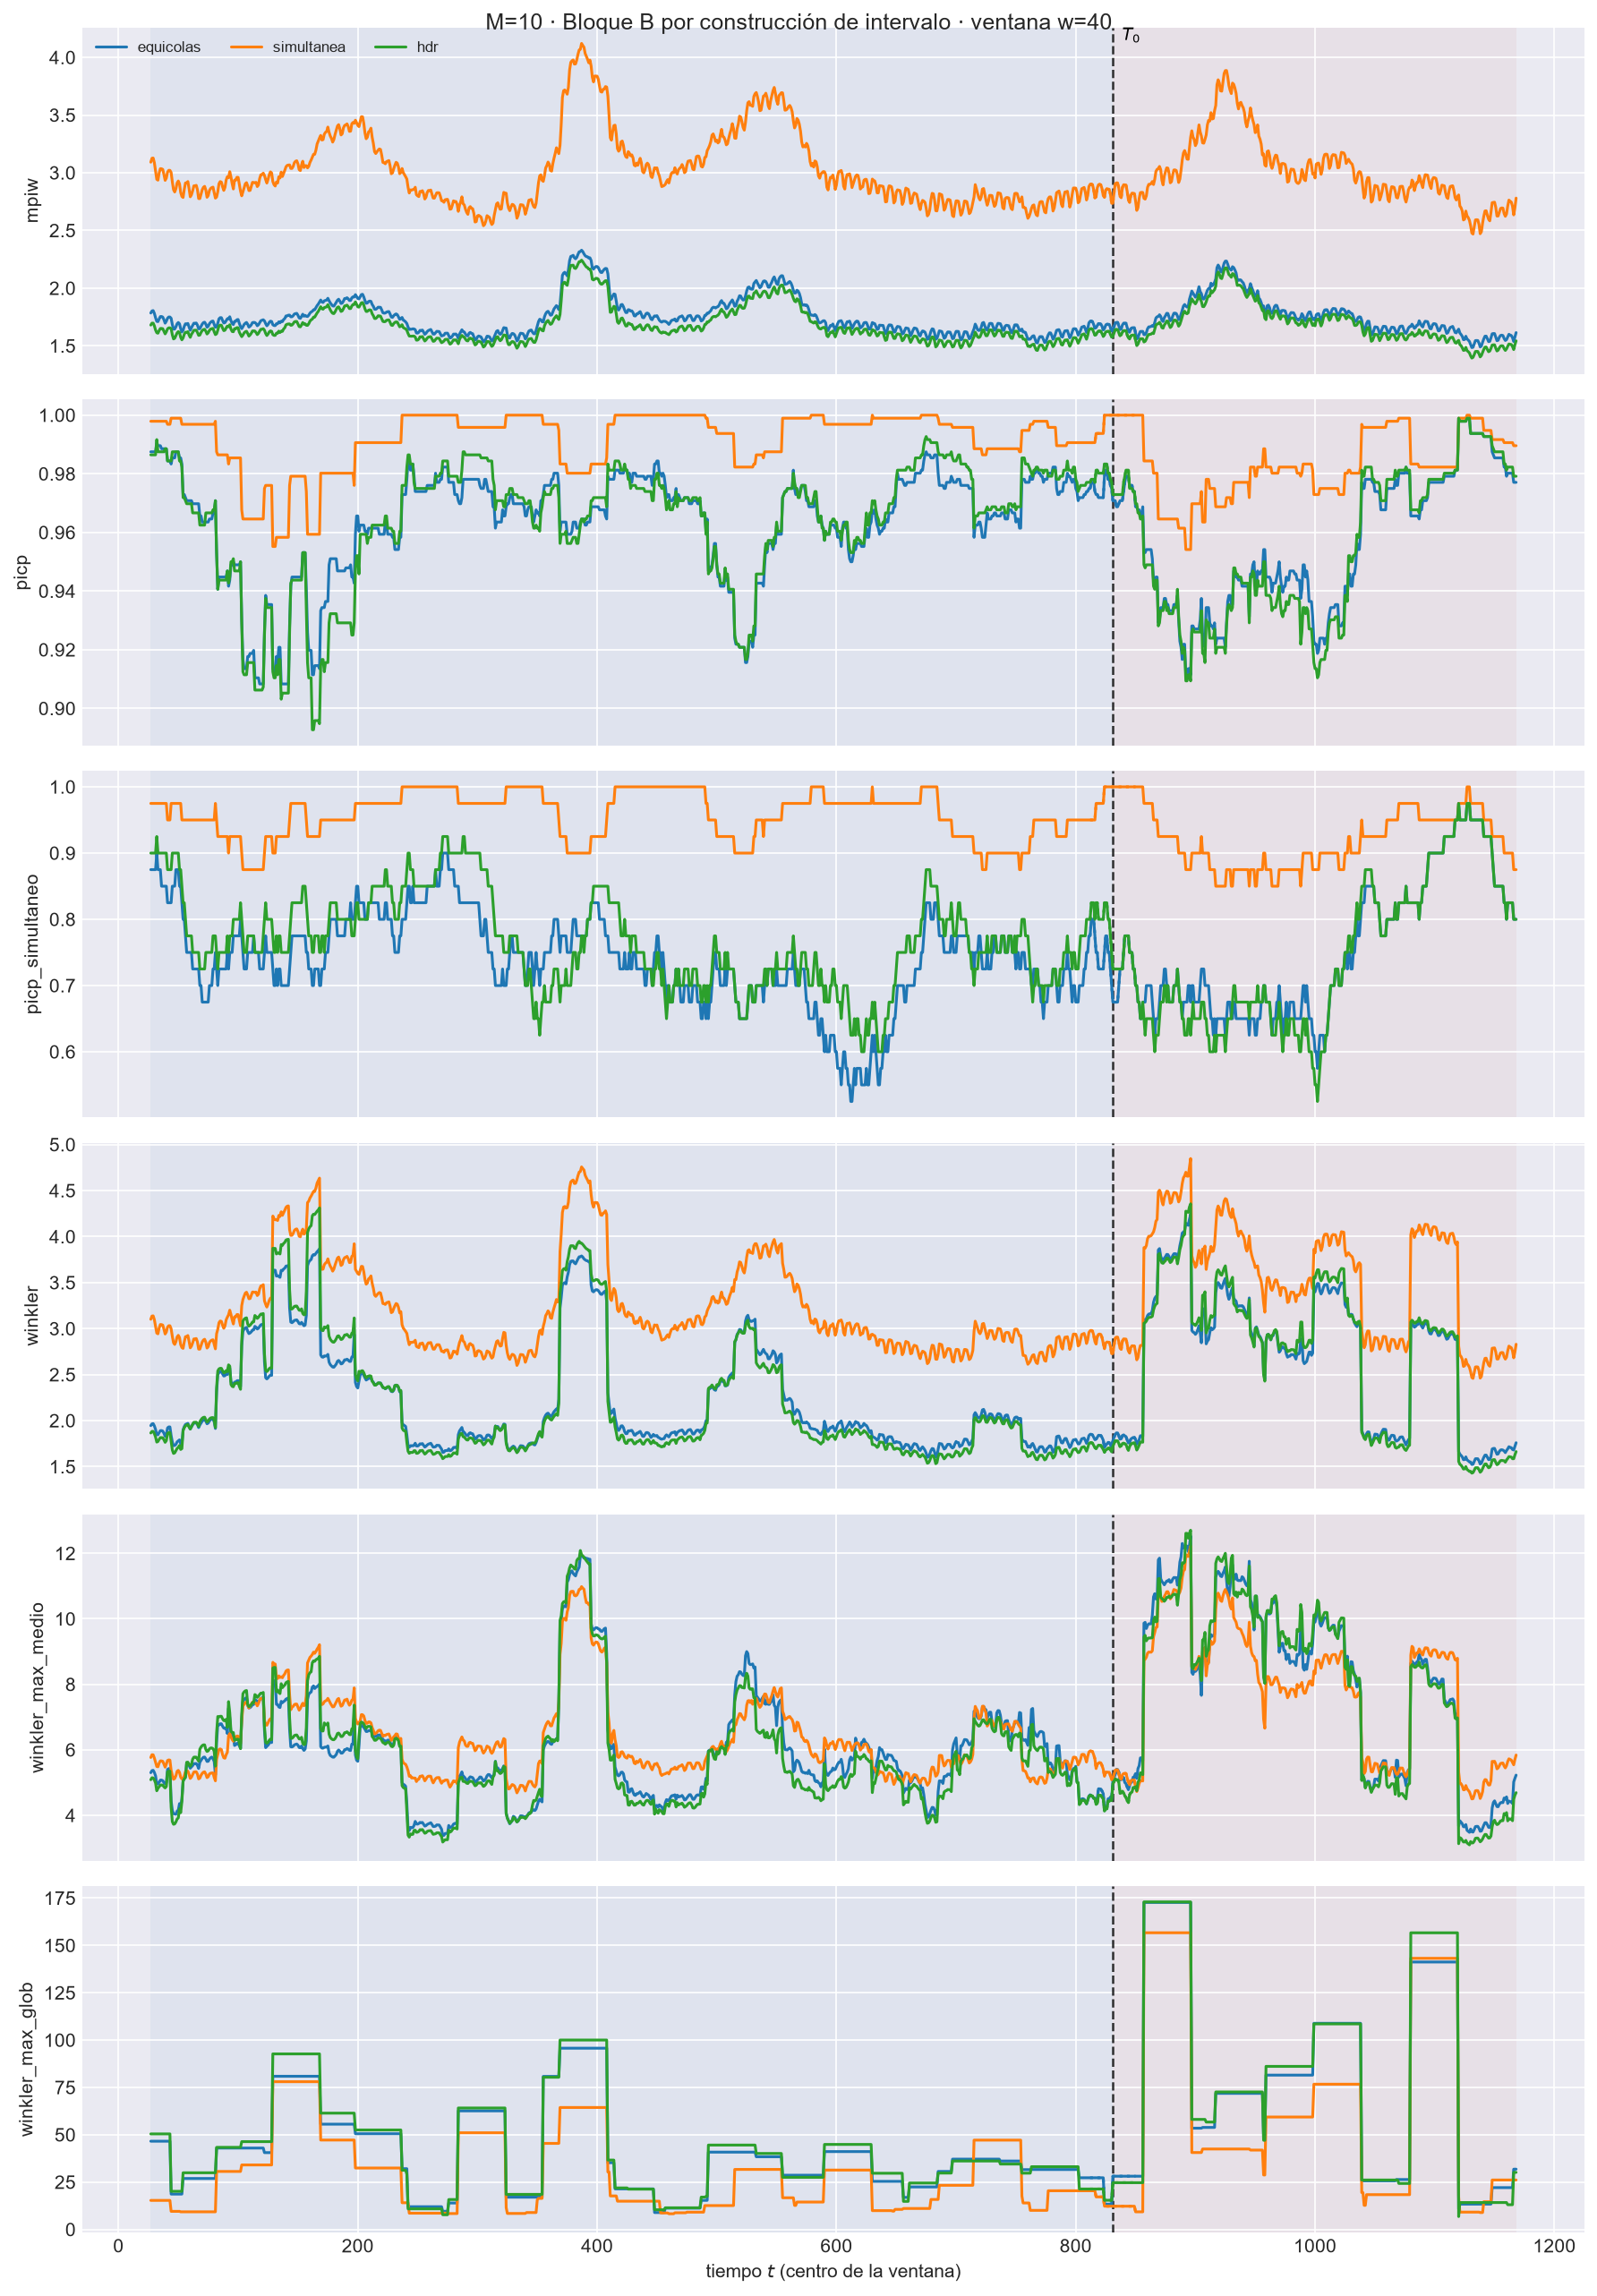
\includegraphics[width=\textwidth]{IMG/aneC_00/aneC_00_59_ventana_intervalos_w40_102.png}
\caption{Métricas de intervalo sobre la ventana móvil con $w = 40$, tráfico con rezagos $\{1,7\}$ ($M = 10$).}
\label{fig:aneC_59_ventana_intervalos_w40_102}
\end{figure}

\section{Predicciones curva a curva}
\label{aneC_00_05_curvas}
% 54 y 55: extractos del bloque de prueba y de la frontera; 56b: el peor origen por RMSE; 61b: predictores.

Extractos de predicciones del bloque de prueba, la ventana de peor RMSE y los tres predictores puntuales en cuatro orígenes de la ventana de detalle.

\begin{figure}[H]
\centering
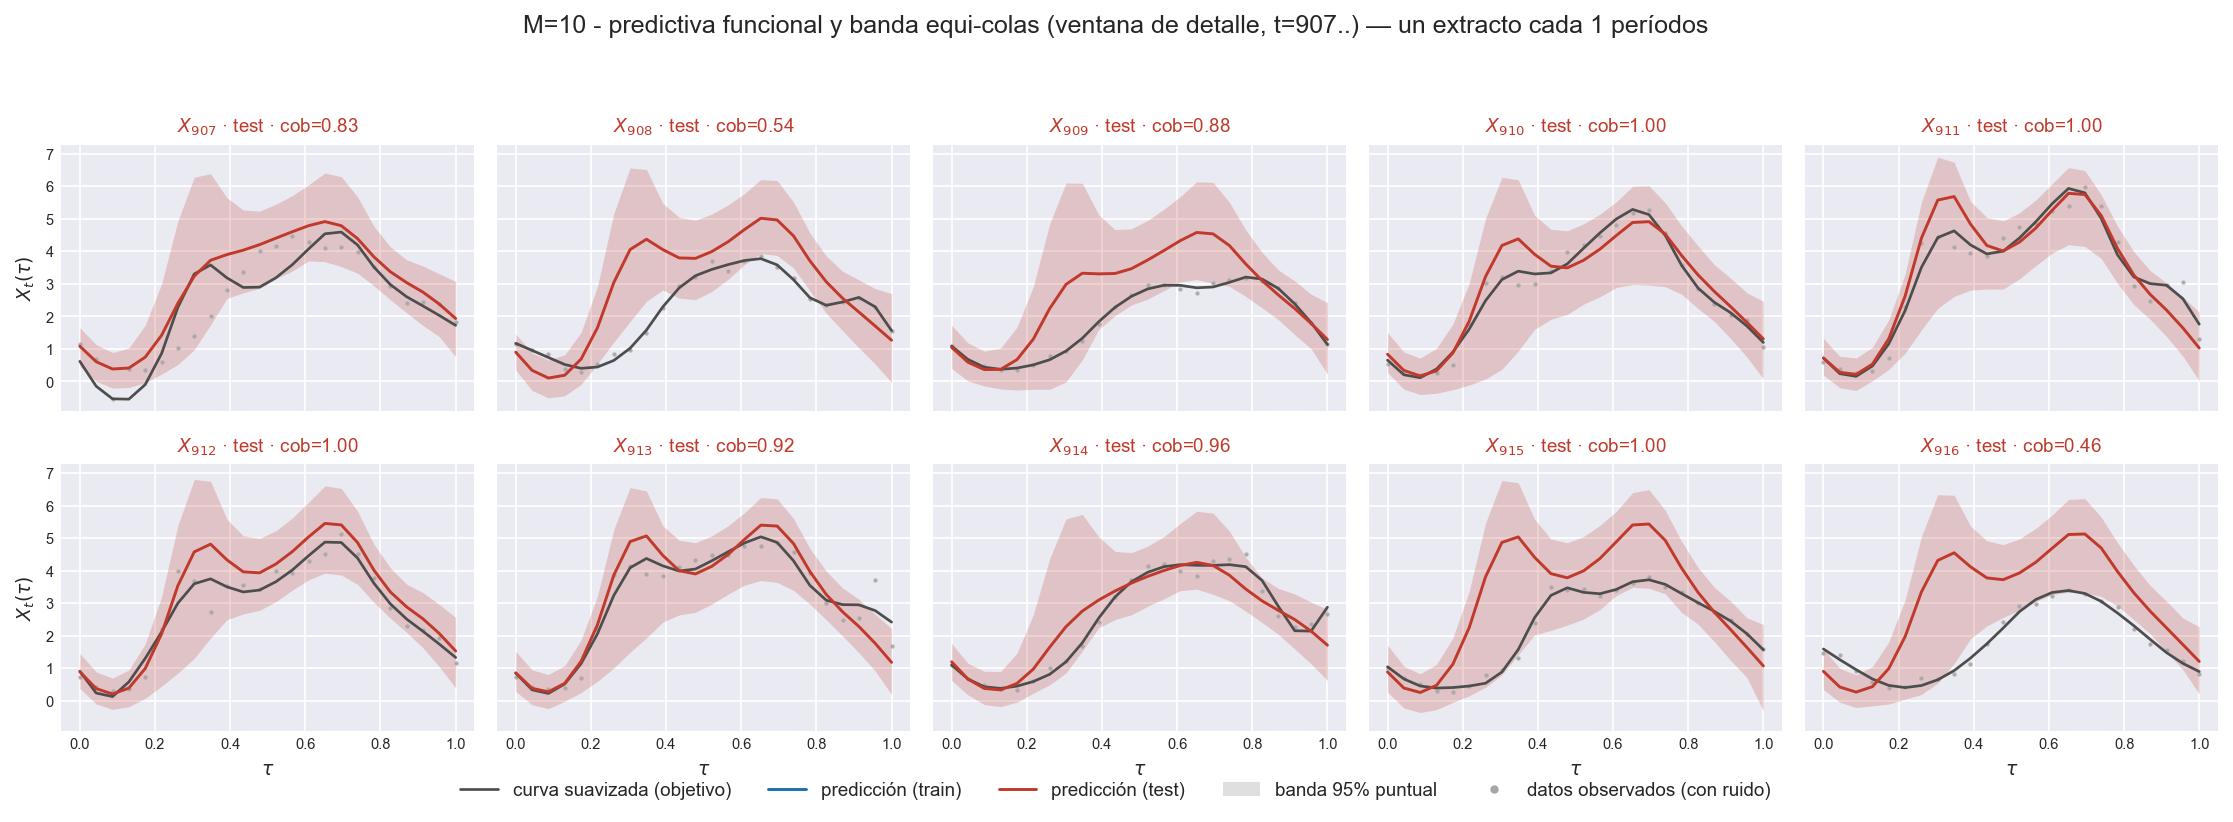
\includegraphics[width=\textwidth,height=0.8\textheight,keepaspectratio]{IMG/aneC_00/aneC_00_54_extractos_curvas_test_101.png}
\caption{Extractos de predicciones del bloque de prueba, tráfico con rezago $\{1\}$ ($M = 10$).}
\label{fig:aneC_54_extractos_curvas_test_101}
\end{figure}

\begin{figure}[H]
\centering
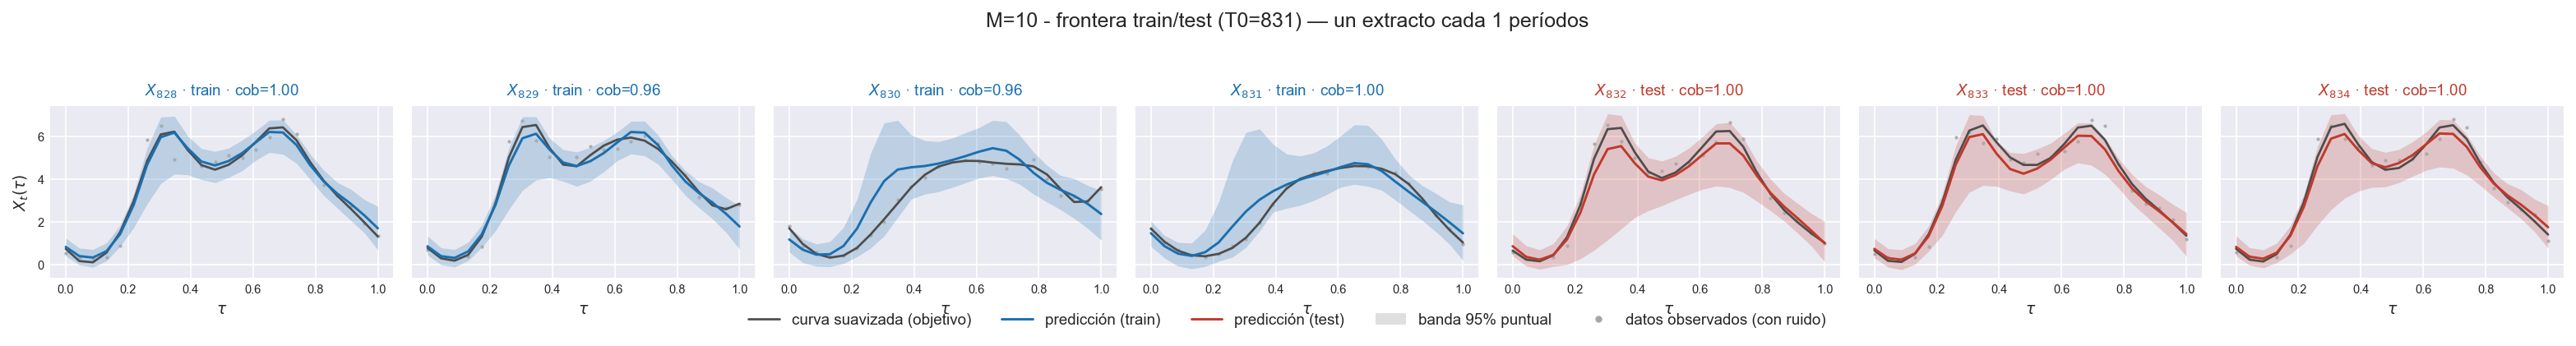
\includegraphics[width=\textwidth,height=0.8\textheight,keepaspectratio]{IMG/aneC_00/aneC_00_55_extractos_frontera_101.png}
\caption{Predicciones en la frontera entre los bloques de entrenamiento y de prueba, tráfico con rezago $\{1\}$ ($M = 10$).}
\label{fig:aneC_55_extractos_frontera_101}
\end{figure}

\begin{figure}[H]
\centering
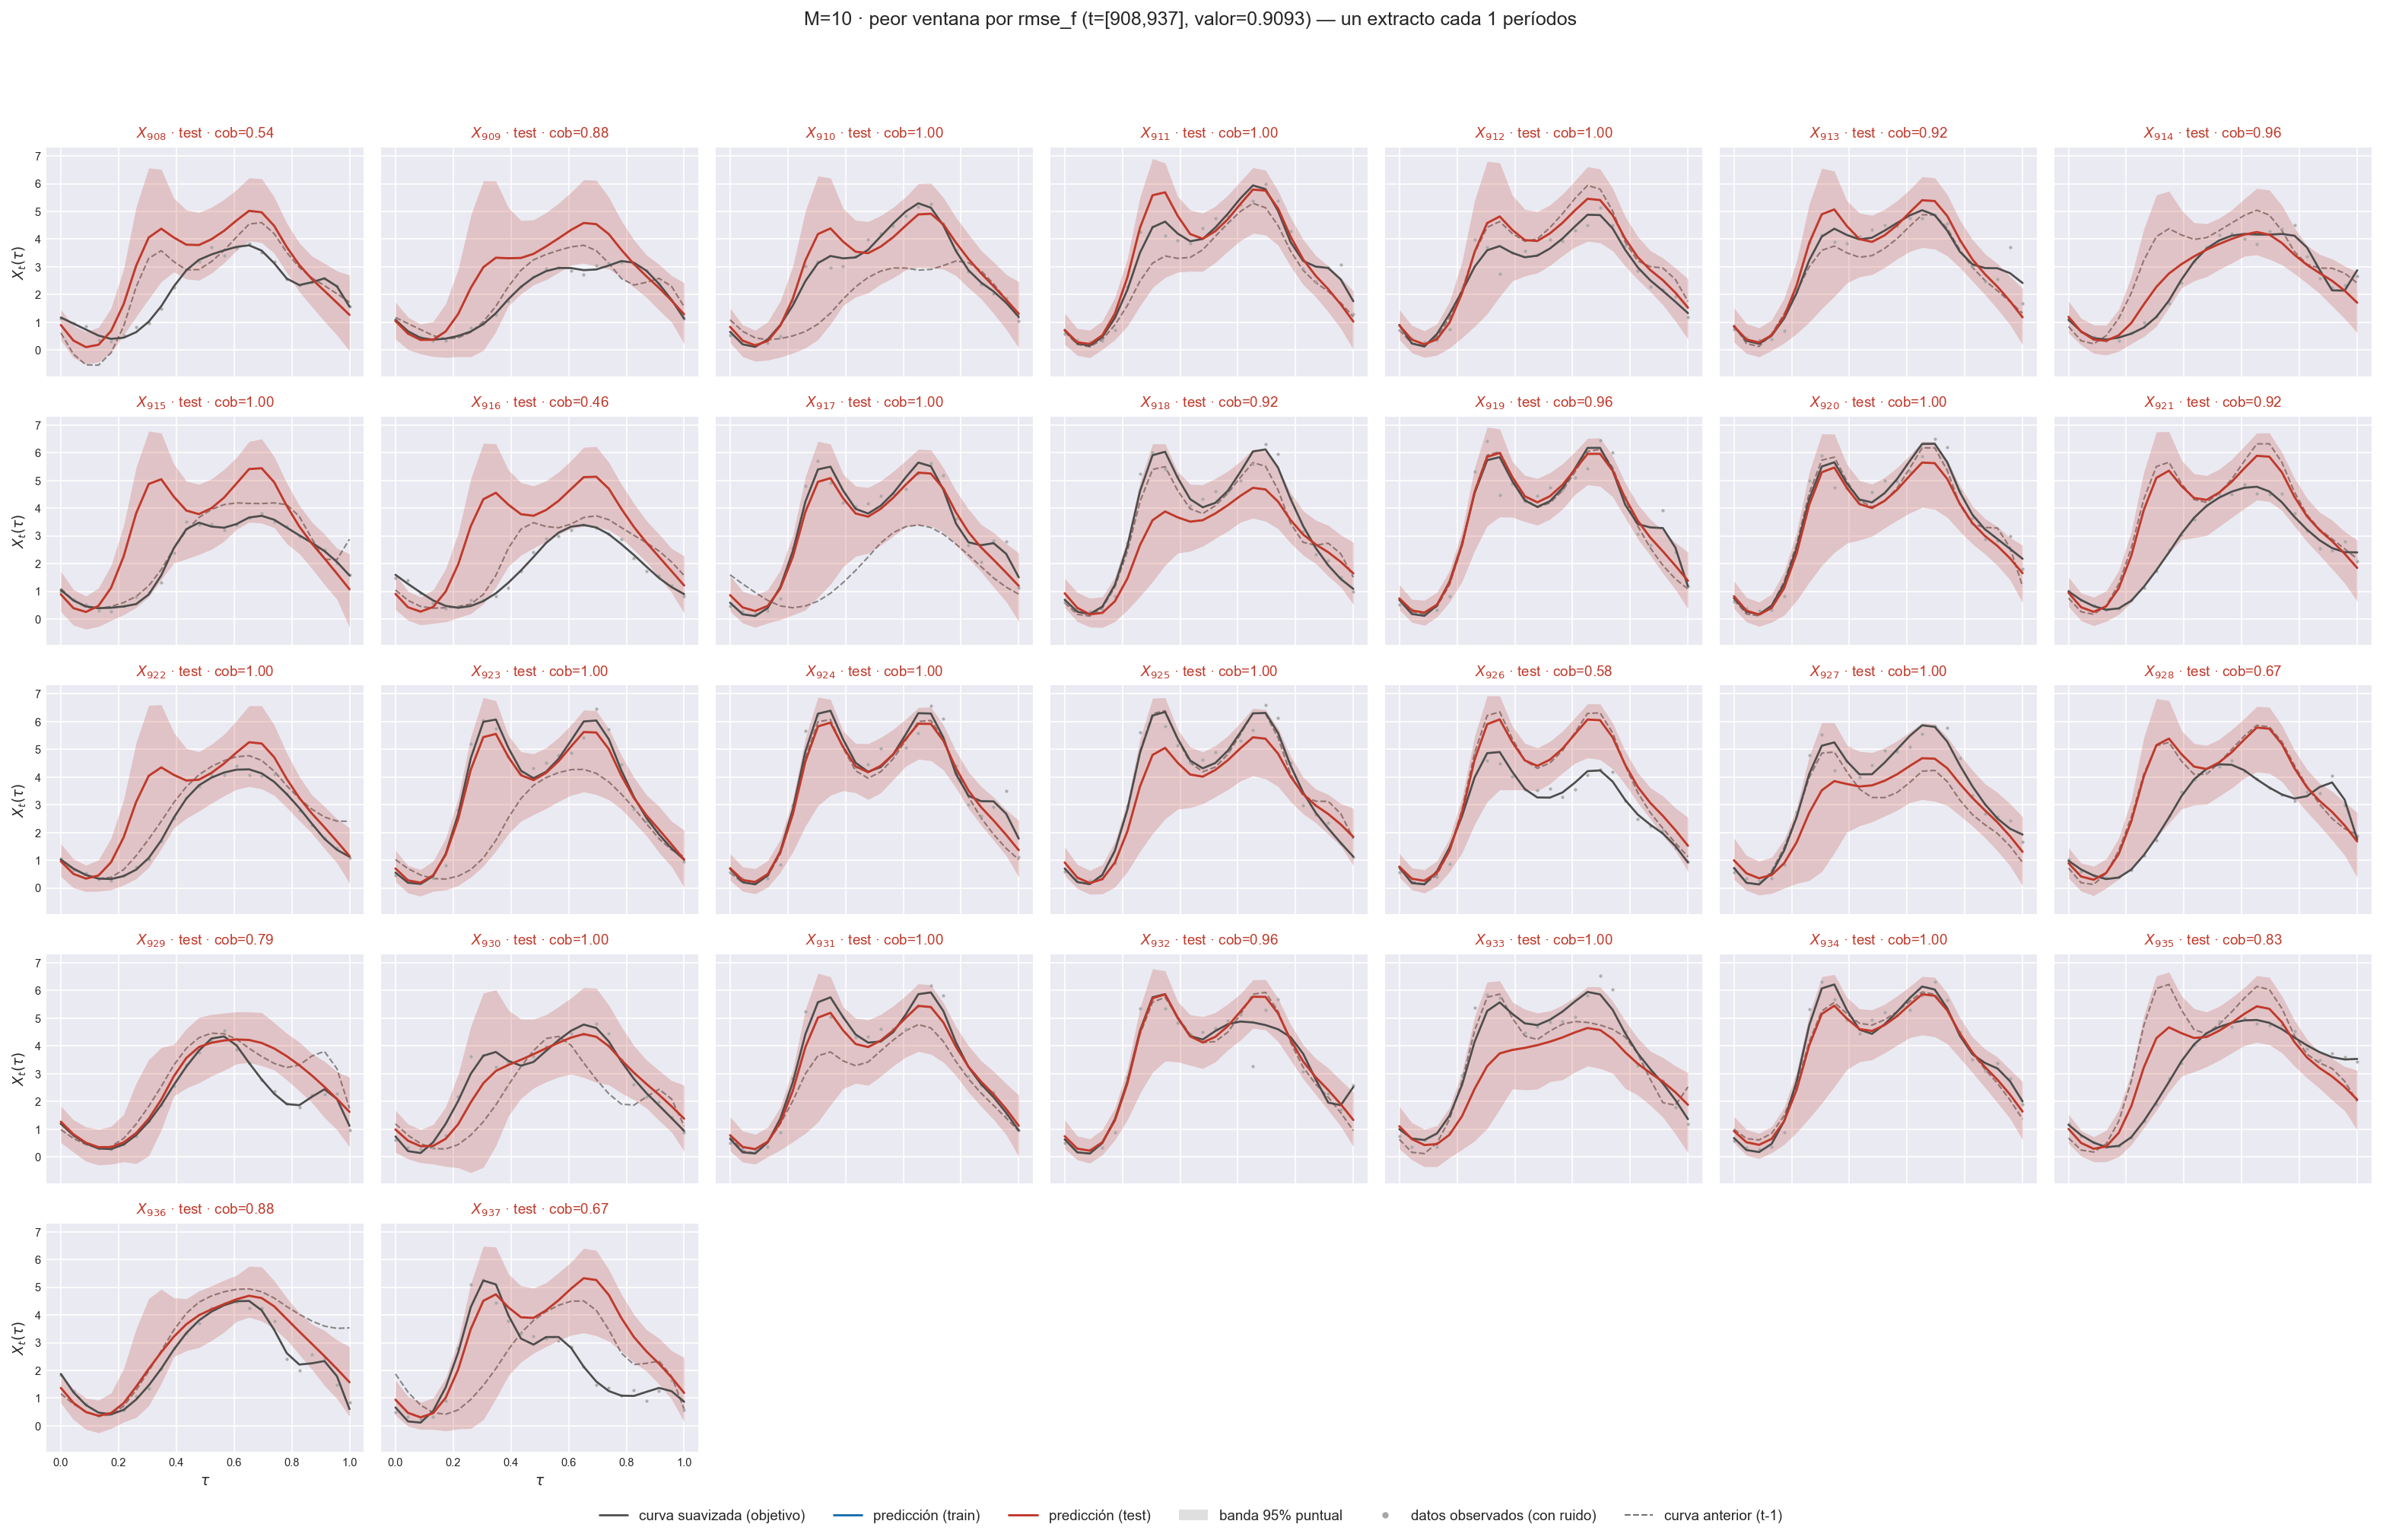
\includegraphics[width=\textwidth,height=0.8\textheight,keepaspectratio]{IMG/aneC_00/aneC_00_56b_peor_ventana_rmse_f_t908_101.png}
\caption{Ventana de peor RMSE (origen $t = 908$), tráfico con rezago $\{1\}$ ($M = 10$).}
\label{fig:aneC_56b_peor_ventana_rmse_f_t908_101}
\end{figure}

\begin{figure}[H]
\centering
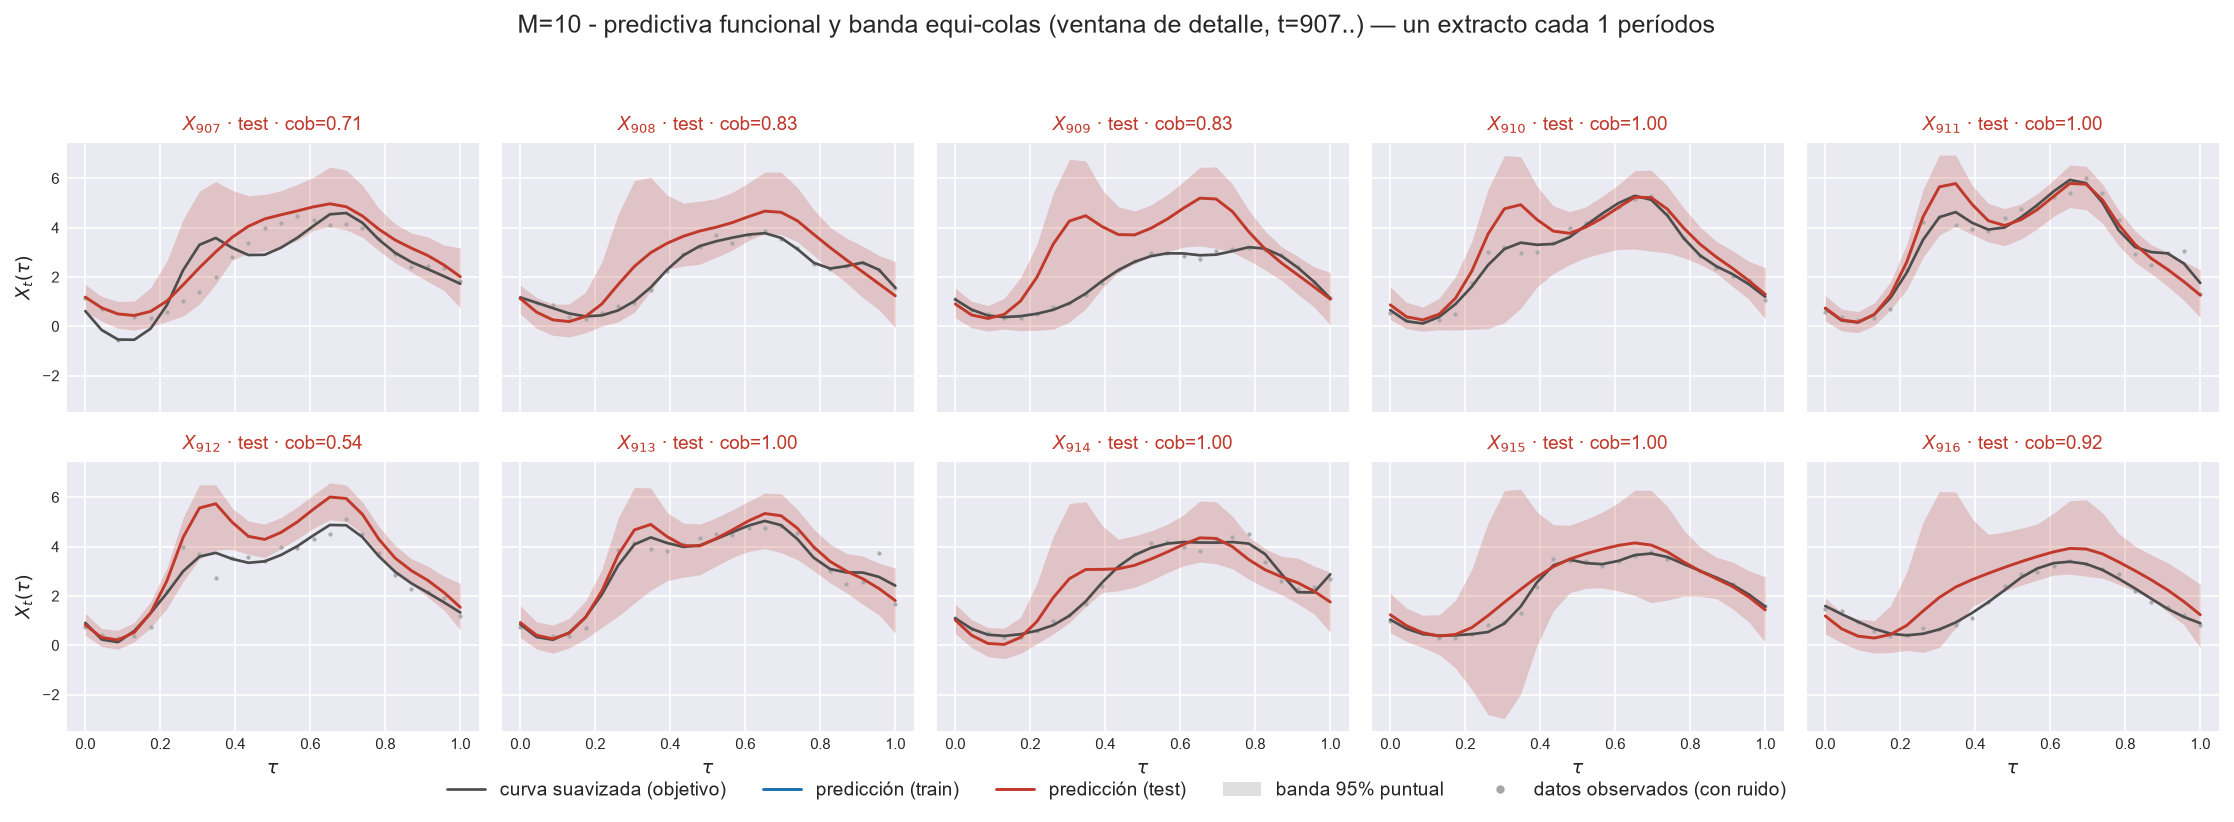
\includegraphics[width=\textwidth,height=0.8\textheight,keepaspectratio]{IMG/aneC_00/aneC_00_54_extractos_curvas_test_102.png}
\caption{Extractos de predicciones del bloque de prueba, tráfico con rezagos $\{1,7\}$ ($M = 10$).}
\label{fig:aneC_54_extractos_curvas_test_102}
\end{figure}

\begin{figure}[H]
\centering
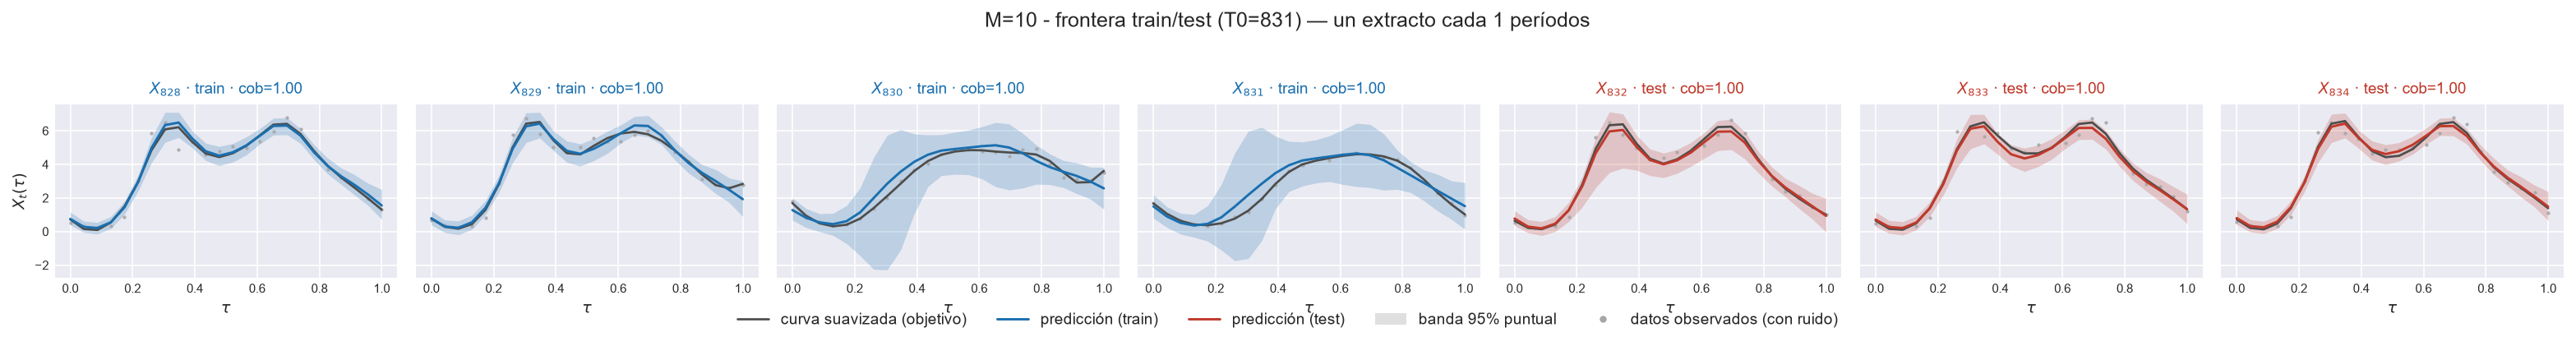
\includegraphics[width=\textwidth,height=0.8\textheight,keepaspectratio]{IMG/aneC_00/aneC_00_55_extractos_frontera_102.png}
\caption{Predicciones en la frontera entre los bloques de entrenamiento y de prueba, tráfico con rezagos $\{1,7\}$ ($M = 10$).}
\label{fig:aneC_55_extractos_frontera_102}
\end{figure}

\begin{figure}[H]
\centering
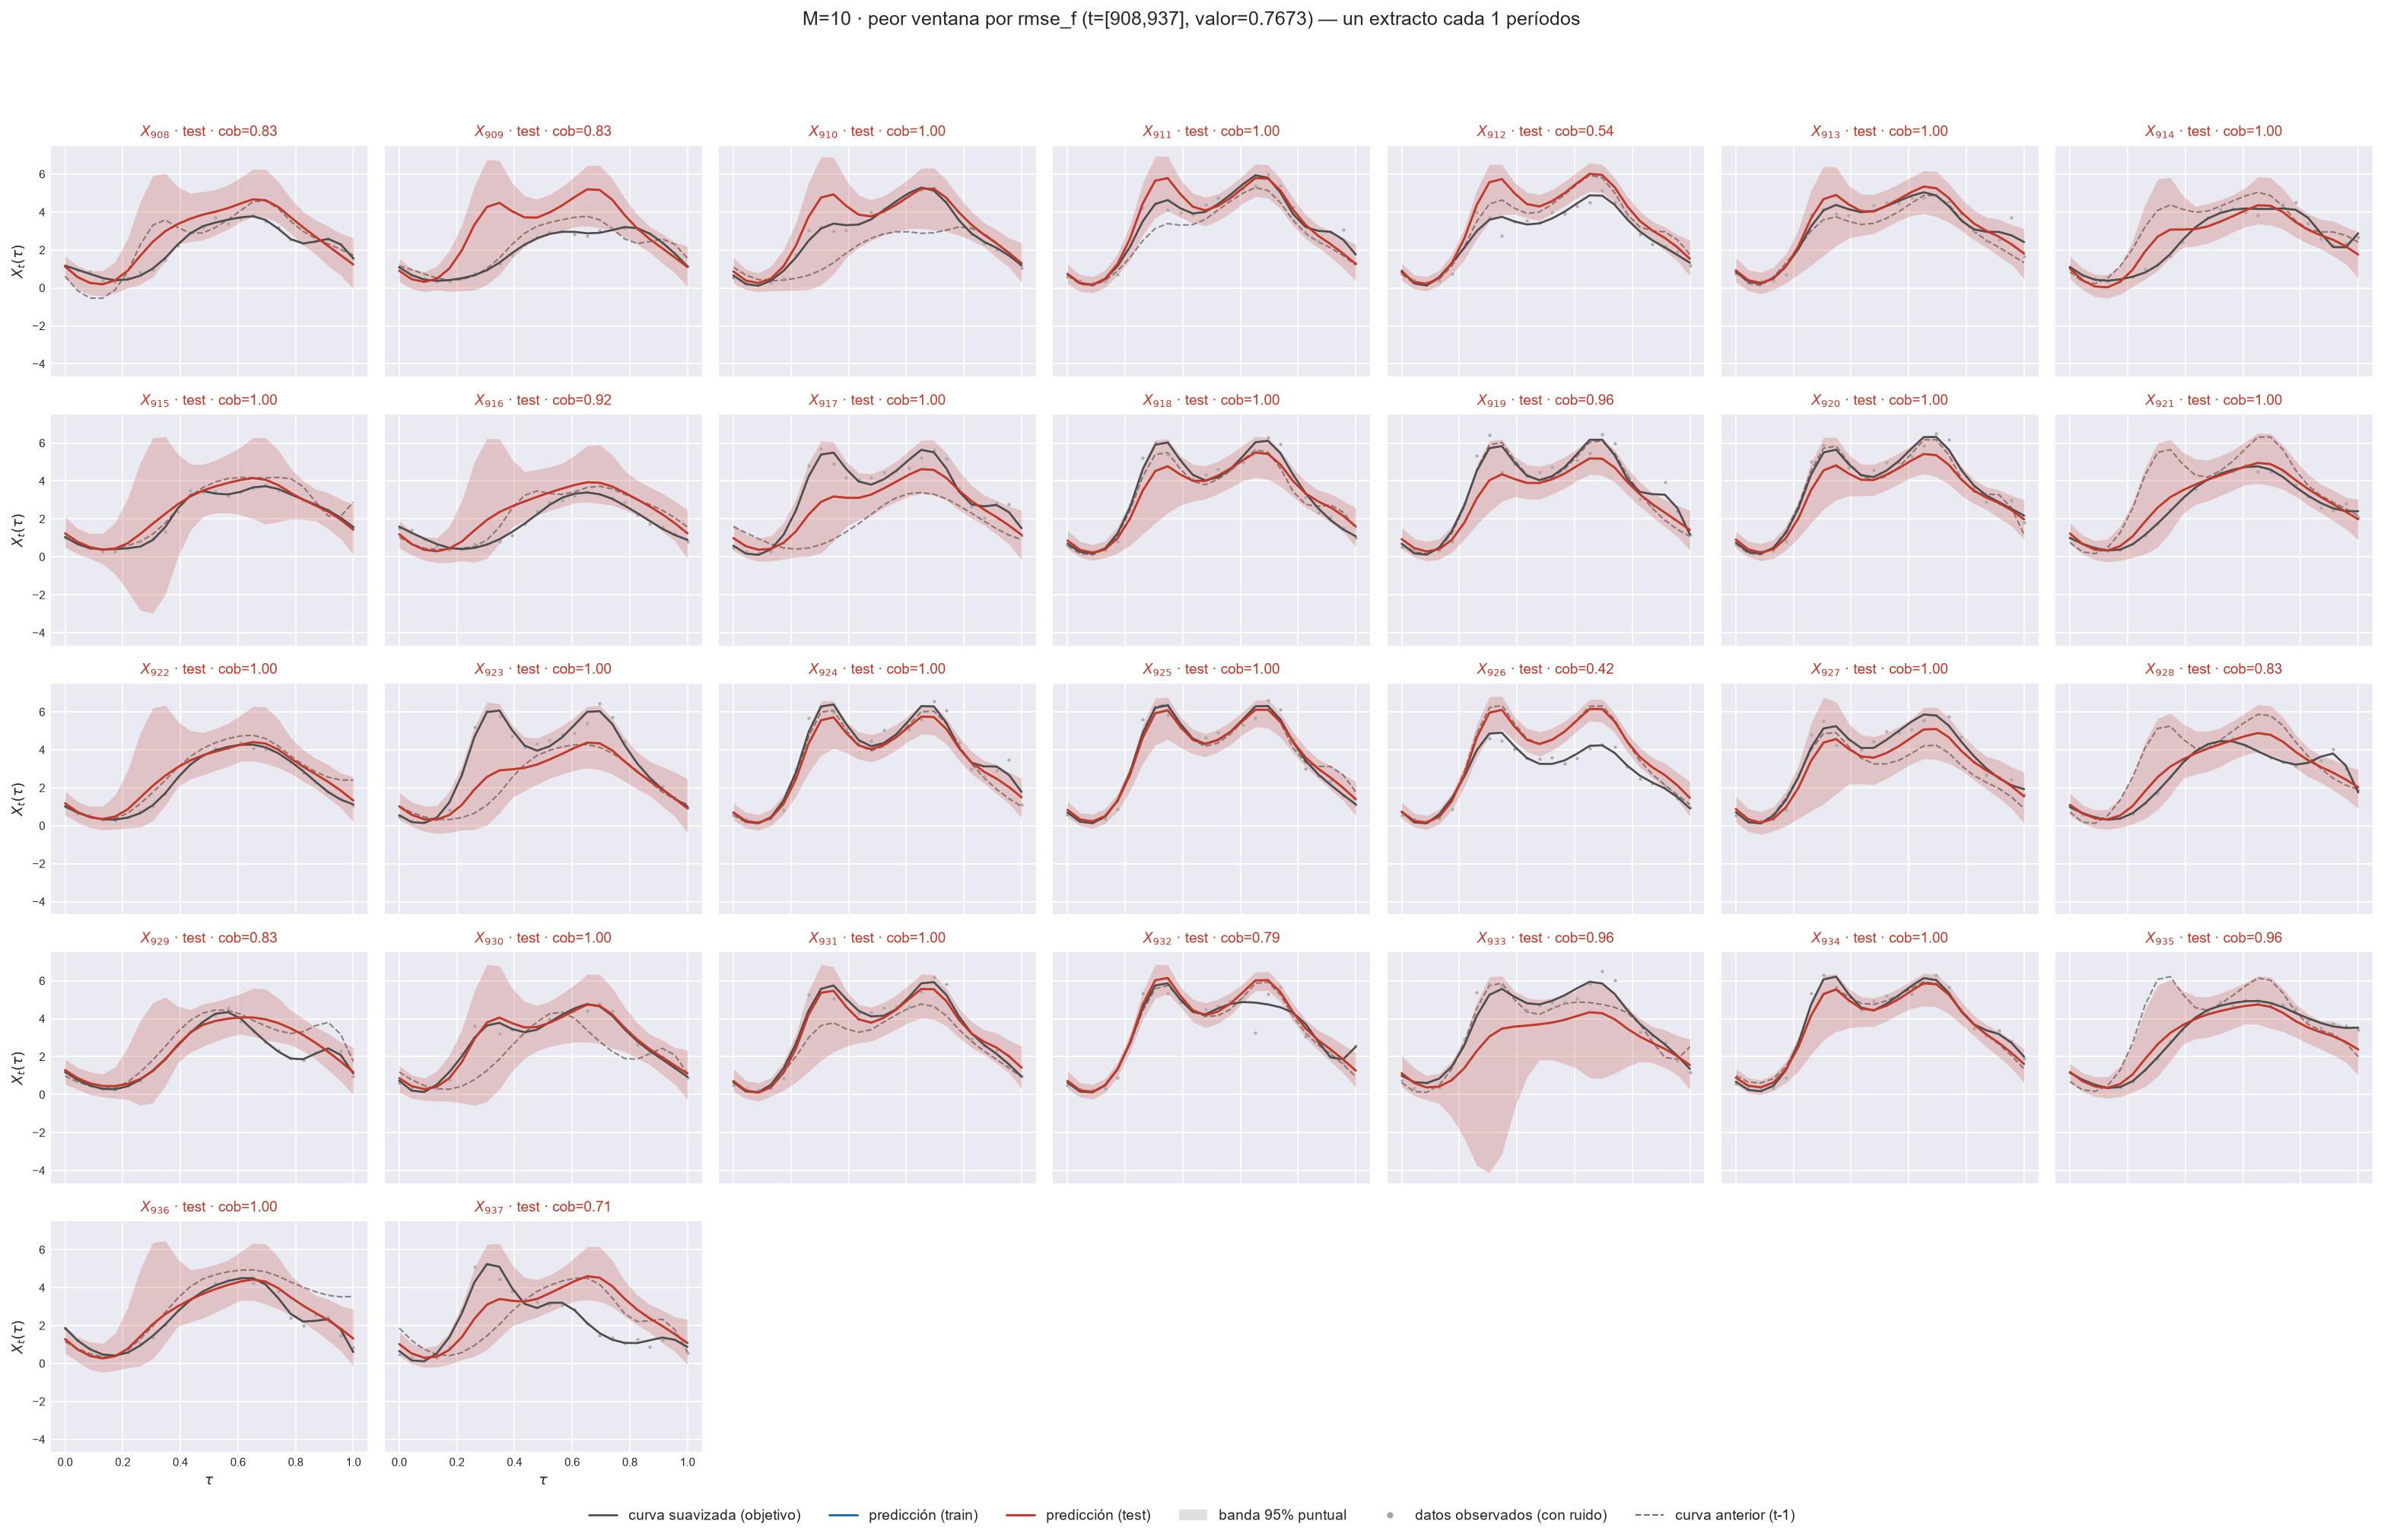
\includegraphics[width=\textwidth,height=0.8\textheight,keepaspectratio]{IMG/aneC_00/aneC_00_56b_peor_ventana_rmse_f_t908_102.png}
\caption{Ventana de peor RMSE (origen $t = 908$), tráfico con rezagos $\{1,7\}$ ($M = 10$).}
\label{fig:aneC_56b_peor_ventana_rmse_f_t908_102}
\end{figure}

\begin{figure}[H]
\centering
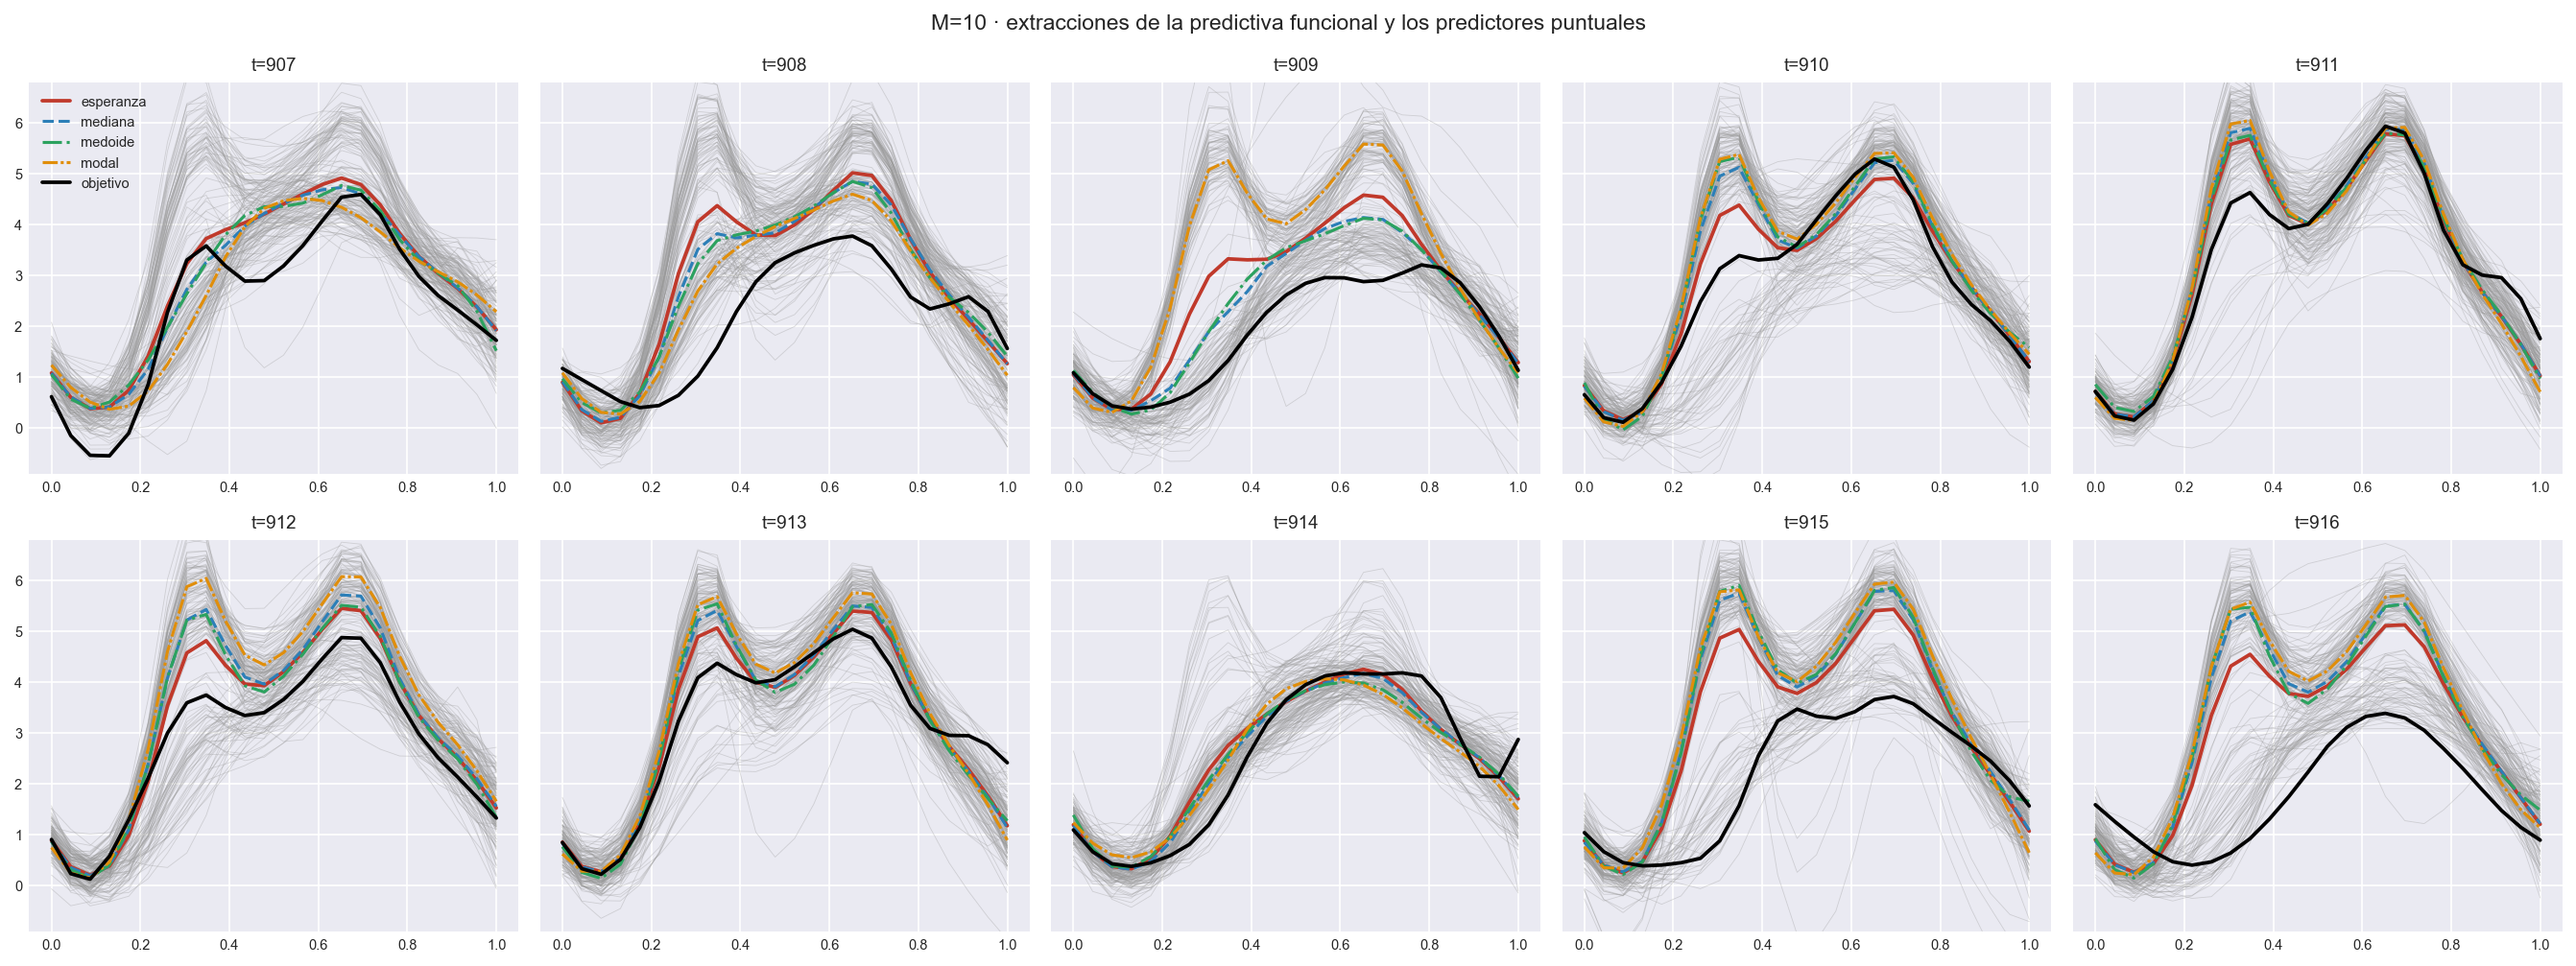
\includegraphics[width=\textwidth]{IMG/aneC_00/aneC_00_61b_curvas_predictores_101.png}
\caption{Esperanza, mediana puntual y átomo más probable en cuatro orígenes de la ventana de detalle, con la banda equi-colas y la curva observada, tráfico con rezago $\{1\}$ ($M = 10$).}
\label{fig:aneC_predictores_101}
\end{figure}

\begin{figure}[H]
\centering
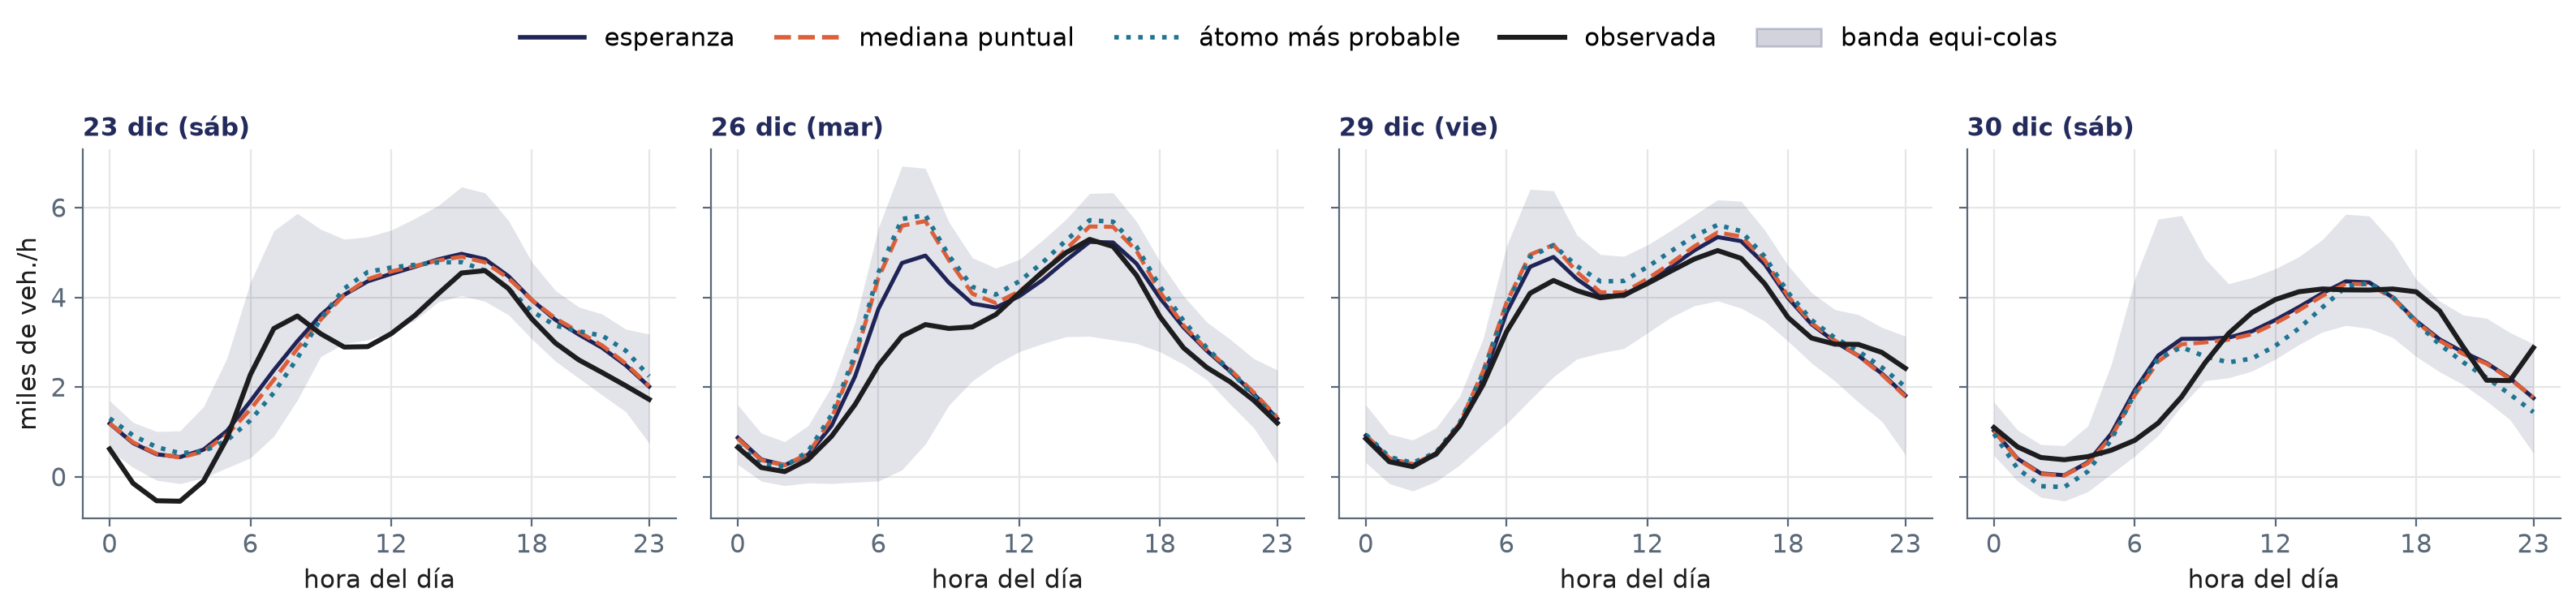
\includegraphics[width=\textwidth]{IMG/aneC_00/aneC_00_61b_curvas_predictores_102.png}
\caption{Esperanza, mediana puntual y átomo más probable en cuatro orígenes de la ventana de detalle, con la banda equi-colas y la curva observada, tráfico con rezagos $\{1,7\}$ ($M = 10$).}
\label{fig:aneC_predictores_102}
\end{figure}

\section{Comportamientos predictivos}
\label{aneC_00_06_comportamientos}

Esta sección complementa la Sección~\ref{04_03_03_comportamientos}: el número de comportamientos a lo largo del bloque de prueba, su transición entre especificaciones, los feriados, las extracciones y el catálogo de comportamientos, y los diez orígenes de la ventana de detalle.

% Fuente: K de comportamientos_psbp.npz y calendario de 65_comportamientos_calendario.csv (test).
\begin{figure}[H]
\centering
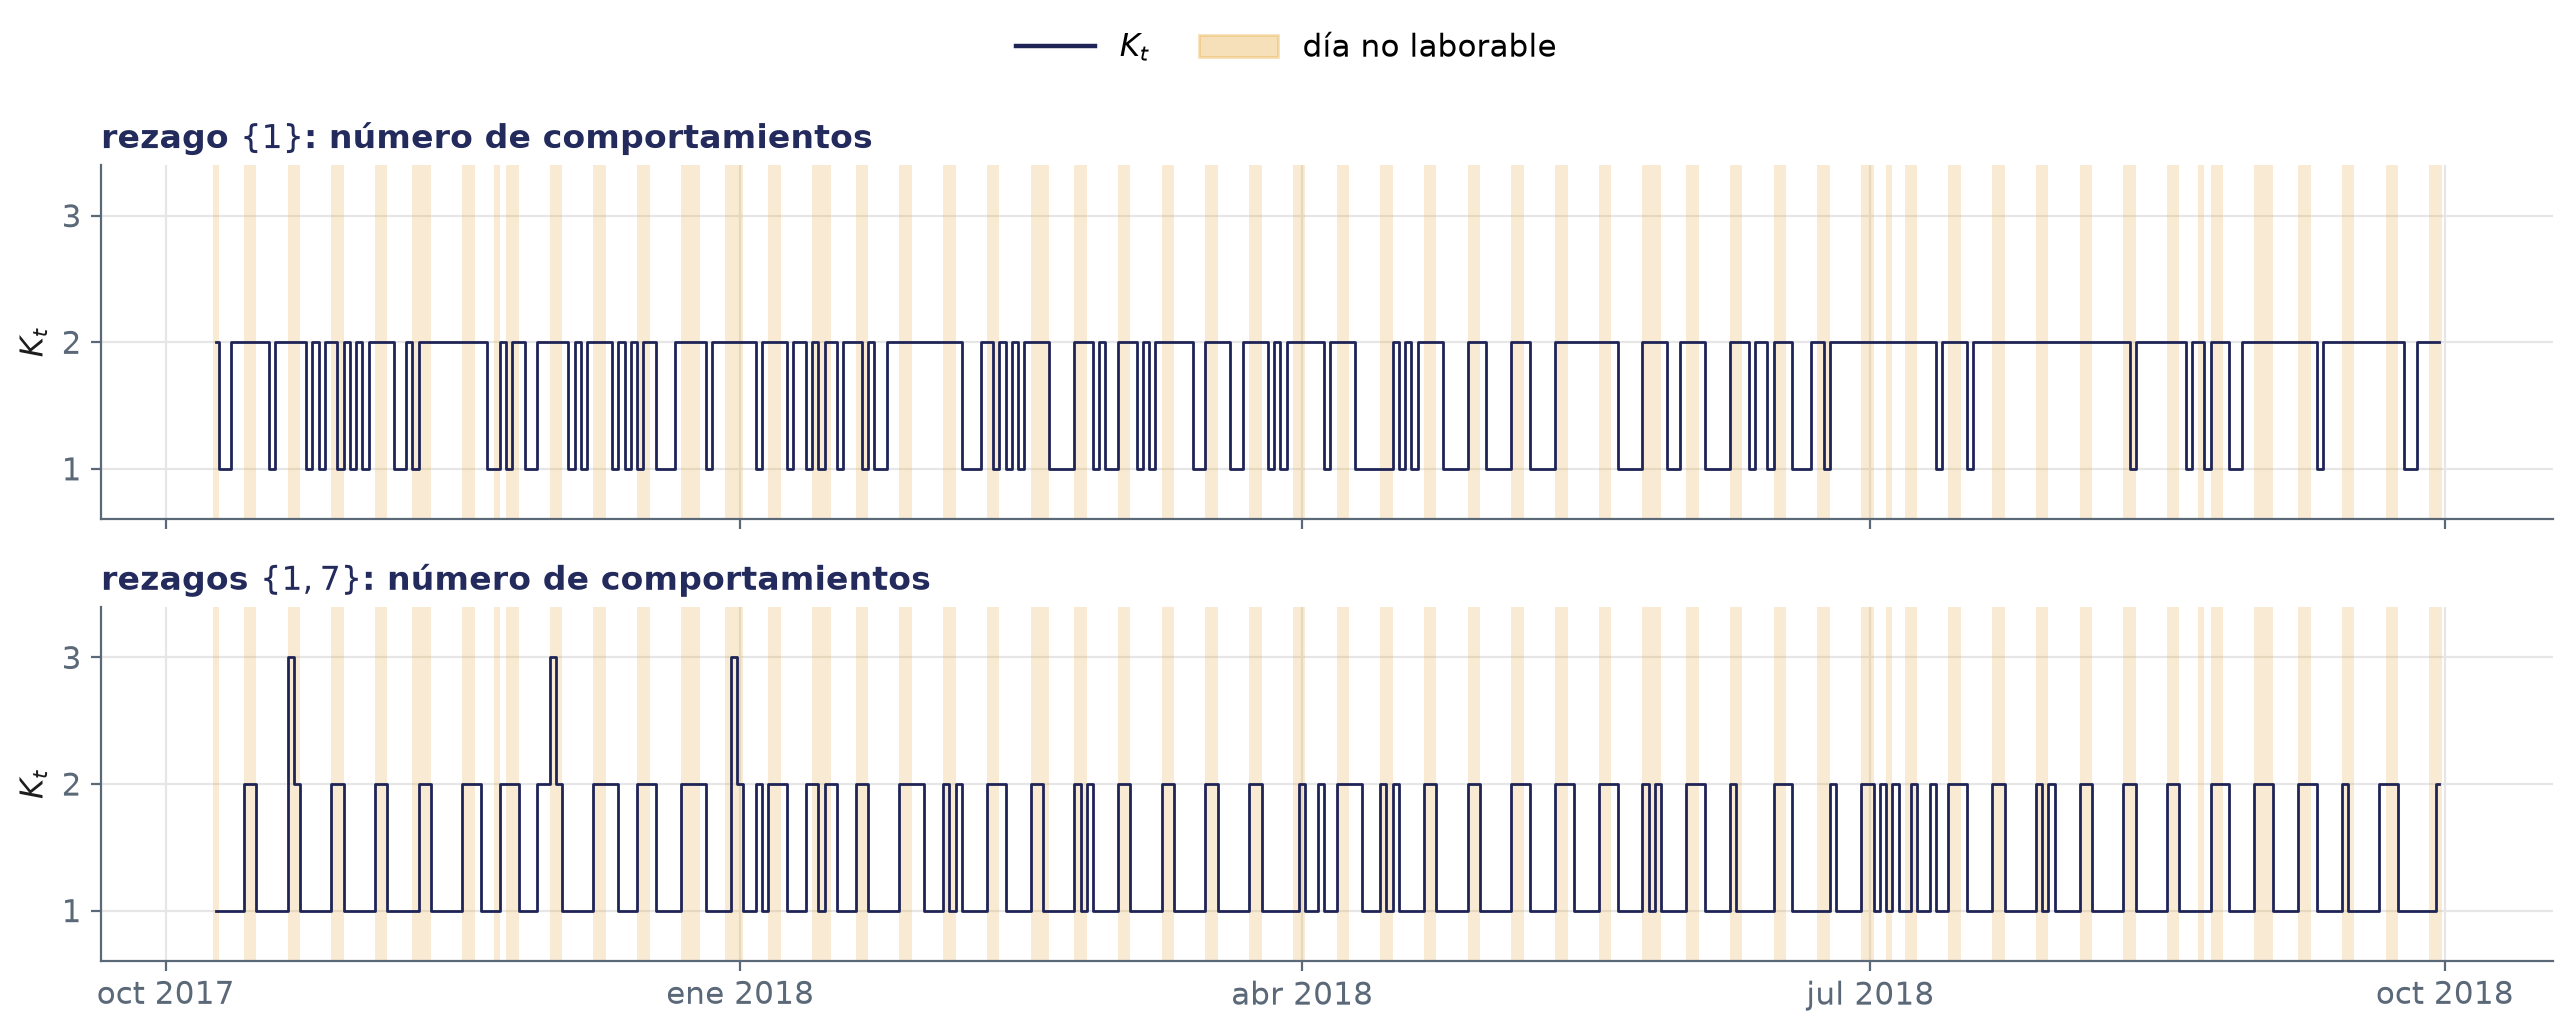
\includegraphics[width=\textwidth]{IMG/aneC_00/aneC_00_102b_K_serie.png}
\caption{Número de comportamientos $K_t$ en cada origen de prueba, con los días no laborables marcados, con rezago $\{1\}$ (arriba) y rezagos $\{1,7\}$ (abajo) ($M = 10$).}
\label{fig:aneC_Kserie}
\end{figure}

El Cuadro~\ref{tab:aneC_transicion} cruza el número de comportamientos de cada origen de prueba en las dos especificaciones. De los 256 orígenes con dos comportamientos con el rezago de un día, 139 pasan a tener uno solo al agregar el rezago semanal y 114 los conservan, mientras que solo 11 de los 101 orígenes con un comportamiento ganan un segundo.

% Fuente: K de comportamientos_psbp.npz de 101 y 102 (test, mismos 357 orígenes).
\begin{table}[H]
\centering\small
\caption{Número de comportamientos por origen de prueba con rezago $\{1\}$ (filas) y con rezagos $\{1,7\}$ (columnas) ($M = 10$).}
\label{tab:aneC_transicion}
\begin{tabular}{l ccc c}
\hline
 & $K_t = 1$ & $K_t = 2$ & $K_t = 3$ & Total \\
\hline
$K_t = 1$ & 90  & 11  & 0 & 101 \\
$K_t = 2$ & 139 & 114 & 3 & 256 \\
\hline
Total     & 229 & 125 & 3 & 357 \\
\hline
\end{tabular}
\end{table}

El Cuadro~\ref{tab:aneC_feriados} muestra el número de comportamientos en los once feriados del bloque de prueba. Con el rezago de un día nueve de ellos tienen dos comportamientos. Con el rezago semanal conservan dos comportamientos cinco feriados, todos en lunes, y pasan a uno los dos de mitad de semana y dos lunes; un solo comportamiento no implica que el perfil sea el correcto, porque en esos días la semana anterior anuncia un día laborable.

% Fuente: 65_comportamientos_calendario.csv y K de comportamientos_psbp.npz de 101 y 102.
\begin{table}[H]
\centering\small
\caption{Número de comportamientos en los feriados del bloque de prueba ($M = 10$).}
\label{tab:aneC_feriados}
\begin{tabular}{l l l cc}
\hline
Fecha & Día & Feriado & $\{1\}$ & $\{1,7\}$ \\
\hline
9 oct 2017  & lunes     & Columbus Day              & 2 & 1 \\
10 nov 2017 & viernes   & Veterans Day              & 1 & 1 \\
23 nov 2017 & jueves    & Thanksgiving Day          & 1 & 1 \\
25 dic 2017 & lunes     & Christmas Day             & 2 & 2 \\
1 ene 2018  & lunes     & New Year's Day            & 2 & 2 \\
15 ene 2018 & lunes     & Martin Luther King Jr Day & 2 & 2 \\
19 feb 2018 & lunes     & Washington's Birthday     & 2 & 1 \\
28 may 2018 & lunes     & Memorial Day              & 2 & 2 \\
4 jul 2018  & miércoles & Independence Day          & 2 & 1 \\
23 ago 2018 & jueves    & State Fair                & 2 & 1 \\
3 sep 2018  & lunes     & Labor Day                 & 2 & 2 \\
\hline
\end{tabular}
\end{table}

\begin{figure}[H]
\centering
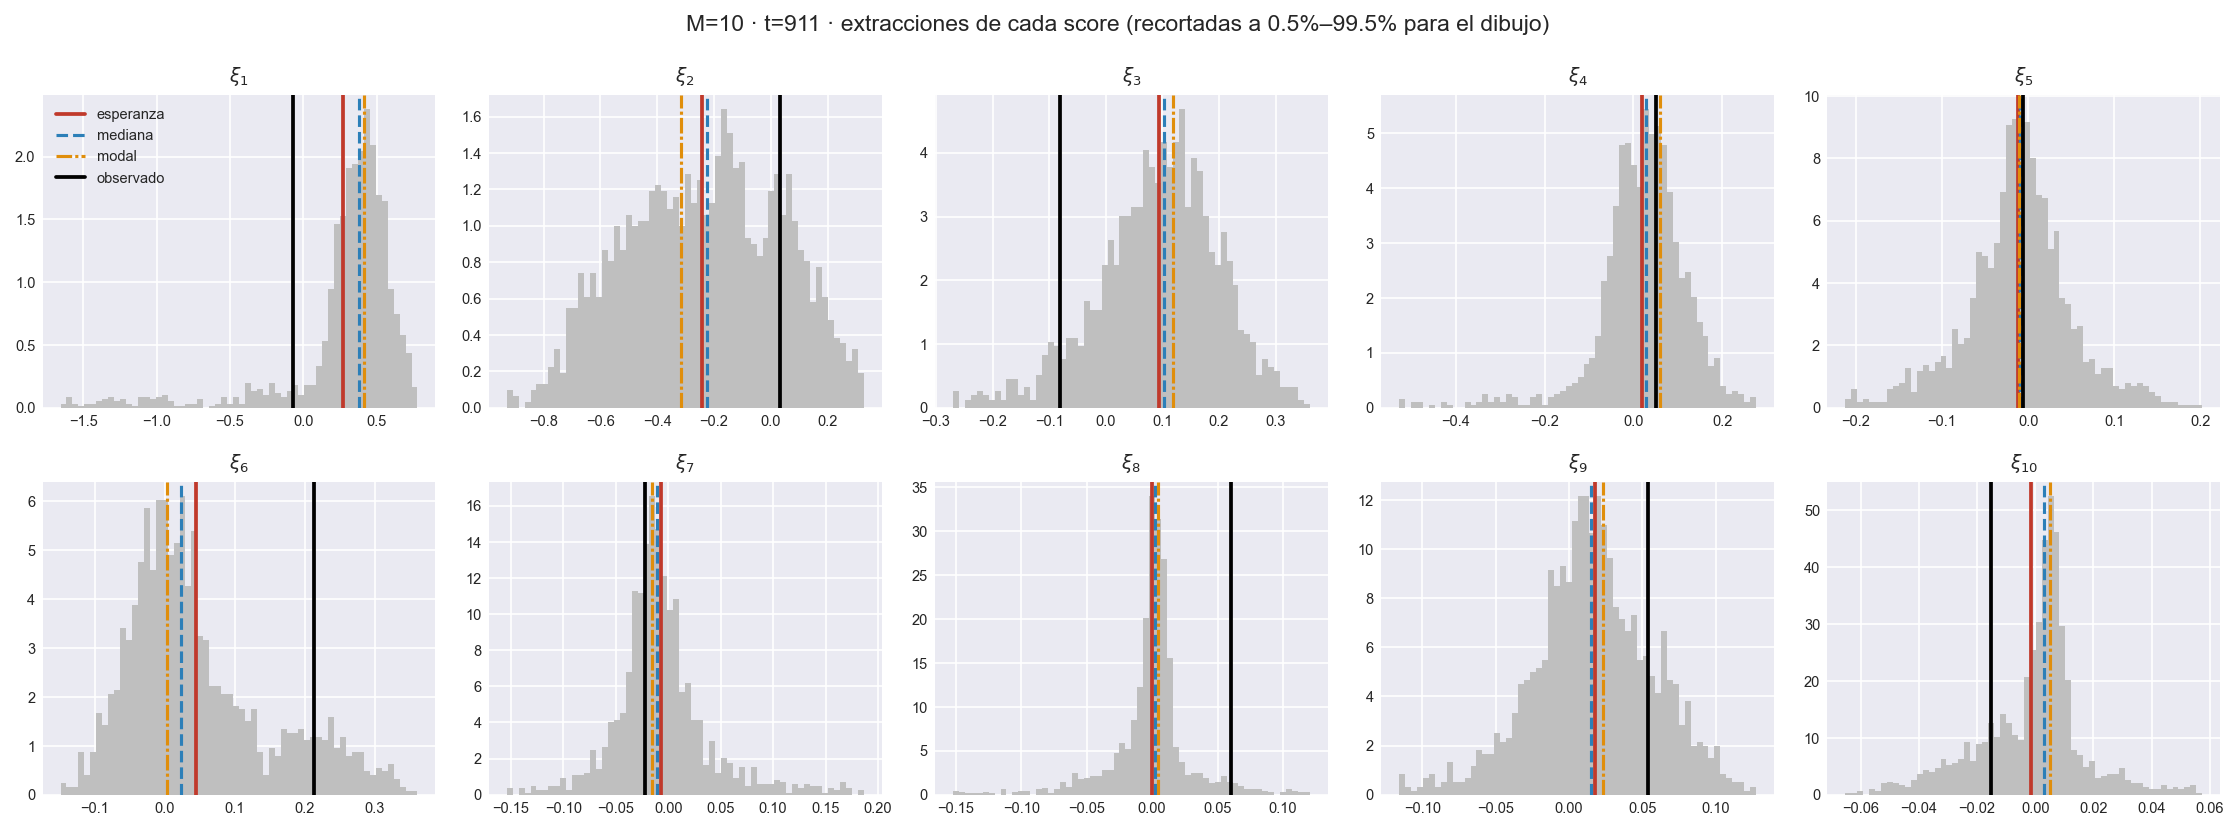
\includegraphics[width=\textwidth,height=0.6\textheight,keepaspectratio]{IMG/aneC_00/aneC_00_61_histogramas_draws_101.png}
\caption{Histograma de las extracciones del score en un origen con más de un comportamiento, tráfico con rezago $\{1\}$ ($M = 10$).}
\label{fig:aneC_hist_101}
\end{figure}

\begin{figure}[H]
\centering
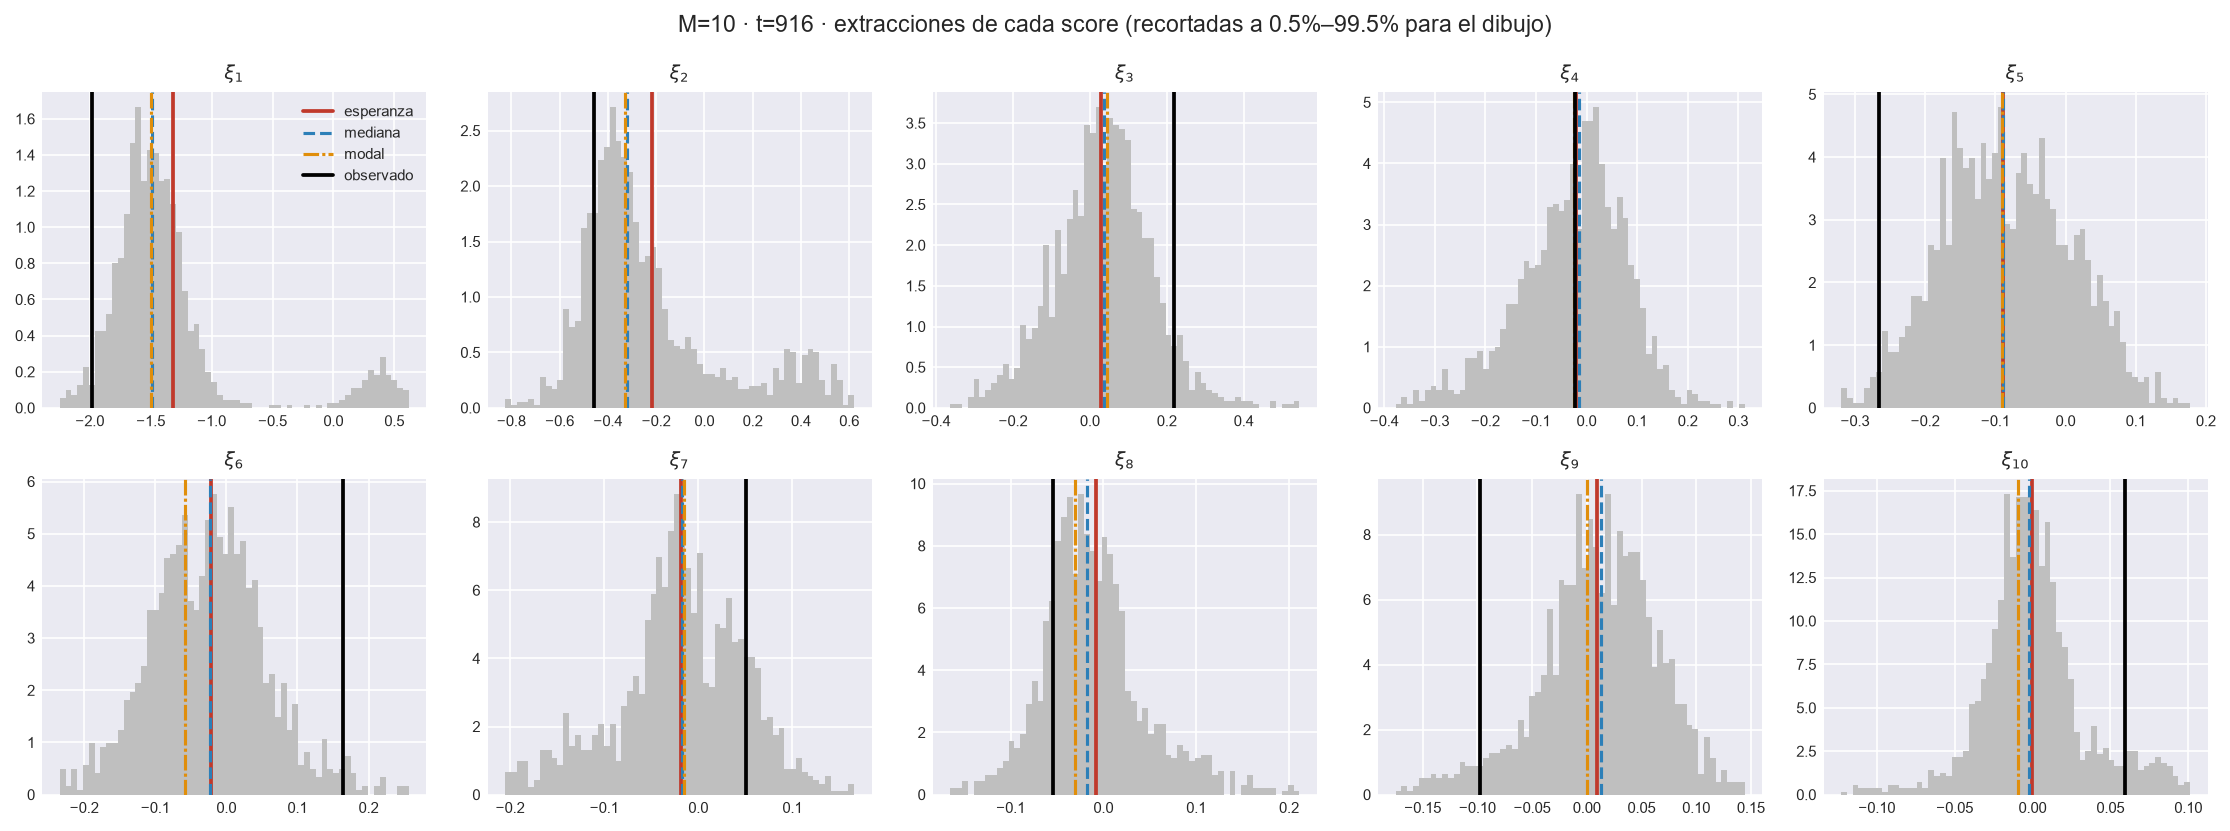
\includegraphics[width=\textwidth,height=0.6\textheight,keepaspectratio]{IMG/aneC_00/aneC_00_61_histogramas_draws_102.png}
\caption{Histograma de las extracciones del score en un origen con más de un comportamiento, tráfico con rezagos $\{1,7\}$ ($M = 10$).}
\label{fig:aneC_hist_102}
\end{figure}

\begin{figure}[H]
\centering
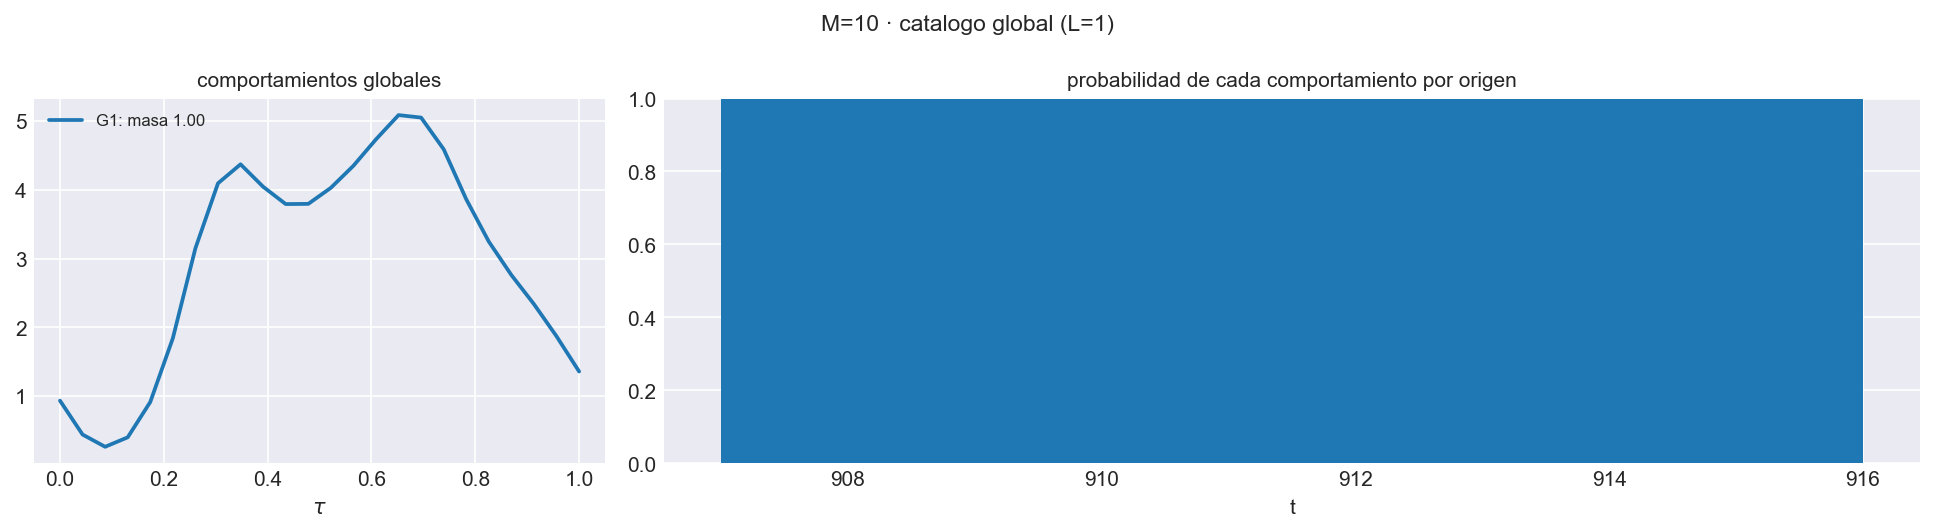
\includegraphics[width=\textwidth,height=0.6\textheight,keepaspectratio]{IMG/aneC_00/aneC_00_64_catalogo_global_101.png}
\caption{Catálogo global de comportamientos, tráfico con rezago $\{1\}$ ($M = 10$).}
\label{fig:aneC_catalogo_101}
\end{figure}

\begin{figure}[H]
\centering
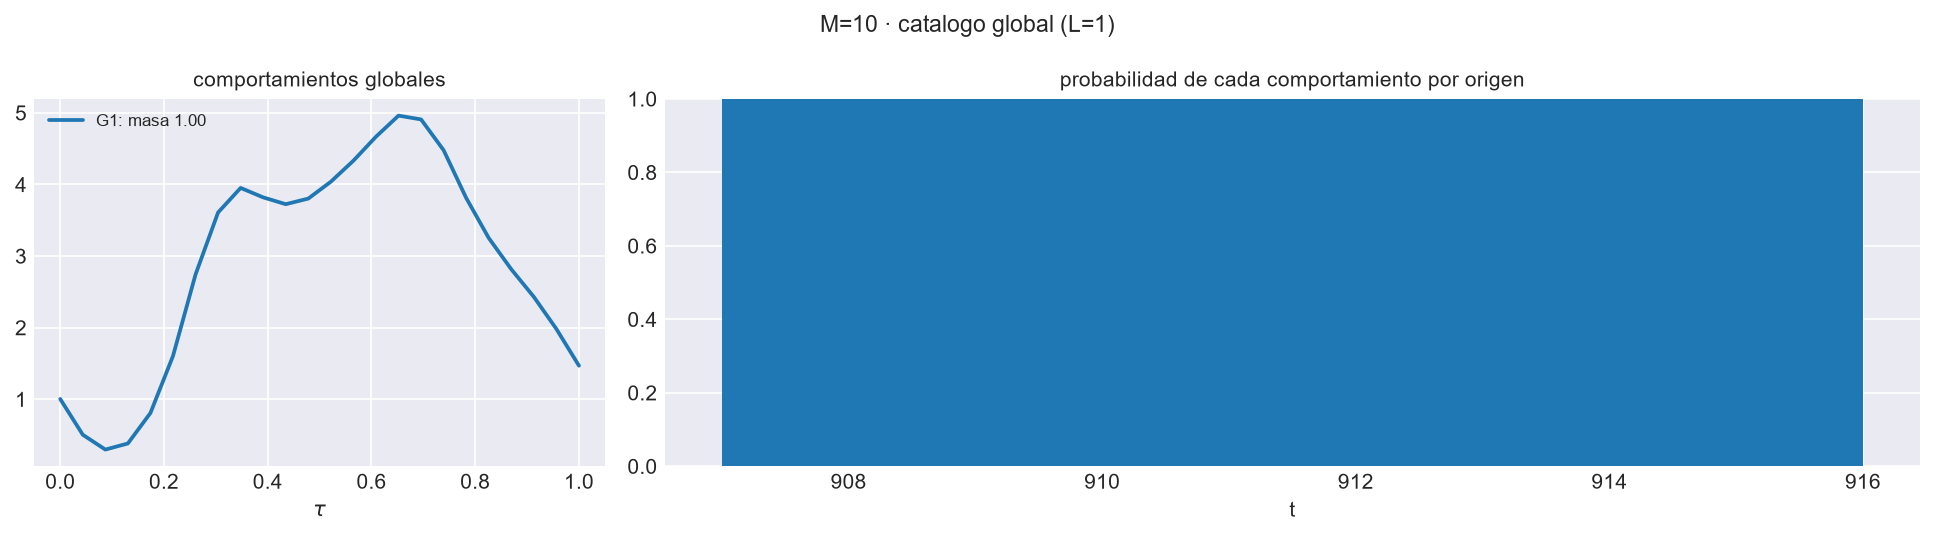
\includegraphics[width=\textwidth,height=0.6\textheight,keepaspectratio]{IMG/aneC_00/aneC_00_64_catalogo_global_102.png}
\caption{Catálogo global de comportamientos, tráfico con rezagos $\{1,7\}$ ($M = 10$).}
\label{fig:aneC_catalogo_102}
\end{figure}

% Fuente: comportamientos_psbp.npz y banda_funcional_psbp.npz del _04 de 101 y 102, curva suavizada (theta @ phi^T).
\begin{figure}[H]
\centering
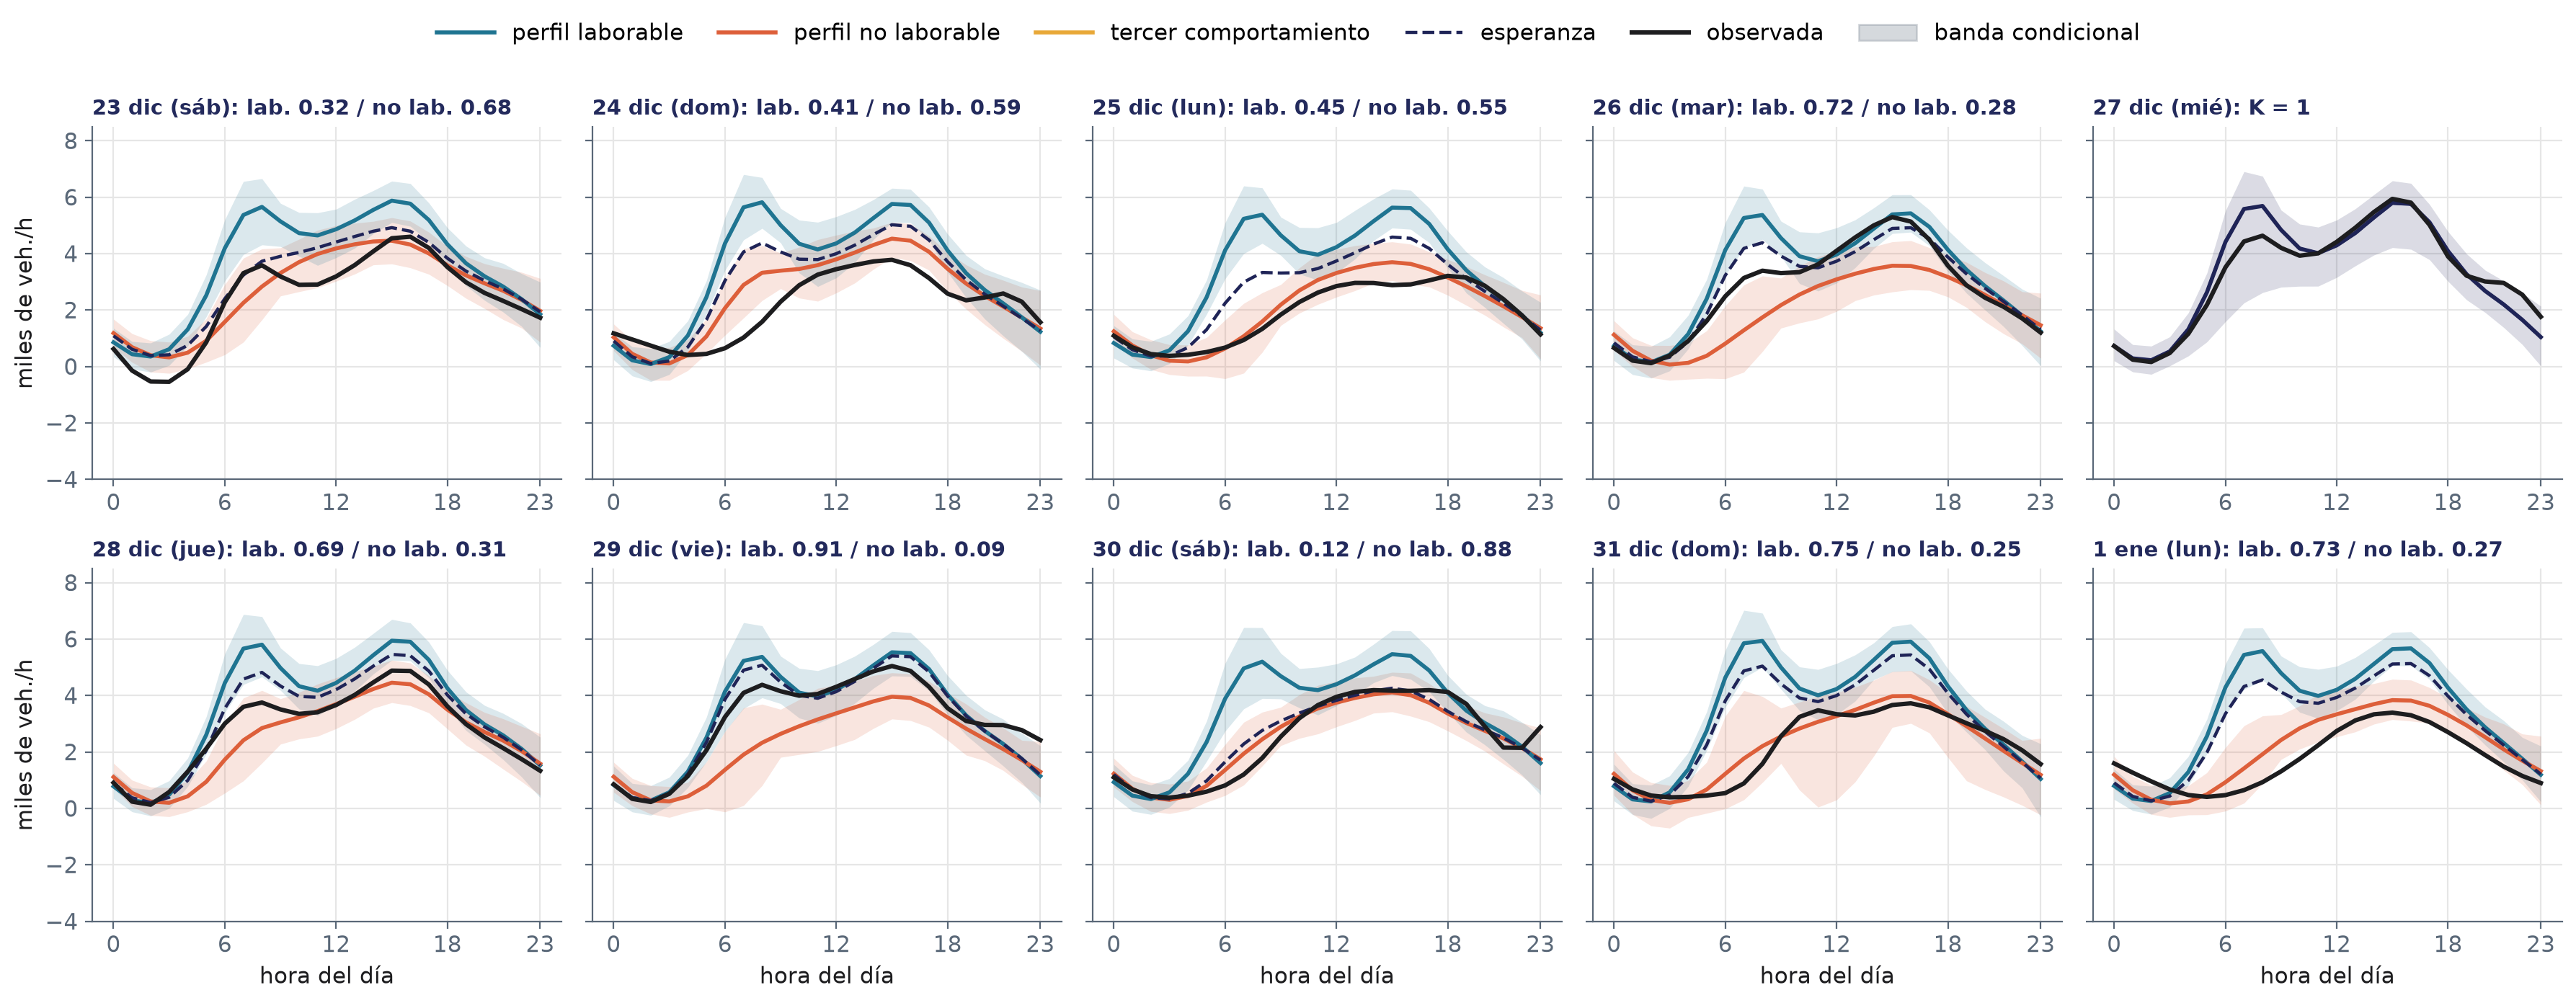
\includegraphics[width=\textwidth]{IMG/aneC_00/aneC_00_63_detalle_101.png}
\caption{Ventana de detalle completa, del 23 de diciembre de 2017 al 1 de enero de 2018, tráfico con rezago $\{1\}$ ($M = 10$): curva observada, esperanza y, por comportamiento, curva típica, banda condicional y probabilidad.}
\label{fig:aneC_detalle_101}
\end{figure}

\begin{figure}[H]
\centering
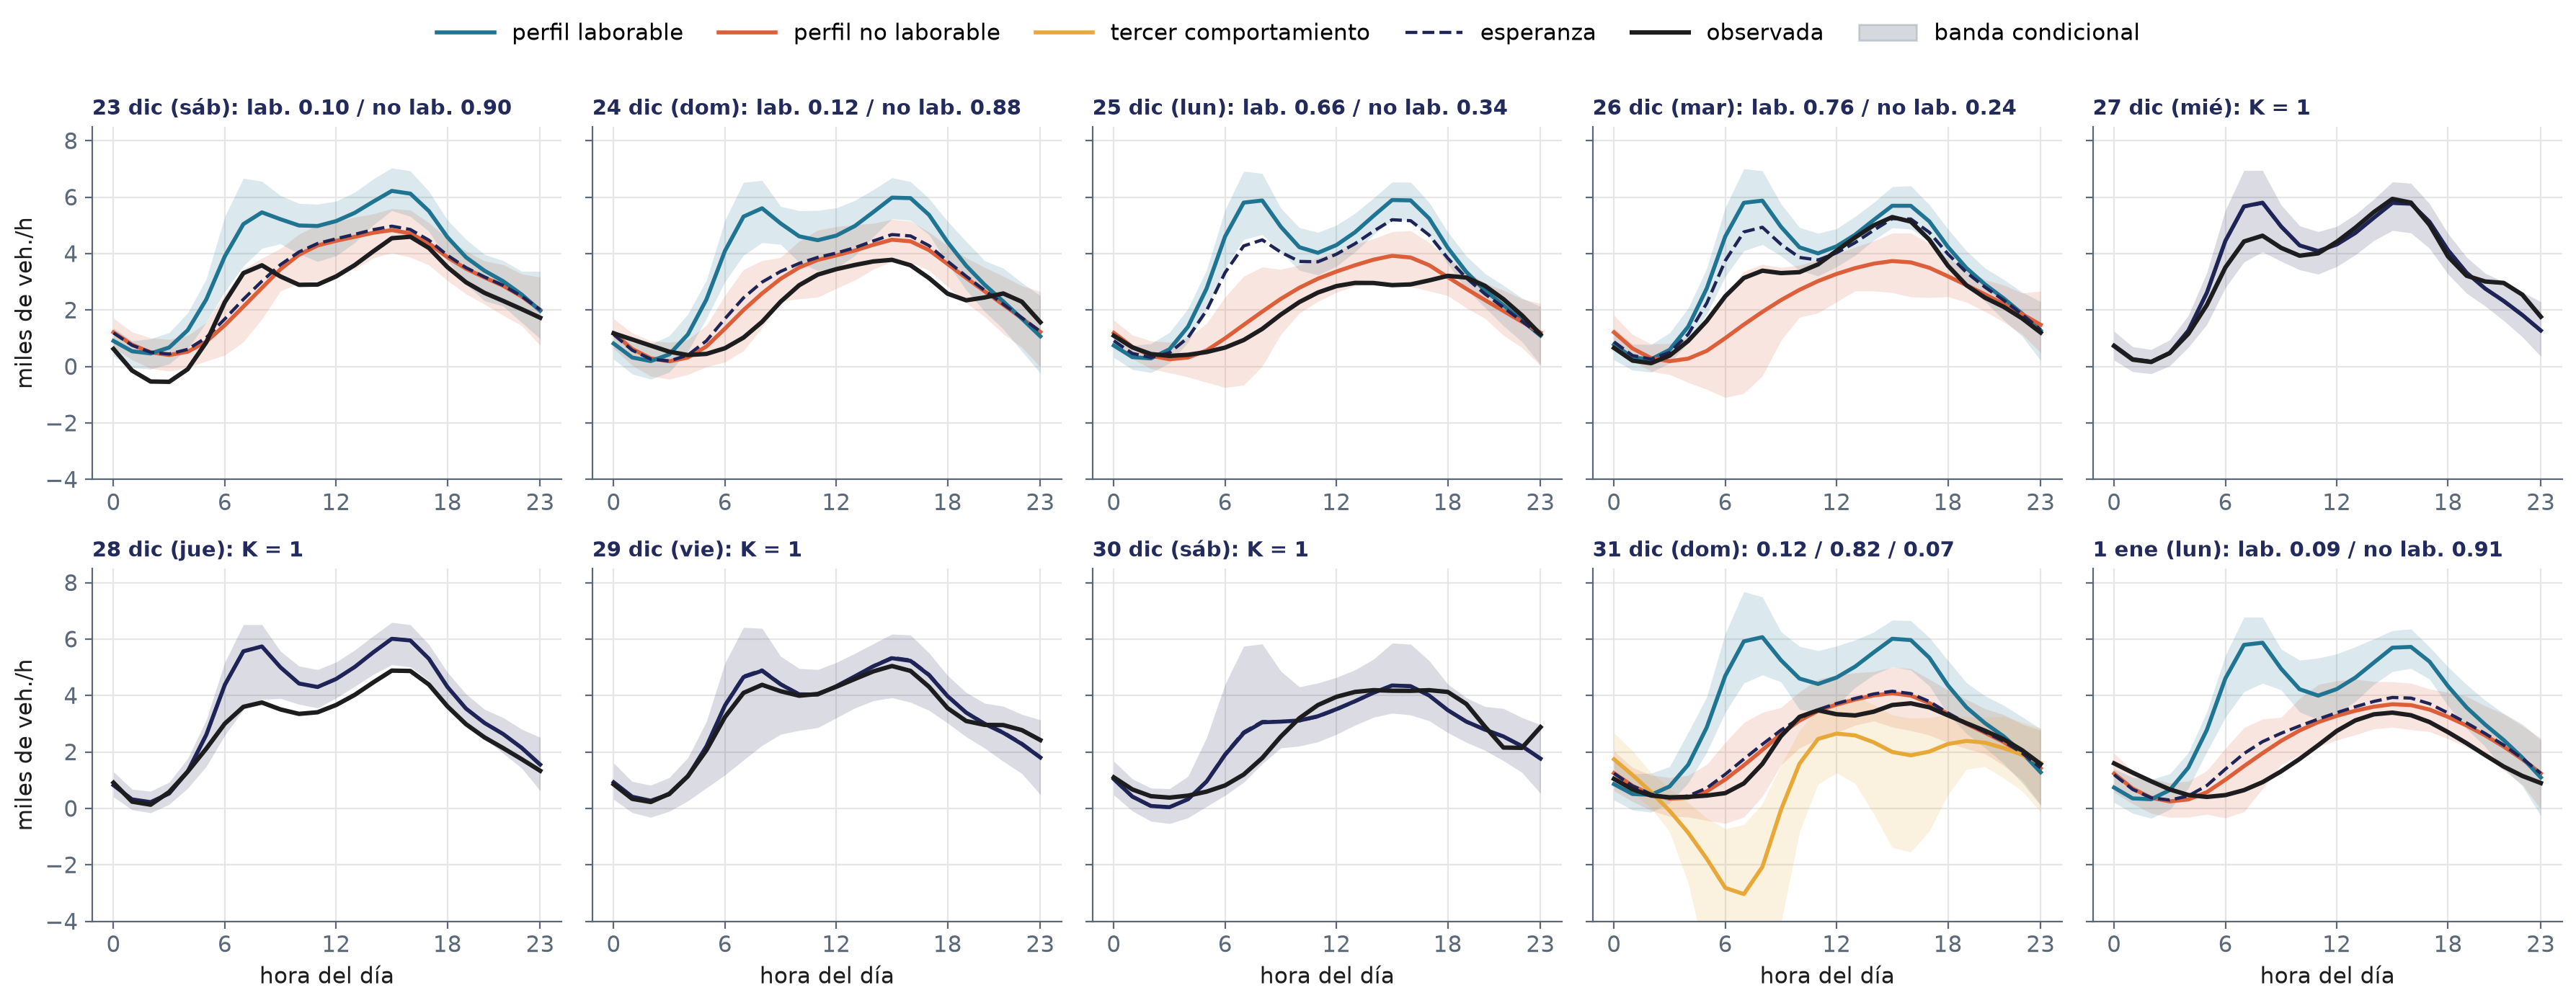
\includegraphics[width=\textwidth]{IMG/aneC_00/aneC_00_63_detalle_102.png}
\caption{Ventana de detalle completa, del 23 de diciembre de 2017 al 1 de enero de 2018, tráfico con rezagos $\{1,7\}$ ($M = 10$). Con tres comportamientos, las probabilidades van en orden de nivel.}
\label{fig:aneC_detalle_102}
\end{figure}

\section{Intervalos en la ventana de detalle}
\label{aneC_00_07_intervalos_detalle}
% 79: contraste de las bandas en la ventana de detalle.

Las tres construcciones de intervalo del PSBPM-FD y la banda del FAR en los diez orígenes de la ventana de detalle.

\begin{figure}[H]
\centering
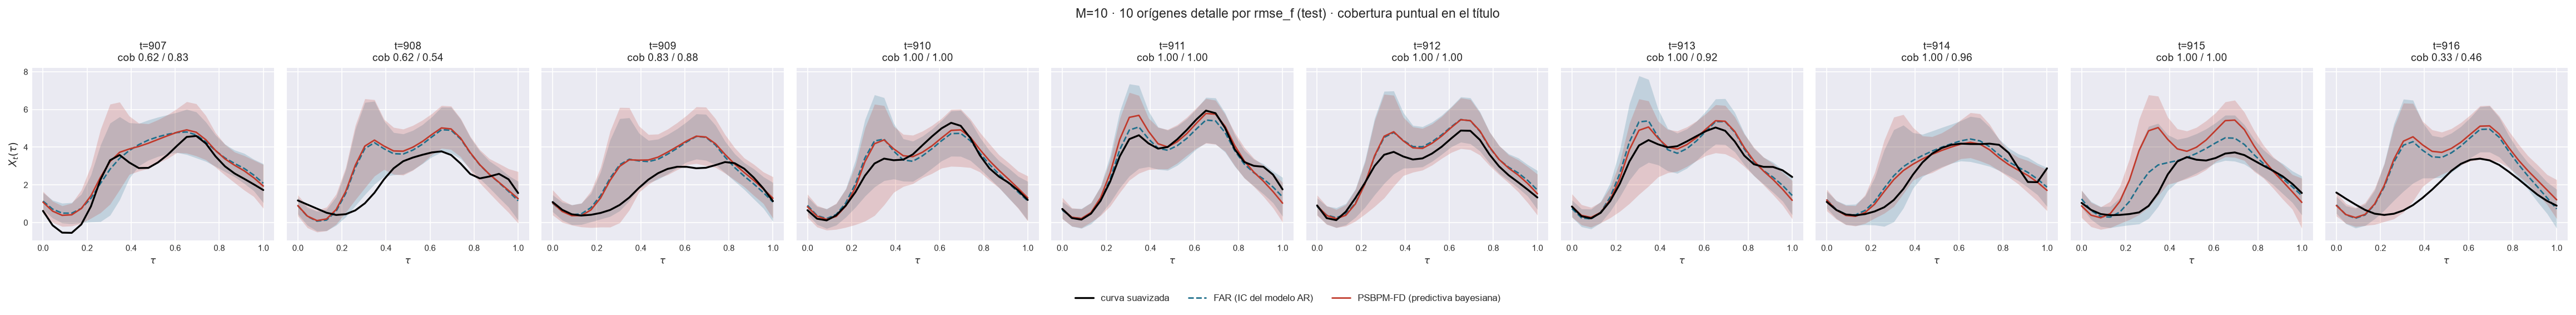
\includegraphics[width=\textwidth,height=0.75\textheight,keepaspectratio]{IMG/aneC_00/aneC_00_79_ic_contraste_detalle_101.png}
\caption{Bandas equi-colas y del FAR en la ventana de detalle, tráfico con rezago $\{1\}$ ($M = 10$).}
\label{fig:aneC_79_ic_contraste_detalle_101}
\end{figure}

\begin{figure}[H]
\centering
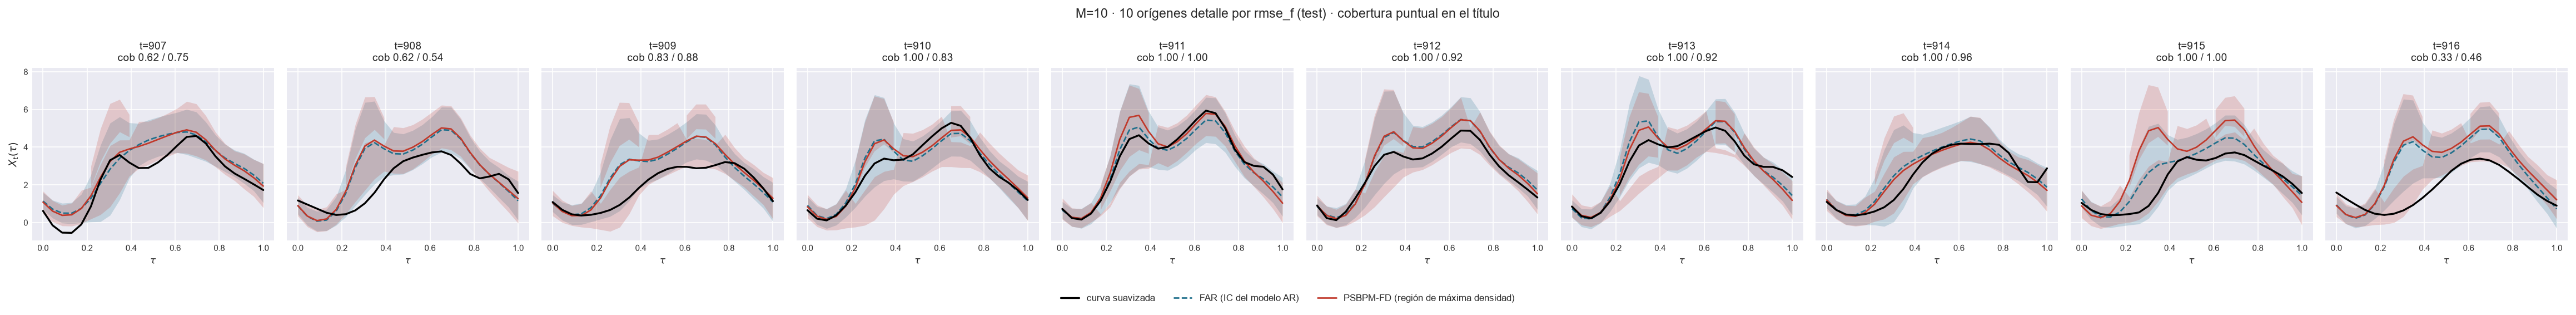
\includegraphics[width=\textwidth,height=0.75\textheight,keepaspectratio]{IMG/aneC_00/aneC_00_79_ic_contraste_detalle_hdr_101.png}
\caption{Región de máxima densidad en la ventana de detalle, tráfico con rezago $\{1\}$ ($M = 10$).}
\label{fig:aneC_79_ic_contraste_detalle_hdr_101}
\end{figure}

\begin{figure}[H]
\centering
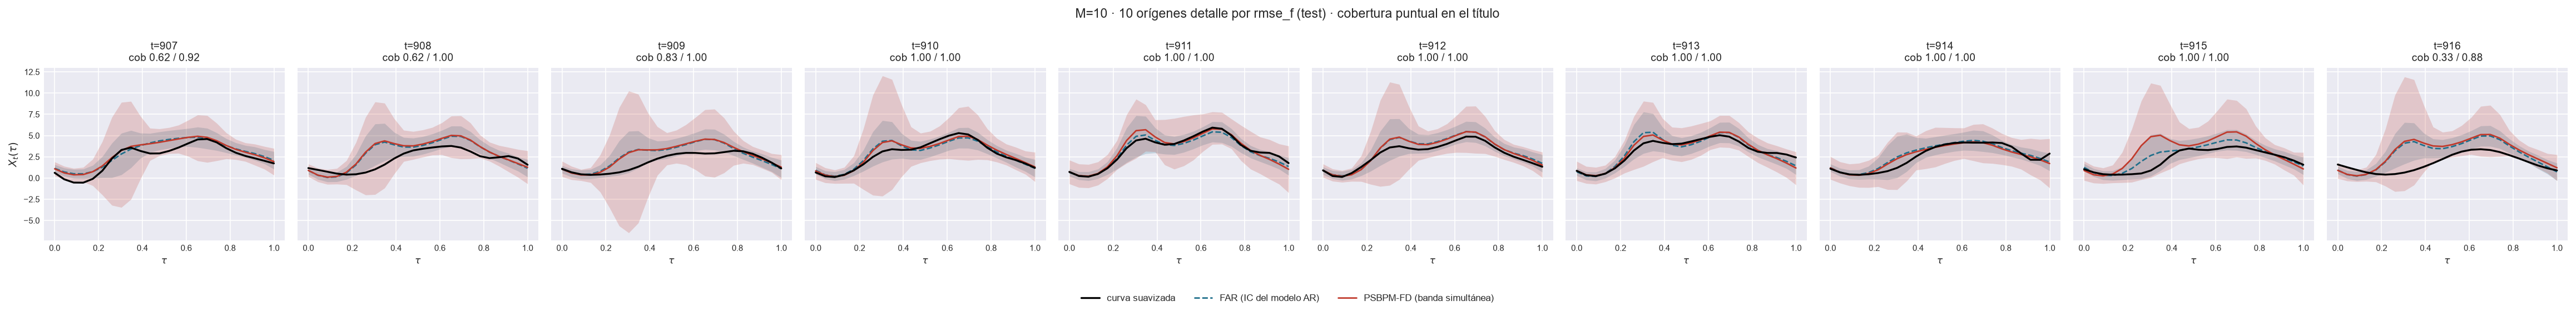
\includegraphics[width=\textwidth,height=0.75\textheight,keepaspectratio]{IMG/aneC_00/aneC_00_79_ic_contraste_detalle_simultanea_101.png}
\caption{Banda simultánea en la ventana de detalle, tráfico con rezago $\{1\}$ ($M = 10$).}
\label{fig:aneC_79_ic_contraste_detalle_simultanea_101}
\end{figure}

\begin{figure}[H]
\centering
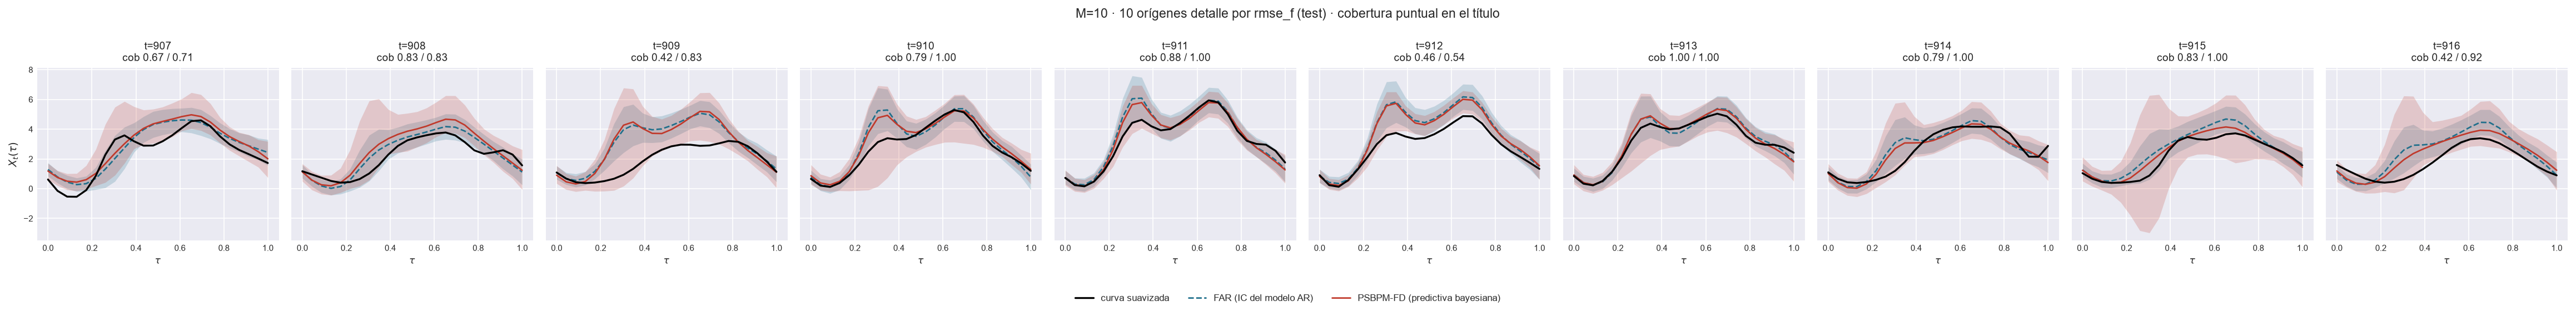
\includegraphics[width=\textwidth,height=0.75\textheight,keepaspectratio]{IMG/aneC_00/aneC_00_79_ic_contraste_detalle_102.png}
\caption{Bandas equi-colas y del FAR en la ventana de detalle, tráfico con rezagos $\{1,7\}$ ($M = 10$).}
\label{fig:aneC_79_ic_contraste_detalle_102}
\end{figure}

\begin{figure}[H]
\centering
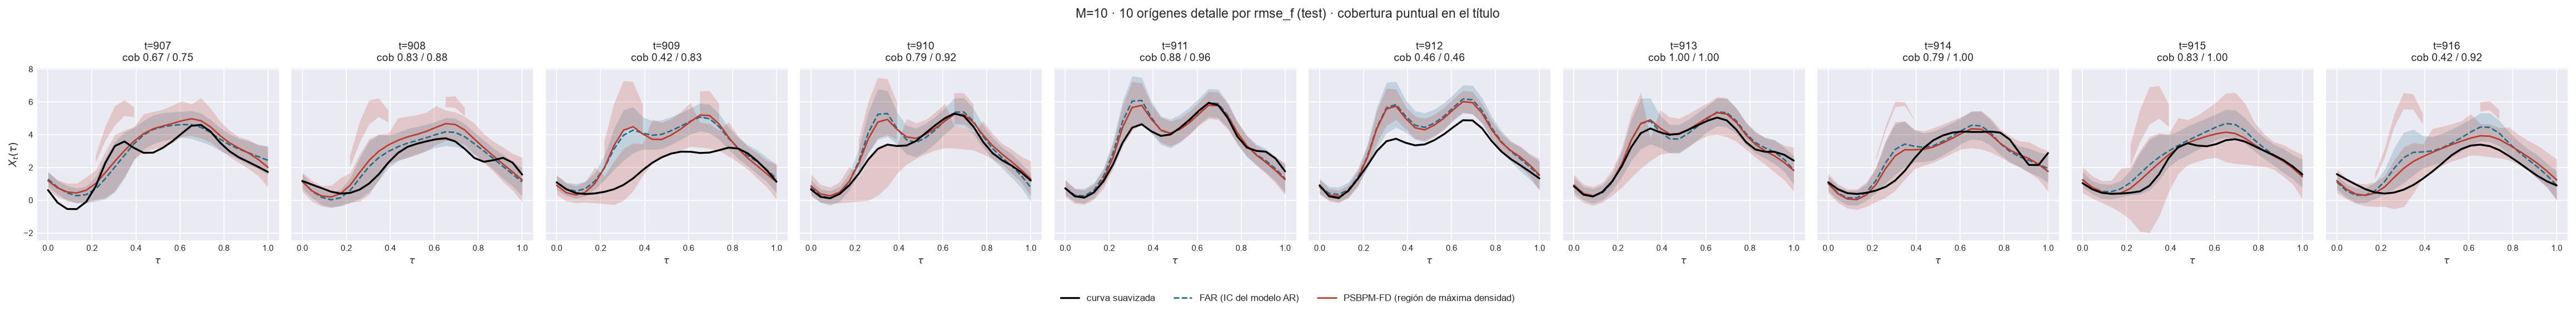
\includegraphics[width=\textwidth,height=0.75\textheight,keepaspectratio]{IMG/aneC_00/aneC_00_79_ic_contraste_detalle_hdr_102.png}
\caption{Región de máxima densidad en la ventana de detalle, tráfico con rezagos $\{1,7\}$ ($M = 10$).}
\label{fig:aneC_79_ic_contraste_detalle_hdr_102}
\end{figure}

\begin{figure}[H]
\centering
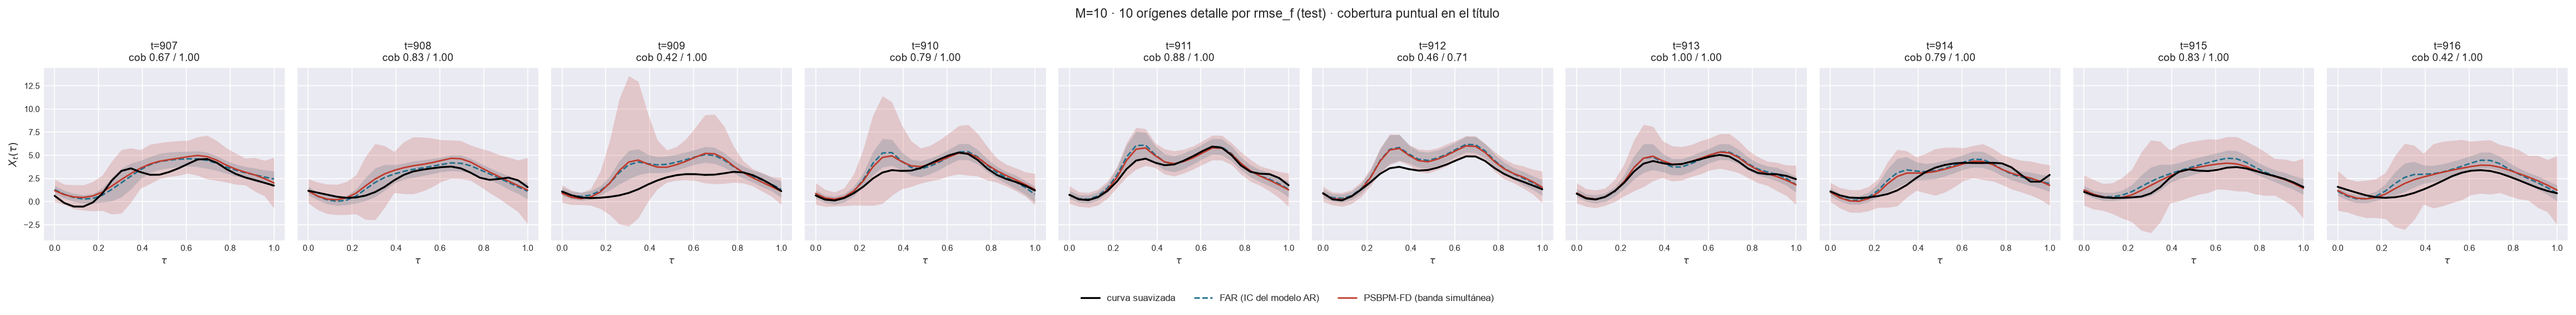
\includegraphics[width=\textwidth,height=0.75\textheight,keepaspectratio]{IMG/aneC_00/aneC_00_79_ic_contraste_detalle_simultanea_102.png}
\caption{Banda simultánea en la ventana de detalle, tráfico con rezagos $\{1,7\}$ ($M = 10$).}
\label{fig:aneC_79_ic_contraste_detalle_simultanea_102}
\end{figure}

\section{Monitoreo por componente}
\label{aneC_00_08_componentes}
% 91-94: error y banda de credibilidad de cada score, como en el Anexo B para simulación.

El error y la banda de credibilidad de cada score, como en la Sección~\ref{aneB_00_05_intervalos_componente} para la simulación.

\begin{figure}[H]
\centering
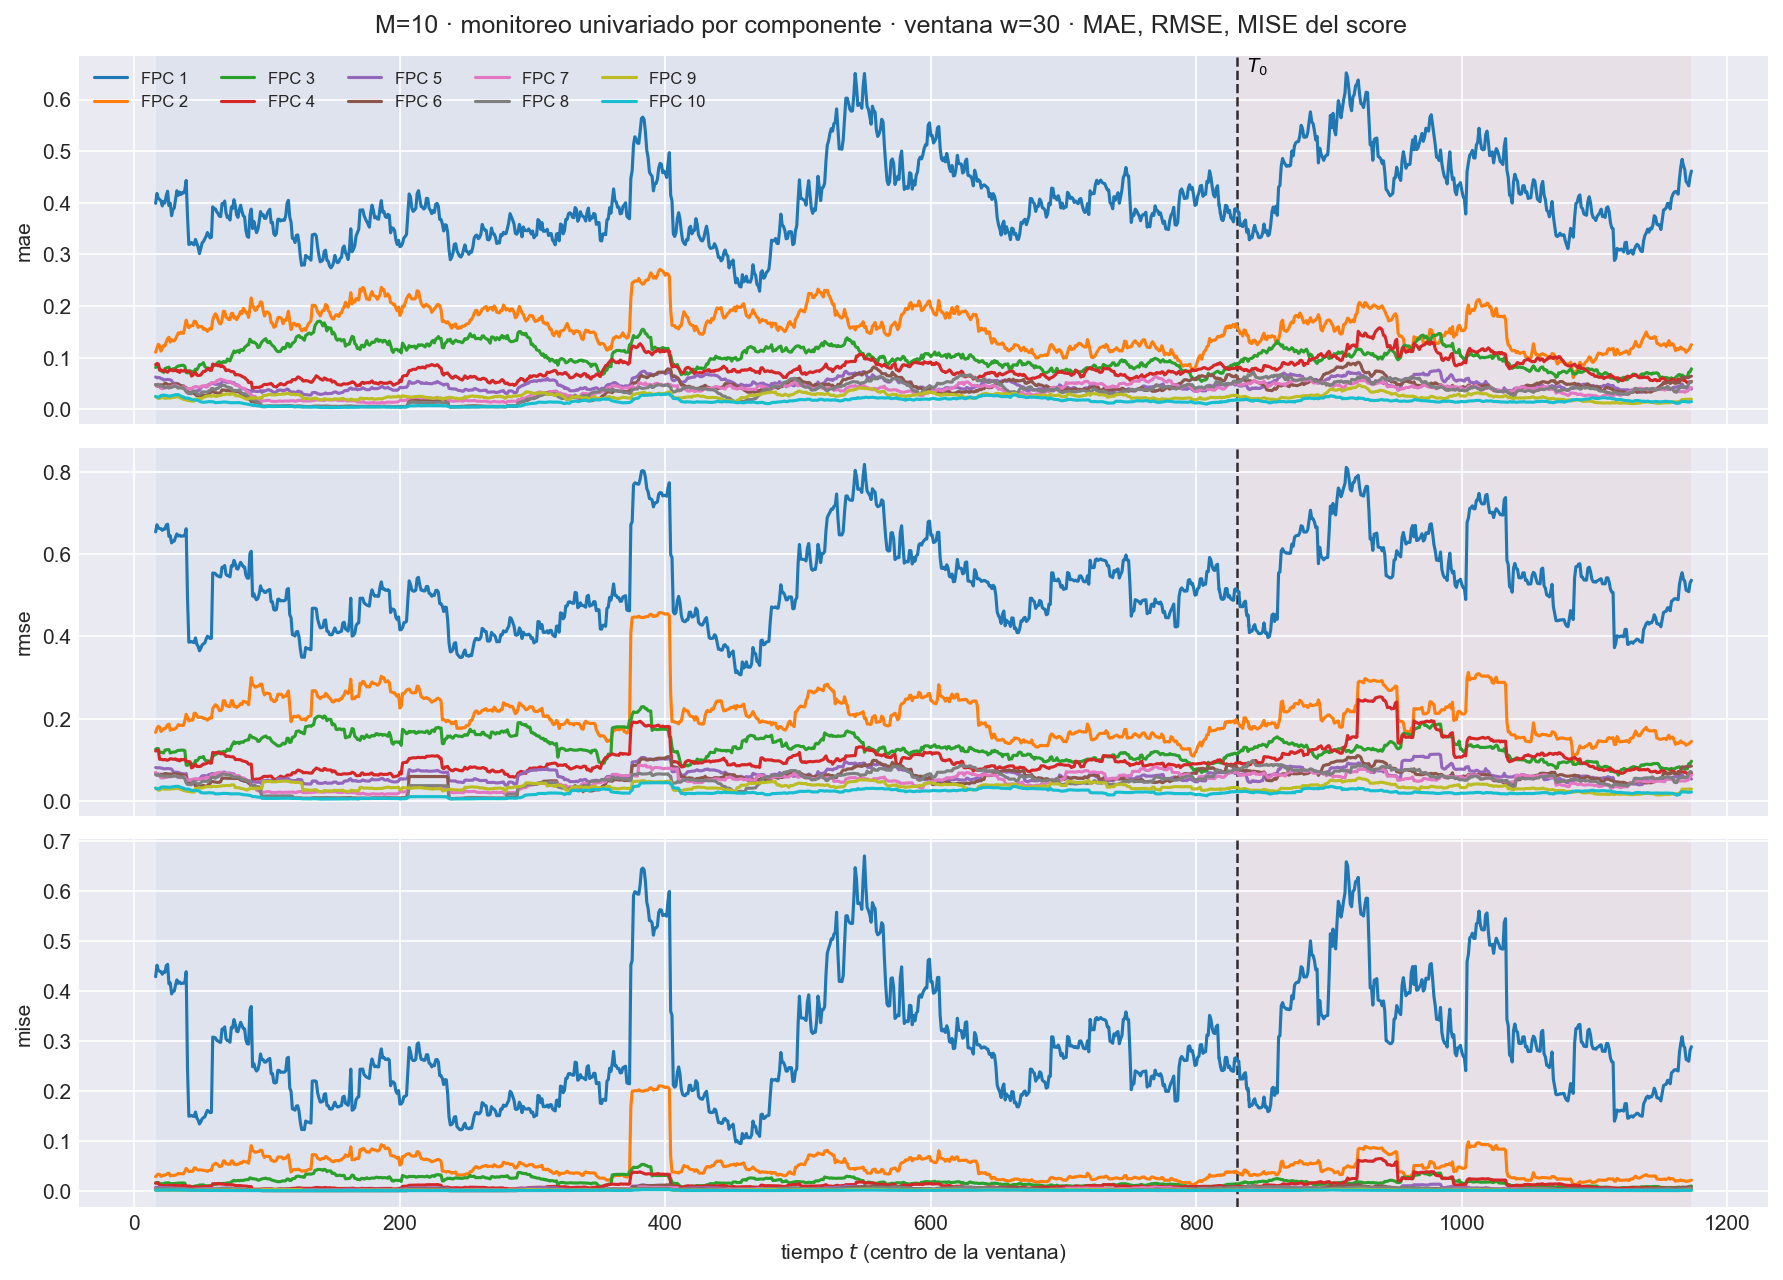
\includegraphics[width=\textwidth,height=0.75\textheight,keepaspectratio]{IMG/aneC_00/aneC_00_91_ventana_univariado_w30_101.png}
\caption{Error de cada score sobre la ventana móvil, tráfico con rezago $\{1\}$ ($M = 10$).}
\label{fig:aneC_91_ventana_univariado_w30_101}
\end{figure}

\begin{figure}[H]
\centering
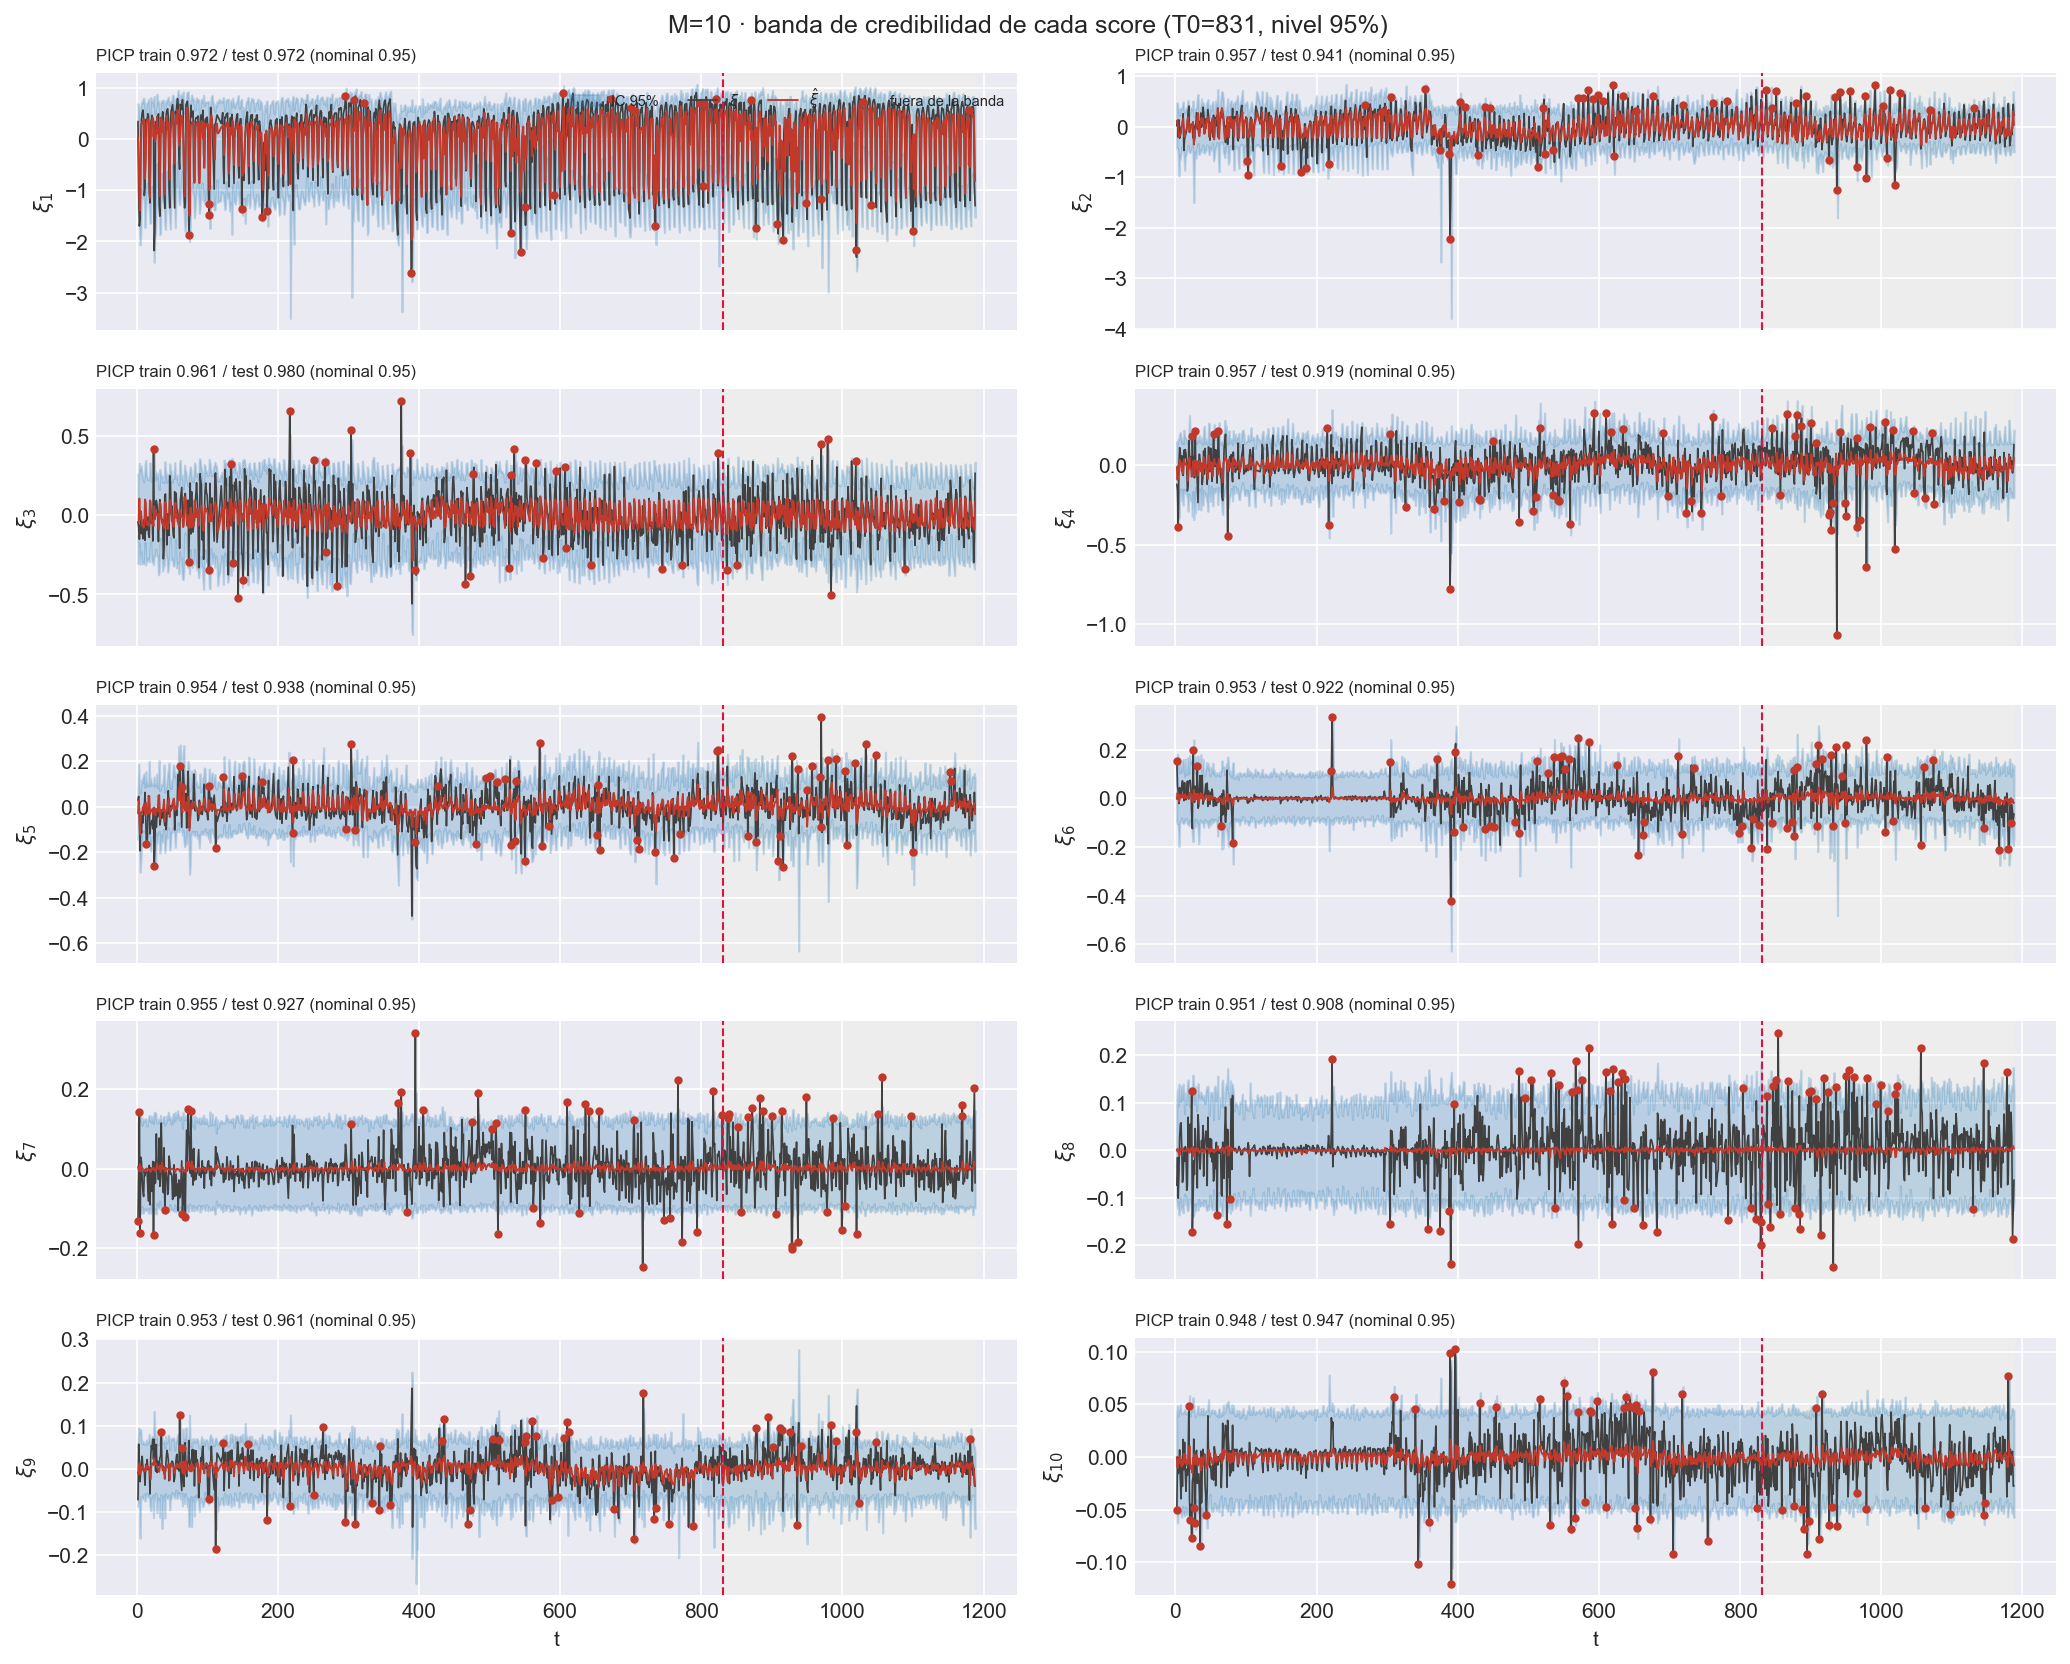
\includegraphics[width=\textwidth,height=0.75\textheight,keepaspectratio]{IMG/aneC_00/aneC_00_92_scores_banda_credibilidad_101.png}
\caption{Banda de credibilidad al 95\% de cada score, tráfico con rezago $\{1\}$ ($M = 10$).}
\label{fig:aneC_92_scores_banda_credibilidad_101}
\end{figure}

\begin{figure}[H]
\centering
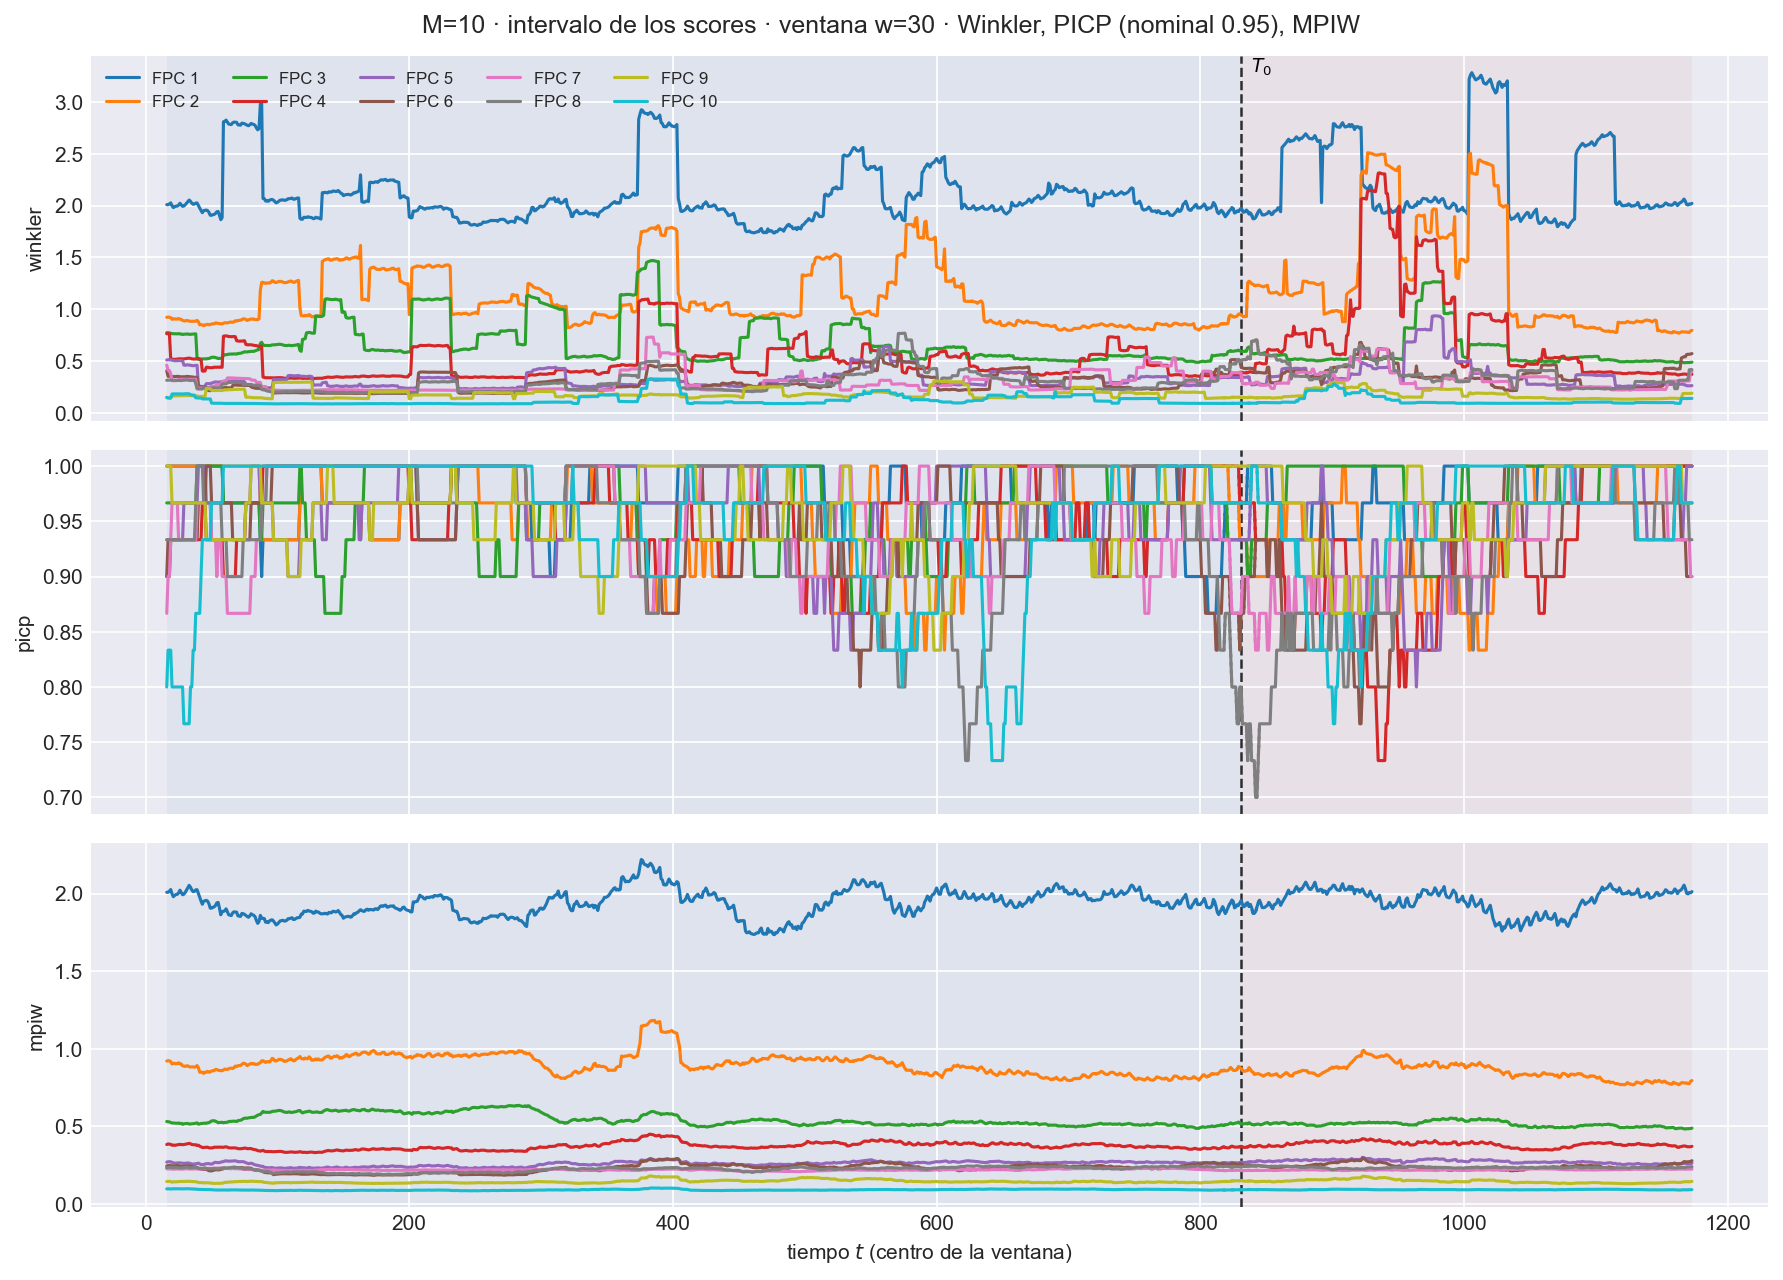
\includegraphics[width=\textwidth,height=0.75\textheight,keepaspectratio]{IMG/aneC_00/aneC_00_93_ventana_scores_intervalo_w30_101.png}
\caption{Métricas de intervalo de cada score sobre la ventana móvil, tráfico con rezago $\{1\}$ ($M = 10$).}
\label{fig:aneC_93_ventana_scores_intervalo_w30_101}
\end{figure}

\begin{figure}[H]
\centering
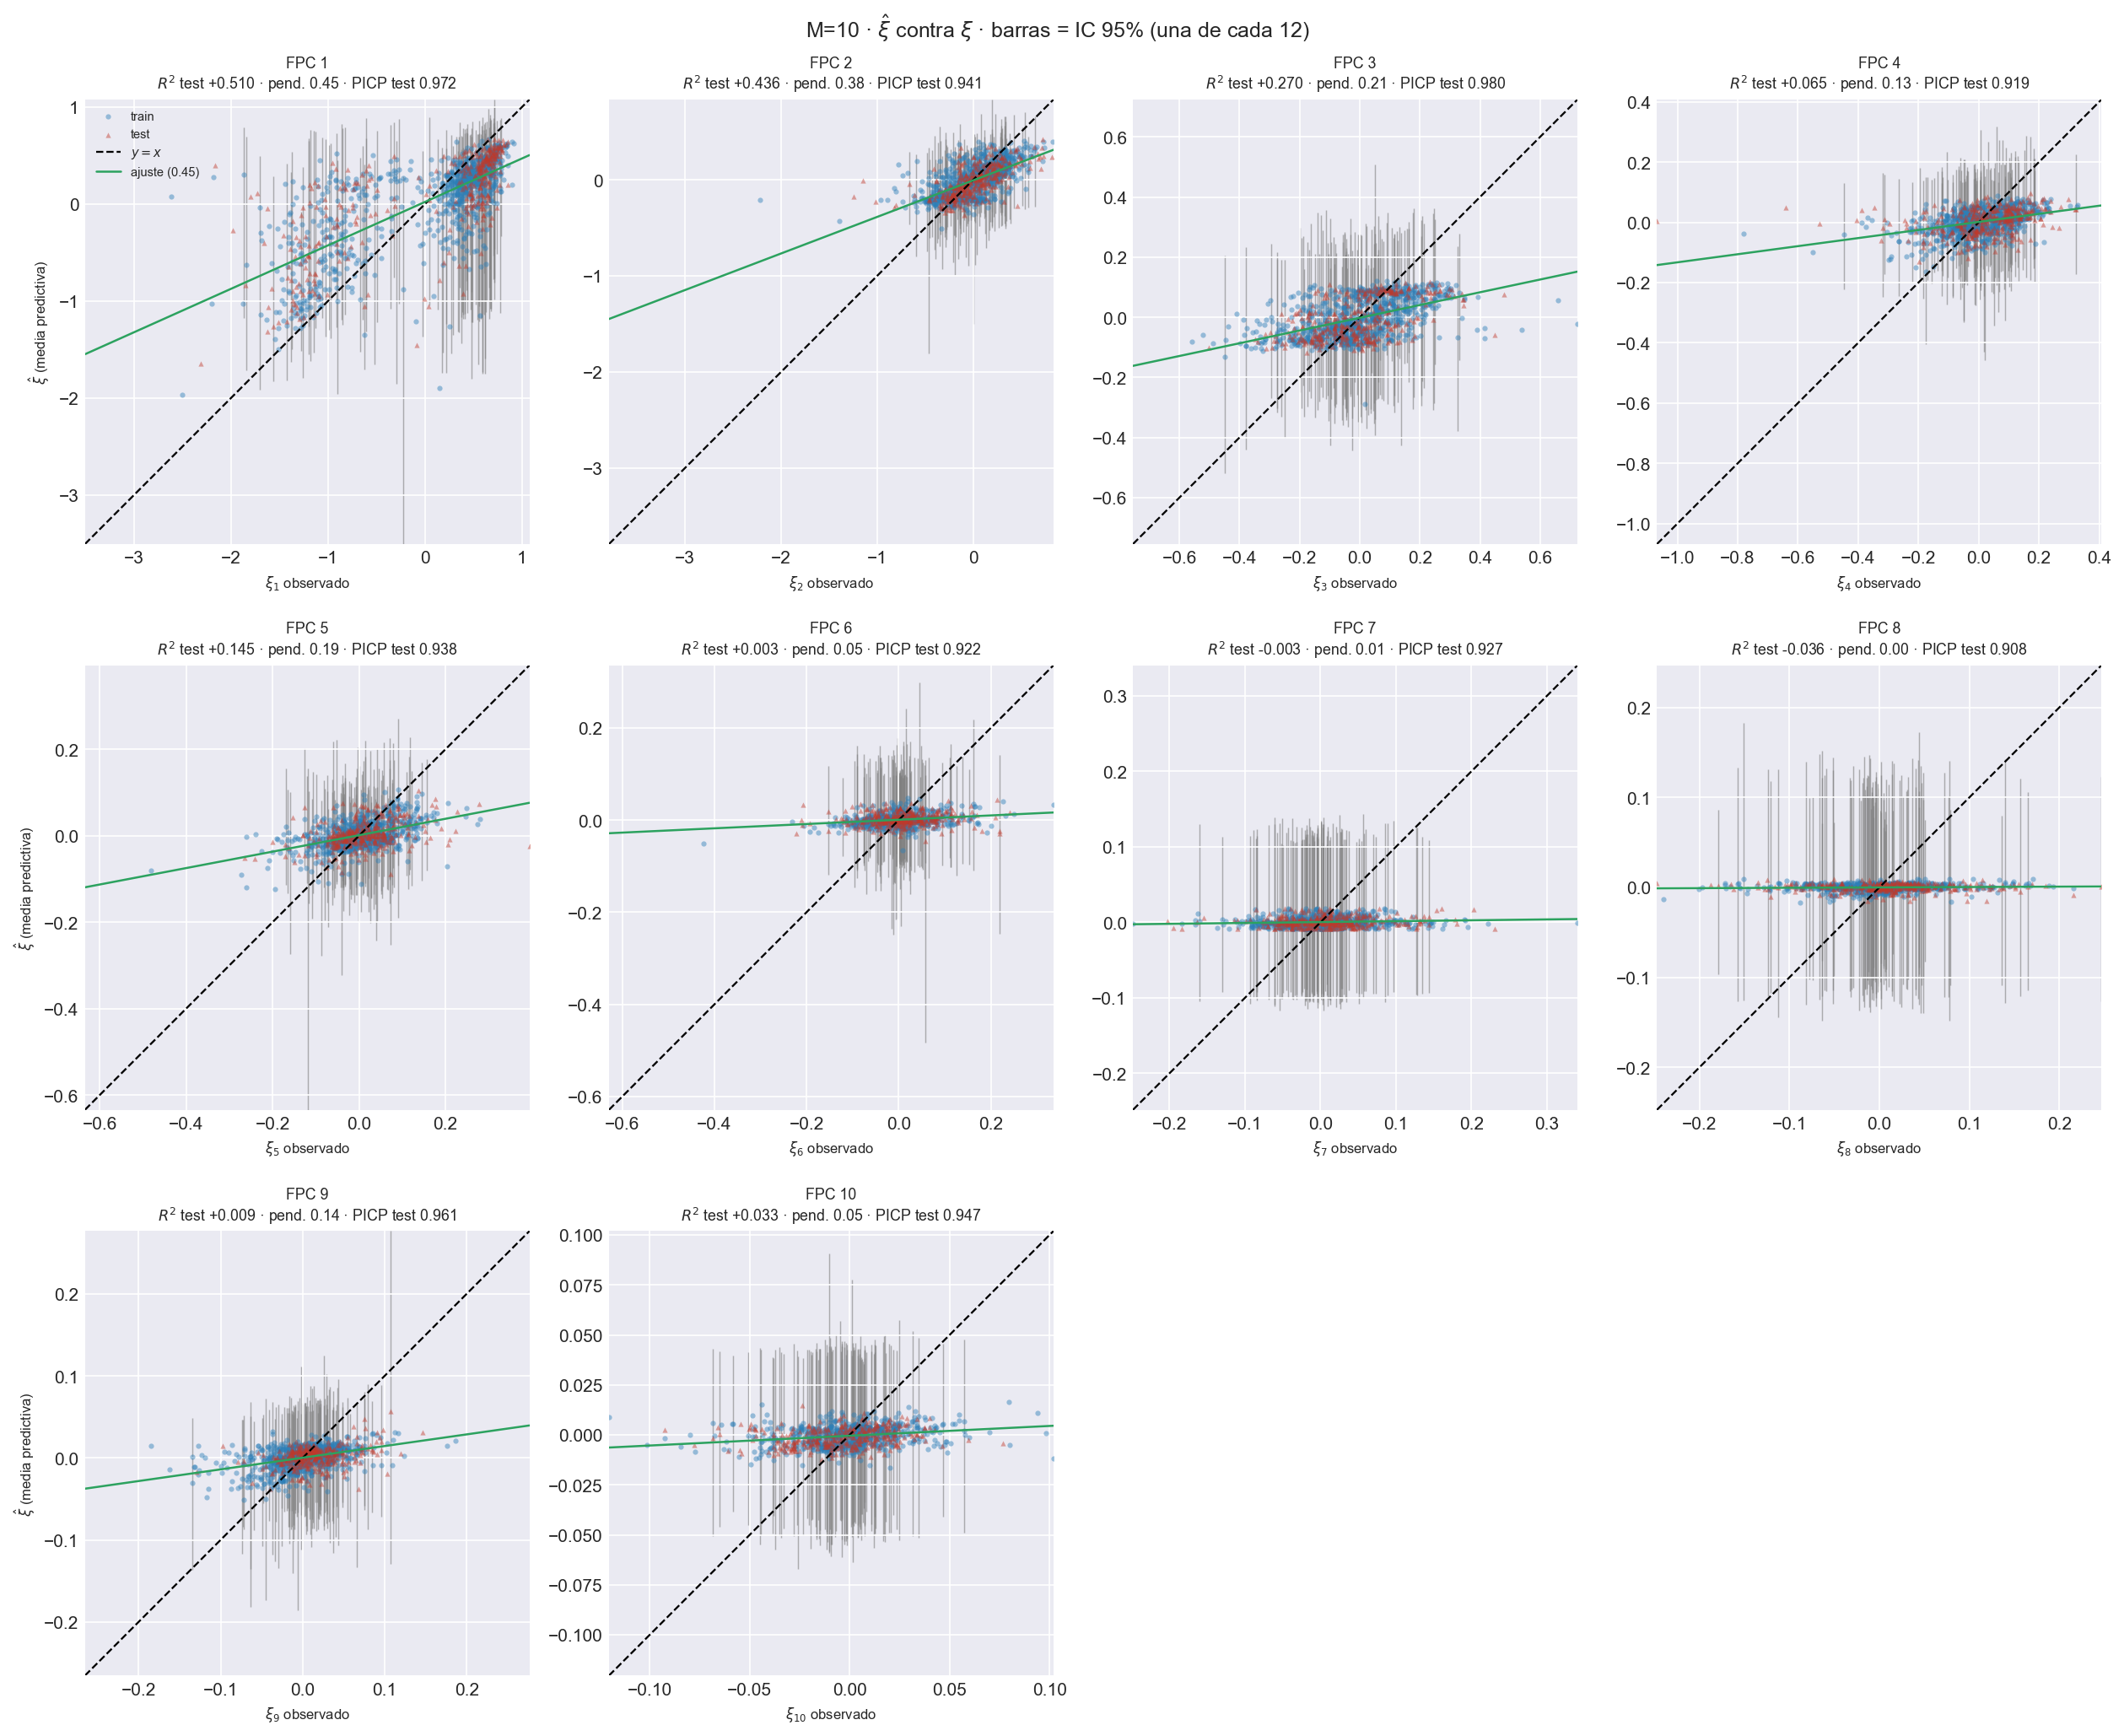
\includegraphics[width=\textwidth,height=0.75\textheight,keepaspectratio]{IMG/aneC_00/aneC_00_94_scores_dispersion_vs_real_101.png}
\caption{Dispersión estimada de cada score frente a la observada, tráfico con rezago $\{1\}$ ($M = 10$).}
\label{fig:aneC_94_scores_dispersion_vs_real_101}
\end{figure}

\begin{figure}[H]
\centering
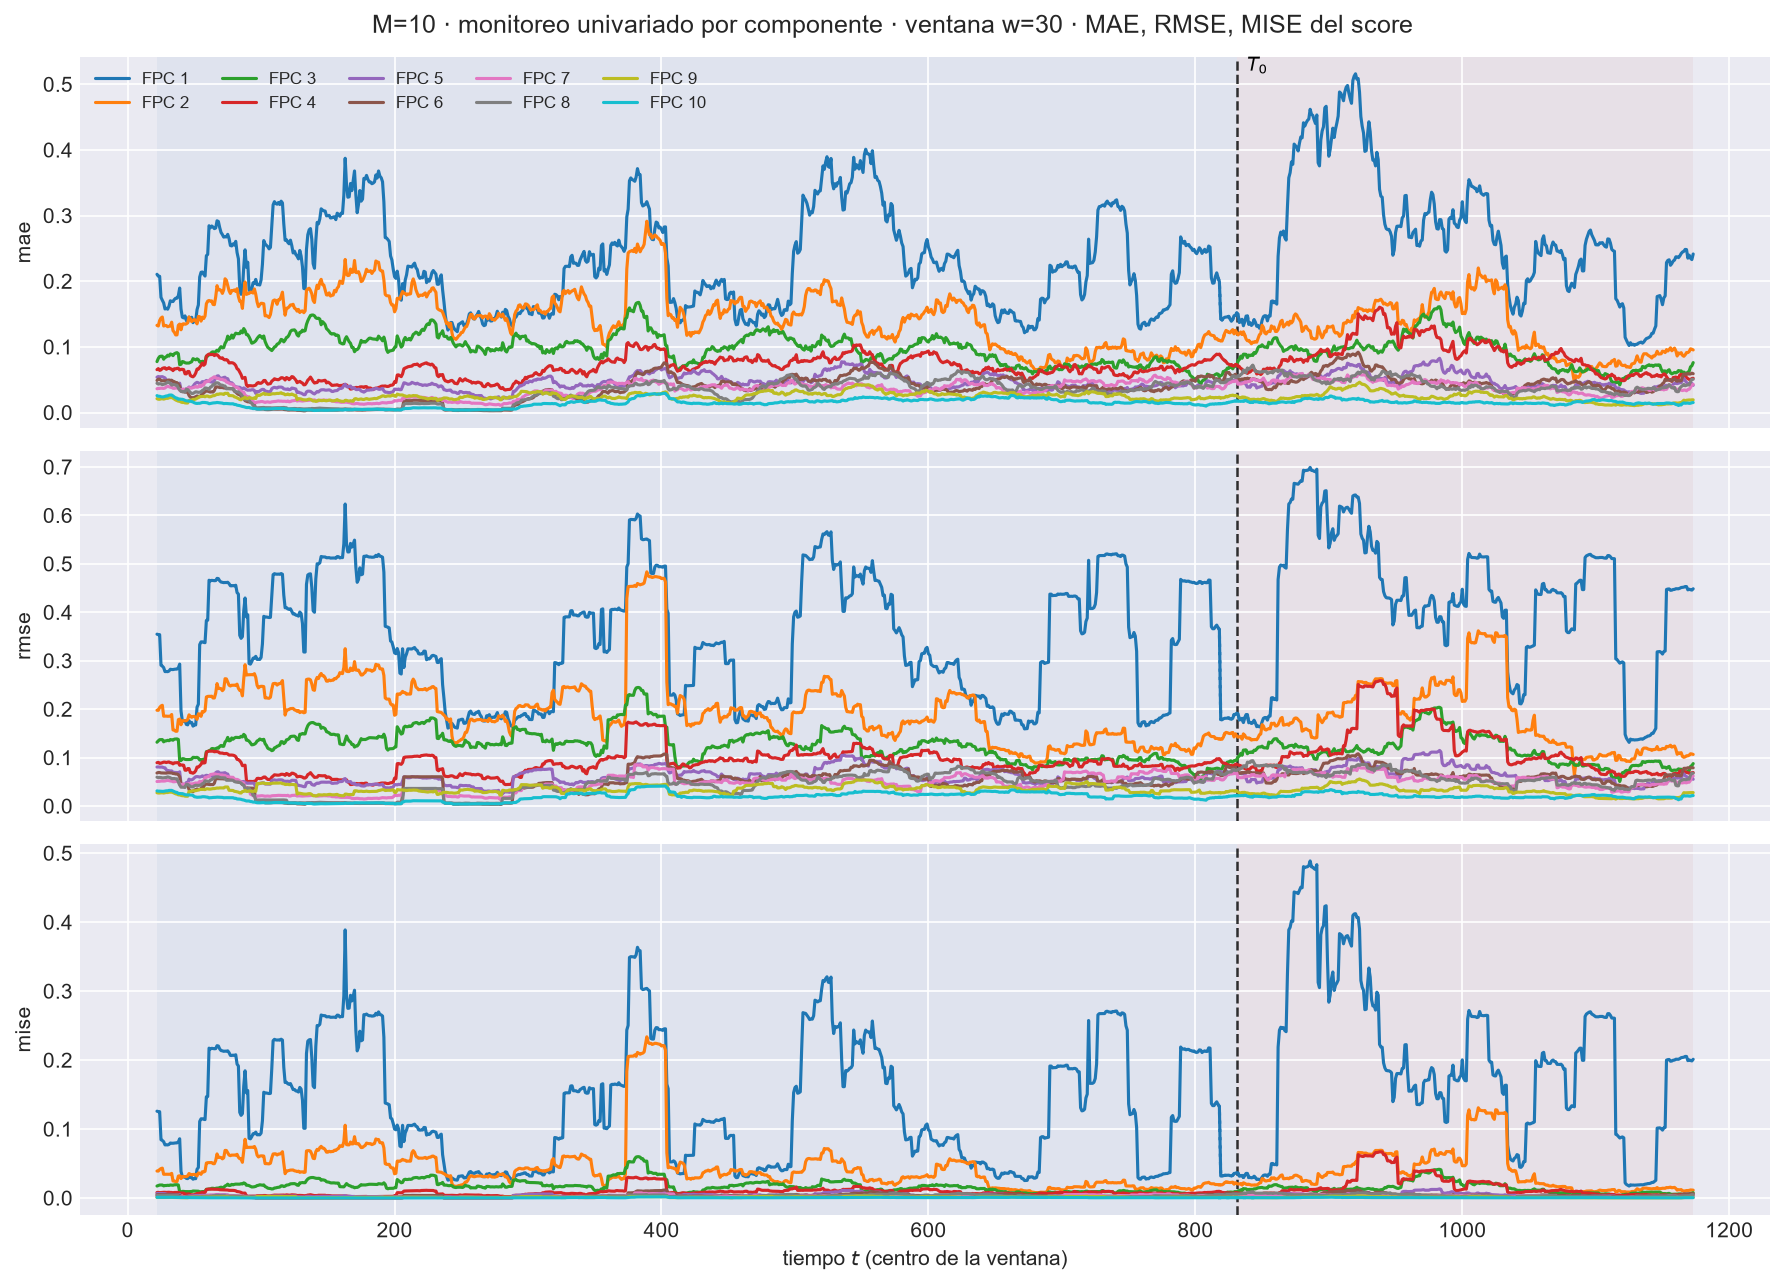
\includegraphics[width=\textwidth,height=0.75\textheight,keepaspectratio]{IMG/aneC_00/aneC_00_91_ventana_univariado_w30_102.png}
\caption{Error de cada score sobre la ventana móvil, tráfico con rezagos $\{1,7\}$ ($M = 10$).}
\label{fig:aneC_91_ventana_univariado_w30_102}
\end{figure}

\begin{figure}[H]
\centering
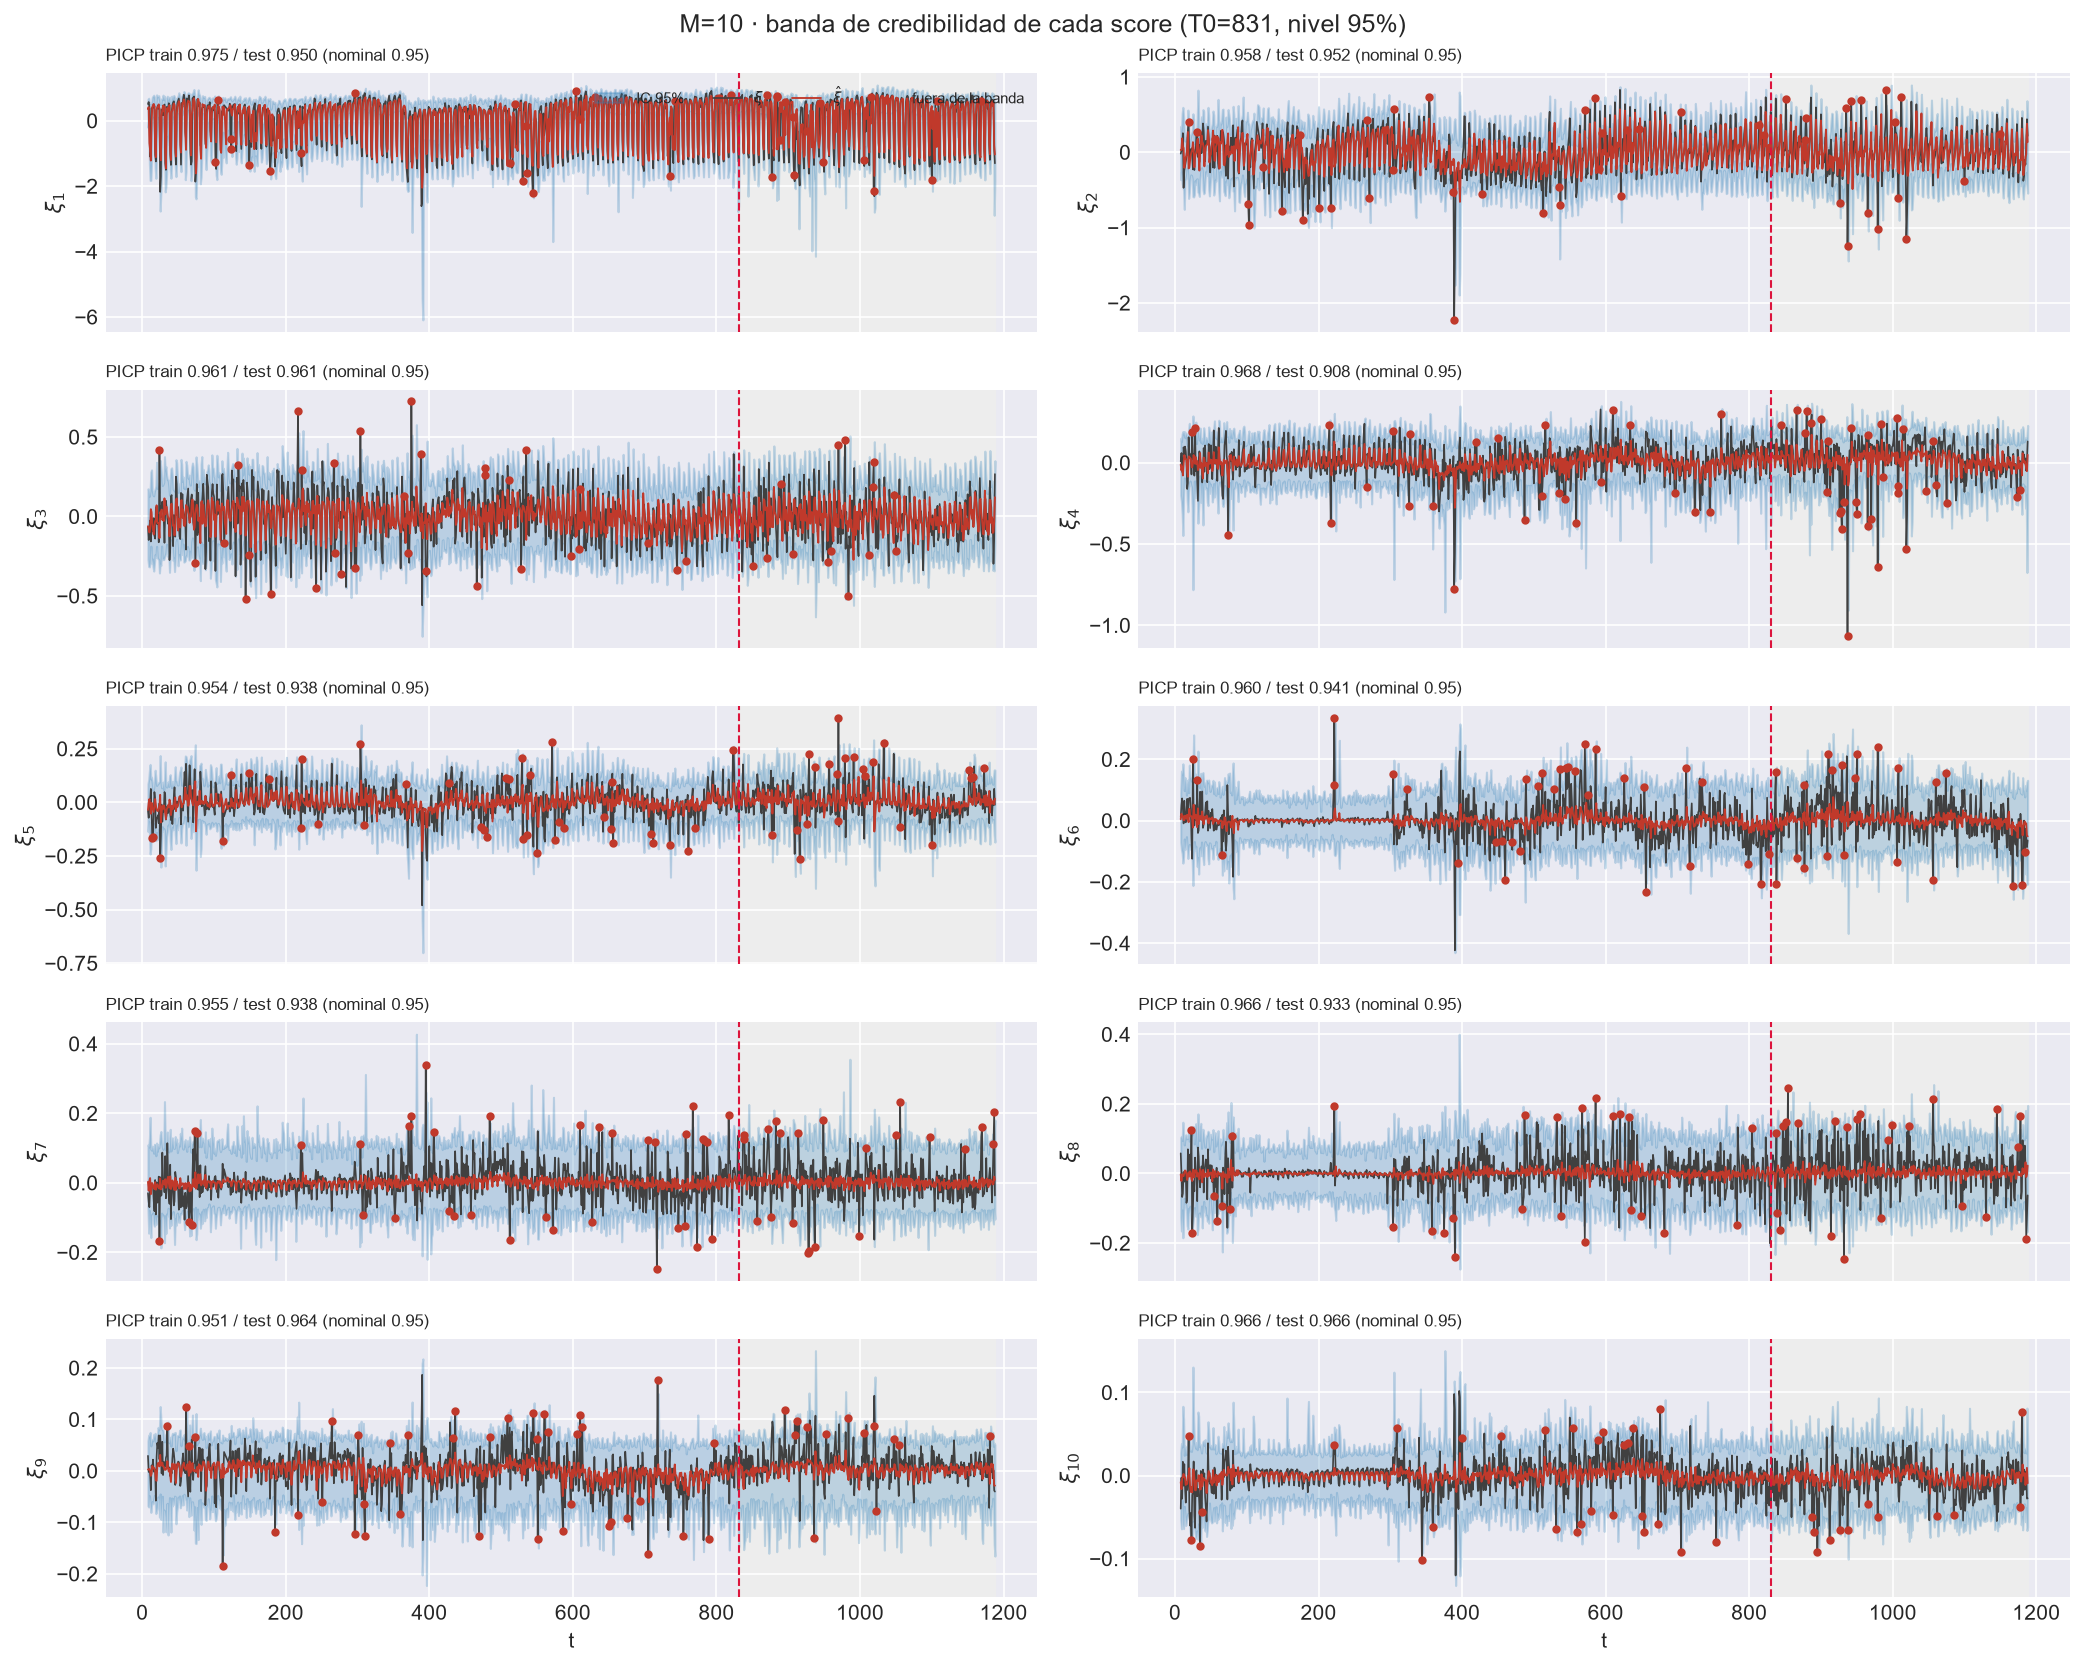
\includegraphics[width=\textwidth,height=0.75\textheight,keepaspectratio]{IMG/aneC_00/aneC_00_92_scores_banda_credibilidad_102.png}
\caption{Banda de credibilidad al 95\% de cada score, tráfico con rezagos $\{1,7\}$ ($M = 10$).}
\label{fig:aneC_92_scores_banda_credibilidad_102}
\end{figure}

\begin{figure}[H]
\centering
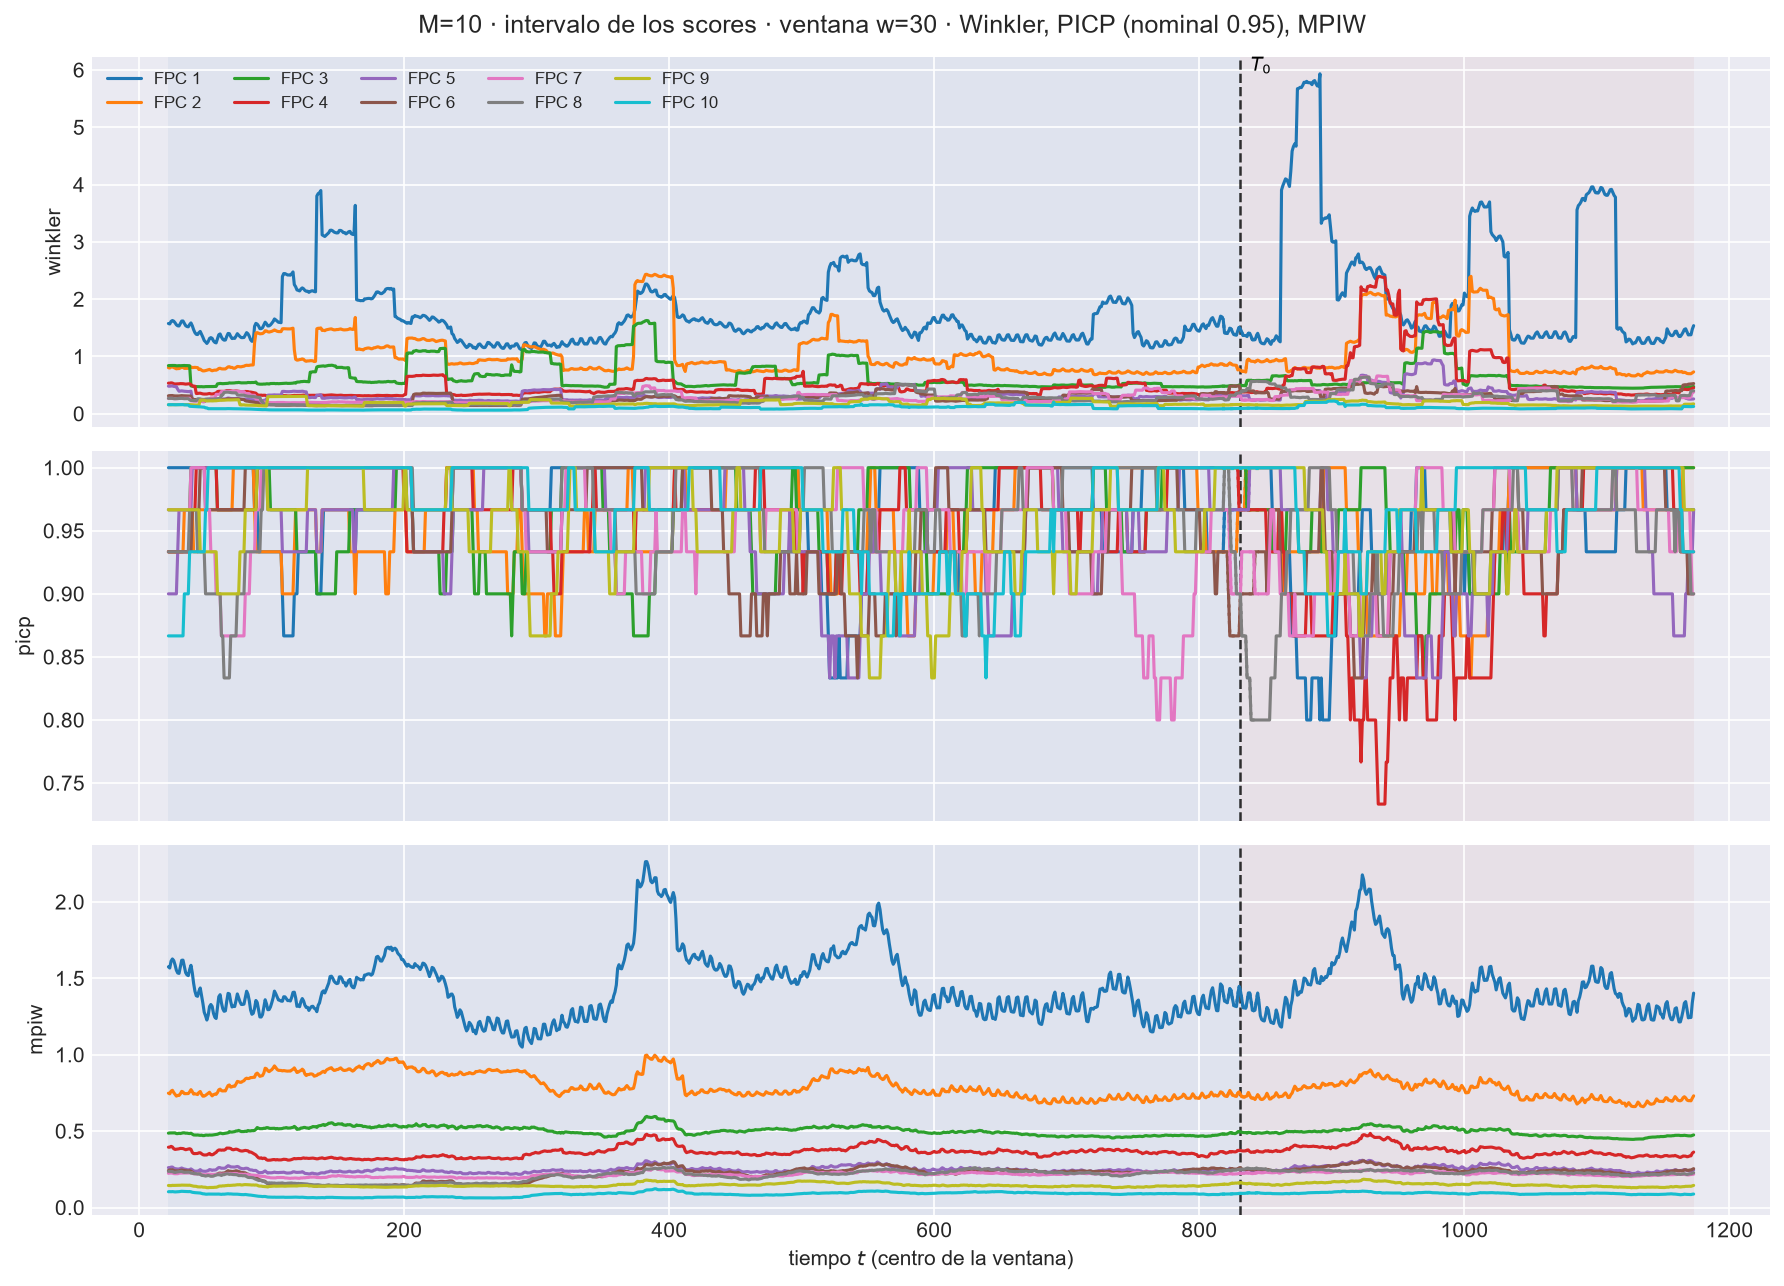
\includegraphics[width=\textwidth,height=0.75\textheight,keepaspectratio]{IMG/aneC_00/aneC_00_93_ventana_scores_intervalo_w30_102.png}
\caption{Métricas de intervalo de cada score sobre la ventana móvil, tráfico con rezagos $\{1,7\}$ ($M = 10$).}
\label{fig:aneC_93_ventana_scores_intervalo_w30_102}
\end{figure}

\begin{figure}[H]
\centering
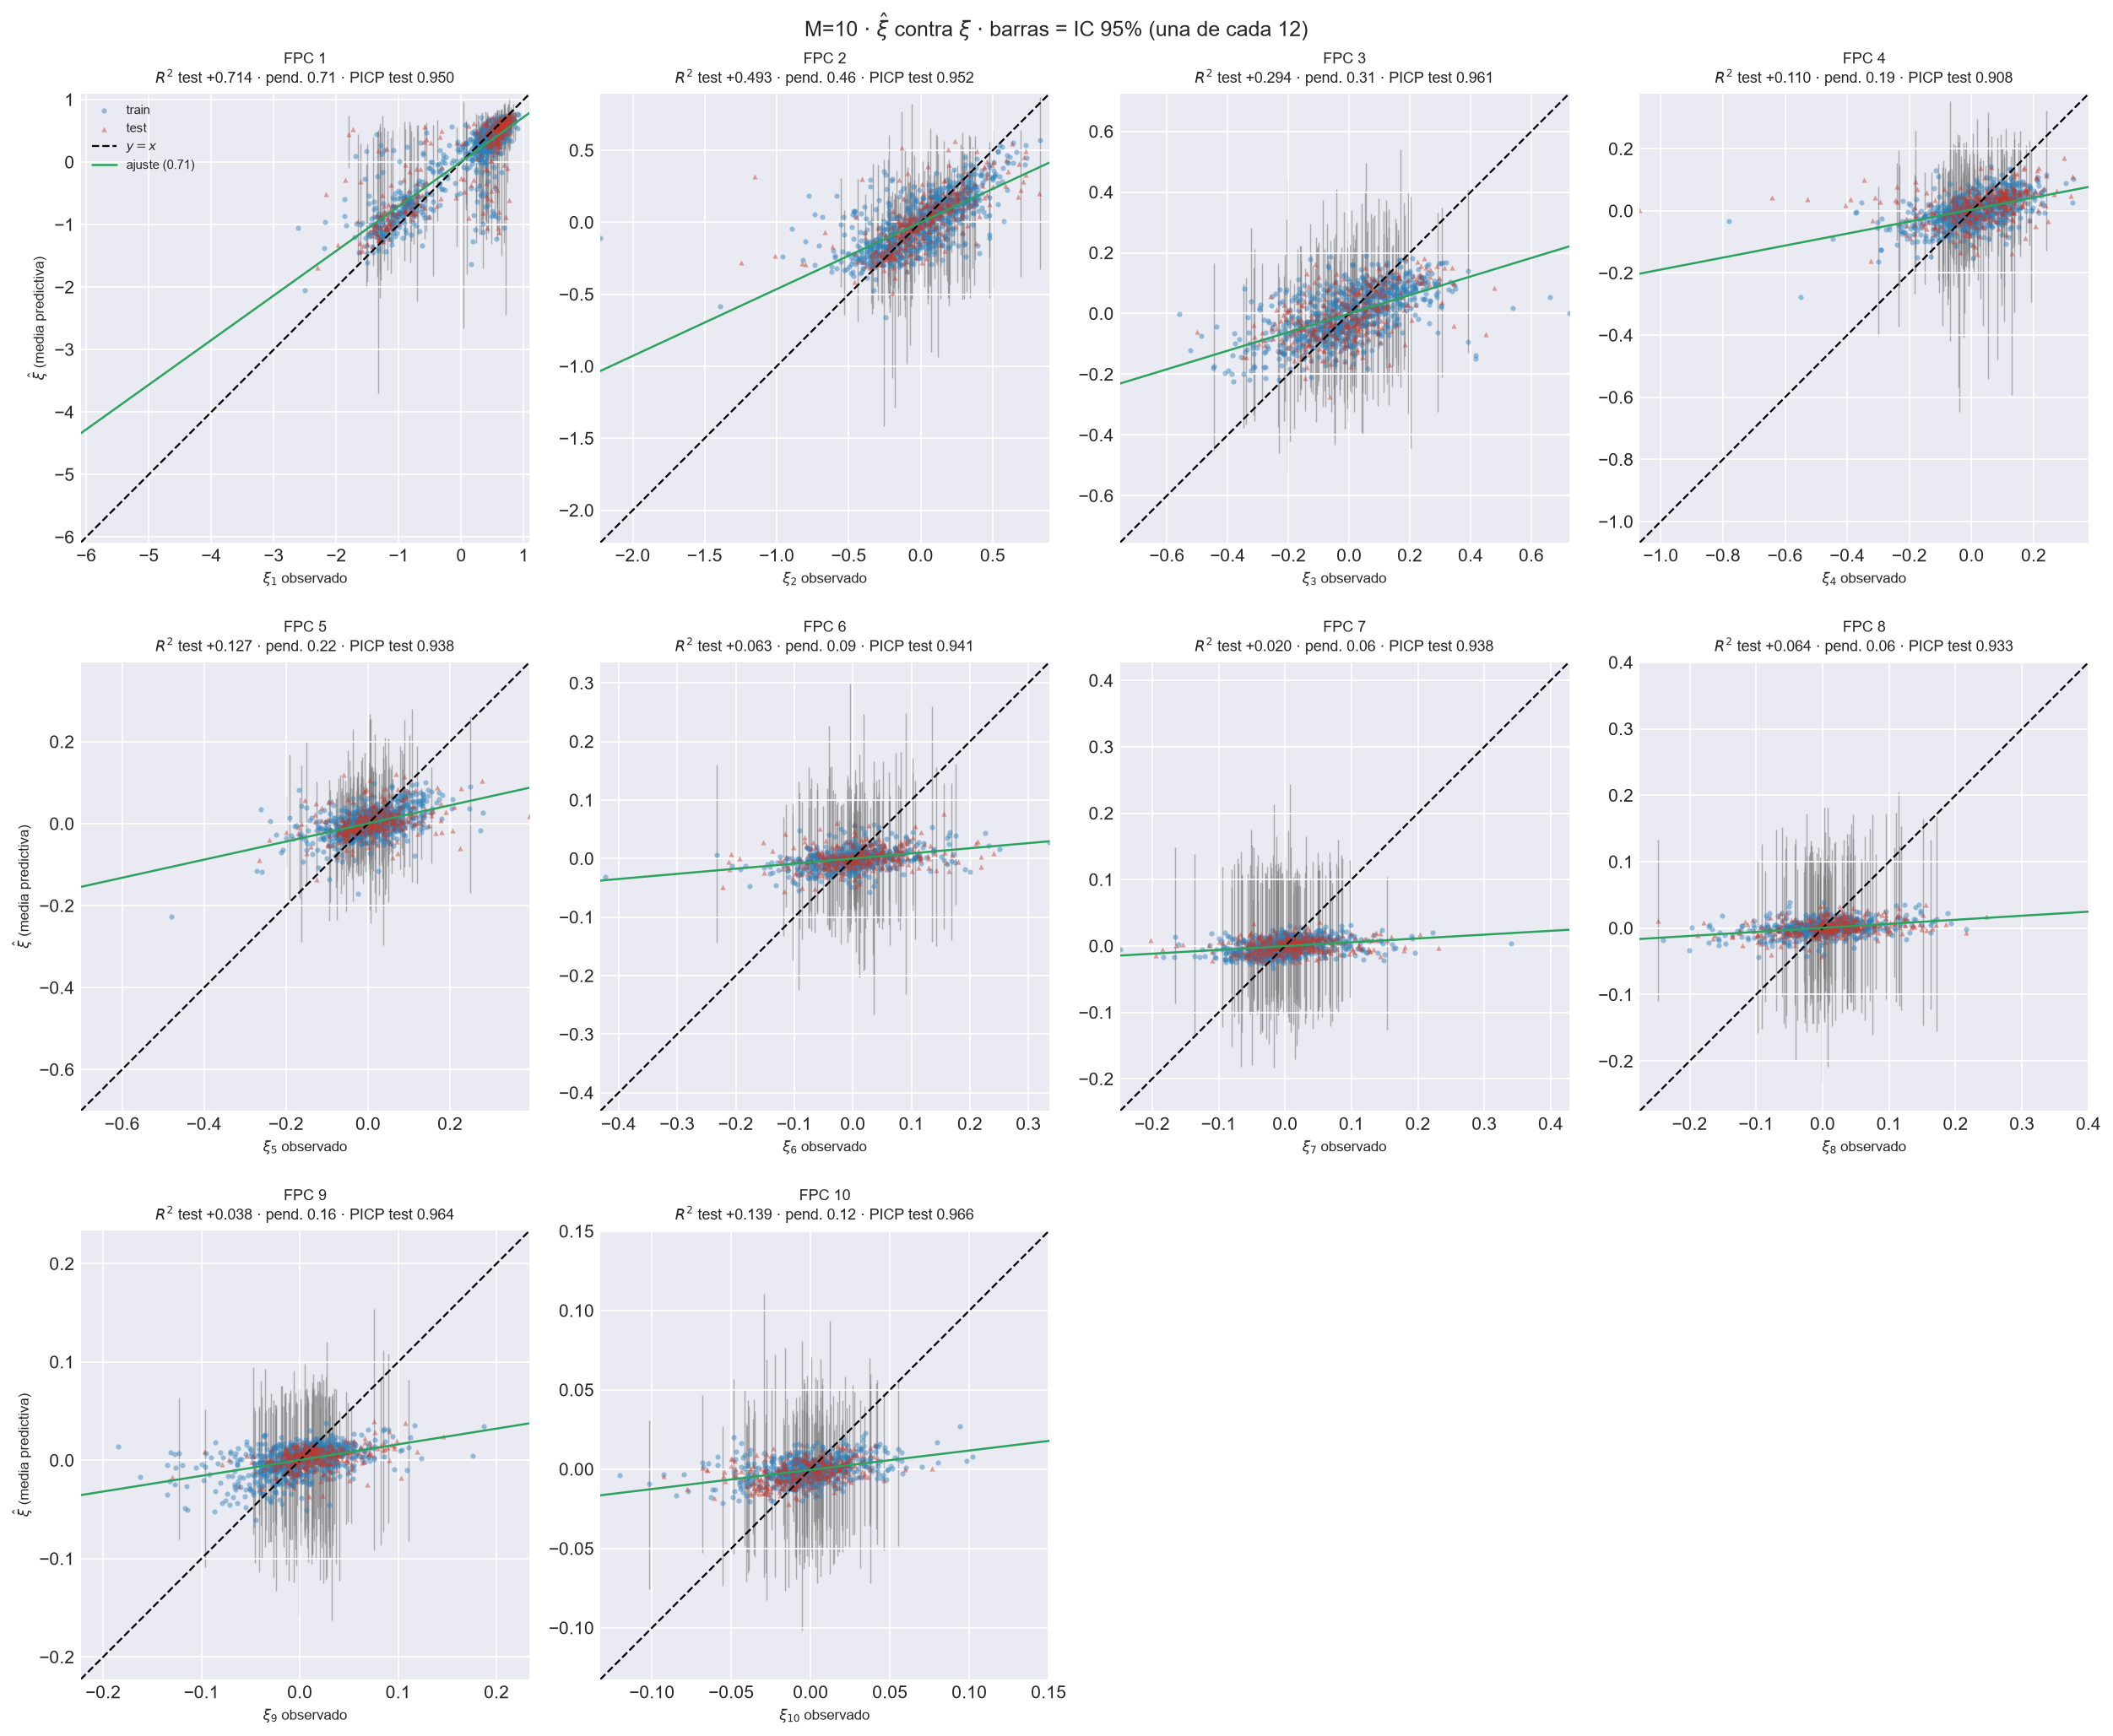
\includegraphics[width=\textwidth,height=0.75\textheight,keepaspectratio]{IMG/aneC_00/aneC_00_94_scores_dispersion_vs_real_102.png}
\caption{Dispersión estimada de cada score frente a la observada, tráfico con rezagos $\{1,7\}$ ($M = 10$).}
\label{fig:aneC_94_scores_dispersion_vs_real_102}
\end{figure}

\section{Selección de variables en los scores menores}
\label{aneC_00_09_seleccion}
% Autofunciones 1-4 y 5-10 (scratchpad figuras_pip.py) y PIP global con burn = 1000 (= 46_pip.csv del _03 de 101 y 102).

Complementa la Sección~\ref{04_03_05_seleccion} con las autofunciones de la FPCA y la ocupación de cada mezcla, que condiciona la lectura de la PIP.

\begin{figure}[H]
\centering
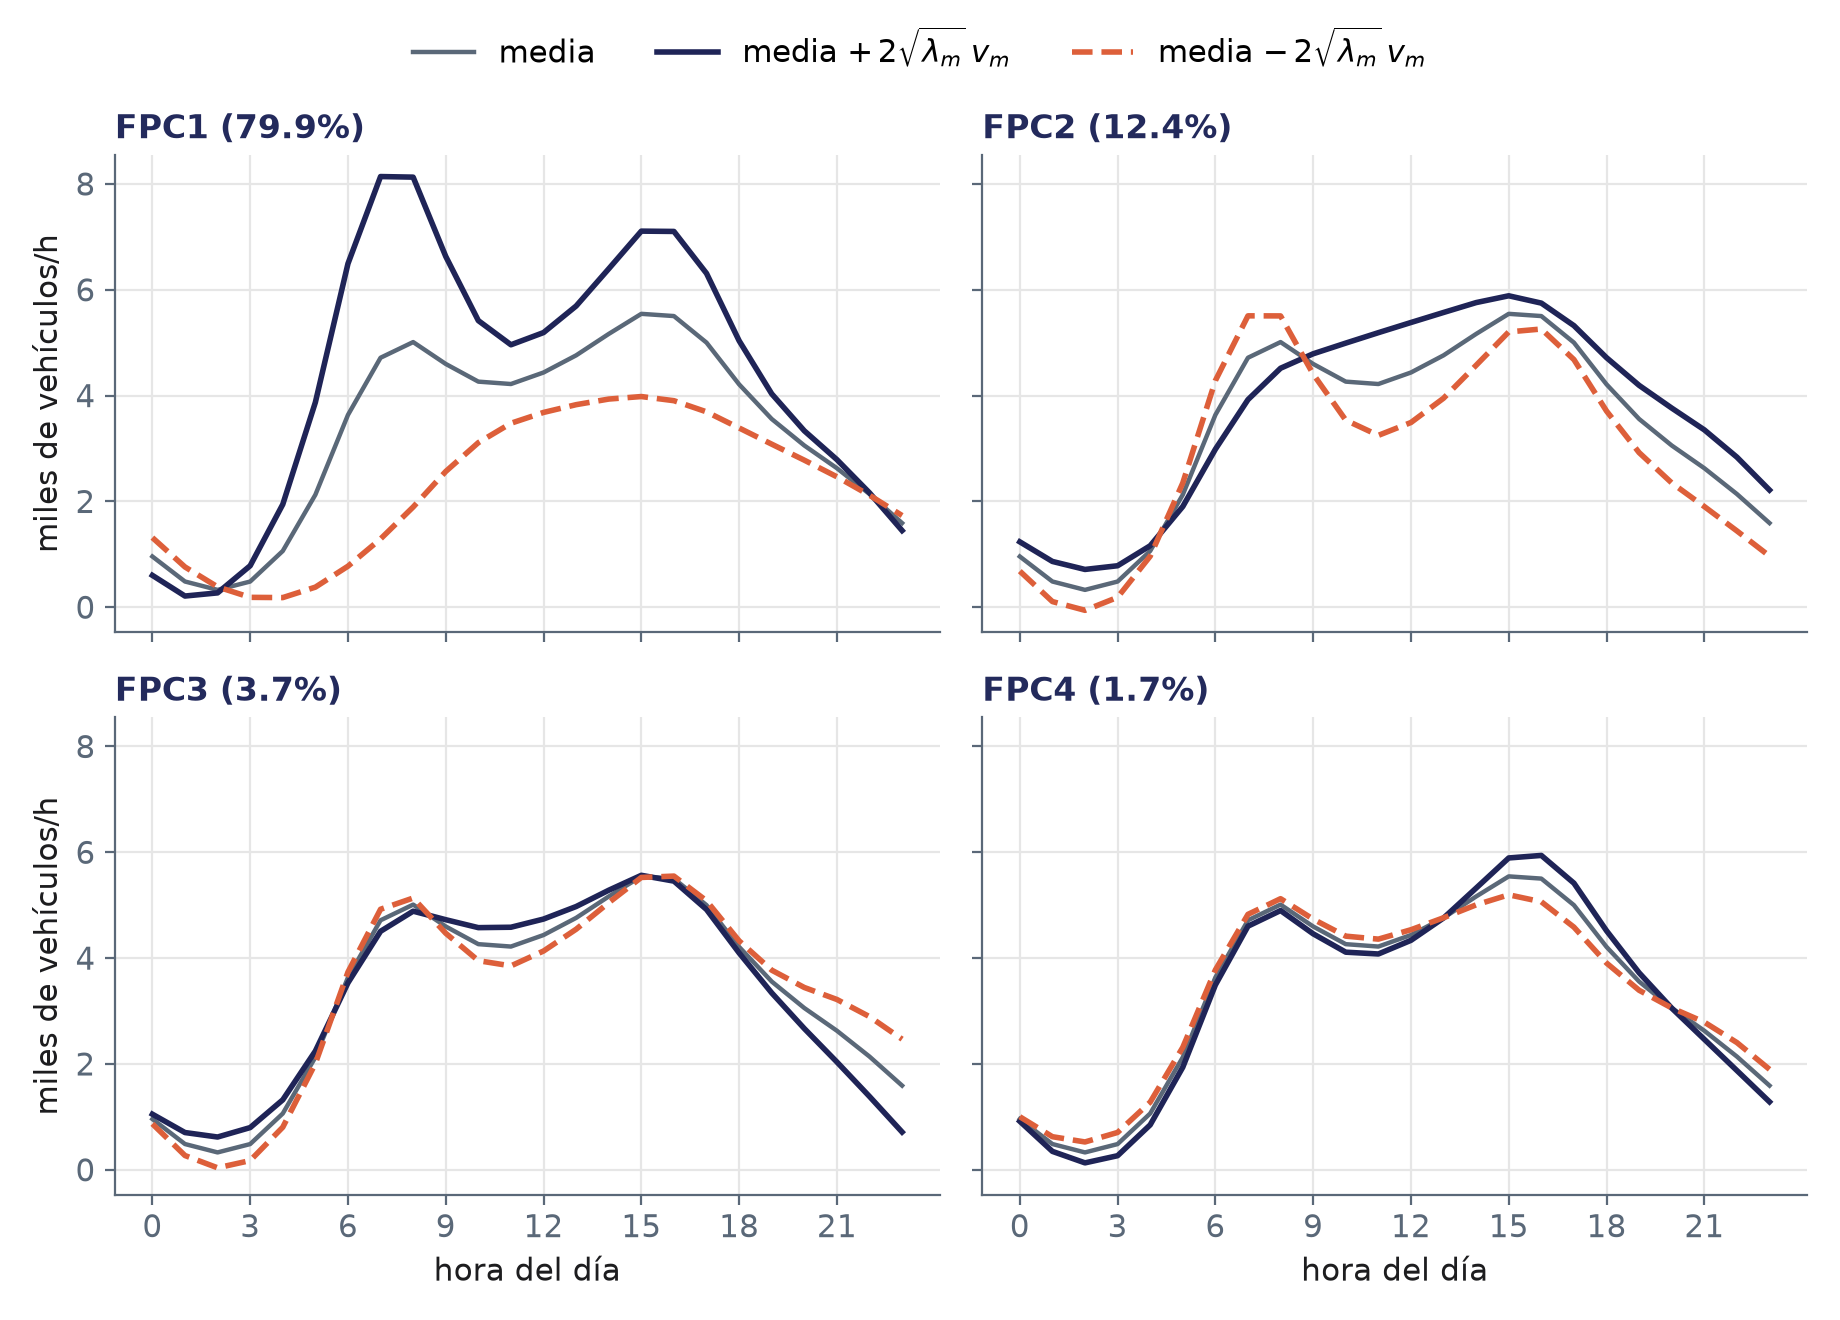
\includegraphics[width=\textwidth,height=0.45\textheight,keepaspectratio]{IMG/aneC_00/aneC_00_autofunciones.png}
\caption{Curva media del bloque de entrenamiento y su perturbación $\mu \pm 2\sqrt{\lambda_m}\,v_m$ a lo largo de las cuatro primeras autofunciones, con la fracción de varianza que explica cada una.}
\label{fig:aneC_autofunciones}
\end{figure}

\begin{figure}[H]
\centering
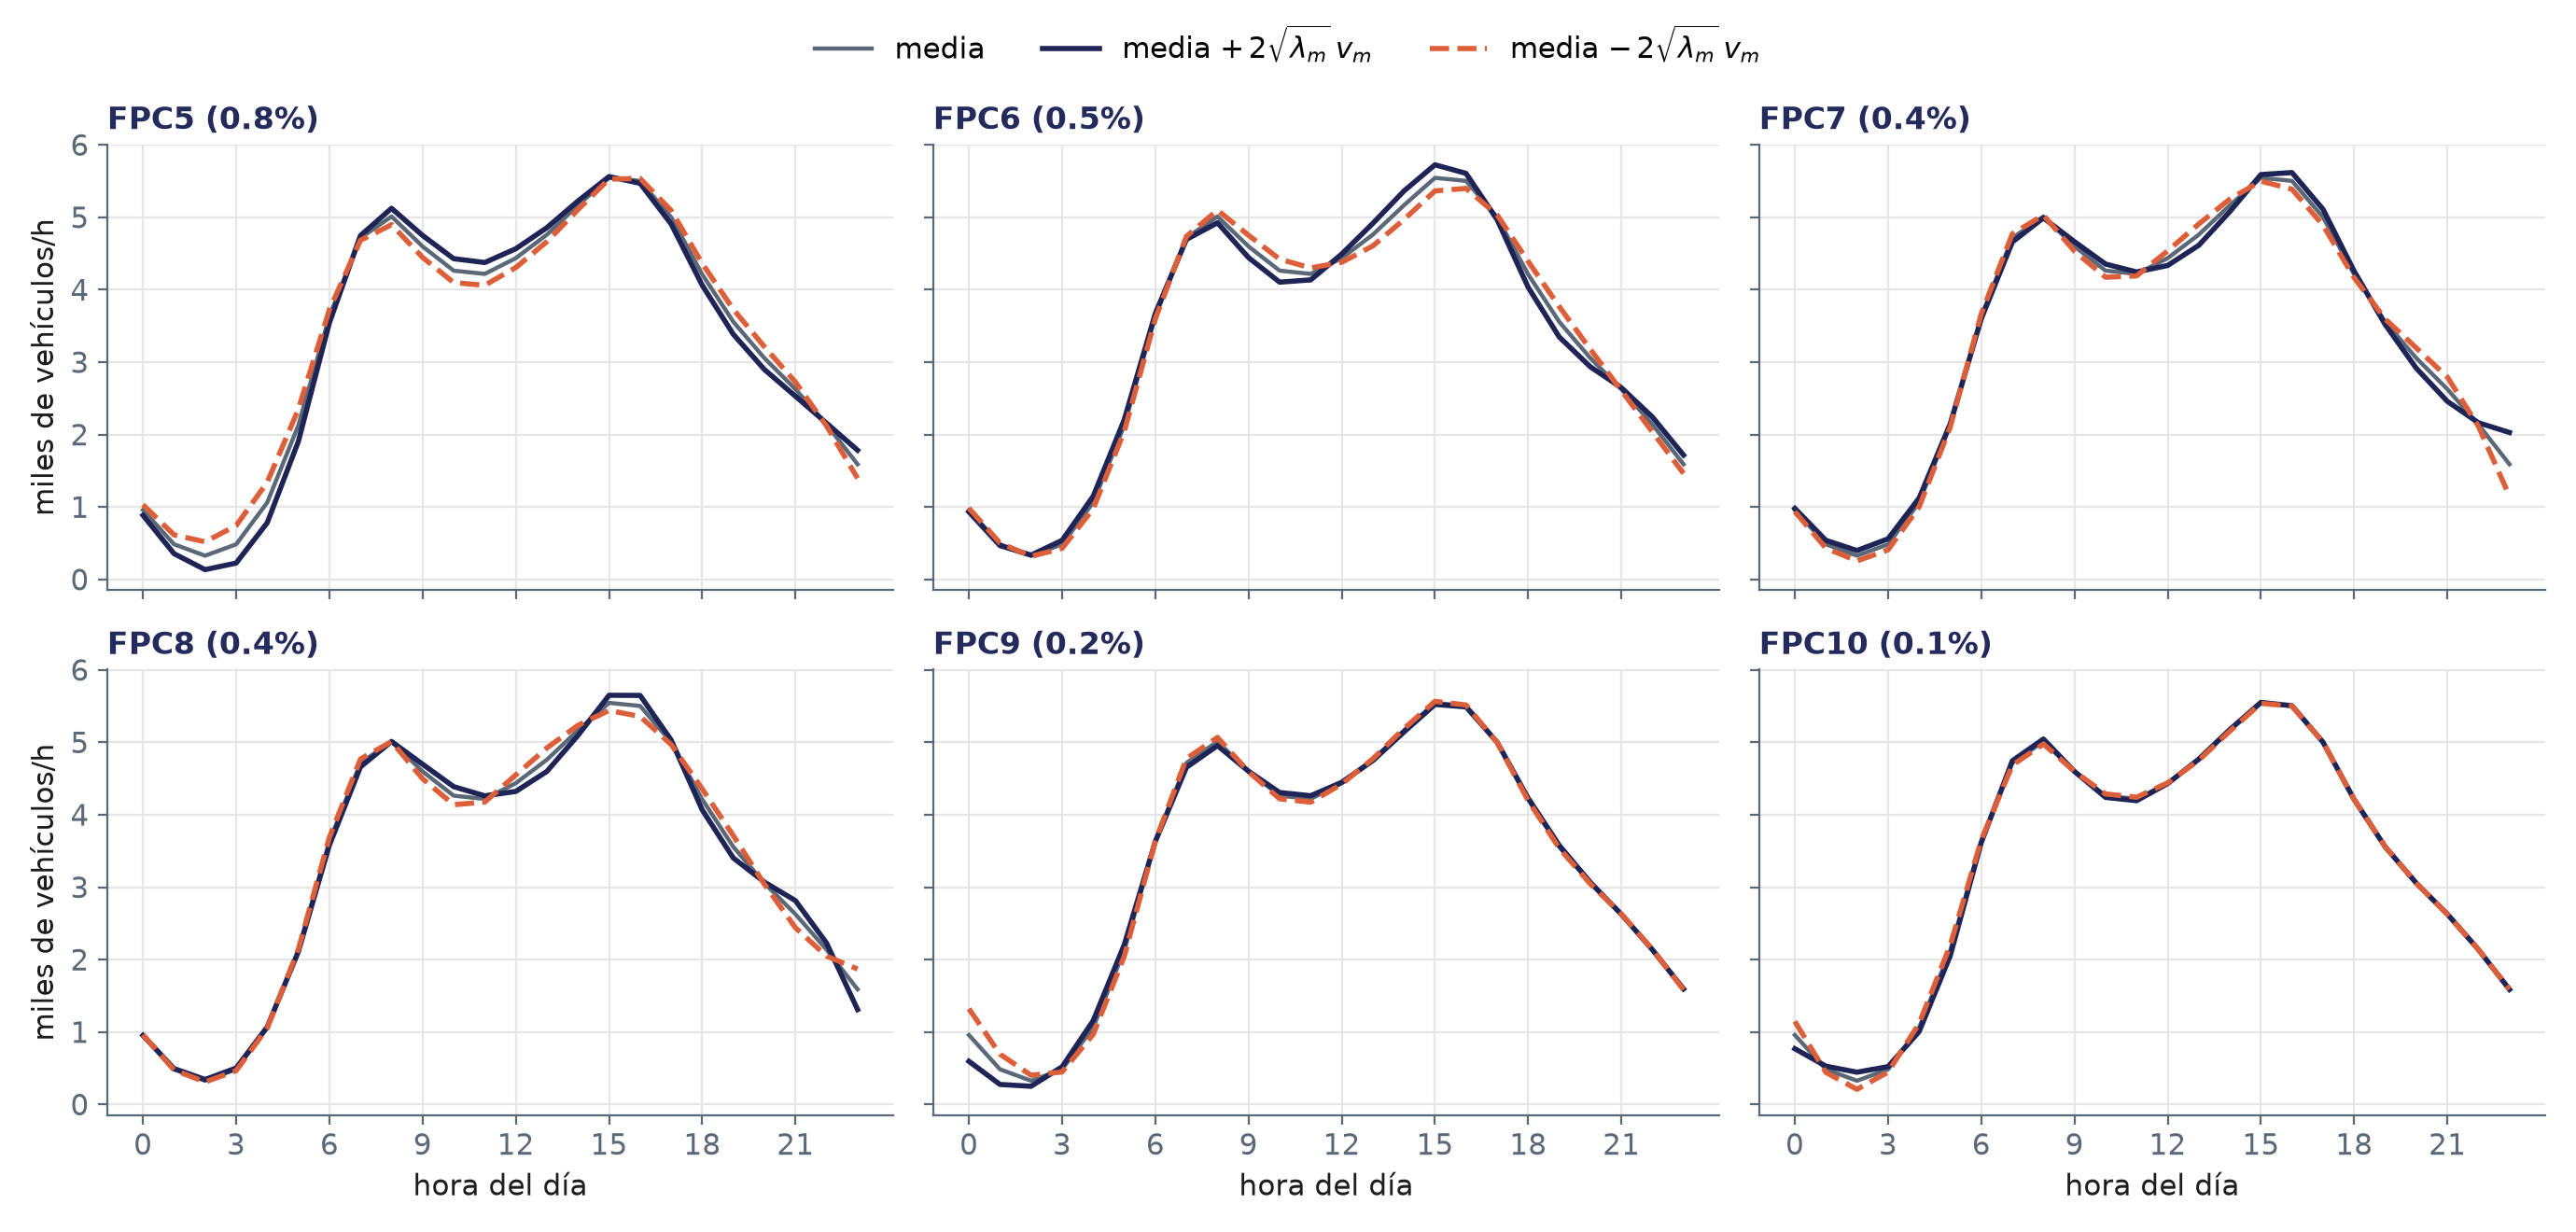
\includegraphics[width=\textwidth,height=0.6\textheight,keepaspectratio]{IMG/aneC_00/aneC_00_autofunciones_menores.png}
\caption{Curva media del bloque de entrenamiento y su perturbación $\mu \pm 2\sqrt{\lambda_m}\,v_m$ a lo largo de las autofunciones $5$ a $10$.}
\label{fig:aneC_autofunciones_menores}
\end{figure}

Las autofunciones menores (Figura~\ref{fig:aneC_autofunciones_menores}) son ajustes locales del perfil, de una amplitud de unos cientos de vehículos por hora frente a los miles de las cuatro primeras (Figura~\ref{fig:aneC_autofunciones}). La quinta mueve la madrugada, entre la una y las cinco, frente a la media mañana; la sexta desplaza la punta de la tarde hacia antes o después de las dieciséis horas; la séptima y la octava ajustan el cierre de la tarde y la noche, y la novena y la décima se concentran en las primeras horas del día, en el borde del dominio.

\begin{table}[H]
\centering\small
\setlength{\tabcolsep}{4pt}
\caption{Ocupación de la mezcla y selección de cada score ($M = 10$): fracción de la varianza, índice medio del último átomo ocupado ($N_1$, sobre 30), número de covariables con PIP mayor que $0.5$ y PIP mínima, con rezago $\{1\}$ (diez covariables) y rezagos $\{1,7\}$ (diez de cada rezago).}
\label{tab:aneC_pip}
\begin{tabular}{l c ccc cccc}
\hline
 & & \multicolumn{3}{c}{Rezago $\{1\}$} & \multicolumn{4}{c}{Rezagos $\{1,7\}$} \\
 & & & \multicolumn{2}{c}{PIP} & & \multicolumn{3}{c}{PIP} \\
Score & Var. (\%) & $N_1$ & $> 0.5$ & mín. & $N_1$ & $> 0.5$, $t-1$ & $> 0.5$, $t-7$ & mín. \\
\hline
$\xi_{t1}$  & 79.9 & 8.7  & 5 & 0.06 & 10.3 & 4  & 2  & 0.10 \\
$\xi_{t2}$  & 12.4 & 15.2 & 4 & 0.16 & 15.3 & 5  & 3  & 0.41 \\
$\xi_{t3}$  & 3.7  & 14.5 & 3 & 0.10 & 19.5 & 10 & 10 & 0.67 \\
$\xi_{t4}$  & 1.7  & 16.4 & 7 & 0.32 & 20.7 & 8  & 9  & 0.47 \\
$\xi_{t5}$  & 0.8  & 16.8 & 5 & 0.31 & 10.0 & 3  & 4  & 0.29 \\
$\xi_{t6}$  & 0.5  & 22.3 & 2 & 0.12 & 29.9 & 10 & 10 & 0.94 \\
$\xi_{t7}$  & 0.4  & 24.7 & 2 & 0.09 & 28.2 & 10 & 10 & 0.81 \\
$\xi_{t8}$  & 0.4  & 27.9 & 2 & 0.04 & 30.0 & 10 & 10 & 0.91 \\
$\xi_{t9}$  & 0.2  & 21.4 & 6 & 0.31 & 23.1 & 10 & 10 & 0.75 \\
$\xi_{t10}$ & 0.1  & 14.2 & 2 & 0.14 & 29.1 & 10 & 10 & 0.86 \\
\hline
\end{tabular}
\end{table}

El Cuadro~\ref{tab:aneC_pip} separa dos situaciones. Con el rezago de un día las mezclas de los scores menores son escasas aunque ocupen muchos átomos, pues las de los scores $6$, $7$, $8$ y $10$ incluyen solo dos covariables, su propio rezago y el de un score principal (el cuarto en el sexto, el primero en el séptimo y el octavo, y el tercero en el décimo), y dejan las demás en $0.47$ o menos. Con el rezago semanal, en cambio, las mezclas del tercer score y de los scores $6$ a $10$ ocupan entre 20 y 30 átomos y todas sus covariables superan $0.5$, con mínimos entre $0.67$ y $0.94$. La selección escasa se conserva solo en las mezclas que usan pocos átomos, las de los scores $1$, $2$ y $5$, con $N_1$ entre 10 y 15. La PIP de las mezclas que llenan el truncamiento refleja el número de átomos ocupados más que la relevancia de cada covariable, y por eso no se interpreta.

\chapter{Resultados de las Otras Series Reales}
\label{aneD_00_00_otras_series}

% Corridas 103-107 de notebooks/reales/, M = 10, test, w = 30. Cuadros desde reports/reales/<eid>_barrido_M/{98,99,102}_*
% y <eid>_m10/{72,81}_ventana_*_w30.csv (scratchpad tablas_aneD.py); figuras con el estilo del Capítulo 3 (figuras_aneD.py).

Este anexo reúne los resultados del PSBPM-FD en otras cinco series reales de curvas diarias, ajustadas con la misma configuración que el tráfico con el rezago de un día (Capítulo~\ref{04_00_00_aplicacion}). A diferencia del tráfico, ninguna de ellas tiene un estado oculto que separe perfiles distintos de la curva siguiente, y en todas la predictiva resultó unimodal. Se reportan el error puntual, los intervalos de predicción y, brevemente, los comportamientos predictivos. Salvo indicación, las cifras corresponden a $M = 10$, al bloque de prueba y a la ventana móvil de ancho $w = 30$.

\section{Series y configuración}
\label{aneD_00_01_series}

El Cuadro~\ref{tab:aneD_series} describe las series. Cada día es una curva observada en $G$ instantes, a la que se aplica, cuando se indica, una transformación que estabiliza su escala, y las métricas se calculan en la escala transformada. La configuración es la del tráfico con el rezago de un día (Cuadro~\ref{tab:aneC_configuracion}) con base B-spline cúbica de $K = 10$ funciones con el mismo tratamiento de los huecos, FPCA estimada con el bloque de entrenamiento, $M = 10$ componentes, los diez scores del día anterior como covariables de cada score, $a_\nu = 2$, inclusión a priori $(1, 5)$ y una cadena de 2500 iteraciones con 30 átomos. La única diferencia es el calentamiento, de 500 iteraciones en lugar de 1000. Las referencias son el FAR(1), con su banda gaussiana, y el Random Forest con las mismas covariables.

% Fuente: datasets_manifest.json y 65_comportamientos_calendario.csv de cada corrida; descripción de la curva en el _01.
\begin{table}[H]
\centering\small
\setlength{\tabcolsep}{3.5pt}
\caption{Series reales adicionales: variable de la curva diaria, número de instantes por día ($G$), período, número de días ($T$) y partición en entrenamiento y prueba.}
\label{tab:aneD_series}
\begin{tabular}{l p{0.32\textwidth} c c c c}
\hline
Serie & Curva diaria & $G$ & Período & $T$ & Entren. / prueba \\
\hline
Precio SA1 & Precio spot de la región Australia del Sur del mercado eléctrico australiano (AEMO), $\operatorname{asinh}(\text{precio}/100)$, cada 5 minutos & 288 & 2022--2025 & 1461 & 1096 / 365 \\
PM2.5 O'Higgins & Concentración horaria de PM2.5 en la estación Parque O'Higgins de Santiago (SINCA), $\log(1 + x)$ & 24 & 2015--2025 & 4018 & 2922 / 1096 \\
PM2.5 Beijing & Concentración horaria de PM2.5, promedio de doce estaciones de Beijing, $\log(1 + x)$ & 24 & 2013--2017 & 1461 & 1022 / 439 \\
Eólica & Factor de planta de la generación eólica terrestre de Alemania (SMARD), cada 15 minutos & 96 & 2015--2026 & 4299 & 3009 / 1290 \\
Volatilidad BTC & Mitad del logaritmo de la varianza realizada horaria de BTCUSDT (Binance), con retornos de 5 minutos & 24 & 2020--2026 & 2435 & 1704 / 731 \\
\hline
\end{tabular}
\end{table}

\section{Error puntual}
\label{aneD_00_02_error_puntual}

Los Cuadros~\ref{tab:aneD_bloqueA} a~\ref{tab:aneD_bloqueA_gana} resumen el MAE y el RMSE de los tres predictores del PSBPM-FD y de las dos referencias, como en la Sección~\ref{04_03_01_error_puntual}. Como las escalas de las series son distintas, las cifras se comparan dentro de cada fila y no entre series.

% Fuente: 98_resumen_bloqueA_min_max_prom.csv del barrido (test, M = 10, promedio sobre ventanas).
\begin{table}[H]
\centering\footnotesize
\setlength{\tabcolsep}{2.5pt}
\caption{MAE y RMSE en el bloque de prueba por serie ($M = 10$, $w = 30$). En negrita el menor de cada métrica.}
\label{tab:aneD_bloqueA}
\begin{tabular}{l ccccc ccccc}
\hline
 & \multicolumn{5}{c}{MAE} & \multicolumn{5}{c}{RMSE} \\
Serie & Esp. & Med. & Modal & RF & FAR & Esp. & Med. & Modal & RF & FAR \\
\hline
Precio SA1 & \textbf{0.3279} & 0.3286 & 0.3438 & 0.3415 & 0.3280 & \textbf{0.4417} & 0.4430 & 0.4666 & 0.4528 & 0.4418 \\
PM2.5 O'Higgins & \textbf{0.3166} & 0.3168 & 0.3327 & 0.3281 & 0.3214 & \textbf{0.4300} & 0.4311 & 0.4526 & 0.4459 & 0.4347 \\
PM2.5 Beijing & 0.5664 & 0.5515 & 0.5786 & 0.5957 & \textbf{0.5506} & 0.7445 & 0.7503 & 0.8385 & 0.7606 & \textbf{0.7390} \\
Eólica & 0.0859 & \textbf{0.0853} & 0.0993 & 0.0961 & 0.0857 & \textbf{0.1191} & 0.1196 & 0.1368 & 0.1270 & 0.1197 \\
Volatilidad BTC & 0.3288 & 0.3303 & 0.3489 & 0.3292 & \textbf{0.3242} & 0.4229 & 0.4247 & 0.4466 & 0.4230 & \textbf{0.4184} \\
\hline
\end{tabular}
\end{table}

\begin{table}[H]
\centering\small
\setlength{\tabcolsep}{3.5pt}
\caption{Cambio relativo del MAE y del RMSE respecto del FAR por predictor y serie. Negativo es mejor que el FAR.}
\label{tab:aneD_bloqueA_ganancia}
\begin{tabular}{l cc cc cc cc}
\hline
 & \multicolumn{2}{c}{Esperanza} & \multicolumn{2}{c}{Mediana} & \multicolumn{2}{c}{Modal} & \multicolumn{2}{c}{Random Forest} \\
Serie & MAE & RMSE & MAE & RMSE & MAE & RMSE & MAE & RMSE \\
\hline
Precio SA1 & $0.0\%$ & $0.0\%$ & $+0.2\%$ & $+0.3\%$ & $+4.8\%$ & $+5.6\%$ & $+4.1\%$ & $+2.5\%$ \\
PM2.5 O'Higgins & $-1.5\%$ & $-1.1\%$ & $-1.4\%$ & $-0.8\%$ & $+3.5\%$ & $+4.1\%$ & $+2.1\%$ & $+2.6\%$ \\
PM2.5 Beijing & $+2.9\%$ & $+0.7\%$ & $+0.2\%$ & $+1.5\%$ & $+5.1\%$ & $+13.5\%$ & $+8.2\%$ & $+2.9\%$ \\
Eólica & $+0.3\%$ & $-0.5\%$ & $-0.4\%$ & $-0.1\%$ & $+15.9\%$ & $+14.3\%$ & $+12.1\%$ & $+6.1\%$ \\
Volatilidad BTC & $+1.4\%$ & $+1.1\%$ & $+1.9\%$ & $+1.5\%$ & $+7.6\%$ & $+6.7\%$ & $+1.5\%$ & $+1.1\%$ \\
\hline
\end{tabular}
\end{table}

% Fuente: 72_ventana_modelos_w30.csv (test, sin ventanas que cruzan T0, sin el medoide).
\begin{table}[H]
\centering\small
\setlength{\tabcolsep}{3.5pt}
\caption{Fracción de ventanas de prueba que gana cada modelo, por MAE y por RMSE.}
\label{tab:aneD_bloqueA_ventanas}
\begin{tabular}{l ccccc ccccc}
\hline
 & \multicolumn{5}{c}{MAE} & \multicolumn{5}{c}{RMSE} \\
Serie & FAR & RF & Esp. & Med. & Modal & FAR & RF & Esp. & Med. & Modal \\
\hline
Precio SA1 & 45\% & 16\% & 23\% & 11\% & 4\% & 48\% & 25\% & 22\% & 4\% & 1\% \\
PM2.5 O'Higgins & 22\% & 17\% & 31\% & 26\% & 4\% & 25\% & 19\% & 28\% & 26\% & 1\% \\
PM2.5 Beijing & 40\% & 9\% & 5\% & 29\% & 19\% & 45\% & 14\% & 23\% & 17\% & 0\% \\
Eólica & 39\% & 4\% & 12\% & 40\% & 6\% & 34\% & 9\% & 23\% & 29\% & 5\% \\
Volatilidad BTC & 52\% & 28\% & 17\% & 2\% & 1\% & 50\% & 32\% & 14\% & 3\% & 0\% \\
\hline
\end{tabular}
\end{table}

\begin{table}[H]
\centering\small
\setlength{\tabcolsep}{3.5pt}
\caption{Fracción de ventanas de prueba en que el predictor consistente del PSBPM-FD supera a cada referencia: la mediana puntual bajo MAE y la esperanza bajo RMSE.}
\label{tab:aneD_bloqueA_gana}
\begin{tabular}{l cc cc}
\hline
 & \multicolumn{2}{c}{MAE (mediana puntual)} & \multicolumn{2}{c}{RMSE (esperanza)} \\
Serie & vs FAR & vs RF & vs FAR & vs RF \\
\hline
Precio SA1 & 41\% & 82\% & 43\% & 74\% \\
PM2.5 O'Higgins & 69\% & 77\% & 67\% & 79\% \\
PM2.5 Beijing & 54\% & 86\% & 43\% & 74\% \\
Eólica & 55\% & 95\% & 56\% & 90\% \\
Volatilidad BTC & 18\% & 46\% & 23\% & 52\% \\
\hline
\end{tabular}
\end{table}

En el error puntual la esperanza y la mediana puntual del PSBPM-FD quedan a menos de un $3\%$ del FAR en todas las series. La ventaja más clara es la del PM2.5 de Parque O'Higgins, donde la esperanza baja el MAE y el RMSE del FAR en un $1.5\%$ y un $1.1\%$ y el predictor consistente le gana en dos de cada tres ventanas. En el precio SA1 y en la eólica el empate es casi exacto, con diferencias de medio punto porcentual o menos, mientras que en el PM2.5 de Beijing y en la volatilidad de BTC el FAR es el mejor, con la mayor distancia en la volatilidad, donde la mediana puntual le gana solo en el $18\%$ de las ventanas. Como las predictivas son unimodales, la esperanza y la mediana puntual casi coinciden, y solo en Beijing se separan, con una mediana que baja el MAE de la esperanza en un $2.6\%$, señal de una predictiva asimétrica. El átomo más probable es el peor predictor del PSBPM-FD en todas las series, como en el estudio de simulación. El Random Forest queda por detrás del FAR en las cinco series, y el predictor consistente del PSBPM-FD lo supera en la mayoría de las ventanas salvo en la volatilidad de BTC, donde ambos empatan.

% Fuente: 72_ventana_modelos_w30.csv de cada serie (test).
\begin{figure}[H]
\centering
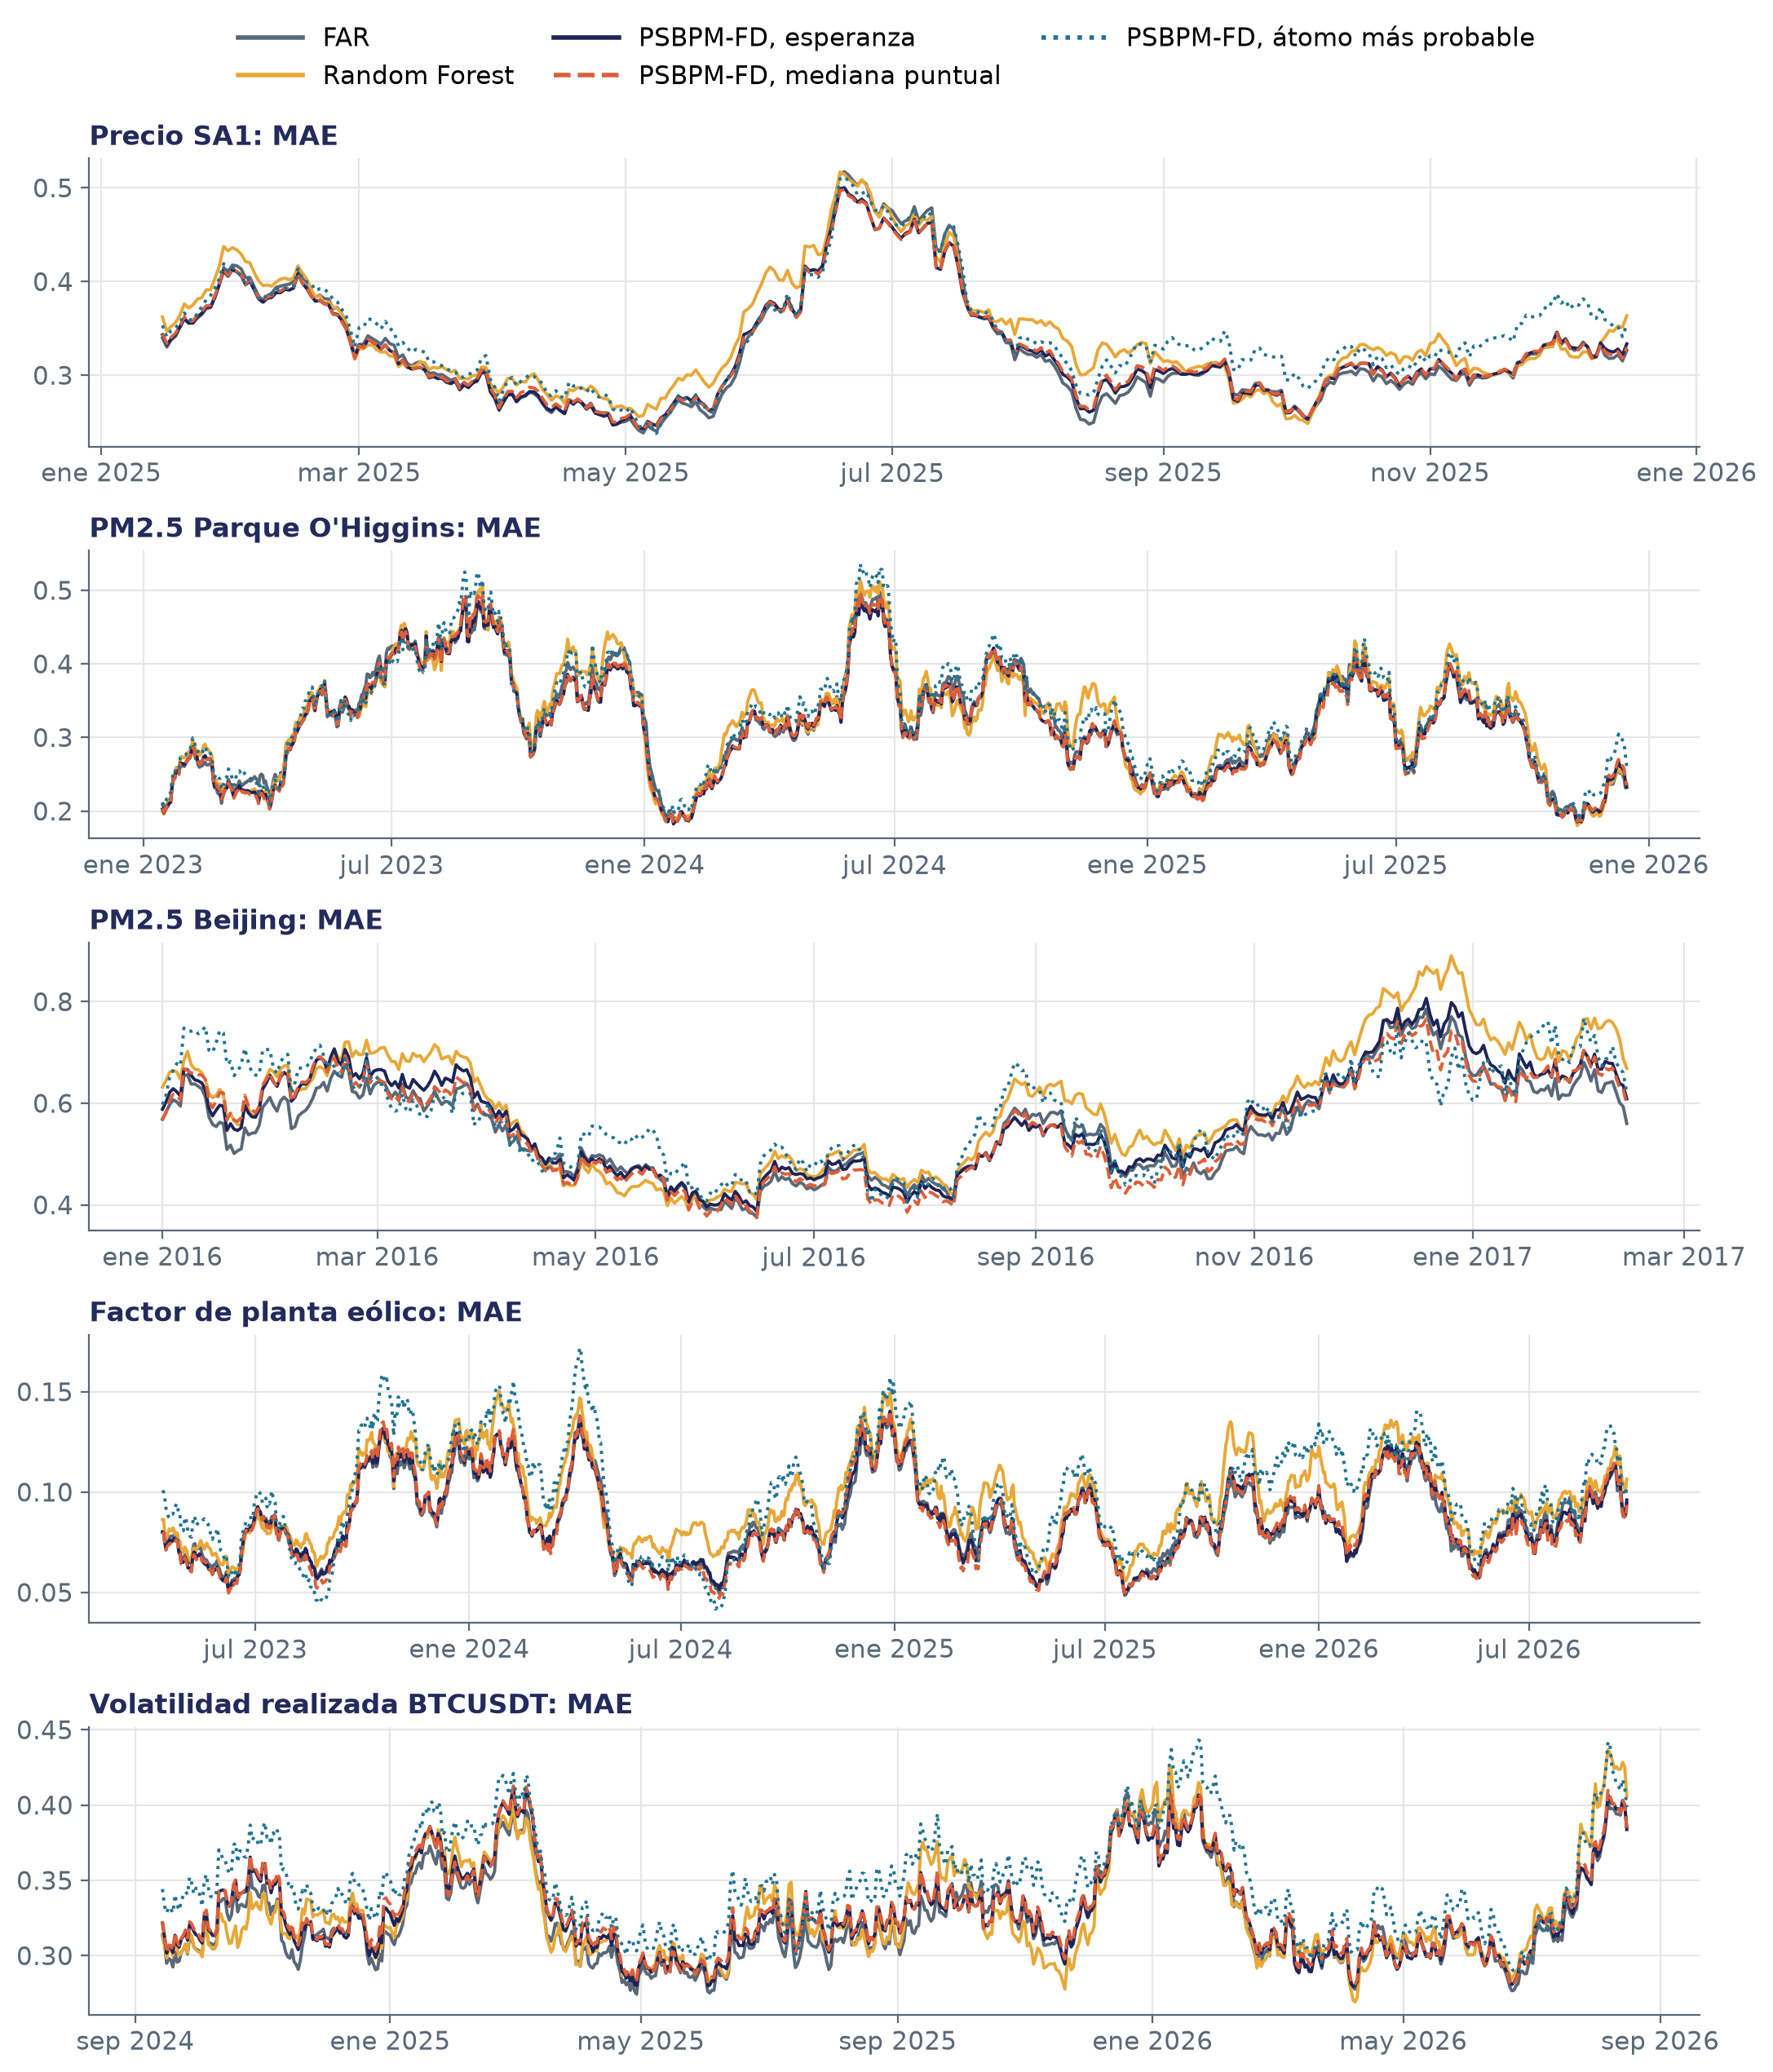
\includegraphics[width=\textwidth,height=0.85\textheight,keepaspectratio]{IMG/aneD_00/aneD_00_ventana_mae_w30.png}
\caption{MAE sobre la ventana móvil del bloque de prueba de los tres predictores del PSBPM-FD, el FAR y el Random Forest, por serie ($M = 10$, $w = 30$).}
\label{fig:aneD_ventana_mae}
\end{figure}

La Figura~\ref{fig:aneD_ventana_mae} muestra que las curvas de error de los cinco modelos se mueven juntas en todas las series: los períodos difíciles, como los meses de precios altos de junio y julio de 2025 en la SA1, los inviernos en las dos series de PM2.5 y en la eólica, lo son para todos los modelos, y las diferencias entre ellos son pequeñas frente a la variación del error a lo largo del bloque de prueba.

\section{Intervalos de predicción}
\label{aneD_00_03_intervalos}

Los Cuadros~\ref{tab:aneD_bloqueB_winkler} a~\ref{tab:aneD_bloqueB_ventanas} comparan las tres construcciones de intervalo del PSBPM-FD con la banda gaussiana del FAR, como en la Sección~\ref{04_03_02_intervalos}.

% Fuente: 99_resumen_bloqueB_min_max_prom.csv del barrido (test, M = 10).
\begin{table}[H]
\centering\small
\setlength{\tabcolsep}{3.5pt}
\caption{Winkler y MPIW en el bloque de prueba por serie y construcción ($M = 10$, $w = 30$). En negrita el menor Winkler de cada serie.}
\label{tab:aneD_bloqueB_winkler}
\begin{tabular}{l cccc cccc}
\hline
 & \multicolumn{4}{c}{Winkler} & \multicolumn{4}{c}{MPIW} \\
Serie & FAR & Equi. & HDR & Simult. & FAR & Equi. & HDR & Simult. \\
\hline
Precio SA1 & 2.374 & \textbf{2.354} & 2.361 & 2.977 & 1.872 & 1.881 & 1.885 & 2.870 \\
PM2.5 O'Higgins & 2.484 & \textbf{2.421} & 2.441 & 2.696 & 1.645 & 1.692 & 1.687 & 2.450 \\
PM2.5 Beijing & 3.883 & \textbf{3.522} & 3.717 & 4.169 & 2.710 & 2.852 & 2.847 & 3.986 \\
Eólica & \textbf{0.581} & 0.605 & 0.622 & 0.730 & 0.454 & 0.488 & 0.487 & 0.674 \\
Volatilidad BTC & \textbf{2.075} & 2.076 & 2.075 & 2.608 & 1.634 & 1.735 & 1.739 & 2.597 \\
\hline
\end{tabular}
\end{table}

\begin{table}[H]
\centering\small
\setlength{\tabcolsep}{3.5pt}
\caption{PICP y PICPB en el bloque de prueba por serie y construcción ($M = 10$, $w = 30$). Nivel nominal $0.95$.}
\label{tab:aneD_bloqueB_picp}
\begin{tabular}{l cccc cccc}
\hline
 & \multicolumn{4}{c}{PICP} & \multicolumn{4}{c}{PICPB} \\
Serie & FAR & Equi. & HDR & Simult. & FAR & Equi. & HDR & Simult. \\
\hline
Precio SA1 & 0.956 & 0.956 & 0.956 & 0.994 & 0.717 & 0.696 & 0.702 & 0.947 \\
PM2.5 O'Higgins & 0.937 & 0.942 & 0.941 & 0.981 & 0.676 & 0.686 & 0.696 & 0.901 \\
PM2.5 Beijing & 0.933 & 0.939 & 0.933 & 0.980 & 0.786 & 0.763 & 0.763 & 0.926 \\
Eólica & 0.946 & 0.955 & 0.956 & 0.985 & 0.783 & 0.808 & 0.825 & 0.940 \\
Volatilidad BTC & 0.944 & 0.954 & 0.955 & 0.995 & 0.633 & 0.673 & 0.677 & 0.951 \\
\hline
\end{tabular}
\end{table}

\begin{table}[H]
\centering\small
\setlength{\tabcolsep}{3pt}
\caption{Cambio relativo del Winkler y del MPIW respecto del FAR por serie y construcción. Negativo es mejor que el FAR.}
\label{tab:aneD_bloqueB_ganancia}
\begin{tabular}{l cc cc cc}
\hline
 & \multicolumn{2}{c}{Equi-colas} & \multicolumn{2}{c}{Máxima densidad} & \multicolumn{2}{c}{Simultánea} \\
Serie & Winkler & MPIW & Winkler & MPIW & Winkler & MPIW \\
\hline
Precio SA1 & $-0.8\%$ & $+0.5\%$ & $-0.5\%$ & $+0.7\%$ & $+25.4\%$ & $+53.3\%$ \\
PM2.5 O'Higgins & $-2.5\%$ & $+2.9\%$ & $-1.7\%$ & $+2.5\%$ & $+8.5\%$ & $+48.9\%$ \\
PM2.5 Beijing & $-9.3\%$ & $+5.3\%$ & $-4.3\%$ & $+5.1\%$ & $+7.4\%$ & $+47.1\%$ \\
Eólica & $+4.2\%$ & $+7.5\%$ & $+7.0\%$ & $+7.2\%$ & $+25.7\%$ & $+48.5\%$ \\
Volatilidad BTC & $+0.1\%$ & $+6.2\%$ & $0.0\%$ & $+6.4\%$ & $+25.7\%$ & $+59.0\%$ \\
\hline
\end{tabular}
\end{table}

% Fuente: 81_ventana_bloqueB_w30.csv (test, sin ventanas que cruzan T0).
\begin{table}[H]
\centering\small
\setlength{\tabcolsep}{3.5pt}
\caption{Fracción de ventanas de prueba en que cada banda tiene el menor Winkler, y en que cada banda del PSBPM-FD tiene un Winkler menor que el del FAR.}
\label{tab:aneD_bloqueB_ventanas}
\begin{tabular}{l cccc ccc}
\hline
 & \multicolumn{4}{c}{La mejor banda} & \multicolumn{3}{c}{Gana al FAR} \\
Serie & FAR & Equi. & HDR & Simult. & Equi. & HDR & Simult. \\
\hline
Precio SA1 & 39\% & 35\% & 19\% & 7\% & 60\% & 52\% & 8\% \\
PM2.5 O'Higgins & 32\% & 35\% & 16\% & 17\% & 61\% & 57\% & 24\% \\
PM2.5 Beijing & 20\% & 78\% & 3\% & 0\% & 80\% & 68\% & 28\% \\
Eólica & 64\% & 20\% & 16\% & 1\% & 34\% & 30\% & 1\% \\
Volatilidad BTC & 53\% & 25\% & 21\% & 0\% & 44\% & 42\% & 2\% \\
\hline
\end{tabular}
\end{table}

En los intervalos el resultado depende de la serie. La banda equi-colas del PSBPM-FD baja el Winkler del FAR en tres de las cinco series: con claridad en el PM2.5 de Beijing, un $9.3\%$ y en el $80\%$ de las ventanas, y por poco en el PM2.5 de Parque O'Higgins y en el precio SA1, un $2.5\%$ y un $0.8\%$, en alrededor del $60\%$ de las ventanas. En la volatilidad de BTC empatan, y en la eólica el FAR es mejor, un $4\%$ y en dos de cada tres ventanas. La banda del PSBPM-FD es algo más ancha que la del FAR en todas las series, entre un $0.5\%$ y un $7.5\%$ en MPIW, de modo que donde gana el Winkler lo hace porque la penalización por no cubrir la curva baja más de lo que sube el ancho. La banda de máxima densidad queda cerca de la equi-colas, porque con predictivas unimodales ambas construcciones se parecen, y se separa sobre todo en Beijing, la serie de predictiva asimétrica. La banda simultánea es la única que se acerca al nivel nominal en el PICPB, entre $0.90$ y $0.95$, frente a valores entre $0.63$ y $0.83$ de las bandas puntuales, y paga esa cobertura con un ancho cerca de un $50\%$ mayor y el peor Winkler en todas las series.

% Fuente: 81_ventana_bloqueB_w30.csv de cada serie (test).
\begin{figure}[H]
\centering
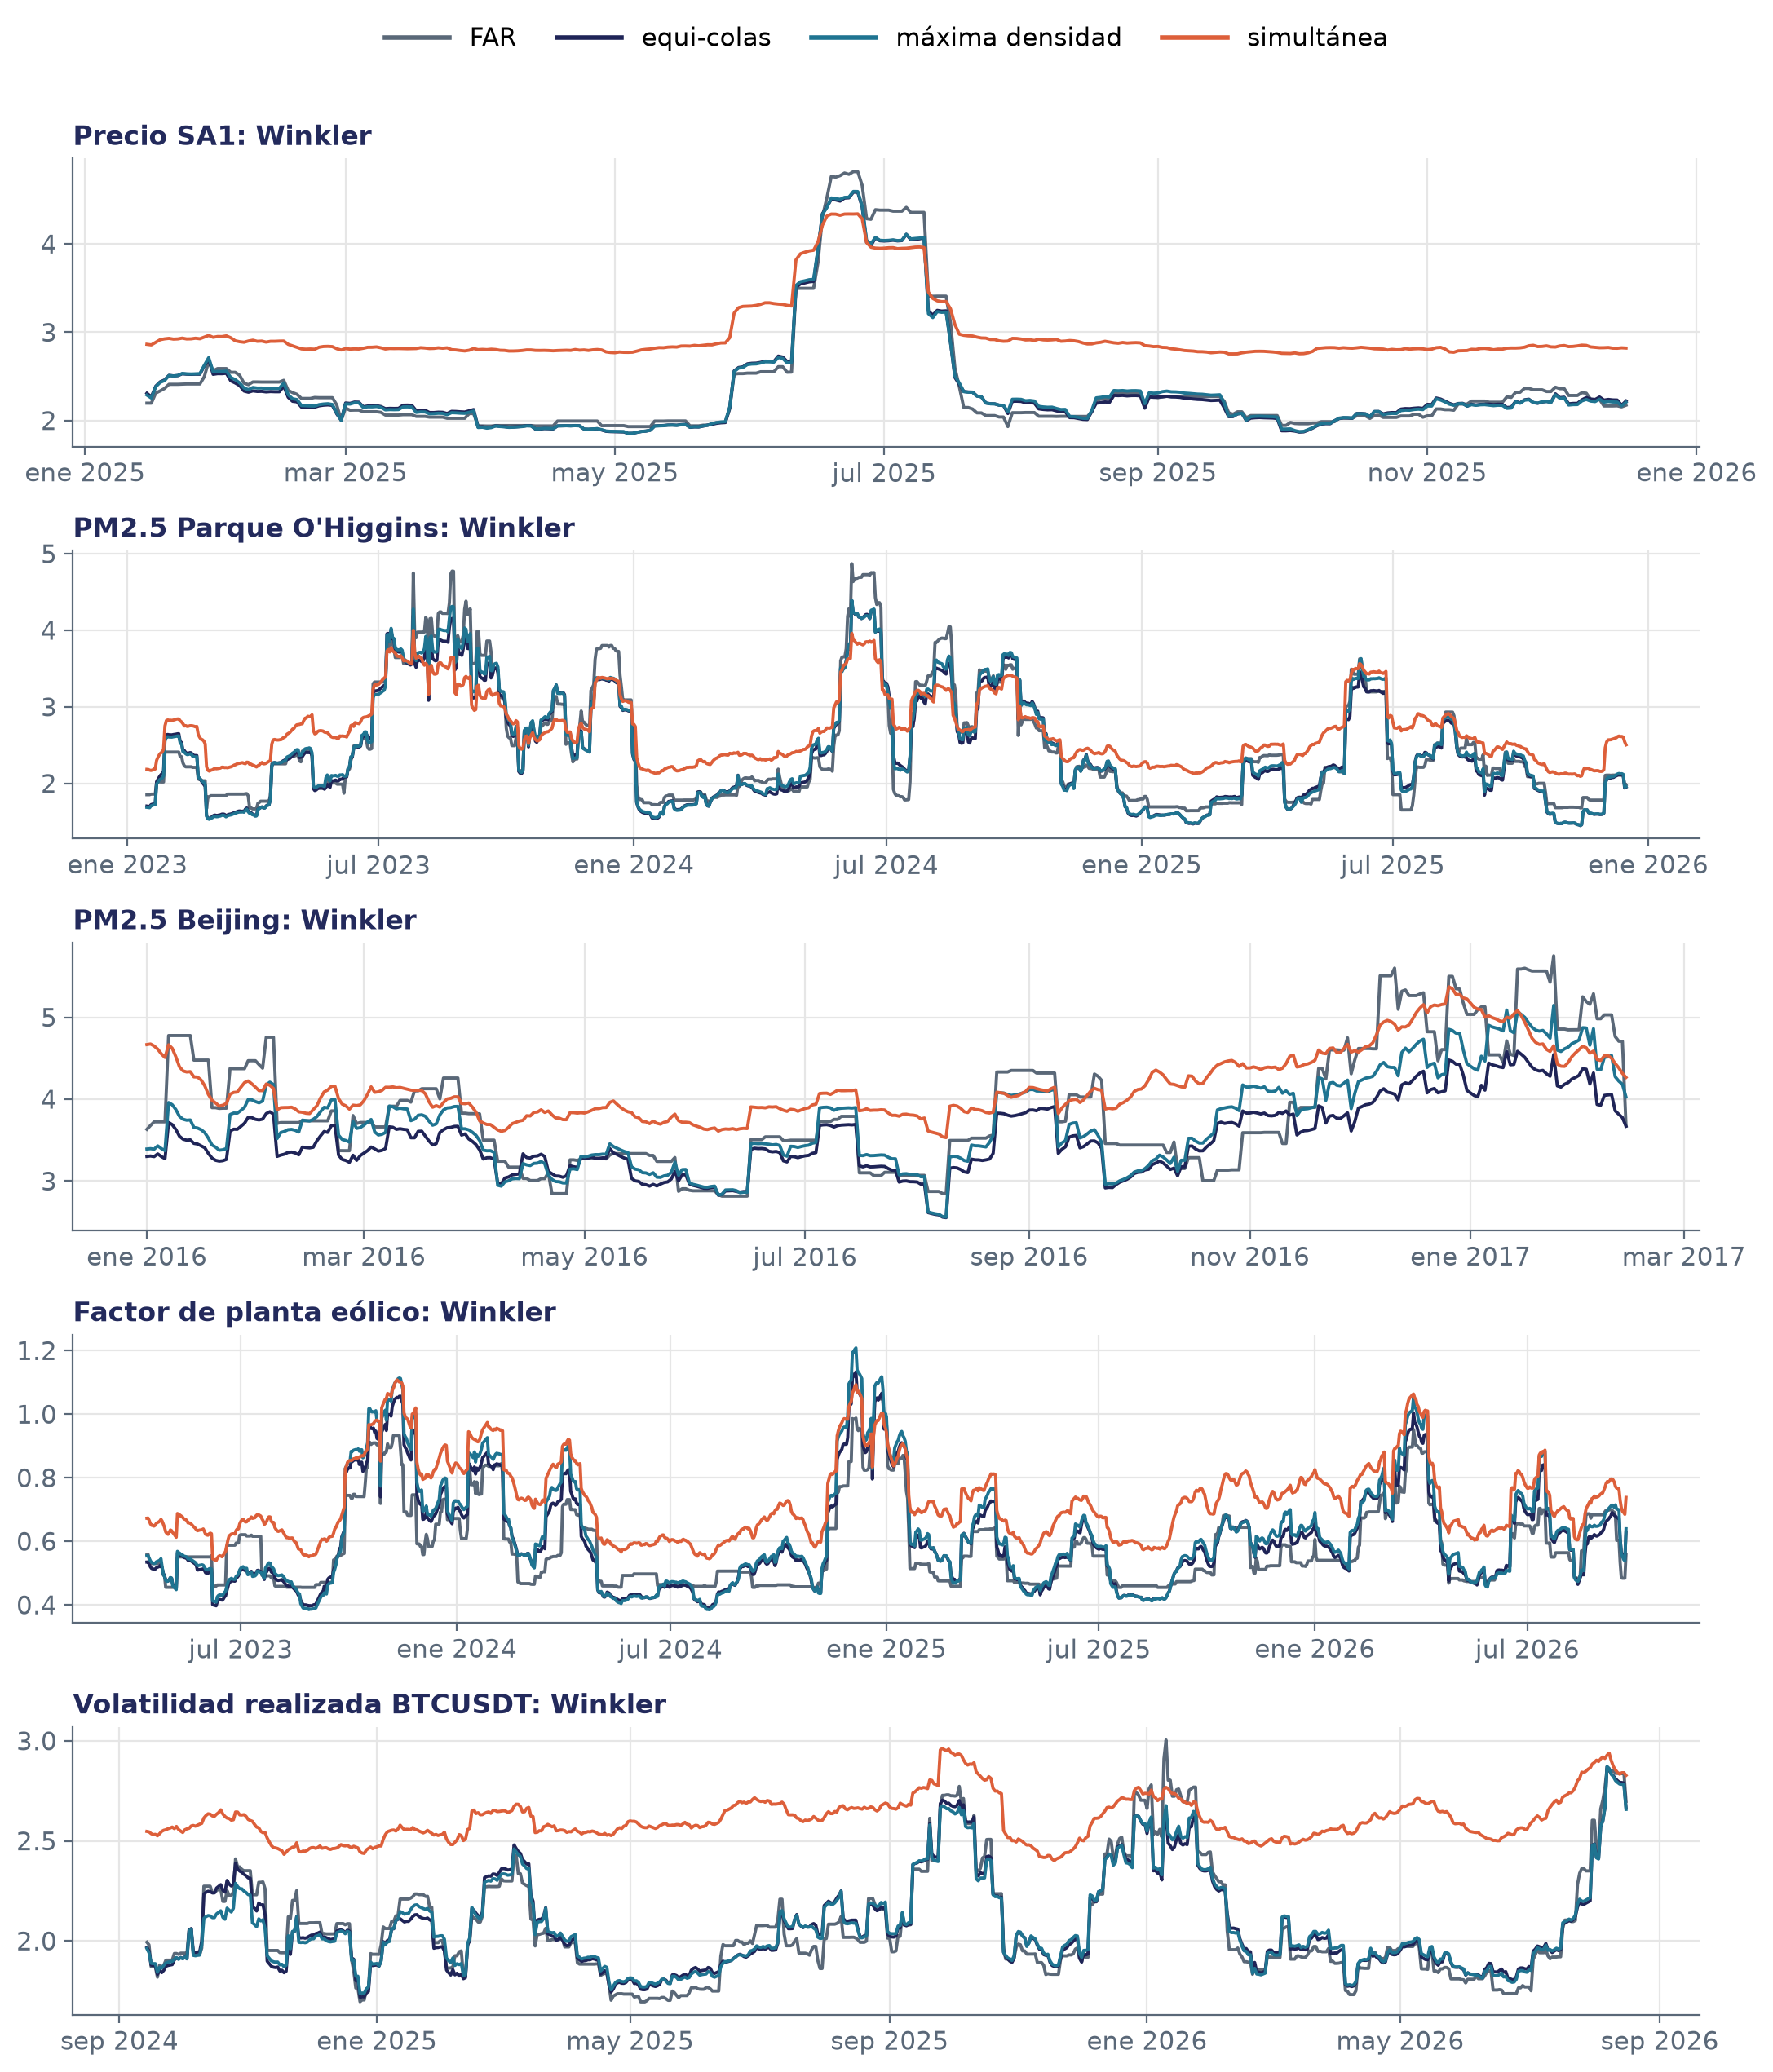
\includegraphics[width=\textwidth,height=0.85\textheight,keepaspectratio]{IMG/aneD_00/aneD_00_ventana_winkler_w30.png}
\caption{Winkler sobre la ventana móvil del bloque de prueba de las tres construcciones del PSBPM-FD y de la banda del FAR, por serie ($M = 10$, $w = 30$).}
\label{fig:aneD_ventana_winkler}
\end{figure}

La Figura~\ref{fig:aneD_ventana_winkler} muestra dónde se produce la diferencia. En el PM2.5 de Beijing la banda equi-colas queda bajo la del FAR en la mayor parte del bloque de prueba, con la mayor distancia en los dos inviernos. En el precio SA1 y en el PM2.5 de Parque O'Higgins las bandas del PSBPM-FD quedan bajo la del FAR en los tramos de mayor Winkler, los meses de precios altos de 2025 en la SA1 y los inviernos en Santiago, y se confunden con ella en el resto. En la eólica, en cambio, la banda del FAR es la mejor en dos de cada tres ventanas, repartidas a lo largo del bloque, y en la volatilidad de BTC las bandas puntuales no se distinguen.

\section{Comportamientos predictivos}
\label{aneD_00_04_comportamientos}

El Cuadro~\ref{tab:aneD_K} resume cuántos comportamientos declara el modelo en el bloque de prueba de cada serie.

% Fuente: 102_K_por_M.csv del barrido (test, M = 10); fechas de los orígenes con K = 2 en 65_comportamientos_calendario.csv.
\begin{table}[H]
\centering\small
\setlength{\tabcolsep}{3.5pt}
\caption{Distribución de $K_t$ en el bloque de prueba por serie ($M = 10$) y número de orígenes con más de un comportamiento.}
\label{tab:aneD_K}
\begin{tabular}{l c ccc c}
\hline
Serie & Orígenes & $K_t = 1$ & $K_t = 2$ & $K_t \ge 3$ & Orígenes con $K_t \ge 2$ \\
\hline
Precio SA1 & 365 & 99.7\% & 0.3\% & 0.0\% & 1 \\
PM2.5 O'Higgins & 1096 & 99.5\% & 0.5\% & 0.0\% & 5 \\
PM2.5 Beijing & 439 & 100.0\% & 0.0\% & 0.0\% & 0 \\
Eólica & 1290 & 99.9\% & 0.1\% & 0.0\% & 1 \\
Volatilidad BTC & 731 & 100.0\% & 0.0\% & 0.0\% & 0 \\
\hline
\end{tabular}
\end{table}

En las cinco series la predictiva tiene un solo comportamiento en al menos el $99.5\%$ de los orígenes de prueba, y en Beijing y en la volatilidad de BTC en todos. Los pocos orígenes con dos comportamientos coinciden con días extremos: el único de la SA1 es el 3 de julio de 2025, con un precio máximo de casi 3900 AUD/MWh; el de la eólica es un día de temporal, y tres de los cinco del PM2.5 de Parque O'Higgins son días sobre la norma diaria, todos entre mayo y julio. Con un solo comportamiento el pronóstico por comportamiento coincide con la esperanza, y por eso no se reporta. El resultado es el que se esperaba: sin un estado oculto que separe perfiles de la curva siguiente, la mezcla no produce comportamientos, y la ventaja del PSBPM-FD se reduce a la que su banda obtiene de adaptar el ancho al estado del proceso, clara en Beijing, pequeña en el PM2.5 de Santiago y en la SA1, y nula o en contra en la volatilidad de BTC y en la eólica, más una mejora pequeña del error puntual en el PM2.5 de Santiago.


\printbibliography


\end{document}


